\documentclass[letterpaper,12pt]{report}
\usepackage{McECEThesis}
\usepackage{amsmath}
\usepackage{amsfonts}
\usepackage[dvips]{graphicx}
\usepackage{tikz}
\begin{document}
\author{Nicholas Esterer}
\title{Experiment 1: Partial grouping in one frame}
\maketitle
\tableofcontents

\section{Introduction}
In the previous experiment we showed it was possible to associate data points
representing underlying partial trajectories to particular sources and discard
spurious points. It remained, however, to connect these trajectories between
analysis frames. In this experiment we will use variations on a linear program
solving the $L$-shortest through a lattice to find solutions to this problem.

\section{Methodology}
We start from the same theoretical data as in experiment 1. These data are
considered as nodes in a graph. Each of the $N$ nodes has some defined distance
from the other $N$ nodes in the graph. Connections between nodes in the graph
are represented by edges. We would like to define a measurement of the cost of
choosing a particular set of edges. One such cost function is the linear cost
function. We encode in a vector $\mathbf{c}$ the cost of connections between
nodes: Here $c_{Nj+i}$ is the distance from node $i$ to node $j$. If we define
the vector $\mathbf{x}$ such that $x_{Nj+i} = 1$ if there is a connection
between node $i$ and node $j$ or $\mathbf{x} = 0$ if there is no connection,
then the function $C(x) = \mathbf{c}^T\mathbf{x}$ quantifies the cost of the set
of connections encoded in $\mathbf{x}$. Assume we are trying to find the set of
connections with minimal cost, that means the vector $\mathbf{x}^{\ast}$ for
which $C(\mathbf{x})$ attains a minimum. Besides being trivial and
uninformative if $\mathbf{x}$ is unconstrained, we can encode desirable
properties of the resulting set of connections by enforcing constraints on
$\mathbf{x}$.

\subsection{Constraint 1: Overall graph flow}
The problem at hand is to discover partials whose instantaneous frequency and
amplitude are varying in time. We can constrain the linear program such that the
paths produced represent the trajectory of an underlying partial, the nodes
being the descrete observations we do have of the paritial. We arrange the
partials on a 2-dimensional plane with time increasing to the right and
frequency increasing upward. This arrangement is arbitrary---the distance we
define between nodes will usually not reflect their arrangement on this plane---
but it helps to visualize how the constraints are chosen.

As we are interested in separating the sets of nodes afterward one constraint we
can enforce is that no node accept more than 2 connections; one in-going
and the other out-going.
\begin{figure}
    \centering
    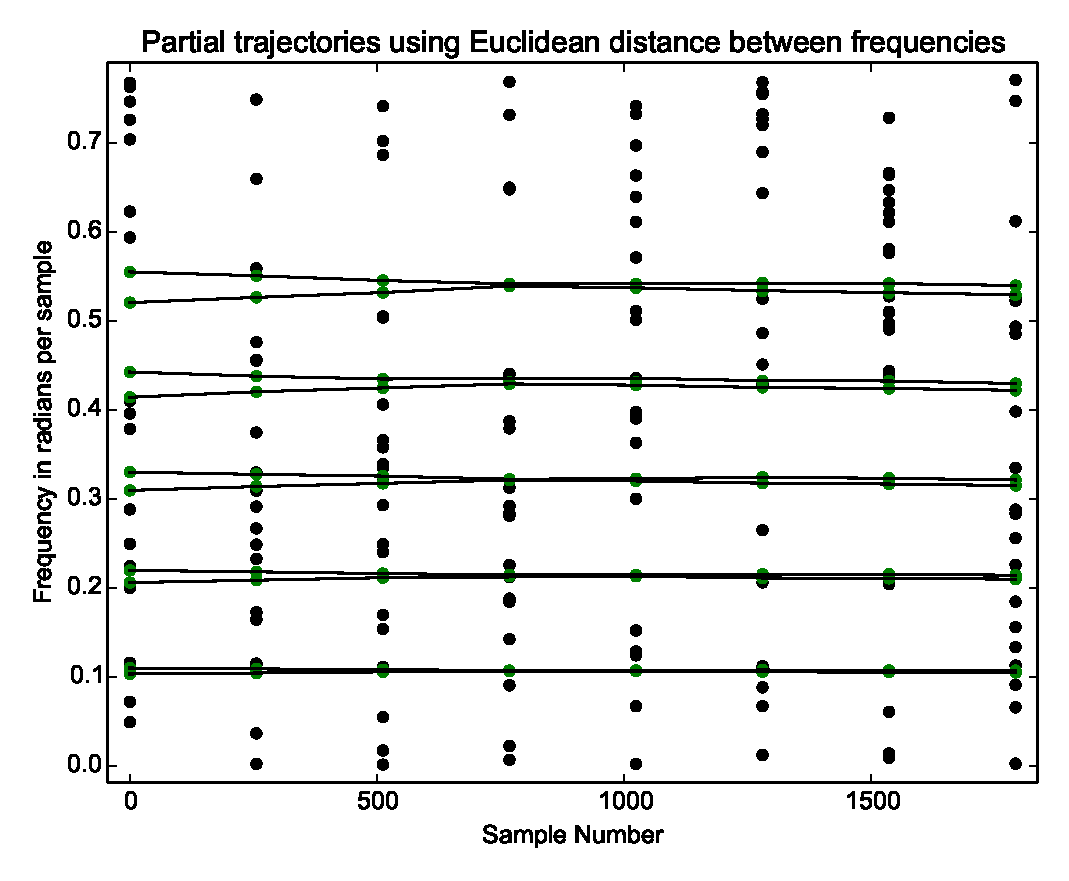
\includegraphics[width=\textwidth]{../experiment_2/plots/lp_ptrack_eudist.eps}
\end{figure}
\begin{figure}
    \centering
    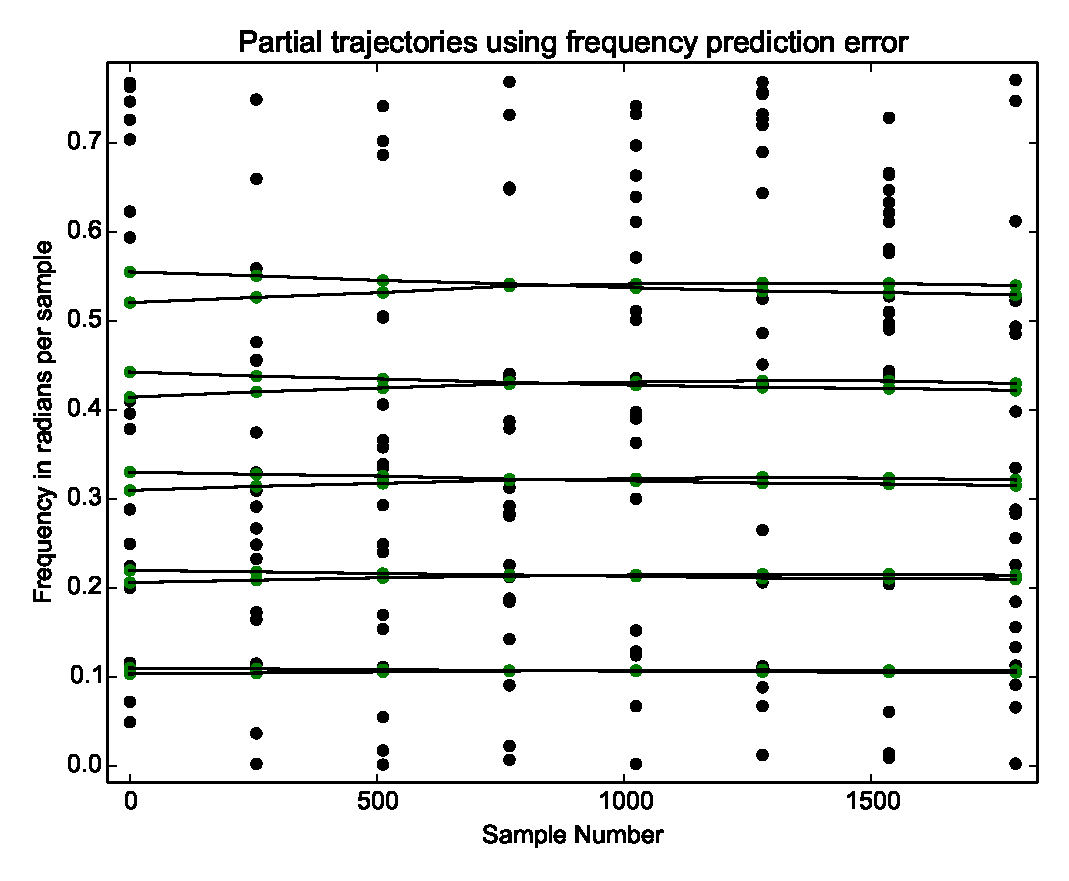
\includegraphics[width=\textwidth]{../experiment_2/plots/lp_ptrack_fpredict.eps}
\end{figure}
%%% Creator: Matplotlib, PGF backend
%%
%% To include the figure in your LaTeX document, write
%%   \input{<filename>.pgf}
%%
%% Make sure the required packages are loaded in your preamble
%%   \usepackage{pgf}
%%
%% Figures using additional raster images can only be included by \input if
%% they are in the same directory as the main LaTeX file. For loading figures
%% from other directories you can use the `import` package
%%   \usepackage{import}
%% and then include the figures with
%%   \import{<path to file>}{<filename>.pgf}
%%
%% Matplotlib used the following preamble
%%   \usepackage{fontspec}
%%   \setmainfont{DejaVu Serif}
%%   \setsansfont{DejaVu Sans}
%%   \setmonofont{DejaVu Sans Mono}
%%
\begingroup%
\makeatletter%
\begin{pgfpicture}%
\pgftransformscale{0.3}
\pgfpathrectangle{\pgfpointorigin}{\pgfqpoint{24.000000in}{14.062500in}}%
\pgfusepath{use as bounding box}%
\begin{pgfscope}%
\pgfsetbuttcap%
\pgfsetroundjoin%
\definecolor{currentfill}{rgb}{1.000000,1.000000,1.000000}%
\pgfsetfillcolor{currentfill}%
\pgfsetlinewidth{0.000000pt}%
\definecolor{currentstroke}{rgb}{1.000000,1.000000,1.000000}%
\pgfsetstrokecolor{currentstroke}%
\pgfsetdash{}{0pt}%
\pgfpathmoveto{\pgfqpoint{0.000000in}{0.000000in}}%
\pgfpathlineto{\pgfqpoint{24.000000in}{0.000000in}}%
\pgfpathlineto{\pgfqpoint{24.000000in}{14.062500in}}%
\pgfpathlineto{\pgfqpoint{0.000000in}{14.062500in}}%
\pgfpathclose%
\pgfusepath{fill}%
\end{pgfscope}%
\begin{pgfscope}%
\pgfsetbuttcap%
\pgfsetroundjoin%
\definecolor{currentfill}{rgb}{1.000000,1.000000,1.000000}%
\pgfsetfillcolor{currentfill}%
\pgfsetlinewidth{0.000000pt}%
\definecolor{currentstroke}{rgb}{0.000000,0.000000,0.000000}%
\pgfsetstrokecolor{currentstroke}%
\pgfsetstrokeopacity{0.000000}%
\pgfsetdash{}{0pt}%
\pgfpathmoveto{\pgfqpoint{3.000000in}{1.406250in}}%
\pgfpathlineto{\pgfqpoint{21.600000in}{1.406250in}}%
\pgfpathlineto{\pgfqpoint{21.600000in}{12.656250in}}%
\pgfpathlineto{\pgfqpoint{3.000000in}{12.656250in}}%
\pgfpathclose%
\pgfusepath{fill}%
\end{pgfscope}%
\begin{pgfscope}%
\pgfpathrectangle{\pgfqpoint{3.000000in}{1.406250in}}{\pgfqpoint{18.600000in}{11.250000in}} %
\pgfusepath{clip}%
\pgfsetbuttcap%
\pgfsetroundjoin%
\definecolor{currentfill}{rgb}{0.000000,0.000000,0.000000}%
\pgfsetfillcolor{currentfill}%
\pgfsetlinewidth{1.003750pt}%
\definecolor{currentstroke}{rgb}{0.000000,0.000000,0.000000}%
\pgfsetstrokecolor{currentstroke}%
\pgfsetdash{}{0pt}%
\pgfpathmoveto{\pgfqpoint{3.181837in}{9.672110in}}%
\pgfpathcurveto{\pgfqpoint{3.190073in}{9.672110in}}{\pgfqpoint{3.197973in}{9.675383in}}{\pgfqpoint{3.203797in}{9.681207in}}%
\pgfpathcurveto{\pgfqpoint{3.209621in}{9.687031in}}{\pgfqpoint{3.212893in}{9.694931in}}{\pgfqpoint{3.212893in}{9.703167in}}%
\pgfpathcurveto{\pgfqpoint{3.212893in}{9.711403in}}{\pgfqpoint{3.209621in}{9.719303in}}{\pgfqpoint{3.203797in}{9.725127in}}%
\pgfpathcurveto{\pgfqpoint{3.197973in}{9.730951in}}{\pgfqpoint{3.190073in}{9.734223in}}{\pgfqpoint{3.181837in}{9.734223in}}%
\pgfpathcurveto{\pgfqpoint{3.173601in}{9.734223in}}{\pgfqpoint{3.165700in}{9.730951in}}{\pgfqpoint{3.159877in}{9.725127in}}%
\pgfpathcurveto{\pgfqpoint{3.154053in}{9.719303in}}{\pgfqpoint{3.150780in}{9.711403in}}{\pgfqpoint{3.150780in}{9.703167in}}%
\pgfpathcurveto{\pgfqpoint{3.150780in}{9.694931in}}{\pgfqpoint{3.154053in}{9.687031in}}{\pgfqpoint{3.159877in}{9.681207in}}%
\pgfpathcurveto{\pgfqpoint{3.165700in}{9.675383in}}{\pgfqpoint{3.173601in}{9.672110in}}{\pgfqpoint{3.181837in}{9.672110in}}%
\pgfpathclose%
\pgfusepath{stroke,fill}%
\end{pgfscope}%
\begin{pgfscope}%
\pgfpathrectangle{\pgfqpoint{3.000000in}{1.406250in}}{\pgfqpoint{18.600000in}{11.250000in}} %
\pgfusepath{clip}%
\pgfsetbuttcap%
\pgfsetroundjoin%
\definecolor{currentfill}{rgb}{0.000000,0.000000,0.000000}%
\pgfsetfillcolor{currentfill}%
\pgfsetlinewidth{1.003750pt}%
\definecolor{currentstroke}{rgb}{0.000000,0.000000,0.000000}%
\pgfsetstrokecolor{currentstroke}%
\pgfsetdash{}{0pt}%
\pgfpathmoveto{\pgfqpoint{3.181837in}{8.555581in}}%
\pgfpathcurveto{\pgfqpoint{3.190073in}{8.555581in}}{\pgfqpoint{3.197973in}{8.558853in}}{\pgfqpoint{3.203797in}{8.564677in}}%
\pgfpathcurveto{\pgfqpoint{3.209621in}{8.570501in}}{\pgfqpoint{3.212893in}{8.578401in}}{\pgfqpoint{3.212893in}{8.586637in}}%
\pgfpathcurveto{\pgfqpoint{3.212893in}{8.594874in}}{\pgfqpoint{3.209621in}{8.602774in}}{\pgfqpoint{3.203797in}{8.608597in}}%
\pgfpathcurveto{\pgfqpoint{3.197973in}{8.614421in}}{\pgfqpoint{3.190073in}{8.617694in}}{\pgfqpoint{3.181837in}{8.617694in}}%
\pgfpathcurveto{\pgfqpoint{3.173601in}{8.617694in}}{\pgfqpoint{3.165700in}{8.614421in}}{\pgfqpoint{3.159877in}{8.608597in}}%
\pgfpathcurveto{\pgfqpoint{3.154053in}{8.602774in}}{\pgfqpoint{3.150780in}{8.594874in}}{\pgfqpoint{3.150780in}{8.586637in}}%
\pgfpathcurveto{\pgfqpoint{3.150780in}{8.578401in}}{\pgfqpoint{3.154053in}{8.570501in}}{\pgfqpoint{3.159877in}{8.564677in}}%
\pgfpathcurveto{\pgfqpoint{3.165700in}{8.558853in}}{\pgfqpoint{3.173601in}{8.555581in}}{\pgfqpoint{3.181837in}{8.555581in}}%
\pgfpathclose%
\pgfusepath{stroke,fill}%
\end{pgfscope}%
\begin{pgfscope}%
\pgfpathrectangle{\pgfqpoint{3.000000in}{1.406250in}}{\pgfqpoint{18.600000in}{11.250000in}} %
\pgfusepath{clip}%
\pgfsetbuttcap%
\pgfsetroundjoin%
\definecolor{currentfill}{rgb}{0.000000,0.000000,0.000000}%
\pgfsetfillcolor{currentfill}%
\pgfsetlinewidth{1.003750pt}%
\definecolor{currentstroke}{rgb}{0.000000,0.000000,0.000000}%
\pgfsetstrokecolor{currentstroke}%
\pgfsetdash{}{0pt}%
\pgfpathmoveto{\pgfqpoint{3.181837in}{17.440805in}}%
\pgfpathcurveto{\pgfqpoint{3.190073in}{17.440805in}}{\pgfqpoint{3.197973in}{17.444077in}}{\pgfqpoint{3.203797in}{17.449901in}}%
\pgfpathcurveto{\pgfqpoint{3.209621in}{17.455725in}}{\pgfqpoint{3.212893in}{17.463625in}}{\pgfqpoint{3.212893in}{17.471861in}}%
\pgfpathcurveto{\pgfqpoint{3.212893in}{17.480097in}}{\pgfqpoint{3.209621in}{17.487997in}}{\pgfqpoint{3.203797in}{17.493821in}}%
\pgfpathcurveto{\pgfqpoint{3.197973in}{17.499645in}}{\pgfqpoint{3.190073in}{17.502918in}}{\pgfqpoint{3.181837in}{17.502918in}}%
\pgfpathcurveto{\pgfqpoint{3.173601in}{17.502918in}}{\pgfqpoint{3.165700in}{17.499645in}}{\pgfqpoint{3.159877in}{17.493821in}}%
\pgfpathcurveto{\pgfqpoint{3.154053in}{17.487997in}}{\pgfqpoint{3.150780in}{17.480097in}}{\pgfqpoint{3.150780in}{17.471861in}}%
\pgfpathcurveto{\pgfqpoint{3.150780in}{17.463625in}}{\pgfqpoint{3.154053in}{17.455725in}}{\pgfqpoint{3.159877in}{17.449901in}}%
\pgfpathcurveto{\pgfqpoint{3.165700in}{17.444077in}}{\pgfqpoint{3.173601in}{17.440805in}}{\pgfqpoint{3.181837in}{17.440805in}}%
\pgfpathclose%
\pgfusepath{stroke,fill}%
\end{pgfscope}%
\begin{pgfscope}%
\pgfpathrectangle{\pgfqpoint{3.000000in}{1.406250in}}{\pgfqpoint{18.600000in}{11.250000in}} %
\pgfusepath{clip}%
\pgfsetbuttcap%
\pgfsetroundjoin%
\definecolor{currentfill}{rgb}{0.000000,0.000000,0.000000}%
\pgfsetfillcolor{currentfill}%
\pgfsetlinewidth{1.003750pt}%
\definecolor{currentstroke}{rgb}{0.000000,0.000000,0.000000}%
\pgfsetstrokecolor{currentstroke}%
\pgfsetdash{}{0pt}%
\pgfpathmoveto{\pgfqpoint{3.181837in}{8.892433in}}%
\pgfpathcurveto{\pgfqpoint{3.190073in}{8.892433in}}{\pgfqpoint{3.197973in}{8.895705in}}{\pgfqpoint{3.203797in}{8.901529in}}%
\pgfpathcurveto{\pgfqpoint{3.209621in}{8.907353in}}{\pgfqpoint{3.212893in}{8.915253in}}{\pgfqpoint{3.212893in}{8.923489in}}%
\pgfpathcurveto{\pgfqpoint{3.212893in}{8.931725in}}{\pgfqpoint{3.209621in}{8.939625in}}{\pgfqpoint{3.203797in}{8.945449in}}%
\pgfpathcurveto{\pgfqpoint{3.197973in}{8.951273in}}{\pgfqpoint{3.190073in}{8.954546in}}{\pgfqpoint{3.181837in}{8.954546in}}%
\pgfpathcurveto{\pgfqpoint{3.173601in}{8.954546in}}{\pgfqpoint{3.165700in}{8.951273in}}{\pgfqpoint{3.159877in}{8.945449in}}%
\pgfpathcurveto{\pgfqpoint{3.154053in}{8.939625in}}{\pgfqpoint{3.150780in}{8.931725in}}{\pgfqpoint{3.150780in}{8.923489in}}%
\pgfpathcurveto{\pgfqpoint{3.150780in}{8.915253in}}{\pgfqpoint{3.154053in}{8.907353in}}{\pgfqpoint{3.159877in}{8.901529in}}%
\pgfpathcurveto{\pgfqpoint{3.165700in}{8.895705in}}{\pgfqpoint{3.173601in}{8.892433in}}{\pgfqpoint{3.181837in}{8.892433in}}%
\pgfpathclose%
\pgfusepath{stroke,fill}%
\end{pgfscope}%
\begin{pgfscope}%
\pgfpathrectangle{\pgfqpoint{3.000000in}{1.406250in}}{\pgfqpoint{18.600000in}{11.250000in}} %
\pgfusepath{clip}%
\pgfsetbuttcap%
\pgfsetroundjoin%
\definecolor{currentfill}{rgb}{0.000000,0.000000,0.000000}%
\pgfsetfillcolor{currentfill}%
\pgfsetlinewidth{1.003750pt}%
\definecolor{currentstroke}{rgb}{0.000000,0.000000,0.000000}%
\pgfsetstrokecolor{currentstroke}%
\pgfsetdash{}{0pt}%
\pgfpathmoveto{\pgfqpoint{3.181837in}{1.722312in}}%
\pgfpathcurveto{\pgfqpoint{3.190073in}{1.722312in}}{\pgfqpoint{3.197973in}{1.725585in}}{\pgfqpoint{3.203797in}{1.731409in}}%
\pgfpathcurveto{\pgfqpoint{3.209621in}{1.737232in}}{\pgfqpoint{3.212893in}{1.745133in}}{\pgfqpoint{3.212893in}{1.753369in}}%
\pgfpathcurveto{\pgfqpoint{3.212893in}{1.761605in}}{\pgfqpoint{3.209621in}{1.769505in}}{\pgfqpoint{3.203797in}{1.775329in}}%
\pgfpathcurveto{\pgfqpoint{3.197973in}{1.781153in}}{\pgfqpoint{3.190073in}{1.784425in}}{\pgfqpoint{3.181837in}{1.784425in}}%
\pgfpathcurveto{\pgfqpoint{3.173601in}{1.784425in}}{\pgfqpoint{3.165700in}{1.781153in}}{\pgfqpoint{3.159877in}{1.775329in}}%
\pgfpathcurveto{\pgfqpoint{3.154053in}{1.769505in}}{\pgfqpoint{3.150780in}{1.761605in}}{\pgfqpoint{3.150780in}{1.753369in}}%
\pgfpathcurveto{\pgfqpoint{3.150780in}{1.745133in}}{\pgfqpoint{3.154053in}{1.737232in}}{\pgfqpoint{3.159877in}{1.731409in}}%
\pgfpathcurveto{\pgfqpoint{3.165700in}{1.725585in}}{\pgfqpoint{3.173601in}{1.722312in}}{\pgfqpoint{3.181837in}{1.722312in}}%
\pgfpathclose%
\pgfusepath{stroke,fill}%
\end{pgfscope}%
\begin{pgfscope}%
\pgfpathrectangle{\pgfqpoint{3.000000in}{1.406250in}}{\pgfqpoint{18.600000in}{11.250000in}} %
\pgfusepath{clip}%
\pgfsetbuttcap%
\pgfsetroundjoin%
\definecolor{currentfill}{rgb}{0.000000,0.000000,0.000000}%
\pgfsetfillcolor{currentfill}%
\pgfsetlinewidth{1.003750pt}%
\definecolor{currentstroke}{rgb}{0.000000,0.000000,0.000000}%
\pgfsetstrokecolor{currentstroke}%
\pgfsetdash{}{0pt}%
\pgfpathmoveto{\pgfqpoint{3.181837in}{4.016151in}}%
\pgfpathcurveto{\pgfqpoint{3.190073in}{4.016151in}}{\pgfqpoint{3.197973in}{4.019423in}}{\pgfqpoint{3.203797in}{4.025247in}}%
\pgfpathcurveto{\pgfqpoint{3.209621in}{4.031071in}}{\pgfqpoint{3.212893in}{4.038971in}}{\pgfqpoint{3.212893in}{4.047207in}}%
\pgfpathcurveto{\pgfqpoint{3.212893in}{4.055444in}}{\pgfqpoint{3.209621in}{4.063344in}}{\pgfqpoint{3.203797in}{4.069168in}}%
\pgfpathcurveto{\pgfqpoint{3.197973in}{4.074991in}}{\pgfqpoint{3.190073in}{4.078264in}}{\pgfqpoint{3.181837in}{4.078264in}}%
\pgfpathcurveto{\pgfqpoint{3.173601in}{4.078264in}}{\pgfqpoint{3.165700in}{4.074991in}}{\pgfqpoint{3.159877in}{4.069168in}}%
\pgfpathcurveto{\pgfqpoint{3.154053in}{4.063344in}}{\pgfqpoint{3.150780in}{4.055444in}}{\pgfqpoint{3.150780in}{4.047207in}}%
\pgfpathcurveto{\pgfqpoint{3.150780in}{4.038971in}}{\pgfqpoint{3.154053in}{4.031071in}}{\pgfqpoint{3.159877in}{4.025247in}}%
\pgfpathcurveto{\pgfqpoint{3.165700in}{4.019423in}}{\pgfqpoint{3.173601in}{4.016151in}}{\pgfqpoint{3.181837in}{4.016151in}}%
\pgfpathclose%
\pgfusepath{stroke,fill}%
\end{pgfscope}%
\begin{pgfscope}%
\pgfpathrectangle{\pgfqpoint{3.000000in}{1.406250in}}{\pgfqpoint{18.600000in}{11.250000in}} %
\pgfusepath{clip}%
\pgfsetbuttcap%
\pgfsetroundjoin%
\definecolor{currentfill}{rgb}{0.000000,0.000000,0.000000}%
\pgfsetfillcolor{currentfill}%
\pgfsetlinewidth{1.003750pt}%
\definecolor{currentstroke}{rgb}{0.000000,0.000000,0.000000}%
\pgfsetstrokecolor{currentstroke}%
\pgfsetdash{}{0pt}%
\pgfpathmoveto{\pgfqpoint{3.181837in}{0.265096in}}%
\pgfpathcurveto{\pgfqpoint{3.190073in}{0.265096in}}{\pgfqpoint{3.197973in}{0.268368in}}{\pgfqpoint{3.203797in}{0.274192in}}%
\pgfpathcurveto{\pgfqpoint{3.209621in}{0.280016in}}{\pgfqpoint{3.212893in}{0.287916in}}{\pgfqpoint{3.212893in}{0.296152in}}%
\pgfpathcurveto{\pgfqpoint{3.212893in}{0.304389in}}{\pgfqpoint{3.209621in}{0.312289in}}{\pgfqpoint{3.203797in}{0.318113in}}%
\pgfpathcurveto{\pgfqpoint{3.197973in}{0.323937in}}{\pgfqpoint{3.190073in}{0.327209in}}{\pgfqpoint{3.181837in}{0.327209in}}%
\pgfpathcurveto{\pgfqpoint{3.173601in}{0.327209in}}{\pgfqpoint{3.165700in}{0.323937in}}{\pgfqpoint{3.159877in}{0.318113in}}%
\pgfpathcurveto{\pgfqpoint{3.154053in}{0.312289in}}{\pgfqpoint{3.150780in}{0.304389in}}{\pgfqpoint{3.150780in}{0.296152in}}%
\pgfpathcurveto{\pgfqpoint{3.150780in}{0.287916in}}{\pgfqpoint{3.154053in}{0.280016in}}{\pgfqpoint{3.159877in}{0.274192in}}%
\pgfpathcurveto{\pgfqpoint{3.165700in}{0.268368in}}{\pgfqpoint{3.173601in}{0.265096in}}{\pgfqpoint{3.181837in}{0.265096in}}%
\pgfpathclose%
\pgfusepath{stroke,fill}%
\end{pgfscope}%
\begin{pgfscope}%
\pgfpathrectangle{\pgfqpoint{3.000000in}{1.406250in}}{\pgfqpoint{18.600000in}{11.250000in}} %
\pgfusepath{clip}%
\pgfsetbuttcap%
\pgfsetroundjoin%
\definecolor{currentfill}{rgb}{0.000000,0.000000,0.000000}%
\pgfsetfillcolor{currentfill}%
\pgfsetlinewidth{1.003750pt}%
\definecolor{currentstroke}{rgb}{0.000000,0.000000,0.000000}%
\pgfsetstrokecolor{currentstroke}%
\pgfsetdash{}{0pt}%
\pgfpathmoveto{\pgfqpoint{3.181837in}{8.144657in}}%
\pgfpathcurveto{\pgfqpoint{3.190073in}{8.144657in}}{\pgfqpoint{3.197973in}{8.147929in}}{\pgfqpoint{3.203797in}{8.153753in}}%
\pgfpathcurveto{\pgfqpoint{3.209621in}{8.159577in}}{\pgfqpoint{3.212893in}{8.167477in}}{\pgfqpoint{3.212893in}{8.175713in}}%
\pgfpathcurveto{\pgfqpoint{3.212893in}{8.183949in}}{\pgfqpoint{3.209621in}{8.191849in}}{\pgfqpoint{3.203797in}{8.197673in}}%
\pgfpathcurveto{\pgfqpoint{3.197973in}{8.203497in}}{\pgfqpoint{3.190073in}{8.206770in}}{\pgfqpoint{3.181837in}{8.206770in}}%
\pgfpathcurveto{\pgfqpoint{3.173601in}{8.206770in}}{\pgfqpoint{3.165700in}{8.203497in}}{\pgfqpoint{3.159877in}{8.197673in}}%
\pgfpathcurveto{\pgfqpoint{3.154053in}{8.191849in}}{\pgfqpoint{3.150780in}{8.183949in}}{\pgfqpoint{3.150780in}{8.175713in}}%
\pgfpathcurveto{\pgfqpoint{3.150780in}{8.167477in}}{\pgfqpoint{3.154053in}{8.159577in}}{\pgfqpoint{3.159877in}{8.153753in}}%
\pgfpathcurveto{\pgfqpoint{3.165700in}{8.147929in}}{\pgfqpoint{3.173601in}{8.144657in}}{\pgfqpoint{3.181837in}{8.144657in}}%
\pgfpathclose%
\pgfusepath{stroke,fill}%
\end{pgfscope}%
\begin{pgfscope}%
\pgfpathrectangle{\pgfqpoint{3.000000in}{1.406250in}}{\pgfqpoint{18.600000in}{11.250000in}} %
\pgfusepath{clip}%
\pgfsetbuttcap%
\pgfsetroundjoin%
\definecolor{currentfill}{rgb}{0.000000,0.000000,0.000000}%
\pgfsetfillcolor{currentfill}%
\pgfsetlinewidth{1.003750pt}%
\definecolor{currentstroke}{rgb}{0.000000,0.000000,0.000000}%
\pgfsetstrokecolor{currentstroke}%
\pgfsetdash{}{0pt}%
\pgfpathmoveto{\pgfqpoint{3.181837in}{16.447853in}}%
\pgfpathcurveto{\pgfqpoint{3.190073in}{16.447853in}}{\pgfqpoint{3.197973in}{16.451125in}}{\pgfqpoint{3.203797in}{16.456949in}}%
\pgfpathcurveto{\pgfqpoint{3.209621in}{16.462773in}}{\pgfqpoint{3.212893in}{16.470673in}}{\pgfqpoint{3.212893in}{16.478909in}}%
\pgfpathcurveto{\pgfqpoint{3.212893in}{16.487145in}}{\pgfqpoint{3.209621in}{16.495045in}}{\pgfqpoint{3.203797in}{16.500869in}}%
\pgfpathcurveto{\pgfqpoint{3.197973in}{16.506693in}}{\pgfqpoint{3.190073in}{16.509966in}}{\pgfqpoint{3.181837in}{16.509966in}}%
\pgfpathcurveto{\pgfqpoint{3.173601in}{16.509966in}}{\pgfqpoint{3.165700in}{16.506693in}}{\pgfqpoint{3.159877in}{16.500869in}}%
\pgfpathcurveto{\pgfqpoint{3.154053in}{16.495045in}}{\pgfqpoint{3.150780in}{16.487145in}}{\pgfqpoint{3.150780in}{16.478909in}}%
\pgfpathcurveto{\pgfqpoint{3.150780in}{16.470673in}}{\pgfqpoint{3.154053in}{16.462773in}}{\pgfqpoint{3.159877in}{16.456949in}}%
\pgfpathcurveto{\pgfqpoint{3.165700in}{16.451125in}}{\pgfqpoint{3.173601in}{16.447853in}}{\pgfqpoint{3.181837in}{16.447853in}}%
\pgfpathclose%
\pgfusepath{stroke,fill}%
\end{pgfscope}%
\begin{pgfscope}%
\pgfpathrectangle{\pgfqpoint{3.000000in}{1.406250in}}{\pgfqpoint{18.600000in}{11.250000in}} %
\pgfusepath{clip}%
\pgfsetbuttcap%
\pgfsetroundjoin%
\definecolor{currentfill}{rgb}{0.000000,0.000000,0.000000}%
\pgfsetfillcolor{currentfill}%
\pgfsetlinewidth{1.003750pt}%
\definecolor{currentstroke}{rgb}{0.000000,0.000000,0.000000}%
\pgfsetstrokecolor{currentstroke}%
\pgfsetdash{}{0pt}%
\pgfpathmoveto{\pgfqpoint{3.181837in}{11.535123in}}%
\pgfpathcurveto{\pgfqpoint{3.190073in}{11.535123in}}{\pgfqpoint{3.197973in}{11.538395in}}{\pgfqpoint{3.203797in}{11.544219in}}%
\pgfpathcurveto{\pgfqpoint{3.209621in}{11.550043in}}{\pgfqpoint{3.212893in}{11.557943in}}{\pgfqpoint{3.212893in}{11.566180in}}%
\pgfpathcurveto{\pgfqpoint{3.212893in}{11.574416in}}{\pgfqpoint{3.209621in}{11.582316in}}{\pgfqpoint{3.203797in}{11.588140in}}%
\pgfpathcurveto{\pgfqpoint{3.197973in}{11.593964in}}{\pgfqpoint{3.190073in}{11.597236in}}{\pgfqpoint{3.181837in}{11.597236in}}%
\pgfpathcurveto{\pgfqpoint{3.173601in}{11.597236in}}{\pgfqpoint{3.165700in}{11.593964in}}{\pgfqpoint{3.159877in}{11.588140in}}%
\pgfpathcurveto{\pgfqpoint{3.154053in}{11.582316in}}{\pgfqpoint{3.150780in}{11.574416in}}{\pgfqpoint{3.150780in}{11.566180in}}%
\pgfpathcurveto{\pgfqpoint{3.150780in}{11.557943in}}{\pgfqpoint{3.154053in}{11.550043in}}{\pgfqpoint{3.159877in}{11.544219in}}%
\pgfpathcurveto{\pgfqpoint{3.165700in}{11.538395in}}{\pgfqpoint{3.173601in}{11.535123in}}{\pgfqpoint{3.181837in}{11.535123in}}%
\pgfpathclose%
\pgfusepath{stroke,fill}%
\end{pgfscope}%
\begin{pgfscope}%
\pgfpathrectangle{\pgfqpoint{3.000000in}{1.406250in}}{\pgfqpoint{18.600000in}{11.250000in}} %
\pgfusepath{clip}%
\pgfsetbuttcap%
\pgfsetroundjoin%
\definecolor{currentfill}{rgb}{0.000000,0.000000,0.000000}%
\pgfsetfillcolor{currentfill}%
\pgfsetlinewidth{1.003750pt}%
\definecolor{currentstroke}{rgb}{0.000000,0.000000,0.000000}%
\pgfsetstrokecolor{currentstroke}%
\pgfsetdash{}{0pt}%
\pgfpathmoveto{\pgfqpoint{3.181837in}{0.814871in}}%
\pgfpathcurveto{\pgfqpoint{3.190073in}{0.814871in}}{\pgfqpoint{3.197973in}{0.818143in}}{\pgfqpoint{3.203797in}{0.823967in}}%
\pgfpathcurveto{\pgfqpoint{3.209621in}{0.829791in}}{\pgfqpoint{3.212893in}{0.837691in}}{\pgfqpoint{3.212893in}{0.845927in}}%
\pgfpathcurveto{\pgfqpoint{3.212893in}{0.854164in}}{\pgfqpoint{3.209621in}{0.862064in}}{\pgfqpoint{3.203797in}{0.867887in}}%
\pgfpathcurveto{\pgfqpoint{3.197973in}{0.873711in}}{\pgfqpoint{3.190073in}{0.876984in}}{\pgfqpoint{3.181837in}{0.876984in}}%
\pgfpathcurveto{\pgfqpoint{3.173601in}{0.876984in}}{\pgfqpoint{3.165700in}{0.873711in}}{\pgfqpoint{3.159877in}{0.867887in}}%
\pgfpathcurveto{\pgfqpoint{3.154053in}{0.862064in}}{\pgfqpoint{3.150780in}{0.854164in}}{\pgfqpoint{3.150780in}{0.845927in}}%
\pgfpathcurveto{\pgfqpoint{3.150780in}{0.837691in}}{\pgfqpoint{3.154053in}{0.829791in}}{\pgfqpoint{3.159877in}{0.823967in}}%
\pgfpathcurveto{\pgfqpoint{3.165700in}{0.818143in}}{\pgfqpoint{3.173601in}{0.814871in}}{\pgfqpoint{3.181837in}{0.814871in}}%
\pgfpathclose%
\pgfusepath{stroke,fill}%
\end{pgfscope}%
\begin{pgfscope}%
\pgfpathrectangle{\pgfqpoint{3.000000in}{1.406250in}}{\pgfqpoint{18.600000in}{11.250000in}} %
\pgfusepath{clip}%
\pgfsetbuttcap%
\pgfsetroundjoin%
\definecolor{currentfill}{rgb}{0.000000,0.000000,0.000000}%
\pgfsetfillcolor{currentfill}%
\pgfsetlinewidth{1.003750pt}%
\definecolor{currentstroke}{rgb}{0.000000,0.000000,0.000000}%
\pgfsetstrokecolor{currentstroke}%
\pgfsetdash{}{0pt}%
\pgfpathmoveto{\pgfqpoint{3.181837in}{12.359729in}}%
\pgfpathcurveto{\pgfqpoint{3.190073in}{12.359729in}}{\pgfqpoint{3.197973in}{12.363001in}}{\pgfqpoint{3.203797in}{12.368825in}}%
\pgfpathcurveto{\pgfqpoint{3.209621in}{12.374649in}}{\pgfqpoint{3.212893in}{12.382549in}}{\pgfqpoint{3.212893in}{12.390785in}}%
\pgfpathcurveto{\pgfqpoint{3.212893in}{12.399022in}}{\pgfqpoint{3.209621in}{12.406922in}}{\pgfqpoint{3.203797in}{12.412746in}}%
\pgfpathcurveto{\pgfqpoint{3.197973in}{12.418570in}}{\pgfqpoint{3.190073in}{12.421842in}}{\pgfqpoint{3.181837in}{12.421842in}}%
\pgfpathcurveto{\pgfqpoint{3.173601in}{12.421842in}}{\pgfqpoint{3.165700in}{12.418570in}}{\pgfqpoint{3.159877in}{12.412746in}}%
\pgfpathcurveto{\pgfqpoint{3.154053in}{12.406922in}}{\pgfqpoint{3.150780in}{12.399022in}}{\pgfqpoint{3.150780in}{12.390785in}}%
\pgfpathcurveto{\pgfqpoint{3.150780in}{12.382549in}}{\pgfqpoint{3.154053in}{12.374649in}}{\pgfqpoint{3.159877in}{12.368825in}}%
\pgfpathcurveto{\pgfqpoint{3.165700in}{12.363001in}}{\pgfqpoint{3.173601in}{12.359729in}}{\pgfqpoint{3.181837in}{12.359729in}}%
\pgfpathclose%
\pgfusepath{stroke,fill}%
\end{pgfscope}%
\begin{pgfscope}%
\pgfpathrectangle{\pgfqpoint{3.000000in}{1.406250in}}{\pgfqpoint{18.600000in}{11.250000in}} %
\pgfusepath{clip}%
\pgfsetbuttcap%
\pgfsetroundjoin%
\definecolor{currentfill}{rgb}{0.000000,0.000000,0.000000}%
\pgfsetfillcolor{currentfill}%
\pgfsetlinewidth{1.003750pt}%
\definecolor{currentstroke}{rgb}{0.000000,0.000000,0.000000}%
\pgfsetstrokecolor{currentstroke}%
\pgfsetdash{}{0pt}%
\pgfpathmoveto{\pgfqpoint{3.181837in}{6.983986in}}%
\pgfpathcurveto{\pgfqpoint{3.190073in}{6.983986in}}{\pgfqpoint{3.197973in}{6.987259in}}{\pgfqpoint{3.203797in}{6.993083in}}%
\pgfpathcurveto{\pgfqpoint{3.209621in}{6.998907in}}{\pgfqpoint{3.212893in}{7.006807in}}{\pgfqpoint{3.212893in}{7.015043in}}%
\pgfpathcurveto{\pgfqpoint{3.212893in}{7.023279in}}{\pgfqpoint{3.209621in}{7.031179in}}{\pgfqpoint{3.203797in}{7.037003in}}%
\pgfpathcurveto{\pgfqpoint{3.197973in}{7.042827in}}{\pgfqpoint{3.190073in}{7.046099in}}{\pgfqpoint{3.181837in}{7.046099in}}%
\pgfpathcurveto{\pgfqpoint{3.173601in}{7.046099in}}{\pgfqpoint{3.165700in}{7.042827in}}{\pgfqpoint{3.159877in}{7.037003in}}%
\pgfpathcurveto{\pgfqpoint{3.154053in}{7.031179in}}{\pgfqpoint{3.150780in}{7.023279in}}{\pgfqpoint{3.150780in}{7.015043in}}%
\pgfpathcurveto{\pgfqpoint{3.150780in}{7.006807in}}{\pgfqpoint{3.154053in}{6.998907in}}{\pgfqpoint{3.159877in}{6.993083in}}%
\pgfpathcurveto{\pgfqpoint{3.165700in}{6.987259in}}{\pgfqpoint{3.173601in}{6.983986in}}{\pgfqpoint{3.181837in}{6.983986in}}%
\pgfpathclose%
\pgfusepath{stroke,fill}%
\end{pgfscope}%
\begin{pgfscope}%
\pgfpathrectangle{\pgfqpoint{3.000000in}{1.406250in}}{\pgfqpoint{18.600000in}{11.250000in}} %
\pgfusepath{clip}%
\pgfsetbuttcap%
\pgfsetroundjoin%
\definecolor{currentfill}{rgb}{0.000000,0.000000,0.000000}%
\pgfsetfillcolor{currentfill}%
\pgfsetlinewidth{1.003750pt}%
\definecolor{currentstroke}{rgb}{0.000000,0.000000,0.000000}%
\pgfsetstrokecolor{currentstroke}%
\pgfsetdash{}{0pt}%
\pgfpathmoveto{\pgfqpoint{3.181837in}{1.618001in}}%
\pgfpathcurveto{\pgfqpoint{3.190073in}{1.618001in}}{\pgfqpoint{3.197973in}{1.621273in}}{\pgfqpoint{3.203797in}{1.627097in}}%
\pgfpathcurveto{\pgfqpoint{3.209621in}{1.632921in}}{\pgfqpoint{3.212893in}{1.640821in}}{\pgfqpoint{3.212893in}{1.649057in}}%
\pgfpathcurveto{\pgfqpoint{3.212893in}{1.657294in}}{\pgfqpoint{3.209621in}{1.665194in}}{\pgfqpoint{3.203797in}{1.671018in}}%
\pgfpathcurveto{\pgfqpoint{3.197973in}{1.676842in}}{\pgfqpoint{3.190073in}{1.680114in}}{\pgfqpoint{3.181837in}{1.680114in}}%
\pgfpathcurveto{\pgfqpoint{3.173601in}{1.680114in}}{\pgfqpoint{3.165700in}{1.676842in}}{\pgfqpoint{3.159877in}{1.671018in}}%
\pgfpathcurveto{\pgfqpoint{3.154053in}{1.665194in}}{\pgfqpoint{3.150780in}{1.657294in}}{\pgfqpoint{3.150780in}{1.649057in}}%
\pgfpathcurveto{\pgfqpoint{3.150780in}{1.640821in}}{\pgfqpoint{3.154053in}{1.632921in}}{\pgfqpoint{3.159877in}{1.627097in}}%
\pgfpathcurveto{\pgfqpoint{3.165700in}{1.621273in}}{\pgfqpoint{3.173601in}{1.618001in}}{\pgfqpoint{3.181837in}{1.618001in}}%
\pgfpathclose%
\pgfusepath{stroke,fill}%
\end{pgfscope}%
\begin{pgfscope}%
\pgfpathrectangle{\pgfqpoint{3.000000in}{1.406250in}}{\pgfqpoint{18.600000in}{11.250000in}} %
\pgfusepath{clip}%
\pgfsetbuttcap%
\pgfsetroundjoin%
\definecolor{currentfill}{rgb}{0.000000,0.000000,0.000000}%
\pgfsetfillcolor{currentfill}%
\pgfsetlinewidth{1.003750pt}%
\definecolor{currentstroke}{rgb}{0.000000,0.000000,0.000000}%
\pgfsetstrokecolor{currentstroke}%
\pgfsetdash{}{0pt}%
\pgfpathmoveto{\pgfqpoint{3.181837in}{4.343959in}}%
\pgfpathcurveto{\pgfqpoint{3.190073in}{4.343959in}}{\pgfqpoint{3.197973in}{4.347231in}}{\pgfqpoint{3.203797in}{4.353055in}}%
\pgfpathcurveto{\pgfqpoint{3.209621in}{4.358879in}}{\pgfqpoint{3.212893in}{4.366779in}}{\pgfqpoint{3.212893in}{4.375016in}}%
\pgfpathcurveto{\pgfqpoint{3.212893in}{4.383252in}}{\pgfqpoint{3.209621in}{4.391152in}}{\pgfqpoint{3.203797in}{4.396976in}}%
\pgfpathcurveto{\pgfqpoint{3.197973in}{4.402800in}}{\pgfqpoint{3.190073in}{4.406072in}}{\pgfqpoint{3.181837in}{4.406072in}}%
\pgfpathcurveto{\pgfqpoint{3.173601in}{4.406072in}}{\pgfqpoint{3.165700in}{4.402800in}}{\pgfqpoint{3.159877in}{4.396976in}}%
\pgfpathcurveto{\pgfqpoint{3.154053in}{4.391152in}}{\pgfqpoint{3.150780in}{4.383252in}}{\pgfqpoint{3.150780in}{4.375016in}}%
\pgfpathcurveto{\pgfqpoint{3.150780in}{4.366779in}}{\pgfqpoint{3.154053in}{4.358879in}}{\pgfqpoint{3.159877in}{4.353055in}}%
\pgfpathcurveto{\pgfqpoint{3.165700in}{4.347231in}}{\pgfqpoint{3.173601in}{4.343959in}}{\pgfqpoint{3.181837in}{4.343959in}}%
\pgfpathclose%
\pgfusepath{stroke,fill}%
\end{pgfscope}%
\begin{pgfscope}%
\pgfpathrectangle{\pgfqpoint{3.000000in}{1.406250in}}{\pgfqpoint{18.600000in}{11.250000in}} %
\pgfusepath{clip}%
\pgfsetbuttcap%
\pgfsetroundjoin%
\definecolor{currentfill}{rgb}{0.000000,0.000000,0.000000}%
\pgfsetfillcolor{currentfill}%
\pgfsetlinewidth{1.003750pt}%
\definecolor{currentstroke}{rgb}{0.000000,0.000000,0.000000}%
\pgfsetstrokecolor{currentstroke}%
\pgfsetdash{}{0pt}%
\pgfpathmoveto{\pgfqpoint{3.181837in}{6.492435in}}%
\pgfpathcurveto{\pgfqpoint{3.190073in}{6.492435in}}{\pgfqpoint{3.197973in}{6.495707in}}{\pgfqpoint{3.203797in}{6.501531in}}%
\pgfpathcurveto{\pgfqpoint{3.209621in}{6.507355in}}{\pgfqpoint{3.212893in}{6.515255in}}{\pgfqpoint{3.212893in}{6.523492in}}%
\pgfpathcurveto{\pgfqpoint{3.212893in}{6.531728in}}{\pgfqpoint{3.209621in}{6.539628in}}{\pgfqpoint{3.203797in}{6.545452in}}%
\pgfpathcurveto{\pgfqpoint{3.197973in}{6.551276in}}{\pgfqpoint{3.190073in}{6.554548in}}{\pgfqpoint{3.181837in}{6.554548in}}%
\pgfpathcurveto{\pgfqpoint{3.173601in}{6.554548in}}{\pgfqpoint{3.165700in}{6.551276in}}{\pgfqpoint{3.159877in}{6.545452in}}%
\pgfpathcurveto{\pgfqpoint{3.154053in}{6.539628in}}{\pgfqpoint{3.150780in}{6.531728in}}{\pgfqpoint{3.150780in}{6.523492in}}%
\pgfpathcurveto{\pgfqpoint{3.150780in}{6.515255in}}{\pgfqpoint{3.154053in}{6.507355in}}{\pgfqpoint{3.159877in}{6.501531in}}%
\pgfpathcurveto{\pgfqpoint{3.165700in}{6.495707in}}{\pgfqpoint{3.173601in}{6.492435in}}{\pgfqpoint{3.181837in}{6.492435in}}%
\pgfpathclose%
\pgfusepath{stroke,fill}%
\end{pgfscope}%
\begin{pgfscope}%
\pgfpathrectangle{\pgfqpoint{3.000000in}{1.406250in}}{\pgfqpoint{18.600000in}{11.250000in}} %
\pgfusepath{clip}%
\pgfsetbuttcap%
\pgfsetroundjoin%
\definecolor{currentfill}{rgb}{0.000000,0.000000,0.000000}%
\pgfsetfillcolor{currentfill}%
\pgfsetlinewidth{1.003750pt}%
\definecolor{currentstroke}{rgb}{0.000000,0.000000,0.000000}%
\pgfsetstrokecolor{currentstroke}%
\pgfsetdash{}{0pt}%
\pgfpathmoveto{\pgfqpoint{3.181837in}{5.981283in}}%
\pgfpathcurveto{\pgfqpoint{3.190073in}{5.981283in}}{\pgfqpoint{3.197973in}{5.984556in}}{\pgfqpoint{3.203797in}{5.990379in}}%
\pgfpathcurveto{\pgfqpoint{3.209621in}{5.996203in}}{\pgfqpoint{3.212893in}{6.004103in}}{\pgfqpoint{3.212893in}{6.012340in}}%
\pgfpathcurveto{\pgfqpoint{3.212893in}{6.020576in}}{\pgfqpoint{3.209621in}{6.028476in}}{\pgfqpoint{3.203797in}{6.034300in}}%
\pgfpathcurveto{\pgfqpoint{3.197973in}{6.040124in}}{\pgfqpoint{3.190073in}{6.043396in}}{\pgfqpoint{3.181837in}{6.043396in}}%
\pgfpathcurveto{\pgfqpoint{3.173601in}{6.043396in}}{\pgfqpoint{3.165700in}{6.040124in}}{\pgfqpoint{3.159877in}{6.034300in}}%
\pgfpathcurveto{\pgfqpoint{3.154053in}{6.028476in}}{\pgfqpoint{3.150780in}{6.020576in}}{\pgfqpoint{3.150780in}{6.012340in}}%
\pgfpathcurveto{\pgfqpoint{3.150780in}{6.004103in}}{\pgfqpoint{3.154053in}{5.996203in}}{\pgfqpoint{3.159877in}{5.990379in}}%
\pgfpathcurveto{\pgfqpoint{3.165700in}{5.984556in}}{\pgfqpoint{3.173601in}{5.981283in}}{\pgfqpoint{3.181837in}{5.981283in}}%
\pgfpathclose%
\pgfusepath{stroke,fill}%
\end{pgfscope}%
\begin{pgfscope}%
\pgfpathrectangle{\pgfqpoint{3.000000in}{1.406250in}}{\pgfqpoint{18.600000in}{11.250000in}} %
\pgfusepath{clip}%
\pgfsetbuttcap%
\pgfsetroundjoin%
\definecolor{currentfill}{rgb}{0.000000,0.000000,0.000000}%
\pgfsetfillcolor{currentfill}%
\pgfsetlinewidth{1.003750pt}%
\definecolor{currentstroke}{rgb}{0.000000,0.000000,0.000000}%
\pgfsetstrokecolor{currentstroke}%
\pgfsetdash{}{0pt}%
\pgfpathmoveto{\pgfqpoint{3.181837in}{17.330040in}}%
\pgfpathcurveto{\pgfqpoint{3.190073in}{17.330040in}}{\pgfqpoint{3.197973in}{17.333312in}}{\pgfqpoint{3.203797in}{17.339136in}}%
\pgfpathcurveto{\pgfqpoint{3.209621in}{17.344960in}}{\pgfqpoint{3.212893in}{17.352860in}}{\pgfqpoint{3.212893in}{17.361096in}}%
\pgfpathcurveto{\pgfqpoint{3.212893in}{17.369333in}}{\pgfqpoint{3.209621in}{17.377233in}}{\pgfqpoint{3.203797in}{17.383057in}}%
\pgfpathcurveto{\pgfqpoint{3.197973in}{17.388881in}}{\pgfqpoint{3.190073in}{17.392153in}}{\pgfqpoint{3.181837in}{17.392153in}}%
\pgfpathcurveto{\pgfqpoint{3.173601in}{17.392153in}}{\pgfqpoint{3.165700in}{17.388881in}}{\pgfqpoint{3.159877in}{17.383057in}}%
\pgfpathcurveto{\pgfqpoint{3.154053in}{17.377233in}}{\pgfqpoint{3.150780in}{17.369333in}}{\pgfqpoint{3.150780in}{17.361096in}}%
\pgfpathcurveto{\pgfqpoint{3.150780in}{17.352860in}}{\pgfqpoint{3.154053in}{17.344960in}}{\pgfqpoint{3.159877in}{17.339136in}}%
\pgfpathcurveto{\pgfqpoint{3.165700in}{17.333312in}}{\pgfqpoint{3.173601in}{17.330040in}}{\pgfqpoint{3.181837in}{17.330040in}}%
\pgfpathclose%
\pgfusepath{stroke,fill}%
\end{pgfscope}%
\begin{pgfscope}%
\pgfpathrectangle{\pgfqpoint{3.000000in}{1.406250in}}{\pgfqpoint{18.600000in}{11.250000in}} %
\pgfusepath{clip}%
\pgfsetbuttcap%
\pgfsetroundjoin%
\definecolor{currentfill}{rgb}{0.000000,0.000000,0.000000}%
\pgfsetfillcolor{currentfill}%
\pgfsetlinewidth{1.003750pt}%
\definecolor{currentstroke}{rgb}{0.000000,0.000000,0.000000}%
\pgfsetstrokecolor{currentstroke}%
\pgfsetdash{}{0pt}%
\pgfpathmoveto{\pgfqpoint{3.181837in}{1.864388in}}%
\pgfpathcurveto{\pgfqpoint{3.190073in}{1.864388in}}{\pgfqpoint{3.197973in}{1.867660in}}{\pgfqpoint{3.203797in}{1.873484in}}%
\pgfpathcurveto{\pgfqpoint{3.209621in}{1.879308in}}{\pgfqpoint{3.212893in}{1.887208in}}{\pgfqpoint{3.212893in}{1.895444in}}%
\pgfpathcurveto{\pgfqpoint{3.212893in}{1.903681in}}{\pgfqpoint{3.209621in}{1.911581in}}{\pgfqpoint{3.203797in}{1.917405in}}%
\pgfpathcurveto{\pgfqpoint{3.197973in}{1.923229in}}{\pgfqpoint{3.190073in}{1.926501in}}{\pgfqpoint{3.181837in}{1.926501in}}%
\pgfpathcurveto{\pgfqpoint{3.173601in}{1.926501in}}{\pgfqpoint{3.165700in}{1.923229in}}{\pgfqpoint{3.159877in}{1.917405in}}%
\pgfpathcurveto{\pgfqpoint{3.154053in}{1.911581in}}{\pgfqpoint{3.150780in}{1.903681in}}{\pgfqpoint{3.150780in}{1.895444in}}%
\pgfpathcurveto{\pgfqpoint{3.150780in}{1.887208in}}{\pgfqpoint{3.154053in}{1.879308in}}{\pgfqpoint{3.159877in}{1.873484in}}%
\pgfpathcurveto{\pgfqpoint{3.165700in}{1.867660in}}{\pgfqpoint{3.173601in}{1.864388in}}{\pgfqpoint{3.181837in}{1.864388in}}%
\pgfpathclose%
\pgfusepath{stroke,fill}%
\end{pgfscope}%
\begin{pgfscope}%
\pgfpathrectangle{\pgfqpoint{3.000000in}{1.406250in}}{\pgfqpoint{18.600000in}{11.250000in}} %
\pgfusepath{clip}%
\pgfsetbuttcap%
\pgfsetroundjoin%
\definecolor{currentfill}{rgb}{0.000000,0.000000,0.000000}%
\pgfsetfillcolor{currentfill}%
\pgfsetlinewidth{1.003750pt}%
\definecolor{currentstroke}{rgb}{0.000000,0.000000,0.000000}%
\pgfsetstrokecolor{currentstroke}%
\pgfsetdash{}{0pt}%
\pgfpathmoveto{\pgfqpoint{3.181837in}{1.561616in}}%
\pgfpathcurveto{\pgfqpoint{3.190073in}{1.561616in}}{\pgfqpoint{3.197973in}{1.564888in}}{\pgfqpoint{3.203797in}{1.570712in}}%
\pgfpathcurveto{\pgfqpoint{3.209621in}{1.576536in}}{\pgfqpoint{3.212893in}{1.584436in}}{\pgfqpoint{3.212893in}{1.592673in}}%
\pgfpathcurveto{\pgfqpoint{3.212893in}{1.600909in}}{\pgfqpoint{3.209621in}{1.608809in}}{\pgfqpoint{3.203797in}{1.614633in}}%
\pgfpathcurveto{\pgfqpoint{3.197973in}{1.620457in}}{\pgfqpoint{3.190073in}{1.623729in}}{\pgfqpoint{3.181837in}{1.623729in}}%
\pgfpathcurveto{\pgfqpoint{3.173601in}{1.623729in}}{\pgfqpoint{3.165700in}{1.620457in}}{\pgfqpoint{3.159877in}{1.614633in}}%
\pgfpathcurveto{\pgfqpoint{3.154053in}{1.608809in}}{\pgfqpoint{3.150780in}{1.600909in}}{\pgfqpoint{3.150780in}{1.592673in}}%
\pgfpathcurveto{\pgfqpoint{3.150780in}{1.584436in}}{\pgfqpoint{3.154053in}{1.576536in}}{\pgfqpoint{3.159877in}{1.570712in}}%
\pgfpathcurveto{\pgfqpoint{3.165700in}{1.564888in}}{\pgfqpoint{3.173601in}{1.561616in}}{\pgfqpoint{3.181837in}{1.561616in}}%
\pgfpathclose%
\pgfusepath{stroke,fill}%
\end{pgfscope}%
\begin{pgfscope}%
\pgfpathrectangle{\pgfqpoint{3.000000in}{1.406250in}}{\pgfqpoint{18.600000in}{11.250000in}} %
\pgfusepath{clip}%
\pgfsetbuttcap%
\pgfsetroundjoin%
\definecolor{currentfill}{rgb}{0.000000,0.000000,0.000000}%
\pgfsetfillcolor{currentfill}%
\pgfsetlinewidth{1.003750pt}%
\definecolor{currentstroke}{rgb}{0.000000,0.000000,0.000000}%
\pgfsetstrokecolor{currentstroke}%
\pgfsetdash{}{0pt}%
\pgfpathmoveto{\pgfqpoint{3.181837in}{4.456394in}}%
\pgfpathcurveto{\pgfqpoint{3.190073in}{4.456394in}}{\pgfqpoint{3.197973in}{4.459666in}}{\pgfqpoint{3.203797in}{4.465490in}}%
\pgfpathcurveto{\pgfqpoint{3.209621in}{4.471314in}}{\pgfqpoint{3.212893in}{4.479214in}}{\pgfqpoint{3.212893in}{4.487451in}}%
\pgfpathcurveto{\pgfqpoint{3.212893in}{4.495687in}}{\pgfqpoint{3.209621in}{4.503587in}}{\pgfqpoint{3.203797in}{4.509411in}}%
\pgfpathcurveto{\pgfqpoint{3.197973in}{4.515235in}}{\pgfqpoint{3.190073in}{4.518507in}}{\pgfqpoint{3.181837in}{4.518507in}}%
\pgfpathcurveto{\pgfqpoint{3.173601in}{4.518507in}}{\pgfqpoint{3.165700in}{4.515235in}}{\pgfqpoint{3.159877in}{4.509411in}}%
\pgfpathcurveto{\pgfqpoint{3.154053in}{4.503587in}}{\pgfqpoint{3.150780in}{4.495687in}}{\pgfqpoint{3.150780in}{4.487451in}}%
\pgfpathcurveto{\pgfqpoint{3.150780in}{4.479214in}}{\pgfqpoint{3.154053in}{4.471314in}}{\pgfqpoint{3.159877in}{4.465490in}}%
\pgfpathcurveto{\pgfqpoint{3.165700in}{4.459666in}}{\pgfqpoint{3.173601in}{4.456394in}}{\pgfqpoint{3.181837in}{4.456394in}}%
\pgfpathclose%
\pgfusepath{stroke,fill}%
\end{pgfscope}%
\begin{pgfscope}%
\pgfpathrectangle{\pgfqpoint{3.000000in}{1.406250in}}{\pgfqpoint{18.600000in}{11.250000in}} %
\pgfusepath{clip}%
\pgfsetbuttcap%
\pgfsetroundjoin%
\definecolor{currentfill}{rgb}{0.000000,0.000000,0.000000}%
\pgfsetfillcolor{currentfill}%
\pgfsetlinewidth{1.003750pt}%
\definecolor{currentstroke}{rgb}{0.000000,0.000000,0.000000}%
\pgfsetstrokecolor{currentstroke}%
\pgfsetdash{}{0pt}%
\pgfpathmoveto{\pgfqpoint{3.181837in}{3.874887in}}%
\pgfpathcurveto{\pgfqpoint{3.190073in}{3.874887in}}{\pgfqpoint{3.197973in}{3.878160in}}{\pgfqpoint{3.203797in}{3.883984in}}%
\pgfpathcurveto{\pgfqpoint{3.209621in}{3.889808in}}{\pgfqpoint{3.212893in}{3.897708in}}{\pgfqpoint{3.212893in}{3.905944in}}%
\pgfpathcurveto{\pgfqpoint{3.212893in}{3.914180in}}{\pgfqpoint{3.209621in}{3.922080in}}{\pgfqpoint{3.203797in}{3.927904in}}%
\pgfpathcurveto{\pgfqpoint{3.197973in}{3.933728in}}{\pgfqpoint{3.190073in}{3.937000in}}{\pgfqpoint{3.181837in}{3.937000in}}%
\pgfpathcurveto{\pgfqpoint{3.173601in}{3.937000in}}{\pgfqpoint{3.165700in}{3.933728in}}{\pgfqpoint{3.159877in}{3.927904in}}%
\pgfpathcurveto{\pgfqpoint{3.154053in}{3.922080in}}{\pgfqpoint{3.150780in}{3.914180in}}{\pgfqpoint{3.150780in}{3.905944in}}%
\pgfpathcurveto{\pgfqpoint{3.150780in}{3.897708in}}{\pgfqpoint{3.154053in}{3.889808in}}{\pgfqpoint{3.159877in}{3.883984in}}%
\pgfpathcurveto{\pgfqpoint{3.165700in}{3.878160in}}{\pgfqpoint{3.173601in}{3.874887in}}{\pgfqpoint{3.181837in}{3.874887in}}%
\pgfpathclose%
\pgfusepath{stroke,fill}%
\end{pgfscope}%
\begin{pgfscope}%
\pgfpathrectangle{\pgfqpoint{3.000000in}{1.406250in}}{\pgfqpoint{18.600000in}{11.250000in}} %
\pgfusepath{clip}%
\pgfsetbuttcap%
\pgfsetroundjoin%
\definecolor{currentfill}{rgb}{0.000000,0.000000,0.000000}%
\pgfsetfillcolor{currentfill}%
\pgfsetlinewidth{1.003750pt}%
\definecolor{currentstroke}{rgb}{0.000000,0.000000,0.000000}%
\pgfsetstrokecolor{currentstroke}%
\pgfsetdash{}{0pt}%
\pgfpathmoveto{\pgfqpoint{3.181837in}{13.980107in}}%
\pgfpathcurveto{\pgfqpoint{3.190073in}{13.980107in}}{\pgfqpoint{3.197973in}{13.983380in}}{\pgfqpoint{3.203797in}{13.989203in}}%
\pgfpathcurveto{\pgfqpoint{3.209621in}{13.995027in}}{\pgfqpoint{3.212893in}{14.002927in}}{\pgfqpoint{3.212893in}{14.011164in}}%
\pgfpathcurveto{\pgfqpoint{3.212893in}{14.019400in}}{\pgfqpoint{3.209621in}{14.027300in}}{\pgfqpoint{3.203797in}{14.033124in}}%
\pgfpathcurveto{\pgfqpoint{3.197973in}{14.038948in}}{\pgfqpoint{3.190073in}{14.042220in}}{\pgfqpoint{3.181837in}{14.042220in}}%
\pgfpathcurveto{\pgfqpoint{3.173601in}{14.042220in}}{\pgfqpoint{3.165700in}{14.038948in}}{\pgfqpoint{3.159877in}{14.033124in}}%
\pgfpathcurveto{\pgfqpoint{3.154053in}{14.027300in}}{\pgfqpoint{3.150780in}{14.019400in}}{\pgfqpoint{3.150780in}{14.011164in}}%
\pgfpathcurveto{\pgfqpoint{3.150780in}{14.002927in}}{\pgfqpoint{3.154053in}{13.995027in}}{\pgfqpoint{3.159877in}{13.989203in}}%
\pgfpathcurveto{\pgfqpoint{3.165700in}{13.983380in}}{\pgfqpoint{3.173601in}{13.980107in}}{\pgfqpoint{3.181837in}{13.980107in}}%
\pgfpathclose%
\pgfusepath{stroke,fill}%
\end{pgfscope}%
\begin{pgfscope}%
\pgfpathrectangle{\pgfqpoint{3.000000in}{1.406250in}}{\pgfqpoint{18.600000in}{11.250000in}} %
\pgfusepath{clip}%
\pgfsetbuttcap%
\pgfsetroundjoin%
\definecolor{currentfill}{rgb}{0.000000,0.000000,0.000000}%
\pgfsetfillcolor{currentfill}%
\pgfsetlinewidth{1.003750pt}%
\definecolor{currentstroke}{rgb}{0.000000,0.000000,0.000000}%
\pgfsetstrokecolor{currentstroke}%
\pgfsetdash{}{0pt}%
\pgfpathmoveto{\pgfqpoint{3.181837in}{5.057336in}}%
\pgfpathcurveto{\pgfqpoint{3.190073in}{5.057336in}}{\pgfqpoint{3.197973in}{5.060609in}}{\pgfqpoint{3.203797in}{5.066432in}}%
\pgfpathcurveto{\pgfqpoint{3.209621in}{5.072256in}}{\pgfqpoint{3.212893in}{5.080156in}}{\pgfqpoint{3.212893in}{5.088393in}}%
\pgfpathcurveto{\pgfqpoint{3.212893in}{5.096629in}}{\pgfqpoint{3.209621in}{5.104529in}}{\pgfqpoint{3.203797in}{5.110353in}}%
\pgfpathcurveto{\pgfqpoint{3.197973in}{5.116177in}}{\pgfqpoint{3.190073in}{5.119449in}}{\pgfqpoint{3.181837in}{5.119449in}}%
\pgfpathcurveto{\pgfqpoint{3.173601in}{5.119449in}}{\pgfqpoint{3.165700in}{5.116177in}}{\pgfqpoint{3.159877in}{5.110353in}}%
\pgfpathcurveto{\pgfqpoint{3.154053in}{5.104529in}}{\pgfqpoint{3.150780in}{5.096629in}}{\pgfqpoint{3.150780in}{5.088393in}}%
\pgfpathcurveto{\pgfqpoint{3.150780in}{5.080156in}}{\pgfqpoint{3.154053in}{5.072256in}}{\pgfqpoint{3.159877in}{5.066432in}}%
\pgfpathcurveto{\pgfqpoint{3.165700in}{5.060609in}}{\pgfqpoint{3.173601in}{5.057336in}}{\pgfqpoint{3.181837in}{5.057336in}}%
\pgfpathclose%
\pgfusepath{stroke,fill}%
\end{pgfscope}%
\begin{pgfscope}%
\pgfpathrectangle{\pgfqpoint{3.000000in}{1.406250in}}{\pgfqpoint{18.600000in}{11.250000in}} %
\pgfusepath{clip}%
\pgfsetbuttcap%
\pgfsetroundjoin%
\definecolor{currentfill}{rgb}{0.000000,0.000000,0.000000}%
\pgfsetfillcolor{currentfill}%
\pgfsetlinewidth{1.003750pt}%
\definecolor{currentstroke}{rgb}{0.000000,0.000000,0.000000}%
\pgfsetstrokecolor{currentstroke}%
\pgfsetdash{}{0pt}%
\pgfpathmoveto{\pgfqpoint{3.181837in}{16.933556in}}%
\pgfpathcurveto{\pgfqpoint{3.190073in}{16.933556in}}{\pgfqpoint{3.197973in}{16.936829in}}{\pgfqpoint{3.203797in}{16.942653in}}%
\pgfpathcurveto{\pgfqpoint{3.209621in}{16.948477in}}{\pgfqpoint{3.212893in}{16.956377in}}{\pgfqpoint{3.212893in}{16.964613in}}%
\pgfpathcurveto{\pgfqpoint{3.212893in}{16.972849in}}{\pgfqpoint{3.209621in}{16.980749in}}{\pgfqpoint{3.203797in}{16.986573in}}%
\pgfpathcurveto{\pgfqpoint{3.197973in}{16.992397in}}{\pgfqpoint{3.190073in}{16.995669in}}{\pgfqpoint{3.181837in}{16.995669in}}%
\pgfpathcurveto{\pgfqpoint{3.173601in}{16.995669in}}{\pgfqpoint{3.165700in}{16.992397in}}{\pgfqpoint{3.159877in}{16.986573in}}%
\pgfpathcurveto{\pgfqpoint{3.154053in}{16.980749in}}{\pgfqpoint{3.150780in}{16.972849in}}{\pgfqpoint{3.150780in}{16.964613in}}%
\pgfpathcurveto{\pgfqpoint{3.150780in}{16.956377in}}{\pgfqpoint{3.154053in}{16.948477in}}{\pgfqpoint{3.159877in}{16.942653in}}%
\pgfpathcurveto{\pgfqpoint{3.165700in}{16.936829in}}{\pgfqpoint{3.173601in}{16.933556in}}{\pgfqpoint{3.181837in}{16.933556in}}%
\pgfpathclose%
\pgfusepath{stroke,fill}%
\end{pgfscope}%
\begin{pgfscope}%
\pgfpathrectangle{\pgfqpoint{3.000000in}{1.406250in}}{\pgfqpoint{18.600000in}{11.250000in}} %
\pgfusepath{clip}%
\pgfsetbuttcap%
\pgfsetroundjoin%
\definecolor{currentfill}{rgb}{0.000000,0.000000,0.000000}%
\pgfsetfillcolor{currentfill}%
\pgfsetlinewidth{1.003750pt}%
\definecolor{currentstroke}{rgb}{0.000000,0.000000,0.000000}%
\pgfsetstrokecolor{currentstroke}%
\pgfsetdash{}{0pt}%
\pgfpathmoveto{\pgfqpoint{3.181837in}{8.944278in}}%
\pgfpathcurveto{\pgfqpoint{3.190073in}{8.944278in}}{\pgfqpoint{3.197973in}{8.947550in}}{\pgfqpoint{3.203797in}{8.953374in}}%
\pgfpathcurveto{\pgfqpoint{3.209621in}{8.959198in}}{\pgfqpoint{3.212893in}{8.967098in}}{\pgfqpoint{3.212893in}{8.975334in}}%
\pgfpathcurveto{\pgfqpoint{3.212893in}{8.983571in}}{\pgfqpoint{3.209621in}{8.991471in}}{\pgfqpoint{3.203797in}{8.997295in}}%
\pgfpathcurveto{\pgfqpoint{3.197973in}{9.003119in}}{\pgfqpoint{3.190073in}{9.006391in}}{\pgfqpoint{3.181837in}{9.006391in}}%
\pgfpathcurveto{\pgfqpoint{3.173601in}{9.006391in}}{\pgfqpoint{3.165700in}{9.003119in}}{\pgfqpoint{3.159877in}{8.997295in}}%
\pgfpathcurveto{\pgfqpoint{3.154053in}{8.991471in}}{\pgfqpoint{3.150780in}{8.983571in}}{\pgfqpoint{3.150780in}{8.975334in}}%
\pgfpathcurveto{\pgfqpoint{3.150780in}{8.967098in}}{\pgfqpoint{3.154053in}{8.959198in}}{\pgfqpoint{3.159877in}{8.953374in}}%
\pgfpathcurveto{\pgfqpoint{3.165700in}{8.947550in}}{\pgfqpoint{3.173601in}{8.944278in}}{\pgfqpoint{3.181837in}{8.944278in}}%
\pgfpathclose%
\pgfusepath{stroke,fill}%
\end{pgfscope}%
\begin{pgfscope}%
\pgfpathrectangle{\pgfqpoint{3.000000in}{1.406250in}}{\pgfqpoint{18.600000in}{11.250000in}} %
\pgfusepath{clip}%
\pgfsetbuttcap%
\pgfsetroundjoin%
\definecolor{currentfill}{rgb}{0.000000,0.000000,0.000000}%
\pgfsetfillcolor{currentfill}%
\pgfsetlinewidth{1.003750pt}%
\definecolor{currentstroke}{rgb}{0.000000,0.000000,0.000000}%
\pgfsetstrokecolor{currentstroke}%
\pgfsetdash{}{0pt}%
\pgfpathmoveto{\pgfqpoint{3.181837in}{8.992975in}}%
\pgfpathcurveto{\pgfqpoint{3.190073in}{8.992975in}}{\pgfqpoint{3.197973in}{8.996247in}}{\pgfqpoint{3.203797in}{9.002071in}}%
\pgfpathcurveto{\pgfqpoint{3.209621in}{9.007895in}}{\pgfqpoint{3.212893in}{9.015795in}}{\pgfqpoint{3.212893in}{9.024032in}}%
\pgfpathcurveto{\pgfqpoint{3.212893in}{9.032268in}}{\pgfqpoint{3.209621in}{9.040168in}}{\pgfqpoint{3.203797in}{9.045992in}}%
\pgfpathcurveto{\pgfqpoint{3.197973in}{9.051816in}}{\pgfqpoint{3.190073in}{9.055088in}}{\pgfqpoint{3.181837in}{9.055088in}}%
\pgfpathcurveto{\pgfqpoint{3.173601in}{9.055088in}}{\pgfqpoint{3.165700in}{9.051816in}}{\pgfqpoint{3.159877in}{9.045992in}}%
\pgfpathcurveto{\pgfqpoint{3.154053in}{9.040168in}}{\pgfqpoint{3.150780in}{9.032268in}}{\pgfqpoint{3.150780in}{9.024032in}}%
\pgfpathcurveto{\pgfqpoint{3.150780in}{9.015795in}}{\pgfqpoint{3.154053in}{9.007895in}}{\pgfqpoint{3.159877in}{9.002071in}}%
\pgfpathcurveto{\pgfqpoint{3.165700in}{8.996247in}}{\pgfqpoint{3.173601in}{8.992975in}}{\pgfqpoint{3.181837in}{8.992975in}}%
\pgfpathclose%
\pgfusepath{stroke,fill}%
\end{pgfscope}%
\begin{pgfscope}%
\pgfpathrectangle{\pgfqpoint{3.000000in}{1.406250in}}{\pgfqpoint{18.600000in}{11.250000in}} %
\pgfusepath{clip}%
\pgfsetbuttcap%
\pgfsetroundjoin%
\definecolor{currentfill}{rgb}{0.000000,0.000000,0.000000}%
\pgfsetfillcolor{currentfill}%
\pgfsetlinewidth{1.003750pt}%
\definecolor{currentstroke}{rgb}{0.000000,0.000000,0.000000}%
\pgfsetstrokecolor{currentstroke}%
\pgfsetdash{}{0pt}%
\pgfpathmoveto{\pgfqpoint{3.181837in}{3.931690in}}%
\pgfpathcurveto{\pgfqpoint{3.190073in}{3.931690in}}{\pgfqpoint{3.197973in}{3.934962in}}{\pgfqpoint{3.203797in}{3.940786in}}%
\pgfpathcurveto{\pgfqpoint{3.209621in}{3.946610in}}{\pgfqpoint{3.212893in}{3.954510in}}{\pgfqpoint{3.212893in}{3.962746in}}%
\pgfpathcurveto{\pgfqpoint{3.212893in}{3.970983in}}{\pgfqpoint{3.209621in}{3.978883in}}{\pgfqpoint{3.203797in}{3.984707in}}%
\pgfpathcurveto{\pgfqpoint{3.197973in}{3.990531in}}{\pgfqpoint{3.190073in}{3.993803in}}{\pgfqpoint{3.181837in}{3.993803in}}%
\pgfpathcurveto{\pgfqpoint{3.173601in}{3.993803in}}{\pgfqpoint{3.165700in}{3.990531in}}{\pgfqpoint{3.159877in}{3.984707in}}%
\pgfpathcurveto{\pgfqpoint{3.154053in}{3.978883in}}{\pgfqpoint{3.150780in}{3.970983in}}{\pgfqpoint{3.150780in}{3.962746in}}%
\pgfpathcurveto{\pgfqpoint{3.150780in}{3.954510in}}{\pgfqpoint{3.154053in}{3.946610in}}{\pgfqpoint{3.159877in}{3.940786in}}%
\pgfpathcurveto{\pgfqpoint{3.165700in}{3.934962in}}{\pgfqpoint{3.173601in}{3.931690in}}{\pgfqpoint{3.181837in}{3.931690in}}%
\pgfpathclose%
\pgfusepath{stroke,fill}%
\end{pgfscope}%
\begin{pgfscope}%
\pgfpathrectangle{\pgfqpoint{3.000000in}{1.406250in}}{\pgfqpoint{18.600000in}{11.250000in}} %
\pgfusepath{clip}%
\pgfsetbuttcap%
\pgfsetroundjoin%
\definecolor{currentfill}{rgb}{0.000000,0.000000,0.000000}%
\pgfsetfillcolor{currentfill}%
\pgfsetlinewidth{1.003750pt}%
\definecolor{currentstroke}{rgb}{0.000000,0.000000,0.000000}%
\pgfsetstrokecolor{currentstroke}%
\pgfsetdash{}{0pt}%
\pgfpathmoveto{\pgfqpoint{3.181837in}{13.283645in}}%
\pgfpathcurveto{\pgfqpoint{3.190073in}{13.283645in}}{\pgfqpoint{3.197973in}{13.286918in}}{\pgfqpoint{3.203797in}{13.292742in}}%
\pgfpathcurveto{\pgfqpoint{3.209621in}{13.298566in}}{\pgfqpoint{3.212893in}{13.306466in}}{\pgfqpoint{3.212893in}{13.314702in}}%
\pgfpathcurveto{\pgfqpoint{3.212893in}{13.322938in}}{\pgfqpoint{3.209621in}{13.330838in}}{\pgfqpoint{3.203797in}{13.336662in}}%
\pgfpathcurveto{\pgfqpoint{3.197973in}{13.342486in}}{\pgfqpoint{3.190073in}{13.345758in}}{\pgfqpoint{3.181837in}{13.345758in}}%
\pgfpathcurveto{\pgfqpoint{3.173601in}{13.345758in}}{\pgfqpoint{3.165700in}{13.342486in}}{\pgfqpoint{3.159877in}{13.336662in}}%
\pgfpathcurveto{\pgfqpoint{3.154053in}{13.330838in}}{\pgfqpoint{3.150780in}{13.322938in}}{\pgfqpoint{3.150780in}{13.314702in}}%
\pgfpathcurveto{\pgfqpoint{3.150780in}{13.306466in}}{\pgfqpoint{3.154053in}{13.298566in}}{\pgfqpoint{3.159877in}{13.292742in}}%
\pgfpathcurveto{\pgfqpoint{3.165700in}{13.286918in}}{\pgfqpoint{3.173601in}{13.283645in}}{\pgfqpoint{3.181837in}{13.283645in}}%
\pgfpathclose%
\pgfusepath{stroke,fill}%
\end{pgfscope}%
\begin{pgfscope}%
\pgfpathrectangle{\pgfqpoint{3.000000in}{1.406250in}}{\pgfqpoint{18.600000in}{11.250000in}} %
\pgfusepath{clip}%
\pgfsetbuttcap%
\pgfsetroundjoin%
\definecolor{currentfill}{rgb}{0.000000,0.000000,0.000000}%
\pgfsetfillcolor{currentfill}%
\pgfsetlinewidth{1.003750pt}%
\definecolor{currentstroke}{rgb}{0.000000,0.000000,0.000000}%
\pgfsetstrokecolor{currentstroke}%
\pgfsetdash{}{0pt}%
\pgfpathmoveto{\pgfqpoint{3.181837in}{15.919490in}}%
\pgfpathcurveto{\pgfqpoint{3.190073in}{15.919490in}}{\pgfqpoint{3.197973in}{15.922762in}}{\pgfqpoint{3.203797in}{15.928586in}}%
\pgfpathcurveto{\pgfqpoint{3.209621in}{15.934410in}}{\pgfqpoint{3.212893in}{15.942310in}}{\pgfqpoint{3.212893in}{15.950546in}}%
\pgfpathcurveto{\pgfqpoint{3.212893in}{15.958782in}}{\pgfqpoint{3.209621in}{15.966682in}}{\pgfqpoint{3.203797in}{15.972506in}}%
\pgfpathcurveto{\pgfqpoint{3.197973in}{15.978330in}}{\pgfqpoint{3.190073in}{15.981603in}}{\pgfqpoint{3.181837in}{15.981603in}}%
\pgfpathcurveto{\pgfqpoint{3.173601in}{15.981603in}}{\pgfqpoint{3.165700in}{15.978330in}}{\pgfqpoint{3.159877in}{15.972506in}}%
\pgfpathcurveto{\pgfqpoint{3.154053in}{15.966682in}}{\pgfqpoint{3.150780in}{15.958782in}}{\pgfqpoint{3.150780in}{15.950546in}}%
\pgfpathcurveto{\pgfqpoint{3.150780in}{15.942310in}}{\pgfqpoint{3.154053in}{15.934410in}}{\pgfqpoint{3.159877in}{15.928586in}}%
\pgfpathcurveto{\pgfqpoint{3.165700in}{15.922762in}}{\pgfqpoint{3.173601in}{15.919490in}}{\pgfqpoint{3.181837in}{15.919490in}}%
\pgfpathclose%
\pgfusepath{stroke,fill}%
\end{pgfscope}%
\begin{pgfscope}%
\pgfpathrectangle{\pgfqpoint{3.000000in}{1.406250in}}{\pgfqpoint{18.600000in}{11.250000in}} %
\pgfusepath{clip}%
\pgfsetbuttcap%
\pgfsetroundjoin%
\definecolor{currentfill}{rgb}{0.000000,0.000000,0.000000}%
\pgfsetfillcolor{currentfill}%
\pgfsetlinewidth{1.003750pt}%
\definecolor{currentstroke}{rgb}{0.000000,0.000000,0.000000}%
\pgfsetstrokecolor{currentstroke}%
\pgfsetdash{}{0pt}%
\pgfpathmoveto{\pgfqpoint{5.787745in}{4.305961in}}%
\pgfpathcurveto{\pgfqpoint{5.795982in}{4.305961in}}{\pgfqpoint{5.803882in}{4.309233in}}{\pgfqpoint{5.809706in}{4.315057in}}%
\pgfpathcurveto{\pgfqpoint{5.815530in}{4.320881in}}{\pgfqpoint{5.818802in}{4.328781in}}{\pgfqpoint{5.818802in}{4.337017in}}%
\pgfpathcurveto{\pgfqpoint{5.818802in}{4.345254in}}{\pgfqpoint{5.815530in}{4.353154in}}{\pgfqpoint{5.809706in}{4.358978in}}%
\pgfpathcurveto{\pgfqpoint{5.803882in}{4.364802in}}{\pgfqpoint{5.795982in}{4.368074in}}{\pgfqpoint{5.787745in}{4.368074in}}%
\pgfpathcurveto{\pgfqpoint{5.779509in}{4.368074in}}{\pgfqpoint{5.771609in}{4.364802in}}{\pgfqpoint{5.765785in}{4.358978in}}%
\pgfpathcurveto{\pgfqpoint{5.759961in}{4.353154in}}{\pgfqpoint{5.756689in}{4.345254in}}{\pgfqpoint{5.756689in}{4.337017in}}%
\pgfpathcurveto{\pgfqpoint{5.756689in}{4.328781in}}{\pgfqpoint{5.759961in}{4.320881in}}{\pgfqpoint{5.765785in}{4.315057in}}%
\pgfpathcurveto{\pgfqpoint{5.771609in}{4.309233in}}{\pgfqpoint{5.779509in}{4.305961in}}{\pgfqpoint{5.787745in}{4.305961in}}%
\pgfpathclose%
\pgfusepath{stroke,fill}%
\end{pgfscope}%
\begin{pgfscope}%
\pgfpathrectangle{\pgfqpoint{3.000000in}{1.406250in}}{\pgfqpoint{18.600000in}{11.250000in}} %
\pgfusepath{clip}%
\pgfsetbuttcap%
\pgfsetroundjoin%
\definecolor{currentfill}{rgb}{0.000000,0.000000,0.000000}%
\pgfsetfillcolor{currentfill}%
\pgfsetlinewidth{1.003750pt}%
\definecolor{currentstroke}{rgb}{0.000000,0.000000,0.000000}%
\pgfsetstrokecolor{currentstroke}%
\pgfsetdash{}{0pt}%
\pgfpathmoveto{\pgfqpoint{5.787745in}{8.047282in}}%
\pgfpathcurveto{\pgfqpoint{5.795982in}{8.047282in}}{\pgfqpoint{5.803882in}{8.050555in}}{\pgfqpoint{5.809706in}{8.056379in}}%
\pgfpathcurveto{\pgfqpoint{5.815530in}{8.062203in}}{\pgfqpoint{5.818802in}{8.070103in}}{\pgfqpoint{5.818802in}{8.078339in}}%
\pgfpathcurveto{\pgfqpoint{5.818802in}{8.086575in}}{\pgfqpoint{5.815530in}{8.094475in}}{\pgfqpoint{5.809706in}{8.100299in}}%
\pgfpathcurveto{\pgfqpoint{5.803882in}{8.106123in}}{\pgfqpoint{5.795982in}{8.109395in}}{\pgfqpoint{5.787745in}{8.109395in}}%
\pgfpathcurveto{\pgfqpoint{5.779509in}{8.109395in}}{\pgfqpoint{5.771609in}{8.106123in}}{\pgfqpoint{5.765785in}{8.100299in}}%
\pgfpathcurveto{\pgfqpoint{5.759961in}{8.094475in}}{\pgfqpoint{5.756689in}{8.086575in}}{\pgfqpoint{5.756689in}{8.078339in}}%
\pgfpathcurveto{\pgfqpoint{5.756689in}{8.070103in}}{\pgfqpoint{5.759961in}{8.062203in}}{\pgfqpoint{5.765785in}{8.056379in}}%
\pgfpathcurveto{\pgfqpoint{5.771609in}{8.050555in}}{\pgfqpoint{5.779509in}{8.047282in}}{\pgfqpoint{5.787745in}{8.047282in}}%
\pgfpathclose%
\pgfusepath{stroke,fill}%
\end{pgfscope}%
\begin{pgfscope}%
\pgfpathrectangle{\pgfqpoint{3.000000in}{1.406250in}}{\pgfqpoint{18.600000in}{11.250000in}} %
\pgfusepath{clip}%
\pgfsetbuttcap%
\pgfsetroundjoin%
\definecolor{currentfill}{rgb}{0.000000,0.000000,0.000000}%
\pgfsetfillcolor{currentfill}%
\pgfsetlinewidth{1.003750pt}%
\definecolor{currentstroke}{rgb}{0.000000,0.000000,0.000000}%
\pgfsetstrokecolor{currentstroke}%
\pgfsetdash{}{0pt}%
\pgfpathmoveto{\pgfqpoint{5.787745in}{1.587870in}}%
\pgfpathcurveto{\pgfqpoint{5.795982in}{1.587870in}}{\pgfqpoint{5.803882in}{1.591142in}}{\pgfqpoint{5.809706in}{1.596966in}}%
\pgfpathcurveto{\pgfqpoint{5.815530in}{1.602790in}}{\pgfqpoint{5.818802in}{1.610690in}}{\pgfqpoint{5.818802in}{1.618927in}}%
\pgfpathcurveto{\pgfqpoint{5.818802in}{1.627163in}}{\pgfqpoint{5.815530in}{1.635063in}}{\pgfqpoint{5.809706in}{1.640887in}}%
\pgfpathcurveto{\pgfqpoint{5.803882in}{1.646711in}}{\pgfqpoint{5.795982in}{1.649983in}}{\pgfqpoint{5.787745in}{1.649983in}}%
\pgfpathcurveto{\pgfqpoint{5.779509in}{1.649983in}}{\pgfqpoint{5.771609in}{1.646711in}}{\pgfqpoint{5.765785in}{1.640887in}}%
\pgfpathcurveto{\pgfqpoint{5.759961in}{1.635063in}}{\pgfqpoint{5.756689in}{1.627163in}}{\pgfqpoint{5.756689in}{1.618927in}}%
\pgfpathcurveto{\pgfqpoint{5.756689in}{1.610690in}}{\pgfqpoint{5.759961in}{1.602790in}}{\pgfqpoint{5.765785in}{1.596966in}}%
\pgfpathcurveto{\pgfqpoint{5.771609in}{1.591142in}}{\pgfqpoint{5.779509in}{1.587870in}}{\pgfqpoint{5.787745in}{1.587870in}}%
\pgfpathclose%
\pgfusepath{stroke,fill}%
\end{pgfscope}%
\begin{pgfscope}%
\pgfpathrectangle{\pgfqpoint{3.000000in}{1.406250in}}{\pgfqpoint{18.600000in}{11.250000in}} %
\pgfusepath{clip}%
\pgfsetbuttcap%
\pgfsetroundjoin%
\definecolor{currentfill}{rgb}{0.000000,0.000000,0.000000}%
\pgfsetfillcolor{currentfill}%
\pgfsetlinewidth{1.003750pt}%
\definecolor{currentstroke}{rgb}{0.000000,0.000000,0.000000}%
\pgfsetstrokecolor{currentstroke}%
\pgfsetdash{}{0pt}%
\pgfpathmoveto{\pgfqpoint{5.787745in}{10.473187in}}%
\pgfpathcurveto{\pgfqpoint{5.795982in}{10.473187in}}{\pgfqpoint{5.803882in}{10.476459in}}{\pgfqpoint{5.809706in}{10.482283in}}%
\pgfpathcurveto{\pgfqpoint{5.815530in}{10.488107in}}{\pgfqpoint{5.818802in}{10.496007in}}{\pgfqpoint{5.818802in}{10.504243in}}%
\pgfpathcurveto{\pgfqpoint{5.818802in}{10.512480in}}{\pgfqpoint{5.815530in}{10.520380in}}{\pgfqpoint{5.809706in}{10.526204in}}%
\pgfpathcurveto{\pgfqpoint{5.803882in}{10.532028in}}{\pgfqpoint{5.795982in}{10.535300in}}{\pgfqpoint{5.787745in}{10.535300in}}%
\pgfpathcurveto{\pgfqpoint{5.779509in}{10.535300in}}{\pgfqpoint{5.771609in}{10.532028in}}{\pgfqpoint{5.765785in}{10.526204in}}%
\pgfpathcurveto{\pgfqpoint{5.759961in}{10.520380in}}{\pgfqpoint{5.756689in}{10.512480in}}{\pgfqpoint{5.756689in}{10.504243in}}%
\pgfpathcurveto{\pgfqpoint{5.756689in}{10.496007in}}{\pgfqpoint{5.759961in}{10.488107in}}{\pgfqpoint{5.765785in}{10.482283in}}%
\pgfpathcurveto{\pgfqpoint{5.771609in}{10.476459in}}{\pgfqpoint{5.779509in}{10.473187in}}{\pgfqpoint{5.787745in}{10.473187in}}%
\pgfpathclose%
\pgfusepath{stroke,fill}%
\end{pgfscope}%
\begin{pgfscope}%
\pgfpathrectangle{\pgfqpoint{3.000000in}{1.406250in}}{\pgfqpoint{18.600000in}{11.250000in}} %
\pgfusepath{clip}%
\pgfsetbuttcap%
\pgfsetroundjoin%
\definecolor{currentfill}{rgb}{0.000000,0.000000,0.000000}%
\pgfsetfillcolor{currentfill}%
\pgfsetlinewidth{1.003750pt}%
\definecolor{currentstroke}{rgb}{0.000000,0.000000,0.000000}%
\pgfsetstrokecolor{currentstroke}%
\pgfsetdash{}{0pt}%
\pgfpathmoveto{\pgfqpoint{5.787745in}{4.080433in}}%
\pgfpathcurveto{\pgfqpoint{5.795982in}{4.080433in}}{\pgfqpoint{5.803882in}{4.083705in}}{\pgfqpoint{5.809706in}{4.089529in}}%
\pgfpathcurveto{\pgfqpoint{5.815530in}{4.095353in}}{\pgfqpoint{5.818802in}{4.103253in}}{\pgfqpoint{5.818802in}{4.111490in}}%
\pgfpathcurveto{\pgfqpoint{5.818802in}{4.119726in}}{\pgfqpoint{5.815530in}{4.127626in}}{\pgfqpoint{5.809706in}{4.133450in}}%
\pgfpathcurveto{\pgfqpoint{5.803882in}{4.139274in}}{\pgfqpoint{5.795982in}{4.142546in}}{\pgfqpoint{5.787745in}{4.142546in}}%
\pgfpathcurveto{\pgfqpoint{5.779509in}{4.142546in}}{\pgfqpoint{5.771609in}{4.139274in}}{\pgfqpoint{5.765785in}{4.133450in}}%
\pgfpathcurveto{\pgfqpoint{5.759961in}{4.127626in}}{\pgfqpoint{5.756689in}{4.119726in}}{\pgfqpoint{5.756689in}{4.111490in}}%
\pgfpathcurveto{\pgfqpoint{5.756689in}{4.103253in}}{\pgfqpoint{5.759961in}{4.095353in}}{\pgfqpoint{5.765785in}{4.089529in}}%
\pgfpathcurveto{\pgfqpoint{5.771609in}{4.083705in}}{\pgfqpoint{5.779509in}{4.080433in}}{\pgfqpoint{5.787745in}{4.080433in}}%
\pgfpathclose%
\pgfusepath{stroke,fill}%
\end{pgfscope}%
\begin{pgfscope}%
\pgfpathrectangle{\pgfqpoint{3.000000in}{1.406250in}}{\pgfqpoint{18.600000in}{11.250000in}} %
\pgfusepath{clip}%
\pgfsetbuttcap%
\pgfsetroundjoin%
\definecolor{currentfill}{rgb}{0.000000,0.000000,0.000000}%
\pgfsetfillcolor{currentfill}%
\pgfsetlinewidth{1.003750pt}%
\definecolor{currentstroke}{rgb}{0.000000,0.000000,0.000000}%
\pgfsetstrokecolor{currentstroke}%
\pgfsetdash{}{0pt}%
\pgfpathmoveto{\pgfqpoint{5.787745in}{5.035123in}}%
\pgfpathcurveto{\pgfqpoint{5.795982in}{5.035123in}}{\pgfqpoint{5.803882in}{5.038395in}}{\pgfqpoint{5.809706in}{5.044219in}}%
\pgfpathcurveto{\pgfqpoint{5.815530in}{5.050043in}}{\pgfqpoint{5.818802in}{5.057943in}}{\pgfqpoint{5.818802in}{5.066179in}}%
\pgfpathcurveto{\pgfqpoint{5.818802in}{5.074416in}}{\pgfqpoint{5.815530in}{5.082316in}}{\pgfqpoint{5.809706in}{5.088140in}}%
\pgfpathcurveto{\pgfqpoint{5.803882in}{5.093964in}}{\pgfqpoint{5.795982in}{5.097236in}}{\pgfqpoint{5.787745in}{5.097236in}}%
\pgfpathcurveto{\pgfqpoint{5.779509in}{5.097236in}}{\pgfqpoint{5.771609in}{5.093964in}}{\pgfqpoint{5.765785in}{5.088140in}}%
\pgfpathcurveto{\pgfqpoint{5.759961in}{5.082316in}}{\pgfqpoint{5.756689in}{5.074416in}}{\pgfqpoint{5.756689in}{5.066179in}}%
\pgfpathcurveto{\pgfqpoint{5.756689in}{5.057943in}}{\pgfqpoint{5.759961in}{5.050043in}}{\pgfqpoint{5.765785in}{5.044219in}}%
\pgfpathcurveto{\pgfqpoint{5.771609in}{5.038395in}}{\pgfqpoint{5.779509in}{5.035123in}}{\pgfqpoint{5.787745in}{5.035123in}}%
\pgfpathclose%
\pgfusepath{stroke,fill}%
\end{pgfscope}%
\begin{pgfscope}%
\pgfpathrectangle{\pgfqpoint{3.000000in}{1.406250in}}{\pgfqpoint{18.600000in}{11.250000in}} %
\pgfusepath{clip}%
\pgfsetbuttcap%
\pgfsetroundjoin%
\definecolor{currentfill}{rgb}{0.000000,0.000000,0.000000}%
\pgfsetfillcolor{currentfill}%
\pgfsetlinewidth{1.003750pt}%
\definecolor{currentstroke}{rgb}{0.000000,0.000000,0.000000}%
\pgfsetstrokecolor{currentstroke}%
\pgfsetdash{}{0pt}%
\pgfpathmoveto{\pgfqpoint{5.787745in}{1.843276in}}%
\pgfpathcurveto{\pgfqpoint{5.795982in}{1.843276in}}{\pgfqpoint{5.803882in}{1.846549in}}{\pgfqpoint{5.809706in}{1.852373in}}%
\pgfpathcurveto{\pgfqpoint{5.815530in}{1.858196in}}{\pgfqpoint{5.818802in}{1.866097in}}{\pgfqpoint{5.818802in}{1.874333in}}%
\pgfpathcurveto{\pgfqpoint{5.818802in}{1.882569in}}{\pgfqpoint{5.815530in}{1.890469in}}{\pgfqpoint{5.809706in}{1.896293in}}%
\pgfpathcurveto{\pgfqpoint{5.803882in}{1.902117in}}{\pgfqpoint{5.795982in}{1.905389in}}{\pgfqpoint{5.787745in}{1.905389in}}%
\pgfpathcurveto{\pgfqpoint{5.779509in}{1.905389in}}{\pgfqpoint{5.771609in}{1.902117in}}{\pgfqpoint{5.765785in}{1.896293in}}%
\pgfpathcurveto{\pgfqpoint{5.759961in}{1.890469in}}{\pgfqpoint{5.756689in}{1.882569in}}{\pgfqpoint{5.756689in}{1.874333in}}%
\pgfpathcurveto{\pgfqpoint{5.756689in}{1.866097in}}{\pgfqpoint{5.759961in}{1.858196in}}{\pgfqpoint{5.765785in}{1.852373in}}%
\pgfpathcurveto{\pgfqpoint{5.771609in}{1.846549in}}{\pgfqpoint{5.779509in}{1.843276in}}{\pgfqpoint{5.787745in}{1.843276in}}%
\pgfpathclose%
\pgfusepath{stroke,fill}%
\end{pgfscope}%
\begin{pgfscope}%
\pgfpathrectangle{\pgfqpoint{3.000000in}{1.406250in}}{\pgfqpoint{18.600000in}{11.250000in}} %
\pgfusepath{clip}%
\pgfsetbuttcap%
\pgfsetroundjoin%
\definecolor{currentfill}{rgb}{0.000000,0.000000,0.000000}%
\pgfsetfillcolor{currentfill}%
\pgfsetlinewidth{1.003750pt}%
\definecolor{currentstroke}{rgb}{0.000000,0.000000,0.000000}%
\pgfsetstrokecolor{currentstroke}%
\pgfsetdash{}{0pt}%
\pgfpathmoveto{\pgfqpoint{5.787745in}{6.594770in}}%
\pgfpathcurveto{\pgfqpoint{5.795982in}{6.594770in}}{\pgfqpoint{5.803882in}{6.598042in}}{\pgfqpoint{5.809706in}{6.603866in}}%
\pgfpathcurveto{\pgfqpoint{5.815530in}{6.609690in}}{\pgfqpoint{5.818802in}{6.617590in}}{\pgfqpoint{5.818802in}{6.625826in}}%
\pgfpathcurveto{\pgfqpoint{5.818802in}{6.634062in}}{\pgfqpoint{5.815530in}{6.641963in}}{\pgfqpoint{5.809706in}{6.647786in}}%
\pgfpathcurveto{\pgfqpoint{5.803882in}{6.653610in}}{\pgfqpoint{5.795982in}{6.656883in}}{\pgfqpoint{5.787745in}{6.656883in}}%
\pgfpathcurveto{\pgfqpoint{5.779509in}{6.656883in}}{\pgfqpoint{5.771609in}{6.653610in}}{\pgfqpoint{5.765785in}{6.647786in}}%
\pgfpathcurveto{\pgfqpoint{5.759961in}{6.641963in}}{\pgfqpoint{5.756689in}{6.634062in}}{\pgfqpoint{5.756689in}{6.625826in}}%
\pgfpathcurveto{\pgfqpoint{5.756689in}{6.617590in}}{\pgfqpoint{5.759961in}{6.609690in}}{\pgfqpoint{5.765785in}{6.603866in}}%
\pgfpathcurveto{\pgfqpoint{5.771609in}{6.598042in}}{\pgfqpoint{5.779509in}{6.594770in}}{\pgfqpoint{5.787745in}{6.594770in}}%
\pgfpathclose%
\pgfusepath{stroke,fill}%
\end{pgfscope}%
\begin{pgfscope}%
\pgfpathrectangle{\pgfqpoint{3.000000in}{1.406250in}}{\pgfqpoint{18.600000in}{11.250000in}} %
\pgfusepath{clip}%
\pgfsetbuttcap%
\pgfsetroundjoin%
\definecolor{currentfill}{rgb}{0.000000,0.000000,0.000000}%
\pgfsetfillcolor{currentfill}%
\pgfsetlinewidth{1.003750pt}%
\definecolor{currentstroke}{rgb}{0.000000,0.000000,0.000000}%
\pgfsetstrokecolor{currentstroke}%
\pgfsetdash{}{0pt}%
\pgfpathmoveto{\pgfqpoint{5.787745in}{-0.853562in}}%
\pgfpathcurveto{\pgfqpoint{5.795982in}{-0.853562in}}{\pgfqpoint{5.803882in}{-0.850290in}}{\pgfqpoint{5.809706in}{-0.844466in}}%
\pgfpathcurveto{\pgfqpoint{5.815530in}{-0.838642in}}{\pgfqpoint{5.818802in}{-0.830742in}}{\pgfqpoint{5.818802in}{-0.822505in}}%
\pgfpathcurveto{\pgfqpoint{5.818802in}{-0.814269in}}{\pgfqpoint{5.815530in}{-0.806369in}}{\pgfqpoint{5.809706in}{-0.800545in}}%
\pgfpathcurveto{\pgfqpoint{5.803882in}{-0.794721in}}{\pgfqpoint{5.795982in}{-0.791449in}}{\pgfqpoint{5.787745in}{-0.791449in}}%
\pgfpathcurveto{\pgfqpoint{5.779509in}{-0.791449in}}{\pgfqpoint{5.771609in}{-0.794721in}}{\pgfqpoint{5.765785in}{-0.800545in}}%
\pgfpathcurveto{\pgfqpoint{5.759961in}{-0.806369in}}{\pgfqpoint{5.756689in}{-0.814269in}}{\pgfqpoint{5.756689in}{-0.822505in}}%
\pgfpathcurveto{\pgfqpoint{5.756689in}{-0.830742in}}{\pgfqpoint{5.759961in}{-0.838642in}}{\pgfqpoint{5.765785in}{-0.844466in}}%
\pgfpathcurveto{\pgfqpoint{5.771609in}{-0.850290in}}{\pgfqpoint{5.779509in}{-0.853562in}}{\pgfqpoint{5.787745in}{-0.853562in}}%
\pgfpathclose%
\pgfusepath{stroke,fill}%
\end{pgfscope}%
\begin{pgfscope}%
\pgfpathrectangle{\pgfqpoint{3.000000in}{1.406250in}}{\pgfqpoint{18.600000in}{11.250000in}} %
\pgfusepath{clip}%
\pgfsetbuttcap%
\pgfsetroundjoin%
\definecolor{currentfill}{rgb}{0.000000,0.000000,0.000000}%
\pgfsetfillcolor{currentfill}%
\pgfsetlinewidth{1.003750pt}%
\definecolor{currentstroke}{rgb}{0.000000,0.000000,0.000000}%
\pgfsetstrokecolor{currentstroke}%
\pgfsetdash{}{0pt}%
\pgfpathmoveto{\pgfqpoint{5.787745in}{5.471055in}}%
\pgfpathcurveto{\pgfqpoint{5.795982in}{5.471055in}}{\pgfqpoint{5.803882in}{5.474327in}}{\pgfqpoint{5.809706in}{5.480151in}}%
\pgfpathcurveto{\pgfqpoint{5.815530in}{5.485975in}}{\pgfqpoint{5.818802in}{5.493875in}}{\pgfqpoint{5.818802in}{5.502111in}}%
\pgfpathcurveto{\pgfqpoint{5.818802in}{5.510347in}}{\pgfqpoint{5.815530in}{5.518247in}}{\pgfqpoint{5.809706in}{5.524071in}}%
\pgfpathcurveto{\pgfqpoint{5.803882in}{5.529895in}}{\pgfqpoint{5.795982in}{5.533168in}}{\pgfqpoint{5.787745in}{5.533168in}}%
\pgfpathcurveto{\pgfqpoint{5.779509in}{5.533168in}}{\pgfqpoint{5.771609in}{5.529895in}}{\pgfqpoint{5.765785in}{5.524071in}}%
\pgfpathcurveto{\pgfqpoint{5.759961in}{5.518247in}}{\pgfqpoint{5.756689in}{5.510347in}}{\pgfqpoint{5.756689in}{5.502111in}}%
\pgfpathcurveto{\pgfqpoint{5.756689in}{5.493875in}}{\pgfqpoint{5.759961in}{5.485975in}}{\pgfqpoint{5.765785in}{5.480151in}}%
\pgfpathcurveto{\pgfqpoint{5.771609in}{5.474327in}}{\pgfqpoint{5.779509in}{5.471055in}}{\pgfqpoint{5.787745in}{5.471055in}}%
\pgfpathclose%
\pgfusepath{stroke,fill}%
\end{pgfscope}%
\begin{pgfscope}%
\pgfpathrectangle{\pgfqpoint{3.000000in}{1.406250in}}{\pgfqpoint{18.600000in}{11.250000in}} %
\pgfusepath{clip}%
\pgfsetbuttcap%
\pgfsetroundjoin%
\definecolor{currentfill}{rgb}{0.000000,0.000000,0.000000}%
\pgfsetfillcolor{currentfill}%
\pgfsetlinewidth{1.003750pt}%
\definecolor{currentstroke}{rgb}{0.000000,0.000000,0.000000}%
\pgfsetstrokecolor{currentstroke}%
\pgfsetdash{}{0pt}%
\pgfpathmoveto{\pgfqpoint{5.787745in}{16.989815in}}%
\pgfpathcurveto{\pgfqpoint{5.795982in}{16.989815in}}{\pgfqpoint{5.803882in}{16.993087in}}{\pgfqpoint{5.809706in}{16.998911in}}%
\pgfpathcurveto{\pgfqpoint{5.815530in}{17.004735in}}{\pgfqpoint{5.818802in}{17.012635in}}{\pgfqpoint{5.818802in}{17.020871in}}%
\pgfpathcurveto{\pgfqpoint{5.818802in}{17.029108in}}{\pgfqpoint{5.815530in}{17.037008in}}{\pgfqpoint{5.809706in}{17.042832in}}%
\pgfpathcurveto{\pgfqpoint{5.803882in}{17.048656in}}{\pgfqpoint{5.795982in}{17.051928in}}{\pgfqpoint{5.787745in}{17.051928in}}%
\pgfpathcurveto{\pgfqpoint{5.779509in}{17.051928in}}{\pgfqpoint{5.771609in}{17.048656in}}{\pgfqpoint{5.765785in}{17.042832in}}%
\pgfpathcurveto{\pgfqpoint{5.759961in}{17.037008in}}{\pgfqpoint{5.756689in}{17.029108in}}{\pgfqpoint{5.756689in}{17.020871in}}%
\pgfpathcurveto{\pgfqpoint{5.756689in}{17.012635in}}{\pgfqpoint{5.759961in}{17.004735in}}{\pgfqpoint{5.765785in}{16.998911in}}%
\pgfpathcurveto{\pgfqpoint{5.771609in}{16.993087in}}{\pgfqpoint{5.779509in}{16.989815in}}{\pgfqpoint{5.787745in}{16.989815in}}%
\pgfpathclose%
\pgfusepath{stroke,fill}%
\end{pgfscope}%
\begin{pgfscope}%
\pgfpathrectangle{\pgfqpoint{3.000000in}{1.406250in}}{\pgfqpoint{18.600000in}{11.250000in}} %
\pgfusepath{clip}%
\pgfsetbuttcap%
\pgfsetroundjoin%
\definecolor{currentfill}{rgb}{0.000000,0.000000,0.000000}%
\pgfsetfillcolor{currentfill}%
\pgfsetlinewidth{1.003750pt}%
\definecolor{currentstroke}{rgb}{0.000000,0.000000,0.000000}%
\pgfsetstrokecolor{currentstroke}%
\pgfsetdash{}{0pt}%
\pgfpathmoveto{\pgfqpoint{5.787745in}{9.977624in}}%
\pgfpathcurveto{\pgfqpoint{5.795982in}{9.977624in}}{\pgfqpoint{5.803882in}{9.980896in}}{\pgfqpoint{5.809706in}{9.986720in}}%
\pgfpathcurveto{\pgfqpoint{5.815530in}{9.992544in}}{\pgfqpoint{5.818802in}{10.000444in}}{\pgfqpoint{5.818802in}{10.008681in}}%
\pgfpathcurveto{\pgfqpoint{5.818802in}{10.016917in}}{\pgfqpoint{5.815530in}{10.024817in}}{\pgfqpoint{5.809706in}{10.030641in}}%
\pgfpathcurveto{\pgfqpoint{5.803882in}{10.036465in}}{\pgfqpoint{5.795982in}{10.039737in}}{\pgfqpoint{5.787745in}{10.039737in}}%
\pgfpathcurveto{\pgfqpoint{5.779509in}{10.039737in}}{\pgfqpoint{5.771609in}{10.036465in}}{\pgfqpoint{5.765785in}{10.030641in}}%
\pgfpathcurveto{\pgfqpoint{5.759961in}{10.024817in}}{\pgfqpoint{5.756689in}{10.016917in}}{\pgfqpoint{5.756689in}{10.008681in}}%
\pgfpathcurveto{\pgfqpoint{5.756689in}{10.000444in}}{\pgfqpoint{5.759961in}{9.992544in}}{\pgfqpoint{5.765785in}{9.986720in}}%
\pgfpathcurveto{\pgfqpoint{5.771609in}{9.980896in}}{\pgfqpoint{5.779509in}{9.977624in}}{\pgfqpoint{5.787745in}{9.977624in}}%
\pgfpathclose%
\pgfusepath{stroke,fill}%
\end{pgfscope}%
\begin{pgfscope}%
\pgfpathrectangle{\pgfqpoint{3.000000in}{1.406250in}}{\pgfqpoint{18.600000in}{11.250000in}} %
\pgfusepath{clip}%
\pgfsetbuttcap%
\pgfsetroundjoin%
\definecolor{currentfill}{rgb}{0.000000,0.000000,0.000000}%
\pgfsetfillcolor{currentfill}%
\pgfsetlinewidth{1.003750pt}%
\definecolor{currentstroke}{rgb}{0.000000,0.000000,0.000000}%
\pgfsetstrokecolor{currentstroke}%
\pgfsetdash{}{0pt}%
\pgfpathmoveto{\pgfqpoint{5.787745in}{6.601248in}}%
\pgfpathcurveto{\pgfqpoint{5.795982in}{6.601248in}}{\pgfqpoint{5.803882in}{6.604520in}}{\pgfqpoint{5.809706in}{6.610344in}}%
\pgfpathcurveto{\pgfqpoint{5.815530in}{6.616168in}}{\pgfqpoint{5.818802in}{6.624068in}}{\pgfqpoint{5.818802in}{6.632304in}}%
\pgfpathcurveto{\pgfqpoint{5.818802in}{6.640541in}}{\pgfqpoint{5.815530in}{6.648441in}}{\pgfqpoint{5.809706in}{6.654265in}}%
\pgfpathcurveto{\pgfqpoint{5.803882in}{6.660089in}}{\pgfqpoint{5.795982in}{6.663361in}}{\pgfqpoint{5.787745in}{6.663361in}}%
\pgfpathcurveto{\pgfqpoint{5.779509in}{6.663361in}}{\pgfqpoint{5.771609in}{6.660089in}}{\pgfqpoint{5.765785in}{6.654265in}}%
\pgfpathcurveto{\pgfqpoint{5.759961in}{6.648441in}}{\pgfqpoint{5.756689in}{6.640541in}}{\pgfqpoint{5.756689in}{6.632304in}}%
\pgfpathcurveto{\pgfqpoint{5.756689in}{6.624068in}}{\pgfqpoint{5.759961in}{6.616168in}}{\pgfqpoint{5.765785in}{6.610344in}}%
\pgfpathcurveto{\pgfqpoint{5.771609in}{6.604520in}}{\pgfqpoint{5.779509in}{6.601248in}}{\pgfqpoint{5.787745in}{6.601248in}}%
\pgfpathclose%
\pgfusepath{stroke,fill}%
\end{pgfscope}%
\begin{pgfscope}%
\pgfpathrectangle{\pgfqpoint{3.000000in}{1.406250in}}{\pgfqpoint{18.600000in}{11.250000in}} %
\pgfusepath{clip}%
\pgfsetbuttcap%
\pgfsetroundjoin%
\definecolor{currentfill}{rgb}{0.000000,0.000000,0.000000}%
\pgfsetfillcolor{currentfill}%
\pgfsetlinewidth{1.003750pt}%
\definecolor{currentstroke}{rgb}{0.000000,0.000000,0.000000}%
\pgfsetstrokecolor{currentstroke}%
\pgfsetdash{}{0pt}%
\pgfpathmoveto{\pgfqpoint{5.787745in}{10.002701in}}%
\pgfpathcurveto{\pgfqpoint{5.795982in}{10.002701in}}{\pgfqpoint{5.803882in}{10.005974in}}{\pgfqpoint{5.809706in}{10.011798in}}%
\pgfpathcurveto{\pgfqpoint{5.815530in}{10.017622in}}{\pgfqpoint{5.818802in}{10.025522in}}{\pgfqpoint{5.818802in}{10.033758in}}%
\pgfpathcurveto{\pgfqpoint{5.818802in}{10.041994in}}{\pgfqpoint{5.815530in}{10.049894in}}{\pgfqpoint{5.809706in}{10.055718in}}%
\pgfpathcurveto{\pgfqpoint{5.803882in}{10.061542in}}{\pgfqpoint{5.795982in}{10.064814in}}{\pgfqpoint{5.787745in}{10.064814in}}%
\pgfpathcurveto{\pgfqpoint{5.779509in}{10.064814in}}{\pgfqpoint{5.771609in}{10.061542in}}{\pgfqpoint{5.765785in}{10.055718in}}%
\pgfpathcurveto{\pgfqpoint{5.759961in}{10.049894in}}{\pgfqpoint{5.756689in}{10.041994in}}{\pgfqpoint{5.756689in}{10.033758in}}%
\pgfpathcurveto{\pgfqpoint{5.756689in}{10.025522in}}{\pgfqpoint{5.759961in}{10.017622in}}{\pgfqpoint{5.765785in}{10.011798in}}%
\pgfpathcurveto{\pgfqpoint{5.771609in}{10.005974in}}{\pgfqpoint{5.779509in}{10.002701in}}{\pgfqpoint{5.787745in}{10.002701in}}%
\pgfpathclose%
\pgfusepath{stroke,fill}%
\end{pgfscope}%
\begin{pgfscope}%
\pgfpathrectangle{\pgfqpoint{3.000000in}{1.406250in}}{\pgfqpoint{18.600000in}{11.250000in}} %
\pgfusepath{clip}%
\pgfsetbuttcap%
\pgfsetroundjoin%
\definecolor{currentfill}{rgb}{0.000000,0.000000,0.000000}%
\pgfsetfillcolor{currentfill}%
\pgfsetlinewidth{1.003750pt}%
\definecolor{currentstroke}{rgb}{0.000000,0.000000,0.000000}%
\pgfsetstrokecolor{currentstroke}%
\pgfsetdash{}{0pt}%
\pgfpathmoveto{\pgfqpoint{5.787745in}{14.859702in}}%
\pgfpathcurveto{\pgfqpoint{5.795982in}{14.859702in}}{\pgfqpoint{5.803882in}{14.862974in}}{\pgfqpoint{5.809706in}{14.868798in}}%
\pgfpathcurveto{\pgfqpoint{5.815530in}{14.874622in}}{\pgfqpoint{5.818802in}{14.882522in}}{\pgfqpoint{5.818802in}{14.890758in}}%
\pgfpathcurveto{\pgfqpoint{5.818802in}{14.898995in}}{\pgfqpoint{5.815530in}{14.906895in}}{\pgfqpoint{5.809706in}{14.912719in}}%
\pgfpathcurveto{\pgfqpoint{5.803882in}{14.918543in}}{\pgfqpoint{5.795982in}{14.921815in}}{\pgfqpoint{5.787745in}{14.921815in}}%
\pgfpathcurveto{\pgfqpoint{5.779509in}{14.921815in}}{\pgfqpoint{5.771609in}{14.918543in}}{\pgfqpoint{5.765785in}{14.912719in}}%
\pgfpathcurveto{\pgfqpoint{5.759961in}{14.906895in}}{\pgfqpoint{5.756689in}{14.898995in}}{\pgfqpoint{5.756689in}{14.890758in}}%
\pgfpathcurveto{\pgfqpoint{5.756689in}{14.882522in}}{\pgfqpoint{5.759961in}{14.874622in}}{\pgfqpoint{5.765785in}{14.868798in}}%
\pgfpathcurveto{\pgfqpoint{5.771609in}{14.862974in}}{\pgfqpoint{5.779509in}{14.859702in}}{\pgfqpoint{5.787745in}{14.859702in}}%
\pgfpathclose%
\pgfusepath{stroke,fill}%
\end{pgfscope}%
\begin{pgfscope}%
\pgfpathrectangle{\pgfqpoint{3.000000in}{1.406250in}}{\pgfqpoint{18.600000in}{11.250000in}} %
\pgfusepath{clip}%
\pgfsetbuttcap%
\pgfsetroundjoin%
\definecolor{currentfill}{rgb}{0.000000,0.000000,0.000000}%
\pgfsetfillcolor{currentfill}%
\pgfsetlinewidth{1.003750pt}%
\definecolor{currentstroke}{rgb}{0.000000,0.000000,0.000000}%
\pgfsetstrokecolor{currentstroke}%
\pgfsetdash{}{0pt}%
\pgfpathmoveto{\pgfqpoint{5.787745in}{6.974039in}}%
\pgfpathcurveto{\pgfqpoint{5.795982in}{6.974039in}}{\pgfqpoint{5.803882in}{6.977312in}}{\pgfqpoint{5.809706in}{6.983136in}}%
\pgfpathcurveto{\pgfqpoint{5.815530in}{6.988960in}}{\pgfqpoint{5.818802in}{6.996860in}}{\pgfqpoint{5.818802in}{7.005096in}}%
\pgfpathcurveto{\pgfqpoint{5.818802in}{7.013332in}}{\pgfqpoint{5.815530in}{7.021232in}}{\pgfqpoint{5.809706in}{7.027056in}}%
\pgfpathcurveto{\pgfqpoint{5.803882in}{7.032880in}}{\pgfqpoint{5.795982in}{7.036152in}}{\pgfqpoint{5.787745in}{7.036152in}}%
\pgfpathcurveto{\pgfqpoint{5.779509in}{7.036152in}}{\pgfqpoint{5.771609in}{7.032880in}}{\pgfqpoint{5.765785in}{7.027056in}}%
\pgfpathcurveto{\pgfqpoint{5.759961in}{7.021232in}}{\pgfqpoint{5.756689in}{7.013332in}}{\pgfqpoint{5.756689in}{7.005096in}}%
\pgfpathcurveto{\pgfqpoint{5.756689in}{6.996860in}}{\pgfqpoint{5.759961in}{6.988960in}}{\pgfqpoint{5.765785in}{6.983136in}}%
\pgfpathcurveto{\pgfqpoint{5.771609in}{6.977312in}}{\pgfqpoint{5.779509in}{6.974039in}}{\pgfqpoint{5.787745in}{6.974039in}}%
\pgfpathclose%
\pgfusepath{stroke,fill}%
\end{pgfscope}%
\begin{pgfscope}%
\pgfpathrectangle{\pgfqpoint{3.000000in}{1.406250in}}{\pgfqpoint{18.600000in}{11.250000in}} %
\pgfusepath{clip}%
\pgfsetbuttcap%
\pgfsetroundjoin%
\definecolor{currentfill}{rgb}{0.000000,0.000000,0.000000}%
\pgfsetfillcolor{currentfill}%
\pgfsetlinewidth{1.003750pt}%
\definecolor{currentstroke}{rgb}{0.000000,0.000000,0.000000}%
\pgfsetstrokecolor{currentstroke}%
\pgfsetdash{}{0pt}%
\pgfpathmoveto{\pgfqpoint{5.787745in}{9.140282in}}%
\pgfpathcurveto{\pgfqpoint{5.795982in}{9.140282in}}{\pgfqpoint{5.803882in}{9.143555in}}{\pgfqpoint{5.809706in}{9.149379in}}%
\pgfpathcurveto{\pgfqpoint{5.815530in}{9.155203in}}{\pgfqpoint{5.818802in}{9.163103in}}{\pgfqpoint{5.818802in}{9.171339in}}%
\pgfpathcurveto{\pgfqpoint{5.818802in}{9.179575in}}{\pgfqpoint{5.815530in}{9.187475in}}{\pgfqpoint{5.809706in}{9.193299in}}%
\pgfpathcurveto{\pgfqpoint{5.803882in}{9.199123in}}{\pgfqpoint{5.795982in}{9.202395in}}{\pgfqpoint{5.787745in}{9.202395in}}%
\pgfpathcurveto{\pgfqpoint{5.779509in}{9.202395in}}{\pgfqpoint{5.771609in}{9.199123in}}{\pgfqpoint{5.765785in}{9.193299in}}%
\pgfpathcurveto{\pgfqpoint{5.759961in}{9.187475in}}{\pgfqpoint{5.756689in}{9.179575in}}{\pgfqpoint{5.756689in}{9.171339in}}%
\pgfpathcurveto{\pgfqpoint{5.756689in}{9.163103in}}{\pgfqpoint{5.759961in}{9.155203in}}{\pgfqpoint{5.765785in}{9.149379in}}%
\pgfpathcurveto{\pgfqpoint{5.771609in}{9.143555in}}{\pgfqpoint{5.779509in}{9.140282in}}{\pgfqpoint{5.787745in}{9.140282in}}%
\pgfpathclose%
\pgfusepath{stroke,fill}%
\end{pgfscope}%
\begin{pgfscope}%
\pgfpathrectangle{\pgfqpoint{3.000000in}{1.406250in}}{\pgfqpoint{18.600000in}{11.250000in}} %
\pgfusepath{clip}%
\pgfsetbuttcap%
\pgfsetroundjoin%
\definecolor{currentfill}{rgb}{0.000000,0.000000,0.000000}%
\pgfsetfillcolor{currentfill}%
\pgfsetlinewidth{1.003750pt}%
\definecolor{currentstroke}{rgb}{0.000000,0.000000,0.000000}%
\pgfsetstrokecolor{currentstroke}%
\pgfsetdash{}{0pt}%
\pgfpathmoveto{\pgfqpoint{5.787745in}{1.819261in}}%
\pgfpathcurveto{\pgfqpoint{5.795982in}{1.819261in}}{\pgfqpoint{5.803882in}{1.822534in}}{\pgfqpoint{5.809706in}{1.828358in}}%
\pgfpathcurveto{\pgfqpoint{5.815530in}{1.834182in}}{\pgfqpoint{5.818802in}{1.842082in}}{\pgfqpoint{5.818802in}{1.850318in}}%
\pgfpathcurveto{\pgfqpoint{5.818802in}{1.858554in}}{\pgfqpoint{5.815530in}{1.866454in}}{\pgfqpoint{5.809706in}{1.872278in}}%
\pgfpathcurveto{\pgfqpoint{5.803882in}{1.878102in}}{\pgfqpoint{5.795982in}{1.881374in}}{\pgfqpoint{5.787745in}{1.881374in}}%
\pgfpathcurveto{\pgfqpoint{5.779509in}{1.881374in}}{\pgfqpoint{5.771609in}{1.878102in}}{\pgfqpoint{5.765785in}{1.872278in}}%
\pgfpathcurveto{\pgfqpoint{5.759961in}{1.866454in}}{\pgfqpoint{5.756689in}{1.858554in}}{\pgfqpoint{5.756689in}{1.850318in}}%
\pgfpathcurveto{\pgfqpoint{5.756689in}{1.842082in}}{\pgfqpoint{5.759961in}{1.834182in}}{\pgfqpoint{5.765785in}{1.828358in}}%
\pgfpathcurveto{\pgfqpoint{5.771609in}{1.822534in}}{\pgfqpoint{5.779509in}{1.819261in}}{\pgfqpoint{5.787745in}{1.819261in}}%
\pgfpathclose%
\pgfusepath{stroke,fill}%
\end{pgfscope}%
\begin{pgfscope}%
\pgfpathrectangle{\pgfqpoint{3.000000in}{1.406250in}}{\pgfqpoint{18.600000in}{11.250000in}} %
\pgfusepath{clip}%
\pgfsetbuttcap%
\pgfsetroundjoin%
\definecolor{currentfill}{rgb}{0.000000,0.000000,0.000000}%
\pgfsetfillcolor{currentfill}%
\pgfsetlinewidth{1.003750pt}%
\definecolor{currentstroke}{rgb}{0.000000,0.000000,0.000000}%
\pgfsetstrokecolor{currentstroke}%
\pgfsetdash{}{0pt}%
\pgfpathmoveto{\pgfqpoint{5.787745in}{12.454117in}}%
\pgfpathcurveto{\pgfqpoint{5.795982in}{12.454117in}}{\pgfqpoint{5.803882in}{12.457390in}}{\pgfqpoint{5.809706in}{12.463213in}}%
\pgfpathcurveto{\pgfqpoint{5.815530in}{12.469037in}}{\pgfqpoint{5.818802in}{12.476937in}}{\pgfqpoint{5.818802in}{12.485174in}}%
\pgfpathcurveto{\pgfqpoint{5.818802in}{12.493410in}}{\pgfqpoint{5.815530in}{12.501310in}}{\pgfqpoint{5.809706in}{12.507134in}}%
\pgfpathcurveto{\pgfqpoint{5.803882in}{12.512958in}}{\pgfqpoint{5.795982in}{12.516230in}}{\pgfqpoint{5.787745in}{12.516230in}}%
\pgfpathcurveto{\pgfqpoint{5.779509in}{12.516230in}}{\pgfqpoint{5.771609in}{12.512958in}}{\pgfqpoint{5.765785in}{12.507134in}}%
\pgfpathcurveto{\pgfqpoint{5.759961in}{12.501310in}}{\pgfqpoint{5.756689in}{12.493410in}}{\pgfqpoint{5.756689in}{12.485174in}}%
\pgfpathcurveto{\pgfqpoint{5.756689in}{12.476937in}}{\pgfqpoint{5.759961in}{12.469037in}}{\pgfqpoint{5.765785in}{12.463213in}}%
\pgfpathcurveto{\pgfqpoint{5.771609in}{12.457390in}}{\pgfqpoint{5.779509in}{12.454117in}}{\pgfqpoint{5.787745in}{12.454117in}}%
\pgfpathclose%
\pgfusepath{stroke,fill}%
\end{pgfscope}%
\begin{pgfscope}%
\pgfpathrectangle{\pgfqpoint{3.000000in}{1.406250in}}{\pgfqpoint{18.600000in}{11.250000in}} %
\pgfusepath{clip}%
\pgfsetbuttcap%
\pgfsetroundjoin%
\definecolor{currentfill}{rgb}{0.000000,0.000000,0.000000}%
\pgfsetfillcolor{currentfill}%
\pgfsetlinewidth{1.003750pt}%
\definecolor{currentstroke}{rgb}{0.000000,0.000000,0.000000}%
\pgfsetstrokecolor{currentstroke}%
\pgfsetdash{}{0pt}%
\pgfpathmoveto{\pgfqpoint{5.787745in}{6.922786in}}%
\pgfpathcurveto{\pgfqpoint{5.795982in}{6.922786in}}{\pgfqpoint{5.803882in}{6.926058in}}{\pgfqpoint{5.809706in}{6.931882in}}%
\pgfpathcurveto{\pgfqpoint{5.815530in}{6.937706in}}{\pgfqpoint{5.818802in}{6.945606in}}{\pgfqpoint{5.818802in}{6.953843in}}%
\pgfpathcurveto{\pgfqpoint{5.818802in}{6.962079in}}{\pgfqpoint{5.815530in}{6.969979in}}{\pgfqpoint{5.809706in}{6.975803in}}%
\pgfpathcurveto{\pgfqpoint{5.803882in}{6.981627in}}{\pgfqpoint{5.795982in}{6.984899in}}{\pgfqpoint{5.787745in}{6.984899in}}%
\pgfpathcurveto{\pgfqpoint{5.779509in}{6.984899in}}{\pgfqpoint{5.771609in}{6.981627in}}{\pgfqpoint{5.765785in}{6.975803in}}%
\pgfpathcurveto{\pgfqpoint{5.759961in}{6.969979in}}{\pgfqpoint{5.756689in}{6.962079in}}{\pgfqpoint{5.756689in}{6.953843in}}%
\pgfpathcurveto{\pgfqpoint{5.756689in}{6.945606in}}{\pgfqpoint{5.759961in}{6.937706in}}{\pgfqpoint{5.765785in}{6.931882in}}%
\pgfpathcurveto{\pgfqpoint{5.771609in}{6.926058in}}{\pgfqpoint{5.779509in}{6.922786in}}{\pgfqpoint{5.787745in}{6.922786in}}%
\pgfpathclose%
\pgfusepath{stroke,fill}%
\end{pgfscope}%
\begin{pgfscope}%
\pgfpathrectangle{\pgfqpoint{3.000000in}{1.406250in}}{\pgfqpoint{18.600000in}{11.250000in}} %
\pgfusepath{clip}%
\pgfsetbuttcap%
\pgfsetroundjoin%
\definecolor{currentfill}{rgb}{0.000000,0.000000,0.000000}%
\pgfsetfillcolor{currentfill}%
\pgfsetlinewidth{1.003750pt}%
\definecolor{currentstroke}{rgb}{0.000000,0.000000,0.000000}%
\pgfsetstrokecolor{currentstroke}%
\pgfsetdash{}{0pt}%
\pgfpathmoveto{\pgfqpoint{5.787745in}{3.020649in}}%
\pgfpathcurveto{\pgfqpoint{5.795982in}{3.020649in}}{\pgfqpoint{5.803882in}{3.023922in}}{\pgfqpoint{5.809706in}{3.029746in}}%
\pgfpathcurveto{\pgfqpoint{5.815530in}{3.035570in}}{\pgfqpoint{5.818802in}{3.043470in}}{\pgfqpoint{5.818802in}{3.051706in}}%
\pgfpathcurveto{\pgfqpoint{5.818802in}{3.059942in}}{\pgfqpoint{5.815530in}{3.067842in}}{\pgfqpoint{5.809706in}{3.073666in}}%
\pgfpathcurveto{\pgfqpoint{5.803882in}{3.079490in}}{\pgfqpoint{5.795982in}{3.082762in}}{\pgfqpoint{5.787745in}{3.082762in}}%
\pgfpathcurveto{\pgfqpoint{5.779509in}{3.082762in}}{\pgfqpoint{5.771609in}{3.079490in}}{\pgfqpoint{5.765785in}{3.073666in}}%
\pgfpathcurveto{\pgfqpoint{5.759961in}{3.067842in}}{\pgfqpoint{5.756689in}{3.059942in}}{\pgfqpoint{5.756689in}{3.051706in}}%
\pgfpathcurveto{\pgfqpoint{5.756689in}{3.043470in}}{\pgfqpoint{5.759961in}{3.035570in}}{\pgfqpoint{5.765785in}{3.029746in}}%
\pgfpathcurveto{\pgfqpoint{5.771609in}{3.023922in}}{\pgfqpoint{5.779509in}{3.020649in}}{\pgfqpoint{5.787745in}{3.020649in}}%
\pgfpathclose%
\pgfusepath{stroke,fill}%
\end{pgfscope}%
\begin{pgfscope}%
\pgfpathrectangle{\pgfqpoint{3.000000in}{1.406250in}}{\pgfqpoint{18.600000in}{11.250000in}} %
\pgfusepath{clip}%
\pgfsetbuttcap%
\pgfsetroundjoin%
\definecolor{currentfill}{rgb}{0.000000,0.000000,0.000000}%
\pgfsetfillcolor{currentfill}%
\pgfsetlinewidth{1.003750pt}%
\definecolor{currentstroke}{rgb}{0.000000,0.000000,0.000000}%
\pgfsetstrokecolor{currentstroke}%
\pgfsetdash{}{0pt}%
\pgfpathmoveto{\pgfqpoint{5.787745in}{11.676461in}}%
\pgfpathcurveto{\pgfqpoint{5.795982in}{11.676461in}}{\pgfqpoint{5.803882in}{11.679734in}}{\pgfqpoint{5.809706in}{11.685557in}}%
\pgfpathcurveto{\pgfqpoint{5.815530in}{11.691381in}}{\pgfqpoint{5.818802in}{11.699281in}}{\pgfqpoint{5.818802in}{11.707518in}}%
\pgfpathcurveto{\pgfqpoint{5.818802in}{11.715754in}}{\pgfqpoint{5.815530in}{11.723654in}}{\pgfqpoint{5.809706in}{11.729478in}}%
\pgfpathcurveto{\pgfqpoint{5.803882in}{11.735302in}}{\pgfqpoint{5.795982in}{11.738574in}}{\pgfqpoint{5.787745in}{11.738574in}}%
\pgfpathcurveto{\pgfqpoint{5.779509in}{11.738574in}}{\pgfqpoint{5.771609in}{11.735302in}}{\pgfqpoint{5.765785in}{11.729478in}}%
\pgfpathcurveto{\pgfqpoint{5.759961in}{11.723654in}}{\pgfqpoint{5.756689in}{11.715754in}}{\pgfqpoint{5.756689in}{11.707518in}}%
\pgfpathcurveto{\pgfqpoint{5.756689in}{11.699281in}}{\pgfqpoint{5.759961in}{11.691381in}}{\pgfqpoint{5.765785in}{11.685557in}}%
\pgfpathcurveto{\pgfqpoint{5.771609in}{11.679734in}}{\pgfqpoint{5.779509in}{11.676461in}}{\pgfqpoint{5.787745in}{11.676461in}}%
\pgfpathclose%
\pgfusepath{stroke,fill}%
\end{pgfscope}%
\begin{pgfscope}%
\pgfpathrectangle{\pgfqpoint{3.000000in}{1.406250in}}{\pgfqpoint{18.600000in}{11.250000in}} %
\pgfusepath{clip}%
\pgfsetbuttcap%
\pgfsetroundjoin%
\definecolor{currentfill}{rgb}{0.000000,0.000000,0.000000}%
\pgfsetfillcolor{currentfill}%
\pgfsetlinewidth{1.003750pt}%
\definecolor{currentstroke}{rgb}{0.000000,0.000000,0.000000}%
\pgfsetstrokecolor{currentstroke}%
\pgfsetdash{}{0pt}%
\pgfpathmoveto{\pgfqpoint{5.787745in}{9.559836in}}%
\pgfpathcurveto{\pgfqpoint{5.795982in}{9.559836in}}{\pgfqpoint{5.803882in}{9.563109in}}{\pgfqpoint{5.809706in}{9.568933in}}%
\pgfpathcurveto{\pgfqpoint{5.815530in}{9.574757in}}{\pgfqpoint{5.818802in}{9.582657in}}{\pgfqpoint{5.818802in}{9.590893in}}%
\pgfpathcurveto{\pgfqpoint{5.818802in}{9.599129in}}{\pgfqpoint{5.815530in}{9.607029in}}{\pgfqpoint{5.809706in}{9.612853in}}%
\pgfpathcurveto{\pgfqpoint{5.803882in}{9.618677in}}{\pgfqpoint{5.795982in}{9.621949in}}{\pgfqpoint{5.787745in}{9.621949in}}%
\pgfpathcurveto{\pgfqpoint{5.779509in}{9.621949in}}{\pgfqpoint{5.771609in}{9.618677in}}{\pgfqpoint{5.765785in}{9.612853in}}%
\pgfpathcurveto{\pgfqpoint{5.759961in}{9.607029in}}{\pgfqpoint{5.756689in}{9.599129in}}{\pgfqpoint{5.756689in}{9.590893in}}%
\pgfpathcurveto{\pgfqpoint{5.756689in}{9.582657in}}{\pgfqpoint{5.759961in}{9.574757in}}{\pgfqpoint{5.765785in}{9.568933in}}%
\pgfpathcurveto{\pgfqpoint{5.771609in}{9.563109in}}{\pgfqpoint{5.779509in}{9.559836in}}{\pgfqpoint{5.787745in}{9.559836in}}%
\pgfpathclose%
\pgfusepath{stroke,fill}%
\end{pgfscope}%
\begin{pgfscope}%
\pgfpathrectangle{\pgfqpoint{3.000000in}{1.406250in}}{\pgfqpoint{18.600000in}{11.250000in}} %
\pgfusepath{clip}%
\pgfsetbuttcap%
\pgfsetroundjoin%
\definecolor{currentfill}{rgb}{0.000000,0.000000,0.000000}%
\pgfsetfillcolor{currentfill}%
\pgfsetlinewidth{1.003750pt}%
\definecolor{currentstroke}{rgb}{0.000000,0.000000,0.000000}%
\pgfsetstrokecolor{currentstroke}%
\pgfsetdash{}{0pt}%
\pgfpathmoveto{\pgfqpoint{5.787745in}{6.485970in}}%
\pgfpathcurveto{\pgfqpoint{5.795982in}{6.485970in}}{\pgfqpoint{5.803882in}{6.489243in}}{\pgfqpoint{5.809706in}{6.495067in}}%
\pgfpathcurveto{\pgfqpoint{5.815530in}{6.500891in}}{\pgfqpoint{5.818802in}{6.508791in}}{\pgfqpoint{5.818802in}{6.517027in}}%
\pgfpathcurveto{\pgfqpoint{5.818802in}{6.525263in}}{\pgfqpoint{5.815530in}{6.533163in}}{\pgfqpoint{5.809706in}{6.538987in}}%
\pgfpathcurveto{\pgfqpoint{5.803882in}{6.544811in}}{\pgfqpoint{5.795982in}{6.548083in}}{\pgfqpoint{5.787745in}{6.548083in}}%
\pgfpathcurveto{\pgfqpoint{5.779509in}{6.548083in}}{\pgfqpoint{5.771609in}{6.544811in}}{\pgfqpoint{5.765785in}{6.538987in}}%
\pgfpathcurveto{\pgfqpoint{5.759961in}{6.533163in}}{\pgfqpoint{5.756689in}{6.525263in}}{\pgfqpoint{5.756689in}{6.517027in}}%
\pgfpathcurveto{\pgfqpoint{5.756689in}{6.508791in}}{\pgfqpoint{5.759961in}{6.500891in}}{\pgfqpoint{5.765785in}{6.495067in}}%
\pgfpathcurveto{\pgfqpoint{5.771609in}{6.489243in}}{\pgfqpoint{5.779509in}{6.485970in}}{\pgfqpoint{5.787745in}{6.485970in}}%
\pgfpathclose%
\pgfusepath{stroke,fill}%
\end{pgfscope}%
\begin{pgfscope}%
\pgfpathrectangle{\pgfqpoint{3.000000in}{1.406250in}}{\pgfqpoint{18.600000in}{11.250000in}} %
\pgfusepath{clip}%
\pgfsetbuttcap%
\pgfsetroundjoin%
\definecolor{currentfill}{rgb}{0.000000,0.000000,0.000000}%
\pgfsetfillcolor{currentfill}%
\pgfsetlinewidth{1.003750pt}%
\definecolor{currentstroke}{rgb}{0.000000,0.000000,0.000000}%
\pgfsetstrokecolor{currentstroke}%
\pgfsetdash{}{0pt}%
\pgfpathmoveto{\pgfqpoint{5.787745in}{1.698634in}}%
\pgfpathcurveto{\pgfqpoint{5.795982in}{1.698634in}}{\pgfqpoint{5.803882in}{1.701907in}}{\pgfqpoint{5.809706in}{1.707731in}}%
\pgfpathcurveto{\pgfqpoint{5.815530in}{1.713555in}}{\pgfqpoint{5.818802in}{1.721455in}}{\pgfqpoint{5.818802in}{1.729691in}}%
\pgfpathcurveto{\pgfqpoint{5.818802in}{1.737927in}}{\pgfqpoint{5.815530in}{1.745827in}}{\pgfqpoint{5.809706in}{1.751651in}}%
\pgfpathcurveto{\pgfqpoint{5.803882in}{1.757475in}}{\pgfqpoint{5.795982in}{1.760747in}}{\pgfqpoint{5.787745in}{1.760747in}}%
\pgfpathcurveto{\pgfqpoint{5.779509in}{1.760747in}}{\pgfqpoint{5.771609in}{1.757475in}}{\pgfqpoint{5.765785in}{1.751651in}}%
\pgfpathcurveto{\pgfqpoint{5.759961in}{1.745827in}}{\pgfqpoint{5.756689in}{1.737927in}}{\pgfqpoint{5.756689in}{1.729691in}}%
\pgfpathcurveto{\pgfqpoint{5.756689in}{1.721455in}}{\pgfqpoint{5.759961in}{1.713555in}}{\pgfqpoint{5.765785in}{1.707731in}}%
\pgfpathcurveto{\pgfqpoint{5.771609in}{1.701907in}}{\pgfqpoint{5.779509in}{1.698634in}}{\pgfqpoint{5.787745in}{1.698634in}}%
\pgfpathclose%
\pgfusepath{stroke,fill}%
\end{pgfscope}%
\begin{pgfscope}%
\pgfpathrectangle{\pgfqpoint{3.000000in}{1.406250in}}{\pgfqpoint{18.600000in}{11.250000in}} %
\pgfusepath{clip}%
\pgfsetbuttcap%
\pgfsetroundjoin%
\definecolor{currentfill}{rgb}{0.000000,0.000000,0.000000}%
\pgfsetfillcolor{currentfill}%
\pgfsetlinewidth{1.003750pt}%
\definecolor{currentstroke}{rgb}{0.000000,0.000000,0.000000}%
\pgfsetstrokecolor{currentstroke}%
\pgfsetdash{}{0pt}%
\pgfpathmoveto{\pgfqpoint{5.787745in}{-0.034455in}}%
\pgfpathcurveto{\pgfqpoint{5.795982in}{-0.034455in}}{\pgfqpoint{5.803882in}{-0.031182in}}{\pgfqpoint{5.809706in}{-0.025358in}}%
\pgfpathcurveto{\pgfqpoint{5.815530in}{-0.019534in}}{\pgfqpoint{5.818802in}{-0.011634in}}{\pgfqpoint{5.818802in}{-0.003398in}}%
\pgfpathcurveto{\pgfqpoint{5.818802in}{0.004838in}}{\pgfqpoint{5.815530in}{0.012738in}}{\pgfqpoint{5.809706in}{0.018562in}}%
\pgfpathcurveto{\pgfqpoint{5.803882in}{0.024386in}}{\pgfqpoint{5.795982in}{0.027658in}}{\pgfqpoint{5.787745in}{0.027658in}}%
\pgfpathcurveto{\pgfqpoint{5.779509in}{0.027658in}}{\pgfqpoint{5.771609in}{0.024386in}}{\pgfqpoint{5.765785in}{0.018562in}}%
\pgfpathcurveto{\pgfqpoint{5.759961in}{0.012738in}}{\pgfqpoint{5.756689in}{0.004838in}}{\pgfqpoint{5.756689in}{-0.003398in}}%
\pgfpathcurveto{\pgfqpoint{5.756689in}{-0.011634in}}{\pgfqpoint{5.759961in}{-0.019534in}}{\pgfqpoint{5.765785in}{-0.025358in}}%
\pgfpathcurveto{\pgfqpoint{5.771609in}{-0.031182in}}{\pgfqpoint{5.779509in}{-0.034455in}}{\pgfqpoint{5.787745in}{-0.034455in}}%
\pgfpathclose%
\pgfusepath{stroke,fill}%
\end{pgfscope}%
\begin{pgfscope}%
\pgfpathrectangle{\pgfqpoint{3.000000in}{1.406250in}}{\pgfqpoint{18.600000in}{11.250000in}} %
\pgfusepath{clip}%
\pgfsetbuttcap%
\pgfsetroundjoin%
\definecolor{currentfill}{rgb}{0.000000,0.000000,0.000000}%
\pgfsetfillcolor{currentfill}%
\pgfsetlinewidth{1.003750pt}%
\definecolor{currentstroke}{rgb}{0.000000,0.000000,0.000000}%
\pgfsetstrokecolor{currentstroke}%
\pgfsetdash{}{0pt}%
\pgfpathmoveto{\pgfqpoint{5.787745in}{12.256022in}}%
\pgfpathcurveto{\pgfqpoint{5.795982in}{12.256022in}}{\pgfqpoint{5.803882in}{12.259294in}}{\pgfqpoint{5.809706in}{12.265118in}}%
\pgfpathcurveto{\pgfqpoint{5.815530in}{12.270942in}}{\pgfqpoint{5.818802in}{12.278842in}}{\pgfqpoint{5.818802in}{12.287078in}}%
\pgfpathcurveto{\pgfqpoint{5.818802in}{12.295315in}}{\pgfqpoint{5.815530in}{12.303215in}}{\pgfqpoint{5.809706in}{12.309039in}}%
\pgfpathcurveto{\pgfqpoint{5.803882in}{12.314863in}}{\pgfqpoint{5.795982in}{12.318135in}}{\pgfqpoint{5.787745in}{12.318135in}}%
\pgfpathcurveto{\pgfqpoint{5.779509in}{12.318135in}}{\pgfqpoint{5.771609in}{12.314863in}}{\pgfqpoint{5.765785in}{12.309039in}}%
\pgfpathcurveto{\pgfqpoint{5.759961in}{12.303215in}}{\pgfqpoint{5.756689in}{12.295315in}}{\pgfqpoint{5.756689in}{12.287078in}}%
\pgfpathcurveto{\pgfqpoint{5.756689in}{12.278842in}}{\pgfqpoint{5.759961in}{12.270942in}}{\pgfqpoint{5.765785in}{12.265118in}}%
\pgfpathcurveto{\pgfqpoint{5.771609in}{12.259294in}}{\pgfqpoint{5.779509in}{12.256022in}}{\pgfqpoint{5.787745in}{12.256022in}}%
\pgfpathclose%
\pgfusepath{stroke,fill}%
\end{pgfscope}%
\begin{pgfscope}%
\pgfpathrectangle{\pgfqpoint{3.000000in}{1.406250in}}{\pgfqpoint{18.600000in}{11.250000in}} %
\pgfusepath{clip}%
\pgfsetbuttcap%
\pgfsetroundjoin%
\definecolor{currentfill}{rgb}{0.000000,0.000000,0.000000}%
\pgfsetfillcolor{currentfill}%
\pgfsetlinewidth{1.003750pt}%
\definecolor{currentstroke}{rgb}{0.000000,0.000000,0.000000}%
\pgfsetstrokecolor{currentstroke}%
\pgfsetdash{}{0pt}%
\pgfpathmoveto{\pgfqpoint{5.787745in}{3.221866in}}%
\pgfpathcurveto{\pgfqpoint{5.795982in}{3.221866in}}{\pgfqpoint{5.803882in}{3.225138in}}{\pgfqpoint{5.809706in}{3.230962in}}%
\pgfpathcurveto{\pgfqpoint{5.815530in}{3.236786in}}{\pgfqpoint{5.818802in}{3.244686in}}{\pgfqpoint{5.818802in}{3.252922in}}%
\pgfpathcurveto{\pgfqpoint{5.818802in}{3.261158in}}{\pgfqpoint{5.815530in}{3.269059in}}{\pgfqpoint{5.809706in}{3.274882in}}%
\pgfpathcurveto{\pgfqpoint{5.803882in}{3.280706in}}{\pgfqpoint{5.795982in}{3.283979in}}{\pgfqpoint{5.787745in}{3.283979in}}%
\pgfpathcurveto{\pgfqpoint{5.779509in}{3.283979in}}{\pgfqpoint{5.771609in}{3.280706in}}{\pgfqpoint{5.765785in}{3.274882in}}%
\pgfpathcurveto{\pgfqpoint{5.759961in}{3.269059in}}{\pgfqpoint{5.756689in}{3.261158in}}{\pgfqpoint{5.756689in}{3.252922in}}%
\pgfpathcurveto{\pgfqpoint{5.756689in}{3.244686in}}{\pgfqpoint{5.759961in}{3.236786in}}{\pgfqpoint{5.765785in}{3.230962in}}%
\pgfpathcurveto{\pgfqpoint{5.771609in}{3.225138in}}{\pgfqpoint{5.779509in}{3.221866in}}{\pgfqpoint{5.787745in}{3.221866in}}%
\pgfpathclose%
\pgfusepath{stroke,fill}%
\end{pgfscope}%
\begin{pgfscope}%
\pgfpathrectangle{\pgfqpoint{3.000000in}{1.406250in}}{\pgfqpoint{18.600000in}{11.250000in}} %
\pgfusepath{clip}%
\pgfsetbuttcap%
\pgfsetroundjoin%
\definecolor{currentfill}{rgb}{0.000000,0.000000,0.000000}%
\pgfsetfillcolor{currentfill}%
\pgfsetlinewidth{1.003750pt}%
\definecolor{currentstroke}{rgb}{0.000000,0.000000,0.000000}%
\pgfsetstrokecolor{currentstroke}%
\pgfsetdash{}{0pt}%
\pgfpathmoveto{\pgfqpoint{5.787745in}{4.652381in}}%
\pgfpathcurveto{\pgfqpoint{5.795982in}{4.652381in}}{\pgfqpoint{5.803882in}{4.655653in}}{\pgfqpoint{5.809706in}{4.661477in}}%
\pgfpathcurveto{\pgfqpoint{5.815530in}{4.667301in}}{\pgfqpoint{5.818802in}{4.675201in}}{\pgfqpoint{5.818802in}{4.683437in}}%
\pgfpathcurveto{\pgfqpoint{5.818802in}{4.691674in}}{\pgfqpoint{5.815530in}{4.699574in}}{\pgfqpoint{5.809706in}{4.705398in}}%
\pgfpathcurveto{\pgfqpoint{5.803882in}{4.711221in}}{\pgfqpoint{5.795982in}{4.714494in}}{\pgfqpoint{5.787745in}{4.714494in}}%
\pgfpathcurveto{\pgfqpoint{5.779509in}{4.714494in}}{\pgfqpoint{5.771609in}{4.711221in}}{\pgfqpoint{5.765785in}{4.705398in}}%
\pgfpathcurveto{\pgfqpoint{5.759961in}{4.699574in}}{\pgfqpoint{5.756689in}{4.691674in}}{\pgfqpoint{5.756689in}{4.683437in}}%
\pgfpathcurveto{\pgfqpoint{5.756689in}{4.675201in}}{\pgfqpoint{5.759961in}{4.667301in}}{\pgfqpoint{5.765785in}{4.661477in}}%
\pgfpathcurveto{\pgfqpoint{5.771609in}{4.655653in}}{\pgfqpoint{5.779509in}{4.652381in}}{\pgfqpoint{5.787745in}{4.652381in}}%
\pgfpathclose%
\pgfusepath{stroke,fill}%
\end{pgfscope}%
\begin{pgfscope}%
\pgfpathrectangle{\pgfqpoint{3.000000in}{1.406250in}}{\pgfqpoint{18.600000in}{11.250000in}} %
\pgfusepath{clip}%
\pgfsetbuttcap%
\pgfsetroundjoin%
\definecolor{currentfill}{rgb}{0.000000,0.000000,0.000000}%
\pgfsetfillcolor{currentfill}%
\pgfsetlinewidth{1.003750pt}%
\definecolor{currentstroke}{rgb}{0.000000,0.000000,0.000000}%
\pgfsetstrokecolor{currentstroke}%
\pgfsetdash{}{0pt}%
\pgfpathmoveto{\pgfqpoint{5.787745in}{6.057645in}}%
\pgfpathcurveto{\pgfqpoint{5.795982in}{6.057645in}}{\pgfqpoint{5.803882in}{6.060917in}}{\pgfqpoint{5.809706in}{6.066741in}}%
\pgfpathcurveto{\pgfqpoint{5.815530in}{6.072565in}}{\pgfqpoint{5.818802in}{6.080465in}}{\pgfqpoint{5.818802in}{6.088701in}}%
\pgfpathcurveto{\pgfqpoint{5.818802in}{6.096938in}}{\pgfqpoint{5.815530in}{6.104838in}}{\pgfqpoint{5.809706in}{6.110662in}}%
\pgfpathcurveto{\pgfqpoint{5.803882in}{6.116486in}}{\pgfqpoint{5.795982in}{6.119758in}}{\pgfqpoint{5.787745in}{6.119758in}}%
\pgfpathcurveto{\pgfqpoint{5.779509in}{6.119758in}}{\pgfqpoint{5.771609in}{6.116486in}}{\pgfqpoint{5.765785in}{6.110662in}}%
\pgfpathcurveto{\pgfqpoint{5.759961in}{6.104838in}}{\pgfqpoint{5.756689in}{6.096938in}}{\pgfqpoint{5.756689in}{6.088701in}}%
\pgfpathcurveto{\pgfqpoint{5.756689in}{6.080465in}}{\pgfqpoint{5.759961in}{6.072565in}}{\pgfqpoint{5.765785in}{6.066741in}}%
\pgfpathcurveto{\pgfqpoint{5.771609in}{6.060917in}}{\pgfqpoint{5.779509in}{6.057645in}}{\pgfqpoint{5.787745in}{6.057645in}}%
\pgfpathclose%
\pgfusepath{stroke,fill}%
\end{pgfscope}%
\begin{pgfscope}%
\pgfpathrectangle{\pgfqpoint{3.000000in}{1.406250in}}{\pgfqpoint{18.600000in}{11.250000in}} %
\pgfusepath{clip}%
\pgfsetbuttcap%
\pgfsetroundjoin%
\definecolor{currentfill}{rgb}{0.000000,0.000000,0.000000}%
\pgfsetfillcolor{currentfill}%
\pgfsetlinewidth{1.003750pt}%
\definecolor{currentstroke}{rgb}{0.000000,0.000000,0.000000}%
\pgfsetstrokecolor{currentstroke}%
\pgfsetdash{}{0pt}%
\pgfpathmoveto{\pgfqpoint{8.393654in}{5.044953in}}%
\pgfpathcurveto{\pgfqpoint{8.401890in}{5.044953in}}{\pgfqpoint{8.409791in}{5.048225in}}{\pgfqpoint{8.415614in}{5.054049in}}%
\pgfpathcurveto{\pgfqpoint{8.421438in}{5.059873in}}{\pgfqpoint{8.424711in}{5.067773in}}{\pgfqpoint{8.424711in}{5.076009in}}%
\pgfpathcurveto{\pgfqpoint{8.424711in}{5.084245in}}{\pgfqpoint{8.421438in}{5.092145in}}{\pgfqpoint{8.415614in}{5.097969in}}%
\pgfpathcurveto{\pgfqpoint{8.409791in}{5.103793in}}{\pgfqpoint{8.401890in}{5.107066in}}{\pgfqpoint{8.393654in}{5.107066in}}%
\pgfpathcurveto{\pgfqpoint{8.385418in}{5.107066in}}{\pgfqpoint{8.377518in}{5.103793in}}{\pgfqpoint{8.371694in}{5.097969in}}%
\pgfpathcurveto{\pgfqpoint{8.365870in}{5.092145in}}{\pgfqpoint{8.362598in}{5.084245in}}{\pgfqpoint{8.362598in}{5.076009in}}%
\pgfpathcurveto{\pgfqpoint{8.362598in}{5.067773in}}{\pgfqpoint{8.365870in}{5.059873in}}{\pgfqpoint{8.371694in}{5.054049in}}%
\pgfpathcurveto{\pgfqpoint{8.377518in}{5.048225in}}{\pgfqpoint{8.385418in}{5.044953in}}{\pgfqpoint{8.393654in}{5.044953in}}%
\pgfpathclose%
\pgfusepath{stroke,fill}%
\end{pgfscope}%
\begin{pgfscope}%
\pgfpathrectangle{\pgfqpoint{3.000000in}{1.406250in}}{\pgfqpoint{18.600000in}{11.250000in}} %
\pgfusepath{clip}%
\pgfsetbuttcap%
\pgfsetroundjoin%
\definecolor{currentfill}{rgb}{0.000000,0.000000,0.000000}%
\pgfsetfillcolor{currentfill}%
\pgfsetlinewidth{1.003750pt}%
\definecolor{currentstroke}{rgb}{0.000000,0.000000,0.000000}%
\pgfsetstrokecolor{currentstroke}%
\pgfsetdash{}{0pt}%
\pgfpathmoveto{\pgfqpoint{8.393654in}{6.681644in}}%
\pgfpathcurveto{\pgfqpoint{8.401890in}{6.681644in}}{\pgfqpoint{8.409791in}{6.684916in}}{\pgfqpoint{8.415614in}{6.690740in}}%
\pgfpathcurveto{\pgfqpoint{8.421438in}{6.696564in}}{\pgfqpoint{8.424711in}{6.704464in}}{\pgfqpoint{8.424711in}{6.712700in}}%
\pgfpathcurveto{\pgfqpoint{8.424711in}{6.720937in}}{\pgfqpoint{8.421438in}{6.728837in}}{\pgfqpoint{8.415614in}{6.734660in}}%
\pgfpathcurveto{\pgfqpoint{8.409791in}{6.740484in}}{\pgfqpoint{8.401890in}{6.743757in}}{\pgfqpoint{8.393654in}{6.743757in}}%
\pgfpathcurveto{\pgfqpoint{8.385418in}{6.743757in}}{\pgfqpoint{8.377518in}{6.740484in}}{\pgfqpoint{8.371694in}{6.734660in}}%
\pgfpathcurveto{\pgfqpoint{8.365870in}{6.728837in}}{\pgfqpoint{8.362598in}{6.720937in}}{\pgfqpoint{8.362598in}{6.712700in}}%
\pgfpathcurveto{\pgfqpoint{8.362598in}{6.704464in}}{\pgfqpoint{8.365870in}{6.696564in}}{\pgfqpoint{8.371694in}{6.690740in}}%
\pgfpathcurveto{\pgfqpoint{8.377518in}{6.684916in}}{\pgfqpoint{8.385418in}{6.681644in}}{\pgfqpoint{8.393654in}{6.681644in}}%
\pgfpathclose%
\pgfusepath{stroke,fill}%
\end{pgfscope}%
\begin{pgfscope}%
\pgfpathrectangle{\pgfqpoint{3.000000in}{1.406250in}}{\pgfqpoint{18.600000in}{11.250000in}} %
\pgfusepath{clip}%
\pgfsetbuttcap%
\pgfsetroundjoin%
\definecolor{currentfill}{rgb}{0.000000,0.000000,0.000000}%
\pgfsetfillcolor{currentfill}%
\pgfsetlinewidth{1.003750pt}%
\definecolor{currentstroke}{rgb}{0.000000,0.000000,0.000000}%
\pgfsetstrokecolor{currentstroke}%
\pgfsetdash{}{0pt}%
\pgfpathmoveto{\pgfqpoint{8.393654in}{4.147932in}}%
\pgfpathcurveto{\pgfqpoint{8.401890in}{4.147932in}}{\pgfqpoint{8.409791in}{4.151205in}}{\pgfqpoint{8.415614in}{4.157029in}}%
\pgfpathcurveto{\pgfqpoint{8.421438in}{4.162853in}}{\pgfqpoint{8.424711in}{4.170753in}}{\pgfqpoint{8.424711in}{4.178989in}}%
\pgfpathcurveto{\pgfqpoint{8.424711in}{4.187225in}}{\pgfqpoint{8.421438in}{4.195125in}}{\pgfqpoint{8.415614in}{4.200949in}}%
\pgfpathcurveto{\pgfqpoint{8.409791in}{4.206773in}}{\pgfqpoint{8.401890in}{4.210045in}}{\pgfqpoint{8.393654in}{4.210045in}}%
\pgfpathcurveto{\pgfqpoint{8.385418in}{4.210045in}}{\pgfqpoint{8.377518in}{4.206773in}}{\pgfqpoint{8.371694in}{4.200949in}}%
\pgfpathcurveto{\pgfqpoint{8.365870in}{4.195125in}}{\pgfqpoint{8.362598in}{4.187225in}}{\pgfqpoint{8.362598in}{4.178989in}}%
\pgfpathcurveto{\pgfqpoint{8.362598in}{4.170753in}}{\pgfqpoint{8.365870in}{4.162853in}}{\pgfqpoint{8.371694in}{4.157029in}}%
\pgfpathcurveto{\pgfqpoint{8.377518in}{4.151205in}}{\pgfqpoint{8.385418in}{4.147932in}}{\pgfqpoint{8.393654in}{4.147932in}}%
\pgfpathclose%
\pgfusepath{stroke,fill}%
\end{pgfscope}%
\begin{pgfscope}%
\pgfpathrectangle{\pgfqpoint{3.000000in}{1.406250in}}{\pgfqpoint{18.600000in}{11.250000in}} %
\pgfusepath{clip}%
\pgfsetbuttcap%
\pgfsetroundjoin%
\definecolor{currentfill}{rgb}{0.000000,0.000000,0.000000}%
\pgfsetfillcolor{currentfill}%
\pgfsetlinewidth{1.003750pt}%
\definecolor{currentstroke}{rgb}{0.000000,0.000000,0.000000}%
\pgfsetstrokecolor{currentstroke}%
\pgfsetdash{}{0pt}%
\pgfpathmoveto{\pgfqpoint{8.393654in}{11.134258in}}%
\pgfpathcurveto{\pgfqpoint{8.401890in}{11.134258in}}{\pgfqpoint{8.409791in}{11.137531in}}{\pgfqpoint{8.415614in}{11.143355in}}%
\pgfpathcurveto{\pgfqpoint{8.421438in}{11.149178in}}{\pgfqpoint{8.424711in}{11.157079in}}{\pgfqpoint{8.424711in}{11.165315in}}%
\pgfpathcurveto{\pgfqpoint{8.424711in}{11.173551in}}{\pgfqpoint{8.421438in}{11.181451in}}{\pgfqpoint{8.415614in}{11.187275in}}%
\pgfpathcurveto{\pgfqpoint{8.409791in}{11.193099in}}{\pgfqpoint{8.401890in}{11.196371in}}{\pgfqpoint{8.393654in}{11.196371in}}%
\pgfpathcurveto{\pgfqpoint{8.385418in}{11.196371in}}{\pgfqpoint{8.377518in}{11.193099in}}{\pgfqpoint{8.371694in}{11.187275in}}%
\pgfpathcurveto{\pgfqpoint{8.365870in}{11.181451in}}{\pgfqpoint{8.362598in}{11.173551in}}{\pgfqpoint{8.362598in}{11.165315in}}%
\pgfpathcurveto{\pgfqpoint{8.362598in}{11.157079in}}{\pgfqpoint{8.365870in}{11.149178in}}{\pgfqpoint{8.371694in}{11.143355in}}%
\pgfpathcurveto{\pgfqpoint{8.377518in}{11.137531in}}{\pgfqpoint{8.385418in}{11.134258in}}{\pgfqpoint{8.393654in}{11.134258in}}%
\pgfpathclose%
\pgfusepath{stroke,fill}%
\end{pgfscope}%
\begin{pgfscope}%
\pgfpathrectangle{\pgfqpoint{3.000000in}{1.406250in}}{\pgfqpoint{18.600000in}{11.250000in}} %
\pgfusepath{clip}%
\pgfsetbuttcap%
\pgfsetroundjoin%
\definecolor{currentfill}{rgb}{0.000000,0.000000,0.000000}%
\pgfsetfillcolor{currentfill}%
\pgfsetlinewidth{1.003750pt}%
\definecolor{currentstroke}{rgb}{0.000000,0.000000,0.000000}%
\pgfsetstrokecolor{currentstroke}%
\pgfsetdash{}{0pt}%
\pgfpathmoveto{\pgfqpoint{8.393654in}{2.769785in}}%
\pgfpathcurveto{\pgfqpoint{8.401890in}{2.769785in}}{\pgfqpoint{8.409791in}{2.773058in}}{\pgfqpoint{8.415614in}{2.778882in}}%
\pgfpathcurveto{\pgfqpoint{8.421438in}{2.784706in}}{\pgfqpoint{8.424711in}{2.792606in}}{\pgfqpoint{8.424711in}{2.800842in}}%
\pgfpathcurveto{\pgfqpoint{8.424711in}{2.809078in}}{\pgfqpoint{8.421438in}{2.816978in}}{\pgfqpoint{8.415614in}{2.822802in}}%
\pgfpathcurveto{\pgfqpoint{8.409791in}{2.828626in}}{\pgfqpoint{8.401890in}{2.831898in}}{\pgfqpoint{8.393654in}{2.831898in}}%
\pgfpathcurveto{\pgfqpoint{8.385418in}{2.831898in}}{\pgfqpoint{8.377518in}{2.828626in}}{\pgfqpoint{8.371694in}{2.822802in}}%
\pgfpathcurveto{\pgfqpoint{8.365870in}{2.816978in}}{\pgfqpoint{8.362598in}{2.809078in}}{\pgfqpoint{8.362598in}{2.800842in}}%
\pgfpathcurveto{\pgfqpoint{8.362598in}{2.792606in}}{\pgfqpoint{8.365870in}{2.784706in}}{\pgfqpoint{8.371694in}{2.778882in}}%
\pgfpathcurveto{\pgfqpoint{8.377518in}{2.773058in}}{\pgfqpoint{8.385418in}{2.769785in}}{\pgfqpoint{8.393654in}{2.769785in}}%
\pgfpathclose%
\pgfusepath{stroke,fill}%
\end{pgfscope}%
\begin{pgfscope}%
\pgfpathrectangle{\pgfqpoint{3.000000in}{1.406250in}}{\pgfqpoint{18.600000in}{11.250000in}} %
\pgfusepath{clip}%
\pgfsetbuttcap%
\pgfsetroundjoin%
\definecolor{currentfill}{rgb}{0.000000,0.000000,0.000000}%
\pgfsetfillcolor{currentfill}%
\pgfsetlinewidth{1.003750pt}%
\definecolor{currentstroke}{rgb}{0.000000,0.000000,0.000000}%
\pgfsetstrokecolor{currentstroke}%
\pgfsetdash{}{0pt}%
\pgfpathmoveto{\pgfqpoint{8.393654in}{6.877001in}}%
\pgfpathcurveto{\pgfqpoint{8.401890in}{6.877001in}}{\pgfqpoint{8.409791in}{6.880273in}}{\pgfqpoint{8.415614in}{6.886097in}}%
\pgfpathcurveto{\pgfqpoint{8.421438in}{6.891921in}}{\pgfqpoint{8.424711in}{6.899821in}}{\pgfqpoint{8.424711in}{6.908058in}}%
\pgfpathcurveto{\pgfqpoint{8.424711in}{6.916294in}}{\pgfqpoint{8.421438in}{6.924194in}}{\pgfqpoint{8.415614in}{6.930018in}}%
\pgfpathcurveto{\pgfqpoint{8.409791in}{6.935842in}}{\pgfqpoint{8.401890in}{6.939114in}}{\pgfqpoint{8.393654in}{6.939114in}}%
\pgfpathcurveto{\pgfqpoint{8.385418in}{6.939114in}}{\pgfqpoint{8.377518in}{6.935842in}}{\pgfqpoint{8.371694in}{6.930018in}}%
\pgfpathcurveto{\pgfqpoint{8.365870in}{6.924194in}}{\pgfqpoint{8.362598in}{6.916294in}}{\pgfqpoint{8.362598in}{6.908058in}}%
\pgfpathcurveto{\pgfqpoint{8.362598in}{6.899821in}}{\pgfqpoint{8.365870in}{6.891921in}}{\pgfqpoint{8.371694in}{6.886097in}}%
\pgfpathcurveto{\pgfqpoint{8.377518in}{6.880273in}}{\pgfqpoint{8.385418in}{6.877001in}}{\pgfqpoint{8.393654in}{6.877001in}}%
\pgfpathclose%
\pgfusepath{stroke,fill}%
\end{pgfscope}%
\begin{pgfscope}%
\pgfpathrectangle{\pgfqpoint{3.000000in}{1.406250in}}{\pgfqpoint{18.600000in}{11.250000in}} %
\pgfusepath{clip}%
\pgfsetbuttcap%
\pgfsetroundjoin%
\definecolor{currentfill}{rgb}{0.000000,0.000000,0.000000}%
\pgfsetfillcolor{currentfill}%
\pgfsetlinewidth{1.003750pt}%
\definecolor{currentstroke}{rgb}{0.000000,0.000000,0.000000}%
\pgfsetstrokecolor{currentstroke}%
\pgfsetdash{}{0pt}%
\pgfpathmoveto{\pgfqpoint{8.393654in}{0.402696in}}%
\pgfpathcurveto{\pgfqpoint{8.401890in}{0.402696in}}{\pgfqpoint{8.409791in}{0.405968in}}{\pgfqpoint{8.415614in}{0.411792in}}%
\pgfpathcurveto{\pgfqpoint{8.421438in}{0.417616in}}{\pgfqpoint{8.424711in}{0.425516in}}{\pgfqpoint{8.424711in}{0.433752in}}%
\pgfpathcurveto{\pgfqpoint{8.424711in}{0.441989in}}{\pgfqpoint{8.421438in}{0.449889in}}{\pgfqpoint{8.415614in}{0.455713in}}%
\pgfpathcurveto{\pgfqpoint{8.409791in}{0.461536in}}{\pgfqpoint{8.401890in}{0.464809in}}{\pgfqpoint{8.393654in}{0.464809in}}%
\pgfpathcurveto{\pgfqpoint{8.385418in}{0.464809in}}{\pgfqpoint{8.377518in}{0.461536in}}{\pgfqpoint{8.371694in}{0.455713in}}%
\pgfpathcurveto{\pgfqpoint{8.365870in}{0.449889in}}{\pgfqpoint{8.362598in}{0.441989in}}{\pgfqpoint{8.362598in}{0.433752in}}%
\pgfpathcurveto{\pgfqpoint{8.362598in}{0.425516in}}{\pgfqpoint{8.365870in}{0.417616in}}{\pgfqpoint{8.371694in}{0.411792in}}%
\pgfpathcurveto{\pgfqpoint{8.377518in}{0.405968in}}{\pgfqpoint{8.385418in}{0.402696in}}{\pgfqpoint{8.393654in}{0.402696in}}%
\pgfpathclose%
\pgfusepath{stroke,fill}%
\end{pgfscope}%
\begin{pgfscope}%
\pgfpathrectangle{\pgfqpoint{3.000000in}{1.406250in}}{\pgfqpoint{18.600000in}{11.250000in}} %
\pgfusepath{clip}%
\pgfsetbuttcap%
\pgfsetroundjoin%
\definecolor{currentfill}{rgb}{0.000000,0.000000,0.000000}%
\pgfsetfillcolor{currentfill}%
\pgfsetlinewidth{1.003750pt}%
\definecolor{currentstroke}{rgb}{0.000000,0.000000,0.000000}%
\pgfsetstrokecolor{currentstroke}%
\pgfsetdash{}{0pt}%
\pgfpathmoveto{\pgfqpoint{8.393654in}{7.196119in}}%
\pgfpathcurveto{\pgfqpoint{8.401890in}{7.196119in}}{\pgfqpoint{8.409791in}{7.199391in}}{\pgfqpoint{8.415614in}{7.205215in}}%
\pgfpathcurveto{\pgfqpoint{8.421438in}{7.211039in}}{\pgfqpoint{8.424711in}{7.218939in}}{\pgfqpoint{8.424711in}{7.227175in}}%
\pgfpathcurveto{\pgfqpoint{8.424711in}{7.235411in}}{\pgfqpoint{8.421438in}{7.243311in}}{\pgfqpoint{8.415614in}{7.249135in}}%
\pgfpathcurveto{\pgfqpoint{8.409791in}{7.254959in}}{\pgfqpoint{8.401890in}{7.258232in}}{\pgfqpoint{8.393654in}{7.258232in}}%
\pgfpathcurveto{\pgfqpoint{8.385418in}{7.258232in}}{\pgfqpoint{8.377518in}{7.254959in}}{\pgfqpoint{8.371694in}{7.249135in}}%
\pgfpathcurveto{\pgfqpoint{8.365870in}{7.243311in}}{\pgfqpoint{8.362598in}{7.235411in}}{\pgfqpoint{8.362598in}{7.227175in}}%
\pgfpathcurveto{\pgfqpoint{8.362598in}{7.218939in}}{\pgfqpoint{8.365870in}{7.211039in}}{\pgfqpoint{8.371694in}{7.205215in}}%
\pgfpathcurveto{\pgfqpoint{8.377518in}{7.199391in}}{\pgfqpoint{8.385418in}{7.196119in}}{\pgfqpoint{8.393654in}{7.196119in}}%
\pgfpathclose%
\pgfusepath{stroke,fill}%
\end{pgfscope}%
\begin{pgfscope}%
\pgfpathrectangle{\pgfqpoint{3.000000in}{1.406250in}}{\pgfqpoint{18.600000in}{11.250000in}} %
\pgfusepath{clip}%
\pgfsetbuttcap%
\pgfsetroundjoin%
\definecolor{currentfill}{rgb}{0.000000,0.000000,0.000000}%
\pgfsetfillcolor{currentfill}%
\pgfsetlinewidth{1.003750pt}%
\definecolor{currentstroke}{rgb}{0.000000,0.000000,0.000000}%
\pgfsetstrokecolor{currentstroke}%
\pgfsetdash{}{0pt}%
\pgfpathmoveto{\pgfqpoint{8.393654in}{3.149521in}}%
\pgfpathcurveto{\pgfqpoint{8.401890in}{3.149521in}}{\pgfqpoint{8.409791in}{3.152793in}}{\pgfqpoint{8.415614in}{3.158617in}}%
\pgfpathcurveto{\pgfqpoint{8.421438in}{3.164441in}}{\pgfqpoint{8.424711in}{3.172341in}}{\pgfqpoint{8.424711in}{3.180577in}}%
\pgfpathcurveto{\pgfqpoint{8.424711in}{3.188814in}}{\pgfqpoint{8.421438in}{3.196714in}}{\pgfqpoint{8.415614in}{3.202538in}}%
\pgfpathcurveto{\pgfqpoint{8.409791in}{3.208362in}}{\pgfqpoint{8.401890in}{3.211634in}}{\pgfqpoint{8.393654in}{3.211634in}}%
\pgfpathcurveto{\pgfqpoint{8.385418in}{3.211634in}}{\pgfqpoint{8.377518in}{3.208362in}}{\pgfqpoint{8.371694in}{3.202538in}}%
\pgfpathcurveto{\pgfqpoint{8.365870in}{3.196714in}}{\pgfqpoint{8.362598in}{3.188814in}}{\pgfqpoint{8.362598in}{3.180577in}}%
\pgfpathcurveto{\pgfqpoint{8.362598in}{3.172341in}}{\pgfqpoint{8.365870in}{3.164441in}}{\pgfqpoint{8.371694in}{3.158617in}}%
\pgfpathcurveto{\pgfqpoint{8.377518in}{3.152793in}}{\pgfqpoint{8.385418in}{3.149521in}}{\pgfqpoint{8.393654in}{3.149521in}}%
\pgfpathclose%
\pgfusepath{stroke,fill}%
\end{pgfscope}%
\begin{pgfscope}%
\pgfpathrectangle{\pgfqpoint{3.000000in}{1.406250in}}{\pgfqpoint{18.600000in}{11.250000in}} %
\pgfusepath{clip}%
\pgfsetbuttcap%
\pgfsetroundjoin%
\definecolor{currentfill}{rgb}{0.000000,0.000000,0.000000}%
\pgfsetfillcolor{currentfill}%
\pgfsetlinewidth{1.003750pt}%
\definecolor{currentstroke}{rgb}{0.000000,0.000000,0.000000}%
\pgfsetstrokecolor{currentstroke}%
\pgfsetdash{}{0pt}%
\pgfpathmoveto{\pgfqpoint{8.393654in}{7.092981in}}%
\pgfpathcurveto{\pgfqpoint{8.401890in}{7.092981in}}{\pgfqpoint{8.409791in}{7.096253in}}{\pgfqpoint{8.415614in}{7.102077in}}%
\pgfpathcurveto{\pgfqpoint{8.421438in}{7.107901in}}{\pgfqpoint{8.424711in}{7.115801in}}{\pgfqpoint{8.424711in}{7.124037in}}%
\pgfpathcurveto{\pgfqpoint{8.424711in}{7.132274in}}{\pgfqpoint{8.421438in}{7.140174in}}{\pgfqpoint{8.415614in}{7.145998in}}%
\pgfpathcurveto{\pgfqpoint{8.409791in}{7.151822in}}{\pgfqpoint{8.401890in}{7.155094in}}{\pgfqpoint{8.393654in}{7.155094in}}%
\pgfpathcurveto{\pgfqpoint{8.385418in}{7.155094in}}{\pgfqpoint{8.377518in}{7.151822in}}{\pgfqpoint{8.371694in}{7.145998in}}%
\pgfpathcurveto{\pgfqpoint{8.365870in}{7.140174in}}{\pgfqpoint{8.362598in}{7.132274in}}{\pgfqpoint{8.362598in}{7.124037in}}%
\pgfpathcurveto{\pgfqpoint{8.362598in}{7.115801in}}{\pgfqpoint{8.365870in}{7.107901in}}{\pgfqpoint{8.371694in}{7.102077in}}%
\pgfpathcurveto{\pgfqpoint{8.377518in}{7.096253in}}{\pgfqpoint{8.385418in}{7.092981in}}{\pgfqpoint{8.393654in}{7.092981in}}%
\pgfpathclose%
\pgfusepath{stroke,fill}%
\end{pgfscope}%
\begin{pgfscope}%
\pgfpathrectangle{\pgfqpoint{3.000000in}{1.406250in}}{\pgfqpoint{18.600000in}{11.250000in}} %
\pgfusepath{clip}%
\pgfsetbuttcap%
\pgfsetroundjoin%
\definecolor{currentfill}{rgb}{0.000000,0.000000,0.000000}%
\pgfsetfillcolor{currentfill}%
\pgfsetlinewidth{1.003750pt}%
\definecolor{currentstroke}{rgb}{0.000000,0.000000,0.000000}%
\pgfsetstrokecolor{currentstroke}%
\pgfsetdash{}{0pt}%
\pgfpathmoveto{\pgfqpoint{8.393654in}{4.831751in}}%
\pgfpathcurveto{\pgfqpoint{8.401890in}{4.831751in}}{\pgfqpoint{8.409791in}{4.835024in}}{\pgfqpoint{8.415614in}{4.840848in}}%
\pgfpathcurveto{\pgfqpoint{8.421438in}{4.846672in}}{\pgfqpoint{8.424711in}{4.854572in}}{\pgfqpoint{8.424711in}{4.862808in}}%
\pgfpathcurveto{\pgfqpoint{8.424711in}{4.871044in}}{\pgfqpoint{8.421438in}{4.878944in}}{\pgfqpoint{8.415614in}{4.884768in}}%
\pgfpathcurveto{\pgfqpoint{8.409791in}{4.890592in}}{\pgfqpoint{8.401890in}{4.893864in}}{\pgfqpoint{8.393654in}{4.893864in}}%
\pgfpathcurveto{\pgfqpoint{8.385418in}{4.893864in}}{\pgfqpoint{8.377518in}{4.890592in}}{\pgfqpoint{8.371694in}{4.884768in}}%
\pgfpathcurveto{\pgfqpoint{8.365870in}{4.878944in}}{\pgfqpoint{8.362598in}{4.871044in}}{\pgfqpoint{8.362598in}{4.862808in}}%
\pgfpathcurveto{\pgfqpoint{8.362598in}{4.854572in}}{\pgfqpoint{8.365870in}{4.846672in}}{\pgfqpoint{8.371694in}{4.840848in}}%
\pgfpathcurveto{\pgfqpoint{8.377518in}{4.835024in}}{\pgfqpoint{8.385418in}{4.831751in}}{\pgfqpoint{8.393654in}{4.831751in}}%
\pgfpathclose%
\pgfusepath{stroke,fill}%
\end{pgfscope}%
\begin{pgfscope}%
\pgfpathrectangle{\pgfqpoint{3.000000in}{1.406250in}}{\pgfqpoint{18.600000in}{11.250000in}} %
\pgfusepath{clip}%
\pgfsetbuttcap%
\pgfsetroundjoin%
\definecolor{currentfill}{rgb}{0.000000,0.000000,0.000000}%
\pgfsetfillcolor{currentfill}%
\pgfsetlinewidth{1.003750pt}%
\definecolor{currentstroke}{rgb}{0.000000,0.000000,0.000000}%
\pgfsetstrokecolor{currentstroke}%
\pgfsetdash{}{0pt}%
\pgfpathmoveto{\pgfqpoint{8.393654in}{7.840210in}}%
\pgfpathcurveto{\pgfqpoint{8.401890in}{7.840210in}}{\pgfqpoint{8.409791in}{7.843482in}}{\pgfqpoint{8.415614in}{7.849306in}}%
\pgfpathcurveto{\pgfqpoint{8.421438in}{7.855130in}}{\pgfqpoint{8.424711in}{7.863030in}}{\pgfqpoint{8.424711in}{7.871266in}}%
\pgfpathcurveto{\pgfqpoint{8.424711in}{7.879502in}}{\pgfqpoint{8.421438in}{7.887402in}}{\pgfqpoint{8.415614in}{7.893226in}}%
\pgfpathcurveto{\pgfqpoint{8.409791in}{7.899050in}}{\pgfqpoint{8.401890in}{7.902323in}}{\pgfqpoint{8.393654in}{7.902323in}}%
\pgfpathcurveto{\pgfqpoint{8.385418in}{7.902323in}}{\pgfqpoint{8.377518in}{7.899050in}}{\pgfqpoint{8.371694in}{7.893226in}}%
\pgfpathcurveto{\pgfqpoint{8.365870in}{7.887402in}}{\pgfqpoint{8.362598in}{7.879502in}}{\pgfqpoint{8.362598in}{7.871266in}}%
\pgfpathcurveto{\pgfqpoint{8.362598in}{7.863030in}}{\pgfqpoint{8.365870in}{7.855130in}}{\pgfqpoint{8.371694in}{7.849306in}}%
\pgfpathcurveto{\pgfqpoint{8.377518in}{7.843482in}}{\pgfqpoint{8.385418in}{7.840210in}}{\pgfqpoint{8.393654in}{7.840210in}}%
\pgfpathclose%
\pgfusepath{stroke,fill}%
\end{pgfscope}%
\begin{pgfscope}%
\pgfpathrectangle{\pgfqpoint{3.000000in}{1.406250in}}{\pgfqpoint{18.600000in}{11.250000in}} %
\pgfusepath{clip}%
\pgfsetbuttcap%
\pgfsetroundjoin%
\definecolor{currentfill}{rgb}{0.000000,0.000000,0.000000}%
\pgfsetfillcolor{currentfill}%
\pgfsetlinewidth{1.003750pt}%
\definecolor{currentstroke}{rgb}{0.000000,0.000000,0.000000}%
\pgfsetstrokecolor{currentstroke}%
\pgfsetdash{}{0pt}%
\pgfpathmoveto{\pgfqpoint{8.393654in}{-0.873167in}}%
\pgfpathcurveto{\pgfqpoint{8.401890in}{-0.873167in}}{\pgfqpoint{8.409791in}{-0.869894in}}{\pgfqpoint{8.415614in}{-0.864070in}}%
\pgfpathcurveto{\pgfqpoint{8.421438in}{-0.858246in}}{\pgfqpoint{8.424711in}{-0.850346in}}{\pgfqpoint{8.424711in}{-0.842110in}}%
\pgfpathcurveto{\pgfqpoint{8.424711in}{-0.833874in}}{\pgfqpoint{8.421438in}{-0.825974in}}{\pgfqpoint{8.415614in}{-0.820150in}}%
\pgfpathcurveto{\pgfqpoint{8.409791in}{-0.814326in}}{\pgfqpoint{8.401890in}{-0.811054in}}{\pgfqpoint{8.393654in}{-0.811054in}}%
\pgfpathcurveto{\pgfqpoint{8.385418in}{-0.811054in}}{\pgfqpoint{8.377518in}{-0.814326in}}{\pgfqpoint{8.371694in}{-0.820150in}}%
\pgfpathcurveto{\pgfqpoint{8.365870in}{-0.825974in}}{\pgfqpoint{8.362598in}{-0.833874in}}{\pgfqpoint{8.362598in}{-0.842110in}}%
\pgfpathcurveto{\pgfqpoint{8.362598in}{-0.850346in}}{\pgfqpoint{8.365870in}{-0.858246in}}{\pgfqpoint{8.371694in}{-0.864070in}}%
\pgfpathcurveto{\pgfqpoint{8.377518in}{-0.869894in}}{\pgfqpoint{8.385418in}{-0.873167in}}{\pgfqpoint{8.393654in}{-0.873167in}}%
\pgfpathclose%
\pgfusepath{stroke,fill}%
\end{pgfscope}%
\begin{pgfscope}%
\pgfpathrectangle{\pgfqpoint{3.000000in}{1.406250in}}{\pgfqpoint{18.600000in}{11.250000in}} %
\pgfusepath{clip}%
\pgfsetbuttcap%
\pgfsetroundjoin%
\definecolor{currentfill}{rgb}{0.000000,0.000000,0.000000}%
\pgfsetfillcolor{currentfill}%
\pgfsetlinewidth{1.003750pt}%
\definecolor{currentstroke}{rgb}{0.000000,0.000000,0.000000}%
\pgfsetstrokecolor{currentstroke}%
\pgfsetdash{}{0pt}%
\pgfpathmoveto{\pgfqpoint{8.393654in}{1.676955in}}%
\pgfpathcurveto{\pgfqpoint{8.401890in}{1.676955in}}{\pgfqpoint{8.409791in}{1.680227in}}{\pgfqpoint{8.415614in}{1.686051in}}%
\pgfpathcurveto{\pgfqpoint{8.421438in}{1.691875in}}{\pgfqpoint{8.424711in}{1.699775in}}{\pgfqpoint{8.424711in}{1.708011in}}%
\pgfpathcurveto{\pgfqpoint{8.424711in}{1.716247in}}{\pgfqpoint{8.421438in}{1.724147in}}{\pgfqpoint{8.415614in}{1.729971in}}%
\pgfpathcurveto{\pgfqpoint{8.409791in}{1.735795in}}{\pgfqpoint{8.401890in}{1.739068in}}{\pgfqpoint{8.393654in}{1.739068in}}%
\pgfpathcurveto{\pgfqpoint{8.385418in}{1.739068in}}{\pgfqpoint{8.377518in}{1.735795in}}{\pgfqpoint{8.371694in}{1.729971in}}%
\pgfpathcurveto{\pgfqpoint{8.365870in}{1.724147in}}{\pgfqpoint{8.362598in}{1.716247in}}{\pgfqpoint{8.362598in}{1.708011in}}%
\pgfpathcurveto{\pgfqpoint{8.362598in}{1.699775in}}{\pgfqpoint{8.365870in}{1.691875in}}{\pgfqpoint{8.371694in}{1.686051in}}%
\pgfpathcurveto{\pgfqpoint{8.377518in}{1.680227in}}{\pgfqpoint{8.385418in}{1.676955in}}{\pgfqpoint{8.393654in}{1.676955in}}%
\pgfpathclose%
\pgfusepath{stroke,fill}%
\end{pgfscope}%
\begin{pgfscope}%
\pgfpathrectangle{\pgfqpoint{3.000000in}{1.406250in}}{\pgfqpoint{18.600000in}{11.250000in}} %
\pgfusepath{clip}%
\pgfsetbuttcap%
\pgfsetroundjoin%
\definecolor{currentfill}{rgb}{0.000000,0.000000,0.000000}%
\pgfsetfillcolor{currentfill}%
\pgfsetlinewidth{1.003750pt}%
\definecolor{currentstroke}{rgb}{0.000000,0.000000,0.000000}%
\pgfsetstrokecolor{currentstroke}%
\pgfsetdash{}{0pt}%
\pgfpathmoveto{\pgfqpoint{8.393654in}{6.095179in}}%
\pgfpathcurveto{\pgfqpoint{8.401890in}{6.095179in}}{\pgfqpoint{8.409791in}{6.098452in}}{\pgfqpoint{8.415614in}{6.104276in}}%
\pgfpathcurveto{\pgfqpoint{8.421438in}{6.110100in}}{\pgfqpoint{8.424711in}{6.118000in}}{\pgfqpoint{8.424711in}{6.126236in}}%
\pgfpathcurveto{\pgfqpoint{8.424711in}{6.134472in}}{\pgfqpoint{8.421438in}{6.142372in}}{\pgfqpoint{8.415614in}{6.148196in}}%
\pgfpathcurveto{\pgfqpoint{8.409791in}{6.154020in}}{\pgfqpoint{8.401890in}{6.157292in}}{\pgfqpoint{8.393654in}{6.157292in}}%
\pgfpathcurveto{\pgfqpoint{8.385418in}{6.157292in}}{\pgfqpoint{8.377518in}{6.154020in}}{\pgfqpoint{8.371694in}{6.148196in}}%
\pgfpathcurveto{\pgfqpoint{8.365870in}{6.142372in}}{\pgfqpoint{8.362598in}{6.134472in}}{\pgfqpoint{8.362598in}{6.126236in}}%
\pgfpathcurveto{\pgfqpoint{8.362598in}{6.118000in}}{\pgfqpoint{8.365870in}{6.110100in}}{\pgfqpoint{8.371694in}{6.104276in}}%
\pgfpathcurveto{\pgfqpoint{8.377518in}{6.098452in}}{\pgfqpoint{8.385418in}{6.095179in}}{\pgfqpoint{8.393654in}{6.095179in}}%
\pgfpathclose%
\pgfusepath{stroke,fill}%
\end{pgfscope}%
\begin{pgfscope}%
\pgfpathrectangle{\pgfqpoint{3.000000in}{1.406250in}}{\pgfqpoint{18.600000in}{11.250000in}} %
\pgfusepath{clip}%
\pgfsetbuttcap%
\pgfsetroundjoin%
\definecolor{currentfill}{rgb}{0.000000,0.000000,0.000000}%
\pgfsetfillcolor{currentfill}%
\pgfsetlinewidth{1.003750pt}%
\definecolor{currentstroke}{rgb}{0.000000,0.000000,0.000000}%
\pgfsetstrokecolor{currentstroke}%
\pgfsetdash{}{0pt}%
\pgfpathmoveto{\pgfqpoint{8.393654in}{9.483870in}}%
\pgfpathcurveto{\pgfqpoint{8.401890in}{9.483870in}}{\pgfqpoint{8.409791in}{9.487143in}}{\pgfqpoint{8.415614in}{9.492966in}}%
\pgfpathcurveto{\pgfqpoint{8.421438in}{9.498790in}}{\pgfqpoint{8.424711in}{9.506690in}}{\pgfqpoint{8.424711in}{9.514927in}}%
\pgfpathcurveto{\pgfqpoint{8.424711in}{9.523163in}}{\pgfqpoint{8.421438in}{9.531063in}}{\pgfqpoint{8.415614in}{9.536887in}}%
\pgfpathcurveto{\pgfqpoint{8.409791in}{9.542711in}}{\pgfqpoint{8.401890in}{9.545983in}}{\pgfqpoint{8.393654in}{9.545983in}}%
\pgfpathcurveto{\pgfqpoint{8.385418in}{9.545983in}}{\pgfqpoint{8.377518in}{9.542711in}}{\pgfqpoint{8.371694in}{9.536887in}}%
\pgfpathcurveto{\pgfqpoint{8.365870in}{9.531063in}}{\pgfqpoint{8.362598in}{9.523163in}}{\pgfqpoint{8.362598in}{9.514927in}}%
\pgfpathcurveto{\pgfqpoint{8.362598in}{9.506690in}}{\pgfqpoint{8.365870in}{9.498790in}}{\pgfqpoint{8.371694in}{9.492966in}}%
\pgfpathcurveto{\pgfqpoint{8.377518in}{9.487143in}}{\pgfqpoint{8.385418in}{9.483870in}}{\pgfqpoint{8.393654in}{9.483870in}}%
\pgfpathclose%
\pgfusepath{stroke,fill}%
\end{pgfscope}%
\begin{pgfscope}%
\pgfpathrectangle{\pgfqpoint{3.000000in}{1.406250in}}{\pgfqpoint{18.600000in}{11.250000in}} %
\pgfusepath{clip}%
\pgfsetbuttcap%
\pgfsetroundjoin%
\definecolor{currentfill}{rgb}{0.000000,0.000000,0.000000}%
\pgfsetfillcolor{currentfill}%
\pgfsetlinewidth{1.003750pt}%
\definecolor{currentstroke}{rgb}{0.000000,0.000000,0.000000}%
\pgfsetstrokecolor{currentstroke}%
\pgfsetdash{}{0pt}%
\pgfpathmoveto{\pgfqpoint{8.393654in}{1.618807in}}%
\pgfpathcurveto{\pgfqpoint{8.401890in}{1.618807in}}{\pgfqpoint{8.409791in}{1.622079in}}{\pgfqpoint{8.415614in}{1.627903in}}%
\pgfpathcurveto{\pgfqpoint{8.421438in}{1.633727in}}{\pgfqpoint{8.424711in}{1.641627in}}{\pgfqpoint{8.424711in}{1.649863in}}%
\pgfpathcurveto{\pgfqpoint{8.424711in}{1.658100in}}{\pgfqpoint{8.421438in}{1.666000in}}{\pgfqpoint{8.415614in}{1.671824in}}%
\pgfpathcurveto{\pgfqpoint{8.409791in}{1.677648in}}{\pgfqpoint{8.401890in}{1.680920in}}{\pgfqpoint{8.393654in}{1.680920in}}%
\pgfpathcurveto{\pgfqpoint{8.385418in}{1.680920in}}{\pgfqpoint{8.377518in}{1.677648in}}{\pgfqpoint{8.371694in}{1.671824in}}%
\pgfpathcurveto{\pgfqpoint{8.365870in}{1.666000in}}{\pgfqpoint{8.362598in}{1.658100in}}{\pgfqpoint{8.362598in}{1.649863in}}%
\pgfpathcurveto{\pgfqpoint{8.362598in}{1.641627in}}{\pgfqpoint{8.365870in}{1.633727in}}{\pgfqpoint{8.371694in}{1.627903in}}%
\pgfpathcurveto{\pgfqpoint{8.377518in}{1.622079in}}{\pgfqpoint{8.385418in}{1.618807in}}{\pgfqpoint{8.393654in}{1.618807in}}%
\pgfpathclose%
\pgfusepath{stroke,fill}%
\end{pgfscope}%
\begin{pgfscope}%
\pgfpathrectangle{\pgfqpoint{3.000000in}{1.406250in}}{\pgfqpoint{18.600000in}{11.250000in}} %
\pgfusepath{clip}%
\pgfsetbuttcap%
\pgfsetroundjoin%
\definecolor{currentfill}{rgb}{0.000000,0.000000,0.000000}%
\pgfsetfillcolor{currentfill}%
\pgfsetlinewidth{1.003750pt}%
\definecolor{currentstroke}{rgb}{0.000000,0.000000,0.000000}%
\pgfsetstrokecolor{currentstroke}%
\pgfsetdash{}{0pt}%
\pgfpathmoveto{\pgfqpoint{8.393654in}{4.257917in}}%
\pgfpathcurveto{\pgfqpoint{8.401890in}{4.257917in}}{\pgfqpoint{8.409791in}{4.261190in}}{\pgfqpoint{8.415614in}{4.267013in}}%
\pgfpathcurveto{\pgfqpoint{8.421438in}{4.272837in}}{\pgfqpoint{8.424711in}{4.280737in}}{\pgfqpoint{8.424711in}{4.288974in}}%
\pgfpathcurveto{\pgfqpoint{8.424711in}{4.297210in}}{\pgfqpoint{8.421438in}{4.305110in}}{\pgfqpoint{8.415614in}{4.310934in}}%
\pgfpathcurveto{\pgfqpoint{8.409791in}{4.316758in}}{\pgfqpoint{8.401890in}{4.320030in}}{\pgfqpoint{8.393654in}{4.320030in}}%
\pgfpathcurveto{\pgfqpoint{8.385418in}{4.320030in}}{\pgfqpoint{8.377518in}{4.316758in}}{\pgfqpoint{8.371694in}{4.310934in}}%
\pgfpathcurveto{\pgfqpoint{8.365870in}{4.305110in}}{\pgfqpoint{8.362598in}{4.297210in}}{\pgfqpoint{8.362598in}{4.288974in}}%
\pgfpathcurveto{\pgfqpoint{8.362598in}{4.280737in}}{\pgfqpoint{8.365870in}{4.272837in}}{\pgfqpoint{8.371694in}{4.267013in}}%
\pgfpathcurveto{\pgfqpoint{8.377518in}{4.261190in}}{\pgfqpoint{8.385418in}{4.257917in}}{\pgfqpoint{8.393654in}{4.257917in}}%
\pgfpathclose%
\pgfusepath{stroke,fill}%
\end{pgfscope}%
\begin{pgfscope}%
\pgfpathrectangle{\pgfqpoint{3.000000in}{1.406250in}}{\pgfqpoint{18.600000in}{11.250000in}} %
\pgfusepath{clip}%
\pgfsetbuttcap%
\pgfsetroundjoin%
\definecolor{currentfill}{rgb}{0.000000,0.000000,0.000000}%
\pgfsetfillcolor{currentfill}%
\pgfsetlinewidth{1.003750pt}%
\definecolor{currentstroke}{rgb}{0.000000,0.000000,0.000000}%
\pgfsetstrokecolor{currentstroke}%
\pgfsetdash{}{0pt}%
\pgfpathmoveto{\pgfqpoint{8.393654in}{1.750705in}}%
\pgfpathcurveto{\pgfqpoint{8.401890in}{1.750705in}}{\pgfqpoint{8.409791in}{1.753977in}}{\pgfqpoint{8.415614in}{1.759801in}}%
\pgfpathcurveto{\pgfqpoint{8.421438in}{1.765625in}}{\pgfqpoint{8.424711in}{1.773525in}}{\pgfqpoint{8.424711in}{1.781761in}}%
\pgfpathcurveto{\pgfqpoint{8.424711in}{1.789997in}}{\pgfqpoint{8.421438in}{1.797897in}}{\pgfqpoint{8.415614in}{1.803721in}}%
\pgfpathcurveto{\pgfqpoint{8.409791in}{1.809545in}}{\pgfqpoint{8.401890in}{1.812818in}}{\pgfqpoint{8.393654in}{1.812818in}}%
\pgfpathcurveto{\pgfqpoint{8.385418in}{1.812818in}}{\pgfqpoint{8.377518in}{1.809545in}}{\pgfqpoint{8.371694in}{1.803721in}}%
\pgfpathcurveto{\pgfqpoint{8.365870in}{1.797897in}}{\pgfqpoint{8.362598in}{1.789997in}}{\pgfqpoint{8.362598in}{1.781761in}}%
\pgfpathcurveto{\pgfqpoint{8.362598in}{1.773525in}}{\pgfqpoint{8.365870in}{1.765625in}}{\pgfqpoint{8.371694in}{1.759801in}}%
\pgfpathcurveto{\pgfqpoint{8.377518in}{1.753977in}}{\pgfqpoint{8.385418in}{1.750705in}}{\pgfqpoint{8.393654in}{1.750705in}}%
\pgfpathclose%
\pgfusepath{stroke,fill}%
\end{pgfscope}%
\begin{pgfscope}%
\pgfpathrectangle{\pgfqpoint{3.000000in}{1.406250in}}{\pgfqpoint{18.600000in}{11.250000in}} %
\pgfusepath{clip}%
\pgfsetbuttcap%
\pgfsetroundjoin%
\definecolor{currentfill}{rgb}{0.000000,0.000000,0.000000}%
\pgfsetfillcolor{currentfill}%
\pgfsetlinewidth{1.003750pt}%
\definecolor{currentstroke}{rgb}{0.000000,0.000000,0.000000}%
\pgfsetstrokecolor{currentstroke}%
\pgfsetdash{}{0pt}%
\pgfpathmoveto{\pgfqpoint{8.393654in}{15.872831in}}%
\pgfpathcurveto{\pgfqpoint{8.401890in}{15.872831in}}{\pgfqpoint{8.409791in}{15.876103in}}{\pgfqpoint{8.415614in}{15.881927in}}%
\pgfpathcurveto{\pgfqpoint{8.421438in}{15.887751in}}{\pgfqpoint{8.424711in}{15.895651in}}{\pgfqpoint{8.424711in}{15.903887in}}%
\pgfpathcurveto{\pgfqpoint{8.424711in}{15.912123in}}{\pgfqpoint{8.421438in}{15.920023in}}{\pgfqpoint{8.415614in}{15.925847in}}%
\pgfpathcurveto{\pgfqpoint{8.409791in}{15.931671in}}{\pgfqpoint{8.401890in}{15.934944in}}{\pgfqpoint{8.393654in}{15.934944in}}%
\pgfpathcurveto{\pgfqpoint{8.385418in}{15.934944in}}{\pgfqpoint{8.377518in}{15.931671in}}{\pgfqpoint{8.371694in}{15.925847in}}%
\pgfpathcurveto{\pgfqpoint{8.365870in}{15.920023in}}{\pgfqpoint{8.362598in}{15.912123in}}{\pgfqpoint{8.362598in}{15.903887in}}%
\pgfpathcurveto{\pgfqpoint{8.362598in}{15.895651in}}{\pgfqpoint{8.365870in}{15.887751in}}{\pgfqpoint{8.371694in}{15.881927in}}%
\pgfpathcurveto{\pgfqpoint{8.377518in}{15.876103in}}{\pgfqpoint{8.385418in}{15.872831in}}{\pgfqpoint{8.393654in}{15.872831in}}%
\pgfpathclose%
\pgfusepath{stroke,fill}%
\end{pgfscope}%
\begin{pgfscope}%
\pgfpathrectangle{\pgfqpoint{3.000000in}{1.406250in}}{\pgfqpoint{18.600000in}{11.250000in}} %
\pgfusepath{clip}%
\pgfsetbuttcap%
\pgfsetroundjoin%
\definecolor{currentfill}{rgb}{0.000000,0.000000,0.000000}%
\pgfsetfillcolor{currentfill}%
\pgfsetlinewidth{1.003750pt}%
\definecolor{currentstroke}{rgb}{0.000000,0.000000,0.000000}%
\pgfsetstrokecolor{currentstroke}%
\pgfsetdash{}{0pt}%
\pgfpathmoveto{\pgfqpoint{8.393654in}{7.647888in}}%
\pgfpathcurveto{\pgfqpoint{8.401890in}{7.647888in}}{\pgfqpoint{8.409791in}{7.651160in}}{\pgfqpoint{8.415614in}{7.656984in}}%
\pgfpathcurveto{\pgfqpoint{8.421438in}{7.662808in}}{\pgfqpoint{8.424711in}{7.670708in}}{\pgfqpoint{8.424711in}{7.678944in}}%
\pgfpathcurveto{\pgfqpoint{8.424711in}{7.687180in}}{\pgfqpoint{8.421438in}{7.695080in}}{\pgfqpoint{8.415614in}{7.700904in}}%
\pgfpathcurveto{\pgfqpoint{8.409791in}{7.706728in}}{\pgfqpoint{8.401890in}{7.710001in}}{\pgfqpoint{8.393654in}{7.710001in}}%
\pgfpathcurveto{\pgfqpoint{8.385418in}{7.710001in}}{\pgfqpoint{8.377518in}{7.706728in}}{\pgfqpoint{8.371694in}{7.700904in}}%
\pgfpathcurveto{\pgfqpoint{8.365870in}{7.695080in}}{\pgfqpoint{8.362598in}{7.687180in}}{\pgfqpoint{8.362598in}{7.678944in}}%
\pgfpathcurveto{\pgfqpoint{8.362598in}{7.670708in}}{\pgfqpoint{8.365870in}{7.662808in}}{\pgfqpoint{8.371694in}{7.656984in}}%
\pgfpathcurveto{\pgfqpoint{8.377518in}{7.651160in}}{\pgfqpoint{8.385418in}{7.647888in}}{\pgfqpoint{8.393654in}{7.647888in}}%
\pgfpathclose%
\pgfusepath{stroke,fill}%
\end{pgfscope}%
\begin{pgfscope}%
\pgfpathrectangle{\pgfqpoint{3.000000in}{1.406250in}}{\pgfqpoint{18.600000in}{11.250000in}} %
\pgfusepath{clip}%
\pgfsetbuttcap%
\pgfsetroundjoin%
\definecolor{currentfill}{rgb}{0.000000,0.000000,0.000000}%
\pgfsetfillcolor{currentfill}%
\pgfsetlinewidth{1.003750pt}%
\definecolor{currentstroke}{rgb}{0.000000,0.000000,0.000000}%
\pgfsetstrokecolor{currentstroke}%
\pgfsetdash{}{0pt}%
\pgfpathmoveto{\pgfqpoint{8.393654in}{8.798127in}}%
\pgfpathcurveto{\pgfqpoint{8.401890in}{8.798127in}}{\pgfqpoint{8.409791in}{8.801399in}}{\pgfqpoint{8.415614in}{8.807223in}}%
\pgfpathcurveto{\pgfqpoint{8.421438in}{8.813047in}}{\pgfqpoint{8.424711in}{8.820947in}}{\pgfqpoint{8.424711in}{8.829183in}}%
\pgfpathcurveto{\pgfqpoint{8.424711in}{8.837420in}}{\pgfqpoint{8.421438in}{8.845320in}}{\pgfqpoint{8.415614in}{8.851144in}}%
\pgfpathcurveto{\pgfqpoint{8.409791in}{8.856968in}}{\pgfqpoint{8.401890in}{8.860240in}}{\pgfqpoint{8.393654in}{8.860240in}}%
\pgfpathcurveto{\pgfqpoint{8.385418in}{8.860240in}}{\pgfqpoint{8.377518in}{8.856968in}}{\pgfqpoint{8.371694in}{8.851144in}}%
\pgfpathcurveto{\pgfqpoint{8.365870in}{8.845320in}}{\pgfqpoint{8.362598in}{8.837420in}}{\pgfqpoint{8.362598in}{8.829183in}}%
\pgfpathcurveto{\pgfqpoint{8.362598in}{8.820947in}}{\pgfqpoint{8.365870in}{8.813047in}}{\pgfqpoint{8.371694in}{8.807223in}}%
\pgfpathcurveto{\pgfqpoint{8.377518in}{8.801399in}}{\pgfqpoint{8.385418in}{8.798127in}}{\pgfqpoint{8.393654in}{8.798127in}}%
\pgfpathclose%
\pgfusepath{stroke,fill}%
\end{pgfscope}%
\begin{pgfscope}%
\pgfpathrectangle{\pgfqpoint{3.000000in}{1.406250in}}{\pgfqpoint{18.600000in}{11.250000in}} %
\pgfusepath{clip}%
\pgfsetbuttcap%
\pgfsetroundjoin%
\definecolor{currentfill}{rgb}{0.000000,0.000000,0.000000}%
\pgfsetfillcolor{currentfill}%
\pgfsetlinewidth{1.003750pt}%
\definecolor{currentstroke}{rgb}{0.000000,0.000000,0.000000}%
\pgfsetstrokecolor{currentstroke}%
\pgfsetdash{}{0pt}%
\pgfpathmoveto{\pgfqpoint{8.393654in}{12.128059in}}%
\pgfpathcurveto{\pgfqpoint{8.401890in}{12.128059in}}{\pgfqpoint{8.409791in}{12.131332in}}{\pgfqpoint{8.415614in}{12.137156in}}%
\pgfpathcurveto{\pgfqpoint{8.421438in}{12.142979in}}{\pgfqpoint{8.424711in}{12.150880in}}{\pgfqpoint{8.424711in}{12.159116in}}%
\pgfpathcurveto{\pgfqpoint{8.424711in}{12.167352in}}{\pgfqpoint{8.421438in}{12.175252in}}{\pgfqpoint{8.415614in}{12.181076in}}%
\pgfpathcurveto{\pgfqpoint{8.409791in}{12.186900in}}{\pgfqpoint{8.401890in}{12.190172in}}{\pgfqpoint{8.393654in}{12.190172in}}%
\pgfpathcurveto{\pgfqpoint{8.385418in}{12.190172in}}{\pgfqpoint{8.377518in}{12.186900in}}{\pgfqpoint{8.371694in}{12.181076in}}%
\pgfpathcurveto{\pgfqpoint{8.365870in}{12.175252in}}{\pgfqpoint{8.362598in}{12.167352in}}{\pgfqpoint{8.362598in}{12.159116in}}%
\pgfpathcurveto{\pgfqpoint{8.362598in}{12.150880in}}{\pgfqpoint{8.365870in}{12.142979in}}{\pgfqpoint{8.371694in}{12.137156in}}%
\pgfpathcurveto{\pgfqpoint{8.377518in}{12.131332in}}{\pgfqpoint{8.385418in}{12.128059in}}{\pgfqpoint{8.393654in}{12.128059in}}%
\pgfpathclose%
\pgfusepath{stroke,fill}%
\end{pgfscope}%
\begin{pgfscope}%
\pgfpathrectangle{\pgfqpoint{3.000000in}{1.406250in}}{\pgfqpoint{18.600000in}{11.250000in}} %
\pgfusepath{clip}%
\pgfsetbuttcap%
\pgfsetroundjoin%
\definecolor{currentfill}{rgb}{0.000000,0.000000,0.000000}%
\pgfsetfillcolor{currentfill}%
\pgfsetlinewidth{1.003750pt}%
\definecolor{currentstroke}{rgb}{0.000000,0.000000,0.000000}%
\pgfsetstrokecolor{currentstroke}%
\pgfsetdash{}{0pt}%
\pgfpathmoveto{\pgfqpoint{8.393654in}{11.166715in}}%
\pgfpathcurveto{\pgfqpoint{8.401890in}{11.166715in}}{\pgfqpoint{8.409791in}{11.169987in}}{\pgfqpoint{8.415614in}{11.175811in}}%
\pgfpathcurveto{\pgfqpoint{8.421438in}{11.181635in}}{\pgfqpoint{8.424711in}{11.189535in}}{\pgfqpoint{8.424711in}{11.197771in}}%
\pgfpathcurveto{\pgfqpoint{8.424711in}{11.206008in}}{\pgfqpoint{8.421438in}{11.213908in}}{\pgfqpoint{8.415614in}{11.219732in}}%
\pgfpathcurveto{\pgfqpoint{8.409791in}{11.225555in}}{\pgfqpoint{8.401890in}{11.228828in}}{\pgfqpoint{8.393654in}{11.228828in}}%
\pgfpathcurveto{\pgfqpoint{8.385418in}{11.228828in}}{\pgfqpoint{8.377518in}{11.225555in}}{\pgfqpoint{8.371694in}{11.219732in}}%
\pgfpathcurveto{\pgfqpoint{8.365870in}{11.213908in}}{\pgfqpoint{8.362598in}{11.206008in}}{\pgfqpoint{8.362598in}{11.197771in}}%
\pgfpathcurveto{\pgfqpoint{8.362598in}{11.189535in}}{\pgfqpoint{8.365870in}{11.181635in}}{\pgfqpoint{8.371694in}{11.175811in}}%
\pgfpathcurveto{\pgfqpoint{8.377518in}{11.169987in}}{\pgfqpoint{8.385418in}{11.166715in}}{\pgfqpoint{8.393654in}{11.166715in}}%
\pgfpathclose%
\pgfusepath{stroke,fill}%
\end{pgfscope}%
\begin{pgfscope}%
\pgfpathrectangle{\pgfqpoint{3.000000in}{1.406250in}}{\pgfqpoint{18.600000in}{11.250000in}} %
\pgfusepath{clip}%
\pgfsetbuttcap%
\pgfsetroundjoin%
\definecolor{currentfill}{rgb}{0.000000,0.000000,0.000000}%
\pgfsetfillcolor{currentfill}%
\pgfsetlinewidth{1.003750pt}%
\definecolor{currentstroke}{rgb}{0.000000,0.000000,0.000000}%
\pgfsetstrokecolor{currentstroke}%
\pgfsetdash{}{0pt}%
\pgfpathmoveto{\pgfqpoint{8.393654in}{11.805931in}}%
\pgfpathcurveto{\pgfqpoint{8.401890in}{11.805931in}}{\pgfqpoint{8.409791in}{11.809203in}}{\pgfqpoint{8.415614in}{11.815027in}}%
\pgfpathcurveto{\pgfqpoint{8.421438in}{11.820851in}}{\pgfqpoint{8.424711in}{11.828751in}}{\pgfqpoint{8.424711in}{11.836987in}}%
\pgfpathcurveto{\pgfqpoint{8.424711in}{11.845223in}}{\pgfqpoint{8.421438in}{11.853123in}}{\pgfqpoint{8.415614in}{11.858947in}}%
\pgfpathcurveto{\pgfqpoint{8.409791in}{11.864771in}}{\pgfqpoint{8.401890in}{11.868044in}}{\pgfqpoint{8.393654in}{11.868044in}}%
\pgfpathcurveto{\pgfqpoint{8.385418in}{11.868044in}}{\pgfqpoint{8.377518in}{11.864771in}}{\pgfqpoint{8.371694in}{11.858947in}}%
\pgfpathcurveto{\pgfqpoint{8.365870in}{11.853123in}}{\pgfqpoint{8.362598in}{11.845223in}}{\pgfqpoint{8.362598in}{11.836987in}}%
\pgfpathcurveto{\pgfqpoint{8.362598in}{11.828751in}}{\pgfqpoint{8.365870in}{11.820851in}}{\pgfqpoint{8.371694in}{11.815027in}}%
\pgfpathcurveto{\pgfqpoint{8.377518in}{11.809203in}}{\pgfqpoint{8.385418in}{11.805931in}}{\pgfqpoint{8.393654in}{11.805931in}}%
\pgfpathclose%
\pgfusepath{stroke,fill}%
\end{pgfscope}%
\begin{pgfscope}%
\pgfpathrectangle{\pgfqpoint{3.000000in}{1.406250in}}{\pgfqpoint{18.600000in}{11.250000in}} %
\pgfusepath{clip}%
\pgfsetbuttcap%
\pgfsetroundjoin%
\definecolor{currentfill}{rgb}{0.000000,0.000000,0.000000}%
\pgfsetfillcolor{currentfill}%
\pgfsetlinewidth{1.003750pt}%
\definecolor{currentstroke}{rgb}{0.000000,0.000000,0.000000}%
\pgfsetstrokecolor{currentstroke}%
\pgfsetdash{}{0pt}%
\pgfpathmoveto{\pgfqpoint{8.393654in}{15.502509in}}%
\pgfpathcurveto{\pgfqpoint{8.401890in}{15.502509in}}{\pgfqpoint{8.409791in}{15.505781in}}{\pgfqpoint{8.415614in}{15.511605in}}%
\pgfpathcurveto{\pgfqpoint{8.421438in}{15.517429in}}{\pgfqpoint{8.424711in}{15.525329in}}{\pgfqpoint{8.424711in}{15.533565in}}%
\pgfpathcurveto{\pgfqpoint{8.424711in}{15.541801in}}{\pgfqpoint{8.421438in}{15.549701in}}{\pgfqpoint{8.415614in}{15.555525in}}%
\pgfpathcurveto{\pgfqpoint{8.409791in}{15.561349in}}{\pgfqpoint{8.401890in}{15.564622in}}{\pgfqpoint{8.393654in}{15.564622in}}%
\pgfpathcurveto{\pgfqpoint{8.385418in}{15.564622in}}{\pgfqpoint{8.377518in}{15.561349in}}{\pgfqpoint{8.371694in}{15.555525in}}%
\pgfpathcurveto{\pgfqpoint{8.365870in}{15.549701in}}{\pgfqpoint{8.362598in}{15.541801in}}{\pgfqpoint{8.362598in}{15.533565in}}%
\pgfpathcurveto{\pgfqpoint{8.362598in}{15.525329in}}{\pgfqpoint{8.365870in}{15.517429in}}{\pgfqpoint{8.371694in}{15.511605in}}%
\pgfpathcurveto{\pgfqpoint{8.377518in}{15.505781in}}{\pgfqpoint{8.385418in}{15.502509in}}{\pgfqpoint{8.393654in}{15.502509in}}%
\pgfpathclose%
\pgfusepath{stroke,fill}%
\end{pgfscope}%
\begin{pgfscope}%
\pgfpathrectangle{\pgfqpoint{3.000000in}{1.406250in}}{\pgfqpoint{18.600000in}{11.250000in}} %
\pgfusepath{clip}%
\pgfsetbuttcap%
\pgfsetroundjoin%
\definecolor{currentfill}{rgb}{0.000000,0.000000,0.000000}%
\pgfsetfillcolor{currentfill}%
\pgfsetlinewidth{1.003750pt}%
\definecolor{currentstroke}{rgb}{0.000000,0.000000,0.000000}%
\pgfsetstrokecolor{currentstroke}%
\pgfsetdash{}{0pt}%
\pgfpathmoveto{\pgfqpoint{8.393654in}{16.810608in}}%
\pgfpathcurveto{\pgfqpoint{8.401890in}{16.810608in}}{\pgfqpoint{8.409791in}{16.813880in}}{\pgfqpoint{8.415614in}{16.819704in}}%
\pgfpathcurveto{\pgfqpoint{8.421438in}{16.825528in}}{\pgfqpoint{8.424711in}{16.833428in}}{\pgfqpoint{8.424711in}{16.841665in}}%
\pgfpathcurveto{\pgfqpoint{8.424711in}{16.849901in}}{\pgfqpoint{8.421438in}{16.857801in}}{\pgfqpoint{8.415614in}{16.863625in}}%
\pgfpathcurveto{\pgfqpoint{8.409791in}{16.869449in}}{\pgfqpoint{8.401890in}{16.872721in}}{\pgfqpoint{8.393654in}{16.872721in}}%
\pgfpathcurveto{\pgfqpoint{8.385418in}{16.872721in}}{\pgfqpoint{8.377518in}{16.869449in}}{\pgfqpoint{8.371694in}{16.863625in}}%
\pgfpathcurveto{\pgfqpoint{8.365870in}{16.857801in}}{\pgfqpoint{8.362598in}{16.849901in}}{\pgfqpoint{8.362598in}{16.841665in}}%
\pgfpathcurveto{\pgfqpoint{8.362598in}{16.833428in}}{\pgfqpoint{8.365870in}{16.825528in}}{\pgfqpoint{8.371694in}{16.819704in}}%
\pgfpathcurveto{\pgfqpoint{8.377518in}{16.813880in}}{\pgfqpoint{8.385418in}{16.810608in}}{\pgfqpoint{8.393654in}{16.810608in}}%
\pgfpathclose%
\pgfusepath{stroke,fill}%
\end{pgfscope}%
\begin{pgfscope}%
\pgfpathrectangle{\pgfqpoint{3.000000in}{1.406250in}}{\pgfqpoint{18.600000in}{11.250000in}} %
\pgfusepath{clip}%
\pgfsetbuttcap%
\pgfsetroundjoin%
\definecolor{currentfill}{rgb}{0.000000,0.000000,0.000000}%
\pgfsetfillcolor{currentfill}%
\pgfsetlinewidth{1.003750pt}%
\definecolor{currentstroke}{rgb}{0.000000,0.000000,0.000000}%
\pgfsetstrokecolor{currentstroke}%
\pgfsetdash{}{0pt}%
\pgfpathmoveto{\pgfqpoint{8.393654in}{-0.494878in}}%
\pgfpathcurveto{\pgfqpoint{8.401890in}{-0.494878in}}{\pgfqpoint{8.409791in}{-0.491606in}}{\pgfqpoint{8.415614in}{-0.485782in}}%
\pgfpathcurveto{\pgfqpoint{8.421438in}{-0.479958in}}{\pgfqpoint{8.424711in}{-0.472058in}}{\pgfqpoint{8.424711in}{-0.463821in}}%
\pgfpathcurveto{\pgfqpoint{8.424711in}{-0.455585in}}{\pgfqpoint{8.421438in}{-0.447685in}}{\pgfqpoint{8.415614in}{-0.441861in}}%
\pgfpathcurveto{\pgfqpoint{8.409791in}{-0.436037in}}{\pgfqpoint{8.401890in}{-0.432765in}}{\pgfqpoint{8.393654in}{-0.432765in}}%
\pgfpathcurveto{\pgfqpoint{8.385418in}{-0.432765in}}{\pgfqpoint{8.377518in}{-0.436037in}}{\pgfqpoint{8.371694in}{-0.441861in}}%
\pgfpathcurveto{\pgfqpoint{8.365870in}{-0.447685in}}{\pgfqpoint{8.362598in}{-0.455585in}}{\pgfqpoint{8.362598in}{-0.463821in}}%
\pgfpathcurveto{\pgfqpoint{8.362598in}{-0.472058in}}{\pgfqpoint{8.365870in}{-0.479958in}}{\pgfqpoint{8.371694in}{-0.485782in}}%
\pgfpathcurveto{\pgfqpoint{8.377518in}{-0.491606in}}{\pgfqpoint{8.385418in}{-0.494878in}}{\pgfqpoint{8.393654in}{-0.494878in}}%
\pgfpathclose%
\pgfusepath{stroke,fill}%
\end{pgfscope}%
\begin{pgfscope}%
\pgfpathrectangle{\pgfqpoint{3.000000in}{1.406250in}}{\pgfqpoint{18.600000in}{11.250000in}} %
\pgfusepath{clip}%
\pgfsetbuttcap%
\pgfsetroundjoin%
\definecolor{currentfill}{rgb}{0.000000,0.000000,0.000000}%
\pgfsetfillcolor{currentfill}%
\pgfsetlinewidth{1.003750pt}%
\definecolor{currentstroke}{rgb}{0.000000,0.000000,0.000000}%
\pgfsetstrokecolor{currentstroke}%
\pgfsetdash{}{0pt}%
\pgfpathmoveto{\pgfqpoint{8.393654in}{6.733632in}}%
\pgfpathcurveto{\pgfqpoint{8.401890in}{6.733632in}}{\pgfqpoint{8.409791in}{6.736904in}}{\pgfqpoint{8.415614in}{6.742728in}}%
\pgfpathcurveto{\pgfqpoint{8.421438in}{6.748552in}}{\pgfqpoint{8.424711in}{6.756452in}}{\pgfqpoint{8.424711in}{6.764688in}}%
\pgfpathcurveto{\pgfqpoint{8.424711in}{6.772925in}}{\pgfqpoint{8.421438in}{6.780825in}}{\pgfqpoint{8.415614in}{6.786649in}}%
\pgfpathcurveto{\pgfqpoint{8.409791in}{6.792472in}}{\pgfqpoint{8.401890in}{6.795745in}}{\pgfqpoint{8.393654in}{6.795745in}}%
\pgfpathcurveto{\pgfqpoint{8.385418in}{6.795745in}}{\pgfqpoint{8.377518in}{6.792472in}}{\pgfqpoint{8.371694in}{6.786649in}}%
\pgfpathcurveto{\pgfqpoint{8.365870in}{6.780825in}}{\pgfqpoint{8.362598in}{6.772925in}}{\pgfqpoint{8.362598in}{6.764688in}}%
\pgfpathcurveto{\pgfqpoint{8.362598in}{6.756452in}}{\pgfqpoint{8.365870in}{6.748552in}}{\pgfqpoint{8.371694in}{6.742728in}}%
\pgfpathcurveto{\pgfqpoint{8.377518in}{6.736904in}}{\pgfqpoint{8.385418in}{6.733632in}}{\pgfqpoint{8.393654in}{6.733632in}}%
\pgfpathclose%
\pgfusepath{stroke,fill}%
\end{pgfscope}%
\begin{pgfscope}%
\pgfpathrectangle{\pgfqpoint{3.000000in}{1.406250in}}{\pgfqpoint{18.600000in}{11.250000in}} %
\pgfusepath{clip}%
\pgfsetbuttcap%
\pgfsetroundjoin%
\definecolor{currentfill}{rgb}{0.000000,0.000000,0.000000}%
\pgfsetfillcolor{currentfill}%
\pgfsetlinewidth{1.003750pt}%
\definecolor{currentstroke}{rgb}{0.000000,0.000000,0.000000}%
\pgfsetstrokecolor{currentstroke}%
\pgfsetdash{}{0pt}%
\pgfpathmoveto{\pgfqpoint{8.393654in}{9.245014in}}%
\pgfpathcurveto{\pgfqpoint{8.401890in}{9.245014in}}{\pgfqpoint{8.409791in}{9.248286in}}{\pgfqpoint{8.415614in}{9.254110in}}%
\pgfpathcurveto{\pgfqpoint{8.421438in}{9.259934in}}{\pgfqpoint{8.424711in}{9.267834in}}{\pgfqpoint{8.424711in}{9.276070in}}%
\pgfpathcurveto{\pgfqpoint{8.424711in}{9.284306in}}{\pgfqpoint{8.421438in}{9.292206in}}{\pgfqpoint{8.415614in}{9.298030in}}%
\pgfpathcurveto{\pgfqpoint{8.409791in}{9.303854in}}{\pgfqpoint{8.401890in}{9.307127in}}{\pgfqpoint{8.393654in}{9.307127in}}%
\pgfpathcurveto{\pgfqpoint{8.385418in}{9.307127in}}{\pgfqpoint{8.377518in}{9.303854in}}{\pgfqpoint{8.371694in}{9.298030in}}%
\pgfpathcurveto{\pgfqpoint{8.365870in}{9.292206in}}{\pgfqpoint{8.362598in}{9.284306in}}{\pgfqpoint{8.362598in}{9.276070in}}%
\pgfpathcurveto{\pgfqpoint{8.362598in}{9.267834in}}{\pgfqpoint{8.365870in}{9.259934in}}{\pgfqpoint{8.371694in}{9.254110in}}%
\pgfpathcurveto{\pgfqpoint{8.377518in}{9.248286in}}{\pgfqpoint{8.385418in}{9.245014in}}{\pgfqpoint{8.393654in}{9.245014in}}%
\pgfpathclose%
\pgfusepath{stroke,fill}%
\end{pgfscope}%
\begin{pgfscope}%
\pgfpathrectangle{\pgfqpoint{3.000000in}{1.406250in}}{\pgfqpoint{18.600000in}{11.250000in}} %
\pgfusepath{clip}%
\pgfsetbuttcap%
\pgfsetroundjoin%
\definecolor{currentfill}{rgb}{0.000000,0.000000,0.000000}%
\pgfsetfillcolor{currentfill}%
\pgfsetlinewidth{1.003750pt}%
\definecolor{currentstroke}{rgb}{0.000000,0.000000,0.000000}%
\pgfsetstrokecolor{currentstroke}%
\pgfsetdash{}{0pt}%
\pgfpathmoveto{\pgfqpoint{10.999563in}{6.075763in}}%
\pgfpathcurveto{\pgfqpoint{11.007799in}{6.075763in}}{\pgfqpoint{11.015699in}{6.079035in}}{\pgfqpoint{11.021523in}{6.084859in}}%
\pgfpathcurveto{\pgfqpoint{11.027347in}{6.090683in}}{\pgfqpoint{11.030619in}{6.098583in}}{\pgfqpoint{11.030619in}{6.106819in}}%
\pgfpathcurveto{\pgfqpoint{11.030619in}{6.115056in}}{\pgfqpoint{11.027347in}{6.122956in}}{\pgfqpoint{11.021523in}{6.128780in}}%
\pgfpathcurveto{\pgfqpoint{11.015699in}{6.134604in}}{\pgfqpoint{11.007799in}{6.137876in}}{\pgfqpoint{10.999563in}{6.137876in}}%
\pgfpathcurveto{\pgfqpoint{10.991327in}{6.137876in}}{\pgfqpoint{10.983427in}{6.134604in}}{\pgfqpoint{10.977603in}{6.128780in}}%
\pgfpathcurveto{\pgfqpoint{10.971779in}{6.122956in}}{\pgfqpoint{10.968506in}{6.115056in}}{\pgfqpoint{10.968506in}{6.106819in}}%
\pgfpathcurveto{\pgfqpoint{10.968506in}{6.098583in}}{\pgfqpoint{10.971779in}{6.090683in}}{\pgfqpoint{10.977603in}{6.084859in}}%
\pgfpathcurveto{\pgfqpoint{10.983427in}{6.079035in}}{\pgfqpoint{10.991327in}{6.075763in}}{\pgfqpoint{10.999563in}{6.075763in}}%
\pgfpathclose%
\pgfusepath{stroke,fill}%
\end{pgfscope}%
\begin{pgfscope}%
\pgfpathrectangle{\pgfqpoint{3.000000in}{1.406250in}}{\pgfqpoint{18.600000in}{11.250000in}} %
\pgfusepath{clip}%
\pgfsetbuttcap%
\pgfsetroundjoin%
\definecolor{currentfill}{rgb}{0.000000,0.000000,0.000000}%
\pgfsetfillcolor{currentfill}%
\pgfsetlinewidth{1.003750pt}%
\definecolor{currentstroke}{rgb}{0.000000,0.000000,0.000000}%
\pgfsetstrokecolor{currentstroke}%
\pgfsetdash{}{0pt}%
\pgfpathmoveto{\pgfqpoint{10.999563in}{-0.372817in}}%
\pgfpathcurveto{\pgfqpoint{11.007799in}{-0.372817in}}{\pgfqpoint{11.015699in}{-0.369545in}}{\pgfqpoint{11.021523in}{-0.363721in}}%
\pgfpathcurveto{\pgfqpoint{11.027347in}{-0.357897in}}{\pgfqpoint{11.030619in}{-0.349997in}}{\pgfqpoint{11.030619in}{-0.341761in}}%
\pgfpathcurveto{\pgfqpoint{11.030619in}{-0.333525in}}{\pgfqpoint{11.027347in}{-0.325625in}}{\pgfqpoint{11.021523in}{-0.319801in}}%
\pgfpathcurveto{\pgfqpoint{11.015699in}{-0.313977in}}{\pgfqpoint{11.007799in}{-0.310704in}}{\pgfqpoint{10.999563in}{-0.310704in}}%
\pgfpathcurveto{\pgfqpoint{10.991327in}{-0.310704in}}{\pgfqpoint{10.983427in}{-0.313977in}}{\pgfqpoint{10.977603in}{-0.319801in}}%
\pgfpathcurveto{\pgfqpoint{10.971779in}{-0.325625in}}{\pgfqpoint{10.968506in}{-0.333525in}}{\pgfqpoint{10.968506in}{-0.341761in}}%
\pgfpathcurveto{\pgfqpoint{10.968506in}{-0.349997in}}{\pgfqpoint{10.971779in}{-0.357897in}}{\pgfqpoint{10.977603in}{-0.363721in}}%
\pgfpathcurveto{\pgfqpoint{10.983427in}{-0.369545in}}{\pgfqpoint{10.991327in}{-0.372817in}}{\pgfqpoint{10.999563in}{-0.372817in}}%
\pgfpathclose%
\pgfusepath{stroke,fill}%
\end{pgfscope}%
\begin{pgfscope}%
\pgfpathrectangle{\pgfqpoint{3.000000in}{1.406250in}}{\pgfqpoint{18.600000in}{11.250000in}} %
\pgfusepath{clip}%
\pgfsetbuttcap%
\pgfsetroundjoin%
\definecolor{currentfill}{rgb}{0.000000,0.000000,0.000000}%
\pgfsetfillcolor{currentfill}%
\pgfsetlinewidth{1.003750pt}%
\definecolor{currentstroke}{rgb}{0.000000,0.000000,0.000000}%
\pgfsetstrokecolor{currentstroke}%
\pgfsetdash{}{0pt}%
\pgfpathmoveto{\pgfqpoint{10.999563in}{4.223582in}}%
\pgfpathcurveto{\pgfqpoint{11.007799in}{4.223582in}}{\pgfqpoint{11.015699in}{4.226854in}}{\pgfqpoint{11.021523in}{4.232678in}}%
\pgfpathcurveto{\pgfqpoint{11.027347in}{4.238502in}}{\pgfqpoint{11.030619in}{4.246402in}}{\pgfqpoint{11.030619in}{4.254638in}}%
\pgfpathcurveto{\pgfqpoint{11.030619in}{4.262874in}}{\pgfqpoint{11.027347in}{4.270775in}}{\pgfqpoint{11.021523in}{4.276598in}}%
\pgfpathcurveto{\pgfqpoint{11.015699in}{4.282422in}}{\pgfqpoint{11.007799in}{4.285695in}}{\pgfqpoint{10.999563in}{4.285695in}}%
\pgfpathcurveto{\pgfqpoint{10.991327in}{4.285695in}}{\pgfqpoint{10.983427in}{4.282422in}}{\pgfqpoint{10.977603in}{4.276598in}}%
\pgfpathcurveto{\pgfqpoint{10.971779in}{4.270775in}}{\pgfqpoint{10.968506in}{4.262874in}}{\pgfqpoint{10.968506in}{4.254638in}}%
\pgfpathcurveto{\pgfqpoint{10.968506in}{4.246402in}}{\pgfqpoint{10.971779in}{4.238502in}}{\pgfqpoint{10.977603in}{4.232678in}}%
\pgfpathcurveto{\pgfqpoint{10.983427in}{4.226854in}}{\pgfqpoint{10.991327in}{4.223582in}}{\pgfqpoint{10.999563in}{4.223582in}}%
\pgfpathclose%
\pgfusepath{stroke,fill}%
\end{pgfscope}%
\begin{pgfscope}%
\pgfpathrectangle{\pgfqpoint{3.000000in}{1.406250in}}{\pgfqpoint{18.600000in}{11.250000in}} %
\pgfusepath{clip}%
\pgfsetbuttcap%
\pgfsetroundjoin%
\definecolor{currentfill}{rgb}{0.000000,0.000000,0.000000}%
\pgfsetfillcolor{currentfill}%
\pgfsetlinewidth{1.003750pt}%
\definecolor{currentstroke}{rgb}{0.000000,0.000000,0.000000}%
\pgfsetstrokecolor{currentstroke}%
\pgfsetdash{}{0pt}%
\pgfpathmoveto{\pgfqpoint{10.999563in}{4.189487in}}%
\pgfpathcurveto{\pgfqpoint{11.007799in}{4.189487in}}{\pgfqpoint{11.015699in}{4.192759in}}{\pgfqpoint{11.021523in}{4.198583in}}%
\pgfpathcurveto{\pgfqpoint{11.027347in}{4.204407in}}{\pgfqpoint{11.030619in}{4.212307in}}{\pgfqpoint{11.030619in}{4.220543in}}%
\pgfpathcurveto{\pgfqpoint{11.030619in}{4.228780in}}{\pgfqpoint{11.027347in}{4.236680in}}{\pgfqpoint{11.021523in}{4.242504in}}%
\pgfpathcurveto{\pgfqpoint{11.015699in}{4.248328in}}{\pgfqpoint{11.007799in}{4.251600in}}{\pgfqpoint{10.999563in}{4.251600in}}%
\pgfpathcurveto{\pgfqpoint{10.991327in}{4.251600in}}{\pgfqpoint{10.983427in}{4.248328in}}{\pgfqpoint{10.977603in}{4.242504in}}%
\pgfpathcurveto{\pgfqpoint{10.971779in}{4.236680in}}{\pgfqpoint{10.968506in}{4.228780in}}{\pgfqpoint{10.968506in}{4.220543in}}%
\pgfpathcurveto{\pgfqpoint{10.968506in}{4.212307in}}{\pgfqpoint{10.971779in}{4.204407in}}{\pgfqpoint{10.977603in}{4.198583in}}%
\pgfpathcurveto{\pgfqpoint{10.983427in}{4.192759in}}{\pgfqpoint{10.991327in}{4.189487in}}{\pgfqpoint{10.999563in}{4.189487in}}%
\pgfpathclose%
\pgfusepath{stroke,fill}%
\end{pgfscope}%
\begin{pgfscope}%
\pgfpathrectangle{\pgfqpoint{3.000000in}{1.406250in}}{\pgfqpoint{18.600000in}{11.250000in}} %
\pgfusepath{clip}%
\pgfsetbuttcap%
\pgfsetroundjoin%
\definecolor{currentfill}{rgb}{0.000000,0.000000,0.000000}%
\pgfsetfillcolor{currentfill}%
\pgfsetlinewidth{1.003750pt}%
\definecolor{currentstroke}{rgb}{0.000000,0.000000,0.000000}%
\pgfsetstrokecolor{currentstroke}%
\pgfsetdash{}{0pt}%
\pgfpathmoveto{\pgfqpoint{10.999563in}{1.257521in}}%
\pgfpathcurveto{\pgfqpoint{11.007799in}{1.257521in}}{\pgfqpoint{11.015699in}{1.260794in}}{\pgfqpoint{11.021523in}{1.266617in}}%
\pgfpathcurveto{\pgfqpoint{11.027347in}{1.272441in}}{\pgfqpoint{11.030619in}{1.280341in}}{\pgfqpoint{11.030619in}{1.288578in}}%
\pgfpathcurveto{\pgfqpoint{11.030619in}{1.296814in}}{\pgfqpoint{11.027347in}{1.304714in}}{\pgfqpoint{11.021523in}{1.310538in}}%
\pgfpathcurveto{\pgfqpoint{11.015699in}{1.316362in}}{\pgfqpoint{11.007799in}{1.319634in}}{\pgfqpoint{10.999563in}{1.319634in}}%
\pgfpathcurveto{\pgfqpoint{10.991327in}{1.319634in}}{\pgfqpoint{10.983427in}{1.316362in}}{\pgfqpoint{10.977603in}{1.310538in}}%
\pgfpathcurveto{\pgfqpoint{10.971779in}{1.304714in}}{\pgfqpoint{10.968506in}{1.296814in}}{\pgfqpoint{10.968506in}{1.288578in}}%
\pgfpathcurveto{\pgfqpoint{10.968506in}{1.280341in}}{\pgfqpoint{10.971779in}{1.272441in}}{\pgfqpoint{10.977603in}{1.266617in}}%
\pgfpathcurveto{\pgfqpoint{10.983427in}{1.260794in}}{\pgfqpoint{10.991327in}{1.257521in}}{\pgfqpoint{10.999563in}{1.257521in}}%
\pgfpathclose%
\pgfusepath{stroke,fill}%
\end{pgfscope}%
\begin{pgfscope}%
\pgfpathrectangle{\pgfqpoint{3.000000in}{1.406250in}}{\pgfqpoint{18.600000in}{11.250000in}} %
\pgfusepath{clip}%
\pgfsetbuttcap%
\pgfsetroundjoin%
\definecolor{currentfill}{rgb}{0.000000,0.000000,0.000000}%
\pgfsetfillcolor{currentfill}%
\pgfsetlinewidth{1.003750pt}%
\definecolor{currentstroke}{rgb}{0.000000,0.000000,0.000000}%
\pgfsetstrokecolor{currentstroke}%
\pgfsetdash{}{0pt}%
\pgfpathmoveto{\pgfqpoint{10.999563in}{1.656259in}}%
\pgfpathcurveto{\pgfqpoint{11.007799in}{1.656259in}}{\pgfqpoint{11.015699in}{1.659531in}}{\pgfqpoint{11.021523in}{1.665355in}}%
\pgfpathcurveto{\pgfqpoint{11.027347in}{1.671179in}}{\pgfqpoint{11.030619in}{1.679079in}}{\pgfqpoint{11.030619in}{1.687315in}}%
\pgfpathcurveto{\pgfqpoint{11.030619in}{1.695551in}}{\pgfqpoint{11.027347in}{1.703451in}}{\pgfqpoint{11.021523in}{1.709275in}}%
\pgfpathcurveto{\pgfqpoint{11.015699in}{1.715099in}}{\pgfqpoint{11.007799in}{1.718372in}}{\pgfqpoint{10.999563in}{1.718372in}}%
\pgfpathcurveto{\pgfqpoint{10.991327in}{1.718372in}}{\pgfqpoint{10.983427in}{1.715099in}}{\pgfqpoint{10.977603in}{1.709275in}}%
\pgfpathcurveto{\pgfqpoint{10.971779in}{1.703451in}}{\pgfqpoint{10.968506in}{1.695551in}}{\pgfqpoint{10.968506in}{1.687315in}}%
\pgfpathcurveto{\pgfqpoint{10.968506in}{1.679079in}}{\pgfqpoint{10.971779in}{1.671179in}}{\pgfqpoint{10.977603in}{1.665355in}}%
\pgfpathcurveto{\pgfqpoint{10.983427in}{1.659531in}}{\pgfqpoint{10.991327in}{1.656259in}}{\pgfqpoint{10.999563in}{1.656259in}}%
\pgfpathclose%
\pgfusepath{stroke,fill}%
\end{pgfscope}%
\begin{pgfscope}%
\pgfpathrectangle{\pgfqpoint{3.000000in}{1.406250in}}{\pgfqpoint{18.600000in}{11.250000in}} %
\pgfusepath{clip}%
\pgfsetbuttcap%
\pgfsetroundjoin%
\definecolor{currentfill}{rgb}{0.000000,0.000000,0.000000}%
\pgfsetfillcolor{currentfill}%
\pgfsetlinewidth{1.003750pt}%
\definecolor{currentstroke}{rgb}{0.000000,0.000000,0.000000}%
\pgfsetstrokecolor{currentstroke}%
\pgfsetdash{}{0pt}%
\pgfpathmoveto{\pgfqpoint{10.999563in}{9.501589in}}%
\pgfpathcurveto{\pgfqpoint{11.007799in}{9.501589in}}{\pgfqpoint{11.015699in}{9.504861in}}{\pgfqpoint{11.021523in}{9.510685in}}%
\pgfpathcurveto{\pgfqpoint{11.027347in}{9.516509in}}{\pgfqpoint{11.030619in}{9.524409in}}{\pgfqpoint{11.030619in}{9.532645in}}%
\pgfpathcurveto{\pgfqpoint{11.030619in}{9.540882in}}{\pgfqpoint{11.027347in}{9.548782in}}{\pgfqpoint{11.021523in}{9.554606in}}%
\pgfpathcurveto{\pgfqpoint{11.015699in}{9.560429in}}{\pgfqpoint{11.007799in}{9.563702in}}{\pgfqpoint{10.999563in}{9.563702in}}%
\pgfpathcurveto{\pgfqpoint{10.991327in}{9.563702in}}{\pgfqpoint{10.983427in}{9.560429in}}{\pgfqpoint{10.977603in}{9.554606in}}%
\pgfpathcurveto{\pgfqpoint{10.971779in}{9.548782in}}{\pgfqpoint{10.968506in}{9.540882in}}{\pgfqpoint{10.968506in}{9.532645in}}%
\pgfpathcurveto{\pgfqpoint{10.968506in}{9.524409in}}{\pgfqpoint{10.971779in}{9.516509in}}{\pgfqpoint{10.977603in}{9.510685in}}%
\pgfpathcurveto{\pgfqpoint{10.983427in}{9.504861in}}{\pgfqpoint{10.991327in}{9.501589in}}{\pgfqpoint{10.999563in}{9.501589in}}%
\pgfpathclose%
\pgfusepath{stroke,fill}%
\end{pgfscope}%
\begin{pgfscope}%
\pgfpathrectangle{\pgfqpoint{3.000000in}{1.406250in}}{\pgfqpoint{18.600000in}{11.250000in}} %
\pgfusepath{clip}%
\pgfsetbuttcap%
\pgfsetroundjoin%
\definecolor{currentfill}{rgb}{0.000000,0.000000,0.000000}%
\pgfsetfillcolor{currentfill}%
\pgfsetlinewidth{1.003750pt}%
\definecolor{currentstroke}{rgb}{0.000000,0.000000,0.000000}%
\pgfsetstrokecolor{currentstroke}%
\pgfsetdash{}{0pt}%
\pgfpathmoveto{\pgfqpoint{10.999563in}{1.641956in}}%
\pgfpathcurveto{\pgfqpoint{11.007799in}{1.641956in}}{\pgfqpoint{11.015699in}{1.645228in}}{\pgfqpoint{11.021523in}{1.651052in}}%
\pgfpathcurveto{\pgfqpoint{11.027347in}{1.656876in}}{\pgfqpoint{11.030619in}{1.664776in}}{\pgfqpoint{11.030619in}{1.673012in}}%
\pgfpathcurveto{\pgfqpoint{11.030619in}{1.681248in}}{\pgfqpoint{11.027347in}{1.689148in}}{\pgfqpoint{11.021523in}{1.694972in}}%
\pgfpathcurveto{\pgfqpoint{11.015699in}{1.700796in}}{\pgfqpoint{11.007799in}{1.704069in}}{\pgfqpoint{10.999563in}{1.704069in}}%
\pgfpathcurveto{\pgfqpoint{10.991327in}{1.704069in}}{\pgfqpoint{10.983427in}{1.700796in}}{\pgfqpoint{10.977603in}{1.694972in}}%
\pgfpathcurveto{\pgfqpoint{10.971779in}{1.689148in}}{\pgfqpoint{10.968506in}{1.681248in}}{\pgfqpoint{10.968506in}{1.673012in}}%
\pgfpathcurveto{\pgfqpoint{10.968506in}{1.664776in}}{\pgfqpoint{10.971779in}{1.656876in}}{\pgfqpoint{10.977603in}{1.651052in}}%
\pgfpathcurveto{\pgfqpoint{10.983427in}{1.645228in}}{\pgfqpoint{10.991327in}{1.641956in}}{\pgfqpoint{10.999563in}{1.641956in}}%
\pgfpathclose%
\pgfusepath{stroke,fill}%
\end{pgfscope}%
\begin{pgfscope}%
\pgfpathrectangle{\pgfqpoint{3.000000in}{1.406250in}}{\pgfqpoint{18.600000in}{11.250000in}} %
\pgfusepath{clip}%
\pgfsetbuttcap%
\pgfsetroundjoin%
\definecolor{currentfill}{rgb}{0.000000,0.000000,0.000000}%
\pgfsetfillcolor{currentfill}%
\pgfsetlinewidth{1.003750pt}%
\definecolor{currentstroke}{rgb}{0.000000,0.000000,0.000000}%
\pgfsetstrokecolor{currentstroke}%
\pgfsetdash{}{0pt}%
\pgfpathmoveto{\pgfqpoint{10.999563in}{4.167791in}}%
\pgfpathcurveto{\pgfqpoint{11.007799in}{4.167791in}}{\pgfqpoint{11.015699in}{4.171063in}}{\pgfqpoint{11.021523in}{4.176887in}}%
\pgfpathcurveto{\pgfqpoint{11.027347in}{4.182711in}}{\pgfqpoint{11.030619in}{4.190611in}}{\pgfqpoint{11.030619in}{4.198848in}}%
\pgfpathcurveto{\pgfqpoint{11.030619in}{4.207084in}}{\pgfqpoint{11.027347in}{4.214984in}}{\pgfqpoint{11.021523in}{4.220808in}}%
\pgfpathcurveto{\pgfqpoint{11.015699in}{4.226632in}}{\pgfqpoint{11.007799in}{4.229904in}}{\pgfqpoint{10.999563in}{4.229904in}}%
\pgfpathcurveto{\pgfqpoint{10.991327in}{4.229904in}}{\pgfqpoint{10.983427in}{4.226632in}}{\pgfqpoint{10.977603in}{4.220808in}}%
\pgfpathcurveto{\pgfqpoint{10.971779in}{4.214984in}}{\pgfqpoint{10.968506in}{4.207084in}}{\pgfqpoint{10.968506in}{4.198848in}}%
\pgfpathcurveto{\pgfqpoint{10.968506in}{4.190611in}}{\pgfqpoint{10.971779in}{4.182711in}}{\pgfqpoint{10.977603in}{4.176887in}}%
\pgfpathcurveto{\pgfqpoint{10.983427in}{4.171063in}}{\pgfqpoint{10.991327in}{4.167791in}}{\pgfqpoint{10.999563in}{4.167791in}}%
\pgfpathclose%
\pgfusepath{stroke,fill}%
\end{pgfscope}%
\begin{pgfscope}%
\pgfpathrectangle{\pgfqpoint{3.000000in}{1.406250in}}{\pgfqpoint{18.600000in}{11.250000in}} %
\pgfusepath{clip}%
\pgfsetbuttcap%
\pgfsetroundjoin%
\definecolor{currentfill}{rgb}{0.000000,0.000000,0.000000}%
\pgfsetfillcolor{currentfill}%
\pgfsetlinewidth{1.003750pt}%
\definecolor{currentstroke}{rgb}{0.000000,0.000000,0.000000}%
\pgfsetstrokecolor{currentstroke}%
\pgfsetdash{}{0pt}%
\pgfpathmoveto{\pgfqpoint{10.999563in}{17.464620in}}%
\pgfpathcurveto{\pgfqpoint{11.007799in}{17.464620in}}{\pgfqpoint{11.015699in}{17.467892in}}{\pgfqpoint{11.021523in}{17.473716in}}%
\pgfpathcurveto{\pgfqpoint{11.027347in}{17.479540in}}{\pgfqpoint{11.030619in}{17.487440in}}{\pgfqpoint{11.030619in}{17.495676in}}%
\pgfpathcurveto{\pgfqpoint{11.030619in}{17.503912in}}{\pgfqpoint{11.027347in}{17.511812in}}{\pgfqpoint{11.021523in}{17.517636in}}%
\pgfpathcurveto{\pgfqpoint{11.015699in}{17.523460in}}{\pgfqpoint{11.007799in}{17.526733in}}{\pgfqpoint{10.999563in}{17.526733in}}%
\pgfpathcurveto{\pgfqpoint{10.991327in}{17.526733in}}{\pgfqpoint{10.983427in}{17.523460in}}{\pgfqpoint{10.977603in}{17.517636in}}%
\pgfpathcurveto{\pgfqpoint{10.971779in}{17.511812in}}{\pgfqpoint{10.968506in}{17.503912in}}{\pgfqpoint{10.968506in}{17.495676in}}%
\pgfpathcurveto{\pgfqpoint{10.968506in}{17.487440in}}{\pgfqpoint{10.971779in}{17.479540in}}{\pgfqpoint{10.977603in}{17.473716in}}%
\pgfpathcurveto{\pgfqpoint{10.983427in}{17.467892in}}{\pgfqpoint{10.991327in}{17.464620in}}{\pgfqpoint{10.999563in}{17.464620in}}%
\pgfpathclose%
\pgfusepath{stroke,fill}%
\end{pgfscope}%
\begin{pgfscope}%
\pgfpathrectangle{\pgfqpoint{3.000000in}{1.406250in}}{\pgfqpoint{18.600000in}{11.250000in}} %
\pgfusepath{clip}%
\pgfsetbuttcap%
\pgfsetroundjoin%
\definecolor{currentfill}{rgb}{0.000000,0.000000,0.000000}%
\pgfsetfillcolor{currentfill}%
\pgfsetlinewidth{1.003750pt}%
\definecolor{currentstroke}{rgb}{0.000000,0.000000,0.000000}%
\pgfsetstrokecolor{currentstroke}%
\pgfsetdash{}{0pt}%
\pgfpathmoveto{\pgfqpoint{10.999563in}{14.623296in}}%
\pgfpathcurveto{\pgfqpoint{11.007799in}{14.623296in}}{\pgfqpoint{11.015699in}{14.626569in}}{\pgfqpoint{11.021523in}{14.632393in}}%
\pgfpathcurveto{\pgfqpoint{11.027347in}{14.638217in}}{\pgfqpoint{11.030619in}{14.646117in}}{\pgfqpoint{11.030619in}{14.654353in}}%
\pgfpathcurveto{\pgfqpoint{11.030619in}{14.662589in}}{\pgfqpoint{11.027347in}{14.670489in}}{\pgfqpoint{11.021523in}{14.676313in}}%
\pgfpathcurveto{\pgfqpoint{11.015699in}{14.682137in}}{\pgfqpoint{11.007799in}{14.685409in}}{\pgfqpoint{10.999563in}{14.685409in}}%
\pgfpathcurveto{\pgfqpoint{10.991327in}{14.685409in}}{\pgfqpoint{10.983427in}{14.682137in}}{\pgfqpoint{10.977603in}{14.676313in}}%
\pgfpathcurveto{\pgfqpoint{10.971779in}{14.670489in}}{\pgfqpoint{10.968506in}{14.662589in}}{\pgfqpoint{10.968506in}{14.654353in}}%
\pgfpathcurveto{\pgfqpoint{10.968506in}{14.646117in}}{\pgfqpoint{10.971779in}{14.638217in}}{\pgfqpoint{10.977603in}{14.632393in}}%
\pgfpathcurveto{\pgfqpoint{10.983427in}{14.626569in}}{\pgfqpoint{10.991327in}{14.623296in}}{\pgfqpoint{10.999563in}{14.623296in}}%
\pgfpathclose%
\pgfusepath{stroke,fill}%
\end{pgfscope}%
\begin{pgfscope}%
\pgfpathrectangle{\pgfqpoint{3.000000in}{1.406250in}}{\pgfqpoint{18.600000in}{11.250000in}} %
\pgfusepath{clip}%
\pgfsetbuttcap%
\pgfsetroundjoin%
\definecolor{currentfill}{rgb}{0.000000,0.000000,0.000000}%
\pgfsetfillcolor{currentfill}%
\pgfsetlinewidth{1.003750pt}%
\definecolor{currentstroke}{rgb}{0.000000,0.000000,0.000000}%
\pgfsetstrokecolor{currentstroke}%
\pgfsetdash{}{0pt}%
\pgfpathmoveto{\pgfqpoint{10.999563in}{9.392426in}}%
\pgfpathcurveto{\pgfqpoint{11.007799in}{9.392426in}}{\pgfqpoint{11.015699in}{9.395698in}}{\pgfqpoint{11.021523in}{9.401522in}}%
\pgfpathcurveto{\pgfqpoint{11.027347in}{9.407346in}}{\pgfqpoint{11.030619in}{9.415246in}}{\pgfqpoint{11.030619in}{9.423483in}}%
\pgfpathcurveto{\pgfqpoint{11.030619in}{9.431719in}}{\pgfqpoint{11.027347in}{9.439619in}}{\pgfqpoint{11.021523in}{9.445443in}}%
\pgfpathcurveto{\pgfqpoint{11.015699in}{9.451267in}}{\pgfqpoint{11.007799in}{9.454539in}}{\pgfqpoint{10.999563in}{9.454539in}}%
\pgfpathcurveto{\pgfqpoint{10.991327in}{9.454539in}}{\pgfqpoint{10.983427in}{9.451267in}}{\pgfqpoint{10.977603in}{9.445443in}}%
\pgfpathcurveto{\pgfqpoint{10.971779in}{9.439619in}}{\pgfqpoint{10.968506in}{9.431719in}}{\pgfqpoint{10.968506in}{9.423483in}}%
\pgfpathcurveto{\pgfqpoint{10.968506in}{9.415246in}}{\pgfqpoint{10.971779in}{9.407346in}}{\pgfqpoint{10.977603in}{9.401522in}}%
\pgfpathcurveto{\pgfqpoint{10.983427in}{9.395698in}}{\pgfqpoint{10.991327in}{9.392426in}}{\pgfqpoint{10.999563in}{9.392426in}}%
\pgfpathclose%
\pgfusepath{stroke,fill}%
\end{pgfscope}%
\begin{pgfscope}%
\pgfpathrectangle{\pgfqpoint{3.000000in}{1.406250in}}{\pgfqpoint{18.600000in}{11.250000in}} %
\pgfusepath{clip}%
\pgfsetbuttcap%
\pgfsetroundjoin%
\definecolor{currentfill}{rgb}{0.000000,0.000000,0.000000}%
\pgfsetfillcolor{currentfill}%
\pgfsetlinewidth{1.003750pt}%
\definecolor{currentstroke}{rgb}{0.000000,0.000000,0.000000}%
\pgfsetstrokecolor{currentstroke}%
\pgfsetdash{}{0pt}%
\pgfpathmoveto{\pgfqpoint{10.999563in}{2.496548in}}%
\pgfpathcurveto{\pgfqpoint{11.007799in}{2.496548in}}{\pgfqpoint{11.015699in}{2.499820in}}{\pgfqpoint{11.021523in}{2.505644in}}%
\pgfpathcurveto{\pgfqpoint{11.027347in}{2.511468in}}{\pgfqpoint{11.030619in}{2.519368in}}{\pgfqpoint{11.030619in}{2.527604in}}%
\pgfpathcurveto{\pgfqpoint{11.030619in}{2.535841in}}{\pgfqpoint{11.027347in}{2.543741in}}{\pgfqpoint{11.021523in}{2.549564in}}%
\pgfpathcurveto{\pgfqpoint{11.015699in}{2.555388in}}{\pgfqpoint{11.007799in}{2.558661in}}{\pgfqpoint{10.999563in}{2.558661in}}%
\pgfpathcurveto{\pgfqpoint{10.991327in}{2.558661in}}{\pgfqpoint{10.983427in}{2.555388in}}{\pgfqpoint{10.977603in}{2.549564in}}%
\pgfpathcurveto{\pgfqpoint{10.971779in}{2.543741in}}{\pgfqpoint{10.968506in}{2.535841in}}{\pgfqpoint{10.968506in}{2.527604in}}%
\pgfpathcurveto{\pgfqpoint{10.968506in}{2.519368in}}{\pgfqpoint{10.971779in}{2.511468in}}{\pgfqpoint{10.977603in}{2.505644in}}%
\pgfpathcurveto{\pgfqpoint{10.983427in}{2.499820in}}{\pgfqpoint{10.991327in}{2.496548in}}{\pgfqpoint{10.999563in}{2.496548in}}%
\pgfpathclose%
\pgfusepath{stroke,fill}%
\end{pgfscope}%
\begin{pgfscope}%
\pgfpathrectangle{\pgfqpoint{3.000000in}{1.406250in}}{\pgfqpoint{18.600000in}{11.250000in}} %
\pgfusepath{clip}%
\pgfsetbuttcap%
\pgfsetroundjoin%
\definecolor{currentfill}{rgb}{0.000000,0.000000,0.000000}%
\pgfsetfillcolor{currentfill}%
\pgfsetlinewidth{1.003750pt}%
\definecolor{currentstroke}{rgb}{0.000000,0.000000,0.000000}%
\pgfsetstrokecolor{currentstroke}%
\pgfsetdash{}{0pt}%
\pgfpathmoveto{\pgfqpoint{10.999563in}{6.562123in}}%
\pgfpathcurveto{\pgfqpoint{11.007799in}{6.562123in}}{\pgfqpoint{11.015699in}{6.565395in}}{\pgfqpoint{11.021523in}{6.571219in}}%
\pgfpathcurveto{\pgfqpoint{11.027347in}{6.577043in}}{\pgfqpoint{11.030619in}{6.584943in}}{\pgfqpoint{11.030619in}{6.593179in}}%
\pgfpathcurveto{\pgfqpoint{11.030619in}{6.601415in}}{\pgfqpoint{11.027347in}{6.609315in}}{\pgfqpoint{11.021523in}{6.615139in}}%
\pgfpathcurveto{\pgfqpoint{11.015699in}{6.620963in}}{\pgfqpoint{11.007799in}{6.624236in}}{\pgfqpoint{10.999563in}{6.624236in}}%
\pgfpathcurveto{\pgfqpoint{10.991327in}{6.624236in}}{\pgfqpoint{10.983427in}{6.620963in}}{\pgfqpoint{10.977603in}{6.615139in}}%
\pgfpathcurveto{\pgfqpoint{10.971779in}{6.609315in}}{\pgfqpoint{10.968506in}{6.601415in}}{\pgfqpoint{10.968506in}{6.593179in}}%
\pgfpathcurveto{\pgfqpoint{10.968506in}{6.584943in}}{\pgfqpoint{10.971779in}{6.577043in}}{\pgfqpoint{10.977603in}{6.571219in}}%
\pgfpathcurveto{\pgfqpoint{10.983427in}{6.565395in}}{\pgfqpoint{10.991327in}{6.562123in}}{\pgfqpoint{10.999563in}{6.562123in}}%
\pgfpathclose%
\pgfusepath{stroke,fill}%
\end{pgfscope}%
\begin{pgfscope}%
\pgfpathrectangle{\pgfqpoint{3.000000in}{1.406250in}}{\pgfqpoint{18.600000in}{11.250000in}} %
\pgfusepath{clip}%
\pgfsetbuttcap%
\pgfsetroundjoin%
\definecolor{currentfill}{rgb}{0.000000,0.000000,0.000000}%
\pgfsetfillcolor{currentfill}%
\pgfsetlinewidth{1.003750pt}%
\definecolor{currentstroke}{rgb}{0.000000,0.000000,0.000000}%
\pgfsetstrokecolor{currentstroke}%
\pgfsetdash{}{0pt}%
\pgfpathmoveto{\pgfqpoint{10.999563in}{-0.741393in}}%
\pgfpathcurveto{\pgfqpoint{11.007799in}{-0.741393in}}{\pgfqpoint{11.015699in}{-0.738121in}}{\pgfqpoint{11.021523in}{-0.732297in}}%
\pgfpathcurveto{\pgfqpoint{11.027347in}{-0.726473in}}{\pgfqpoint{11.030619in}{-0.718573in}}{\pgfqpoint{11.030619in}{-0.710337in}}%
\pgfpathcurveto{\pgfqpoint{11.030619in}{-0.702101in}}{\pgfqpoint{11.027347in}{-0.694201in}}{\pgfqpoint{11.021523in}{-0.688377in}}%
\pgfpathcurveto{\pgfqpoint{11.015699in}{-0.682553in}}{\pgfqpoint{11.007799in}{-0.679280in}}{\pgfqpoint{10.999563in}{-0.679280in}}%
\pgfpathcurveto{\pgfqpoint{10.991327in}{-0.679280in}}{\pgfqpoint{10.983427in}{-0.682553in}}{\pgfqpoint{10.977603in}{-0.688377in}}%
\pgfpathcurveto{\pgfqpoint{10.971779in}{-0.694201in}}{\pgfqpoint{10.968506in}{-0.702101in}}{\pgfqpoint{10.968506in}{-0.710337in}}%
\pgfpathcurveto{\pgfqpoint{10.968506in}{-0.718573in}}{\pgfqpoint{10.971779in}{-0.726473in}}{\pgfqpoint{10.977603in}{-0.732297in}}%
\pgfpathcurveto{\pgfqpoint{10.983427in}{-0.738121in}}{\pgfqpoint{10.991327in}{-0.741393in}}{\pgfqpoint{10.999563in}{-0.741393in}}%
\pgfpathclose%
\pgfusepath{stroke,fill}%
\end{pgfscope}%
\begin{pgfscope}%
\pgfpathrectangle{\pgfqpoint{3.000000in}{1.406250in}}{\pgfqpoint{18.600000in}{11.250000in}} %
\pgfusepath{clip}%
\pgfsetbuttcap%
\pgfsetroundjoin%
\definecolor{currentfill}{rgb}{0.000000,0.000000,0.000000}%
\pgfsetfillcolor{currentfill}%
\pgfsetlinewidth{1.003750pt}%
\definecolor{currentstroke}{rgb}{0.000000,0.000000,0.000000}%
\pgfsetstrokecolor{currentstroke}%
\pgfsetdash{}{0pt}%
\pgfpathmoveto{\pgfqpoint{10.999563in}{6.771144in}}%
\pgfpathcurveto{\pgfqpoint{11.007799in}{6.771144in}}{\pgfqpoint{11.015699in}{6.774417in}}{\pgfqpoint{11.021523in}{6.780241in}}%
\pgfpathcurveto{\pgfqpoint{11.027347in}{6.786065in}}{\pgfqpoint{11.030619in}{6.793965in}}{\pgfqpoint{11.030619in}{6.802201in}}%
\pgfpathcurveto{\pgfqpoint{11.030619in}{6.810437in}}{\pgfqpoint{11.027347in}{6.818337in}}{\pgfqpoint{11.021523in}{6.824161in}}%
\pgfpathcurveto{\pgfqpoint{11.015699in}{6.829985in}}{\pgfqpoint{11.007799in}{6.833257in}}{\pgfqpoint{10.999563in}{6.833257in}}%
\pgfpathcurveto{\pgfqpoint{10.991327in}{6.833257in}}{\pgfqpoint{10.983427in}{6.829985in}}{\pgfqpoint{10.977603in}{6.824161in}}%
\pgfpathcurveto{\pgfqpoint{10.971779in}{6.818337in}}{\pgfqpoint{10.968506in}{6.810437in}}{\pgfqpoint{10.968506in}{6.802201in}}%
\pgfpathcurveto{\pgfqpoint{10.968506in}{6.793965in}}{\pgfqpoint{10.971779in}{6.786065in}}{\pgfqpoint{10.977603in}{6.780241in}}%
\pgfpathcurveto{\pgfqpoint{10.983427in}{6.774417in}}{\pgfqpoint{10.991327in}{6.771144in}}{\pgfqpoint{10.999563in}{6.771144in}}%
\pgfpathclose%
\pgfusepath{stroke,fill}%
\end{pgfscope}%
\begin{pgfscope}%
\pgfpathrectangle{\pgfqpoint{3.000000in}{1.406250in}}{\pgfqpoint{18.600000in}{11.250000in}} %
\pgfusepath{clip}%
\pgfsetbuttcap%
\pgfsetroundjoin%
\definecolor{currentfill}{rgb}{0.000000,0.000000,0.000000}%
\pgfsetfillcolor{currentfill}%
\pgfsetlinewidth{1.003750pt}%
\definecolor{currentstroke}{rgb}{0.000000,0.000000,0.000000}%
\pgfsetstrokecolor{currentstroke}%
\pgfsetdash{}{0pt}%
\pgfpathmoveto{\pgfqpoint{10.999563in}{16.578505in}}%
\pgfpathcurveto{\pgfqpoint{11.007799in}{16.578505in}}{\pgfqpoint{11.015699in}{16.581777in}}{\pgfqpoint{11.021523in}{16.587601in}}%
\pgfpathcurveto{\pgfqpoint{11.027347in}{16.593425in}}{\pgfqpoint{11.030619in}{16.601325in}}{\pgfqpoint{11.030619in}{16.609561in}}%
\pgfpathcurveto{\pgfqpoint{11.030619in}{16.617797in}}{\pgfqpoint{11.027347in}{16.625698in}}{\pgfqpoint{11.021523in}{16.631521in}}%
\pgfpathcurveto{\pgfqpoint{11.015699in}{16.637345in}}{\pgfqpoint{11.007799in}{16.640618in}}{\pgfqpoint{10.999563in}{16.640618in}}%
\pgfpathcurveto{\pgfqpoint{10.991327in}{16.640618in}}{\pgfqpoint{10.983427in}{16.637345in}}{\pgfqpoint{10.977603in}{16.631521in}}%
\pgfpathcurveto{\pgfqpoint{10.971779in}{16.625698in}}{\pgfqpoint{10.968506in}{16.617797in}}{\pgfqpoint{10.968506in}{16.609561in}}%
\pgfpathcurveto{\pgfqpoint{10.968506in}{16.601325in}}{\pgfqpoint{10.971779in}{16.593425in}}{\pgfqpoint{10.977603in}{16.587601in}}%
\pgfpathcurveto{\pgfqpoint{10.983427in}{16.581777in}}{\pgfqpoint{10.991327in}{16.578505in}}{\pgfqpoint{10.999563in}{16.578505in}}%
\pgfpathclose%
\pgfusepath{stroke,fill}%
\end{pgfscope}%
\begin{pgfscope}%
\pgfpathrectangle{\pgfqpoint{3.000000in}{1.406250in}}{\pgfqpoint{18.600000in}{11.250000in}} %
\pgfusepath{clip}%
\pgfsetbuttcap%
\pgfsetroundjoin%
\definecolor{currentfill}{rgb}{0.000000,0.000000,0.000000}%
\pgfsetfillcolor{currentfill}%
\pgfsetlinewidth{1.003750pt}%
\definecolor{currentstroke}{rgb}{0.000000,0.000000,0.000000}%
\pgfsetstrokecolor{currentstroke}%
\pgfsetdash{}{0pt}%
\pgfpathmoveto{\pgfqpoint{10.999563in}{6.793839in}}%
\pgfpathcurveto{\pgfqpoint{11.007799in}{6.793839in}}{\pgfqpoint{11.015699in}{6.797112in}}{\pgfqpoint{11.021523in}{6.802936in}}%
\pgfpathcurveto{\pgfqpoint{11.027347in}{6.808760in}}{\pgfqpoint{11.030619in}{6.816660in}}{\pgfqpoint{11.030619in}{6.824896in}}%
\pgfpathcurveto{\pgfqpoint{11.030619in}{6.833132in}}{\pgfqpoint{11.027347in}{6.841032in}}{\pgfqpoint{11.021523in}{6.846856in}}%
\pgfpathcurveto{\pgfqpoint{11.015699in}{6.852680in}}{\pgfqpoint{11.007799in}{6.855952in}}{\pgfqpoint{10.999563in}{6.855952in}}%
\pgfpathcurveto{\pgfqpoint{10.991327in}{6.855952in}}{\pgfqpoint{10.983427in}{6.852680in}}{\pgfqpoint{10.977603in}{6.846856in}}%
\pgfpathcurveto{\pgfqpoint{10.971779in}{6.841032in}}{\pgfqpoint{10.968506in}{6.833132in}}{\pgfqpoint{10.968506in}{6.824896in}}%
\pgfpathcurveto{\pgfqpoint{10.968506in}{6.816660in}}{\pgfqpoint{10.971779in}{6.808760in}}{\pgfqpoint{10.977603in}{6.802936in}}%
\pgfpathcurveto{\pgfqpoint{10.983427in}{6.797112in}}{\pgfqpoint{10.991327in}{6.793839in}}{\pgfqpoint{10.999563in}{6.793839in}}%
\pgfpathclose%
\pgfusepath{stroke,fill}%
\end{pgfscope}%
\begin{pgfscope}%
\pgfpathrectangle{\pgfqpoint{3.000000in}{1.406250in}}{\pgfqpoint{18.600000in}{11.250000in}} %
\pgfusepath{clip}%
\pgfsetbuttcap%
\pgfsetroundjoin%
\definecolor{currentfill}{rgb}{0.000000,0.000000,0.000000}%
\pgfsetfillcolor{currentfill}%
\pgfsetlinewidth{1.003750pt}%
\definecolor{currentstroke}{rgb}{0.000000,0.000000,0.000000}%
\pgfsetstrokecolor{currentstroke}%
\pgfsetdash{}{0pt}%
\pgfpathmoveto{\pgfqpoint{10.999563in}{14.577826in}}%
\pgfpathcurveto{\pgfqpoint{11.007799in}{14.577826in}}{\pgfqpoint{11.015699in}{14.581099in}}{\pgfqpoint{11.021523in}{14.586923in}}%
\pgfpathcurveto{\pgfqpoint{11.027347in}{14.592746in}}{\pgfqpoint{11.030619in}{14.600647in}}{\pgfqpoint{11.030619in}{14.608883in}}%
\pgfpathcurveto{\pgfqpoint{11.030619in}{14.617119in}}{\pgfqpoint{11.027347in}{14.625019in}}{\pgfqpoint{11.021523in}{14.630843in}}%
\pgfpathcurveto{\pgfqpoint{11.015699in}{14.636667in}}{\pgfqpoint{11.007799in}{14.639939in}}{\pgfqpoint{10.999563in}{14.639939in}}%
\pgfpathcurveto{\pgfqpoint{10.991327in}{14.639939in}}{\pgfqpoint{10.983427in}{14.636667in}}{\pgfqpoint{10.977603in}{14.630843in}}%
\pgfpathcurveto{\pgfqpoint{10.971779in}{14.625019in}}{\pgfqpoint{10.968506in}{14.617119in}}{\pgfqpoint{10.968506in}{14.608883in}}%
\pgfpathcurveto{\pgfqpoint{10.968506in}{14.600647in}}{\pgfqpoint{10.971779in}{14.592746in}}{\pgfqpoint{10.977603in}{14.586923in}}%
\pgfpathcurveto{\pgfqpoint{10.983427in}{14.581099in}}{\pgfqpoint{10.991327in}{14.577826in}}{\pgfqpoint{10.999563in}{14.577826in}}%
\pgfpathclose%
\pgfusepath{stroke,fill}%
\end{pgfscope}%
\begin{pgfscope}%
\pgfpathrectangle{\pgfqpoint{3.000000in}{1.406250in}}{\pgfqpoint{18.600000in}{11.250000in}} %
\pgfusepath{clip}%
\pgfsetbuttcap%
\pgfsetroundjoin%
\definecolor{currentfill}{rgb}{0.000000,0.000000,0.000000}%
\pgfsetfillcolor{currentfill}%
\pgfsetlinewidth{1.003750pt}%
\definecolor{currentstroke}{rgb}{0.000000,0.000000,0.000000}%
\pgfsetstrokecolor{currentstroke}%
\pgfsetdash{}{0pt}%
\pgfpathmoveto{\pgfqpoint{10.999563in}{4.486092in}}%
\pgfpathcurveto{\pgfqpoint{11.007799in}{4.486092in}}{\pgfqpoint{11.015699in}{4.489365in}}{\pgfqpoint{11.021523in}{4.495188in}}%
\pgfpathcurveto{\pgfqpoint{11.027347in}{4.501012in}}{\pgfqpoint{11.030619in}{4.508912in}}{\pgfqpoint{11.030619in}{4.517149in}}%
\pgfpathcurveto{\pgfqpoint{11.030619in}{4.525385in}}{\pgfqpoint{11.027347in}{4.533285in}}{\pgfqpoint{11.021523in}{4.539109in}}%
\pgfpathcurveto{\pgfqpoint{11.015699in}{4.544933in}}{\pgfqpoint{11.007799in}{4.548205in}}{\pgfqpoint{10.999563in}{4.548205in}}%
\pgfpathcurveto{\pgfqpoint{10.991327in}{4.548205in}}{\pgfqpoint{10.983427in}{4.544933in}}{\pgfqpoint{10.977603in}{4.539109in}}%
\pgfpathcurveto{\pgfqpoint{10.971779in}{4.533285in}}{\pgfqpoint{10.968506in}{4.525385in}}{\pgfqpoint{10.968506in}{4.517149in}}%
\pgfpathcurveto{\pgfqpoint{10.968506in}{4.508912in}}{\pgfqpoint{10.971779in}{4.501012in}}{\pgfqpoint{10.977603in}{4.495188in}}%
\pgfpathcurveto{\pgfqpoint{10.983427in}{4.489365in}}{\pgfqpoint{10.991327in}{4.486092in}}{\pgfqpoint{10.999563in}{4.486092in}}%
\pgfpathclose%
\pgfusepath{stroke,fill}%
\end{pgfscope}%
\begin{pgfscope}%
\pgfpathrectangle{\pgfqpoint{3.000000in}{1.406250in}}{\pgfqpoint{18.600000in}{11.250000in}} %
\pgfusepath{clip}%
\pgfsetbuttcap%
\pgfsetroundjoin%
\definecolor{currentfill}{rgb}{0.000000,0.000000,0.000000}%
\pgfsetfillcolor{currentfill}%
\pgfsetlinewidth{1.003750pt}%
\definecolor{currentstroke}{rgb}{0.000000,0.000000,0.000000}%
\pgfsetstrokecolor{currentstroke}%
\pgfsetdash{}{0pt}%
\pgfpathmoveto{\pgfqpoint{10.999563in}{9.620102in}}%
\pgfpathcurveto{\pgfqpoint{11.007799in}{9.620102in}}{\pgfqpoint{11.015699in}{9.623374in}}{\pgfqpoint{11.021523in}{9.629198in}}%
\pgfpathcurveto{\pgfqpoint{11.027347in}{9.635022in}}{\pgfqpoint{11.030619in}{9.642922in}}{\pgfqpoint{11.030619in}{9.651158in}}%
\pgfpathcurveto{\pgfqpoint{11.030619in}{9.659394in}}{\pgfqpoint{11.027347in}{9.667294in}}{\pgfqpoint{11.021523in}{9.673118in}}%
\pgfpathcurveto{\pgfqpoint{11.015699in}{9.678942in}}{\pgfqpoint{11.007799in}{9.682215in}}{\pgfqpoint{10.999563in}{9.682215in}}%
\pgfpathcurveto{\pgfqpoint{10.991327in}{9.682215in}}{\pgfqpoint{10.983427in}{9.678942in}}{\pgfqpoint{10.977603in}{9.673118in}}%
\pgfpathcurveto{\pgfqpoint{10.971779in}{9.667294in}}{\pgfqpoint{10.968506in}{9.659394in}}{\pgfqpoint{10.968506in}{9.651158in}}%
\pgfpathcurveto{\pgfqpoint{10.968506in}{9.642922in}}{\pgfqpoint{10.971779in}{9.635022in}}{\pgfqpoint{10.977603in}{9.629198in}}%
\pgfpathcurveto{\pgfqpoint{10.983427in}{9.623374in}}{\pgfqpoint{10.991327in}{9.620102in}}{\pgfqpoint{10.999563in}{9.620102in}}%
\pgfpathclose%
\pgfusepath{stroke,fill}%
\end{pgfscope}%
\begin{pgfscope}%
\pgfpathrectangle{\pgfqpoint{3.000000in}{1.406250in}}{\pgfqpoint{18.600000in}{11.250000in}} %
\pgfusepath{clip}%
\pgfsetbuttcap%
\pgfsetroundjoin%
\definecolor{currentfill}{rgb}{0.000000,0.000000,0.000000}%
\pgfsetfillcolor{currentfill}%
\pgfsetlinewidth{1.003750pt}%
\definecolor{currentstroke}{rgb}{0.000000,0.000000,0.000000}%
\pgfsetstrokecolor{currentstroke}%
\pgfsetdash{}{0pt}%
\pgfpathmoveto{\pgfqpoint{10.999563in}{8.348637in}}%
\pgfpathcurveto{\pgfqpoint{11.007799in}{8.348637in}}{\pgfqpoint{11.015699in}{8.351909in}}{\pgfqpoint{11.021523in}{8.357733in}}%
\pgfpathcurveto{\pgfqpoint{11.027347in}{8.363557in}}{\pgfqpoint{11.030619in}{8.371457in}}{\pgfqpoint{11.030619in}{8.379693in}}%
\pgfpathcurveto{\pgfqpoint{11.030619in}{8.387930in}}{\pgfqpoint{11.027347in}{8.395830in}}{\pgfqpoint{11.021523in}{8.401654in}}%
\pgfpathcurveto{\pgfqpoint{11.015699in}{8.407478in}}{\pgfqpoint{11.007799in}{8.410750in}}{\pgfqpoint{10.999563in}{8.410750in}}%
\pgfpathcurveto{\pgfqpoint{10.991327in}{8.410750in}}{\pgfqpoint{10.983427in}{8.407478in}}{\pgfqpoint{10.977603in}{8.401654in}}%
\pgfpathcurveto{\pgfqpoint{10.971779in}{8.395830in}}{\pgfqpoint{10.968506in}{8.387930in}}{\pgfqpoint{10.968506in}{8.379693in}}%
\pgfpathcurveto{\pgfqpoint{10.968506in}{8.371457in}}{\pgfqpoint{10.971779in}{8.363557in}}{\pgfqpoint{10.977603in}{8.357733in}}%
\pgfpathcurveto{\pgfqpoint{10.983427in}{8.351909in}}{\pgfqpoint{10.991327in}{8.348637in}}{\pgfqpoint{10.999563in}{8.348637in}}%
\pgfpathclose%
\pgfusepath{stroke,fill}%
\end{pgfscope}%
\begin{pgfscope}%
\pgfpathrectangle{\pgfqpoint{3.000000in}{1.406250in}}{\pgfqpoint{18.600000in}{11.250000in}} %
\pgfusepath{clip}%
\pgfsetbuttcap%
\pgfsetroundjoin%
\definecolor{currentfill}{rgb}{0.000000,0.000000,0.000000}%
\pgfsetfillcolor{currentfill}%
\pgfsetlinewidth{1.003750pt}%
\definecolor{currentstroke}{rgb}{0.000000,0.000000,0.000000}%
\pgfsetstrokecolor{currentstroke}%
\pgfsetdash{}{0pt}%
\pgfpathmoveto{\pgfqpoint{10.999563in}{5.810303in}}%
\pgfpathcurveto{\pgfqpoint{11.007799in}{5.810303in}}{\pgfqpoint{11.015699in}{5.813575in}}{\pgfqpoint{11.021523in}{5.819399in}}%
\pgfpathcurveto{\pgfqpoint{11.027347in}{5.825223in}}{\pgfqpoint{11.030619in}{5.833123in}}{\pgfqpoint{11.030619in}{5.841359in}}%
\pgfpathcurveto{\pgfqpoint{11.030619in}{5.849595in}}{\pgfqpoint{11.027347in}{5.857495in}}{\pgfqpoint{11.021523in}{5.863319in}}%
\pgfpathcurveto{\pgfqpoint{11.015699in}{5.869143in}}{\pgfqpoint{11.007799in}{5.872416in}}{\pgfqpoint{10.999563in}{5.872416in}}%
\pgfpathcurveto{\pgfqpoint{10.991327in}{5.872416in}}{\pgfqpoint{10.983427in}{5.869143in}}{\pgfqpoint{10.977603in}{5.863319in}}%
\pgfpathcurveto{\pgfqpoint{10.971779in}{5.857495in}}{\pgfqpoint{10.968506in}{5.849595in}}{\pgfqpoint{10.968506in}{5.841359in}}%
\pgfpathcurveto{\pgfqpoint{10.968506in}{5.833123in}}{\pgfqpoint{10.971779in}{5.825223in}}{\pgfqpoint{10.977603in}{5.819399in}}%
\pgfpathcurveto{\pgfqpoint{10.983427in}{5.813575in}}{\pgfqpoint{10.991327in}{5.810303in}}{\pgfqpoint{10.999563in}{5.810303in}}%
\pgfpathclose%
\pgfusepath{stroke,fill}%
\end{pgfscope}%
\begin{pgfscope}%
\pgfpathrectangle{\pgfqpoint{3.000000in}{1.406250in}}{\pgfqpoint{18.600000in}{11.250000in}} %
\pgfusepath{clip}%
\pgfsetbuttcap%
\pgfsetroundjoin%
\definecolor{currentfill}{rgb}{0.000000,0.000000,0.000000}%
\pgfsetfillcolor{currentfill}%
\pgfsetlinewidth{1.003750pt}%
\definecolor{currentstroke}{rgb}{0.000000,0.000000,0.000000}%
\pgfsetstrokecolor{currentstroke}%
\pgfsetdash{}{0pt}%
\pgfpathmoveto{\pgfqpoint{10.999563in}{3.499688in}}%
\pgfpathcurveto{\pgfqpoint{11.007799in}{3.499688in}}{\pgfqpoint{11.015699in}{3.502960in}}{\pgfqpoint{11.021523in}{3.508784in}}%
\pgfpathcurveto{\pgfqpoint{11.027347in}{3.514608in}}{\pgfqpoint{11.030619in}{3.522508in}}{\pgfqpoint{11.030619in}{3.530744in}}%
\pgfpathcurveto{\pgfqpoint{11.030619in}{3.538981in}}{\pgfqpoint{11.027347in}{3.546881in}}{\pgfqpoint{11.021523in}{3.552705in}}%
\pgfpathcurveto{\pgfqpoint{11.015699in}{3.558528in}}{\pgfqpoint{11.007799in}{3.561801in}}{\pgfqpoint{10.999563in}{3.561801in}}%
\pgfpathcurveto{\pgfqpoint{10.991327in}{3.561801in}}{\pgfqpoint{10.983427in}{3.558528in}}{\pgfqpoint{10.977603in}{3.552705in}}%
\pgfpathcurveto{\pgfqpoint{10.971779in}{3.546881in}}{\pgfqpoint{10.968506in}{3.538981in}}{\pgfqpoint{10.968506in}{3.530744in}}%
\pgfpathcurveto{\pgfqpoint{10.968506in}{3.522508in}}{\pgfqpoint{10.971779in}{3.514608in}}{\pgfqpoint{10.977603in}{3.508784in}}%
\pgfpathcurveto{\pgfqpoint{10.983427in}{3.502960in}}{\pgfqpoint{10.991327in}{3.499688in}}{\pgfqpoint{10.999563in}{3.499688in}}%
\pgfpathclose%
\pgfusepath{stroke,fill}%
\end{pgfscope}%
\begin{pgfscope}%
\pgfpathrectangle{\pgfqpoint{3.000000in}{1.406250in}}{\pgfqpoint{18.600000in}{11.250000in}} %
\pgfusepath{clip}%
\pgfsetbuttcap%
\pgfsetroundjoin%
\definecolor{currentfill}{rgb}{0.000000,0.000000,0.000000}%
\pgfsetfillcolor{currentfill}%
\pgfsetlinewidth{1.003750pt}%
\definecolor{currentstroke}{rgb}{0.000000,0.000000,0.000000}%
\pgfsetstrokecolor{currentstroke}%
\pgfsetdash{}{0pt}%
\pgfpathmoveto{\pgfqpoint{10.999563in}{5.878614in}}%
\pgfpathcurveto{\pgfqpoint{11.007799in}{5.878614in}}{\pgfqpoint{11.015699in}{5.881886in}}{\pgfqpoint{11.021523in}{5.887710in}}%
\pgfpathcurveto{\pgfqpoint{11.027347in}{5.893534in}}{\pgfqpoint{11.030619in}{5.901434in}}{\pgfqpoint{11.030619in}{5.909670in}}%
\pgfpathcurveto{\pgfqpoint{11.030619in}{5.917906in}}{\pgfqpoint{11.027347in}{5.925806in}}{\pgfqpoint{11.021523in}{5.931630in}}%
\pgfpathcurveto{\pgfqpoint{11.015699in}{5.937454in}}{\pgfqpoint{11.007799in}{5.940727in}}{\pgfqpoint{10.999563in}{5.940727in}}%
\pgfpathcurveto{\pgfqpoint{10.991327in}{5.940727in}}{\pgfqpoint{10.983427in}{5.937454in}}{\pgfqpoint{10.977603in}{5.931630in}}%
\pgfpathcurveto{\pgfqpoint{10.971779in}{5.925806in}}{\pgfqpoint{10.968506in}{5.917906in}}{\pgfqpoint{10.968506in}{5.909670in}}%
\pgfpathcurveto{\pgfqpoint{10.968506in}{5.901434in}}{\pgfqpoint{10.971779in}{5.893534in}}{\pgfqpoint{10.977603in}{5.887710in}}%
\pgfpathcurveto{\pgfqpoint{10.983427in}{5.881886in}}{\pgfqpoint{10.991327in}{5.878614in}}{\pgfqpoint{10.999563in}{5.878614in}}%
\pgfpathclose%
\pgfusepath{stroke,fill}%
\end{pgfscope}%
\begin{pgfscope}%
\pgfpathrectangle{\pgfqpoint{3.000000in}{1.406250in}}{\pgfqpoint{18.600000in}{11.250000in}} %
\pgfusepath{clip}%
\pgfsetbuttcap%
\pgfsetroundjoin%
\definecolor{currentfill}{rgb}{0.000000,0.000000,0.000000}%
\pgfsetfillcolor{currentfill}%
\pgfsetlinewidth{1.003750pt}%
\definecolor{currentstroke}{rgb}{0.000000,0.000000,0.000000}%
\pgfsetstrokecolor{currentstroke}%
\pgfsetdash{}{0pt}%
\pgfpathmoveto{\pgfqpoint{10.999563in}{11.979770in}}%
\pgfpathcurveto{\pgfqpoint{11.007799in}{11.979770in}}{\pgfqpoint{11.015699in}{11.983042in}}{\pgfqpoint{11.021523in}{11.988866in}}%
\pgfpathcurveto{\pgfqpoint{11.027347in}{11.994690in}}{\pgfqpoint{11.030619in}{12.002590in}}{\pgfqpoint{11.030619in}{12.010827in}}%
\pgfpathcurveto{\pgfqpoint{11.030619in}{12.019063in}}{\pgfqpoint{11.027347in}{12.026963in}}{\pgfqpoint{11.021523in}{12.032787in}}%
\pgfpathcurveto{\pgfqpoint{11.015699in}{12.038611in}}{\pgfqpoint{11.007799in}{12.041883in}}{\pgfqpoint{10.999563in}{12.041883in}}%
\pgfpathcurveto{\pgfqpoint{10.991327in}{12.041883in}}{\pgfqpoint{10.983427in}{12.038611in}}{\pgfqpoint{10.977603in}{12.032787in}}%
\pgfpathcurveto{\pgfqpoint{10.971779in}{12.026963in}}{\pgfqpoint{10.968506in}{12.019063in}}{\pgfqpoint{10.968506in}{12.010827in}}%
\pgfpathcurveto{\pgfqpoint{10.968506in}{12.002590in}}{\pgfqpoint{10.971779in}{11.994690in}}{\pgfqpoint{10.977603in}{11.988866in}}%
\pgfpathcurveto{\pgfqpoint{10.983427in}{11.983042in}}{\pgfqpoint{10.991327in}{11.979770in}}{\pgfqpoint{10.999563in}{11.979770in}}%
\pgfpathclose%
\pgfusepath{stroke,fill}%
\end{pgfscope}%
\begin{pgfscope}%
\pgfpathrectangle{\pgfqpoint{3.000000in}{1.406250in}}{\pgfqpoint{18.600000in}{11.250000in}} %
\pgfusepath{clip}%
\pgfsetbuttcap%
\pgfsetroundjoin%
\definecolor{currentfill}{rgb}{0.000000,0.000000,0.000000}%
\pgfsetfillcolor{currentfill}%
\pgfsetlinewidth{1.003750pt}%
\definecolor{currentstroke}{rgb}{0.000000,0.000000,0.000000}%
\pgfsetstrokecolor{currentstroke}%
\pgfsetdash{}{0pt}%
\pgfpathmoveto{\pgfqpoint{10.999563in}{8.154784in}}%
\pgfpathcurveto{\pgfqpoint{11.007799in}{8.154784in}}{\pgfqpoint{11.015699in}{8.158056in}}{\pgfqpoint{11.021523in}{8.163880in}}%
\pgfpathcurveto{\pgfqpoint{11.027347in}{8.169704in}}{\pgfqpoint{11.030619in}{8.177604in}}{\pgfqpoint{11.030619in}{8.185840in}}%
\pgfpathcurveto{\pgfqpoint{11.030619in}{8.194077in}}{\pgfqpoint{11.027347in}{8.201977in}}{\pgfqpoint{11.021523in}{8.207800in}}%
\pgfpathcurveto{\pgfqpoint{11.015699in}{8.213624in}}{\pgfqpoint{11.007799in}{8.216897in}}{\pgfqpoint{10.999563in}{8.216897in}}%
\pgfpathcurveto{\pgfqpoint{10.991327in}{8.216897in}}{\pgfqpoint{10.983427in}{8.213624in}}{\pgfqpoint{10.977603in}{8.207800in}}%
\pgfpathcurveto{\pgfqpoint{10.971779in}{8.201977in}}{\pgfqpoint{10.968506in}{8.194077in}}{\pgfqpoint{10.968506in}{8.185840in}}%
\pgfpathcurveto{\pgfqpoint{10.968506in}{8.177604in}}{\pgfqpoint{10.971779in}{8.169704in}}{\pgfqpoint{10.977603in}{8.163880in}}%
\pgfpathcurveto{\pgfqpoint{10.983427in}{8.158056in}}{\pgfqpoint{10.991327in}{8.154784in}}{\pgfqpoint{10.999563in}{8.154784in}}%
\pgfpathclose%
\pgfusepath{stroke,fill}%
\end{pgfscope}%
\begin{pgfscope}%
\pgfpathrectangle{\pgfqpoint{3.000000in}{1.406250in}}{\pgfqpoint{18.600000in}{11.250000in}} %
\pgfusepath{clip}%
\pgfsetbuttcap%
\pgfsetroundjoin%
\definecolor{currentfill}{rgb}{0.000000,0.000000,0.000000}%
\pgfsetfillcolor{currentfill}%
\pgfsetlinewidth{1.003750pt}%
\definecolor{currentstroke}{rgb}{0.000000,0.000000,0.000000}%
\pgfsetstrokecolor{currentstroke}%
\pgfsetdash{}{0pt}%
\pgfpathmoveto{\pgfqpoint{10.999563in}{9.352742in}}%
\pgfpathcurveto{\pgfqpoint{11.007799in}{9.352742in}}{\pgfqpoint{11.015699in}{9.356014in}}{\pgfqpoint{11.021523in}{9.361838in}}%
\pgfpathcurveto{\pgfqpoint{11.027347in}{9.367662in}}{\pgfqpoint{11.030619in}{9.375562in}}{\pgfqpoint{11.030619in}{9.383798in}}%
\pgfpathcurveto{\pgfqpoint{11.030619in}{9.392034in}}{\pgfqpoint{11.027347in}{9.399934in}}{\pgfqpoint{11.021523in}{9.405758in}}%
\pgfpathcurveto{\pgfqpoint{11.015699in}{9.411582in}}{\pgfqpoint{11.007799in}{9.414855in}}{\pgfqpoint{10.999563in}{9.414855in}}%
\pgfpathcurveto{\pgfqpoint{10.991327in}{9.414855in}}{\pgfqpoint{10.983427in}{9.411582in}}{\pgfqpoint{10.977603in}{9.405758in}}%
\pgfpathcurveto{\pgfqpoint{10.971779in}{9.399934in}}{\pgfqpoint{10.968506in}{9.392034in}}{\pgfqpoint{10.968506in}{9.383798in}}%
\pgfpathcurveto{\pgfqpoint{10.968506in}{9.375562in}}{\pgfqpoint{10.971779in}{9.367662in}}{\pgfqpoint{10.977603in}{9.361838in}}%
\pgfpathcurveto{\pgfqpoint{10.983427in}{9.356014in}}{\pgfqpoint{10.991327in}{9.352742in}}{\pgfqpoint{10.999563in}{9.352742in}}%
\pgfpathclose%
\pgfusepath{stroke,fill}%
\end{pgfscope}%
\begin{pgfscope}%
\pgfpathrectangle{\pgfqpoint{3.000000in}{1.406250in}}{\pgfqpoint{18.600000in}{11.250000in}} %
\pgfusepath{clip}%
\pgfsetbuttcap%
\pgfsetroundjoin%
\definecolor{currentfill}{rgb}{0.000000,0.000000,0.000000}%
\pgfsetfillcolor{currentfill}%
\pgfsetlinewidth{1.003750pt}%
\definecolor{currentstroke}{rgb}{0.000000,0.000000,0.000000}%
\pgfsetstrokecolor{currentstroke}%
\pgfsetdash{}{0pt}%
\pgfpathmoveto{\pgfqpoint{10.999563in}{12.040211in}}%
\pgfpathcurveto{\pgfqpoint{11.007799in}{12.040211in}}{\pgfqpoint{11.015699in}{12.043483in}}{\pgfqpoint{11.021523in}{12.049307in}}%
\pgfpathcurveto{\pgfqpoint{11.027347in}{12.055131in}}{\pgfqpoint{11.030619in}{12.063031in}}{\pgfqpoint{11.030619in}{12.071268in}}%
\pgfpathcurveto{\pgfqpoint{11.030619in}{12.079504in}}{\pgfqpoint{11.027347in}{12.087404in}}{\pgfqpoint{11.021523in}{12.093228in}}%
\pgfpathcurveto{\pgfqpoint{11.015699in}{12.099052in}}{\pgfqpoint{11.007799in}{12.102324in}}{\pgfqpoint{10.999563in}{12.102324in}}%
\pgfpathcurveto{\pgfqpoint{10.991327in}{12.102324in}}{\pgfqpoint{10.983427in}{12.099052in}}{\pgfqpoint{10.977603in}{12.093228in}}%
\pgfpathcurveto{\pgfqpoint{10.971779in}{12.087404in}}{\pgfqpoint{10.968506in}{12.079504in}}{\pgfqpoint{10.968506in}{12.071268in}}%
\pgfpathcurveto{\pgfqpoint{10.968506in}{12.063031in}}{\pgfqpoint{10.971779in}{12.055131in}}{\pgfqpoint{10.977603in}{12.049307in}}%
\pgfpathcurveto{\pgfqpoint{10.983427in}{12.043483in}}{\pgfqpoint{10.991327in}{12.040211in}}{\pgfqpoint{10.999563in}{12.040211in}}%
\pgfpathclose%
\pgfusepath{stroke,fill}%
\end{pgfscope}%
\begin{pgfscope}%
\pgfpathrectangle{\pgfqpoint{3.000000in}{1.406250in}}{\pgfqpoint{18.600000in}{11.250000in}} %
\pgfusepath{clip}%
\pgfsetbuttcap%
\pgfsetroundjoin%
\definecolor{currentfill}{rgb}{0.000000,0.000000,0.000000}%
\pgfsetfillcolor{currentfill}%
\pgfsetlinewidth{1.003750pt}%
\definecolor{currentstroke}{rgb}{0.000000,0.000000,0.000000}%
\pgfsetstrokecolor{currentstroke}%
\pgfsetdash{}{0pt}%
\pgfpathmoveto{\pgfqpoint{10.999563in}{3.585660in}}%
\pgfpathcurveto{\pgfqpoint{11.007799in}{3.585660in}}{\pgfqpoint{11.015699in}{3.588932in}}{\pgfqpoint{11.021523in}{3.594756in}}%
\pgfpathcurveto{\pgfqpoint{11.027347in}{3.600580in}}{\pgfqpoint{11.030619in}{3.608480in}}{\pgfqpoint{11.030619in}{3.616716in}}%
\pgfpathcurveto{\pgfqpoint{11.030619in}{3.624952in}}{\pgfqpoint{11.027347in}{3.632852in}}{\pgfqpoint{11.021523in}{3.638676in}}%
\pgfpathcurveto{\pgfqpoint{11.015699in}{3.644500in}}{\pgfqpoint{11.007799in}{3.647773in}}{\pgfqpoint{10.999563in}{3.647773in}}%
\pgfpathcurveto{\pgfqpoint{10.991327in}{3.647773in}}{\pgfqpoint{10.983427in}{3.644500in}}{\pgfqpoint{10.977603in}{3.638676in}}%
\pgfpathcurveto{\pgfqpoint{10.971779in}{3.632852in}}{\pgfqpoint{10.968506in}{3.624952in}}{\pgfqpoint{10.968506in}{3.616716in}}%
\pgfpathcurveto{\pgfqpoint{10.968506in}{3.608480in}}{\pgfqpoint{10.971779in}{3.600580in}}{\pgfqpoint{10.977603in}{3.594756in}}%
\pgfpathcurveto{\pgfqpoint{10.983427in}{3.588932in}}{\pgfqpoint{10.991327in}{3.585660in}}{\pgfqpoint{10.999563in}{3.585660in}}%
\pgfpathclose%
\pgfusepath{stroke,fill}%
\end{pgfscope}%
\begin{pgfscope}%
\pgfpathrectangle{\pgfqpoint{3.000000in}{1.406250in}}{\pgfqpoint{18.600000in}{11.250000in}} %
\pgfusepath{clip}%
\pgfsetbuttcap%
\pgfsetroundjoin%
\definecolor{currentfill}{rgb}{0.000000,0.000000,0.000000}%
\pgfsetfillcolor{currentfill}%
\pgfsetlinewidth{1.003750pt}%
\definecolor{currentstroke}{rgb}{0.000000,0.000000,0.000000}%
\pgfsetstrokecolor{currentstroke}%
\pgfsetdash{}{0pt}%
\pgfpathmoveto{\pgfqpoint{13.605472in}{2.730150in}}%
\pgfpathcurveto{\pgfqpoint{13.613708in}{2.730150in}}{\pgfqpoint{13.621608in}{2.733422in}}{\pgfqpoint{13.627432in}{2.739246in}}%
\pgfpathcurveto{\pgfqpoint{13.633256in}{2.745070in}}{\pgfqpoint{13.636528in}{2.752970in}}{\pgfqpoint{13.636528in}{2.761206in}}%
\pgfpathcurveto{\pgfqpoint{13.636528in}{2.769442in}}{\pgfqpoint{13.633256in}{2.777342in}}{\pgfqpoint{13.627432in}{2.783166in}}%
\pgfpathcurveto{\pgfqpoint{13.621608in}{2.788990in}}{\pgfqpoint{13.613708in}{2.792263in}}{\pgfqpoint{13.605472in}{2.792263in}}%
\pgfpathcurveto{\pgfqpoint{13.597235in}{2.792263in}}{\pgfqpoint{13.589335in}{2.788990in}}{\pgfqpoint{13.583511in}{2.783166in}}%
\pgfpathcurveto{\pgfqpoint{13.577687in}{2.777342in}}{\pgfqpoint{13.574415in}{2.769442in}}{\pgfqpoint{13.574415in}{2.761206in}}%
\pgfpathcurveto{\pgfqpoint{13.574415in}{2.752970in}}{\pgfqpoint{13.577687in}{2.745070in}}{\pgfqpoint{13.583511in}{2.739246in}}%
\pgfpathcurveto{\pgfqpoint{13.589335in}{2.733422in}}{\pgfqpoint{13.597235in}{2.730150in}}{\pgfqpoint{13.605472in}{2.730150in}}%
\pgfpathclose%
\pgfusepath{stroke,fill}%
\end{pgfscope}%
\begin{pgfscope}%
\pgfpathrectangle{\pgfqpoint{3.000000in}{1.406250in}}{\pgfqpoint{18.600000in}{11.250000in}} %
\pgfusepath{clip}%
\pgfsetbuttcap%
\pgfsetroundjoin%
\definecolor{currentfill}{rgb}{0.000000,0.000000,0.000000}%
\pgfsetfillcolor{currentfill}%
\pgfsetlinewidth{1.003750pt}%
\definecolor{currentstroke}{rgb}{0.000000,0.000000,0.000000}%
\pgfsetstrokecolor{currentstroke}%
\pgfsetdash{}{0pt}%
\pgfpathmoveto{\pgfqpoint{13.605472in}{6.746304in}}%
\pgfpathcurveto{\pgfqpoint{13.613708in}{6.746304in}}{\pgfqpoint{13.621608in}{6.749576in}}{\pgfqpoint{13.627432in}{6.755400in}}%
\pgfpathcurveto{\pgfqpoint{13.633256in}{6.761224in}}{\pgfqpoint{13.636528in}{6.769124in}}{\pgfqpoint{13.636528in}{6.777360in}}%
\pgfpathcurveto{\pgfqpoint{13.636528in}{6.785596in}}{\pgfqpoint{13.633256in}{6.793496in}}{\pgfqpoint{13.627432in}{6.799320in}}%
\pgfpathcurveto{\pgfqpoint{13.621608in}{6.805144in}}{\pgfqpoint{13.613708in}{6.808417in}}{\pgfqpoint{13.605472in}{6.808417in}}%
\pgfpathcurveto{\pgfqpoint{13.597235in}{6.808417in}}{\pgfqpoint{13.589335in}{6.805144in}}{\pgfqpoint{13.583511in}{6.799320in}}%
\pgfpathcurveto{\pgfqpoint{13.577687in}{6.793496in}}{\pgfqpoint{13.574415in}{6.785596in}}{\pgfqpoint{13.574415in}{6.777360in}}%
\pgfpathcurveto{\pgfqpoint{13.574415in}{6.769124in}}{\pgfqpoint{13.577687in}{6.761224in}}{\pgfqpoint{13.583511in}{6.755400in}}%
\pgfpathcurveto{\pgfqpoint{13.589335in}{6.749576in}}{\pgfqpoint{13.597235in}{6.746304in}}{\pgfqpoint{13.605472in}{6.746304in}}%
\pgfpathclose%
\pgfusepath{stroke,fill}%
\end{pgfscope}%
\begin{pgfscope}%
\pgfpathrectangle{\pgfqpoint{3.000000in}{1.406250in}}{\pgfqpoint{18.600000in}{11.250000in}} %
\pgfusepath{clip}%
\pgfsetbuttcap%
\pgfsetroundjoin%
\definecolor{currentfill}{rgb}{0.000000,0.000000,0.000000}%
\pgfsetfillcolor{currentfill}%
\pgfsetlinewidth{1.003750pt}%
\definecolor{currentstroke}{rgb}{0.000000,0.000000,0.000000}%
\pgfsetstrokecolor{currentstroke}%
\pgfsetdash{}{0pt}%
\pgfpathmoveto{\pgfqpoint{13.605472in}{1.655673in}}%
\pgfpathcurveto{\pgfqpoint{13.613708in}{1.655673in}}{\pgfqpoint{13.621608in}{1.658945in}}{\pgfqpoint{13.627432in}{1.664769in}}%
\pgfpathcurveto{\pgfqpoint{13.633256in}{1.670593in}}{\pgfqpoint{13.636528in}{1.678493in}}{\pgfqpoint{13.636528in}{1.686729in}}%
\pgfpathcurveto{\pgfqpoint{13.636528in}{1.694965in}}{\pgfqpoint{13.633256in}{1.702865in}}{\pgfqpoint{13.627432in}{1.708689in}}%
\pgfpathcurveto{\pgfqpoint{13.621608in}{1.714513in}}{\pgfqpoint{13.613708in}{1.717786in}}{\pgfqpoint{13.605472in}{1.717786in}}%
\pgfpathcurveto{\pgfqpoint{13.597235in}{1.717786in}}{\pgfqpoint{13.589335in}{1.714513in}}{\pgfqpoint{13.583511in}{1.708689in}}%
\pgfpathcurveto{\pgfqpoint{13.577687in}{1.702865in}}{\pgfqpoint{13.574415in}{1.694965in}}{\pgfqpoint{13.574415in}{1.686729in}}%
\pgfpathcurveto{\pgfqpoint{13.574415in}{1.678493in}}{\pgfqpoint{13.577687in}{1.670593in}}{\pgfqpoint{13.583511in}{1.664769in}}%
\pgfpathcurveto{\pgfqpoint{13.589335in}{1.658945in}}{\pgfqpoint{13.597235in}{1.655673in}}{\pgfqpoint{13.605472in}{1.655673in}}%
\pgfpathclose%
\pgfusepath{stroke,fill}%
\end{pgfscope}%
\begin{pgfscope}%
\pgfpathrectangle{\pgfqpoint{3.000000in}{1.406250in}}{\pgfqpoint{18.600000in}{11.250000in}} %
\pgfusepath{clip}%
\pgfsetbuttcap%
\pgfsetroundjoin%
\definecolor{currentfill}{rgb}{0.000000,0.000000,0.000000}%
\pgfsetfillcolor{currentfill}%
\pgfsetlinewidth{1.003750pt}%
\definecolor{currentstroke}{rgb}{0.000000,0.000000,0.000000}%
\pgfsetstrokecolor{currentstroke}%
\pgfsetdash{}{0pt}%
\pgfpathmoveto{\pgfqpoint{13.605472in}{12.038104in}}%
\pgfpathcurveto{\pgfqpoint{13.613708in}{12.038104in}}{\pgfqpoint{13.621608in}{12.041376in}}{\pgfqpoint{13.627432in}{12.047200in}}%
\pgfpathcurveto{\pgfqpoint{13.633256in}{12.053024in}}{\pgfqpoint{13.636528in}{12.060924in}}{\pgfqpoint{13.636528in}{12.069160in}}%
\pgfpathcurveto{\pgfqpoint{13.636528in}{12.077397in}}{\pgfqpoint{13.633256in}{12.085297in}}{\pgfqpoint{13.627432in}{12.091121in}}%
\pgfpathcurveto{\pgfqpoint{13.621608in}{12.096944in}}{\pgfqpoint{13.613708in}{12.100217in}}{\pgfqpoint{13.605472in}{12.100217in}}%
\pgfpathcurveto{\pgfqpoint{13.597235in}{12.100217in}}{\pgfqpoint{13.589335in}{12.096944in}}{\pgfqpoint{13.583511in}{12.091121in}}%
\pgfpathcurveto{\pgfqpoint{13.577687in}{12.085297in}}{\pgfqpoint{13.574415in}{12.077397in}}{\pgfqpoint{13.574415in}{12.069160in}}%
\pgfpathcurveto{\pgfqpoint{13.574415in}{12.060924in}}{\pgfqpoint{13.577687in}{12.053024in}}{\pgfqpoint{13.583511in}{12.047200in}}%
\pgfpathcurveto{\pgfqpoint{13.589335in}{12.041376in}}{\pgfqpoint{13.597235in}{12.038104in}}{\pgfqpoint{13.605472in}{12.038104in}}%
\pgfpathclose%
\pgfusepath{stroke,fill}%
\end{pgfscope}%
\begin{pgfscope}%
\pgfpathrectangle{\pgfqpoint{3.000000in}{1.406250in}}{\pgfqpoint{18.600000in}{11.250000in}} %
\pgfusepath{clip}%
\pgfsetbuttcap%
\pgfsetroundjoin%
\definecolor{currentfill}{rgb}{0.000000,0.000000,0.000000}%
\pgfsetfillcolor{currentfill}%
\pgfsetlinewidth{1.003750pt}%
\definecolor{currentstroke}{rgb}{0.000000,0.000000,0.000000}%
\pgfsetstrokecolor{currentstroke}%
\pgfsetdash{}{0pt}%
\pgfpathmoveto{\pgfqpoint{13.605472in}{12.749116in}}%
\pgfpathcurveto{\pgfqpoint{13.613708in}{12.749116in}}{\pgfqpoint{13.621608in}{12.752389in}}{\pgfqpoint{13.627432in}{12.758212in}}%
\pgfpathcurveto{\pgfqpoint{13.633256in}{12.764036in}}{\pgfqpoint{13.636528in}{12.771936in}}{\pgfqpoint{13.636528in}{12.780173in}}%
\pgfpathcurveto{\pgfqpoint{13.636528in}{12.788409in}}{\pgfqpoint{13.633256in}{12.796309in}}{\pgfqpoint{13.627432in}{12.802133in}}%
\pgfpathcurveto{\pgfqpoint{13.621608in}{12.807957in}}{\pgfqpoint{13.613708in}{12.811229in}}{\pgfqpoint{13.605472in}{12.811229in}}%
\pgfpathcurveto{\pgfqpoint{13.597235in}{12.811229in}}{\pgfqpoint{13.589335in}{12.807957in}}{\pgfqpoint{13.583511in}{12.802133in}}%
\pgfpathcurveto{\pgfqpoint{13.577687in}{12.796309in}}{\pgfqpoint{13.574415in}{12.788409in}}{\pgfqpoint{13.574415in}{12.780173in}}%
\pgfpathcurveto{\pgfqpoint{13.574415in}{12.771936in}}{\pgfqpoint{13.577687in}{12.764036in}}{\pgfqpoint{13.583511in}{12.758212in}}%
\pgfpathcurveto{\pgfqpoint{13.589335in}{12.752389in}}{\pgfqpoint{13.597235in}{12.749116in}}{\pgfqpoint{13.605472in}{12.749116in}}%
\pgfpathclose%
\pgfusepath{stroke,fill}%
\end{pgfscope}%
\begin{pgfscope}%
\pgfpathrectangle{\pgfqpoint{3.000000in}{1.406250in}}{\pgfqpoint{18.600000in}{11.250000in}} %
\pgfusepath{clip}%
\pgfsetbuttcap%
\pgfsetroundjoin%
\definecolor{currentfill}{rgb}{0.000000,0.000000,0.000000}%
\pgfsetfillcolor{currentfill}%
\pgfsetlinewidth{1.003750pt}%
\definecolor{currentstroke}{rgb}{0.000000,0.000000,0.000000}%
\pgfsetstrokecolor{currentstroke}%
\pgfsetdash{}{0pt}%
\pgfpathmoveto{\pgfqpoint{13.605472in}{7.772206in}}%
\pgfpathcurveto{\pgfqpoint{13.613708in}{7.772206in}}{\pgfqpoint{13.621608in}{7.775478in}}{\pgfqpoint{13.627432in}{7.781302in}}%
\pgfpathcurveto{\pgfqpoint{13.633256in}{7.787126in}}{\pgfqpoint{13.636528in}{7.795026in}}{\pgfqpoint{13.636528in}{7.803262in}}%
\pgfpathcurveto{\pgfqpoint{13.636528in}{7.811498in}}{\pgfqpoint{13.633256in}{7.819398in}}{\pgfqpoint{13.627432in}{7.825222in}}%
\pgfpathcurveto{\pgfqpoint{13.621608in}{7.831046in}}{\pgfqpoint{13.613708in}{7.834319in}}{\pgfqpoint{13.605472in}{7.834319in}}%
\pgfpathcurveto{\pgfqpoint{13.597235in}{7.834319in}}{\pgfqpoint{13.589335in}{7.831046in}}{\pgfqpoint{13.583511in}{7.825222in}}%
\pgfpathcurveto{\pgfqpoint{13.577687in}{7.819398in}}{\pgfqpoint{13.574415in}{7.811498in}}{\pgfqpoint{13.574415in}{7.803262in}}%
\pgfpathcurveto{\pgfqpoint{13.574415in}{7.795026in}}{\pgfqpoint{13.577687in}{7.787126in}}{\pgfqpoint{13.583511in}{7.781302in}}%
\pgfpathcurveto{\pgfqpoint{13.589335in}{7.775478in}}{\pgfqpoint{13.597235in}{7.772206in}}{\pgfqpoint{13.605472in}{7.772206in}}%
\pgfpathclose%
\pgfusepath{stroke,fill}%
\end{pgfscope}%
\begin{pgfscope}%
\pgfpathrectangle{\pgfqpoint{3.000000in}{1.406250in}}{\pgfqpoint{18.600000in}{11.250000in}} %
\pgfusepath{clip}%
\pgfsetbuttcap%
\pgfsetroundjoin%
\definecolor{currentfill}{rgb}{0.000000,0.000000,0.000000}%
\pgfsetfillcolor{currentfill}%
\pgfsetlinewidth{1.003750pt}%
\definecolor{currentstroke}{rgb}{0.000000,0.000000,0.000000}%
\pgfsetstrokecolor{currentstroke}%
\pgfsetdash{}{0pt}%
\pgfpathmoveto{\pgfqpoint{13.605472in}{0.695070in}}%
\pgfpathcurveto{\pgfqpoint{13.613708in}{0.695070in}}{\pgfqpoint{13.621608in}{0.698343in}}{\pgfqpoint{13.627432in}{0.704167in}}%
\pgfpathcurveto{\pgfqpoint{13.633256in}{0.709990in}}{\pgfqpoint{13.636528in}{0.717891in}}{\pgfqpoint{13.636528in}{0.726127in}}%
\pgfpathcurveto{\pgfqpoint{13.636528in}{0.734363in}}{\pgfqpoint{13.633256in}{0.742263in}}{\pgfqpoint{13.627432in}{0.748087in}}%
\pgfpathcurveto{\pgfqpoint{13.621608in}{0.753911in}}{\pgfqpoint{13.613708in}{0.757183in}}{\pgfqpoint{13.605472in}{0.757183in}}%
\pgfpathcurveto{\pgfqpoint{13.597235in}{0.757183in}}{\pgfqpoint{13.589335in}{0.753911in}}{\pgfqpoint{13.583511in}{0.748087in}}%
\pgfpathcurveto{\pgfqpoint{13.577687in}{0.742263in}}{\pgfqpoint{13.574415in}{0.734363in}}{\pgfqpoint{13.574415in}{0.726127in}}%
\pgfpathcurveto{\pgfqpoint{13.574415in}{0.717891in}}{\pgfqpoint{13.577687in}{0.709990in}}{\pgfqpoint{13.583511in}{0.704167in}}%
\pgfpathcurveto{\pgfqpoint{13.589335in}{0.698343in}}{\pgfqpoint{13.597235in}{0.695070in}}{\pgfqpoint{13.605472in}{0.695070in}}%
\pgfpathclose%
\pgfusepath{stroke,fill}%
\end{pgfscope}%
\begin{pgfscope}%
\pgfpathrectangle{\pgfqpoint{3.000000in}{1.406250in}}{\pgfqpoint{18.600000in}{11.250000in}} %
\pgfusepath{clip}%
\pgfsetbuttcap%
\pgfsetroundjoin%
\definecolor{currentfill}{rgb}{0.000000,0.000000,0.000000}%
\pgfsetfillcolor{currentfill}%
\pgfsetlinewidth{1.003750pt}%
\definecolor{currentstroke}{rgb}{0.000000,0.000000,0.000000}%
\pgfsetstrokecolor{currentstroke}%
\pgfsetdash{}{0pt}%
\pgfpathmoveto{\pgfqpoint{13.605472in}{16.595726in}}%
\pgfpathcurveto{\pgfqpoint{13.613708in}{16.595726in}}{\pgfqpoint{13.621608in}{16.598999in}}{\pgfqpoint{13.627432in}{16.604823in}}%
\pgfpathcurveto{\pgfqpoint{13.633256in}{16.610646in}}{\pgfqpoint{13.636528in}{16.618547in}}{\pgfqpoint{13.636528in}{16.626783in}}%
\pgfpathcurveto{\pgfqpoint{13.636528in}{16.635019in}}{\pgfqpoint{13.633256in}{16.642919in}}{\pgfqpoint{13.627432in}{16.648743in}}%
\pgfpathcurveto{\pgfqpoint{13.621608in}{16.654567in}}{\pgfqpoint{13.613708in}{16.657839in}}{\pgfqpoint{13.605472in}{16.657839in}}%
\pgfpathcurveto{\pgfqpoint{13.597235in}{16.657839in}}{\pgfqpoint{13.589335in}{16.654567in}}{\pgfqpoint{13.583511in}{16.648743in}}%
\pgfpathcurveto{\pgfqpoint{13.577687in}{16.642919in}}{\pgfqpoint{13.574415in}{16.635019in}}{\pgfqpoint{13.574415in}{16.626783in}}%
\pgfpathcurveto{\pgfqpoint{13.574415in}{16.618547in}}{\pgfqpoint{13.577687in}{16.610646in}}{\pgfqpoint{13.583511in}{16.604823in}}%
\pgfpathcurveto{\pgfqpoint{13.589335in}{16.598999in}}{\pgfqpoint{13.597235in}{16.595726in}}{\pgfqpoint{13.605472in}{16.595726in}}%
\pgfpathclose%
\pgfusepath{stroke,fill}%
\end{pgfscope}%
\begin{pgfscope}%
\pgfpathrectangle{\pgfqpoint{3.000000in}{1.406250in}}{\pgfqpoint{18.600000in}{11.250000in}} %
\pgfusepath{clip}%
\pgfsetbuttcap%
\pgfsetroundjoin%
\definecolor{currentfill}{rgb}{0.000000,0.000000,0.000000}%
\pgfsetfillcolor{currentfill}%
\pgfsetlinewidth{1.003750pt}%
\definecolor{currentstroke}{rgb}{0.000000,0.000000,0.000000}%
\pgfsetstrokecolor{currentstroke}%
\pgfsetdash{}{0pt}%
\pgfpathmoveto{\pgfqpoint{13.605472in}{9.401773in}}%
\pgfpathcurveto{\pgfqpoint{13.613708in}{9.401773in}}{\pgfqpoint{13.621608in}{9.405046in}}{\pgfqpoint{13.627432in}{9.410870in}}%
\pgfpathcurveto{\pgfqpoint{13.633256in}{9.416694in}}{\pgfqpoint{13.636528in}{9.424594in}}{\pgfqpoint{13.636528in}{9.432830in}}%
\pgfpathcurveto{\pgfqpoint{13.636528in}{9.441066in}}{\pgfqpoint{13.633256in}{9.448966in}}{\pgfqpoint{13.627432in}{9.454790in}}%
\pgfpathcurveto{\pgfqpoint{13.621608in}{9.460614in}}{\pgfqpoint{13.613708in}{9.463886in}}{\pgfqpoint{13.605472in}{9.463886in}}%
\pgfpathcurveto{\pgfqpoint{13.597235in}{9.463886in}}{\pgfqpoint{13.589335in}{9.460614in}}{\pgfqpoint{13.583511in}{9.454790in}}%
\pgfpathcurveto{\pgfqpoint{13.577687in}{9.448966in}}{\pgfqpoint{13.574415in}{9.441066in}}{\pgfqpoint{13.574415in}{9.432830in}}%
\pgfpathcurveto{\pgfqpoint{13.574415in}{9.424594in}}{\pgfqpoint{13.577687in}{9.416694in}}{\pgfqpoint{13.583511in}{9.410870in}}%
\pgfpathcurveto{\pgfqpoint{13.589335in}{9.405046in}}{\pgfqpoint{13.597235in}{9.401773in}}{\pgfqpoint{13.605472in}{9.401773in}}%
\pgfpathclose%
\pgfusepath{stroke,fill}%
\end{pgfscope}%
\begin{pgfscope}%
\pgfpathrectangle{\pgfqpoint{3.000000in}{1.406250in}}{\pgfqpoint{18.600000in}{11.250000in}} %
\pgfusepath{clip}%
\pgfsetbuttcap%
\pgfsetroundjoin%
\definecolor{currentfill}{rgb}{0.000000,0.000000,0.000000}%
\pgfsetfillcolor{currentfill}%
\pgfsetlinewidth{1.003750pt}%
\definecolor{currentstroke}{rgb}{0.000000,0.000000,0.000000}%
\pgfsetstrokecolor{currentstroke}%
\pgfsetdash{}{0pt}%
\pgfpathmoveto{\pgfqpoint{13.605472in}{9.319116in}}%
\pgfpathcurveto{\pgfqpoint{13.613708in}{9.319116in}}{\pgfqpoint{13.621608in}{9.322388in}}{\pgfqpoint{13.627432in}{9.328212in}}%
\pgfpathcurveto{\pgfqpoint{13.633256in}{9.334036in}}{\pgfqpoint{13.636528in}{9.341936in}}{\pgfqpoint{13.636528in}{9.350173in}}%
\pgfpathcurveto{\pgfqpoint{13.636528in}{9.358409in}}{\pgfqpoint{13.633256in}{9.366309in}}{\pgfqpoint{13.627432in}{9.372133in}}%
\pgfpathcurveto{\pgfqpoint{13.621608in}{9.377957in}}{\pgfqpoint{13.613708in}{9.381229in}}{\pgfqpoint{13.605472in}{9.381229in}}%
\pgfpathcurveto{\pgfqpoint{13.597235in}{9.381229in}}{\pgfqpoint{13.589335in}{9.377957in}}{\pgfqpoint{13.583511in}{9.372133in}}%
\pgfpathcurveto{\pgfqpoint{13.577687in}{9.366309in}}{\pgfqpoint{13.574415in}{9.358409in}}{\pgfqpoint{13.574415in}{9.350173in}}%
\pgfpathcurveto{\pgfqpoint{13.574415in}{9.341936in}}{\pgfqpoint{13.577687in}{9.334036in}}{\pgfqpoint{13.583511in}{9.328212in}}%
\pgfpathcurveto{\pgfqpoint{13.589335in}{9.322388in}}{\pgfqpoint{13.597235in}{9.319116in}}{\pgfqpoint{13.605472in}{9.319116in}}%
\pgfpathclose%
\pgfusepath{stroke,fill}%
\end{pgfscope}%
\begin{pgfscope}%
\pgfpathrectangle{\pgfqpoint{3.000000in}{1.406250in}}{\pgfqpoint{18.600000in}{11.250000in}} %
\pgfusepath{clip}%
\pgfsetbuttcap%
\pgfsetroundjoin%
\definecolor{currentfill}{rgb}{0.000000,0.000000,0.000000}%
\pgfsetfillcolor{currentfill}%
\pgfsetlinewidth{1.003750pt}%
\definecolor{currentstroke}{rgb}{0.000000,0.000000,0.000000}%
\pgfsetstrokecolor{currentstroke}%
\pgfsetdash{}{0pt}%
\pgfpathmoveto{\pgfqpoint{13.605472in}{13.706832in}}%
\pgfpathcurveto{\pgfqpoint{13.613708in}{13.706832in}}{\pgfqpoint{13.621608in}{13.710105in}}{\pgfqpoint{13.627432in}{13.715929in}}%
\pgfpathcurveto{\pgfqpoint{13.633256in}{13.721753in}}{\pgfqpoint{13.636528in}{13.729653in}}{\pgfqpoint{13.636528in}{13.737889in}}%
\pgfpathcurveto{\pgfqpoint{13.636528in}{13.746125in}}{\pgfqpoint{13.633256in}{13.754025in}}{\pgfqpoint{13.627432in}{13.759849in}}%
\pgfpathcurveto{\pgfqpoint{13.621608in}{13.765673in}}{\pgfqpoint{13.613708in}{13.768945in}}{\pgfqpoint{13.605472in}{13.768945in}}%
\pgfpathcurveto{\pgfqpoint{13.597235in}{13.768945in}}{\pgfqpoint{13.589335in}{13.765673in}}{\pgfqpoint{13.583511in}{13.759849in}}%
\pgfpathcurveto{\pgfqpoint{13.577687in}{13.754025in}}{\pgfqpoint{13.574415in}{13.746125in}}{\pgfqpoint{13.574415in}{13.737889in}}%
\pgfpathcurveto{\pgfqpoint{13.574415in}{13.729653in}}{\pgfqpoint{13.577687in}{13.721753in}}{\pgfqpoint{13.583511in}{13.715929in}}%
\pgfpathcurveto{\pgfqpoint{13.589335in}{13.710105in}}{\pgfqpoint{13.597235in}{13.706832in}}{\pgfqpoint{13.605472in}{13.706832in}}%
\pgfpathclose%
\pgfusepath{stroke,fill}%
\end{pgfscope}%
\begin{pgfscope}%
\pgfpathrectangle{\pgfqpoint{3.000000in}{1.406250in}}{\pgfqpoint{18.600000in}{11.250000in}} %
\pgfusepath{clip}%
\pgfsetbuttcap%
\pgfsetroundjoin%
\definecolor{currentfill}{rgb}{0.000000,0.000000,0.000000}%
\pgfsetfillcolor{currentfill}%
\pgfsetlinewidth{1.003750pt}%
\definecolor{currentstroke}{rgb}{0.000000,0.000000,0.000000}%
\pgfsetstrokecolor{currentstroke}%
\pgfsetdash{}{0pt}%
\pgfpathmoveto{\pgfqpoint{13.605472in}{9.508577in}}%
\pgfpathcurveto{\pgfqpoint{13.613708in}{9.508577in}}{\pgfqpoint{13.621608in}{9.511849in}}{\pgfqpoint{13.627432in}{9.517673in}}%
\pgfpathcurveto{\pgfqpoint{13.633256in}{9.523497in}}{\pgfqpoint{13.636528in}{9.531397in}}{\pgfqpoint{13.636528in}{9.539633in}}%
\pgfpathcurveto{\pgfqpoint{13.636528in}{9.547870in}}{\pgfqpoint{13.633256in}{9.555770in}}{\pgfqpoint{13.627432in}{9.561594in}}%
\pgfpathcurveto{\pgfqpoint{13.621608in}{9.567418in}}{\pgfqpoint{13.613708in}{9.570690in}}{\pgfqpoint{13.605472in}{9.570690in}}%
\pgfpathcurveto{\pgfqpoint{13.597235in}{9.570690in}}{\pgfqpoint{13.589335in}{9.567418in}}{\pgfqpoint{13.583511in}{9.561594in}}%
\pgfpathcurveto{\pgfqpoint{13.577687in}{9.555770in}}{\pgfqpoint{13.574415in}{9.547870in}}{\pgfqpoint{13.574415in}{9.539633in}}%
\pgfpathcurveto{\pgfqpoint{13.574415in}{9.531397in}}{\pgfqpoint{13.577687in}{9.523497in}}{\pgfqpoint{13.583511in}{9.517673in}}%
\pgfpathcurveto{\pgfqpoint{13.589335in}{9.511849in}}{\pgfqpoint{13.597235in}{9.508577in}}{\pgfqpoint{13.605472in}{9.508577in}}%
\pgfpathclose%
\pgfusepath{stroke,fill}%
\end{pgfscope}%
\begin{pgfscope}%
\pgfpathrectangle{\pgfqpoint{3.000000in}{1.406250in}}{\pgfqpoint{18.600000in}{11.250000in}} %
\pgfusepath{clip}%
\pgfsetbuttcap%
\pgfsetroundjoin%
\definecolor{currentfill}{rgb}{0.000000,0.000000,0.000000}%
\pgfsetfillcolor{currentfill}%
\pgfsetlinewidth{1.003750pt}%
\definecolor{currentstroke}{rgb}{0.000000,0.000000,0.000000}%
\pgfsetstrokecolor{currentstroke}%
\pgfsetdash{}{0pt}%
\pgfpathmoveto{\pgfqpoint{13.605472in}{11.072610in}}%
\pgfpathcurveto{\pgfqpoint{13.613708in}{11.072610in}}{\pgfqpoint{13.621608in}{11.075882in}}{\pgfqpoint{13.627432in}{11.081706in}}%
\pgfpathcurveto{\pgfqpoint{13.633256in}{11.087530in}}{\pgfqpoint{13.636528in}{11.095430in}}{\pgfqpoint{13.636528in}{11.103667in}}%
\pgfpathcurveto{\pgfqpoint{13.636528in}{11.111903in}}{\pgfqpoint{13.633256in}{11.119803in}}{\pgfqpoint{13.627432in}{11.125627in}}%
\pgfpathcurveto{\pgfqpoint{13.621608in}{11.131451in}}{\pgfqpoint{13.613708in}{11.134723in}}{\pgfqpoint{13.605472in}{11.134723in}}%
\pgfpathcurveto{\pgfqpoint{13.597235in}{11.134723in}}{\pgfqpoint{13.589335in}{11.131451in}}{\pgfqpoint{13.583511in}{11.125627in}}%
\pgfpathcurveto{\pgfqpoint{13.577687in}{11.119803in}}{\pgfqpoint{13.574415in}{11.111903in}}{\pgfqpoint{13.574415in}{11.103667in}}%
\pgfpathcurveto{\pgfqpoint{13.574415in}{11.095430in}}{\pgfqpoint{13.577687in}{11.087530in}}{\pgfqpoint{13.583511in}{11.081706in}}%
\pgfpathcurveto{\pgfqpoint{13.589335in}{11.075882in}}{\pgfqpoint{13.597235in}{11.072610in}}{\pgfqpoint{13.605472in}{11.072610in}}%
\pgfpathclose%
\pgfusepath{stroke,fill}%
\end{pgfscope}%
\begin{pgfscope}%
\pgfpathrectangle{\pgfqpoint{3.000000in}{1.406250in}}{\pgfqpoint{18.600000in}{11.250000in}} %
\pgfusepath{clip}%
\pgfsetbuttcap%
\pgfsetroundjoin%
\definecolor{currentfill}{rgb}{0.000000,0.000000,0.000000}%
\pgfsetfillcolor{currentfill}%
\pgfsetlinewidth{1.003750pt}%
\definecolor{currentstroke}{rgb}{0.000000,0.000000,0.000000}%
\pgfsetstrokecolor{currentstroke}%
\pgfsetdash{}{0pt}%
\pgfpathmoveto{\pgfqpoint{13.605472in}{4.221312in}}%
\pgfpathcurveto{\pgfqpoint{13.613708in}{4.221312in}}{\pgfqpoint{13.621608in}{4.224584in}}{\pgfqpoint{13.627432in}{4.230408in}}%
\pgfpathcurveto{\pgfqpoint{13.633256in}{4.236232in}}{\pgfqpoint{13.636528in}{4.244132in}}{\pgfqpoint{13.636528in}{4.252369in}}%
\pgfpathcurveto{\pgfqpoint{13.636528in}{4.260605in}}{\pgfqpoint{13.633256in}{4.268505in}}{\pgfqpoint{13.627432in}{4.274329in}}%
\pgfpathcurveto{\pgfqpoint{13.621608in}{4.280153in}}{\pgfqpoint{13.613708in}{4.283425in}}{\pgfqpoint{13.605472in}{4.283425in}}%
\pgfpathcurveto{\pgfqpoint{13.597235in}{4.283425in}}{\pgfqpoint{13.589335in}{4.280153in}}{\pgfqpoint{13.583511in}{4.274329in}}%
\pgfpathcurveto{\pgfqpoint{13.577687in}{4.268505in}}{\pgfqpoint{13.574415in}{4.260605in}}{\pgfqpoint{13.574415in}{4.252369in}}%
\pgfpathcurveto{\pgfqpoint{13.574415in}{4.244132in}}{\pgfqpoint{13.577687in}{4.236232in}}{\pgfqpoint{13.583511in}{4.230408in}}%
\pgfpathcurveto{\pgfqpoint{13.589335in}{4.224584in}}{\pgfqpoint{13.597235in}{4.221312in}}{\pgfqpoint{13.605472in}{4.221312in}}%
\pgfpathclose%
\pgfusepath{stroke,fill}%
\end{pgfscope}%
\begin{pgfscope}%
\pgfpathrectangle{\pgfqpoint{3.000000in}{1.406250in}}{\pgfqpoint{18.600000in}{11.250000in}} %
\pgfusepath{clip}%
\pgfsetbuttcap%
\pgfsetroundjoin%
\definecolor{currentfill}{rgb}{0.000000,0.000000,0.000000}%
\pgfsetfillcolor{currentfill}%
\pgfsetlinewidth{1.003750pt}%
\definecolor{currentstroke}{rgb}{0.000000,0.000000,0.000000}%
\pgfsetstrokecolor{currentstroke}%
\pgfsetdash{}{0pt}%
\pgfpathmoveto{\pgfqpoint{13.605472in}{6.805263in}}%
\pgfpathcurveto{\pgfqpoint{13.613708in}{6.805263in}}{\pgfqpoint{13.621608in}{6.808535in}}{\pgfqpoint{13.627432in}{6.814359in}}%
\pgfpathcurveto{\pgfqpoint{13.633256in}{6.820183in}}{\pgfqpoint{13.636528in}{6.828083in}}{\pgfqpoint{13.636528in}{6.836319in}}%
\pgfpathcurveto{\pgfqpoint{13.636528in}{6.844556in}}{\pgfqpoint{13.633256in}{6.852456in}}{\pgfqpoint{13.627432in}{6.858280in}}%
\pgfpathcurveto{\pgfqpoint{13.621608in}{6.864104in}}{\pgfqpoint{13.613708in}{6.867376in}}{\pgfqpoint{13.605472in}{6.867376in}}%
\pgfpathcurveto{\pgfqpoint{13.597235in}{6.867376in}}{\pgfqpoint{13.589335in}{6.864104in}}{\pgfqpoint{13.583511in}{6.858280in}}%
\pgfpathcurveto{\pgfqpoint{13.577687in}{6.852456in}}{\pgfqpoint{13.574415in}{6.844556in}}{\pgfqpoint{13.574415in}{6.836319in}}%
\pgfpathcurveto{\pgfqpoint{13.574415in}{6.828083in}}{\pgfqpoint{13.577687in}{6.820183in}}{\pgfqpoint{13.583511in}{6.814359in}}%
\pgfpathcurveto{\pgfqpoint{13.589335in}{6.808535in}}{\pgfqpoint{13.597235in}{6.805263in}}{\pgfqpoint{13.605472in}{6.805263in}}%
\pgfpathclose%
\pgfusepath{stroke,fill}%
\end{pgfscope}%
\begin{pgfscope}%
\pgfpathrectangle{\pgfqpoint{3.000000in}{1.406250in}}{\pgfqpoint{18.600000in}{11.250000in}} %
\pgfusepath{clip}%
\pgfsetbuttcap%
\pgfsetroundjoin%
\definecolor{currentfill}{rgb}{0.000000,0.000000,0.000000}%
\pgfsetfillcolor{currentfill}%
\pgfsetlinewidth{1.003750pt}%
\definecolor{currentstroke}{rgb}{0.000000,0.000000,0.000000}%
\pgfsetstrokecolor{currentstroke}%
\pgfsetdash{}{0pt}%
\pgfpathmoveto{\pgfqpoint{13.605472in}{14.378159in}}%
\pgfpathcurveto{\pgfqpoint{13.613708in}{14.378159in}}{\pgfqpoint{13.621608in}{14.381431in}}{\pgfqpoint{13.627432in}{14.387255in}}%
\pgfpathcurveto{\pgfqpoint{13.633256in}{14.393079in}}{\pgfqpoint{13.636528in}{14.400979in}}{\pgfqpoint{13.636528in}{14.409215in}}%
\pgfpathcurveto{\pgfqpoint{13.636528in}{14.417452in}}{\pgfqpoint{13.633256in}{14.425352in}}{\pgfqpoint{13.627432in}{14.431176in}}%
\pgfpathcurveto{\pgfqpoint{13.621608in}{14.437000in}}{\pgfqpoint{13.613708in}{14.440272in}}{\pgfqpoint{13.605472in}{14.440272in}}%
\pgfpathcurveto{\pgfqpoint{13.597235in}{14.440272in}}{\pgfqpoint{13.589335in}{14.437000in}}{\pgfqpoint{13.583511in}{14.431176in}}%
\pgfpathcurveto{\pgfqpoint{13.577687in}{14.425352in}}{\pgfqpoint{13.574415in}{14.417452in}}{\pgfqpoint{13.574415in}{14.409215in}}%
\pgfpathcurveto{\pgfqpoint{13.574415in}{14.400979in}}{\pgfqpoint{13.577687in}{14.393079in}}{\pgfqpoint{13.583511in}{14.387255in}}%
\pgfpathcurveto{\pgfqpoint{13.589335in}{14.381431in}}{\pgfqpoint{13.597235in}{14.378159in}}{\pgfqpoint{13.605472in}{14.378159in}}%
\pgfpathclose%
\pgfusepath{stroke,fill}%
\end{pgfscope}%
\begin{pgfscope}%
\pgfpathrectangle{\pgfqpoint{3.000000in}{1.406250in}}{\pgfqpoint{18.600000in}{11.250000in}} %
\pgfusepath{clip}%
\pgfsetbuttcap%
\pgfsetroundjoin%
\definecolor{currentfill}{rgb}{0.000000,0.000000,0.000000}%
\pgfsetfillcolor{currentfill}%
\pgfsetlinewidth{1.003750pt}%
\definecolor{currentstroke}{rgb}{0.000000,0.000000,0.000000}%
\pgfsetstrokecolor{currentstroke}%
\pgfsetdash{}{0pt}%
\pgfpathmoveto{\pgfqpoint{13.605472in}{4.185624in}}%
\pgfpathcurveto{\pgfqpoint{13.613708in}{4.185624in}}{\pgfqpoint{13.621608in}{4.188896in}}{\pgfqpoint{13.627432in}{4.194720in}}%
\pgfpathcurveto{\pgfqpoint{13.633256in}{4.200544in}}{\pgfqpoint{13.636528in}{4.208444in}}{\pgfqpoint{13.636528in}{4.216680in}}%
\pgfpathcurveto{\pgfqpoint{13.636528in}{4.224916in}}{\pgfqpoint{13.633256in}{4.232816in}}{\pgfqpoint{13.627432in}{4.238640in}}%
\pgfpathcurveto{\pgfqpoint{13.621608in}{4.244464in}}{\pgfqpoint{13.613708in}{4.247737in}}{\pgfqpoint{13.605472in}{4.247737in}}%
\pgfpathcurveto{\pgfqpoint{13.597235in}{4.247737in}}{\pgfqpoint{13.589335in}{4.244464in}}{\pgfqpoint{13.583511in}{4.238640in}}%
\pgfpathcurveto{\pgfqpoint{13.577687in}{4.232816in}}{\pgfqpoint{13.574415in}{4.224916in}}{\pgfqpoint{13.574415in}{4.216680in}}%
\pgfpathcurveto{\pgfqpoint{13.574415in}{4.208444in}}{\pgfqpoint{13.577687in}{4.200544in}}{\pgfqpoint{13.583511in}{4.194720in}}%
\pgfpathcurveto{\pgfqpoint{13.589335in}{4.188896in}}{\pgfqpoint{13.597235in}{4.185624in}}{\pgfqpoint{13.605472in}{4.185624in}}%
\pgfpathclose%
\pgfusepath{stroke,fill}%
\end{pgfscope}%
\begin{pgfscope}%
\pgfpathrectangle{\pgfqpoint{3.000000in}{1.406250in}}{\pgfqpoint{18.600000in}{11.250000in}} %
\pgfusepath{clip}%
\pgfsetbuttcap%
\pgfsetroundjoin%
\definecolor{currentfill}{rgb}{0.000000,0.000000,0.000000}%
\pgfsetfillcolor{currentfill}%
\pgfsetlinewidth{1.003750pt}%
\definecolor{currentstroke}{rgb}{0.000000,0.000000,0.000000}%
\pgfsetstrokecolor{currentstroke}%
\pgfsetdash{}{0pt}%
\pgfpathmoveto{\pgfqpoint{13.605472in}{-0.854392in}}%
\pgfpathcurveto{\pgfqpoint{13.613708in}{-0.854392in}}{\pgfqpoint{13.621608in}{-0.851120in}}{\pgfqpoint{13.627432in}{-0.845296in}}%
\pgfpathcurveto{\pgfqpoint{13.633256in}{-0.839472in}}{\pgfqpoint{13.636528in}{-0.831572in}}{\pgfqpoint{13.636528in}{-0.823335in}}%
\pgfpathcurveto{\pgfqpoint{13.636528in}{-0.815099in}}{\pgfqpoint{13.633256in}{-0.807199in}}{\pgfqpoint{13.627432in}{-0.801375in}}%
\pgfpathcurveto{\pgfqpoint{13.621608in}{-0.795551in}}{\pgfqpoint{13.613708in}{-0.792279in}}{\pgfqpoint{13.605472in}{-0.792279in}}%
\pgfpathcurveto{\pgfqpoint{13.597235in}{-0.792279in}}{\pgfqpoint{13.589335in}{-0.795551in}}{\pgfqpoint{13.583511in}{-0.801375in}}%
\pgfpathcurveto{\pgfqpoint{13.577687in}{-0.807199in}}{\pgfqpoint{13.574415in}{-0.815099in}}{\pgfqpoint{13.574415in}{-0.823335in}}%
\pgfpathcurveto{\pgfqpoint{13.574415in}{-0.831572in}}{\pgfqpoint{13.577687in}{-0.839472in}}{\pgfqpoint{13.583511in}{-0.845296in}}%
\pgfpathcurveto{\pgfqpoint{13.589335in}{-0.851120in}}{\pgfqpoint{13.597235in}{-0.854392in}}{\pgfqpoint{13.605472in}{-0.854392in}}%
\pgfpathclose%
\pgfusepath{stroke,fill}%
\end{pgfscope}%
\begin{pgfscope}%
\pgfpathrectangle{\pgfqpoint{3.000000in}{1.406250in}}{\pgfqpoint{18.600000in}{11.250000in}} %
\pgfusepath{clip}%
\pgfsetbuttcap%
\pgfsetroundjoin%
\definecolor{currentfill}{rgb}{0.000000,0.000000,0.000000}%
\pgfsetfillcolor{currentfill}%
\pgfsetlinewidth{1.003750pt}%
\definecolor{currentstroke}{rgb}{0.000000,0.000000,0.000000}%
\pgfsetstrokecolor{currentstroke}%
\pgfsetdash{}{0pt}%
\pgfpathmoveto{\pgfqpoint{13.605472in}{11.932573in}}%
\pgfpathcurveto{\pgfqpoint{13.613708in}{11.932573in}}{\pgfqpoint{13.621608in}{11.935846in}}{\pgfqpoint{13.627432in}{11.941669in}}%
\pgfpathcurveto{\pgfqpoint{13.633256in}{11.947493in}}{\pgfqpoint{13.636528in}{11.955393in}}{\pgfqpoint{13.636528in}{11.963630in}}%
\pgfpathcurveto{\pgfqpoint{13.636528in}{11.971866in}}{\pgfqpoint{13.633256in}{11.979766in}}{\pgfqpoint{13.627432in}{11.985590in}}%
\pgfpathcurveto{\pgfqpoint{13.621608in}{11.991414in}}{\pgfqpoint{13.613708in}{11.994686in}}{\pgfqpoint{13.605472in}{11.994686in}}%
\pgfpathcurveto{\pgfqpoint{13.597235in}{11.994686in}}{\pgfqpoint{13.589335in}{11.991414in}}{\pgfqpoint{13.583511in}{11.985590in}}%
\pgfpathcurveto{\pgfqpoint{13.577687in}{11.979766in}}{\pgfqpoint{13.574415in}{11.971866in}}{\pgfqpoint{13.574415in}{11.963630in}}%
\pgfpathcurveto{\pgfqpoint{13.574415in}{11.955393in}}{\pgfqpoint{13.577687in}{11.947493in}}{\pgfqpoint{13.583511in}{11.941669in}}%
\pgfpathcurveto{\pgfqpoint{13.589335in}{11.935846in}}{\pgfqpoint{13.597235in}{11.932573in}}{\pgfqpoint{13.605472in}{11.932573in}}%
\pgfpathclose%
\pgfusepath{stroke,fill}%
\end{pgfscope}%
\begin{pgfscope}%
\pgfpathrectangle{\pgfqpoint{3.000000in}{1.406250in}}{\pgfqpoint{18.600000in}{11.250000in}} %
\pgfusepath{clip}%
\pgfsetbuttcap%
\pgfsetroundjoin%
\definecolor{currentfill}{rgb}{0.000000,0.000000,0.000000}%
\pgfsetfillcolor{currentfill}%
\pgfsetlinewidth{1.003750pt}%
\definecolor{currentstroke}{rgb}{0.000000,0.000000,0.000000}%
\pgfsetstrokecolor{currentstroke}%
\pgfsetdash{}{0pt}%
\pgfpathmoveto{\pgfqpoint{13.605472in}{9.350629in}}%
\pgfpathcurveto{\pgfqpoint{13.613708in}{9.350629in}}{\pgfqpoint{13.621608in}{9.353901in}}{\pgfqpoint{13.627432in}{9.359725in}}%
\pgfpathcurveto{\pgfqpoint{13.633256in}{9.365549in}}{\pgfqpoint{13.636528in}{9.373449in}}{\pgfqpoint{13.636528in}{9.381685in}}%
\pgfpathcurveto{\pgfqpoint{13.636528in}{9.389921in}}{\pgfqpoint{13.633256in}{9.397821in}}{\pgfqpoint{13.627432in}{9.403645in}}%
\pgfpathcurveto{\pgfqpoint{13.621608in}{9.409469in}}{\pgfqpoint{13.613708in}{9.412742in}}{\pgfqpoint{13.605472in}{9.412742in}}%
\pgfpathcurveto{\pgfqpoint{13.597235in}{9.412742in}}{\pgfqpoint{13.589335in}{9.409469in}}{\pgfqpoint{13.583511in}{9.403645in}}%
\pgfpathcurveto{\pgfqpoint{13.577687in}{9.397821in}}{\pgfqpoint{13.574415in}{9.389921in}}{\pgfqpoint{13.574415in}{9.381685in}}%
\pgfpathcurveto{\pgfqpoint{13.574415in}{9.373449in}}{\pgfqpoint{13.577687in}{9.365549in}}{\pgfqpoint{13.583511in}{9.359725in}}%
\pgfpathcurveto{\pgfqpoint{13.589335in}{9.353901in}}{\pgfqpoint{13.597235in}{9.350629in}}{\pgfqpoint{13.605472in}{9.350629in}}%
\pgfpathclose%
\pgfusepath{stroke,fill}%
\end{pgfscope}%
\begin{pgfscope}%
\pgfpathrectangle{\pgfqpoint{3.000000in}{1.406250in}}{\pgfqpoint{18.600000in}{11.250000in}} %
\pgfusepath{clip}%
\pgfsetbuttcap%
\pgfsetroundjoin%
\definecolor{currentfill}{rgb}{0.000000,0.000000,0.000000}%
\pgfsetfillcolor{currentfill}%
\pgfsetlinewidth{1.003750pt}%
\definecolor{currentstroke}{rgb}{0.000000,0.000000,0.000000}%
\pgfsetstrokecolor{currentstroke}%
\pgfsetdash{}{0pt}%
\pgfpathmoveto{\pgfqpoint{13.605472in}{11.311593in}}%
\pgfpathcurveto{\pgfqpoint{13.613708in}{11.311593in}}{\pgfqpoint{13.621608in}{11.314866in}}{\pgfqpoint{13.627432in}{11.320690in}}%
\pgfpathcurveto{\pgfqpoint{13.633256in}{11.326514in}}{\pgfqpoint{13.636528in}{11.334414in}}{\pgfqpoint{13.636528in}{11.342650in}}%
\pgfpathcurveto{\pgfqpoint{13.636528in}{11.350886in}}{\pgfqpoint{13.633256in}{11.358786in}}{\pgfqpoint{13.627432in}{11.364610in}}%
\pgfpathcurveto{\pgfqpoint{13.621608in}{11.370434in}}{\pgfqpoint{13.613708in}{11.373706in}}{\pgfqpoint{13.605472in}{11.373706in}}%
\pgfpathcurveto{\pgfqpoint{13.597235in}{11.373706in}}{\pgfqpoint{13.589335in}{11.370434in}}{\pgfqpoint{13.583511in}{11.364610in}}%
\pgfpathcurveto{\pgfqpoint{13.577687in}{11.358786in}}{\pgfqpoint{13.574415in}{11.350886in}}{\pgfqpoint{13.574415in}{11.342650in}}%
\pgfpathcurveto{\pgfqpoint{13.574415in}{11.334414in}}{\pgfqpoint{13.577687in}{11.326514in}}{\pgfqpoint{13.583511in}{11.320690in}}%
\pgfpathcurveto{\pgfqpoint{13.589335in}{11.314866in}}{\pgfqpoint{13.597235in}{11.311593in}}{\pgfqpoint{13.605472in}{11.311593in}}%
\pgfpathclose%
\pgfusepath{stroke,fill}%
\end{pgfscope}%
\begin{pgfscope}%
\pgfpathrectangle{\pgfqpoint{3.000000in}{1.406250in}}{\pgfqpoint{18.600000in}{11.250000in}} %
\pgfusepath{clip}%
\pgfsetbuttcap%
\pgfsetroundjoin%
\definecolor{currentfill}{rgb}{0.000000,0.000000,0.000000}%
\pgfsetfillcolor{currentfill}%
\pgfsetlinewidth{1.003750pt}%
\definecolor{currentstroke}{rgb}{0.000000,0.000000,0.000000}%
\pgfsetstrokecolor{currentstroke}%
\pgfsetdash{}{0pt}%
\pgfpathmoveto{\pgfqpoint{13.605472in}{6.269365in}}%
\pgfpathcurveto{\pgfqpoint{13.613708in}{6.269365in}}{\pgfqpoint{13.621608in}{6.272637in}}{\pgfqpoint{13.627432in}{6.278461in}}%
\pgfpathcurveto{\pgfqpoint{13.633256in}{6.284285in}}{\pgfqpoint{13.636528in}{6.292185in}}{\pgfqpoint{13.636528in}{6.300421in}}%
\pgfpathcurveto{\pgfqpoint{13.636528in}{6.308658in}}{\pgfqpoint{13.633256in}{6.316558in}}{\pgfqpoint{13.627432in}{6.322382in}}%
\pgfpathcurveto{\pgfqpoint{13.621608in}{6.328205in}}{\pgfqpoint{13.613708in}{6.331478in}}{\pgfqpoint{13.605472in}{6.331478in}}%
\pgfpathcurveto{\pgfqpoint{13.597235in}{6.331478in}}{\pgfqpoint{13.589335in}{6.328205in}}{\pgfqpoint{13.583511in}{6.322382in}}%
\pgfpathcurveto{\pgfqpoint{13.577687in}{6.316558in}}{\pgfqpoint{13.574415in}{6.308658in}}{\pgfqpoint{13.574415in}{6.300421in}}%
\pgfpathcurveto{\pgfqpoint{13.574415in}{6.292185in}}{\pgfqpoint{13.577687in}{6.284285in}}{\pgfqpoint{13.583511in}{6.278461in}}%
\pgfpathcurveto{\pgfqpoint{13.589335in}{6.272637in}}{\pgfqpoint{13.597235in}{6.269365in}}{\pgfqpoint{13.605472in}{6.269365in}}%
\pgfpathclose%
\pgfusepath{stroke,fill}%
\end{pgfscope}%
\begin{pgfscope}%
\pgfpathrectangle{\pgfqpoint{3.000000in}{1.406250in}}{\pgfqpoint{18.600000in}{11.250000in}} %
\pgfusepath{clip}%
\pgfsetbuttcap%
\pgfsetroundjoin%
\definecolor{currentfill}{rgb}{0.000000,0.000000,0.000000}%
\pgfsetfillcolor{currentfill}%
\pgfsetlinewidth{1.003750pt}%
\definecolor{currentstroke}{rgb}{0.000000,0.000000,0.000000}%
\pgfsetstrokecolor{currentstroke}%
\pgfsetdash{}{0pt}%
\pgfpathmoveto{\pgfqpoint{13.605472in}{1.637503in}}%
\pgfpathcurveto{\pgfqpoint{13.613708in}{1.637503in}}{\pgfqpoint{13.621608in}{1.640776in}}{\pgfqpoint{13.627432in}{1.646599in}}%
\pgfpathcurveto{\pgfqpoint{13.633256in}{1.652423in}}{\pgfqpoint{13.636528in}{1.660323in}}{\pgfqpoint{13.636528in}{1.668560in}}%
\pgfpathcurveto{\pgfqpoint{13.636528in}{1.676796in}}{\pgfqpoint{13.633256in}{1.684696in}}{\pgfqpoint{13.627432in}{1.690520in}}%
\pgfpathcurveto{\pgfqpoint{13.621608in}{1.696344in}}{\pgfqpoint{13.613708in}{1.699616in}}{\pgfqpoint{13.605472in}{1.699616in}}%
\pgfpathcurveto{\pgfqpoint{13.597235in}{1.699616in}}{\pgfqpoint{13.589335in}{1.696344in}}{\pgfqpoint{13.583511in}{1.690520in}}%
\pgfpathcurveto{\pgfqpoint{13.577687in}{1.684696in}}{\pgfqpoint{13.574415in}{1.676796in}}{\pgfqpoint{13.574415in}{1.668560in}}%
\pgfpathcurveto{\pgfqpoint{13.574415in}{1.660323in}}{\pgfqpoint{13.577687in}{1.652423in}}{\pgfqpoint{13.583511in}{1.646599in}}%
\pgfpathcurveto{\pgfqpoint{13.589335in}{1.640776in}}{\pgfqpoint{13.597235in}{1.637503in}}{\pgfqpoint{13.605472in}{1.637503in}}%
\pgfpathclose%
\pgfusepath{stroke,fill}%
\end{pgfscope}%
\begin{pgfscope}%
\pgfpathrectangle{\pgfqpoint{3.000000in}{1.406250in}}{\pgfqpoint{18.600000in}{11.250000in}} %
\pgfusepath{clip}%
\pgfsetbuttcap%
\pgfsetroundjoin%
\definecolor{currentfill}{rgb}{0.000000,0.000000,0.000000}%
\pgfsetfillcolor{currentfill}%
\pgfsetlinewidth{1.003750pt}%
\definecolor{currentstroke}{rgb}{0.000000,0.000000,0.000000}%
\pgfsetstrokecolor{currentstroke}%
\pgfsetdash{}{0pt}%
\pgfpathmoveto{\pgfqpoint{13.605472in}{16.815254in}}%
\pgfpathcurveto{\pgfqpoint{13.613708in}{16.815254in}}{\pgfqpoint{13.621608in}{16.818526in}}{\pgfqpoint{13.627432in}{16.824350in}}%
\pgfpathcurveto{\pgfqpoint{13.633256in}{16.830174in}}{\pgfqpoint{13.636528in}{16.838074in}}{\pgfqpoint{13.636528in}{16.846310in}}%
\pgfpathcurveto{\pgfqpoint{13.636528in}{16.854547in}}{\pgfqpoint{13.633256in}{16.862447in}}{\pgfqpoint{13.627432in}{16.868271in}}%
\pgfpathcurveto{\pgfqpoint{13.621608in}{16.874095in}}{\pgfqpoint{13.613708in}{16.877367in}}{\pgfqpoint{13.605472in}{16.877367in}}%
\pgfpathcurveto{\pgfqpoint{13.597235in}{16.877367in}}{\pgfqpoint{13.589335in}{16.874095in}}{\pgfqpoint{13.583511in}{16.868271in}}%
\pgfpathcurveto{\pgfqpoint{13.577687in}{16.862447in}}{\pgfqpoint{13.574415in}{16.854547in}}{\pgfqpoint{13.574415in}{16.846310in}}%
\pgfpathcurveto{\pgfqpoint{13.574415in}{16.838074in}}{\pgfqpoint{13.577687in}{16.830174in}}{\pgfqpoint{13.583511in}{16.824350in}}%
\pgfpathcurveto{\pgfqpoint{13.589335in}{16.818526in}}{\pgfqpoint{13.597235in}{16.815254in}}{\pgfqpoint{13.605472in}{16.815254in}}%
\pgfpathclose%
\pgfusepath{stroke,fill}%
\end{pgfscope}%
\begin{pgfscope}%
\pgfpathrectangle{\pgfqpoint{3.000000in}{1.406250in}}{\pgfqpoint{18.600000in}{11.250000in}} %
\pgfusepath{clip}%
\pgfsetbuttcap%
\pgfsetroundjoin%
\definecolor{currentfill}{rgb}{0.000000,0.000000,0.000000}%
\pgfsetfillcolor{currentfill}%
\pgfsetlinewidth{1.003750pt}%
\definecolor{currentstroke}{rgb}{0.000000,0.000000,0.000000}%
\pgfsetstrokecolor{currentstroke}%
\pgfsetdash{}{0pt}%
\pgfpathmoveto{\pgfqpoint{13.605472in}{14.947244in}}%
\pgfpathcurveto{\pgfqpoint{13.613708in}{14.947244in}}{\pgfqpoint{13.621608in}{14.950516in}}{\pgfqpoint{13.627432in}{14.956340in}}%
\pgfpathcurveto{\pgfqpoint{13.633256in}{14.962164in}}{\pgfqpoint{13.636528in}{14.970064in}}{\pgfqpoint{13.636528in}{14.978301in}}%
\pgfpathcurveto{\pgfqpoint{13.636528in}{14.986537in}}{\pgfqpoint{13.633256in}{14.994437in}}{\pgfqpoint{13.627432in}{15.000261in}}%
\pgfpathcurveto{\pgfqpoint{13.621608in}{15.006085in}}{\pgfqpoint{13.613708in}{15.009357in}}{\pgfqpoint{13.605472in}{15.009357in}}%
\pgfpathcurveto{\pgfqpoint{13.597235in}{15.009357in}}{\pgfqpoint{13.589335in}{15.006085in}}{\pgfqpoint{13.583511in}{15.000261in}}%
\pgfpathcurveto{\pgfqpoint{13.577687in}{14.994437in}}{\pgfqpoint{13.574415in}{14.986537in}}{\pgfqpoint{13.574415in}{14.978301in}}%
\pgfpathcurveto{\pgfqpoint{13.574415in}{14.970064in}}{\pgfqpoint{13.577687in}{14.962164in}}{\pgfqpoint{13.583511in}{14.956340in}}%
\pgfpathcurveto{\pgfqpoint{13.589335in}{14.950516in}}{\pgfqpoint{13.597235in}{14.947244in}}{\pgfqpoint{13.605472in}{14.947244in}}%
\pgfpathclose%
\pgfusepath{stroke,fill}%
\end{pgfscope}%
\begin{pgfscope}%
\pgfpathrectangle{\pgfqpoint{3.000000in}{1.406250in}}{\pgfqpoint{18.600000in}{11.250000in}} %
\pgfusepath{clip}%
\pgfsetbuttcap%
\pgfsetroundjoin%
\definecolor{currentfill}{rgb}{0.000000,0.000000,0.000000}%
\pgfsetfillcolor{currentfill}%
\pgfsetlinewidth{1.003750pt}%
\definecolor{currentstroke}{rgb}{0.000000,0.000000,0.000000}%
\pgfsetstrokecolor{currentstroke}%
\pgfsetdash{}{0pt}%
\pgfpathmoveto{\pgfqpoint{13.605472in}{2.062828in}}%
\pgfpathcurveto{\pgfqpoint{13.613708in}{2.062828in}}{\pgfqpoint{13.621608in}{2.066100in}}{\pgfqpoint{13.627432in}{2.071924in}}%
\pgfpathcurveto{\pgfqpoint{13.633256in}{2.077748in}}{\pgfqpoint{13.636528in}{2.085648in}}{\pgfqpoint{13.636528in}{2.093884in}}%
\pgfpathcurveto{\pgfqpoint{13.636528in}{2.102120in}}{\pgfqpoint{13.633256in}{2.110020in}}{\pgfqpoint{13.627432in}{2.115844in}}%
\pgfpathcurveto{\pgfqpoint{13.621608in}{2.121668in}}{\pgfqpoint{13.613708in}{2.124941in}}{\pgfqpoint{13.605472in}{2.124941in}}%
\pgfpathcurveto{\pgfqpoint{13.597235in}{2.124941in}}{\pgfqpoint{13.589335in}{2.121668in}}{\pgfqpoint{13.583511in}{2.115844in}}%
\pgfpathcurveto{\pgfqpoint{13.577687in}{2.110020in}}{\pgfqpoint{13.574415in}{2.102120in}}{\pgfqpoint{13.574415in}{2.093884in}}%
\pgfpathcurveto{\pgfqpoint{13.574415in}{2.085648in}}{\pgfqpoint{13.577687in}{2.077748in}}{\pgfqpoint{13.583511in}{2.071924in}}%
\pgfpathcurveto{\pgfqpoint{13.589335in}{2.066100in}}{\pgfqpoint{13.597235in}{2.062828in}}{\pgfqpoint{13.605472in}{2.062828in}}%
\pgfpathclose%
\pgfusepath{stroke,fill}%
\end{pgfscope}%
\begin{pgfscope}%
\pgfpathrectangle{\pgfqpoint{3.000000in}{1.406250in}}{\pgfqpoint{18.600000in}{11.250000in}} %
\pgfusepath{clip}%
\pgfsetbuttcap%
\pgfsetroundjoin%
\definecolor{currentfill}{rgb}{0.000000,0.000000,0.000000}%
\pgfsetfillcolor{currentfill}%
\pgfsetlinewidth{1.003750pt}%
\definecolor{currentstroke}{rgb}{0.000000,0.000000,0.000000}%
\pgfsetstrokecolor{currentstroke}%
\pgfsetdash{}{0pt}%
\pgfpathmoveto{\pgfqpoint{13.605472in}{8.601947in}}%
\pgfpathcurveto{\pgfqpoint{13.613708in}{8.601947in}}{\pgfqpoint{13.621608in}{8.605219in}}{\pgfqpoint{13.627432in}{8.611043in}}%
\pgfpathcurveto{\pgfqpoint{13.633256in}{8.616867in}}{\pgfqpoint{13.636528in}{8.624767in}}{\pgfqpoint{13.636528in}{8.633003in}}%
\pgfpathcurveto{\pgfqpoint{13.636528in}{8.641239in}}{\pgfqpoint{13.633256in}{8.649140in}}{\pgfqpoint{13.627432in}{8.654963in}}%
\pgfpathcurveto{\pgfqpoint{13.621608in}{8.660787in}}{\pgfqpoint{13.613708in}{8.664060in}}{\pgfqpoint{13.605472in}{8.664060in}}%
\pgfpathcurveto{\pgfqpoint{13.597235in}{8.664060in}}{\pgfqpoint{13.589335in}{8.660787in}}{\pgfqpoint{13.583511in}{8.654963in}}%
\pgfpathcurveto{\pgfqpoint{13.577687in}{8.649140in}}{\pgfqpoint{13.574415in}{8.641239in}}{\pgfqpoint{13.574415in}{8.633003in}}%
\pgfpathcurveto{\pgfqpoint{13.574415in}{8.624767in}}{\pgfqpoint{13.577687in}{8.616867in}}{\pgfqpoint{13.583511in}{8.611043in}}%
\pgfpathcurveto{\pgfqpoint{13.589335in}{8.605219in}}{\pgfqpoint{13.597235in}{8.601947in}}{\pgfqpoint{13.605472in}{8.601947in}}%
\pgfpathclose%
\pgfusepath{stroke,fill}%
\end{pgfscope}%
\begin{pgfscope}%
\pgfpathrectangle{\pgfqpoint{3.000000in}{1.406250in}}{\pgfqpoint{18.600000in}{11.250000in}} %
\pgfusepath{clip}%
\pgfsetbuttcap%
\pgfsetroundjoin%
\definecolor{currentfill}{rgb}{0.000000,0.000000,0.000000}%
\pgfsetfillcolor{currentfill}%
\pgfsetlinewidth{1.003750pt}%
\definecolor{currentstroke}{rgb}{0.000000,0.000000,0.000000}%
\pgfsetstrokecolor{currentstroke}%
\pgfsetdash{}{0pt}%
\pgfpathmoveto{\pgfqpoint{13.605472in}{8.423401in}}%
\pgfpathcurveto{\pgfqpoint{13.613708in}{8.423401in}}{\pgfqpoint{13.621608in}{8.426673in}}{\pgfqpoint{13.627432in}{8.432497in}}%
\pgfpathcurveto{\pgfqpoint{13.633256in}{8.438321in}}{\pgfqpoint{13.636528in}{8.446221in}}{\pgfqpoint{13.636528in}{8.454457in}}%
\pgfpathcurveto{\pgfqpoint{13.636528in}{8.462694in}}{\pgfqpoint{13.633256in}{8.470594in}}{\pgfqpoint{13.627432in}{8.476418in}}%
\pgfpathcurveto{\pgfqpoint{13.621608in}{8.482242in}}{\pgfqpoint{13.613708in}{8.485514in}}{\pgfqpoint{13.605472in}{8.485514in}}%
\pgfpathcurveto{\pgfqpoint{13.597235in}{8.485514in}}{\pgfqpoint{13.589335in}{8.482242in}}{\pgfqpoint{13.583511in}{8.476418in}}%
\pgfpathcurveto{\pgfqpoint{13.577687in}{8.470594in}}{\pgfqpoint{13.574415in}{8.462694in}}{\pgfqpoint{13.574415in}{8.454457in}}%
\pgfpathcurveto{\pgfqpoint{13.574415in}{8.446221in}}{\pgfqpoint{13.577687in}{8.438321in}}{\pgfqpoint{13.583511in}{8.432497in}}%
\pgfpathcurveto{\pgfqpoint{13.589335in}{8.426673in}}{\pgfqpoint{13.597235in}{8.423401in}}{\pgfqpoint{13.605472in}{8.423401in}}%
\pgfpathclose%
\pgfusepath{stroke,fill}%
\end{pgfscope}%
\begin{pgfscope}%
\pgfpathrectangle{\pgfqpoint{3.000000in}{1.406250in}}{\pgfqpoint{18.600000in}{11.250000in}} %
\pgfusepath{clip}%
\pgfsetbuttcap%
\pgfsetroundjoin%
\definecolor{currentfill}{rgb}{0.000000,0.000000,0.000000}%
\pgfsetfillcolor{currentfill}%
\pgfsetlinewidth{1.003750pt}%
\definecolor{currentstroke}{rgb}{0.000000,0.000000,0.000000}%
\pgfsetstrokecolor{currentstroke}%
\pgfsetdash{}{0pt}%
\pgfpathmoveto{\pgfqpoint{13.605472in}{15.757105in}}%
\pgfpathcurveto{\pgfqpoint{13.613708in}{15.757105in}}{\pgfqpoint{13.621608in}{15.760377in}}{\pgfqpoint{13.627432in}{15.766201in}}%
\pgfpathcurveto{\pgfqpoint{13.633256in}{15.772025in}}{\pgfqpoint{13.636528in}{15.779925in}}{\pgfqpoint{13.636528in}{15.788161in}}%
\pgfpathcurveto{\pgfqpoint{13.636528in}{15.796398in}}{\pgfqpoint{13.633256in}{15.804298in}}{\pgfqpoint{13.627432in}{15.810122in}}%
\pgfpathcurveto{\pgfqpoint{13.621608in}{15.815946in}}{\pgfqpoint{13.613708in}{15.819218in}}{\pgfqpoint{13.605472in}{15.819218in}}%
\pgfpathcurveto{\pgfqpoint{13.597235in}{15.819218in}}{\pgfqpoint{13.589335in}{15.815946in}}{\pgfqpoint{13.583511in}{15.810122in}}%
\pgfpathcurveto{\pgfqpoint{13.577687in}{15.804298in}}{\pgfqpoint{13.574415in}{15.796398in}}{\pgfqpoint{13.574415in}{15.788161in}}%
\pgfpathcurveto{\pgfqpoint{13.574415in}{15.779925in}}{\pgfqpoint{13.577687in}{15.772025in}}{\pgfqpoint{13.583511in}{15.766201in}}%
\pgfpathcurveto{\pgfqpoint{13.589335in}{15.760377in}}{\pgfqpoint{13.597235in}{15.757105in}}{\pgfqpoint{13.605472in}{15.757105in}}%
\pgfpathclose%
\pgfusepath{stroke,fill}%
\end{pgfscope}%
\begin{pgfscope}%
\pgfpathrectangle{\pgfqpoint{3.000000in}{1.406250in}}{\pgfqpoint{18.600000in}{11.250000in}} %
\pgfusepath{clip}%
\pgfsetbuttcap%
\pgfsetroundjoin%
\definecolor{currentfill}{rgb}{0.000000,0.000000,0.000000}%
\pgfsetfillcolor{currentfill}%
\pgfsetlinewidth{1.003750pt}%
\definecolor{currentstroke}{rgb}{0.000000,0.000000,0.000000}%
\pgfsetstrokecolor{currentstroke}%
\pgfsetdash{}{0pt}%
\pgfpathmoveto{\pgfqpoint{13.605472in}{2.164339in}}%
\pgfpathcurveto{\pgfqpoint{13.613708in}{2.164339in}}{\pgfqpoint{13.621608in}{2.167611in}}{\pgfqpoint{13.627432in}{2.173435in}}%
\pgfpathcurveto{\pgfqpoint{13.633256in}{2.179259in}}{\pgfqpoint{13.636528in}{2.187159in}}{\pgfqpoint{13.636528in}{2.195395in}}%
\pgfpathcurveto{\pgfqpoint{13.636528in}{2.203631in}}{\pgfqpoint{13.633256in}{2.211532in}}{\pgfqpoint{13.627432in}{2.217355in}}%
\pgfpathcurveto{\pgfqpoint{13.621608in}{2.223179in}}{\pgfqpoint{13.613708in}{2.226452in}}{\pgfqpoint{13.605472in}{2.226452in}}%
\pgfpathcurveto{\pgfqpoint{13.597235in}{2.226452in}}{\pgfqpoint{13.589335in}{2.223179in}}{\pgfqpoint{13.583511in}{2.217355in}}%
\pgfpathcurveto{\pgfqpoint{13.577687in}{2.211532in}}{\pgfqpoint{13.574415in}{2.203631in}}{\pgfqpoint{13.574415in}{2.195395in}}%
\pgfpathcurveto{\pgfqpoint{13.574415in}{2.187159in}}{\pgfqpoint{13.577687in}{2.179259in}}{\pgfqpoint{13.583511in}{2.173435in}}%
\pgfpathcurveto{\pgfqpoint{13.589335in}{2.167611in}}{\pgfqpoint{13.597235in}{2.164339in}}{\pgfqpoint{13.605472in}{2.164339in}}%
\pgfpathclose%
\pgfusepath{stroke,fill}%
\end{pgfscope}%
\begin{pgfscope}%
\pgfpathrectangle{\pgfqpoint{3.000000in}{1.406250in}}{\pgfqpoint{18.600000in}{11.250000in}} %
\pgfusepath{clip}%
\pgfsetbuttcap%
\pgfsetroundjoin%
\definecolor{currentfill}{rgb}{0.000000,0.000000,0.000000}%
\pgfsetfillcolor{currentfill}%
\pgfsetlinewidth{1.003750pt}%
\definecolor{currentstroke}{rgb}{0.000000,0.000000,0.000000}%
\pgfsetstrokecolor{currentstroke}%
\pgfsetdash{}{0pt}%
\pgfpathmoveto{\pgfqpoint{16.211380in}{1.200890in}}%
\pgfpathcurveto{\pgfqpoint{16.219616in}{1.200890in}}{\pgfqpoint{16.227517in}{1.204162in}}{\pgfqpoint{16.233340in}{1.209986in}}%
\pgfpathcurveto{\pgfqpoint{16.239164in}{1.215810in}}{\pgfqpoint{16.242437in}{1.223710in}}{\pgfqpoint{16.242437in}{1.231947in}}%
\pgfpathcurveto{\pgfqpoint{16.242437in}{1.240183in}}{\pgfqpoint{16.239164in}{1.248083in}}{\pgfqpoint{16.233340in}{1.253907in}}%
\pgfpathcurveto{\pgfqpoint{16.227517in}{1.259731in}}{\pgfqpoint{16.219616in}{1.263003in}}{\pgfqpoint{16.211380in}{1.263003in}}%
\pgfpathcurveto{\pgfqpoint{16.203144in}{1.263003in}}{\pgfqpoint{16.195244in}{1.259731in}}{\pgfqpoint{16.189420in}{1.253907in}}%
\pgfpathcurveto{\pgfqpoint{16.183596in}{1.248083in}}{\pgfqpoint{16.180324in}{1.240183in}}{\pgfqpoint{16.180324in}{1.231947in}}%
\pgfpathcurveto{\pgfqpoint{16.180324in}{1.223710in}}{\pgfqpoint{16.183596in}{1.215810in}}{\pgfqpoint{16.189420in}{1.209986in}}%
\pgfpathcurveto{\pgfqpoint{16.195244in}{1.204162in}}{\pgfqpoint{16.203144in}{1.200890in}}{\pgfqpoint{16.211380in}{1.200890in}}%
\pgfpathclose%
\pgfusepath{stroke,fill}%
\end{pgfscope}%
\begin{pgfscope}%
\pgfpathrectangle{\pgfqpoint{3.000000in}{1.406250in}}{\pgfqpoint{18.600000in}{11.250000in}} %
\pgfusepath{clip}%
\pgfsetbuttcap%
\pgfsetroundjoin%
\definecolor{currentfill}{rgb}{0.000000,0.000000,0.000000}%
\pgfsetfillcolor{currentfill}%
\pgfsetlinewidth{1.003750pt}%
\definecolor{currentstroke}{rgb}{0.000000,0.000000,0.000000}%
\pgfsetstrokecolor{currentstroke}%
\pgfsetdash{}{0pt}%
\pgfpathmoveto{\pgfqpoint{16.211380in}{10.714181in}}%
\pgfpathcurveto{\pgfqpoint{16.219616in}{10.714181in}}{\pgfqpoint{16.227517in}{10.717454in}}{\pgfqpoint{16.233340in}{10.723278in}}%
\pgfpathcurveto{\pgfqpoint{16.239164in}{10.729102in}}{\pgfqpoint{16.242437in}{10.737002in}}{\pgfqpoint{16.242437in}{10.745238in}}%
\pgfpathcurveto{\pgfqpoint{16.242437in}{10.753474in}}{\pgfqpoint{16.239164in}{10.761374in}}{\pgfqpoint{16.233340in}{10.767198in}}%
\pgfpathcurveto{\pgfqpoint{16.227517in}{10.773022in}}{\pgfqpoint{16.219616in}{10.776294in}}{\pgfqpoint{16.211380in}{10.776294in}}%
\pgfpathcurveto{\pgfqpoint{16.203144in}{10.776294in}}{\pgfqpoint{16.195244in}{10.773022in}}{\pgfqpoint{16.189420in}{10.767198in}}%
\pgfpathcurveto{\pgfqpoint{16.183596in}{10.761374in}}{\pgfqpoint{16.180324in}{10.753474in}}{\pgfqpoint{16.180324in}{10.745238in}}%
\pgfpathcurveto{\pgfqpoint{16.180324in}{10.737002in}}{\pgfqpoint{16.183596in}{10.729102in}}{\pgfqpoint{16.189420in}{10.723278in}}%
\pgfpathcurveto{\pgfqpoint{16.195244in}{10.717454in}}{\pgfqpoint{16.203144in}{10.714181in}}{\pgfqpoint{16.211380in}{10.714181in}}%
\pgfpathclose%
\pgfusepath{stroke,fill}%
\end{pgfscope}%
\begin{pgfscope}%
\pgfpathrectangle{\pgfqpoint{3.000000in}{1.406250in}}{\pgfqpoint{18.600000in}{11.250000in}} %
\pgfusepath{clip}%
\pgfsetbuttcap%
\pgfsetroundjoin%
\definecolor{currentfill}{rgb}{0.000000,0.000000,0.000000}%
\pgfsetfillcolor{currentfill}%
\pgfsetlinewidth{1.003750pt}%
\definecolor{currentstroke}{rgb}{0.000000,0.000000,0.000000}%
\pgfsetstrokecolor{currentstroke}%
\pgfsetdash{}{0pt}%
\pgfpathmoveto{\pgfqpoint{16.211380in}{4.018255in}}%
\pgfpathcurveto{\pgfqpoint{16.219616in}{4.018255in}}{\pgfqpoint{16.227517in}{4.021527in}}{\pgfqpoint{16.233340in}{4.027351in}}%
\pgfpathcurveto{\pgfqpoint{16.239164in}{4.033175in}}{\pgfqpoint{16.242437in}{4.041075in}}{\pgfqpoint{16.242437in}{4.049311in}}%
\pgfpathcurveto{\pgfqpoint{16.242437in}{4.057548in}}{\pgfqpoint{16.239164in}{4.065448in}}{\pgfqpoint{16.233340in}{4.071272in}}%
\pgfpathcurveto{\pgfqpoint{16.227517in}{4.077095in}}{\pgfqpoint{16.219616in}{4.080368in}}{\pgfqpoint{16.211380in}{4.080368in}}%
\pgfpathcurveto{\pgfqpoint{16.203144in}{4.080368in}}{\pgfqpoint{16.195244in}{4.077095in}}{\pgfqpoint{16.189420in}{4.071272in}}%
\pgfpathcurveto{\pgfqpoint{16.183596in}{4.065448in}}{\pgfqpoint{16.180324in}{4.057548in}}{\pgfqpoint{16.180324in}{4.049311in}}%
\pgfpathcurveto{\pgfqpoint{16.180324in}{4.041075in}}{\pgfqpoint{16.183596in}{4.033175in}}{\pgfqpoint{16.189420in}{4.027351in}}%
\pgfpathcurveto{\pgfqpoint{16.195244in}{4.021527in}}{\pgfqpoint{16.203144in}{4.018255in}}{\pgfqpoint{16.211380in}{4.018255in}}%
\pgfpathclose%
\pgfusepath{stroke,fill}%
\end{pgfscope}%
\begin{pgfscope}%
\pgfpathrectangle{\pgfqpoint{3.000000in}{1.406250in}}{\pgfqpoint{18.600000in}{11.250000in}} %
\pgfusepath{clip}%
\pgfsetbuttcap%
\pgfsetroundjoin%
\definecolor{currentfill}{rgb}{0.000000,0.000000,0.000000}%
\pgfsetfillcolor{currentfill}%
\pgfsetlinewidth{1.003750pt}%
\definecolor{currentstroke}{rgb}{0.000000,0.000000,0.000000}%
\pgfsetstrokecolor{currentstroke}%
\pgfsetdash{}{0pt}%
\pgfpathmoveto{\pgfqpoint{16.211380in}{-0.613336in}}%
\pgfpathcurveto{\pgfqpoint{16.219616in}{-0.613336in}}{\pgfqpoint{16.227517in}{-0.610063in}}{\pgfqpoint{16.233340in}{-0.604239in}}%
\pgfpathcurveto{\pgfqpoint{16.239164in}{-0.598416in}}{\pgfqpoint{16.242437in}{-0.590515in}}{\pgfqpoint{16.242437in}{-0.582279in}}%
\pgfpathcurveto{\pgfqpoint{16.242437in}{-0.574043in}}{\pgfqpoint{16.239164in}{-0.566143in}}{\pgfqpoint{16.233340in}{-0.560319in}}%
\pgfpathcurveto{\pgfqpoint{16.227517in}{-0.554495in}}{\pgfqpoint{16.219616in}{-0.551223in}}{\pgfqpoint{16.211380in}{-0.551223in}}%
\pgfpathcurveto{\pgfqpoint{16.203144in}{-0.551223in}}{\pgfqpoint{16.195244in}{-0.554495in}}{\pgfqpoint{16.189420in}{-0.560319in}}%
\pgfpathcurveto{\pgfqpoint{16.183596in}{-0.566143in}}{\pgfqpoint{16.180324in}{-0.574043in}}{\pgfqpoint{16.180324in}{-0.582279in}}%
\pgfpathcurveto{\pgfqpoint{16.180324in}{-0.590515in}}{\pgfqpoint{16.183596in}{-0.598416in}}{\pgfqpoint{16.189420in}{-0.604239in}}%
\pgfpathcurveto{\pgfqpoint{16.195244in}{-0.610063in}}{\pgfqpoint{16.203144in}{-0.613336in}}{\pgfqpoint{16.211380in}{-0.613336in}}%
\pgfpathclose%
\pgfusepath{stroke,fill}%
\end{pgfscope}%
\begin{pgfscope}%
\pgfpathrectangle{\pgfqpoint{3.000000in}{1.406250in}}{\pgfqpoint{18.600000in}{11.250000in}} %
\pgfusepath{clip}%
\pgfsetbuttcap%
\pgfsetroundjoin%
\definecolor{currentfill}{rgb}{0.000000,0.000000,0.000000}%
\pgfsetfillcolor{currentfill}%
\pgfsetlinewidth{1.003750pt}%
\definecolor{currentstroke}{rgb}{0.000000,0.000000,0.000000}%
\pgfsetstrokecolor{currentstroke}%
\pgfsetdash{}{0pt}%
\pgfpathmoveto{\pgfqpoint{16.211380in}{16.594906in}}%
\pgfpathcurveto{\pgfqpoint{16.219616in}{16.594906in}}{\pgfqpoint{16.227517in}{16.598179in}}{\pgfqpoint{16.233340in}{16.604003in}}%
\pgfpathcurveto{\pgfqpoint{16.239164in}{16.609826in}}{\pgfqpoint{16.242437in}{16.617727in}}{\pgfqpoint{16.242437in}{16.625963in}}%
\pgfpathcurveto{\pgfqpoint{16.242437in}{16.634199in}}{\pgfqpoint{16.239164in}{16.642099in}}{\pgfqpoint{16.233340in}{16.647923in}}%
\pgfpathcurveto{\pgfqpoint{16.227517in}{16.653747in}}{\pgfqpoint{16.219616in}{16.657019in}}{\pgfqpoint{16.211380in}{16.657019in}}%
\pgfpathcurveto{\pgfqpoint{16.203144in}{16.657019in}}{\pgfqpoint{16.195244in}{16.653747in}}{\pgfqpoint{16.189420in}{16.647923in}}%
\pgfpathcurveto{\pgfqpoint{16.183596in}{16.642099in}}{\pgfqpoint{16.180324in}{16.634199in}}{\pgfqpoint{16.180324in}{16.625963in}}%
\pgfpathcurveto{\pgfqpoint{16.180324in}{16.617727in}}{\pgfqpoint{16.183596in}{16.609826in}}{\pgfqpoint{16.189420in}{16.604003in}}%
\pgfpathcurveto{\pgfqpoint{16.195244in}{16.598179in}}{\pgfqpoint{16.203144in}{16.594906in}}{\pgfqpoint{16.211380in}{16.594906in}}%
\pgfpathclose%
\pgfusepath{stroke,fill}%
\end{pgfscope}%
\begin{pgfscope}%
\pgfpathrectangle{\pgfqpoint{3.000000in}{1.406250in}}{\pgfqpoint{18.600000in}{11.250000in}} %
\pgfusepath{clip}%
\pgfsetbuttcap%
\pgfsetroundjoin%
\definecolor{currentfill}{rgb}{0.000000,0.000000,0.000000}%
\pgfsetfillcolor{currentfill}%
\pgfsetlinewidth{1.003750pt}%
\definecolor{currentstroke}{rgb}{0.000000,0.000000,0.000000}%
\pgfsetstrokecolor{currentstroke}%
\pgfsetdash{}{0pt}%
\pgfpathmoveto{\pgfqpoint{16.211380in}{16.466621in}}%
\pgfpathcurveto{\pgfqpoint{16.219616in}{16.466621in}}{\pgfqpoint{16.227517in}{16.469893in}}{\pgfqpoint{16.233340in}{16.475717in}}%
\pgfpathcurveto{\pgfqpoint{16.239164in}{16.481541in}}{\pgfqpoint{16.242437in}{16.489441in}}{\pgfqpoint{16.242437in}{16.497677in}}%
\pgfpathcurveto{\pgfqpoint{16.242437in}{16.505913in}}{\pgfqpoint{16.239164in}{16.513813in}}{\pgfqpoint{16.233340in}{16.519637in}}%
\pgfpathcurveto{\pgfqpoint{16.227517in}{16.525461in}}{\pgfqpoint{16.219616in}{16.528734in}}{\pgfqpoint{16.211380in}{16.528734in}}%
\pgfpathcurveto{\pgfqpoint{16.203144in}{16.528734in}}{\pgfqpoint{16.195244in}{16.525461in}}{\pgfqpoint{16.189420in}{16.519637in}}%
\pgfpathcurveto{\pgfqpoint{16.183596in}{16.513813in}}{\pgfqpoint{16.180324in}{16.505913in}}{\pgfqpoint{16.180324in}{16.497677in}}%
\pgfpathcurveto{\pgfqpoint{16.180324in}{16.489441in}}{\pgfqpoint{16.183596in}{16.481541in}}{\pgfqpoint{16.189420in}{16.475717in}}%
\pgfpathcurveto{\pgfqpoint{16.195244in}{16.469893in}}{\pgfqpoint{16.203144in}{16.466621in}}{\pgfqpoint{16.211380in}{16.466621in}}%
\pgfpathclose%
\pgfusepath{stroke,fill}%
\end{pgfscope}%
\begin{pgfscope}%
\pgfpathrectangle{\pgfqpoint{3.000000in}{1.406250in}}{\pgfqpoint{18.600000in}{11.250000in}} %
\pgfusepath{clip}%
\pgfsetbuttcap%
\pgfsetroundjoin%
\definecolor{currentfill}{rgb}{0.000000,0.000000,0.000000}%
\pgfsetfillcolor{currentfill}%
\pgfsetlinewidth{1.003750pt}%
\definecolor{currentstroke}{rgb}{0.000000,0.000000,0.000000}%
\pgfsetstrokecolor{currentstroke}%
\pgfsetdash{}{0pt}%
\pgfpathmoveto{\pgfqpoint{16.211380in}{1.768268in}}%
\pgfpathcurveto{\pgfqpoint{16.219616in}{1.768268in}}{\pgfqpoint{16.227517in}{1.771540in}}{\pgfqpoint{16.233340in}{1.777364in}}%
\pgfpathcurveto{\pgfqpoint{16.239164in}{1.783188in}}{\pgfqpoint{16.242437in}{1.791088in}}{\pgfqpoint{16.242437in}{1.799324in}}%
\pgfpathcurveto{\pgfqpoint{16.242437in}{1.807560in}}{\pgfqpoint{16.239164in}{1.815460in}}{\pgfqpoint{16.233340in}{1.821284in}}%
\pgfpathcurveto{\pgfqpoint{16.227517in}{1.827108in}}{\pgfqpoint{16.219616in}{1.830381in}}{\pgfqpoint{16.211380in}{1.830381in}}%
\pgfpathcurveto{\pgfqpoint{16.203144in}{1.830381in}}{\pgfqpoint{16.195244in}{1.827108in}}{\pgfqpoint{16.189420in}{1.821284in}}%
\pgfpathcurveto{\pgfqpoint{16.183596in}{1.815460in}}{\pgfqpoint{16.180324in}{1.807560in}}{\pgfqpoint{16.180324in}{1.799324in}}%
\pgfpathcurveto{\pgfqpoint{16.180324in}{1.791088in}}{\pgfqpoint{16.183596in}{1.783188in}}{\pgfqpoint{16.189420in}{1.777364in}}%
\pgfpathcurveto{\pgfqpoint{16.195244in}{1.771540in}}{\pgfqpoint{16.203144in}{1.768268in}}{\pgfqpoint{16.211380in}{1.768268in}}%
\pgfpathclose%
\pgfusepath{stroke,fill}%
\end{pgfscope}%
\begin{pgfscope}%
\pgfpathrectangle{\pgfqpoint{3.000000in}{1.406250in}}{\pgfqpoint{18.600000in}{11.250000in}} %
\pgfusepath{clip}%
\pgfsetbuttcap%
\pgfsetroundjoin%
\definecolor{currentfill}{rgb}{0.000000,0.000000,0.000000}%
\pgfsetfillcolor{currentfill}%
\pgfsetlinewidth{1.003750pt}%
\definecolor{currentstroke}{rgb}{0.000000,0.000000,0.000000}%
\pgfsetstrokecolor{currentstroke}%
\pgfsetdash{}{0pt}%
\pgfpathmoveto{\pgfqpoint{16.211380in}{9.256106in}}%
\pgfpathcurveto{\pgfqpoint{16.219616in}{9.256106in}}{\pgfqpoint{16.227517in}{9.259378in}}{\pgfqpoint{16.233340in}{9.265202in}}%
\pgfpathcurveto{\pgfqpoint{16.239164in}{9.271026in}}{\pgfqpoint{16.242437in}{9.278926in}}{\pgfqpoint{16.242437in}{9.287162in}}%
\pgfpathcurveto{\pgfqpoint{16.242437in}{9.295398in}}{\pgfqpoint{16.239164in}{9.303298in}}{\pgfqpoint{16.233340in}{9.309122in}}%
\pgfpathcurveto{\pgfqpoint{16.227517in}{9.314946in}}{\pgfqpoint{16.219616in}{9.318219in}}{\pgfqpoint{16.211380in}{9.318219in}}%
\pgfpathcurveto{\pgfqpoint{16.203144in}{9.318219in}}{\pgfqpoint{16.195244in}{9.314946in}}{\pgfqpoint{16.189420in}{9.309122in}}%
\pgfpathcurveto{\pgfqpoint{16.183596in}{9.303298in}}{\pgfqpoint{16.180324in}{9.295398in}}{\pgfqpoint{16.180324in}{9.287162in}}%
\pgfpathcurveto{\pgfqpoint{16.180324in}{9.278926in}}{\pgfqpoint{16.183596in}{9.271026in}}{\pgfqpoint{16.189420in}{9.265202in}}%
\pgfpathcurveto{\pgfqpoint{16.195244in}{9.259378in}}{\pgfqpoint{16.203144in}{9.256106in}}{\pgfqpoint{16.211380in}{9.256106in}}%
\pgfpathclose%
\pgfusepath{stroke,fill}%
\end{pgfscope}%
\begin{pgfscope}%
\pgfpathrectangle{\pgfqpoint{3.000000in}{1.406250in}}{\pgfqpoint{18.600000in}{11.250000in}} %
\pgfusepath{clip}%
\pgfsetbuttcap%
\pgfsetroundjoin%
\definecolor{currentfill}{rgb}{0.000000,0.000000,0.000000}%
\pgfsetfillcolor{currentfill}%
\pgfsetlinewidth{1.003750pt}%
\definecolor{currentstroke}{rgb}{0.000000,0.000000,0.000000}%
\pgfsetstrokecolor{currentstroke}%
\pgfsetdash{}{0pt}%
\pgfpathmoveto{\pgfqpoint{16.211380in}{11.637344in}}%
\pgfpathcurveto{\pgfqpoint{16.219616in}{11.637344in}}{\pgfqpoint{16.227517in}{11.640617in}}{\pgfqpoint{16.233340in}{11.646441in}}%
\pgfpathcurveto{\pgfqpoint{16.239164in}{11.652264in}}{\pgfqpoint{16.242437in}{11.660164in}}{\pgfqpoint{16.242437in}{11.668401in}}%
\pgfpathcurveto{\pgfqpoint{16.242437in}{11.676637in}}{\pgfqpoint{16.239164in}{11.684537in}}{\pgfqpoint{16.233340in}{11.690361in}}%
\pgfpathcurveto{\pgfqpoint{16.227517in}{11.696185in}}{\pgfqpoint{16.219616in}{11.699457in}}{\pgfqpoint{16.211380in}{11.699457in}}%
\pgfpathcurveto{\pgfqpoint{16.203144in}{11.699457in}}{\pgfqpoint{16.195244in}{11.696185in}}{\pgfqpoint{16.189420in}{11.690361in}}%
\pgfpathcurveto{\pgfqpoint{16.183596in}{11.684537in}}{\pgfqpoint{16.180324in}{11.676637in}}{\pgfqpoint{16.180324in}{11.668401in}}%
\pgfpathcurveto{\pgfqpoint{16.180324in}{11.660164in}}{\pgfqpoint{16.183596in}{11.652264in}}{\pgfqpoint{16.189420in}{11.646441in}}%
\pgfpathcurveto{\pgfqpoint{16.195244in}{11.640617in}}{\pgfqpoint{16.203144in}{11.637344in}}{\pgfqpoint{16.211380in}{11.637344in}}%
\pgfpathclose%
\pgfusepath{stroke,fill}%
\end{pgfscope}%
\begin{pgfscope}%
\pgfpathrectangle{\pgfqpoint{3.000000in}{1.406250in}}{\pgfqpoint{18.600000in}{11.250000in}} %
\pgfusepath{clip}%
\pgfsetbuttcap%
\pgfsetroundjoin%
\definecolor{currentfill}{rgb}{0.000000,0.000000,0.000000}%
\pgfsetfillcolor{currentfill}%
\pgfsetlinewidth{1.003750pt}%
\definecolor{currentstroke}{rgb}{0.000000,0.000000,0.000000}%
\pgfsetstrokecolor{currentstroke}%
\pgfsetdash{}{0pt}%
\pgfpathmoveto{\pgfqpoint{16.211380in}{17.140228in}}%
\pgfpathcurveto{\pgfqpoint{16.219616in}{17.140228in}}{\pgfqpoint{16.227517in}{17.143500in}}{\pgfqpoint{16.233340in}{17.149324in}}%
\pgfpathcurveto{\pgfqpoint{16.239164in}{17.155148in}}{\pgfqpoint{16.242437in}{17.163048in}}{\pgfqpoint{16.242437in}{17.171284in}}%
\pgfpathcurveto{\pgfqpoint{16.242437in}{17.179521in}}{\pgfqpoint{16.239164in}{17.187421in}}{\pgfqpoint{16.233340in}{17.193245in}}%
\pgfpathcurveto{\pgfqpoint{16.227517in}{17.199069in}}{\pgfqpoint{16.219616in}{17.202341in}}{\pgfqpoint{16.211380in}{17.202341in}}%
\pgfpathcurveto{\pgfqpoint{16.203144in}{17.202341in}}{\pgfqpoint{16.195244in}{17.199069in}}{\pgfqpoint{16.189420in}{17.193245in}}%
\pgfpathcurveto{\pgfqpoint{16.183596in}{17.187421in}}{\pgfqpoint{16.180324in}{17.179521in}}{\pgfqpoint{16.180324in}{17.171284in}}%
\pgfpathcurveto{\pgfqpoint{16.180324in}{17.163048in}}{\pgfqpoint{16.183596in}{17.155148in}}{\pgfqpoint{16.189420in}{17.149324in}}%
\pgfpathcurveto{\pgfqpoint{16.195244in}{17.143500in}}{\pgfqpoint{16.203144in}{17.140228in}}{\pgfqpoint{16.211380in}{17.140228in}}%
\pgfpathclose%
\pgfusepath{stroke,fill}%
\end{pgfscope}%
\begin{pgfscope}%
\pgfpathrectangle{\pgfqpoint{3.000000in}{1.406250in}}{\pgfqpoint{18.600000in}{11.250000in}} %
\pgfusepath{clip}%
\pgfsetbuttcap%
\pgfsetroundjoin%
\definecolor{currentfill}{rgb}{0.000000,0.000000,0.000000}%
\pgfsetfillcolor{currentfill}%
\pgfsetlinewidth{1.003750pt}%
\definecolor{currentstroke}{rgb}{0.000000,0.000000,0.000000}%
\pgfsetstrokecolor{currentstroke}%
\pgfsetdash{}{0pt}%
\pgfpathmoveto{\pgfqpoint{16.211380in}{17.450321in}}%
\pgfpathcurveto{\pgfqpoint{16.219616in}{17.450321in}}{\pgfqpoint{16.227517in}{17.453593in}}{\pgfqpoint{16.233340in}{17.459417in}}%
\pgfpathcurveto{\pgfqpoint{16.239164in}{17.465241in}}{\pgfqpoint{16.242437in}{17.473141in}}{\pgfqpoint{16.242437in}{17.481377in}}%
\pgfpathcurveto{\pgfqpoint{16.242437in}{17.489614in}}{\pgfqpoint{16.239164in}{17.497514in}}{\pgfqpoint{16.233340in}{17.503338in}}%
\pgfpathcurveto{\pgfqpoint{16.227517in}{17.509162in}}{\pgfqpoint{16.219616in}{17.512434in}}{\pgfqpoint{16.211380in}{17.512434in}}%
\pgfpathcurveto{\pgfqpoint{16.203144in}{17.512434in}}{\pgfqpoint{16.195244in}{17.509162in}}{\pgfqpoint{16.189420in}{17.503338in}}%
\pgfpathcurveto{\pgfqpoint{16.183596in}{17.497514in}}{\pgfqpoint{16.180324in}{17.489614in}}{\pgfqpoint{16.180324in}{17.481377in}}%
\pgfpathcurveto{\pgfqpoint{16.180324in}{17.473141in}}{\pgfqpoint{16.183596in}{17.465241in}}{\pgfqpoint{16.189420in}{17.459417in}}%
\pgfpathcurveto{\pgfqpoint{16.195244in}{17.453593in}}{\pgfqpoint{16.203144in}{17.450321in}}{\pgfqpoint{16.211380in}{17.450321in}}%
\pgfpathclose%
\pgfusepath{stroke,fill}%
\end{pgfscope}%
\begin{pgfscope}%
\pgfpathrectangle{\pgfqpoint{3.000000in}{1.406250in}}{\pgfqpoint{18.600000in}{11.250000in}} %
\pgfusepath{clip}%
\pgfsetbuttcap%
\pgfsetroundjoin%
\definecolor{currentfill}{rgb}{0.000000,0.000000,0.000000}%
\pgfsetfillcolor{currentfill}%
\pgfsetlinewidth{1.003750pt}%
\definecolor{currentstroke}{rgb}{0.000000,0.000000,0.000000}%
\pgfsetstrokecolor{currentstroke}%
\pgfsetdash{}{0pt}%
\pgfpathmoveto{\pgfqpoint{16.211380in}{17.192167in}}%
\pgfpathcurveto{\pgfqpoint{16.219616in}{17.192167in}}{\pgfqpoint{16.227517in}{17.195440in}}{\pgfqpoint{16.233340in}{17.201264in}}%
\pgfpathcurveto{\pgfqpoint{16.239164in}{17.207088in}}{\pgfqpoint{16.242437in}{17.214988in}}{\pgfqpoint{16.242437in}{17.223224in}}%
\pgfpathcurveto{\pgfqpoint{16.242437in}{17.231460in}}{\pgfqpoint{16.239164in}{17.239360in}}{\pgfqpoint{16.233340in}{17.245184in}}%
\pgfpathcurveto{\pgfqpoint{16.227517in}{17.251008in}}{\pgfqpoint{16.219616in}{17.254280in}}{\pgfqpoint{16.211380in}{17.254280in}}%
\pgfpathcurveto{\pgfqpoint{16.203144in}{17.254280in}}{\pgfqpoint{16.195244in}{17.251008in}}{\pgfqpoint{16.189420in}{17.245184in}}%
\pgfpathcurveto{\pgfqpoint{16.183596in}{17.239360in}}{\pgfqpoint{16.180324in}{17.231460in}}{\pgfqpoint{16.180324in}{17.223224in}}%
\pgfpathcurveto{\pgfqpoint{16.180324in}{17.214988in}}{\pgfqpoint{16.183596in}{17.207088in}}{\pgfqpoint{16.189420in}{17.201264in}}%
\pgfpathcurveto{\pgfqpoint{16.195244in}{17.195440in}}{\pgfqpoint{16.203144in}{17.192167in}}{\pgfqpoint{16.211380in}{17.192167in}}%
\pgfpathclose%
\pgfusepath{stroke,fill}%
\end{pgfscope}%
\begin{pgfscope}%
\pgfpathrectangle{\pgfqpoint{3.000000in}{1.406250in}}{\pgfqpoint{18.600000in}{11.250000in}} %
\pgfusepath{clip}%
\pgfsetbuttcap%
\pgfsetroundjoin%
\definecolor{currentfill}{rgb}{0.000000,0.000000,0.000000}%
\pgfsetfillcolor{currentfill}%
\pgfsetlinewidth{1.003750pt}%
\definecolor{currentstroke}{rgb}{0.000000,0.000000,0.000000}%
\pgfsetstrokecolor{currentstroke}%
\pgfsetdash{}{0pt}%
\pgfpathmoveto{\pgfqpoint{16.211380in}{15.582068in}}%
\pgfpathcurveto{\pgfqpoint{16.219616in}{15.582068in}}{\pgfqpoint{16.227517in}{15.585340in}}{\pgfqpoint{16.233340in}{15.591164in}}%
\pgfpathcurveto{\pgfqpoint{16.239164in}{15.596988in}}{\pgfqpoint{16.242437in}{15.604888in}}{\pgfqpoint{16.242437in}{15.613124in}}%
\pgfpathcurveto{\pgfqpoint{16.242437in}{15.621360in}}{\pgfqpoint{16.239164in}{15.629260in}}{\pgfqpoint{16.233340in}{15.635084in}}%
\pgfpathcurveto{\pgfqpoint{16.227517in}{15.640908in}}{\pgfqpoint{16.219616in}{15.644181in}}{\pgfqpoint{16.211380in}{15.644181in}}%
\pgfpathcurveto{\pgfqpoint{16.203144in}{15.644181in}}{\pgfqpoint{16.195244in}{15.640908in}}{\pgfqpoint{16.189420in}{15.635084in}}%
\pgfpathcurveto{\pgfqpoint{16.183596in}{15.629260in}}{\pgfqpoint{16.180324in}{15.621360in}}{\pgfqpoint{16.180324in}{15.613124in}}%
\pgfpathcurveto{\pgfqpoint{16.180324in}{15.604888in}}{\pgfqpoint{16.183596in}{15.596988in}}{\pgfqpoint{16.189420in}{15.591164in}}%
\pgfpathcurveto{\pgfqpoint{16.195244in}{15.585340in}}{\pgfqpoint{16.203144in}{15.582068in}}{\pgfqpoint{16.211380in}{15.582068in}}%
\pgfpathclose%
\pgfusepath{stroke,fill}%
\end{pgfscope}%
\begin{pgfscope}%
\pgfpathrectangle{\pgfqpoint{3.000000in}{1.406250in}}{\pgfqpoint{18.600000in}{11.250000in}} %
\pgfusepath{clip}%
\pgfsetbuttcap%
\pgfsetroundjoin%
\definecolor{currentfill}{rgb}{0.000000,0.000000,0.000000}%
\pgfsetfillcolor{currentfill}%
\pgfsetlinewidth{1.003750pt}%
\definecolor{currentstroke}{rgb}{0.000000,0.000000,0.000000}%
\pgfsetstrokecolor{currentstroke}%
\pgfsetdash{}{0pt}%
\pgfpathmoveto{\pgfqpoint{16.211380in}{1.620412in}}%
\pgfpathcurveto{\pgfqpoint{16.219616in}{1.620412in}}{\pgfqpoint{16.227517in}{1.623684in}}{\pgfqpoint{16.233340in}{1.629508in}}%
\pgfpathcurveto{\pgfqpoint{16.239164in}{1.635332in}}{\pgfqpoint{16.242437in}{1.643232in}}{\pgfqpoint{16.242437in}{1.651468in}}%
\pgfpathcurveto{\pgfqpoint{16.242437in}{1.659705in}}{\pgfqpoint{16.239164in}{1.667605in}}{\pgfqpoint{16.233340in}{1.673429in}}%
\pgfpathcurveto{\pgfqpoint{16.227517in}{1.679253in}}{\pgfqpoint{16.219616in}{1.682525in}}{\pgfqpoint{16.211380in}{1.682525in}}%
\pgfpathcurveto{\pgfqpoint{16.203144in}{1.682525in}}{\pgfqpoint{16.195244in}{1.679253in}}{\pgfqpoint{16.189420in}{1.673429in}}%
\pgfpathcurveto{\pgfqpoint{16.183596in}{1.667605in}}{\pgfqpoint{16.180324in}{1.659705in}}{\pgfqpoint{16.180324in}{1.651468in}}%
\pgfpathcurveto{\pgfqpoint{16.180324in}{1.643232in}}{\pgfqpoint{16.183596in}{1.635332in}}{\pgfqpoint{16.189420in}{1.629508in}}%
\pgfpathcurveto{\pgfqpoint{16.195244in}{1.623684in}}{\pgfqpoint{16.203144in}{1.620412in}}{\pgfqpoint{16.211380in}{1.620412in}}%
\pgfpathclose%
\pgfusepath{stroke,fill}%
\end{pgfscope}%
\begin{pgfscope}%
\pgfpathrectangle{\pgfqpoint{3.000000in}{1.406250in}}{\pgfqpoint{18.600000in}{11.250000in}} %
\pgfusepath{clip}%
\pgfsetbuttcap%
\pgfsetroundjoin%
\definecolor{currentfill}{rgb}{0.000000,0.000000,0.000000}%
\pgfsetfillcolor{currentfill}%
\pgfsetlinewidth{1.003750pt}%
\definecolor{currentstroke}{rgb}{0.000000,0.000000,0.000000}%
\pgfsetstrokecolor{currentstroke}%
\pgfsetdash{}{0pt}%
\pgfpathmoveto{\pgfqpoint{16.211380in}{11.856786in}}%
\pgfpathcurveto{\pgfqpoint{16.219616in}{11.856786in}}{\pgfqpoint{16.227517in}{11.860058in}}{\pgfqpoint{16.233340in}{11.865882in}}%
\pgfpathcurveto{\pgfqpoint{16.239164in}{11.871706in}}{\pgfqpoint{16.242437in}{11.879606in}}{\pgfqpoint{16.242437in}{11.887842in}}%
\pgfpathcurveto{\pgfqpoint{16.242437in}{11.896079in}}{\pgfqpoint{16.239164in}{11.903979in}}{\pgfqpoint{16.233340in}{11.909803in}}%
\pgfpathcurveto{\pgfqpoint{16.227517in}{11.915627in}}{\pgfqpoint{16.219616in}{11.918899in}}{\pgfqpoint{16.211380in}{11.918899in}}%
\pgfpathcurveto{\pgfqpoint{16.203144in}{11.918899in}}{\pgfqpoint{16.195244in}{11.915627in}}{\pgfqpoint{16.189420in}{11.909803in}}%
\pgfpathcurveto{\pgfqpoint{16.183596in}{11.903979in}}{\pgfqpoint{16.180324in}{11.896079in}}{\pgfqpoint{16.180324in}{11.887842in}}%
\pgfpathcurveto{\pgfqpoint{16.180324in}{11.879606in}}{\pgfqpoint{16.183596in}{11.871706in}}{\pgfqpoint{16.189420in}{11.865882in}}%
\pgfpathcurveto{\pgfqpoint{16.195244in}{11.860058in}}{\pgfqpoint{16.203144in}{11.856786in}}{\pgfqpoint{16.211380in}{11.856786in}}%
\pgfpathclose%
\pgfusepath{stroke,fill}%
\end{pgfscope}%
\begin{pgfscope}%
\pgfpathrectangle{\pgfqpoint{3.000000in}{1.406250in}}{\pgfqpoint{18.600000in}{11.250000in}} %
\pgfusepath{clip}%
\pgfsetbuttcap%
\pgfsetroundjoin%
\definecolor{currentfill}{rgb}{0.000000,0.000000,0.000000}%
\pgfsetfillcolor{currentfill}%
\pgfsetlinewidth{1.003750pt}%
\definecolor{currentstroke}{rgb}{0.000000,0.000000,0.000000}%
\pgfsetstrokecolor{currentstroke}%
\pgfsetdash{}{0pt}%
\pgfpathmoveto{\pgfqpoint{16.211380in}{9.436794in}}%
\pgfpathcurveto{\pgfqpoint{16.219616in}{9.436794in}}{\pgfqpoint{16.227517in}{9.440066in}}{\pgfqpoint{16.233340in}{9.445890in}}%
\pgfpathcurveto{\pgfqpoint{16.239164in}{9.451714in}}{\pgfqpoint{16.242437in}{9.459614in}}{\pgfqpoint{16.242437in}{9.467850in}}%
\pgfpathcurveto{\pgfqpoint{16.242437in}{9.476086in}}{\pgfqpoint{16.239164in}{9.483986in}}{\pgfqpoint{16.233340in}{9.489810in}}%
\pgfpathcurveto{\pgfqpoint{16.227517in}{9.495634in}}{\pgfqpoint{16.219616in}{9.498907in}}{\pgfqpoint{16.211380in}{9.498907in}}%
\pgfpathcurveto{\pgfqpoint{16.203144in}{9.498907in}}{\pgfqpoint{16.195244in}{9.495634in}}{\pgfqpoint{16.189420in}{9.489810in}}%
\pgfpathcurveto{\pgfqpoint{16.183596in}{9.483986in}}{\pgfqpoint{16.180324in}{9.476086in}}{\pgfqpoint{16.180324in}{9.467850in}}%
\pgfpathcurveto{\pgfqpoint{16.180324in}{9.459614in}}{\pgfqpoint{16.183596in}{9.451714in}}{\pgfqpoint{16.189420in}{9.445890in}}%
\pgfpathcurveto{\pgfqpoint{16.195244in}{9.440066in}}{\pgfqpoint{16.203144in}{9.436794in}}{\pgfqpoint{16.211380in}{9.436794in}}%
\pgfpathclose%
\pgfusepath{stroke,fill}%
\end{pgfscope}%
\begin{pgfscope}%
\pgfpathrectangle{\pgfqpoint{3.000000in}{1.406250in}}{\pgfqpoint{18.600000in}{11.250000in}} %
\pgfusepath{clip}%
\pgfsetbuttcap%
\pgfsetroundjoin%
\definecolor{currentfill}{rgb}{0.000000,0.000000,0.000000}%
\pgfsetfillcolor{currentfill}%
\pgfsetlinewidth{1.003750pt}%
\definecolor{currentstroke}{rgb}{0.000000,0.000000,0.000000}%
\pgfsetstrokecolor{currentstroke}%
\pgfsetdash{}{0pt}%
\pgfpathmoveto{\pgfqpoint{16.211380in}{6.686612in}}%
\pgfpathcurveto{\pgfqpoint{16.219616in}{6.686612in}}{\pgfqpoint{16.227517in}{6.689884in}}{\pgfqpoint{16.233340in}{6.695708in}}%
\pgfpathcurveto{\pgfqpoint{16.239164in}{6.701532in}}{\pgfqpoint{16.242437in}{6.709432in}}{\pgfqpoint{16.242437in}{6.717668in}}%
\pgfpathcurveto{\pgfqpoint{16.242437in}{6.725904in}}{\pgfqpoint{16.239164in}{6.733804in}}{\pgfqpoint{16.233340in}{6.739628in}}%
\pgfpathcurveto{\pgfqpoint{16.227517in}{6.745452in}}{\pgfqpoint{16.219616in}{6.748725in}}{\pgfqpoint{16.211380in}{6.748725in}}%
\pgfpathcurveto{\pgfqpoint{16.203144in}{6.748725in}}{\pgfqpoint{16.195244in}{6.745452in}}{\pgfqpoint{16.189420in}{6.739628in}}%
\pgfpathcurveto{\pgfqpoint{16.183596in}{6.733804in}}{\pgfqpoint{16.180324in}{6.725904in}}{\pgfqpoint{16.180324in}{6.717668in}}%
\pgfpathcurveto{\pgfqpoint{16.180324in}{6.709432in}}{\pgfqpoint{16.183596in}{6.701532in}}{\pgfqpoint{16.189420in}{6.695708in}}%
\pgfpathcurveto{\pgfqpoint{16.195244in}{6.689884in}}{\pgfqpoint{16.203144in}{6.686612in}}{\pgfqpoint{16.211380in}{6.686612in}}%
\pgfpathclose%
\pgfusepath{stroke,fill}%
\end{pgfscope}%
\begin{pgfscope}%
\pgfpathrectangle{\pgfqpoint{3.000000in}{1.406250in}}{\pgfqpoint{18.600000in}{11.250000in}} %
\pgfusepath{clip}%
\pgfsetbuttcap%
\pgfsetroundjoin%
\definecolor{currentfill}{rgb}{0.000000,0.000000,0.000000}%
\pgfsetfillcolor{currentfill}%
\pgfsetlinewidth{1.003750pt}%
\definecolor{currentstroke}{rgb}{0.000000,0.000000,0.000000}%
\pgfsetstrokecolor{currentstroke}%
\pgfsetdash{}{0pt}%
\pgfpathmoveto{\pgfqpoint{16.211380in}{16.301535in}}%
\pgfpathcurveto{\pgfqpoint{16.219616in}{16.301535in}}{\pgfqpoint{16.227517in}{16.304808in}}{\pgfqpoint{16.233340in}{16.310631in}}%
\pgfpathcurveto{\pgfqpoint{16.239164in}{16.316455in}}{\pgfqpoint{16.242437in}{16.324355in}}{\pgfqpoint{16.242437in}{16.332592in}}%
\pgfpathcurveto{\pgfqpoint{16.242437in}{16.340828in}}{\pgfqpoint{16.239164in}{16.348728in}}{\pgfqpoint{16.233340in}{16.354552in}}%
\pgfpathcurveto{\pgfqpoint{16.227517in}{16.360376in}}{\pgfqpoint{16.219616in}{16.363648in}}{\pgfqpoint{16.211380in}{16.363648in}}%
\pgfpathcurveto{\pgfqpoint{16.203144in}{16.363648in}}{\pgfqpoint{16.195244in}{16.360376in}}{\pgfqpoint{16.189420in}{16.354552in}}%
\pgfpathcurveto{\pgfqpoint{16.183596in}{16.348728in}}{\pgfqpoint{16.180324in}{16.340828in}}{\pgfqpoint{16.180324in}{16.332592in}}%
\pgfpathcurveto{\pgfqpoint{16.180324in}{16.324355in}}{\pgfqpoint{16.183596in}{16.316455in}}{\pgfqpoint{16.189420in}{16.310631in}}%
\pgfpathcurveto{\pgfqpoint{16.195244in}{16.304808in}}{\pgfqpoint{16.203144in}{16.301535in}}{\pgfqpoint{16.211380in}{16.301535in}}%
\pgfpathclose%
\pgfusepath{stroke,fill}%
\end{pgfscope}%
\begin{pgfscope}%
\pgfpathrectangle{\pgfqpoint{3.000000in}{1.406250in}}{\pgfqpoint{18.600000in}{11.250000in}} %
\pgfusepath{clip}%
\pgfsetbuttcap%
\pgfsetroundjoin%
\definecolor{currentfill}{rgb}{0.000000,0.000000,0.000000}%
\pgfsetfillcolor{currentfill}%
\pgfsetlinewidth{1.003750pt}%
\definecolor{currentstroke}{rgb}{0.000000,0.000000,0.000000}%
\pgfsetstrokecolor{currentstroke}%
\pgfsetdash{}{0pt}%
\pgfpathmoveto{\pgfqpoint{16.211380in}{1.668495in}}%
\pgfpathcurveto{\pgfqpoint{16.219616in}{1.668495in}}{\pgfqpoint{16.227517in}{1.671767in}}{\pgfqpoint{16.233340in}{1.677591in}}%
\pgfpathcurveto{\pgfqpoint{16.239164in}{1.683415in}}{\pgfqpoint{16.242437in}{1.691315in}}{\pgfqpoint{16.242437in}{1.699551in}}%
\pgfpathcurveto{\pgfqpoint{16.242437in}{1.707787in}}{\pgfqpoint{16.239164in}{1.715687in}}{\pgfqpoint{16.233340in}{1.721511in}}%
\pgfpathcurveto{\pgfqpoint{16.227517in}{1.727335in}}{\pgfqpoint{16.219616in}{1.730608in}}{\pgfqpoint{16.211380in}{1.730608in}}%
\pgfpathcurveto{\pgfqpoint{16.203144in}{1.730608in}}{\pgfqpoint{16.195244in}{1.727335in}}{\pgfqpoint{16.189420in}{1.721511in}}%
\pgfpathcurveto{\pgfqpoint{16.183596in}{1.715687in}}{\pgfqpoint{16.180324in}{1.707787in}}{\pgfqpoint{16.180324in}{1.699551in}}%
\pgfpathcurveto{\pgfqpoint{16.180324in}{1.691315in}}{\pgfqpoint{16.183596in}{1.683415in}}{\pgfqpoint{16.189420in}{1.677591in}}%
\pgfpathcurveto{\pgfqpoint{16.195244in}{1.671767in}}{\pgfqpoint{16.203144in}{1.668495in}}{\pgfqpoint{16.211380in}{1.668495in}}%
\pgfpathclose%
\pgfusepath{stroke,fill}%
\end{pgfscope}%
\begin{pgfscope}%
\pgfpathrectangle{\pgfqpoint{3.000000in}{1.406250in}}{\pgfqpoint{18.600000in}{11.250000in}} %
\pgfusepath{clip}%
\pgfsetbuttcap%
\pgfsetroundjoin%
\definecolor{currentfill}{rgb}{0.000000,0.000000,0.000000}%
\pgfsetfillcolor{currentfill}%
\pgfsetlinewidth{1.003750pt}%
\definecolor{currentstroke}{rgb}{0.000000,0.000000,0.000000}%
\pgfsetstrokecolor{currentstroke}%
\pgfsetdash{}{0pt}%
\pgfpathmoveto{\pgfqpoint{16.211380in}{5.423905in}}%
\pgfpathcurveto{\pgfqpoint{16.219616in}{5.423905in}}{\pgfqpoint{16.227517in}{5.427178in}}{\pgfqpoint{16.233340in}{5.433001in}}%
\pgfpathcurveto{\pgfqpoint{16.239164in}{5.438825in}}{\pgfqpoint{16.242437in}{5.446725in}}{\pgfqpoint{16.242437in}{5.454962in}}%
\pgfpathcurveto{\pgfqpoint{16.242437in}{5.463198in}}{\pgfqpoint{16.239164in}{5.471098in}}{\pgfqpoint{16.233340in}{5.476922in}}%
\pgfpathcurveto{\pgfqpoint{16.227517in}{5.482746in}}{\pgfqpoint{16.219616in}{5.486018in}}{\pgfqpoint{16.211380in}{5.486018in}}%
\pgfpathcurveto{\pgfqpoint{16.203144in}{5.486018in}}{\pgfqpoint{16.195244in}{5.482746in}}{\pgfqpoint{16.189420in}{5.476922in}}%
\pgfpathcurveto{\pgfqpoint{16.183596in}{5.471098in}}{\pgfqpoint{16.180324in}{5.463198in}}{\pgfqpoint{16.180324in}{5.454962in}}%
\pgfpathcurveto{\pgfqpoint{16.180324in}{5.446725in}}{\pgfqpoint{16.183596in}{5.438825in}}{\pgfqpoint{16.189420in}{5.433001in}}%
\pgfpathcurveto{\pgfqpoint{16.195244in}{5.427178in}}{\pgfqpoint{16.203144in}{5.423905in}}{\pgfqpoint{16.211380in}{5.423905in}}%
\pgfpathclose%
\pgfusepath{stroke,fill}%
\end{pgfscope}%
\begin{pgfscope}%
\pgfpathrectangle{\pgfqpoint{3.000000in}{1.406250in}}{\pgfqpoint{18.600000in}{11.250000in}} %
\pgfusepath{clip}%
\pgfsetbuttcap%
\pgfsetroundjoin%
\definecolor{currentfill}{rgb}{0.000000,0.000000,0.000000}%
\pgfsetfillcolor{currentfill}%
\pgfsetlinewidth{1.003750pt}%
\definecolor{currentstroke}{rgb}{0.000000,0.000000,0.000000}%
\pgfsetstrokecolor{currentstroke}%
\pgfsetdash{}{0pt}%
\pgfpathmoveto{\pgfqpoint{16.211380in}{1.713155in}}%
\pgfpathcurveto{\pgfqpoint{16.219616in}{1.713155in}}{\pgfqpoint{16.227517in}{1.716427in}}{\pgfqpoint{16.233340in}{1.722251in}}%
\pgfpathcurveto{\pgfqpoint{16.239164in}{1.728075in}}{\pgfqpoint{16.242437in}{1.735975in}}{\pgfqpoint{16.242437in}{1.744211in}}%
\pgfpathcurveto{\pgfqpoint{16.242437in}{1.752447in}}{\pgfqpoint{16.239164in}{1.760347in}}{\pgfqpoint{16.233340in}{1.766171in}}%
\pgfpathcurveto{\pgfqpoint{16.227517in}{1.771995in}}{\pgfqpoint{16.219616in}{1.775268in}}{\pgfqpoint{16.211380in}{1.775268in}}%
\pgfpathcurveto{\pgfqpoint{16.203144in}{1.775268in}}{\pgfqpoint{16.195244in}{1.771995in}}{\pgfqpoint{16.189420in}{1.766171in}}%
\pgfpathcurveto{\pgfqpoint{16.183596in}{1.760347in}}{\pgfqpoint{16.180324in}{1.752447in}}{\pgfqpoint{16.180324in}{1.744211in}}%
\pgfpathcurveto{\pgfqpoint{16.180324in}{1.735975in}}{\pgfqpoint{16.183596in}{1.728075in}}{\pgfqpoint{16.189420in}{1.722251in}}%
\pgfpathcurveto{\pgfqpoint{16.195244in}{1.716427in}}{\pgfqpoint{16.203144in}{1.713155in}}{\pgfqpoint{16.211380in}{1.713155in}}%
\pgfpathclose%
\pgfusepath{stroke,fill}%
\end{pgfscope}%
\begin{pgfscope}%
\pgfpathrectangle{\pgfqpoint{3.000000in}{1.406250in}}{\pgfqpoint{18.600000in}{11.250000in}} %
\pgfusepath{clip}%
\pgfsetbuttcap%
\pgfsetroundjoin%
\definecolor{currentfill}{rgb}{0.000000,0.000000,0.000000}%
\pgfsetfillcolor{currentfill}%
\pgfsetlinewidth{1.003750pt}%
\definecolor{currentstroke}{rgb}{0.000000,0.000000,0.000000}%
\pgfsetstrokecolor{currentstroke}%
\pgfsetdash{}{0pt}%
\pgfpathmoveto{\pgfqpoint{16.211380in}{4.239604in}}%
\pgfpathcurveto{\pgfqpoint{16.219616in}{4.239604in}}{\pgfqpoint{16.227517in}{4.242876in}}{\pgfqpoint{16.233340in}{4.248700in}}%
\pgfpathcurveto{\pgfqpoint{16.239164in}{4.254524in}}{\pgfqpoint{16.242437in}{4.262424in}}{\pgfqpoint{16.242437in}{4.270661in}}%
\pgfpathcurveto{\pgfqpoint{16.242437in}{4.278897in}}{\pgfqpoint{16.239164in}{4.286797in}}{\pgfqpoint{16.233340in}{4.292621in}}%
\pgfpathcurveto{\pgfqpoint{16.227517in}{4.298445in}}{\pgfqpoint{16.219616in}{4.301717in}}{\pgfqpoint{16.211380in}{4.301717in}}%
\pgfpathcurveto{\pgfqpoint{16.203144in}{4.301717in}}{\pgfqpoint{16.195244in}{4.298445in}}{\pgfqpoint{16.189420in}{4.292621in}}%
\pgfpathcurveto{\pgfqpoint{16.183596in}{4.286797in}}{\pgfqpoint{16.180324in}{4.278897in}}{\pgfqpoint{16.180324in}{4.270661in}}%
\pgfpathcurveto{\pgfqpoint{16.180324in}{4.262424in}}{\pgfqpoint{16.183596in}{4.254524in}}{\pgfqpoint{16.189420in}{4.248700in}}%
\pgfpathcurveto{\pgfqpoint{16.195244in}{4.242876in}}{\pgfqpoint{16.203144in}{4.239604in}}{\pgfqpoint{16.211380in}{4.239604in}}%
\pgfpathclose%
\pgfusepath{stroke,fill}%
\end{pgfscope}%
\begin{pgfscope}%
\pgfpathrectangle{\pgfqpoint{3.000000in}{1.406250in}}{\pgfqpoint{18.600000in}{11.250000in}} %
\pgfusepath{clip}%
\pgfsetbuttcap%
\pgfsetroundjoin%
\definecolor{currentfill}{rgb}{0.000000,0.000000,0.000000}%
\pgfsetfillcolor{currentfill}%
\pgfsetlinewidth{1.003750pt}%
\definecolor{currentstroke}{rgb}{0.000000,0.000000,0.000000}%
\pgfsetstrokecolor{currentstroke}%
\pgfsetdash{}{0pt}%
\pgfpathmoveto{\pgfqpoint{16.211380in}{9.331337in}}%
\pgfpathcurveto{\pgfqpoint{16.219616in}{9.331337in}}{\pgfqpoint{16.227517in}{9.334610in}}{\pgfqpoint{16.233340in}{9.340434in}}%
\pgfpathcurveto{\pgfqpoint{16.239164in}{9.346258in}}{\pgfqpoint{16.242437in}{9.354158in}}{\pgfqpoint{16.242437in}{9.362394in}}%
\pgfpathcurveto{\pgfqpoint{16.242437in}{9.370630in}}{\pgfqpoint{16.239164in}{9.378530in}}{\pgfqpoint{16.233340in}{9.384354in}}%
\pgfpathcurveto{\pgfqpoint{16.227517in}{9.390178in}}{\pgfqpoint{16.219616in}{9.393450in}}{\pgfqpoint{16.211380in}{9.393450in}}%
\pgfpathcurveto{\pgfqpoint{16.203144in}{9.393450in}}{\pgfqpoint{16.195244in}{9.390178in}}{\pgfqpoint{16.189420in}{9.384354in}}%
\pgfpathcurveto{\pgfqpoint{16.183596in}{9.378530in}}{\pgfqpoint{16.180324in}{9.370630in}}{\pgfqpoint{16.180324in}{9.362394in}}%
\pgfpathcurveto{\pgfqpoint{16.180324in}{9.354158in}}{\pgfqpoint{16.183596in}{9.346258in}}{\pgfqpoint{16.189420in}{9.340434in}}%
\pgfpathcurveto{\pgfqpoint{16.195244in}{9.334610in}}{\pgfqpoint{16.203144in}{9.331337in}}{\pgfqpoint{16.211380in}{9.331337in}}%
\pgfpathclose%
\pgfusepath{stroke,fill}%
\end{pgfscope}%
\begin{pgfscope}%
\pgfpathrectangle{\pgfqpoint{3.000000in}{1.406250in}}{\pgfqpoint{18.600000in}{11.250000in}} %
\pgfusepath{clip}%
\pgfsetbuttcap%
\pgfsetroundjoin%
\definecolor{currentfill}{rgb}{0.000000,0.000000,0.000000}%
\pgfsetfillcolor{currentfill}%
\pgfsetlinewidth{1.003750pt}%
\definecolor{currentstroke}{rgb}{0.000000,0.000000,0.000000}%
\pgfsetstrokecolor{currentstroke}%
\pgfsetdash{}{0pt}%
\pgfpathmoveto{\pgfqpoint{16.211380in}{12.060555in}}%
\pgfpathcurveto{\pgfqpoint{16.219616in}{12.060555in}}{\pgfqpoint{16.227517in}{12.063828in}}{\pgfqpoint{16.233340in}{12.069652in}}%
\pgfpathcurveto{\pgfqpoint{16.239164in}{12.075476in}}{\pgfqpoint{16.242437in}{12.083376in}}{\pgfqpoint{16.242437in}{12.091612in}}%
\pgfpathcurveto{\pgfqpoint{16.242437in}{12.099848in}}{\pgfqpoint{16.239164in}{12.107748in}}{\pgfqpoint{16.233340in}{12.113572in}}%
\pgfpathcurveto{\pgfqpoint{16.227517in}{12.119396in}}{\pgfqpoint{16.219616in}{12.122668in}}{\pgfqpoint{16.211380in}{12.122668in}}%
\pgfpathcurveto{\pgfqpoint{16.203144in}{12.122668in}}{\pgfqpoint{16.195244in}{12.119396in}}{\pgfqpoint{16.189420in}{12.113572in}}%
\pgfpathcurveto{\pgfqpoint{16.183596in}{12.107748in}}{\pgfqpoint{16.180324in}{12.099848in}}{\pgfqpoint{16.180324in}{12.091612in}}%
\pgfpathcurveto{\pgfqpoint{16.180324in}{12.083376in}}{\pgfqpoint{16.183596in}{12.075476in}}{\pgfqpoint{16.189420in}{12.069652in}}%
\pgfpathcurveto{\pgfqpoint{16.195244in}{12.063828in}}{\pgfqpoint{16.203144in}{12.060555in}}{\pgfqpoint{16.211380in}{12.060555in}}%
\pgfpathclose%
\pgfusepath{stroke,fill}%
\end{pgfscope}%
\begin{pgfscope}%
\pgfpathrectangle{\pgfqpoint{3.000000in}{1.406250in}}{\pgfqpoint{18.600000in}{11.250000in}} %
\pgfusepath{clip}%
\pgfsetbuttcap%
\pgfsetroundjoin%
\definecolor{currentfill}{rgb}{0.000000,0.000000,0.000000}%
\pgfsetfillcolor{currentfill}%
\pgfsetlinewidth{1.003750pt}%
\definecolor{currentstroke}{rgb}{0.000000,0.000000,0.000000}%
\pgfsetstrokecolor{currentstroke}%
\pgfsetdash{}{0pt}%
\pgfpathmoveto{\pgfqpoint{16.211380in}{4.140323in}}%
\pgfpathcurveto{\pgfqpoint{16.219616in}{4.140323in}}{\pgfqpoint{16.227517in}{4.143596in}}{\pgfqpoint{16.233340in}{4.149420in}}%
\pgfpathcurveto{\pgfqpoint{16.239164in}{4.155244in}}{\pgfqpoint{16.242437in}{4.163144in}}{\pgfqpoint{16.242437in}{4.171380in}}%
\pgfpathcurveto{\pgfqpoint{16.242437in}{4.179616in}}{\pgfqpoint{16.239164in}{4.187516in}}{\pgfqpoint{16.233340in}{4.193340in}}%
\pgfpathcurveto{\pgfqpoint{16.227517in}{4.199164in}}{\pgfqpoint{16.219616in}{4.202436in}}{\pgfqpoint{16.211380in}{4.202436in}}%
\pgfpathcurveto{\pgfqpoint{16.203144in}{4.202436in}}{\pgfqpoint{16.195244in}{4.199164in}}{\pgfqpoint{16.189420in}{4.193340in}}%
\pgfpathcurveto{\pgfqpoint{16.183596in}{4.187516in}}{\pgfqpoint{16.180324in}{4.179616in}}{\pgfqpoint{16.180324in}{4.171380in}}%
\pgfpathcurveto{\pgfqpoint{16.180324in}{4.163144in}}{\pgfqpoint{16.183596in}{4.155244in}}{\pgfqpoint{16.189420in}{4.149420in}}%
\pgfpathcurveto{\pgfqpoint{16.195244in}{4.143596in}}{\pgfqpoint{16.203144in}{4.140323in}}{\pgfqpoint{16.211380in}{4.140323in}}%
\pgfpathclose%
\pgfusepath{stroke,fill}%
\end{pgfscope}%
\begin{pgfscope}%
\pgfpathrectangle{\pgfqpoint{3.000000in}{1.406250in}}{\pgfqpoint{18.600000in}{11.250000in}} %
\pgfusepath{clip}%
\pgfsetbuttcap%
\pgfsetroundjoin%
\definecolor{currentfill}{rgb}{0.000000,0.000000,0.000000}%
\pgfsetfillcolor{currentfill}%
\pgfsetlinewidth{1.003750pt}%
\definecolor{currentstroke}{rgb}{0.000000,0.000000,0.000000}%
\pgfsetstrokecolor{currentstroke}%
\pgfsetdash{}{0pt}%
\pgfpathmoveto{\pgfqpoint{16.211380in}{6.845555in}}%
\pgfpathcurveto{\pgfqpoint{16.219616in}{6.845555in}}{\pgfqpoint{16.227517in}{6.848827in}}{\pgfqpoint{16.233340in}{6.854651in}}%
\pgfpathcurveto{\pgfqpoint{16.239164in}{6.860475in}}{\pgfqpoint{16.242437in}{6.868375in}}{\pgfqpoint{16.242437in}{6.876612in}}%
\pgfpathcurveto{\pgfqpoint{16.242437in}{6.884848in}}{\pgfqpoint{16.239164in}{6.892748in}}{\pgfqpoint{16.233340in}{6.898572in}}%
\pgfpathcurveto{\pgfqpoint{16.227517in}{6.904396in}}{\pgfqpoint{16.219616in}{6.907668in}}{\pgfqpoint{16.211380in}{6.907668in}}%
\pgfpathcurveto{\pgfqpoint{16.203144in}{6.907668in}}{\pgfqpoint{16.195244in}{6.904396in}}{\pgfqpoint{16.189420in}{6.898572in}}%
\pgfpathcurveto{\pgfqpoint{16.183596in}{6.892748in}}{\pgfqpoint{16.180324in}{6.884848in}}{\pgfqpoint{16.180324in}{6.876612in}}%
\pgfpathcurveto{\pgfqpoint{16.180324in}{6.868375in}}{\pgfqpoint{16.183596in}{6.860475in}}{\pgfqpoint{16.189420in}{6.854651in}}%
\pgfpathcurveto{\pgfqpoint{16.195244in}{6.848827in}}{\pgfqpoint{16.203144in}{6.845555in}}{\pgfqpoint{16.211380in}{6.845555in}}%
\pgfpathclose%
\pgfusepath{stroke,fill}%
\end{pgfscope}%
\begin{pgfscope}%
\pgfpathrectangle{\pgfqpoint{3.000000in}{1.406250in}}{\pgfqpoint{18.600000in}{11.250000in}} %
\pgfusepath{clip}%
\pgfsetbuttcap%
\pgfsetroundjoin%
\definecolor{currentfill}{rgb}{0.000000,0.000000,0.000000}%
\pgfsetfillcolor{currentfill}%
\pgfsetlinewidth{1.003750pt}%
\definecolor{currentstroke}{rgb}{0.000000,0.000000,0.000000}%
\pgfsetstrokecolor{currentstroke}%
\pgfsetdash{}{0pt}%
\pgfpathmoveto{\pgfqpoint{16.211380in}{11.846629in}}%
\pgfpathcurveto{\pgfqpoint{16.219616in}{11.846629in}}{\pgfqpoint{16.227517in}{11.849901in}}{\pgfqpoint{16.233340in}{11.855725in}}%
\pgfpathcurveto{\pgfqpoint{16.239164in}{11.861549in}}{\pgfqpoint{16.242437in}{11.869449in}}{\pgfqpoint{16.242437in}{11.877685in}}%
\pgfpathcurveto{\pgfqpoint{16.242437in}{11.885922in}}{\pgfqpoint{16.239164in}{11.893822in}}{\pgfqpoint{16.233340in}{11.899646in}}%
\pgfpathcurveto{\pgfqpoint{16.227517in}{11.905469in}}{\pgfqpoint{16.219616in}{11.908742in}}{\pgfqpoint{16.211380in}{11.908742in}}%
\pgfpathcurveto{\pgfqpoint{16.203144in}{11.908742in}}{\pgfqpoint{16.195244in}{11.905469in}}{\pgfqpoint{16.189420in}{11.899646in}}%
\pgfpathcurveto{\pgfqpoint{16.183596in}{11.893822in}}{\pgfqpoint{16.180324in}{11.885922in}}{\pgfqpoint{16.180324in}{11.877685in}}%
\pgfpathcurveto{\pgfqpoint{16.180324in}{11.869449in}}{\pgfqpoint{16.183596in}{11.861549in}}{\pgfqpoint{16.189420in}{11.855725in}}%
\pgfpathcurveto{\pgfqpoint{16.195244in}{11.849901in}}{\pgfqpoint{16.203144in}{11.846629in}}{\pgfqpoint{16.211380in}{11.846629in}}%
\pgfpathclose%
\pgfusepath{stroke,fill}%
\end{pgfscope}%
\begin{pgfscope}%
\pgfpathrectangle{\pgfqpoint{3.000000in}{1.406250in}}{\pgfqpoint{18.600000in}{11.250000in}} %
\pgfusepath{clip}%
\pgfsetbuttcap%
\pgfsetroundjoin%
\definecolor{currentfill}{rgb}{0.000000,0.000000,0.000000}%
\pgfsetfillcolor{currentfill}%
\pgfsetlinewidth{1.003750pt}%
\definecolor{currentstroke}{rgb}{0.000000,0.000000,0.000000}%
\pgfsetstrokecolor{currentstroke}%
\pgfsetdash{}{0pt}%
\pgfpathmoveto{\pgfqpoint{16.211380in}{9.874224in}}%
\pgfpathcurveto{\pgfqpoint{16.219616in}{9.874224in}}{\pgfqpoint{16.227517in}{9.877496in}}{\pgfqpoint{16.233340in}{9.883320in}}%
\pgfpathcurveto{\pgfqpoint{16.239164in}{9.889144in}}{\pgfqpoint{16.242437in}{9.897044in}}{\pgfqpoint{16.242437in}{9.905280in}}%
\pgfpathcurveto{\pgfqpoint{16.242437in}{9.913516in}}{\pgfqpoint{16.239164in}{9.921416in}}{\pgfqpoint{16.233340in}{9.927240in}}%
\pgfpathcurveto{\pgfqpoint{16.227517in}{9.933064in}}{\pgfqpoint{16.219616in}{9.936337in}}{\pgfqpoint{16.211380in}{9.936337in}}%
\pgfpathcurveto{\pgfqpoint{16.203144in}{9.936337in}}{\pgfqpoint{16.195244in}{9.933064in}}{\pgfqpoint{16.189420in}{9.927240in}}%
\pgfpathcurveto{\pgfqpoint{16.183596in}{9.921416in}}{\pgfqpoint{16.180324in}{9.913516in}}{\pgfqpoint{16.180324in}{9.905280in}}%
\pgfpathcurveto{\pgfqpoint{16.180324in}{9.897044in}}{\pgfqpoint{16.183596in}{9.889144in}}{\pgfqpoint{16.189420in}{9.883320in}}%
\pgfpathcurveto{\pgfqpoint{16.195244in}{9.877496in}}{\pgfqpoint{16.203144in}{9.874224in}}{\pgfqpoint{16.211380in}{9.874224in}}%
\pgfpathclose%
\pgfusepath{stroke,fill}%
\end{pgfscope}%
\begin{pgfscope}%
\pgfpathrectangle{\pgfqpoint{3.000000in}{1.406250in}}{\pgfqpoint{18.600000in}{11.250000in}} %
\pgfusepath{clip}%
\pgfsetbuttcap%
\pgfsetroundjoin%
\definecolor{currentfill}{rgb}{0.000000,0.000000,0.000000}%
\pgfsetfillcolor{currentfill}%
\pgfsetlinewidth{1.003750pt}%
\definecolor{currentstroke}{rgb}{0.000000,0.000000,0.000000}%
\pgfsetstrokecolor{currentstroke}%
\pgfsetdash{}{0pt}%
\pgfpathmoveto{\pgfqpoint{16.211380in}{14.476612in}}%
\pgfpathcurveto{\pgfqpoint{16.219616in}{14.476612in}}{\pgfqpoint{16.227517in}{14.479884in}}{\pgfqpoint{16.233340in}{14.485708in}}%
\pgfpathcurveto{\pgfqpoint{16.239164in}{14.491532in}}{\pgfqpoint{16.242437in}{14.499432in}}{\pgfqpoint{16.242437in}{14.507669in}}%
\pgfpathcurveto{\pgfqpoint{16.242437in}{14.515905in}}{\pgfqpoint{16.239164in}{14.523805in}}{\pgfqpoint{16.233340in}{14.529629in}}%
\pgfpathcurveto{\pgfqpoint{16.227517in}{14.535453in}}{\pgfqpoint{16.219616in}{14.538725in}}{\pgfqpoint{16.211380in}{14.538725in}}%
\pgfpathcurveto{\pgfqpoint{16.203144in}{14.538725in}}{\pgfqpoint{16.195244in}{14.535453in}}{\pgfqpoint{16.189420in}{14.529629in}}%
\pgfpathcurveto{\pgfqpoint{16.183596in}{14.523805in}}{\pgfqpoint{16.180324in}{14.515905in}}{\pgfqpoint{16.180324in}{14.507669in}}%
\pgfpathcurveto{\pgfqpoint{16.180324in}{14.499432in}}{\pgfqpoint{16.183596in}{14.491532in}}{\pgfqpoint{16.189420in}{14.485708in}}%
\pgfpathcurveto{\pgfqpoint{16.195244in}{14.479884in}}{\pgfqpoint{16.203144in}{14.476612in}}{\pgfqpoint{16.211380in}{14.476612in}}%
\pgfpathclose%
\pgfusepath{stroke,fill}%
\end{pgfscope}%
\begin{pgfscope}%
\pgfpathrectangle{\pgfqpoint{3.000000in}{1.406250in}}{\pgfqpoint{18.600000in}{11.250000in}} %
\pgfusepath{clip}%
\pgfsetbuttcap%
\pgfsetroundjoin%
\definecolor{currentfill}{rgb}{0.000000,0.000000,0.000000}%
\pgfsetfillcolor{currentfill}%
\pgfsetlinewidth{1.003750pt}%
\definecolor{currentstroke}{rgb}{0.000000,0.000000,0.000000}%
\pgfsetstrokecolor{currentstroke}%
\pgfsetdash{}{0pt}%
\pgfpathmoveto{\pgfqpoint{16.211380in}{0.697059in}}%
\pgfpathcurveto{\pgfqpoint{16.219616in}{0.697059in}}{\pgfqpoint{16.227517in}{0.700331in}}{\pgfqpoint{16.233340in}{0.706155in}}%
\pgfpathcurveto{\pgfqpoint{16.239164in}{0.711979in}}{\pgfqpoint{16.242437in}{0.719879in}}{\pgfqpoint{16.242437in}{0.728115in}}%
\pgfpathcurveto{\pgfqpoint{16.242437in}{0.736352in}}{\pgfqpoint{16.239164in}{0.744252in}}{\pgfqpoint{16.233340in}{0.750076in}}%
\pgfpathcurveto{\pgfqpoint{16.227517in}{0.755900in}}{\pgfqpoint{16.219616in}{0.759172in}}{\pgfqpoint{16.211380in}{0.759172in}}%
\pgfpathcurveto{\pgfqpoint{16.203144in}{0.759172in}}{\pgfqpoint{16.195244in}{0.755900in}}{\pgfqpoint{16.189420in}{0.750076in}}%
\pgfpathcurveto{\pgfqpoint{16.183596in}{0.744252in}}{\pgfqpoint{16.180324in}{0.736352in}}{\pgfqpoint{16.180324in}{0.728115in}}%
\pgfpathcurveto{\pgfqpoint{16.180324in}{0.719879in}}{\pgfqpoint{16.183596in}{0.711979in}}{\pgfqpoint{16.189420in}{0.706155in}}%
\pgfpathcurveto{\pgfqpoint{16.195244in}{0.700331in}}{\pgfqpoint{16.203144in}{0.697059in}}{\pgfqpoint{16.211380in}{0.697059in}}%
\pgfpathclose%
\pgfusepath{stroke,fill}%
\end{pgfscope}%
\begin{pgfscope}%
\pgfpathrectangle{\pgfqpoint{3.000000in}{1.406250in}}{\pgfqpoint{18.600000in}{11.250000in}} %
\pgfusepath{clip}%
\pgfsetbuttcap%
\pgfsetroundjoin%
\definecolor{currentfill}{rgb}{0.000000,0.000000,0.000000}%
\pgfsetfillcolor{currentfill}%
\pgfsetlinewidth{1.003750pt}%
\definecolor{currentstroke}{rgb}{0.000000,0.000000,0.000000}%
\pgfsetstrokecolor{currentstroke}%
\pgfsetdash{}{0pt}%
\pgfpathmoveto{\pgfqpoint{18.817289in}{4.129601in}}%
\pgfpathcurveto{\pgfqpoint{18.825525in}{4.129601in}}{\pgfqpoint{18.833425in}{4.132873in}}{\pgfqpoint{18.839249in}{4.138697in}}%
\pgfpathcurveto{\pgfqpoint{18.845073in}{4.144521in}}{\pgfqpoint{18.848345in}{4.152421in}}{\pgfqpoint{18.848345in}{4.160657in}}%
\pgfpathcurveto{\pgfqpoint{18.848345in}{4.168893in}}{\pgfqpoint{18.845073in}{4.176793in}}{\pgfqpoint{18.839249in}{4.182617in}}%
\pgfpathcurveto{\pgfqpoint{18.833425in}{4.188441in}}{\pgfqpoint{18.825525in}{4.191714in}}{\pgfqpoint{18.817289in}{4.191714in}}%
\pgfpathcurveto{\pgfqpoint{18.809053in}{4.191714in}}{\pgfqpoint{18.801153in}{4.188441in}}{\pgfqpoint{18.795329in}{4.182617in}}%
\pgfpathcurveto{\pgfqpoint{18.789505in}{4.176793in}}{\pgfqpoint{18.786232in}{4.168893in}}{\pgfqpoint{18.786232in}{4.160657in}}%
\pgfpathcurveto{\pgfqpoint{18.786232in}{4.152421in}}{\pgfqpoint{18.789505in}{4.144521in}}{\pgfqpoint{18.795329in}{4.138697in}}%
\pgfpathcurveto{\pgfqpoint{18.801153in}{4.132873in}}{\pgfqpoint{18.809053in}{4.129601in}}{\pgfqpoint{18.817289in}{4.129601in}}%
\pgfpathclose%
\pgfusepath{stroke,fill}%
\end{pgfscope}%
\begin{pgfscope}%
\pgfpathrectangle{\pgfqpoint{3.000000in}{1.406250in}}{\pgfqpoint{18.600000in}{11.250000in}} %
\pgfusepath{clip}%
\pgfsetbuttcap%
\pgfsetroundjoin%
\definecolor{currentfill}{rgb}{0.000000,0.000000,0.000000}%
\pgfsetfillcolor{currentfill}%
\pgfsetlinewidth{1.003750pt}%
\definecolor{currentstroke}{rgb}{0.000000,0.000000,0.000000}%
\pgfsetstrokecolor{currentstroke}%
\pgfsetdash{}{0pt}%
\pgfpathmoveto{\pgfqpoint{18.817289in}{1.658081in}}%
\pgfpathcurveto{\pgfqpoint{18.825525in}{1.658081in}}{\pgfqpoint{18.833425in}{1.661354in}}{\pgfqpoint{18.839249in}{1.667178in}}%
\pgfpathcurveto{\pgfqpoint{18.845073in}{1.673002in}}{\pgfqpoint{18.848345in}{1.680902in}}{\pgfqpoint{18.848345in}{1.689138in}}%
\pgfpathcurveto{\pgfqpoint{18.848345in}{1.697374in}}{\pgfqpoint{18.845073in}{1.705274in}}{\pgfqpoint{18.839249in}{1.711098in}}%
\pgfpathcurveto{\pgfqpoint{18.833425in}{1.716922in}}{\pgfqpoint{18.825525in}{1.720194in}}{\pgfqpoint{18.817289in}{1.720194in}}%
\pgfpathcurveto{\pgfqpoint{18.809053in}{1.720194in}}{\pgfqpoint{18.801153in}{1.716922in}}{\pgfqpoint{18.795329in}{1.711098in}}%
\pgfpathcurveto{\pgfqpoint{18.789505in}{1.705274in}}{\pgfqpoint{18.786232in}{1.697374in}}{\pgfqpoint{18.786232in}{1.689138in}}%
\pgfpathcurveto{\pgfqpoint{18.786232in}{1.680902in}}{\pgfqpoint{18.789505in}{1.673002in}}{\pgfqpoint{18.795329in}{1.667178in}}%
\pgfpathcurveto{\pgfqpoint{18.801153in}{1.661354in}}{\pgfqpoint{18.809053in}{1.658081in}}{\pgfqpoint{18.817289in}{1.658081in}}%
\pgfpathclose%
\pgfusepath{stroke,fill}%
\end{pgfscope}%
\begin{pgfscope}%
\pgfpathrectangle{\pgfqpoint{3.000000in}{1.406250in}}{\pgfqpoint{18.600000in}{11.250000in}} %
\pgfusepath{clip}%
\pgfsetbuttcap%
\pgfsetroundjoin%
\definecolor{currentfill}{rgb}{0.000000,0.000000,0.000000}%
\pgfsetfillcolor{currentfill}%
\pgfsetlinewidth{1.003750pt}%
\definecolor{currentstroke}{rgb}{0.000000,0.000000,0.000000}%
\pgfsetstrokecolor{currentstroke}%
\pgfsetdash{}{0pt}%
\pgfpathmoveto{\pgfqpoint{18.817289in}{4.239825in}}%
\pgfpathcurveto{\pgfqpoint{18.825525in}{4.239825in}}{\pgfqpoint{18.833425in}{4.243097in}}{\pgfqpoint{18.839249in}{4.248921in}}%
\pgfpathcurveto{\pgfqpoint{18.845073in}{4.254745in}}{\pgfqpoint{18.848345in}{4.262645in}}{\pgfqpoint{18.848345in}{4.270881in}}%
\pgfpathcurveto{\pgfqpoint{18.848345in}{4.279118in}}{\pgfqpoint{18.845073in}{4.287018in}}{\pgfqpoint{18.839249in}{4.292842in}}%
\pgfpathcurveto{\pgfqpoint{18.833425in}{4.298666in}}{\pgfqpoint{18.825525in}{4.301938in}}{\pgfqpoint{18.817289in}{4.301938in}}%
\pgfpathcurveto{\pgfqpoint{18.809053in}{4.301938in}}{\pgfqpoint{18.801153in}{4.298666in}}{\pgfqpoint{18.795329in}{4.292842in}}%
\pgfpathcurveto{\pgfqpoint{18.789505in}{4.287018in}}{\pgfqpoint{18.786232in}{4.279118in}}{\pgfqpoint{18.786232in}{4.270881in}}%
\pgfpathcurveto{\pgfqpoint{18.786232in}{4.262645in}}{\pgfqpoint{18.789505in}{4.254745in}}{\pgfqpoint{18.795329in}{4.248921in}}%
\pgfpathcurveto{\pgfqpoint{18.801153in}{4.243097in}}{\pgfqpoint{18.809053in}{4.239825in}}{\pgfqpoint{18.817289in}{4.239825in}}%
\pgfpathclose%
\pgfusepath{stroke,fill}%
\end{pgfscope}%
\begin{pgfscope}%
\pgfpathrectangle{\pgfqpoint{3.000000in}{1.406250in}}{\pgfqpoint{18.600000in}{11.250000in}} %
\pgfusepath{clip}%
\pgfsetbuttcap%
\pgfsetroundjoin%
\definecolor{currentfill}{rgb}{0.000000,0.000000,0.000000}%
\pgfsetfillcolor{currentfill}%
\pgfsetlinewidth{1.003750pt}%
\definecolor{currentstroke}{rgb}{0.000000,0.000000,0.000000}%
\pgfsetstrokecolor{currentstroke}%
\pgfsetdash{}{0pt}%
\pgfpathmoveto{\pgfqpoint{18.817289in}{6.817219in}}%
\pgfpathcurveto{\pgfqpoint{18.825525in}{6.817219in}}{\pgfqpoint{18.833425in}{6.820491in}}{\pgfqpoint{18.839249in}{6.826315in}}%
\pgfpathcurveto{\pgfqpoint{18.845073in}{6.832139in}}{\pgfqpoint{18.848345in}{6.840039in}}{\pgfqpoint{18.848345in}{6.848275in}}%
\pgfpathcurveto{\pgfqpoint{18.848345in}{6.856511in}}{\pgfqpoint{18.845073in}{6.864411in}}{\pgfqpoint{18.839249in}{6.870235in}}%
\pgfpathcurveto{\pgfqpoint{18.833425in}{6.876059in}}{\pgfqpoint{18.825525in}{6.879332in}}{\pgfqpoint{18.817289in}{6.879332in}}%
\pgfpathcurveto{\pgfqpoint{18.809053in}{6.879332in}}{\pgfqpoint{18.801153in}{6.876059in}}{\pgfqpoint{18.795329in}{6.870235in}}%
\pgfpathcurveto{\pgfqpoint{18.789505in}{6.864411in}}{\pgfqpoint{18.786232in}{6.856511in}}{\pgfqpoint{18.786232in}{6.848275in}}%
\pgfpathcurveto{\pgfqpoint{18.786232in}{6.840039in}}{\pgfqpoint{18.789505in}{6.832139in}}{\pgfqpoint{18.795329in}{6.826315in}}%
\pgfpathcurveto{\pgfqpoint{18.801153in}{6.820491in}}{\pgfqpoint{18.809053in}{6.817219in}}{\pgfqpoint{18.817289in}{6.817219in}}%
\pgfpathclose%
\pgfusepath{stroke,fill}%
\end{pgfscope}%
\begin{pgfscope}%
\pgfpathrectangle{\pgfqpoint{3.000000in}{1.406250in}}{\pgfqpoint{18.600000in}{11.250000in}} %
\pgfusepath{clip}%
\pgfsetbuttcap%
\pgfsetroundjoin%
\definecolor{currentfill}{rgb}{0.000000,0.000000,0.000000}%
\pgfsetfillcolor{currentfill}%
\pgfsetlinewidth{1.003750pt}%
\definecolor{currentstroke}{rgb}{0.000000,0.000000,0.000000}%
\pgfsetstrokecolor{currentstroke}%
\pgfsetdash{}{0pt}%
\pgfpathmoveto{\pgfqpoint{18.817289in}{13.951483in}}%
\pgfpathcurveto{\pgfqpoint{18.825525in}{13.951483in}}{\pgfqpoint{18.833425in}{13.954755in}}{\pgfqpoint{18.839249in}{13.960579in}}%
\pgfpathcurveto{\pgfqpoint{18.845073in}{13.966403in}}{\pgfqpoint{18.848345in}{13.974303in}}{\pgfqpoint{18.848345in}{13.982539in}}%
\pgfpathcurveto{\pgfqpoint{18.848345in}{13.990776in}}{\pgfqpoint{18.845073in}{13.998676in}}{\pgfqpoint{18.839249in}{14.004500in}}%
\pgfpathcurveto{\pgfqpoint{18.833425in}{14.010324in}}{\pgfqpoint{18.825525in}{14.013596in}}{\pgfqpoint{18.817289in}{14.013596in}}%
\pgfpathcurveto{\pgfqpoint{18.809053in}{14.013596in}}{\pgfqpoint{18.801153in}{14.010324in}}{\pgfqpoint{18.795329in}{14.004500in}}%
\pgfpathcurveto{\pgfqpoint{18.789505in}{13.998676in}}{\pgfqpoint{18.786232in}{13.990776in}}{\pgfqpoint{18.786232in}{13.982539in}}%
\pgfpathcurveto{\pgfqpoint{18.786232in}{13.974303in}}{\pgfqpoint{18.789505in}{13.966403in}}{\pgfqpoint{18.795329in}{13.960579in}}%
\pgfpathcurveto{\pgfqpoint{18.801153in}{13.954755in}}{\pgfqpoint{18.809053in}{13.951483in}}{\pgfqpoint{18.817289in}{13.951483in}}%
\pgfpathclose%
\pgfusepath{stroke,fill}%
\end{pgfscope}%
\begin{pgfscope}%
\pgfpathrectangle{\pgfqpoint{3.000000in}{1.406250in}}{\pgfqpoint{18.600000in}{11.250000in}} %
\pgfusepath{clip}%
\pgfsetbuttcap%
\pgfsetroundjoin%
\definecolor{currentfill}{rgb}{0.000000,0.000000,0.000000}%
\pgfsetfillcolor{currentfill}%
\pgfsetlinewidth{1.003750pt}%
\definecolor{currentstroke}{rgb}{0.000000,0.000000,0.000000}%
\pgfsetstrokecolor{currentstroke}%
\pgfsetdash{}{0pt}%
\pgfpathmoveto{\pgfqpoint{18.817289in}{14.224216in}}%
\pgfpathcurveto{\pgfqpoint{18.825525in}{14.224216in}}{\pgfqpoint{18.833425in}{14.227489in}}{\pgfqpoint{18.839249in}{14.233313in}}%
\pgfpathcurveto{\pgfqpoint{18.845073in}{14.239137in}}{\pgfqpoint{18.848345in}{14.247037in}}{\pgfqpoint{18.848345in}{14.255273in}}%
\pgfpathcurveto{\pgfqpoint{18.848345in}{14.263509in}}{\pgfqpoint{18.845073in}{14.271409in}}{\pgfqpoint{18.839249in}{14.277233in}}%
\pgfpathcurveto{\pgfqpoint{18.833425in}{14.283057in}}{\pgfqpoint{18.825525in}{14.286329in}}{\pgfqpoint{18.817289in}{14.286329in}}%
\pgfpathcurveto{\pgfqpoint{18.809053in}{14.286329in}}{\pgfqpoint{18.801153in}{14.283057in}}{\pgfqpoint{18.795329in}{14.277233in}}%
\pgfpathcurveto{\pgfqpoint{18.789505in}{14.271409in}}{\pgfqpoint{18.786232in}{14.263509in}}{\pgfqpoint{18.786232in}{14.255273in}}%
\pgfpathcurveto{\pgfqpoint{18.786232in}{14.247037in}}{\pgfqpoint{18.789505in}{14.239137in}}{\pgfqpoint{18.795329in}{14.233313in}}%
\pgfpathcurveto{\pgfqpoint{18.801153in}{14.227489in}}{\pgfqpoint{18.809053in}{14.224216in}}{\pgfqpoint{18.817289in}{14.224216in}}%
\pgfpathclose%
\pgfusepath{stroke,fill}%
\end{pgfscope}%
\begin{pgfscope}%
\pgfpathrectangle{\pgfqpoint{3.000000in}{1.406250in}}{\pgfqpoint{18.600000in}{11.250000in}} %
\pgfusepath{clip}%
\pgfsetbuttcap%
\pgfsetroundjoin%
\definecolor{currentfill}{rgb}{0.000000,0.000000,0.000000}%
\pgfsetfillcolor{currentfill}%
\pgfsetlinewidth{1.003750pt}%
\definecolor{currentstroke}{rgb}{0.000000,0.000000,0.000000}%
\pgfsetstrokecolor{currentstroke}%
\pgfsetdash{}{0pt}%
\pgfpathmoveto{\pgfqpoint{18.817289in}{-0.691079in}}%
\pgfpathcurveto{\pgfqpoint{18.825525in}{-0.691079in}}{\pgfqpoint{18.833425in}{-0.687806in}}{\pgfqpoint{18.839249in}{-0.681982in}}%
\pgfpathcurveto{\pgfqpoint{18.845073in}{-0.676159in}}{\pgfqpoint{18.848345in}{-0.668258in}}{\pgfqpoint{18.848345in}{-0.660022in}}%
\pgfpathcurveto{\pgfqpoint{18.848345in}{-0.651786in}}{\pgfqpoint{18.845073in}{-0.643886in}}{\pgfqpoint{18.839249in}{-0.638062in}}%
\pgfpathcurveto{\pgfqpoint{18.833425in}{-0.632238in}}{\pgfqpoint{18.825525in}{-0.628966in}}{\pgfqpoint{18.817289in}{-0.628966in}}%
\pgfpathcurveto{\pgfqpoint{18.809053in}{-0.628966in}}{\pgfqpoint{18.801153in}{-0.632238in}}{\pgfqpoint{18.795329in}{-0.638062in}}%
\pgfpathcurveto{\pgfqpoint{18.789505in}{-0.643886in}}{\pgfqpoint{18.786232in}{-0.651786in}}{\pgfqpoint{18.786232in}{-0.660022in}}%
\pgfpathcurveto{\pgfqpoint{18.786232in}{-0.668258in}}{\pgfqpoint{18.789505in}{-0.676159in}}{\pgfqpoint{18.795329in}{-0.681982in}}%
\pgfpathcurveto{\pgfqpoint{18.801153in}{-0.687806in}}{\pgfqpoint{18.809053in}{-0.691079in}}{\pgfqpoint{18.817289in}{-0.691079in}}%
\pgfpathclose%
\pgfusepath{stroke,fill}%
\end{pgfscope}%
\begin{pgfscope}%
\pgfpathrectangle{\pgfqpoint{3.000000in}{1.406250in}}{\pgfqpoint{18.600000in}{11.250000in}} %
\pgfusepath{clip}%
\pgfsetbuttcap%
\pgfsetroundjoin%
\definecolor{currentfill}{rgb}{0.000000,0.000000,0.000000}%
\pgfsetfillcolor{currentfill}%
\pgfsetlinewidth{1.003750pt}%
\definecolor{currentstroke}{rgb}{0.000000,0.000000,0.000000}%
\pgfsetstrokecolor{currentstroke}%
\pgfsetdash{}{0pt}%
\pgfpathmoveto{\pgfqpoint{18.817289in}{6.663782in}}%
\pgfpathcurveto{\pgfqpoint{18.825525in}{6.663782in}}{\pgfqpoint{18.833425in}{6.667055in}}{\pgfqpoint{18.839249in}{6.672878in}}%
\pgfpathcurveto{\pgfqpoint{18.845073in}{6.678702in}}{\pgfqpoint{18.848345in}{6.686602in}}{\pgfqpoint{18.848345in}{6.694839in}}%
\pgfpathcurveto{\pgfqpoint{18.848345in}{6.703075in}}{\pgfqpoint{18.845073in}{6.710975in}}{\pgfqpoint{18.839249in}{6.716799in}}%
\pgfpathcurveto{\pgfqpoint{18.833425in}{6.722623in}}{\pgfqpoint{18.825525in}{6.725895in}}{\pgfqpoint{18.817289in}{6.725895in}}%
\pgfpathcurveto{\pgfqpoint{18.809053in}{6.725895in}}{\pgfqpoint{18.801153in}{6.722623in}}{\pgfqpoint{18.795329in}{6.716799in}}%
\pgfpathcurveto{\pgfqpoint{18.789505in}{6.710975in}}{\pgfqpoint{18.786232in}{6.703075in}}{\pgfqpoint{18.786232in}{6.694839in}}%
\pgfpathcurveto{\pgfqpoint{18.786232in}{6.686602in}}{\pgfqpoint{18.789505in}{6.678702in}}{\pgfqpoint{18.795329in}{6.672878in}}%
\pgfpathcurveto{\pgfqpoint{18.801153in}{6.667055in}}{\pgfqpoint{18.809053in}{6.663782in}}{\pgfqpoint{18.817289in}{6.663782in}}%
\pgfpathclose%
\pgfusepath{stroke,fill}%
\end{pgfscope}%
\begin{pgfscope}%
\pgfpathrectangle{\pgfqpoint{3.000000in}{1.406250in}}{\pgfqpoint{18.600000in}{11.250000in}} %
\pgfusepath{clip}%
\pgfsetbuttcap%
\pgfsetroundjoin%
\definecolor{currentfill}{rgb}{0.000000,0.000000,0.000000}%
\pgfsetfillcolor{currentfill}%
\pgfsetlinewidth{1.003750pt}%
\definecolor{currentstroke}{rgb}{0.000000,0.000000,0.000000}%
\pgfsetstrokecolor{currentstroke}%
\pgfsetdash{}{0pt}%
\pgfpathmoveto{\pgfqpoint{18.817289in}{-0.571580in}}%
\pgfpathcurveto{\pgfqpoint{18.825525in}{-0.571580in}}{\pgfqpoint{18.833425in}{-0.568308in}}{\pgfqpoint{18.839249in}{-0.562484in}}%
\pgfpathcurveto{\pgfqpoint{18.845073in}{-0.556660in}}{\pgfqpoint{18.848345in}{-0.548760in}}{\pgfqpoint{18.848345in}{-0.540524in}}%
\pgfpathcurveto{\pgfqpoint{18.848345in}{-0.532288in}}{\pgfqpoint{18.845073in}{-0.524388in}}{\pgfqpoint{18.839249in}{-0.518564in}}%
\pgfpathcurveto{\pgfqpoint{18.833425in}{-0.512740in}}{\pgfqpoint{18.825525in}{-0.509467in}}{\pgfqpoint{18.817289in}{-0.509467in}}%
\pgfpathcurveto{\pgfqpoint{18.809053in}{-0.509467in}}{\pgfqpoint{18.801153in}{-0.512740in}}{\pgfqpoint{18.795329in}{-0.518564in}}%
\pgfpathcurveto{\pgfqpoint{18.789505in}{-0.524388in}}{\pgfqpoint{18.786232in}{-0.532288in}}{\pgfqpoint{18.786232in}{-0.540524in}}%
\pgfpathcurveto{\pgfqpoint{18.786232in}{-0.548760in}}{\pgfqpoint{18.789505in}{-0.556660in}}{\pgfqpoint{18.795329in}{-0.562484in}}%
\pgfpathcurveto{\pgfqpoint{18.801153in}{-0.568308in}}{\pgfqpoint{18.809053in}{-0.571580in}}{\pgfqpoint{18.817289in}{-0.571580in}}%
\pgfpathclose%
\pgfusepath{stroke,fill}%
\end{pgfscope}%
\begin{pgfscope}%
\pgfpathrectangle{\pgfqpoint{3.000000in}{1.406250in}}{\pgfqpoint{18.600000in}{11.250000in}} %
\pgfusepath{clip}%
\pgfsetbuttcap%
\pgfsetroundjoin%
\definecolor{currentfill}{rgb}{0.000000,0.000000,0.000000}%
\pgfsetfillcolor{currentfill}%
\pgfsetlinewidth{1.003750pt}%
\definecolor{currentstroke}{rgb}{0.000000,0.000000,0.000000}%
\pgfsetstrokecolor{currentstroke}%
\pgfsetdash{}{0pt}%
\pgfpathmoveto{\pgfqpoint{18.817289in}{9.230733in}}%
\pgfpathcurveto{\pgfqpoint{18.825525in}{9.230733in}}{\pgfqpoint{18.833425in}{9.234006in}}{\pgfqpoint{18.839249in}{9.239830in}}%
\pgfpathcurveto{\pgfqpoint{18.845073in}{9.245654in}}{\pgfqpoint{18.848345in}{9.253554in}}{\pgfqpoint{18.848345in}{9.261790in}}%
\pgfpathcurveto{\pgfqpoint{18.848345in}{9.270026in}}{\pgfqpoint{18.845073in}{9.277926in}}{\pgfqpoint{18.839249in}{9.283750in}}%
\pgfpathcurveto{\pgfqpoint{18.833425in}{9.289574in}}{\pgfqpoint{18.825525in}{9.292846in}}{\pgfqpoint{18.817289in}{9.292846in}}%
\pgfpathcurveto{\pgfqpoint{18.809053in}{9.292846in}}{\pgfqpoint{18.801153in}{9.289574in}}{\pgfqpoint{18.795329in}{9.283750in}}%
\pgfpathcurveto{\pgfqpoint{18.789505in}{9.277926in}}{\pgfqpoint{18.786232in}{9.270026in}}{\pgfqpoint{18.786232in}{9.261790in}}%
\pgfpathcurveto{\pgfqpoint{18.786232in}{9.253554in}}{\pgfqpoint{18.789505in}{9.245654in}}{\pgfqpoint{18.795329in}{9.239830in}}%
\pgfpathcurveto{\pgfqpoint{18.801153in}{9.234006in}}{\pgfqpoint{18.809053in}{9.230733in}}{\pgfqpoint{18.817289in}{9.230733in}}%
\pgfpathclose%
\pgfusepath{stroke,fill}%
\end{pgfscope}%
\begin{pgfscope}%
\pgfpathrectangle{\pgfqpoint{3.000000in}{1.406250in}}{\pgfqpoint{18.600000in}{11.250000in}} %
\pgfusepath{clip}%
\pgfsetbuttcap%
\pgfsetroundjoin%
\definecolor{currentfill}{rgb}{0.000000,0.000000,0.000000}%
\pgfsetfillcolor{currentfill}%
\pgfsetlinewidth{1.003750pt}%
\definecolor{currentstroke}{rgb}{0.000000,0.000000,0.000000}%
\pgfsetstrokecolor{currentstroke}%
\pgfsetdash{}{0pt}%
\pgfpathmoveto{\pgfqpoint{18.817289in}{10.982833in}}%
\pgfpathcurveto{\pgfqpoint{18.825525in}{10.982833in}}{\pgfqpoint{18.833425in}{10.986105in}}{\pgfqpoint{18.839249in}{10.991929in}}%
\pgfpathcurveto{\pgfqpoint{18.845073in}{10.997753in}}{\pgfqpoint{18.848345in}{11.005653in}}{\pgfqpoint{18.848345in}{11.013889in}}%
\pgfpathcurveto{\pgfqpoint{18.848345in}{11.022126in}}{\pgfqpoint{18.845073in}{11.030026in}}{\pgfqpoint{18.839249in}{11.035850in}}%
\pgfpathcurveto{\pgfqpoint{18.833425in}{11.041674in}}{\pgfqpoint{18.825525in}{11.044946in}}{\pgfqpoint{18.817289in}{11.044946in}}%
\pgfpathcurveto{\pgfqpoint{18.809053in}{11.044946in}}{\pgfqpoint{18.801153in}{11.041674in}}{\pgfqpoint{18.795329in}{11.035850in}}%
\pgfpathcurveto{\pgfqpoint{18.789505in}{11.030026in}}{\pgfqpoint{18.786232in}{11.022126in}}{\pgfqpoint{18.786232in}{11.013889in}}%
\pgfpathcurveto{\pgfqpoint{18.786232in}{11.005653in}}{\pgfqpoint{18.789505in}{10.997753in}}{\pgfqpoint{18.795329in}{10.991929in}}%
\pgfpathcurveto{\pgfqpoint{18.801153in}{10.986105in}}{\pgfqpoint{18.809053in}{10.982833in}}{\pgfqpoint{18.817289in}{10.982833in}}%
\pgfpathclose%
\pgfusepath{stroke,fill}%
\end{pgfscope}%
\begin{pgfscope}%
\pgfpathrectangle{\pgfqpoint{3.000000in}{1.406250in}}{\pgfqpoint{18.600000in}{11.250000in}} %
\pgfusepath{clip}%
\pgfsetbuttcap%
\pgfsetroundjoin%
\definecolor{currentfill}{rgb}{0.000000,0.000000,0.000000}%
\pgfsetfillcolor{currentfill}%
\pgfsetlinewidth{1.003750pt}%
\definecolor{currentstroke}{rgb}{0.000000,0.000000,0.000000}%
\pgfsetstrokecolor{currentstroke}%
\pgfsetdash{}{0pt}%
\pgfpathmoveto{\pgfqpoint{18.817289in}{11.262925in}}%
\pgfpathcurveto{\pgfqpoint{18.825525in}{11.262925in}}{\pgfqpoint{18.833425in}{11.266198in}}{\pgfqpoint{18.839249in}{11.272022in}}%
\pgfpathcurveto{\pgfqpoint{18.845073in}{11.277846in}}{\pgfqpoint{18.848345in}{11.285746in}}{\pgfqpoint{18.848345in}{11.293982in}}%
\pgfpathcurveto{\pgfqpoint{18.848345in}{11.302218in}}{\pgfqpoint{18.845073in}{11.310118in}}{\pgfqpoint{18.839249in}{11.315942in}}%
\pgfpathcurveto{\pgfqpoint{18.833425in}{11.321766in}}{\pgfqpoint{18.825525in}{11.325038in}}{\pgfqpoint{18.817289in}{11.325038in}}%
\pgfpathcurveto{\pgfqpoint{18.809053in}{11.325038in}}{\pgfqpoint{18.801153in}{11.321766in}}{\pgfqpoint{18.795329in}{11.315942in}}%
\pgfpathcurveto{\pgfqpoint{18.789505in}{11.310118in}}{\pgfqpoint{18.786232in}{11.302218in}}{\pgfqpoint{18.786232in}{11.293982in}}%
\pgfpathcurveto{\pgfqpoint{18.786232in}{11.285746in}}{\pgfqpoint{18.789505in}{11.277846in}}{\pgfqpoint{18.795329in}{11.272022in}}%
\pgfpathcurveto{\pgfqpoint{18.801153in}{11.266198in}}{\pgfqpoint{18.809053in}{11.262925in}}{\pgfqpoint{18.817289in}{11.262925in}}%
\pgfpathclose%
\pgfusepath{stroke,fill}%
\end{pgfscope}%
\begin{pgfscope}%
\pgfpathrectangle{\pgfqpoint{3.000000in}{1.406250in}}{\pgfqpoint{18.600000in}{11.250000in}} %
\pgfusepath{clip}%
\pgfsetbuttcap%
\pgfsetroundjoin%
\definecolor{currentfill}{rgb}{0.000000,0.000000,0.000000}%
\pgfsetfillcolor{currentfill}%
\pgfsetlinewidth{1.003750pt}%
\definecolor{currentstroke}{rgb}{0.000000,0.000000,0.000000}%
\pgfsetstrokecolor{currentstroke}%
\pgfsetdash{}{0pt}%
\pgfpathmoveto{\pgfqpoint{18.817289in}{12.048543in}}%
\pgfpathcurveto{\pgfqpoint{18.825525in}{12.048543in}}{\pgfqpoint{18.833425in}{12.051816in}}{\pgfqpoint{18.839249in}{12.057640in}}%
\pgfpathcurveto{\pgfqpoint{18.845073in}{12.063464in}}{\pgfqpoint{18.848345in}{12.071364in}}{\pgfqpoint{18.848345in}{12.079600in}}%
\pgfpathcurveto{\pgfqpoint{18.848345in}{12.087836in}}{\pgfqpoint{18.845073in}{12.095736in}}{\pgfqpoint{18.839249in}{12.101560in}}%
\pgfpathcurveto{\pgfqpoint{18.833425in}{12.107384in}}{\pgfqpoint{18.825525in}{12.110656in}}{\pgfqpoint{18.817289in}{12.110656in}}%
\pgfpathcurveto{\pgfqpoint{18.809053in}{12.110656in}}{\pgfqpoint{18.801153in}{12.107384in}}{\pgfqpoint{18.795329in}{12.101560in}}%
\pgfpathcurveto{\pgfqpoint{18.789505in}{12.095736in}}{\pgfqpoint{18.786232in}{12.087836in}}{\pgfqpoint{18.786232in}{12.079600in}}%
\pgfpathcurveto{\pgfqpoint{18.786232in}{12.071364in}}{\pgfqpoint{18.789505in}{12.063464in}}{\pgfqpoint{18.795329in}{12.057640in}}%
\pgfpathcurveto{\pgfqpoint{18.801153in}{12.051816in}}{\pgfqpoint{18.809053in}{12.048543in}}{\pgfqpoint{18.817289in}{12.048543in}}%
\pgfpathclose%
\pgfusepath{stroke,fill}%
\end{pgfscope}%
\begin{pgfscope}%
\pgfpathrectangle{\pgfqpoint{3.000000in}{1.406250in}}{\pgfqpoint{18.600000in}{11.250000in}} %
\pgfusepath{clip}%
\pgfsetbuttcap%
\pgfsetroundjoin%
\definecolor{currentfill}{rgb}{0.000000,0.000000,0.000000}%
\pgfsetfillcolor{currentfill}%
\pgfsetlinewidth{1.003750pt}%
\definecolor{currentstroke}{rgb}{0.000000,0.000000,0.000000}%
\pgfsetstrokecolor{currentstroke}%
\pgfsetdash{}{0pt}%
\pgfpathmoveto{\pgfqpoint{18.817289in}{16.501905in}}%
\pgfpathcurveto{\pgfqpoint{18.825525in}{16.501905in}}{\pgfqpoint{18.833425in}{16.505177in}}{\pgfqpoint{18.839249in}{16.511001in}}%
\pgfpathcurveto{\pgfqpoint{18.845073in}{16.516825in}}{\pgfqpoint{18.848345in}{16.524725in}}{\pgfqpoint{18.848345in}{16.532962in}}%
\pgfpathcurveto{\pgfqpoint{18.848345in}{16.541198in}}{\pgfqpoint{18.845073in}{16.549098in}}{\pgfqpoint{18.839249in}{16.554922in}}%
\pgfpathcurveto{\pgfqpoint{18.833425in}{16.560746in}}{\pgfqpoint{18.825525in}{16.564018in}}{\pgfqpoint{18.817289in}{16.564018in}}%
\pgfpathcurveto{\pgfqpoint{18.809053in}{16.564018in}}{\pgfqpoint{18.801153in}{16.560746in}}{\pgfqpoint{18.795329in}{16.554922in}}%
\pgfpathcurveto{\pgfqpoint{18.789505in}{16.549098in}}{\pgfqpoint{18.786232in}{16.541198in}}{\pgfqpoint{18.786232in}{16.532962in}}%
\pgfpathcurveto{\pgfqpoint{18.786232in}{16.524725in}}{\pgfqpoint{18.789505in}{16.516825in}}{\pgfqpoint{18.795329in}{16.511001in}}%
\pgfpathcurveto{\pgfqpoint{18.801153in}{16.505177in}}{\pgfqpoint{18.809053in}{16.501905in}}{\pgfqpoint{18.817289in}{16.501905in}}%
\pgfpathclose%
\pgfusepath{stroke,fill}%
\end{pgfscope}%
\begin{pgfscope}%
\pgfpathrectangle{\pgfqpoint{3.000000in}{1.406250in}}{\pgfqpoint{18.600000in}{11.250000in}} %
\pgfusepath{clip}%
\pgfsetbuttcap%
\pgfsetroundjoin%
\definecolor{currentfill}{rgb}{0.000000,0.000000,0.000000}%
\pgfsetfillcolor{currentfill}%
\pgfsetlinewidth{1.003750pt}%
\definecolor{currentstroke}{rgb}{0.000000,0.000000,0.000000}%
\pgfsetstrokecolor{currentstroke}%
\pgfsetdash{}{0pt}%
\pgfpathmoveto{\pgfqpoint{18.817289in}{11.290769in}}%
\pgfpathcurveto{\pgfqpoint{18.825525in}{11.290769in}}{\pgfqpoint{18.833425in}{11.294042in}}{\pgfqpoint{18.839249in}{11.299866in}}%
\pgfpathcurveto{\pgfqpoint{18.845073in}{11.305690in}}{\pgfqpoint{18.848345in}{11.313590in}}{\pgfqpoint{18.848345in}{11.321826in}}%
\pgfpathcurveto{\pgfqpoint{18.848345in}{11.330062in}}{\pgfqpoint{18.845073in}{11.337962in}}{\pgfqpoint{18.839249in}{11.343786in}}%
\pgfpathcurveto{\pgfqpoint{18.833425in}{11.349610in}}{\pgfqpoint{18.825525in}{11.352882in}}{\pgfqpoint{18.817289in}{11.352882in}}%
\pgfpathcurveto{\pgfqpoint{18.809053in}{11.352882in}}{\pgfqpoint{18.801153in}{11.349610in}}{\pgfqpoint{18.795329in}{11.343786in}}%
\pgfpathcurveto{\pgfqpoint{18.789505in}{11.337962in}}{\pgfqpoint{18.786232in}{11.330062in}}{\pgfqpoint{18.786232in}{11.321826in}}%
\pgfpathcurveto{\pgfqpoint{18.786232in}{11.313590in}}{\pgfqpoint{18.789505in}{11.305690in}}{\pgfqpoint{18.795329in}{11.299866in}}%
\pgfpathcurveto{\pgfqpoint{18.801153in}{11.294042in}}{\pgfqpoint{18.809053in}{11.290769in}}{\pgfqpoint{18.817289in}{11.290769in}}%
\pgfpathclose%
\pgfusepath{stroke,fill}%
\end{pgfscope}%
\begin{pgfscope}%
\pgfpathrectangle{\pgfqpoint{3.000000in}{1.406250in}}{\pgfqpoint{18.600000in}{11.250000in}} %
\pgfusepath{clip}%
\pgfsetbuttcap%
\pgfsetroundjoin%
\definecolor{currentfill}{rgb}{0.000000,0.000000,0.000000}%
\pgfsetfillcolor{currentfill}%
\pgfsetlinewidth{1.003750pt}%
\definecolor{currentstroke}{rgb}{0.000000,0.000000,0.000000}%
\pgfsetstrokecolor{currentstroke}%
\pgfsetdash{}{0pt}%
\pgfpathmoveto{\pgfqpoint{18.817289in}{12.869494in}}%
\pgfpathcurveto{\pgfqpoint{18.825525in}{12.869494in}}{\pgfqpoint{18.833425in}{12.872766in}}{\pgfqpoint{18.839249in}{12.878590in}}%
\pgfpathcurveto{\pgfqpoint{18.845073in}{12.884414in}}{\pgfqpoint{18.848345in}{12.892314in}}{\pgfqpoint{18.848345in}{12.900550in}}%
\pgfpathcurveto{\pgfqpoint{18.848345in}{12.908787in}}{\pgfqpoint{18.845073in}{12.916687in}}{\pgfqpoint{18.839249in}{12.922511in}}%
\pgfpathcurveto{\pgfqpoint{18.833425in}{12.928335in}}{\pgfqpoint{18.825525in}{12.931607in}}{\pgfqpoint{18.817289in}{12.931607in}}%
\pgfpathcurveto{\pgfqpoint{18.809053in}{12.931607in}}{\pgfqpoint{18.801153in}{12.928335in}}{\pgfqpoint{18.795329in}{12.922511in}}%
\pgfpathcurveto{\pgfqpoint{18.789505in}{12.916687in}}{\pgfqpoint{18.786232in}{12.908787in}}{\pgfqpoint{18.786232in}{12.900550in}}%
\pgfpathcurveto{\pgfqpoint{18.786232in}{12.892314in}}{\pgfqpoint{18.789505in}{12.884414in}}{\pgfqpoint{18.795329in}{12.878590in}}%
\pgfpathcurveto{\pgfqpoint{18.801153in}{12.872766in}}{\pgfqpoint{18.809053in}{12.869494in}}{\pgfqpoint{18.817289in}{12.869494in}}%
\pgfpathclose%
\pgfusepath{stroke,fill}%
\end{pgfscope}%
\begin{pgfscope}%
\pgfpathrectangle{\pgfqpoint{3.000000in}{1.406250in}}{\pgfqpoint{18.600000in}{11.250000in}} %
\pgfusepath{clip}%
\pgfsetbuttcap%
\pgfsetroundjoin%
\definecolor{currentfill}{rgb}{0.000000,0.000000,0.000000}%
\pgfsetfillcolor{currentfill}%
\pgfsetlinewidth{1.003750pt}%
\definecolor{currentstroke}{rgb}{0.000000,0.000000,0.000000}%
\pgfsetstrokecolor{currentstroke}%
\pgfsetdash{}{0pt}%
\pgfpathmoveto{\pgfqpoint{18.817289in}{14.963271in}}%
\pgfpathcurveto{\pgfqpoint{18.825525in}{14.963271in}}{\pgfqpoint{18.833425in}{14.966543in}}{\pgfqpoint{18.839249in}{14.972367in}}%
\pgfpathcurveto{\pgfqpoint{18.845073in}{14.978191in}}{\pgfqpoint{18.848345in}{14.986091in}}{\pgfqpoint{18.848345in}{14.994328in}}%
\pgfpathcurveto{\pgfqpoint{18.848345in}{15.002564in}}{\pgfqpoint{18.845073in}{15.010464in}}{\pgfqpoint{18.839249in}{15.016288in}}%
\pgfpathcurveto{\pgfqpoint{18.833425in}{15.022112in}}{\pgfqpoint{18.825525in}{15.025384in}}{\pgfqpoint{18.817289in}{15.025384in}}%
\pgfpathcurveto{\pgfqpoint{18.809053in}{15.025384in}}{\pgfqpoint{18.801153in}{15.022112in}}{\pgfqpoint{18.795329in}{15.016288in}}%
\pgfpathcurveto{\pgfqpoint{18.789505in}{15.010464in}}{\pgfqpoint{18.786232in}{15.002564in}}{\pgfqpoint{18.786232in}{14.994328in}}%
\pgfpathcurveto{\pgfqpoint{18.786232in}{14.986091in}}{\pgfqpoint{18.789505in}{14.978191in}}{\pgfqpoint{18.795329in}{14.972367in}}%
\pgfpathcurveto{\pgfqpoint{18.801153in}{14.966543in}}{\pgfqpoint{18.809053in}{14.963271in}}{\pgfqpoint{18.817289in}{14.963271in}}%
\pgfpathclose%
\pgfusepath{stroke,fill}%
\end{pgfscope}%
\begin{pgfscope}%
\pgfpathrectangle{\pgfqpoint{3.000000in}{1.406250in}}{\pgfqpoint{18.600000in}{11.250000in}} %
\pgfusepath{clip}%
\pgfsetbuttcap%
\pgfsetroundjoin%
\definecolor{currentfill}{rgb}{0.000000,0.000000,0.000000}%
\pgfsetfillcolor{currentfill}%
\pgfsetlinewidth{1.003750pt}%
\definecolor{currentstroke}{rgb}{0.000000,0.000000,0.000000}%
\pgfsetstrokecolor{currentstroke}%
\pgfsetdash{}{0pt}%
\pgfpathmoveto{\pgfqpoint{18.817289in}{3.972268in}}%
\pgfpathcurveto{\pgfqpoint{18.825525in}{3.972268in}}{\pgfqpoint{18.833425in}{3.975540in}}{\pgfqpoint{18.839249in}{3.981364in}}%
\pgfpathcurveto{\pgfqpoint{18.845073in}{3.987188in}}{\pgfqpoint{18.848345in}{3.995088in}}{\pgfqpoint{18.848345in}{4.003324in}}%
\pgfpathcurveto{\pgfqpoint{18.848345in}{4.011560in}}{\pgfqpoint{18.845073in}{4.019460in}}{\pgfqpoint{18.839249in}{4.025284in}}%
\pgfpathcurveto{\pgfqpoint{18.833425in}{4.031108in}}{\pgfqpoint{18.825525in}{4.034381in}}{\pgfqpoint{18.817289in}{4.034381in}}%
\pgfpathcurveto{\pgfqpoint{18.809053in}{4.034381in}}{\pgfqpoint{18.801153in}{4.031108in}}{\pgfqpoint{18.795329in}{4.025284in}}%
\pgfpathcurveto{\pgfqpoint{18.789505in}{4.019460in}}{\pgfqpoint{18.786232in}{4.011560in}}{\pgfqpoint{18.786232in}{4.003324in}}%
\pgfpathcurveto{\pgfqpoint{18.786232in}{3.995088in}}{\pgfqpoint{18.789505in}{3.987188in}}{\pgfqpoint{18.795329in}{3.981364in}}%
\pgfpathcurveto{\pgfqpoint{18.801153in}{3.975540in}}{\pgfqpoint{18.809053in}{3.972268in}}{\pgfqpoint{18.817289in}{3.972268in}}%
\pgfpathclose%
\pgfusepath{stroke,fill}%
\end{pgfscope}%
\begin{pgfscope}%
\pgfpathrectangle{\pgfqpoint{3.000000in}{1.406250in}}{\pgfqpoint{18.600000in}{11.250000in}} %
\pgfusepath{clip}%
\pgfsetbuttcap%
\pgfsetroundjoin%
\definecolor{currentfill}{rgb}{0.000000,0.000000,0.000000}%
\pgfsetfillcolor{currentfill}%
\pgfsetlinewidth{1.003750pt}%
\definecolor{currentstroke}{rgb}{0.000000,0.000000,0.000000}%
\pgfsetstrokecolor{currentstroke}%
\pgfsetdash{}{0pt}%
\pgfpathmoveto{\pgfqpoint{18.817289in}{9.555065in}}%
\pgfpathcurveto{\pgfqpoint{18.825525in}{9.555065in}}{\pgfqpoint{18.833425in}{9.558337in}}{\pgfqpoint{18.839249in}{9.564161in}}%
\pgfpathcurveto{\pgfqpoint{18.845073in}{9.569985in}}{\pgfqpoint{18.848345in}{9.577885in}}{\pgfqpoint{18.848345in}{9.586121in}}%
\pgfpathcurveto{\pgfqpoint{18.848345in}{9.594358in}}{\pgfqpoint{18.845073in}{9.602258in}}{\pgfqpoint{18.839249in}{9.608082in}}%
\pgfpathcurveto{\pgfqpoint{18.833425in}{9.613906in}}{\pgfqpoint{18.825525in}{9.617178in}}{\pgfqpoint{18.817289in}{9.617178in}}%
\pgfpathcurveto{\pgfqpoint{18.809053in}{9.617178in}}{\pgfqpoint{18.801153in}{9.613906in}}{\pgfqpoint{18.795329in}{9.608082in}}%
\pgfpathcurveto{\pgfqpoint{18.789505in}{9.602258in}}{\pgfqpoint{18.786232in}{9.594358in}}{\pgfqpoint{18.786232in}{9.586121in}}%
\pgfpathcurveto{\pgfqpoint{18.786232in}{9.577885in}}{\pgfqpoint{18.789505in}{9.569985in}}{\pgfqpoint{18.795329in}{9.564161in}}%
\pgfpathcurveto{\pgfqpoint{18.801153in}{9.558337in}}{\pgfqpoint{18.809053in}{9.555065in}}{\pgfqpoint{18.817289in}{9.555065in}}%
\pgfpathclose%
\pgfusepath{stroke,fill}%
\end{pgfscope}%
\begin{pgfscope}%
\pgfpathrectangle{\pgfqpoint{3.000000in}{1.406250in}}{\pgfqpoint{18.600000in}{11.250000in}} %
\pgfusepath{clip}%
\pgfsetbuttcap%
\pgfsetroundjoin%
\definecolor{currentfill}{rgb}{0.000000,0.000000,0.000000}%
\pgfsetfillcolor{currentfill}%
\pgfsetlinewidth{1.003750pt}%
\definecolor{currentstroke}{rgb}{0.000000,0.000000,0.000000}%
\pgfsetstrokecolor{currentstroke}%
\pgfsetdash{}{0pt}%
\pgfpathmoveto{\pgfqpoint{18.817289in}{9.698205in}}%
\pgfpathcurveto{\pgfqpoint{18.825525in}{9.698205in}}{\pgfqpoint{18.833425in}{9.701478in}}{\pgfqpoint{18.839249in}{9.707302in}}%
\pgfpathcurveto{\pgfqpoint{18.845073in}{9.713125in}}{\pgfqpoint{18.848345in}{9.721026in}}{\pgfqpoint{18.848345in}{9.729262in}}%
\pgfpathcurveto{\pgfqpoint{18.848345in}{9.737498in}}{\pgfqpoint{18.845073in}{9.745398in}}{\pgfqpoint{18.839249in}{9.751222in}}%
\pgfpathcurveto{\pgfqpoint{18.833425in}{9.757046in}}{\pgfqpoint{18.825525in}{9.760318in}}{\pgfqpoint{18.817289in}{9.760318in}}%
\pgfpathcurveto{\pgfqpoint{18.809053in}{9.760318in}}{\pgfqpoint{18.801153in}{9.757046in}}{\pgfqpoint{18.795329in}{9.751222in}}%
\pgfpathcurveto{\pgfqpoint{18.789505in}{9.745398in}}{\pgfqpoint{18.786232in}{9.737498in}}{\pgfqpoint{18.786232in}{9.729262in}}%
\pgfpathcurveto{\pgfqpoint{18.786232in}{9.721026in}}{\pgfqpoint{18.789505in}{9.713125in}}{\pgfqpoint{18.795329in}{9.707302in}}%
\pgfpathcurveto{\pgfqpoint{18.801153in}{9.701478in}}{\pgfqpoint{18.809053in}{9.698205in}}{\pgfqpoint{18.817289in}{9.698205in}}%
\pgfpathclose%
\pgfusepath{stroke,fill}%
\end{pgfscope}%
\begin{pgfscope}%
\pgfpathrectangle{\pgfqpoint{3.000000in}{1.406250in}}{\pgfqpoint{18.600000in}{11.250000in}} %
\pgfusepath{clip}%
\pgfsetbuttcap%
\pgfsetroundjoin%
\definecolor{currentfill}{rgb}{0.000000,0.000000,0.000000}%
\pgfsetfillcolor{currentfill}%
\pgfsetlinewidth{1.003750pt}%
\definecolor{currentstroke}{rgb}{0.000000,0.000000,0.000000}%
\pgfsetstrokecolor{currentstroke}%
\pgfsetdash{}{0pt}%
\pgfpathmoveto{\pgfqpoint{18.817289in}{14.555344in}}%
\pgfpathcurveto{\pgfqpoint{18.825525in}{14.555344in}}{\pgfqpoint{18.833425in}{14.558616in}}{\pgfqpoint{18.839249in}{14.564440in}}%
\pgfpathcurveto{\pgfqpoint{18.845073in}{14.570264in}}{\pgfqpoint{18.848345in}{14.578164in}}{\pgfqpoint{18.848345in}{14.586400in}}%
\pgfpathcurveto{\pgfqpoint{18.848345in}{14.594637in}}{\pgfqpoint{18.845073in}{14.602537in}}{\pgfqpoint{18.839249in}{14.608361in}}%
\pgfpathcurveto{\pgfqpoint{18.833425in}{14.614185in}}{\pgfqpoint{18.825525in}{14.617457in}}{\pgfqpoint{18.817289in}{14.617457in}}%
\pgfpathcurveto{\pgfqpoint{18.809053in}{14.617457in}}{\pgfqpoint{18.801153in}{14.614185in}}{\pgfqpoint{18.795329in}{14.608361in}}%
\pgfpathcurveto{\pgfqpoint{18.789505in}{14.602537in}}{\pgfqpoint{18.786232in}{14.594637in}}{\pgfqpoint{18.786232in}{14.586400in}}%
\pgfpathcurveto{\pgfqpoint{18.786232in}{14.578164in}}{\pgfqpoint{18.789505in}{14.570264in}}{\pgfqpoint{18.795329in}{14.564440in}}%
\pgfpathcurveto{\pgfqpoint{18.801153in}{14.558616in}}{\pgfqpoint{18.809053in}{14.555344in}}{\pgfqpoint{18.817289in}{14.555344in}}%
\pgfpathclose%
\pgfusepath{stroke,fill}%
\end{pgfscope}%
\begin{pgfscope}%
\pgfpathrectangle{\pgfqpoint{3.000000in}{1.406250in}}{\pgfqpoint{18.600000in}{11.250000in}} %
\pgfusepath{clip}%
\pgfsetbuttcap%
\pgfsetroundjoin%
\definecolor{currentfill}{rgb}{0.000000,0.000000,0.000000}%
\pgfsetfillcolor{currentfill}%
\pgfsetlinewidth{1.003750pt}%
\definecolor{currentstroke}{rgb}{0.000000,0.000000,0.000000}%
\pgfsetstrokecolor{currentstroke}%
\pgfsetdash{}{0pt}%
\pgfpathmoveto{\pgfqpoint{18.817289in}{11.702817in}}%
\pgfpathcurveto{\pgfqpoint{18.825525in}{11.702817in}}{\pgfqpoint{18.833425in}{11.706089in}}{\pgfqpoint{18.839249in}{11.711913in}}%
\pgfpathcurveto{\pgfqpoint{18.845073in}{11.717737in}}{\pgfqpoint{18.848345in}{11.725637in}}{\pgfqpoint{18.848345in}{11.733874in}}%
\pgfpathcurveto{\pgfqpoint{18.848345in}{11.742110in}}{\pgfqpoint{18.845073in}{11.750010in}}{\pgfqpoint{18.839249in}{11.755834in}}%
\pgfpathcurveto{\pgfqpoint{18.833425in}{11.761658in}}{\pgfqpoint{18.825525in}{11.764930in}}{\pgfqpoint{18.817289in}{11.764930in}}%
\pgfpathcurveto{\pgfqpoint{18.809053in}{11.764930in}}{\pgfqpoint{18.801153in}{11.761658in}}{\pgfqpoint{18.795329in}{11.755834in}}%
\pgfpathcurveto{\pgfqpoint{18.789505in}{11.750010in}}{\pgfqpoint{18.786232in}{11.742110in}}{\pgfqpoint{18.786232in}{11.733874in}}%
\pgfpathcurveto{\pgfqpoint{18.786232in}{11.725637in}}{\pgfqpoint{18.789505in}{11.717737in}}{\pgfqpoint{18.795329in}{11.711913in}}%
\pgfpathcurveto{\pgfqpoint{18.801153in}{11.706089in}}{\pgfqpoint{18.809053in}{11.702817in}}{\pgfqpoint{18.817289in}{11.702817in}}%
\pgfpathclose%
\pgfusepath{stroke,fill}%
\end{pgfscope}%
\begin{pgfscope}%
\pgfpathrectangle{\pgfqpoint{3.000000in}{1.406250in}}{\pgfqpoint{18.600000in}{11.250000in}} %
\pgfusepath{clip}%
\pgfsetbuttcap%
\pgfsetroundjoin%
\definecolor{currentfill}{rgb}{0.000000,0.000000,0.000000}%
\pgfsetfillcolor{currentfill}%
\pgfsetlinewidth{1.003750pt}%
\definecolor{currentstroke}{rgb}{0.000000,0.000000,0.000000}%
\pgfsetstrokecolor{currentstroke}%
\pgfsetdash{}{0pt}%
\pgfpathmoveto{\pgfqpoint{18.817289in}{13.705054in}}%
\pgfpathcurveto{\pgfqpoint{18.825525in}{13.705054in}}{\pgfqpoint{18.833425in}{13.708326in}}{\pgfqpoint{18.839249in}{13.714150in}}%
\pgfpathcurveto{\pgfqpoint{18.845073in}{13.719974in}}{\pgfqpoint{18.848345in}{13.727874in}}{\pgfqpoint{18.848345in}{13.736110in}}%
\pgfpathcurveto{\pgfqpoint{18.848345in}{13.744347in}}{\pgfqpoint{18.845073in}{13.752247in}}{\pgfqpoint{18.839249in}{13.758071in}}%
\pgfpathcurveto{\pgfqpoint{18.833425in}{13.763895in}}{\pgfqpoint{18.825525in}{13.767167in}}{\pgfqpoint{18.817289in}{13.767167in}}%
\pgfpathcurveto{\pgfqpoint{18.809053in}{13.767167in}}{\pgfqpoint{18.801153in}{13.763895in}}{\pgfqpoint{18.795329in}{13.758071in}}%
\pgfpathcurveto{\pgfqpoint{18.789505in}{13.752247in}}{\pgfqpoint{18.786232in}{13.744347in}}{\pgfqpoint{18.786232in}{13.736110in}}%
\pgfpathcurveto{\pgfqpoint{18.786232in}{13.727874in}}{\pgfqpoint{18.789505in}{13.719974in}}{\pgfqpoint{18.795329in}{13.714150in}}%
\pgfpathcurveto{\pgfqpoint{18.801153in}{13.708326in}}{\pgfqpoint{18.809053in}{13.705054in}}{\pgfqpoint{18.817289in}{13.705054in}}%
\pgfpathclose%
\pgfusepath{stroke,fill}%
\end{pgfscope}%
\begin{pgfscope}%
\pgfpathrectangle{\pgfqpoint{3.000000in}{1.406250in}}{\pgfqpoint{18.600000in}{11.250000in}} %
\pgfusepath{clip}%
\pgfsetbuttcap%
\pgfsetroundjoin%
\definecolor{currentfill}{rgb}{0.000000,0.000000,0.000000}%
\pgfsetfillcolor{currentfill}%
\pgfsetlinewidth{1.003750pt}%
\definecolor{currentstroke}{rgb}{0.000000,0.000000,0.000000}%
\pgfsetstrokecolor{currentstroke}%
\pgfsetdash{}{0pt}%
\pgfpathmoveto{\pgfqpoint{18.817289in}{15.017845in}}%
\pgfpathcurveto{\pgfqpoint{18.825525in}{15.017845in}}{\pgfqpoint{18.833425in}{15.021117in}}{\pgfqpoint{18.839249in}{15.026941in}}%
\pgfpathcurveto{\pgfqpoint{18.845073in}{15.032765in}}{\pgfqpoint{18.848345in}{15.040665in}}{\pgfqpoint{18.848345in}{15.048901in}}%
\pgfpathcurveto{\pgfqpoint{18.848345in}{15.057137in}}{\pgfqpoint{18.845073in}{15.065037in}}{\pgfqpoint{18.839249in}{15.070861in}}%
\pgfpathcurveto{\pgfqpoint{18.833425in}{15.076685in}}{\pgfqpoint{18.825525in}{15.079958in}}{\pgfqpoint{18.817289in}{15.079958in}}%
\pgfpathcurveto{\pgfqpoint{18.809053in}{15.079958in}}{\pgfqpoint{18.801153in}{15.076685in}}{\pgfqpoint{18.795329in}{15.070861in}}%
\pgfpathcurveto{\pgfqpoint{18.789505in}{15.065037in}}{\pgfqpoint{18.786232in}{15.057137in}}{\pgfqpoint{18.786232in}{15.048901in}}%
\pgfpathcurveto{\pgfqpoint{18.786232in}{15.040665in}}{\pgfqpoint{18.789505in}{15.032765in}}{\pgfqpoint{18.795329in}{15.026941in}}%
\pgfpathcurveto{\pgfqpoint{18.801153in}{15.021117in}}{\pgfqpoint{18.809053in}{15.017845in}}{\pgfqpoint{18.817289in}{15.017845in}}%
\pgfpathclose%
\pgfusepath{stroke,fill}%
\end{pgfscope}%
\begin{pgfscope}%
\pgfpathrectangle{\pgfqpoint{3.000000in}{1.406250in}}{\pgfqpoint{18.600000in}{11.250000in}} %
\pgfusepath{clip}%
\pgfsetbuttcap%
\pgfsetroundjoin%
\definecolor{currentfill}{rgb}{0.000000,0.000000,0.000000}%
\pgfsetfillcolor{currentfill}%
\pgfsetlinewidth{1.003750pt}%
\definecolor{currentstroke}{rgb}{0.000000,0.000000,0.000000}%
\pgfsetstrokecolor{currentstroke}%
\pgfsetdash{}{0pt}%
\pgfpathmoveto{\pgfqpoint{18.817289in}{11.801060in}}%
\pgfpathcurveto{\pgfqpoint{18.825525in}{11.801060in}}{\pgfqpoint{18.833425in}{11.804332in}}{\pgfqpoint{18.839249in}{11.810156in}}%
\pgfpathcurveto{\pgfqpoint{18.845073in}{11.815980in}}{\pgfqpoint{18.848345in}{11.823880in}}{\pgfqpoint{18.848345in}{11.832116in}}%
\pgfpathcurveto{\pgfqpoint{18.848345in}{11.840353in}}{\pgfqpoint{18.845073in}{11.848253in}}{\pgfqpoint{18.839249in}{11.854077in}}%
\pgfpathcurveto{\pgfqpoint{18.833425in}{11.859901in}}{\pgfqpoint{18.825525in}{11.863173in}}{\pgfqpoint{18.817289in}{11.863173in}}%
\pgfpathcurveto{\pgfqpoint{18.809053in}{11.863173in}}{\pgfqpoint{18.801153in}{11.859901in}}{\pgfqpoint{18.795329in}{11.854077in}}%
\pgfpathcurveto{\pgfqpoint{18.789505in}{11.848253in}}{\pgfqpoint{18.786232in}{11.840353in}}{\pgfqpoint{18.786232in}{11.832116in}}%
\pgfpathcurveto{\pgfqpoint{18.786232in}{11.823880in}}{\pgfqpoint{18.789505in}{11.815980in}}{\pgfqpoint{18.795329in}{11.810156in}}%
\pgfpathcurveto{\pgfqpoint{18.801153in}{11.804332in}}{\pgfqpoint{18.809053in}{11.801060in}}{\pgfqpoint{18.817289in}{11.801060in}}%
\pgfpathclose%
\pgfusepath{stroke,fill}%
\end{pgfscope}%
\begin{pgfscope}%
\pgfpathrectangle{\pgfqpoint{3.000000in}{1.406250in}}{\pgfqpoint{18.600000in}{11.250000in}} %
\pgfusepath{clip}%
\pgfsetbuttcap%
\pgfsetroundjoin%
\definecolor{currentfill}{rgb}{0.000000,0.000000,0.000000}%
\pgfsetfillcolor{currentfill}%
\pgfsetlinewidth{1.003750pt}%
\definecolor{currentstroke}{rgb}{0.000000,0.000000,0.000000}%
\pgfsetstrokecolor{currentstroke}%
\pgfsetdash{}{0pt}%
\pgfpathmoveto{\pgfqpoint{18.817289in}{12.971658in}}%
\pgfpathcurveto{\pgfqpoint{18.825525in}{12.971658in}}{\pgfqpoint{18.833425in}{12.974930in}}{\pgfqpoint{18.839249in}{12.980754in}}%
\pgfpathcurveto{\pgfqpoint{18.845073in}{12.986578in}}{\pgfqpoint{18.848345in}{12.994478in}}{\pgfqpoint{18.848345in}{13.002714in}}%
\pgfpathcurveto{\pgfqpoint{18.848345in}{13.010950in}}{\pgfqpoint{18.845073in}{13.018850in}}{\pgfqpoint{18.839249in}{13.024674in}}%
\pgfpathcurveto{\pgfqpoint{18.833425in}{13.030498in}}{\pgfqpoint{18.825525in}{13.033771in}}{\pgfqpoint{18.817289in}{13.033771in}}%
\pgfpathcurveto{\pgfqpoint{18.809053in}{13.033771in}}{\pgfqpoint{18.801153in}{13.030498in}}{\pgfqpoint{18.795329in}{13.024674in}}%
\pgfpathcurveto{\pgfqpoint{18.789505in}{13.018850in}}{\pgfqpoint{18.786232in}{13.010950in}}{\pgfqpoint{18.786232in}{13.002714in}}%
\pgfpathcurveto{\pgfqpoint{18.786232in}{12.994478in}}{\pgfqpoint{18.789505in}{12.986578in}}{\pgfqpoint{18.795329in}{12.980754in}}%
\pgfpathcurveto{\pgfqpoint{18.801153in}{12.974930in}}{\pgfqpoint{18.809053in}{12.971658in}}{\pgfqpoint{18.817289in}{12.971658in}}%
\pgfpathclose%
\pgfusepath{stroke,fill}%
\end{pgfscope}%
\begin{pgfscope}%
\pgfpathrectangle{\pgfqpoint{3.000000in}{1.406250in}}{\pgfqpoint{18.600000in}{11.250000in}} %
\pgfusepath{clip}%
\pgfsetbuttcap%
\pgfsetroundjoin%
\definecolor{currentfill}{rgb}{0.000000,0.000000,0.000000}%
\pgfsetfillcolor{currentfill}%
\pgfsetlinewidth{1.003750pt}%
\definecolor{currentstroke}{rgb}{0.000000,0.000000,0.000000}%
\pgfsetstrokecolor{currentstroke}%
\pgfsetdash{}{0pt}%
\pgfpathmoveto{\pgfqpoint{18.817289in}{1.610772in}}%
\pgfpathcurveto{\pgfqpoint{18.825525in}{1.610772in}}{\pgfqpoint{18.833425in}{1.614045in}}{\pgfqpoint{18.839249in}{1.619869in}}%
\pgfpathcurveto{\pgfqpoint{18.845073in}{1.625693in}}{\pgfqpoint{18.848345in}{1.633593in}}{\pgfqpoint{18.848345in}{1.641829in}}%
\pgfpathcurveto{\pgfqpoint{18.848345in}{1.650065in}}{\pgfqpoint{18.845073in}{1.657965in}}{\pgfqpoint{18.839249in}{1.663789in}}%
\pgfpathcurveto{\pgfqpoint{18.833425in}{1.669613in}}{\pgfqpoint{18.825525in}{1.672885in}}{\pgfqpoint{18.817289in}{1.672885in}}%
\pgfpathcurveto{\pgfqpoint{18.809053in}{1.672885in}}{\pgfqpoint{18.801153in}{1.669613in}}{\pgfqpoint{18.795329in}{1.663789in}}%
\pgfpathcurveto{\pgfqpoint{18.789505in}{1.657965in}}{\pgfqpoint{18.786232in}{1.650065in}}{\pgfqpoint{18.786232in}{1.641829in}}%
\pgfpathcurveto{\pgfqpoint{18.786232in}{1.633593in}}{\pgfqpoint{18.789505in}{1.625693in}}{\pgfqpoint{18.795329in}{1.619869in}}%
\pgfpathcurveto{\pgfqpoint{18.801153in}{1.614045in}}{\pgfqpoint{18.809053in}{1.610772in}}{\pgfqpoint{18.817289in}{1.610772in}}%
\pgfpathclose%
\pgfusepath{stroke,fill}%
\end{pgfscope}%
\begin{pgfscope}%
\pgfpathrectangle{\pgfqpoint{3.000000in}{1.406250in}}{\pgfqpoint{18.600000in}{11.250000in}} %
\pgfusepath{clip}%
\pgfsetbuttcap%
\pgfsetroundjoin%
\definecolor{currentfill}{rgb}{0.000000,0.000000,0.000000}%
\pgfsetfillcolor{currentfill}%
\pgfsetlinewidth{1.003750pt}%
\definecolor{currentstroke}{rgb}{0.000000,0.000000,0.000000}%
\pgfsetstrokecolor{currentstroke}%
\pgfsetdash{}{0pt}%
\pgfpathmoveto{\pgfqpoint{18.817289in}{10.815492in}}%
\pgfpathcurveto{\pgfqpoint{18.825525in}{10.815492in}}{\pgfqpoint{18.833425in}{10.818764in}}{\pgfqpoint{18.839249in}{10.824588in}}%
\pgfpathcurveto{\pgfqpoint{18.845073in}{10.830412in}}{\pgfqpoint{18.848345in}{10.838312in}}{\pgfqpoint{18.848345in}{10.846548in}}%
\pgfpathcurveto{\pgfqpoint{18.848345in}{10.854785in}}{\pgfqpoint{18.845073in}{10.862685in}}{\pgfqpoint{18.839249in}{10.868509in}}%
\pgfpathcurveto{\pgfqpoint{18.833425in}{10.874333in}}{\pgfqpoint{18.825525in}{10.877605in}}{\pgfqpoint{18.817289in}{10.877605in}}%
\pgfpathcurveto{\pgfqpoint{18.809053in}{10.877605in}}{\pgfqpoint{18.801153in}{10.874333in}}{\pgfqpoint{18.795329in}{10.868509in}}%
\pgfpathcurveto{\pgfqpoint{18.789505in}{10.862685in}}{\pgfqpoint{18.786232in}{10.854785in}}{\pgfqpoint{18.786232in}{10.846548in}}%
\pgfpathcurveto{\pgfqpoint{18.786232in}{10.838312in}}{\pgfqpoint{18.789505in}{10.830412in}}{\pgfqpoint{18.795329in}{10.824588in}}%
\pgfpathcurveto{\pgfqpoint{18.801153in}{10.818764in}}{\pgfqpoint{18.809053in}{10.815492in}}{\pgfqpoint{18.817289in}{10.815492in}}%
\pgfpathclose%
\pgfusepath{stroke,fill}%
\end{pgfscope}%
\begin{pgfscope}%
\pgfpathrectangle{\pgfqpoint{3.000000in}{1.406250in}}{\pgfqpoint{18.600000in}{11.250000in}} %
\pgfusepath{clip}%
\pgfsetbuttcap%
\pgfsetroundjoin%
\definecolor{currentfill}{rgb}{0.000000,0.000000,0.000000}%
\pgfsetfillcolor{currentfill}%
\pgfsetlinewidth{1.003750pt}%
\definecolor{currentstroke}{rgb}{0.000000,0.000000,0.000000}%
\pgfsetstrokecolor{currentstroke}%
\pgfsetdash{}{0pt}%
\pgfpathmoveto{\pgfqpoint{18.817289in}{0.546245in}}%
\pgfpathcurveto{\pgfqpoint{18.825525in}{0.546245in}}{\pgfqpoint{18.833425in}{0.549517in}}{\pgfqpoint{18.839249in}{0.555341in}}%
\pgfpathcurveto{\pgfqpoint{18.845073in}{0.561165in}}{\pgfqpoint{18.848345in}{0.569065in}}{\pgfqpoint{18.848345in}{0.577301in}}%
\pgfpathcurveto{\pgfqpoint{18.848345in}{0.585537in}}{\pgfqpoint{18.845073in}{0.593438in}}{\pgfqpoint{18.839249in}{0.599261in}}%
\pgfpathcurveto{\pgfqpoint{18.833425in}{0.605085in}}{\pgfqpoint{18.825525in}{0.608358in}}{\pgfqpoint{18.817289in}{0.608358in}}%
\pgfpathcurveto{\pgfqpoint{18.809053in}{0.608358in}}{\pgfqpoint{18.801153in}{0.605085in}}{\pgfqpoint{18.795329in}{0.599261in}}%
\pgfpathcurveto{\pgfqpoint{18.789505in}{0.593438in}}{\pgfqpoint{18.786232in}{0.585537in}}{\pgfqpoint{18.786232in}{0.577301in}}%
\pgfpathcurveto{\pgfqpoint{18.786232in}{0.569065in}}{\pgfqpoint{18.789505in}{0.561165in}}{\pgfqpoint{18.795329in}{0.555341in}}%
\pgfpathcurveto{\pgfqpoint{18.801153in}{0.549517in}}{\pgfqpoint{18.809053in}{0.546245in}}{\pgfqpoint{18.817289in}{0.546245in}}%
\pgfpathclose%
\pgfusepath{stroke,fill}%
\end{pgfscope}%
\begin{pgfscope}%
\pgfpathrectangle{\pgfqpoint{3.000000in}{1.406250in}}{\pgfqpoint{18.600000in}{11.250000in}} %
\pgfusepath{clip}%
\pgfsetbuttcap%
\pgfsetroundjoin%
\definecolor{currentfill}{rgb}{0.000000,0.000000,0.000000}%
\pgfsetfillcolor{currentfill}%
\pgfsetlinewidth{1.003750pt}%
\definecolor{currentstroke}{rgb}{0.000000,0.000000,0.000000}%
\pgfsetstrokecolor{currentstroke}%
\pgfsetdash{}{0pt}%
\pgfpathmoveto{\pgfqpoint{18.817289in}{9.431127in}}%
\pgfpathcurveto{\pgfqpoint{18.825525in}{9.431127in}}{\pgfqpoint{18.833425in}{9.434399in}}{\pgfqpoint{18.839249in}{9.440223in}}%
\pgfpathcurveto{\pgfqpoint{18.845073in}{9.446047in}}{\pgfqpoint{18.848345in}{9.453947in}}{\pgfqpoint{18.848345in}{9.462183in}}%
\pgfpathcurveto{\pgfqpoint{18.848345in}{9.470420in}}{\pgfqpoint{18.845073in}{9.478320in}}{\pgfqpoint{18.839249in}{9.484144in}}%
\pgfpathcurveto{\pgfqpoint{18.833425in}{9.489968in}}{\pgfqpoint{18.825525in}{9.493240in}}{\pgfqpoint{18.817289in}{9.493240in}}%
\pgfpathcurveto{\pgfqpoint{18.809053in}{9.493240in}}{\pgfqpoint{18.801153in}{9.489968in}}{\pgfqpoint{18.795329in}{9.484144in}}%
\pgfpathcurveto{\pgfqpoint{18.789505in}{9.478320in}}{\pgfqpoint{18.786232in}{9.470420in}}{\pgfqpoint{18.786232in}{9.462183in}}%
\pgfpathcurveto{\pgfqpoint{18.786232in}{9.453947in}}{\pgfqpoint{18.789505in}{9.446047in}}{\pgfqpoint{18.795329in}{9.440223in}}%
\pgfpathcurveto{\pgfqpoint{18.801153in}{9.434399in}}{\pgfqpoint{18.809053in}{9.431127in}}{\pgfqpoint{18.817289in}{9.431127in}}%
\pgfpathclose%
\pgfusepath{stroke,fill}%
\end{pgfscope}%
\begin{pgfscope}%
\pgfpathrectangle{\pgfqpoint{3.000000in}{1.406250in}}{\pgfqpoint{18.600000in}{11.250000in}} %
\pgfusepath{clip}%
\pgfsetbuttcap%
\pgfsetroundjoin%
\definecolor{currentfill}{rgb}{0.000000,0.000000,0.000000}%
\pgfsetfillcolor{currentfill}%
\pgfsetlinewidth{1.003750pt}%
\definecolor{currentstroke}{rgb}{0.000000,0.000000,0.000000}%
\pgfsetstrokecolor{currentstroke}%
\pgfsetdash{}{0pt}%
\pgfpathmoveto{\pgfqpoint{21.423198in}{11.584536in}}%
\pgfpathcurveto{\pgfqpoint{21.431434in}{11.584536in}}{\pgfqpoint{21.439334in}{11.587808in}}{\pgfqpoint{21.445158in}{11.593632in}}%
\pgfpathcurveto{\pgfqpoint{21.450982in}{11.599456in}}{\pgfqpoint{21.454254in}{11.607356in}}{\pgfqpoint{21.454254in}{11.615592in}}%
\pgfpathcurveto{\pgfqpoint{21.454254in}{11.623828in}}{\pgfqpoint{21.450982in}{11.631728in}}{\pgfqpoint{21.445158in}{11.637552in}}%
\pgfpathcurveto{\pgfqpoint{21.439334in}{11.643376in}}{\pgfqpoint{21.431434in}{11.646649in}}{\pgfqpoint{21.423198in}{11.646649in}}%
\pgfpathcurveto{\pgfqpoint{21.414961in}{11.646649in}}{\pgfqpoint{21.407061in}{11.643376in}}{\pgfqpoint{21.401237in}{11.637552in}}%
\pgfpathcurveto{\pgfqpoint{21.395413in}{11.631728in}}{\pgfqpoint{21.392141in}{11.623828in}}{\pgfqpoint{21.392141in}{11.615592in}}%
\pgfpathcurveto{\pgfqpoint{21.392141in}{11.607356in}}{\pgfqpoint{21.395413in}{11.599456in}}{\pgfqpoint{21.401237in}{11.593632in}}%
\pgfpathcurveto{\pgfqpoint{21.407061in}{11.587808in}}{\pgfqpoint{21.414961in}{11.584536in}}{\pgfqpoint{21.423198in}{11.584536in}}%
\pgfpathclose%
\pgfusepath{stroke,fill}%
\end{pgfscope}%
\begin{pgfscope}%
\pgfpathrectangle{\pgfqpoint{3.000000in}{1.406250in}}{\pgfqpoint{18.600000in}{11.250000in}} %
\pgfusepath{clip}%
\pgfsetbuttcap%
\pgfsetroundjoin%
\definecolor{currentfill}{rgb}{0.000000,0.000000,0.000000}%
\pgfsetfillcolor{currentfill}%
\pgfsetlinewidth{1.003750pt}%
\definecolor{currentstroke}{rgb}{0.000000,0.000000,0.000000}%
\pgfsetstrokecolor{currentstroke}%
\pgfsetdash{}{0pt}%
\pgfpathmoveto{\pgfqpoint{21.423198in}{11.746555in}}%
\pgfpathcurveto{\pgfqpoint{21.431434in}{11.746555in}}{\pgfqpoint{21.439334in}{11.749828in}}{\pgfqpoint{21.445158in}{11.755652in}}%
\pgfpathcurveto{\pgfqpoint{21.450982in}{11.761476in}}{\pgfqpoint{21.454254in}{11.769376in}}{\pgfqpoint{21.454254in}{11.777612in}}%
\pgfpathcurveto{\pgfqpoint{21.454254in}{11.785848in}}{\pgfqpoint{21.450982in}{11.793748in}}{\pgfqpoint{21.445158in}{11.799572in}}%
\pgfpathcurveto{\pgfqpoint{21.439334in}{11.805396in}}{\pgfqpoint{21.431434in}{11.808668in}}{\pgfqpoint{21.423198in}{11.808668in}}%
\pgfpathcurveto{\pgfqpoint{21.414961in}{11.808668in}}{\pgfqpoint{21.407061in}{11.805396in}}{\pgfqpoint{21.401237in}{11.799572in}}%
\pgfpathcurveto{\pgfqpoint{21.395413in}{11.793748in}}{\pgfqpoint{21.392141in}{11.785848in}}{\pgfqpoint{21.392141in}{11.777612in}}%
\pgfpathcurveto{\pgfqpoint{21.392141in}{11.769376in}}{\pgfqpoint{21.395413in}{11.761476in}}{\pgfqpoint{21.401237in}{11.755652in}}%
\pgfpathcurveto{\pgfqpoint{21.407061in}{11.749828in}}{\pgfqpoint{21.414961in}{11.746555in}}{\pgfqpoint{21.423198in}{11.746555in}}%
\pgfpathclose%
\pgfusepath{stroke,fill}%
\end{pgfscope}%
\begin{pgfscope}%
\pgfpathrectangle{\pgfqpoint{3.000000in}{1.406250in}}{\pgfqpoint{18.600000in}{11.250000in}} %
\pgfusepath{clip}%
\pgfsetbuttcap%
\pgfsetroundjoin%
\definecolor{currentfill}{rgb}{0.000000,0.000000,0.000000}%
\pgfsetfillcolor{currentfill}%
\pgfsetlinewidth{1.003750pt}%
\definecolor{currentstroke}{rgb}{0.000000,0.000000,0.000000}%
\pgfsetstrokecolor{currentstroke}%
\pgfsetdash{}{0pt}%
\pgfpathmoveto{\pgfqpoint{21.423198in}{1.274229in}}%
\pgfpathcurveto{\pgfqpoint{21.431434in}{1.274229in}}{\pgfqpoint{21.439334in}{1.277501in}}{\pgfqpoint{21.445158in}{1.283325in}}%
\pgfpathcurveto{\pgfqpoint{21.450982in}{1.289149in}}{\pgfqpoint{21.454254in}{1.297049in}}{\pgfqpoint{21.454254in}{1.305285in}}%
\pgfpathcurveto{\pgfqpoint{21.454254in}{1.313522in}}{\pgfqpoint{21.450982in}{1.321422in}}{\pgfqpoint{21.445158in}{1.327245in}}%
\pgfpathcurveto{\pgfqpoint{21.439334in}{1.333069in}}{\pgfqpoint{21.431434in}{1.336342in}}{\pgfqpoint{21.423198in}{1.336342in}}%
\pgfpathcurveto{\pgfqpoint{21.414961in}{1.336342in}}{\pgfqpoint{21.407061in}{1.333069in}}{\pgfqpoint{21.401237in}{1.327245in}}%
\pgfpathcurveto{\pgfqpoint{21.395413in}{1.321422in}}{\pgfqpoint{21.392141in}{1.313522in}}{\pgfqpoint{21.392141in}{1.305285in}}%
\pgfpathcurveto{\pgfqpoint{21.392141in}{1.297049in}}{\pgfqpoint{21.395413in}{1.289149in}}{\pgfqpoint{21.401237in}{1.283325in}}%
\pgfpathcurveto{\pgfqpoint{21.407061in}{1.277501in}}{\pgfqpoint{21.414961in}{1.274229in}}{\pgfqpoint{21.423198in}{1.274229in}}%
\pgfpathclose%
\pgfusepath{stroke,fill}%
\end{pgfscope}%
\begin{pgfscope}%
\pgfpathrectangle{\pgfqpoint{3.000000in}{1.406250in}}{\pgfqpoint{18.600000in}{11.250000in}} %
\pgfusepath{clip}%
\pgfsetbuttcap%
\pgfsetroundjoin%
\definecolor{currentfill}{rgb}{0.000000,0.000000,0.000000}%
\pgfsetfillcolor{currentfill}%
\pgfsetlinewidth{1.003750pt}%
\definecolor{currentstroke}{rgb}{0.000000,0.000000,0.000000}%
\pgfsetstrokecolor{currentstroke}%
\pgfsetdash{}{0pt}%
\pgfpathmoveto{\pgfqpoint{21.423198in}{13.719331in}}%
\pgfpathcurveto{\pgfqpoint{21.431434in}{13.719331in}}{\pgfqpoint{21.439334in}{13.722603in}}{\pgfqpoint{21.445158in}{13.728427in}}%
\pgfpathcurveto{\pgfqpoint{21.450982in}{13.734251in}}{\pgfqpoint{21.454254in}{13.742151in}}{\pgfqpoint{21.454254in}{13.750387in}}%
\pgfpathcurveto{\pgfqpoint{21.454254in}{13.758624in}}{\pgfqpoint{21.450982in}{13.766524in}}{\pgfqpoint{21.445158in}{13.772348in}}%
\pgfpathcurveto{\pgfqpoint{21.439334in}{13.778172in}}{\pgfqpoint{21.431434in}{13.781444in}}{\pgfqpoint{21.423198in}{13.781444in}}%
\pgfpathcurveto{\pgfqpoint{21.414961in}{13.781444in}}{\pgfqpoint{21.407061in}{13.778172in}}{\pgfqpoint{21.401237in}{13.772348in}}%
\pgfpathcurveto{\pgfqpoint{21.395413in}{13.766524in}}{\pgfqpoint{21.392141in}{13.758624in}}{\pgfqpoint{21.392141in}{13.750387in}}%
\pgfpathcurveto{\pgfqpoint{21.392141in}{13.742151in}}{\pgfqpoint{21.395413in}{13.734251in}}{\pgfqpoint{21.401237in}{13.728427in}}%
\pgfpathcurveto{\pgfqpoint{21.407061in}{13.722603in}}{\pgfqpoint{21.414961in}{13.719331in}}{\pgfqpoint{21.423198in}{13.719331in}}%
\pgfpathclose%
\pgfusepath{stroke,fill}%
\end{pgfscope}%
\begin{pgfscope}%
\pgfpathrectangle{\pgfqpoint{3.000000in}{1.406250in}}{\pgfqpoint{18.600000in}{11.250000in}} %
\pgfusepath{clip}%
\pgfsetbuttcap%
\pgfsetroundjoin%
\definecolor{currentfill}{rgb}{0.000000,0.000000,0.000000}%
\pgfsetfillcolor{currentfill}%
\pgfsetlinewidth{1.003750pt}%
\definecolor{currentstroke}{rgb}{0.000000,0.000000,0.000000}%
\pgfsetstrokecolor{currentstroke}%
\pgfsetdash{}{0pt}%
\pgfpathmoveto{\pgfqpoint{21.423198in}{5.865006in}}%
\pgfpathcurveto{\pgfqpoint{21.431434in}{5.865006in}}{\pgfqpoint{21.439334in}{5.868279in}}{\pgfqpoint{21.445158in}{5.874102in}}%
\pgfpathcurveto{\pgfqpoint{21.450982in}{5.879926in}}{\pgfqpoint{21.454254in}{5.887826in}}{\pgfqpoint{21.454254in}{5.896063in}}%
\pgfpathcurveto{\pgfqpoint{21.454254in}{5.904299in}}{\pgfqpoint{21.450982in}{5.912199in}}{\pgfqpoint{21.445158in}{5.918023in}}%
\pgfpathcurveto{\pgfqpoint{21.439334in}{5.923847in}}{\pgfqpoint{21.431434in}{5.927119in}}{\pgfqpoint{21.423198in}{5.927119in}}%
\pgfpathcurveto{\pgfqpoint{21.414961in}{5.927119in}}{\pgfqpoint{21.407061in}{5.923847in}}{\pgfqpoint{21.401237in}{5.918023in}}%
\pgfpathcurveto{\pgfqpoint{21.395413in}{5.912199in}}{\pgfqpoint{21.392141in}{5.904299in}}{\pgfqpoint{21.392141in}{5.896063in}}%
\pgfpathcurveto{\pgfqpoint{21.392141in}{5.887826in}}{\pgfqpoint{21.395413in}{5.879926in}}{\pgfqpoint{21.401237in}{5.874102in}}%
\pgfpathcurveto{\pgfqpoint{21.407061in}{5.868279in}}{\pgfqpoint{21.414961in}{5.865006in}}{\pgfqpoint{21.423198in}{5.865006in}}%
\pgfpathclose%
\pgfusepath{stroke,fill}%
\end{pgfscope}%
\begin{pgfscope}%
\pgfpathrectangle{\pgfqpoint{3.000000in}{1.406250in}}{\pgfqpoint{18.600000in}{11.250000in}} %
\pgfusepath{clip}%
\pgfsetbuttcap%
\pgfsetroundjoin%
\definecolor{currentfill}{rgb}{0.000000,0.000000,0.000000}%
\pgfsetfillcolor{currentfill}%
\pgfsetlinewidth{1.003750pt}%
\definecolor{currentstroke}{rgb}{0.000000,0.000000,0.000000}%
\pgfsetstrokecolor{currentstroke}%
\pgfsetdash{}{0pt}%
\pgfpathmoveto{\pgfqpoint{21.423198in}{1.601775in}}%
\pgfpathcurveto{\pgfqpoint{21.431434in}{1.601775in}}{\pgfqpoint{21.439334in}{1.605047in}}{\pgfqpoint{21.445158in}{1.610871in}}%
\pgfpathcurveto{\pgfqpoint{21.450982in}{1.616695in}}{\pgfqpoint{21.454254in}{1.624595in}}{\pgfqpoint{21.454254in}{1.632831in}}%
\pgfpathcurveto{\pgfqpoint{21.454254in}{1.641068in}}{\pgfqpoint{21.450982in}{1.648968in}}{\pgfqpoint{21.445158in}{1.654792in}}%
\pgfpathcurveto{\pgfqpoint{21.439334in}{1.660616in}}{\pgfqpoint{21.431434in}{1.663888in}}{\pgfqpoint{21.423198in}{1.663888in}}%
\pgfpathcurveto{\pgfqpoint{21.414961in}{1.663888in}}{\pgfqpoint{21.407061in}{1.660616in}}{\pgfqpoint{21.401237in}{1.654792in}}%
\pgfpathcurveto{\pgfqpoint{21.395413in}{1.648968in}}{\pgfqpoint{21.392141in}{1.641068in}}{\pgfqpoint{21.392141in}{1.632831in}}%
\pgfpathcurveto{\pgfqpoint{21.392141in}{1.624595in}}{\pgfqpoint{21.395413in}{1.616695in}}{\pgfqpoint{21.401237in}{1.610871in}}%
\pgfpathcurveto{\pgfqpoint{21.407061in}{1.605047in}}{\pgfqpoint{21.414961in}{1.601775in}}{\pgfqpoint{21.423198in}{1.601775in}}%
\pgfpathclose%
\pgfusepath{stroke,fill}%
\end{pgfscope}%
\begin{pgfscope}%
\pgfpathrectangle{\pgfqpoint{3.000000in}{1.406250in}}{\pgfqpoint{18.600000in}{11.250000in}} %
\pgfusepath{clip}%
\pgfsetbuttcap%
\pgfsetroundjoin%
\definecolor{currentfill}{rgb}{0.000000,0.000000,0.000000}%
\pgfsetfillcolor{currentfill}%
\pgfsetlinewidth{1.003750pt}%
\definecolor{currentstroke}{rgb}{0.000000,0.000000,0.000000}%
\pgfsetstrokecolor{currentstroke}%
\pgfsetdash{}{0pt}%
\pgfpathmoveto{\pgfqpoint{21.423198in}{1.652246in}}%
\pgfpathcurveto{\pgfqpoint{21.431434in}{1.652246in}}{\pgfqpoint{21.439334in}{1.655519in}}{\pgfqpoint{21.445158in}{1.661343in}}%
\pgfpathcurveto{\pgfqpoint{21.450982in}{1.667166in}}{\pgfqpoint{21.454254in}{1.675067in}}{\pgfqpoint{21.454254in}{1.683303in}}%
\pgfpathcurveto{\pgfqpoint{21.454254in}{1.691539in}}{\pgfqpoint{21.450982in}{1.699439in}}{\pgfqpoint{21.445158in}{1.705263in}}%
\pgfpathcurveto{\pgfqpoint{21.439334in}{1.711087in}}{\pgfqpoint{21.431434in}{1.714359in}}{\pgfqpoint{21.423198in}{1.714359in}}%
\pgfpathcurveto{\pgfqpoint{21.414961in}{1.714359in}}{\pgfqpoint{21.407061in}{1.711087in}}{\pgfqpoint{21.401237in}{1.705263in}}%
\pgfpathcurveto{\pgfqpoint{21.395413in}{1.699439in}}{\pgfqpoint{21.392141in}{1.691539in}}{\pgfqpoint{21.392141in}{1.683303in}}%
\pgfpathcurveto{\pgfqpoint{21.392141in}{1.675067in}}{\pgfqpoint{21.395413in}{1.667166in}}{\pgfqpoint{21.401237in}{1.661343in}}%
\pgfpathcurveto{\pgfqpoint{21.407061in}{1.655519in}}{\pgfqpoint{21.414961in}{1.652246in}}{\pgfqpoint{21.423198in}{1.652246in}}%
\pgfpathclose%
\pgfusepath{stroke,fill}%
\end{pgfscope}%
\begin{pgfscope}%
\pgfpathrectangle{\pgfqpoint{3.000000in}{1.406250in}}{\pgfqpoint{18.600000in}{11.250000in}} %
\pgfusepath{clip}%
\pgfsetbuttcap%
\pgfsetroundjoin%
\definecolor{currentfill}{rgb}{0.000000,0.000000,0.000000}%
\pgfsetfillcolor{currentfill}%
\pgfsetlinewidth{1.003750pt}%
\definecolor{currentstroke}{rgb}{0.000000,0.000000,0.000000}%
\pgfsetstrokecolor{currentstroke}%
\pgfsetdash{}{0pt}%
\pgfpathmoveto{\pgfqpoint{21.423198in}{4.214970in}}%
\pgfpathcurveto{\pgfqpoint{21.431434in}{4.214970in}}{\pgfqpoint{21.439334in}{4.218243in}}{\pgfqpoint{21.445158in}{4.224067in}}%
\pgfpathcurveto{\pgfqpoint{21.450982in}{4.229891in}}{\pgfqpoint{21.454254in}{4.237791in}}{\pgfqpoint{21.454254in}{4.246027in}}%
\pgfpathcurveto{\pgfqpoint{21.454254in}{4.254263in}}{\pgfqpoint{21.450982in}{4.262163in}}{\pgfqpoint{21.445158in}{4.267987in}}%
\pgfpathcurveto{\pgfqpoint{21.439334in}{4.273811in}}{\pgfqpoint{21.431434in}{4.277083in}}{\pgfqpoint{21.423198in}{4.277083in}}%
\pgfpathcurveto{\pgfqpoint{21.414961in}{4.277083in}}{\pgfqpoint{21.407061in}{4.273811in}}{\pgfqpoint{21.401237in}{4.267987in}}%
\pgfpathcurveto{\pgfqpoint{21.395413in}{4.262163in}}{\pgfqpoint{21.392141in}{4.254263in}}{\pgfqpoint{21.392141in}{4.246027in}}%
\pgfpathcurveto{\pgfqpoint{21.392141in}{4.237791in}}{\pgfqpoint{21.395413in}{4.229891in}}{\pgfqpoint{21.401237in}{4.224067in}}%
\pgfpathcurveto{\pgfqpoint{21.407061in}{4.218243in}}{\pgfqpoint{21.414961in}{4.214970in}}{\pgfqpoint{21.423198in}{4.214970in}}%
\pgfpathclose%
\pgfusepath{stroke,fill}%
\end{pgfscope}%
\begin{pgfscope}%
\pgfpathrectangle{\pgfqpoint{3.000000in}{1.406250in}}{\pgfqpoint{18.600000in}{11.250000in}} %
\pgfusepath{clip}%
\pgfsetbuttcap%
\pgfsetroundjoin%
\definecolor{currentfill}{rgb}{0.000000,0.000000,0.000000}%
\pgfsetfillcolor{currentfill}%
\pgfsetlinewidth{1.003750pt}%
\definecolor{currentstroke}{rgb}{0.000000,0.000000,0.000000}%
\pgfsetstrokecolor{currentstroke}%
\pgfsetdash{}{0pt}%
\pgfpathmoveto{\pgfqpoint{21.423198in}{9.363402in}}%
\pgfpathcurveto{\pgfqpoint{21.431434in}{9.363402in}}{\pgfqpoint{21.439334in}{9.366674in}}{\pgfqpoint{21.445158in}{9.372498in}}%
\pgfpathcurveto{\pgfqpoint{21.450982in}{9.378322in}}{\pgfqpoint{21.454254in}{9.386222in}}{\pgfqpoint{21.454254in}{9.394458in}}%
\pgfpathcurveto{\pgfqpoint{21.454254in}{9.402694in}}{\pgfqpoint{21.450982in}{9.410594in}}{\pgfqpoint{21.445158in}{9.416418in}}%
\pgfpathcurveto{\pgfqpoint{21.439334in}{9.422242in}}{\pgfqpoint{21.431434in}{9.425515in}}{\pgfqpoint{21.423198in}{9.425515in}}%
\pgfpathcurveto{\pgfqpoint{21.414961in}{9.425515in}}{\pgfqpoint{21.407061in}{9.422242in}}{\pgfqpoint{21.401237in}{9.416418in}}%
\pgfpathcurveto{\pgfqpoint{21.395413in}{9.410594in}}{\pgfqpoint{21.392141in}{9.402694in}}{\pgfqpoint{21.392141in}{9.394458in}}%
\pgfpathcurveto{\pgfqpoint{21.392141in}{9.386222in}}{\pgfqpoint{21.395413in}{9.378322in}}{\pgfqpoint{21.401237in}{9.372498in}}%
\pgfpathcurveto{\pgfqpoint{21.407061in}{9.366674in}}{\pgfqpoint{21.414961in}{9.363402in}}{\pgfqpoint{21.423198in}{9.363402in}}%
\pgfpathclose%
\pgfusepath{stroke,fill}%
\end{pgfscope}%
\begin{pgfscope}%
\pgfpathrectangle{\pgfqpoint{3.000000in}{1.406250in}}{\pgfqpoint{18.600000in}{11.250000in}} %
\pgfusepath{clip}%
\pgfsetbuttcap%
\pgfsetroundjoin%
\definecolor{currentfill}{rgb}{0.000000,0.000000,0.000000}%
\pgfsetfillcolor{currentfill}%
\pgfsetlinewidth{1.003750pt}%
\definecolor{currentstroke}{rgb}{0.000000,0.000000,0.000000}%
\pgfsetstrokecolor{currentstroke}%
\pgfsetdash{}{0pt}%
\pgfpathmoveto{\pgfqpoint{21.423198in}{6.622178in}}%
\pgfpathcurveto{\pgfqpoint{21.431434in}{6.622178in}}{\pgfqpoint{21.439334in}{6.625451in}}{\pgfqpoint{21.445158in}{6.631275in}}%
\pgfpathcurveto{\pgfqpoint{21.450982in}{6.637099in}}{\pgfqpoint{21.454254in}{6.644999in}}{\pgfqpoint{21.454254in}{6.653235in}}%
\pgfpathcurveto{\pgfqpoint{21.454254in}{6.661471in}}{\pgfqpoint{21.450982in}{6.669371in}}{\pgfqpoint{21.445158in}{6.675195in}}%
\pgfpathcurveto{\pgfqpoint{21.439334in}{6.681019in}}{\pgfqpoint{21.431434in}{6.684291in}}{\pgfqpoint{21.423198in}{6.684291in}}%
\pgfpathcurveto{\pgfqpoint{21.414961in}{6.684291in}}{\pgfqpoint{21.407061in}{6.681019in}}{\pgfqpoint{21.401237in}{6.675195in}}%
\pgfpathcurveto{\pgfqpoint{21.395413in}{6.669371in}}{\pgfqpoint{21.392141in}{6.661471in}}{\pgfqpoint{21.392141in}{6.653235in}}%
\pgfpathcurveto{\pgfqpoint{21.392141in}{6.644999in}}{\pgfqpoint{21.395413in}{6.637099in}}{\pgfqpoint{21.401237in}{6.631275in}}%
\pgfpathcurveto{\pgfqpoint{21.407061in}{6.625451in}}{\pgfqpoint{21.414961in}{6.622178in}}{\pgfqpoint{21.423198in}{6.622178in}}%
\pgfpathclose%
\pgfusepath{stroke,fill}%
\end{pgfscope}%
\begin{pgfscope}%
\pgfpathrectangle{\pgfqpoint{3.000000in}{1.406250in}}{\pgfqpoint{18.600000in}{11.250000in}} %
\pgfusepath{clip}%
\pgfsetbuttcap%
\pgfsetroundjoin%
\definecolor{currentfill}{rgb}{0.000000,0.000000,0.000000}%
\pgfsetfillcolor{currentfill}%
\pgfsetlinewidth{1.003750pt}%
\definecolor{currentstroke}{rgb}{0.000000,0.000000,0.000000}%
\pgfsetstrokecolor{currentstroke}%
\pgfsetdash{}{0pt}%
\pgfpathmoveto{\pgfqpoint{21.423198in}{2.280165in}}%
\pgfpathcurveto{\pgfqpoint{21.431434in}{2.280165in}}{\pgfqpoint{21.439334in}{2.283438in}}{\pgfqpoint{21.445158in}{2.289261in}}%
\pgfpathcurveto{\pgfqpoint{21.450982in}{2.295085in}}{\pgfqpoint{21.454254in}{2.302985in}}{\pgfqpoint{21.454254in}{2.311222in}}%
\pgfpathcurveto{\pgfqpoint{21.454254in}{2.319458in}}{\pgfqpoint{21.450982in}{2.327358in}}{\pgfqpoint{21.445158in}{2.333182in}}%
\pgfpathcurveto{\pgfqpoint{21.439334in}{2.339006in}}{\pgfqpoint{21.431434in}{2.342278in}}{\pgfqpoint{21.423198in}{2.342278in}}%
\pgfpathcurveto{\pgfqpoint{21.414961in}{2.342278in}}{\pgfqpoint{21.407061in}{2.339006in}}{\pgfqpoint{21.401237in}{2.333182in}}%
\pgfpathcurveto{\pgfqpoint{21.395413in}{2.327358in}}{\pgfqpoint{21.392141in}{2.319458in}}{\pgfqpoint{21.392141in}{2.311222in}}%
\pgfpathcurveto{\pgfqpoint{21.392141in}{2.302985in}}{\pgfqpoint{21.395413in}{2.295085in}}{\pgfqpoint{21.401237in}{2.289261in}}%
\pgfpathcurveto{\pgfqpoint{21.407061in}{2.283438in}}{\pgfqpoint{21.414961in}{2.280165in}}{\pgfqpoint{21.423198in}{2.280165in}}%
\pgfpathclose%
\pgfusepath{stroke,fill}%
\end{pgfscope}%
\begin{pgfscope}%
\pgfpathrectangle{\pgfqpoint{3.000000in}{1.406250in}}{\pgfqpoint{18.600000in}{11.250000in}} %
\pgfusepath{clip}%
\pgfsetbuttcap%
\pgfsetroundjoin%
\definecolor{currentfill}{rgb}{0.000000,0.000000,0.000000}%
\pgfsetfillcolor{currentfill}%
\pgfsetlinewidth{1.003750pt}%
\definecolor{currentstroke}{rgb}{0.000000,0.000000,0.000000}%
\pgfsetstrokecolor{currentstroke}%
\pgfsetdash{}{0pt}%
\pgfpathmoveto{\pgfqpoint{21.423198in}{7.101059in}}%
\pgfpathcurveto{\pgfqpoint{21.431434in}{7.101059in}}{\pgfqpoint{21.439334in}{7.104332in}}{\pgfqpoint{21.445158in}{7.110155in}}%
\pgfpathcurveto{\pgfqpoint{21.450982in}{7.115979in}}{\pgfqpoint{21.454254in}{7.123879in}}{\pgfqpoint{21.454254in}{7.132116in}}%
\pgfpathcurveto{\pgfqpoint{21.454254in}{7.140352in}}{\pgfqpoint{21.450982in}{7.148252in}}{\pgfqpoint{21.445158in}{7.154076in}}%
\pgfpathcurveto{\pgfqpoint{21.439334in}{7.159900in}}{\pgfqpoint{21.431434in}{7.163172in}}{\pgfqpoint{21.423198in}{7.163172in}}%
\pgfpathcurveto{\pgfqpoint{21.414961in}{7.163172in}}{\pgfqpoint{21.407061in}{7.159900in}}{\pgfqpoint{21.401237in}{7.154076in}}%
\pgfpathcurveto{\pgfqpoint{21.395413in}{7.148252in}}{\pgfqpoint{21.392141in}{7.140352in}}{\pgfqpoint{21.392141in}{7.132116in}}%
\pgfpathcurveto{\pgfqpoint{21.392141in}{7.123879in}}{\pgfqpoint{21.395413in}{7.115979in}}{\pgfqpoint{21.401237in}{7.110155in}}%
\pgfpathcurveto{\pgfqpoint{21.407061in}{7.104332in}}{\pgfqpoint{21.414961in}{7.101059in}}{\pgfqpoint{21.423198in}{7.101059in}}%
\pgfpathclose%
\pgfusepath{stroke,fill}%
\end{pgfscope}%
\begin{pgfscope}%
\pgfpathrectangle{\pgfqpoint{3.000000in}{1.406250in}}{\pgfqpoint{18.600000in}{11.250000in}} %
\pgfusepath{clip}%
\pgfsetbuttcap%
\pgfsetroundjoin%
\definecolor{currentfill}{rgb}{0.000000,0.000000,0.000000}%
\pgfsetfillcolor{currentfill}%
\pgfsetlinewidth{1.003750pt}%
\definecolor{currentstroke}{rgb}{0.000000,0.000000,0.000000}%
\pgfsetstrokecolor{currentstroke}%
\pgfsetdash{}{0pt}%
\pgfpathmoveto{\pgfqpoint{21.423198in}{11.696989in}}%
\pgfpathcurveto{\pgfqpoint{21.431434in}{11.696989in}}{\pgfqpoint{21.439334in}{11.700261in}}{\pgfqpoint{21.445158in}{11.706085in}}%
\pgfpathcurveto{\pgfqpoint{21.450982in}{11.711909in}}{\pgfqpoint{21.454254in}{11.719809in}}{\pgfqpoint{21.454254in}{11.728046in}}%
\pgfpathcurveto{\pgfqpoint{21.454254in}{11.736282in}}{\pgfqpoint{21.450982in}{11.744182in}}{\pgfqpoint{21.445158in}{11.750006in}}%
\pgfpathcurveto{\pgfqpoint{21.439334in}{11.755830in}}{\pgfqpoint{21.431434in}{11.759102in}}{\pgfqpoint{21.423198in}{11.759102in}}%
\pgfpathcurveto{\pgfqpoint{21.414961in}{11.759102in}}{\pgfqpoint{21.407061in}{11.755830in}}{\pgfqpoint{21.401237in}{11.750006in}}%
\pgfpathcurveto{\pgfqpoint{21.395413in}{11.744182in}}{\pgfqpoint{21.392141in}{11.736282in}}{\pgfqpoint{21.392141in}{11.728046in}}%
\pgfpathcurveto{\pgfqpoint{21.392141in}{11.719809in}}{\pgfqpoint{21.395413in}{11.711909in}}{\pgfqpoint{21.401237in}{11.706085in}}%
\pgfpathcurveto{\pgfqpoint{21.407061in}{11.700261in}}{\pgfqpoint{21.414961in}{11.696989in}}{\pgfqpoint{21.423198in}{11.696989in}}%
\pgfpathclose%
\pgfusepath{stroke,fill}%
\end{pgfscope}%
\begin{pgfscope}%
\pgfpathrectangle{\pgfqpoint{3.000000in}{1.406250in}}{\pgfqpoint{18.600000in}{11.250000in}} %
\pgfusepath{clip}%
\pgfsetbuttcap%
\pgfsetroundjoin%
\definecolor{currentfill}{rgb}{0.000000,0.000000,0.000000}%
\pgfsetfillcolor{currentfill}%
\pgfsetlinewidth{1.003750pt}%
\definecolor{currentstroke}{rgb}{0.000000,0.000000,0.000000}%
\pgfsetstrokecolor{currentstroke}%
\pgfsetdash{}{0pt}%
\pgfpathmoveto{\pgfqpoint{21.423198in}{9.180324in}}%
\pgfpathcurveto{\pgfqpoint{21.431434in}{9.180324in}}{\pgfqpoint{21.439334in}{9.183596in}}{\pgfqpoint{21.445158in}{9.189420in}}%
\pgfpathcurveto{\pgfqpoint{21.450982in}{9.195244in}}{\pgfqpoint{21.454254in}{9.203144in}}{\pgfqpoint{21.454254in}{9.211381in}}%
\pgfpathcurveto{\pgfqpoint{21.454254in}{9.219617in}}{\pgfqpoint{21.450982in}{9.227517in}}{\pgfqpoint{21.445158in}{9.233341in}}%
\pgfpathcurveto{\pgfqpoint{21.439334in}{9.239165in}}{\pgfqpoint{21.431434in}{9.242437in}}{\pgfqpoint{21.423198in}{9.242437in}}%
\pgfpathcurveto{\pgfqpoint{21.414961in}{9.242437in}}{\pgfqpoint{21.407061in}{9.239165in}}{\pgfqpoint{21.401237in}{9.233341in}}%
\pgfpathcurveto{\pgfqpoint{21.395413in}{9.227517in}}{\pgfqpoint{21.392141in}{9.219617in}}{\pgfqpoint{21.392141in}{9.211381in}}%
\pgfpathcurveto{\pgfqpoint{21.392141in}{9.203144in}}{\pgfqpoint{21.395413in}{9.195244in}}{\pgfqpoint{21.401237in}{9.189420in}}%
\pgfpathcurveto{\pgfqpoint{21.407061in}{9.183596in}}{\pgfqpoint{21.414961in}{9.180324in}}{\pgfqpoint{21.423198in}{9.180324in}}%
\pgfpathclose%
\pgfusepath{stroke,fill}%
\end{pgfscope}%
\begin{pgfscope}%
\pgfpathrectangle{\pgfqpoint{3.000000in}{1.406250in}}{\pgfqpoint{18.600000in}{11.250000in}} %
\pgfusepath{clip}%
\pgfsetbuttcap%
\pgfsetroundjoin%
\definecolor{currentfill}{rgb}{0.000000,0.000000,0.000000}%
\pgfsetfillcolor{currentfill}%
\pgfsetlinewidth{1.003750pt}%
\definecolor{currentstroke}{rgb}{0.000000,0.000000,0.000000}%
\pgfsetstrokecolor{currentstroke}%
\pgfsetdash{}{0pt}%
\pgfpathmoveto{\pgfqpoint{21.423198in}{1.789525in}}%
\pgfpathcurveto{\pgfqpoint{21.431434in}{1.789525in}}{\pgfqpoint{21.439334in}{1.792797in}}{\pgfqpoint{21.445158in}{1.798621in}}%
\pgfpathcurveto{\pgfqpoint{21.450982in}{1.804445in}}{\pgfqpoint{21.454254in}{1.812345in}}{\pgfqpoint{21.454254in}{1.820581in}}%
\pgfpathcurveto{\pgfqpoint{21.454254in}{1.828818in}}{\pgfqpoint{21.450982in}{1.836718in}}{\pgfqpoint{21.445158in}{1.842542in}}%
\pgfpathcurveto{\pgfqpoint{21.439334in}{1.848366in}}{\pgfqpoint{21.431434in}{1.851638in}}{\pgfqpoint{21.423198in}{1.851638in}}%
\pgfpathcurveto{\pgfqpoint{21.414961in}{1.851638in}}{\pgfqpoint{21.407061in}{1.848366in}}{\pgfqpoint{21.401237in}{1.842542in}}%
\pgfpathcurveto{\pgfqpoint{21.395413in}{1.836718in}}{\pgfqpoint{21.392141in}{1.828818in}}{\pgfqpoint{21.392141in}{1.820581in}}%
\pgfpathcurveto{\pgfqpoint{21.392141in}{1.812345in}}{\pgfqpoint{21.395413in}{1.804445in}}{\pgfqpoint{21.401237in}{1.798621in}}%
\pgfpathcurveto{\pgfqpoint{21.407061in}{1.792797in}}{\pgfqpoint{21.414961in}{1.789525in}}{\pgfqpoint{21.423198in}{1.789525in}}%
\pgfpathclose%
\pgfusepath{stroke,fill}%
\end{pgfscope}%
\begin{pgfscope}%
\pgfpathrectangle{\pgfqpoint{3.000000in}{1.406250in}}{\pgfqpoint{18.600000in}{11.250000in}} %
\pgfusepath{clip}%
\pgfsetbuttcap%
\pgfsetroundjoin%
\definecolor{currentfill}{rgb}{0.000000,0.000000,0.000000}%
\pgfsetfillcolor{currentfill}%
\pgfsetlinewidth{1.003750pt}%
\definecolor{currentstroke}{rgb}{0.000000,0.000000,0.000000}%
\pgfsetstrokecolor{currentstroke}%
\pgfsetdash{}{0pt}%
\pgfpathmoveto{\pgfqpoint{21.423198in}{16.953401in}}%
\pgfpathcurveto{\pgfqpoint{21.431434in}{16.953401in}}{\pgfqpoint{21.439334in}{16.956674in}}{\pgfqpoint{21.445158in}{16.962498in}}%
\pgfpathcurveto{\pgfqpoint{21.450982in}{16.968322in}}{\pgfqpoint{21.454254in}{16.976222in}}{\pgfqpoint{21.454254in}{16.984458in}}%
\pgfpathcurveto{\pgfqpoint{21.454254in}{16.992694in}}{\pgfqpoint{21.450982in}{17.000594in}}{\pgfqpoint{21.445158in}{17.006418in}}%
\pgfpathcurveto{\pgfqpoint{21.439334in}{17.012242in}}{\pgfqpoint{21.431434in}{17.015514in}}{\pgfqpoint{21.423198in}{17.015514in}}%
\pgfpathcurveto{\pgfqpoint{21.414961in}{17.015514in}}{\pgfqpoint{21.407061in}{17.012242in}}{\pgfqpoint{21.401237in}{17.006418in}}%
\pgfpathcurveto{\pgfqpoint{21.395413in}{17.000594in}}{\pgfqpoint{21.392141in}{16.992694in}}{\pgfqpoint{21.392141in}{16.984458in}}%
\pgfpathcurveto{\pgfqpoint{21.392141in}{16.976222in}}{\pgfqpoint{21.395413in}{16.968322in}}{\pgfqpoint{21.401237in}{16.962498in}}%
\pgfpathcurveto{\pgfqpoint{21.407061in}{16.956674in}}{\pgfqpoint{21.414961in}{16.953401in}}{\pgfqpoint{21.423198in}{16.953401in}}%
\pgfpathclose%
\pgfusepath{stroke,fill}%
\end{pgfscope}%
\begin{pgfscope}%
\pgfpathrectangle{\pgfqpoint{3.000000in}{1.406250in}}{\pgfqpoint{18.600000in}{11.250000in}} %
\pgfusepath{clip}%
\pgfsetbuttcap%
\pgfsetroundjoin%
\definecolor{currentfill}{rgb}{0.000000,0.000000,0.000000}%
\pgfsetfillcolor{currentfill}%
\pgfsetlinewidth{1.003750pt}%
\definecolor{currentstroke}{rgb}{0.000000,0.000000,0.000000}%
\pgfsetstrokecolor{currentstroke}%
\pgfsetdash{}{0pt}%
\pgfpathmoveto{\pgfqpoint{21.423198in}{4.490558in}}%
\pgfpathcurveto{\pgfqpoint{21.431434in}{4.490558in}}{\pgfqpoint{21.439334in}{4.493831in}}{\pgfqpoint{21.445158in}{4.499655in}}%
\pgfpathcurveto{\pgfqpoint{21.450982in}{4.505479in}}{\pgfqpoint{21.454254in}{4.513379in}}{\pgfqpoint{21.454254in}{4.521615in}}%
\pgfpathcurveto{\pgfqpoint{21.454254in}{4.529851in}}{\pgfqpoint{21.450982in}{4.537751in}}{\pgfqpoint{21.445158in}{4.543575in}}%
\pgfpathcurveto{\pgfqpoint{21.439334in}{4.549399in}}{\pgfqpoint{21.431434in}{4.552671in}}{\pgfqpoint{21.423198in}{4.552671in}}%
\pgfpathcurveto{\pgfqpoint{21.414961in}{4.552671in}}{\pgfqpoint{21.407061in}{4.549399in}}{\pgfqpoint{21.401237in}{4.543575in}}%
\pgfpathcurveto{\pgfqpoint{21.395413in}{4.537751in}}{\pgfqpoint{21.392141in}{4.529851in}}{\pgfqpoint{21.392141in}{4.521615in}}%
\pgfpathcurveto{\pgfqpoint{21.392141in}{4.513379in}}{\pgfqpoint{21.395413in}{4.505479in}}{\pgfqpoint{21.401237in}{4.499655in}}%
\pgfpathcurveto{\pgfqpoint{21.407061in}{4.493831in}}{\pgfqpoint{21.414961in}{4.490558in}}{\pgfqpoint{21.423198in}{4.490558in}}%
\pgfpathclose%
\pgfusepath{stroke,fill}%
\end{pgfscope}%
\begin{pgfscope}%
\pgfpathrectangle{\pgfqpoint{3.000000in}{1.406250in}}{\pgfqpoint{18.600000in}{11.250000in}} %
\pgfusepath{clip}%
\pgfsetbuttcap%
\pgfsetroundjoin%
\definecolor{currentfill}{rgb}{0.000000,0.000000,0.000000}%
\pgfsetfillcolor{currentfill}%
\pgfsetlinewidth{1.003750pt}%
\definecolor{currentstroke}{rgb}{0.000000,0.000000,0.000000}%
\pgfsetstrokecolor{currentstroke}%
\pgfsetdash{}{0pt}%
\pgfpathmoveto{\pgfqpoint{21.423198in}{10.696269in}}%
\pgfpathcurveto{\pgfqpoint{21.431434in}{10.696269in}}{\pgfqpoint{21.439334in}{10.699542in}}{\pgfqpoint{21.445158in}{10.705366in}}%
\pgfpathcurveto{\pgfqpoint{21.450982in}{10.711189in}}{\pgfqpoint{21.454254in}{10.719089in}}{\pgfqpoint{21.454254in}{10.727326in}}%
\pgfpathcurveto{\pgfqpoint{21.454254in}{10.735562in}}{\pgfqpoint{21.450982in}{10.743462in}}{\pgfqpoint{21.445158in}{10.749286in}}%
\pgfpathcurveto{\pgfqpoint{21.439334in}{10.755110in}}{\pgfqpoint{21.431434in}{10.758382in}}{\pgfqpoint{21.423198in}{10.758382in}}%
\pgfpathcurveto{\pgfqpoint{21.414961in}{10.758382in}}{\pgfqpoint{21.407061in}{10.755110in}}{\pgfqpoint{21.401237in}{10.749286in}}%
\pgfpathcurveto{\pgfqpoint{21.395413in}{10.743462in}}{\pgfqpoint{21.392141in}{10.735562in}}{\pgfqpoint{21.392141in}{10.727326in}}%
\pgfpathcurveto{\pgfqpoint{21.392141in}{10.719089in}}{\pgfqpoint{21.395413in}{10.711189in}}{\pgfqpoint{21.401237in}{10.705366in}}%
\pgfpathcurveto{\pgfqpoint{21.407061in}{10.699542in}}{\pgfqpoint{21.414961in}{10.696269in}}{\pgfqpoint{21.423198in}{10.696269in}}%
\pgfpathclose%
\pgfusepath{stroke,fill}%
\end{pgfscope}%
\begin{pgfscope}%
\pgfpathrectangle{\pgfqpoint{3.000000in}{1.406250in}}{\pgfqpoint{18.600000in}{11.250000in}} %
\pgfusepath{clip}%
\pgfsetbuttcap%
\pgfsetroundjoin%
\definecolor{currentfill}{rgb}{0.000000,0.000000,0.000000}%
\pgfsetfillcolor{currentfill}%
\pgfsetlinewidth{1.003750pt}%
\definecolor{currentstroke}{rgb}{0.000000,0.000000,0.000000}%
\pgfsetstrokecolor{currentstroke}%
\pgfsetdash{}{0pt}%
\pgfpathmoveto{\pgfqpoint{21.423198in}{-0.846256in}}%
\pgfpathcurveto{\pgfqpoint{21.431434in}{-0.846256in}}{\pgfqpoint{21.439334in}{-0.842984in}}{\pgfqpoint{21.445158in}{-0.837160in}}%
\pgfpathcurveto{\pgfqpoint{21.450982in}{-0.831336in}}{\pgfqpoint{21.454254in}{-0.823436in}}{\pgfqpoint{21.454254in}{-0.815200in}}%
\pgfpathcurveto{\pgfqpoint{21.454254in}{-0.806964in}}{\pgfqpoint{21.450982in}{-0.799064in}}{\pgfqpoint{21.445158in}{-0.793240in}}%
\pgfpathcurveto{\pgfqpoint{21.439334in}{-0.787416in}}{\pgfqpoint{21.431434in}{-0.784143in}}{\pgfqpoint{21.423198in}{-0.784143in}}%
\pgfpathcurveto{\pgfqpoint{21.414961in}{-0.784143in}}{\pgfqpoint{21.407061in}{-0.787416in}}{\pgfqpoint{21.401237in}{-0.793240in}}%
\pgfpathcurveto{\pgfqpoint{21.395413in}{-0.799064in}}{\pgfqpoint{21.392141in}{-0.806964in}}{\pgfqpoint{21.392141in}{-0.815200in}}%
\pgfpathcurveto{\pgfqpoint{21.392141in}{-0.823436in}}{\pgfqpoint{21.395413in}{-0.831336in}}{\pgfqpoint{21.401237in}{-0.837160in}}%
\pgfpathcurveto{\pgfqpoint{21.407061in}{-0.842984in}}{\pgfqpoint{21.414961in}{-0.846256in}}{\pgfqpoint{21.423198in}{-0.846256in}}%
\pgfpathclose%
\pgfusepath{stroke,fill}%
\end{pgfscope}%
\begin{pgfscope}%
\pgfpathrectangle{\pgfqpoint{3.000000in}{1.406250in}}{\pgfqpoint{18.600000in}{11.250000in}} %
\pgfusepath{clip}%
\pgfsetbuttcap%
\pgfsetroundjoin%
\definecolor{currentfill}{rgb}{0.000000,0.000000,0.000000}%
\pgfsetfillcolor{currentfill}%
\pgfsetlinewidth{1.003750pt}%
\definecolor{currentstroke}{rgb}{0.000000,0.000000,0.000000}%
\pgfsetstrokecolor{currentstroke}%
\pgfsetdash{}{0pt}%
\pgfpathmoveto{\pgfqpoint{21.423198in}{5.976982in}}%
\pgfpathcurveto{\pgfqpoint{21.431434in}{5.976982in}}{\pgfqpoint{21.439334in}{5.980254in}}{\pgfqpoint{21.445158in}{5.986078in}}%
\pgfpathcurveto{\pgfqpoint{21.450982in}{5.991902in}}{\pgfqpoint{21.454254in}{5.999802in}}{\pgfqpoint{21.454254in}{6.008038in}}%
\pgfpathcurveto{\pgfqpoint{21.454254in}{6.016274in}}{\pgfqpoint{21.450982in}{6.024175in}}{\pgfqpoint{21.445158in}{6.029998in}}%
\pgfpathcurveto{\pgfqpoint{21.439334in}{6.035822in}}{\pgfqpoint{21.431434in}{6.039095in}}{\pgfqpoint{21.423198in}{6.039095in}}%
\pgfpathcurveto{\pgfqpoint{21.414961in}{6.039095in}}{\pgfqpoint{21.407061in}{6.035822in}}{\pgfqpoint{21.401237in}{6.029998in}}%
\pgfpathcurveto{\pgfqpoint{21.395413in}{6.024175in}}{\pgfqpoint{21.392141in}{6.016274in}}{\pgfqpoint{21.392141in}{6.008038in}}%
\pgfpathcurveto{\pgfqpoint{21.392141in}{5.999802in}}{\pgfqpoint{21.395413in}{5.991902in}}{\pgfqpoint{21.401237in}{5.986078in}}%
\pgfpathcurveto{\pgfqpoint{21.407061in}{5.980254in}}{\pgfqpoint{21.414961in}{5.976982in}}{\pgfqpoint{21.423198in}{5.976982in}}%
\pgfpathclose%
\pgfusepath{stroke,fill}%
\end{pgfscope}%
\begin{pgfscope}%
\pgfpathrectangle{\pgfqpoint{3.000000in}{1.406250in}}{\pgfqpoint{18.600000in}{11.250000in}} %
\pgfusepath{clip}%
\pgfsetbuttcap%
\pgfsetroundjoin%
\definecolor{currentfill}{rgb}{0.000000,0.000000,0.000000}%
\pgfsetfillcolor{currentfill}%
\pgfsetlinewidth{1.003750pt}%
\definecolor{currentstroke}{rgb}{0.000000,0.000000,0.000000}%
\pgfsetstrokecolor{currentstroke}%
\pgfsetdash{}{0pt}%
\pgfpathmoveto{\pgfqpoint{21.423198in}{4.108957in}}%
\pgfpathcurveto{\pgfqpoint{21.431434in}{4.108957in}}{\pgfqpoint{21.439334in}{4.112230in}}{\pgfqpoint{21.445158in}{4.118054in}}%
\pgfpathcurveto{\pgfqpoint{21.450982in}{4.123877in}}{\pgfqpoint{21.454254in}{4.131777in}}{\pgfqpoint{21.454254in}{4.140014in}}%
\pgfpathcurveto{\pgfqpoint{21.454254in}{4.148250in}}{\pgfqpoint{21.450982in}{4.156150in}}{\pgfqpoint{21.445158in}{4.161974in}}%
\pgfpathcurveto{\pgfqpoint{21.439334in}{4.167798in}}{\pgfqpoint{21.431434in}{4.171070in}}{\pgfqpoint{21.423198in}{4.171070in}}%
\pgfpathcurveto{\pgfqpoint{21.414961in}{4.171070in}}{\pgfqpoint{21.407061in}{4.167798in}}{\pgfqpoint{21.401237in}{4.161974in}}%
\pgfpathcurveto{\pgfqpoint{21.395413in}{4.156150in}}{\pgfqpoint{21.392141in}{4.148250in}}{\pgfqpoint{21.392141in}{4.140014in}}%
\pgfpathcurveto{\pgfqpoint{21.392141in}{4.131777in}}{\pgfqpoint{21.395413in}{4.123877in}}{\pgfqpoint{21.401237in}{4.118054in}}%
\pgfpathcurveto{\pgfqpoint{21.407061in}{4.112230in}}{\pgfqpoint{21.414961in}{4.108957in}}{\pgfqpoint{21.423198in}{4.108957in}}%
\pgfpathclose%
\pgfusepath{stroke,fill}%
\end{pgfscope}%
\begin{pgfscope}%
\pgfpathrectangle{\pgfqpoint{3.000000in}{1.406250in}}{\pgfqpoint{18.600000in}{11.250000in}} %
\pgfusepath{clip}%
\pgfsetbuttcap%
\pgfsetroundjoin%
\definecolor{currentfill}{rgb}{0.000000,0.000000,0.000000}%
\pgfsetfillcolor{currentfill}%
\pgfsetlinewidth{1.003750pt}%
\definecolor{currentstroke}{rgb}{0.000000,0.000000,0.000000}%
\pgfsetstrokecolor{currentstroke}%
\pgfsetdash{}{0pt}%
\pgfpathmoveto{\pgfqpoint{21.423198in}{6.772182in}}%
\pgfpathcurveto{\pgfqpoint{21.431434in}{6.772182in}}{\pgfqpoint{21.439334in}{6.775454in}}{\pgfqpoint{21.445158in}{6.781278in}}%
\pgfpathcurveto{\pgfqpoint{21.450982in}{6.787102in}}{\pgfqpoint{21.454254in}{6.795002in}}{\pgfqpoint{21.454254in}{6.803238in}}%
\pgfpathcurveto{\pgfqpoint{21.454254in}{6.811475in}}{\pgfqpoint{21.450982in}{6.819375in}}{\pgfqpoint{21.445158in}{6.825199in}}%
\pgfpathcurveto{\pgfqpoint{21.439334in}{6.831023in}}{\pgfqpoint{21.431434in}{6.834295in}}{\pgfqpoint{21.423198in}{6.834295in}}%
\pgfpathcurveto{\pgfqpoint{21.414961in}{6.834295in}}{\pgfqpoint{21.407061in}{6.831023in}}{\pgfqpoint{21.401237in}{6.825199in}}%
\pgfpathcurveto{\pgfqpoint{21.395413in}{6.819375in}}{\pgfqpoint{21.392141in}{6.811475in}}{\pgfqpoint{21.392141in}{6.803238in}}%
\pgfpathcurveto{\pgfqpoint{21.392141in}{6.795002in}}{\pgfqpoint{21.395413in}{6.787102in}}{\pgfqpoint{21.401237in}{6.781278in}}%
\pgfpathcurveto{\pgfqpoint{21.407061in}{6.775454in}}{\pgfqpoint{21.414961in}{6.772182in}}{\pgfqpoint{21.423198in}{6.772182in}}%
\pgfpathclose%
\pgfusepath{stroke,fill}%
\end{pgfscope}%
\begin{pgfscope}%
\pgfpathrectangle{\pgfqpoint{3.000000in}{1.406250in}}{\pgfqpoint{18.600000in}{11.250000in}} %
\pgfusepath{clip}%
\pgfsetbuttcap%
\pgfsetroundjoin%
\definecolor{currentfill}{rgb}{0.000000,0.000000,0.000000}%
\pgfsetfillcolor{currentfill}%
\pgfsetlinewidth{1.003750pt}%
\definecolor{currentstroke}{rgb}{0.000000,0.000000,0.000000}%
\pgfsetstrokecolor{currentstroke}%
\pgfsetdash{}{0pt}%
\pgfpathmoveto{\pgfqpoint{21.423198in}{5.208414in}}%
\pgfpathcurveto{\pgfqpoint{21.431434in}{5.208414in}}{\pgfqpoint{21.439334in}{5.211686in}}{\pgfqpoint{21.445158in}{5.217510in}}%
\pgfpathcurveto{\pgfqpoint{21.450982in}{5.223334in}}{\pgfqpoint{21.454254in}{5.231234in}}{\pgfqpoint{21.454254in}{5.239471in}}%
\pgfpathcurveto{\pgfqpoint{21.454254in}{5.247707in}}{\pgfqpoint{21.450982in}{5.255607in}}{\pgfqpoint{21.445158in}{5.261431in}}%
\pgfpathcurveto{\pgfqpoint{21.439334in}{5.267255in}}{\pgfqpoint{21.431434in}{5.270527in}}{\pgfqpoint{21.423198in}{5.270527in}}%
\pgfpathcurveto{\pgfqpoint{21.414961in}{5.270527in}}{\pgfqpoint{21.407061in}{5.267255in}}{\pgfqpoint{21.401237in}{5.261431in}}%
\pgfpathcurveto{\pgfqpoint{21.395413in}{5.255607in}}{\pgfqpoint{21.392141in}{5.247707in}}{\pgfqpoint{21.392141in}{5.239471in}}%
\pgfpathcurveto{\pgfqpoint{21.392141in}{5.231234in}}{\pgfqpoint{21.395413in}{5.223334in}}{\pgfqpoint{21.401237in}{5.217510in}}%
\pgfpathcurveto{\pgfqpoint{21.407061in}{5.211686in}}{\pgfqpoint{21.414961in}{5.208414in}}{\pgfqpoint{21.423198in}{5.208414in}}%
\pgfpathclose%
\pgfusepath{stroke,fill}%
\end{pgfscope}%
\begin{pgfscope}%
\pgfpathrectangle{\pgfqpoint{3.000000in}{1.406250in}}{\pgfqpoint{18.600000in}{11.250000in}} %
\pgfusepath{clip}%
\pgfsetbuttcap%
\pgfsetroundjoin%
\definecolor{currentfill}{rgb}{0.000000,0.000000,0.000000}%
\pgfsetfillcolor{currentfill}%
\pgfsetlinewidth{1.003750pt}%
\definecolor{currentstroke}{rgb}{0.000000,0.000000,0.000000}%
\pgfsetstrokecolor{currentstroke}%
\pgfsetdash{}{0pt}%
\pgfpathmoveto{\pgfqpoint{21.423198in}{17.517379in}}%
\pgfpathcurveto{\pgfqpoint{21.431434in}{17.517379in}}{\pgfqpoint{21.439334in}{17.520651in}}{\pgfqpoint{21.445158in}{17.526475in}}%
\pgfpathcurveto{\pgfqpoint{21.450982in}{17.532299in}}{\pgfqpoint{21.454254in}{17.540199in}}{\pgfqpoint{21.454254in}{17.548435in}}%
\pgfpathcurveto{\pgfqpoint{21.454254in}{17.556672in}}{\pgfqpoint{21.450982in}{17.564572in}}{\pgfqpoint{21.445158in}{17.570396in}}%
\pgfpathcurveto{\pgfqpoint{21.439334in}{17.576219in}}{\pgfqpoint{21.431434in}{17.579492in}}{\pgfqpoint{21.423198in}{17.579492in}}%
\pgfpathcurveto{\pgfqpoint{21.414961in}{17.579492in}}{\pgfqpoint{21.407061in}{17.576219in}}{\pgfqpoint{21.401237in}{17.570396in}}%
\pgfpathcurveto{\pgfqpoint{21.395413in}{17.564572in}}{\pgfqpoint{21.392141in}{17.556672in}}{\pgfqpoint{21.392141in}{17.548435in}}%
\pgfpathcurveto{\pgfqpoint{21.392141in}{17.540199in}}{\pgfqpoint{21.395413in}{17.532299in}}{\pgfqpoint{21.401237in}{17.526475in}}%
\pgfpathcurveto{\pgfqpoint{21.407061in}{17.520651in}}{\pgfqpoint{21.414961in}{17.517379in}}{\pgfqpoint{21.423198in}{17.517379in}}%
\pgfpathclose%
\pgfusepath{stroke,fill}%
\end{pgfscope}%
\begin{pgfscope}%
\pgfpathrectangle{\pgfqpoint{3.000000in}{1.406250in}}{\pgfqpoint{18.600000in}{11.250000in}} %
\pgfusepath{clip}%
\pgfsetbuttcap%
\pgfsetroundjoin%
\definecolor{currentfill}{rgb}{0.000000,0.000000,0.000000}%
\pgfsetfillcolor{currentfill}%
\pgfsetlinewidth{1.003750pt}%
\definecolor{currentstroke}{rgb}{0.000000,0.000000,0.000000}%
\pgfsetstrokecolor{currentstroke}%
\pgfsetdash{}{0pt}%
\pgfpathmoveto{\pgfqpoint{21.423198in}{11.995679in}}%
\pgfpathcurveto{\pgfqpoint{21.431434in}{11.995679in}}{\pgfqpoint{21.439334in}{11.998952in}}{\pgfqpoint{21.445158in}{12.004776in}}%
\pgfpathcurveto{\pgfqpoint{21.450982in}{12.010600in}}{\pgfqpoint{21.454254in}{12.018500in}}{\pgfqpoint{21.454254in}{12.026736in}}%
\pgfpathcurveto{\pgfqpoint{21.454254in}{12.034972in}}{\pgfqpoint{21.450982in}{12.042872in}}{\pgfqpoint{21.445158in}{12.048696in}}%
\pgfpathcurveto{\pgfqpoint{21.439334in}{12.054520in}}{\pgfqpoint{21.431434in}{12.057792in}}{\pgfqpoint{21.423198in}{12.057792in}}%
\pgfpathcurveto{\pgfqpoint{21.414961in}{12.057792in}}{\pgfqpoint{21.407061in}{12.054520in}}{\pgfqpoint{21.401237in}{12.048696in}}%
\pgfpathcurveto{\pgfqpoint{21.395413in}{12.042872in}}{\pgfqpoint{21.392141in}{12.034972in}}{\pgfqpoint{21.392141in}{12.026736in}}%
\pgfpathcurveto{\pgfqpoint{21.392141in}{12.018500in}}{\pgfqpoint{21.395413in}{12.010600in}}{\pgfqpoint{21.401237in}{12.004776in}}%
\pgfpathcurveto{\pgfqpoint{21.407061in}{11.998952in}}{\pgfqpoint{21.414961in}{11.995679in}}{\pgfqpoint{21.423198in}{11.995679in}}%
\pgfpathclose%
\pgfusepath{stroke,fill}%
\end{pgfscope}%
\begin{pgfscope}%
\pgfpathrectangle{\pgfqpoint{3.000000in}{1.406250in}}{\pgfqpoint{18.600000in}{11.250000in}} %
\pgfusepath{clip}%
\pgfsetbuttcap%
\pgfsetroundjoin%
\definecolor{currentfill}{rgb}{0.000000,0.000000,0.000000}%
\pgfsetfillcolor{currentfill}%
\pgfsetlinewidth{1.003750pt}%
\definecolor{currentstroke}{rgb}{0.000000,0.000000,0.000000}%
\pgfsetstrokecolor{currentstroke}%
\pgfsetdash{}{0pt}%
\pgfpathmoveto{\pgfqpoint{21.423198in}{10.891206in}}%
\pgfpathcurveto{\pgfqpoint{21.431434in}{10.891206in}}{\pgfqpoint{21.439334in}{10.894478in}}{\pgfqpoint{21.445158in}{10.900302in}}%
\pgfpathcurveto{\pgfqpoint{21.450982in}{10.906126in}}{\pgfqpoint{21.454254in}{10.914026in}}{\pgfqpoint{21.454254in}{10.922262in}}%
\pgfpathcurveto{\pgfqpoint{21.454254in}{10.930499in}}{\pgfqpoint{21.450982in}{10.938399in}}{\pgfqpoint{21.445158in}{10.944223in}}%
\pgfpathcurveto{\pgfqpoint{21.439334in}{10.950046in}}{\pgfqpoint{21.431434in}{10.953319in}}{\pgfqpoint{21.423198in}{10.953319in}}%
\pgfpathcurveto{\pgfqpoint{21.414961in}{10.953319in}}{\pgfqpoint{21.407061in}{10.950046in}}{\pgfqpoint{21.401237in}{10.944223in}}%
\pgfpathcurveto{\pgfqpoint{21.395413in}{10.938399in}}{\pgfqpoint{21.392141in}{10.930499in}}{\pgfqpoint{21.392141in}{10.922262in}}%
\pgfpathcurveto{\pgfqpoint{21.392141in}{10.914026in}}{\pgfqpoint{21.395413in}{10.906126in}}{\pgfqpoint{21.401237in}{10.900302in}}%
\pgfpathcurveto{\pgfqpoint{21.407061in}{10.894478in}}{\pgfqpoint{21.414961in}{10.891206in}}{\pgfqpoint{21.423198in}{10.891206in}}%
\pgfpathclose%
\pgfusepath{stroke,fill}%
\end{pgfscope}%
\begin{pgfscope}%
\pgfpathrectangle{\pgfqpoint{3.000000in}{1.406250in}}{\pgfqpoint{18.600000in}{11.250000in}} %
\pgfusepath{clip}%
\pgfsetbuttcap%
\pgfsetroundjoin%
\definecolor{currentfill}{rgb}{0.000000,0.000000,0.000000}%
\pgfsetfillcolor{currentfill}%
\pgfsetlinewidth{1.003750pt}%
\definecolor{currentstroke}{rgb}{0.000000,0.000000,0.000000}%
\pgfsetstrokecolor{currentstroke}%
\pgfsetdash{}{0pt}%
\pgfpathmoveto{\pgfqpoint{21.423198in}{0.665093in}}%
\pgfpathcurveto{\pgfqpoint{21.431434in}{0.665093in}}{\pgfqpoint{21.439334in}{0.668365in}}{\pgfqpoint{21.445158in}{0.674189in}}%
\pgfpathcurveto{\pgfqpoint{21.450982in}{0.680013in}}{\pgfqpoint{21.454254in}{0.687913in}}{\pgfqpoint{21.454254in}{0.696149in}}%
\pgfpathcurveto{\pgfqpoint{21.454254in}{0.704385in}}{\pgfqpoint{21.450982in}{0.712285in}}{\pgfqpoint{21.445158in}{0.718109in}}%
\pgfpathcurveto{\pgfqpoint{21.439334in}{0.723933in}}{\pgfqpoint{21.431434in}{0.727206in}}{\pgfqpoint{21.423198in}{0.727206in}}%
\pgfpathcurveto{\pgfqpoint{21.414961in}{0.727206in}}{\pgfqpoint{21.407061in}{0.723933in}}{\pgfqpoint{21.401237in}{0.718109in}}%
\pgfpathcurveto{\pgfqpoint{21.395413in}{0.712285in}}{\pgfqpoint{21.392141in}{0.704385in}}{\pgfqpoint{21.392141in}{0.696149in}}%
\pgfpathcurveto{\pgfqpoint{21.392141in}{0.687913in}}{\pgfqpoint{21.395413in}{0.680013in}}{\pgfqpoint{21.401237in}{0.674189in}}%
\pgfpathcurveto{\pgfqpoint{21.407061in}{0.668365in}}{\pgfqpoint{21.414961in}{0.665093in}}{\pgfqpoint{21.423198in}{0.665093in}}%
\pgfpathclose%
\pgfusepath{stroke,fill}%
\end{pgfscope}%
\begin{pgfscope}%
\pgfpathrectangle{\pgfqpoint{3.000000in}{1.406250in}}{\pgfqpoint{18.600000in}{11.250000in}} %
\pgfusepath{clip}%
\pgfsetbuttcap%
\pgfsetroundjoin%
\definecolor{currentfill}{rgb}{0.000000,0.000000,0.000000}%
\pgfsetfillcolor{currentfill}%
\pgfsetlinewidth{1.003750pt}%
\definecolor{currentstroke}{rgb}{0.000000,0.000000,0.000000}%
\pgfsetstrokecolor{currentstroke}%
\pgfsetdash{}{0pt}%
\pgfpathmoveto{\pgfqpoint{21.423198in}{8.610905in}}%
\pgfpathcurveto{\pgfqpoint{21.431434in}{8.610905in}}{\pgfqpoint{21.439334in}{8.614178in}}{\pgfqpoint{21.445158in}{8.620002in}}%
\pgfpathcurveto{\pgfqpoint{21.450982in}{8.625826in}}{\pgfqpoint{21.454254in}{8.633726in}}{\pgfqpoint{21.454254in}{8.641962in}}%
\pgfpathcurveto{\pgfqpoint{21.454254in}{8.650198in}}{\pgfqpoint{21.450982in}{8.658098in}}{\pgfqpoint{21.445158in}{8.663922in}}%
\pgfpathcurveto{\pgfqpoint{21.439334in}{8.669746in}}{\pgfqpoint{21.431434in}{8.673018in}}{\pgfqpoint{21.423198in}{8.673018in}}%
\pgfpathcurveto{\pgfqpoint{21.414961in}{8.673018in}}{\pgfqpoint{21.407061in}{8.669746in}}{\pgfqpoint{21.401237in}{8.663922in}}%
\pgfpathcurveto{\pgfqpoint{21.395413in}{8.658098in}}{\pgfqpoint{21.392141in}{8.650198in}}{\pgfqpoint{21.392141in}{8.641962in}}%
\pgfpathcurveto{\pgfqpoint{21.392141in}{8.633726in}}{\pgfqpoint{21.395413in}{8.625826in}}{\pgfqpoint{21.401237in}{8.620002in}}%
\pgfpathcurveto{\pgfqpoint{21.407061in}{8.614178in}}{\pgfqpoint{21.414961in}{8.610905in}}{\pgfqpoint{21.423198in}{8.610905in}}%
\pgfpathclose%
\pgfusepath{stroke,fill}%
\end{pgfscope}%
\begin{pgfscope}%
\pgfpathrectangle{\pgfqpoint{3.000000in}{1.406250in}}{\pgfqpoint{18.600000in}{11.250000in}} %
\pgfusepath{clip}%
\pgfsetbuttcap%
\pgfsetroundjoin%
\definecolor{currentfill}{rgb}{0.000000,0.000000,0.000000}%
\pgfsetfillcolor{currentfill}%
\pgfsetlinewidth{1.003750pt}%
\definecolor{currentstroke}{rgb}{0.000000,0.000000,0.000000}%
\pgfsetstrokecolor{currentstroke}%
\pgfsetdash{}{0pt}%
\pgfpathmoveto{\pgfqpoint{21.423198in}{3.505008in}}%
\pgfpathcurveto{\pgfqpoint{21.431434in}{3.505008in}}{\pgfqpoint{21.439334in}{3.508281in}}{\pgfqpoint{21.445158in}{3.514104in}}%
\pgfpathcurveto{\pgfqpoint{21.450982in}{3.519928in}}{\pgfqpoint{21.454254in}{3.527828in}}{\pgfqpoint{21.454254in}{3.536065in}}%
\pgfpathcurveto{\pgfqpoint{21.454254in}{3.544301in}}{\pgfqpoint{21.450982in}{3.552201in}}{\pgfqpoint{21.445158in}{3.558025in}}%
\pgfpathcurveto{\pgfqpoint{21.439334in}{3.563849in}}{\pgfqpoint{21.431434in}{3.567121in}}{\pgfqpoint{21.423198in}{3.567121in}}%
\pgfpathcurveto{\pgfqpoint{21.414961in}{3.567121in}}{\pgfqpoint{21.407061in}{3.563849in}}{\pgfqpoint{21.401237in}{3.558025in}}%
\pgfpathcurveto{\pgfqpoint{21.395413in}{3.552201in}}{\pgfqpoint{21.392141in}{3.544301in}}{\pgfqpoint{21.392141in}{3.536065in}}%
\pgfpathcurveto{\pgfqpoint{21.392141in}{3.527828in}}{\pgfqpoint{21.395413in}{3.519928in}}{\pgfqpoint{21.401237in}{3.514104in}}%
\pgfpathcurveto{\pgfqpoint{21.407061in}{3.508281in}}{\pgfqpoint{21.414961in}{3.505008in}}{\pgfqpoint{21.423198in}{3.505008in}}%
\pgfpathclose%
\pgfusepath{stroke,fill}%
\end{pgfscope}%
\begin{pgfscope}%
\pgfpathrectangle{\pgfqpoint{3.000000in}{1.406250in}}{\pgfqpoint{18.600000in}{11.250000in}} %
\pgfusepath{clip}%
\pgfsetbuttcap%
\pgfsetroundjoin%
\definecolor{currentfill}{rgb}{0.000000,0.000000,0.000000}%
\pgfsetfillcolor{currentfill}%
\pgfsetlinewidth{1.003750pt}%
\definecolor{currentstroke}{rgb}{0.000000,0.000000,0.000000}%
\pgfsetstrokecolor{currentstroke}%
\pgfsetdash{}{0pt}%
\pgfpathmoveto{\pgfqpoint{21.423198in}{2.815615in}}%
\pgfpathcurveto{\pgfqpoint{21.431434in}{2.815615in}}{\pgfqpoint{21.439334in}{2.818888in}}{\pgfqpoint{21.445158in}{2.824712in}}%
\pgfpathcurveto{\pgfqpoint{21.450982in}{2.830536in}}{\pgfqpoint{21.454254in}{2.838436in}}{\pgfqpoint{21.454254in}{2.846672in}}%
\pgfpathcurveto{\pgfqpoint{21.454254in}{2.854908in}}{\pgfqpoint{21.450982in}{2.862808in}}{\pgfqpoint{21.445158in}{2.868632in}}%
\pgfpathcurveto{\pgfqpoint{21.439334in}{2.874456in}}{\pgfqpoint{21.431434in}{2.877728in}}{\pgfqpoint{21.423198in}{2.877728in}}%
\pgfpathcurveto{\pgfqpoint{21.414961in}{2.877728in}}{\pgfqpoint{21.407061in}{2.874456in}}{\pgfqpoint{21.401237in}{2.868632in}}%
\pgfpathcurveto{\pgfqpoint{21.395413in}{2.862808in}}{\pgfqpoint{21.392141in}{2.854908in}}{\pgfqpoint{21.392141in}{2.846672in}}%
\pgfpathcurveto{\pgfqpoint{21.392141in}{2.838436in}}{\pgfqpoint{21.395413in}{2.830536in}}{\pgfqpoint{21.401237in}{2.824712in}}%
\pgfpathcurveto{\pgfqpoint{21.407061in}{2.818888in}}{\pgfqpoint{21.414961in}{2.815615in}}{\pgfqpoint{21.423198in}{2.815615in}}%
\pgfpathclose%
\pgfusepath{stroke,fill}%
\end{pgfscope}%
\begin{pgfscope}%
\pgfpathrectangle{\pgfqpoint{3.000000in}{1.406250in}}{\pgfqpoint{18.600000in}{11.250000in}} %
\pgfusepath{clip}%
\pgfsetbuttcap%
\pgfsetroundjoin%
\definecolor{currentfill}{rgb}{0.000000,0.500000,0.000000}%
\pgfsetfillcolor{currentfill}%
\pgfsetlinewidth{1.003750pt}%
\definecolor{currentstroke}{rgb}{0.000000,0.500000,0.000000}%
\pgfsetstrokecolor{currentstroke}%
\pgfsetdash{}{0pt}%
\pgfpathmoveto{\pgfqpoint{3.181837in}{1.561616in}}%
\pgfpathcurveto{\pgfqpoint{3.190073in}{1.561616in}}{\pgfqpoint{3.197973in}{1.564888in}}{\pgfqpoint{3.203797in}{1.570712in}}%
\pgfpathcurveto{\pgfqpoint{3.209621in}{1.576536in}}{\pgfqpoint{3.212893in}{1.584436in}}{\pgfqpoint{3.212893in}{1.592673in}}%
\pgfpathcurveto{\pgfqpoint{3.212893in}{1.600909in}}{\pgfqpoint{3.209621in}{1.608809in}}{\pgfqpoint{3.203797in}{1.614633in}}%
\pgfpathcurveto{\pgfqpoint{3.197973in}{1.620457in}}{\pgfqpoint{3.190073in}{1.623729in}}{\pgfqpoint{3.181837in}{1.623729in}}%
\pgfpathcurveto{\pgfqpoint{3.173601in}{1.623729in}}{\pgfqpoint{3.165700in}{1.620457in}}{\pgfqpoint{3.159877in}{1.614633in}}%
\pgfpathcurveto{\pgfqpoint{3.154053in}{1.608809in}}{\pgfqpoint{3.150780in}{1.600909in}}{\pgfqpoint{3.150780in}{1.592673in}}%
\pgfpathcurveto{\pgfqpoint{3.150780in}{1.584436in}}{\pgfqpoint{3.154053in}{1.576536in}}{\pgfqpoint{3.159877in}{1.570712in}}%
\pgfpathcurveto{\pgfqpoint{3.165700in}{1.564888in}}{\pgfqpoint{3.173601in}{1.561616in}}{\pgfqpoint{3.181837in}{1.561616in}}%
\pgfpathclose%
\pgfusepath{stroke,fill}%
\end{pgfscope}%
\begin{pgfscope}%
\pgfpathrectangle{\pgfqpoint{3.000000in}{1.406250in}}{\pgfqpoint{18.600000in}{11.250000in}} %
\pgfusepath{clip}%
\pgfsetbuttcap%
\pgfsetroundjoin%
\definecolor{currentfill}{rgb}{0.000000,0.500000,0.000000}%
\pgfsetfillcolor{currentfill}%
\pgfsetlinewidth{1.003750pt}%
\definecolor{currentstroke}{rgb}{0.000000,0.500000,0.000000}%
\pgfsetstrokecolor{currentstroke}%
\pgfsetdash{}{0pt}%
\pgfpathmoveto{\pgfqpoint{3.181837in}{4.016151in}}%
\pgfpathcurveto{\pgfqpoint{3.190073in}{4.016151in}}{\pgfqpoint{3.197973in}{4.019423in}}{\pgfqpoint{3.203797in}{4.025247in}}%
\pgfpathcurveto{\pgfqpoint{3.209621in}{4.031071in}}{\pgfqpoint{3.212893in}{4.038971in}}{\pgfqpoint{3.212893in}{4.047207in}}%
\pgfpathcurveto{\pgfqpoint{3.212893in}{4.055444in}}{\pgfqpoint{3.209621in}{4.063344in}}{\pgfqpoint{3.203797in}{4.069168in}}%
\pgfpathcurveto{\pgfqpoint{3.197973in}{4.074991in}}{\pgfqpoint{3.190073in}{4.078264in}}{\pgfqpoint{3.181837in}{4.078264in}}%
\pgfpathcurveto{\pgfqpoint{3.173601in}{4.078264in}}{\pgfqpoint{3.165700in}{4.074991in}}{\pgfqpoint{3.159877in}{4.069168in}}%
\pgfpathcurveto{\pgfqpoint{3.154053in}{4.063344in}}{\pgfqpoint{3.150780in}{4.055444in}}{\pgfqpoint{3.150780in}{4.047207in}}%
\pgfpathcurveto{\pgfqpoint{3.150780in}{4.038971in}}{\pgfqpoint{3.154053in}{4.031071in}}{\pgfqpoint{3.159877in}{4.025247in}}%
\pgfpathcurveto{\pgfqpoint{3.165700in}{4.019423in}}{\pgfqpoint{3.173601in}{4.016151in}}{\pgfqpoint{3.181837in}{4.016151in}}%
\pgfpathclose%
\pgfusepath{stroke,fill}%
\end{pgfscope}%
\begin{pgfscope}%
\pgfpathrectangle{\pgfqpoint{3.000000in}{1.406250in}}{\pgfqpoint{18.600000in}{11.250000in}} %
\pgfusepath{clip}%
\pgfsetbuttcap%
\pgfsetroundjoin%
\definecolor{currentfill}{rgb}{0.000000,0.500000,0.000000}%
\pgfsetfillcolor{currentfill}%
\pgfsetlinewidth{1.003750pt}%
\definecolor{currentstroke}{rgb}{0.000000,0.500000,0.000000}%
\pgfsetstrokecolor{currentstroke}%
\pgfsetdash{}{0pt}%
\pgfpathmoveto{\pgfqpoint{3.181837in}{6.492435in}}%
\pgfpathcurveto{\pgfqpoint{3.190073in}{6.492435in}}{\pgfqpoint{3.197973in}{6.495707in}}{\pgfqpoint{3.203797in}{6.501531in}}%
\pgfpathcurveto{\pgfqpoint{3.209621in}{6.507355in}}{\pgfqpoint{3.212893in}{6.515255in}}{\pgfqpoint{3.212893in}{6.523492in}}%
\pgfpathcurveto{\pgfqpoint{3.212893in}{6.531728in}}{\pgfqpoint{3.209621in}{6.539628in}}{\pgfqpoint{3.203797in}{6.545452in}}%
\pgfpathcurveto{\pgfqpoint{3.197973in}{6.551276in}}{\pgfqpoint{3.190073in}{6.554548in}}{\pgfqpoint{3.181837in}{6.554548in}}%
\pgfpathcurveto{\pgfqpoint{3.173601in}{6.554548in}}{\pgfqpoint{3.165700in}{6.551276in}}{\pgfqpoint{3.159877in}{6.545452in}}%
\pgfpathcurveto{\pgfqpoint{3.154053in}{6.539628in}}{\pgfqpoint{3.150780in}{6.531728in}}{\pgfqpoint{3.150780in}{6.523492in}}%
\pgfpathcurveto{\pgfqpoint{3.150780in}{6.515255in}}{\pgfqpoint{3.154053in}{6.507355in}}{\pgfqpoint{3.159877in}{6.501531in}}%
\pgfpathcurveto{\pgfqpoint{3.165700in}{6.495707in}}{\pgfqpoint{3.173601in}{6.492435in}}{\pgfqpoint{3.181837in}{6.492435in}}%
\pgfpathclose%
\pgfusepath{stroke,fill}%
\end{pgfscope}%
\begin{pgfscope}%
\pgfpathrectangle{\pgfqpoint{3.000000in}{1.406250in}}{\pgfqpoint{18.600000in}{11.250000in}} %
\pgfusepath{clip}%
\pgfsetbuttcap%
\pgfsetroundjoin%
\definecolor{currentfill}{rgb}{0.000000,0.500000,0.000000}%
\pgfsetfillcolor{currentfill}%
\pgfsetlinewidth{1.003750pt}%
\definecolor{currentstroke}{rgb}{0.000000,0.500000,0.000000}%
\pgfsetstrokecolor{currentstroke}%
\pgfsetdash{}{0pt}%
\pgfpathmoveto{\pgfqpoint{3.181837in}{8.992975in}}%
\pgfpathcurveto{\pgfqpoint{3.190073in}{8.992975in}}{\pgfqpoint{3.197973in}{8.996247in}}{\pgfqpoint{3.203797in}{9.002071in}}%
\pgfpathcurveto{\pgfqpoint{3.209621in}{9.007895in}}{\pgfqpoint{3.212893in}{9.015795in}}{\pgfqpoint{3.212893in}{9.024032in}}%
\pgfpathcurveto{\pgfqpoint{3.212893in}{9.032268in}}{\pgfqpoint{3.209621in}{9.040168in}}{\pgfqpoint{3.203797in}{9.045992in}}%
\pgfpathcurveto{\pgfqpoint{3.197973in}{9.051816in}}{\pgfqpoint{3.190073in}{9.055088in}}{\pgfqpoint{3.181837in}{9.055088in}}%
\pgfpathcurveto{\pgfqpoint{3.173601in}{9.055088in}}{\pgfqpoint{3.165700in}{9.051816in}}{\pgfqpoint{3.159877in}{9.045992in}}%
\pgfpathcurveto{\pgfqpoint{3.154053in}{9.040168in}}{\pgfqpoint{3.150780in}{9.032268in}}{\pgfqpoint{3.150780in}{9.024032in}}%
\pgfpathcurveto{\pgfqpoint{3.150780in}{9.015795in}}{\pgfqpoint{3.154053in}{9.007895in}}{\pgfqpoint{3.159877in}{9.002071in}}%
\pgfpathcurveto{\pgfqpoint{3.165700in}{8.996247in}}{\pgfqpoint{3.173601in}{8.992975in}}{\pgfqpoint{3.181837in}{8.992975in}}%
\pgfpathclose%
\pgfusepath{stroke,fill}%
\end{pgfscope}%
\begin{pgfscope}%
\pgfpathrectangle{\pgfqpoint{3.000000in}{1.406250in}}{\pgfqpoint{18.600000in}{11.250000in}} %
\pgfusepath{clip}%
\pgfsetbuttcap%
\pgfsetroundjoin%
\definecolor{currentfill}{rgb}{0.000000,0.500000,0.000000}%
\pgfsetfillcolor{currentfill}%
\pgfsetlinewidth{1.003750pt}%
\definecolor{currentstroke}{rgb}{0.000000,0.500000,0.000000}%
\pgfsetstrokecolor{currentstroke}%
\pgfsetdash{}{0pt}%
\pgfpathmoveto{\pgfqpoint{3.181837in}{11.535123in}}%
\pgfpathcurveto{\pgfqpoint{3.190073in}{11.535123in}}{\pgfqpoint{3.197973in}{11.538395in}}{\pgfqpoint{3.203797in}{11.544219in}}%
\pgfpathcurveto{\pgfqpoint{3.209621in}{11.550043in}}{\pgfqpoint{3.212893in}{11.557943in}}{\pgfqpoint{3.212893in}{11.566180in}}%
\pgfpathcurveto{\pgfqpoint{3.212893in}{11.574416in}}{\pgfqpoint{3.209621in}{11.582316in}}{\pgfqpoint{3.203797in}{11.588140in}}%
\pgfpathcurveto{\pgfqpoint{3.197973in}{11.593964in}}{\pgfqpoint{3.190073in}{11.597236in}}{\pgfqpoint{3.181837in}{11.597236in}}%
\pgfpathcurveto{\pgfqpoint{3.173601in}{11.597236in}}{\pgfqpoint{3.165700in}{11.593964in}}{\pgfqpoint{3.159877in}{11.588140in}}%
\pgfpathcurveto{\pgfqpoint{3.154053in}{11.582316in}}{\pgfqpoint{3.150780in}{11.574416in}}{\pgfqpoint{3.150780in}{11.566180in}}%
\pgfpathcurveto{\pgfqpoint{3.150780in}{11.557943in}}{\pgfqpoint{3.154053in}{11.550043in}}{\pgfqpoint{3.159877in}{11.544219in}}%
\pgfpathcurveto{\pgfqpoint{3.165700in}{11.538395in}}{\pgfqpoint{3.173601in}{11.535123in}}{\pgfqpoint{3.181837in}{11.535123in}}%
\pgfpathclose%
\pgfusepath{stroke,fill}%
\end{pgfscope}%
\begin{pgfscope}%
\pgfpathrectangle{\pgfqpoint{3.000000in}{1.406250in}}{\pgfqpoint{18.600000in}{11.250000in}} %
\pgfusepath{clip}%
\pgfsetbuttcap%
\pgfsetroundjoin%
\definecolor{currentfill}{rgb}{0.000000,0.500000,0.000000}%
\pgfsetfillcolor{currentfill}%
\pgfsetlinewidth{1.003750pt}%
\definecolor{currentstroke}{rgb}{0.000000,0.500000,0.000000}%
\pgfsetstrokecolor{currentstroke}%
\pgfsetdash{}{0pt}%
\pgfpathmoveto{\pgfqpoint{3.181837in}{1.722312in}}%
\pgfpathcurveto{\pgfqpoint{3.190073in}{1.722312in}}{\pgfqpoint{3.197973in}{1.725585in}}{\pgfqpoint{3.203797in}{1.731409in}}%
\pgfpathcurveto{\pgfqpoint{3.209621in}{1.737232in}}{\pgfqpoint{3.212893in}{1.745133in}}{\pgfqpoint{3.212893in}{1.753369in}}%
\pgfpathcurveto{\pgfqpoint{3.212893in}{1.761605in}}{\pgfqpoint{3.209621in}{1.769505in}}{\pgfqpoint{3.203797in}{1.775329in}}%
\pgfpathcurveto{\pgfqpoint{3.197973in}{1.781153in}}{\pgfqpoint{3.190073in}{1.784425in}}{\pgfqpoint{3.181837in}{1.784425in}}%
\pgfpathcurveto{\pgfqpoint{3.173601in}{1.784425in}}{\pgfqpoint{3.165700in}{1.781153in}}{\pgfqpoint{3.159877in}{1.775329in}}%
\pgfpathcurveto{\pgfqpoint{3.154053in}{1.769505in}}{\pgfqpoint{3.150780in}{1.761605in}}{\pgfqpoint{3.150780in}{1.753369in}}%
\pgfpathcurveto{\pgfqpoint{3.150780in}{1.745133in}}{\pgfqpoint{3.154053in}{1.737232in}}{\pgfqpoint{3.159877in}{1.731409in}}%
\pgfpathcurveto{\pgfqpoint{3.165700in}{1.725585in}}{\pgfqpoint{3.173601in}{1.722312in}}{\pgfqpoint{3.181837in}{1.722312in}}%
\pgfpathclose%
\pgfusepath{stroke,fill}%
\end{pgfscope}%
\begin{pgfscope}%
\pgfpathrectangle{\pgfqpoint{3.000000in}{1.406250in}}{\pgfqpoint{18.600000in}{11.250000in}} %
\pgfusepath{clip}%
\pgfsetbuttcap%
\pgfsetroundjoin%
\definecolor{currentfill}{rgb}{0.000000,0.500000,0.000000}%
\pgfsetfillcolor{currentfill}%
\pgfsetlinewidth{1.003750pt}%
\definecolor{currentstroke}{rgb}{0.000000,0.500000,0.000000}%
\pgfsetstrokecolor{currentstroke}%
\pgfsetdash{}{0pt}%
\pgfpathmoveto{\pgfqpoint{3.181837in}{4.343959in}}%
\pgfpathcurveto{\pgfqpoint{3.190073in}{4.343959in}}{\pgfqpoint{3.197973in}{4.347231in}}{\pgfqpoint{3.203797in}{4.353055in}}%
\pgfpathcurveto{\pgfqpoint{3.209621in}{4.358879in}}{\pgfqpoint{3.212893in}{4.366779in}}{\pgfqpoint{3.212893in}{4.375016in}}%
\pgfpathcurveto{\pgfqpoint{3.212893in}{4.383252in}}{\pgfqpoint{3.209621in}{4.391152in}}{\pgfqpoint{3.203797in}{4.396976in}}%
\pgfpathcurveto{\pgfqpoint{3.197973in}{4.402800in}}{\pgfqpoint{3.190073in}{4.406072in}}{\pgfqpoint{3.181837in}{4.406072in}}%
\pgfpathcurveto{\pgfqpoint{3.173601in}{4.406072in}}{\pgfqpoint{3.165700in}{4.402800in}}{\pgfqpoint{3.159877in}{4.396976in}}%
\pgfpathcurveto{\pgfqpoint{3.154053in}{4.391152in}}{\pgfqpoint{3.150780in}{4.383252in}}{\pgfqpoint{3.150780in}{4.375016in}}%
\pgfpathcurveto{\pgfqpoint{3.150780in}{4.366779in}}{\pgfqpoint{3.154053in}{4.358879in}}{\pgfqpoint{3.159877in}{4.353055in}}%
\pgfpathcurveto{\pgfqpoint{3.165700in}{4.347231in}}{\pgfqpoint{3.173601in}{4.343959in}}{\pgfqpoint{3.181837in}{4.343959in}}%
\pgfpathclose%
\pgfusepath{stroke,fill}%
\end{pgfscope}%
\begin{pgfscope}%
\pgfpathrectangle{\pgfqpoint{3.000000in}{1.406250in}}{\pgfqpoint{18.600000in}{11.250000in}} %
\pgfusepath{clip}%
\pgfsetbuttcap%
\pgfsetroundjoin%
\definecolor{currentfill}{rgb}{0.000000,0.500000,0.000000}%
\pgfsetfillcolor{currentfill}%
\pgfsetlinewidth{1.003750pt}%
\definecolor{currentstroke}{rgb}{0.000000,0.500000,0.000000}%
\pgfsetstrokecolor{currentstroke}%
\pgfsetdash{}{0pt}%
\pgfpathmoveto{\pgfqpoint{3.181837in}{6.983986in}}%
\pgfpathcurveto{\pgfqpoint{3.190073in}{6.983986in}}{\pgfqpoint{3.197973in}{6.987259in}}{\pgfqpoint{3.203797in}{6.993083in}}%
\pgfpathcurveto{\pgfqpoint{3.209621in}{6.998907in}}{\pgfqpoint{3.212893in}{7.006807in}}{\pgfqpoint{3.212893in}{7.015043in}}%
\pgfpathcurveto{\pgfqpoint{3.212893in}{7.023279in}}{\pgfqpoint{3.209621in}{7.031179in}}{\pgfqpoint{3.203797in}{7.037003in}}%
\pgfpathcurveto{\pgfqpoint{3.197973in}{7.042827in}}{\pgfqpoint{3.190073in}{7.046099in}}{\pgfqpoint{3.181837in}{7.046099in}}%
\pgfpathcurveto{\pgfqpoint{3.173601in}{7.046099in}}{\pgfqpoint{3.165700in}{7.042827in}}{\pgfqpoint{3.159877in}{7.037003in}}%
\pgfpathcurveto{\pgfqpoint{3.154053in}{7.031179in}}{\pgfqpoint{3.150780in}{7.023279in}}{\pgfqpoint{3.150780in}{7.015043in}}%
\pgfpathcurveto{\pgfqpoint{3.150780in}{7.006807in}}{\pgfqpoint{3.154053in}{6.998907in}}{\pgfqpoint{3.159877in}{6.993083in}}%
\pgfpathcurveto{\pgfqpoint{3.165700in}{6.987259in}}{\pgfqpoint{3.173601in}{6.983986in}}{\pgfqpoint{3.181837in}{6.983986in}}%
\pgfpathclose%
\pgfusepath{stroke,fill}%
\end{pgfscope}%
\begin{pgfscope}%
\pgfpathrectangle{\pgfqpoint{3.000000in}{1.406250in}}{\pgfqpoint{18.600000in}{11.250000in}} %
\pgfusepath{clip}%
\pgfsetbuttcap%
\pgfsetroundjoin%
\definecolor{currentfill}{rgb}{0.000000,0.500000,0.000000}%
\pgfsetfillcolor{currentfill}%
\pgfsetlinewidth{1.003750pt}%
\definecolor{currentstroke}{rgb}{0.000000,0.500000,0.000000}%
\pgfsetstrokecolor{currentstroke}%
\pgfsetdash{}{0pt}%
\pgfpathmoveto{\pgfqpoint{3.181837in}{9.672110in}}%
\pgfpathcurveto{\pgfqpoint{3.190073in}{9.672110in}}{\pgfqpoint{3.197973in}{9.675383in}}{\pgfqpoint{3.203797in}{9.681207in}}%
\pgfpathcurveto{\pgfqpoint{3.209621in}{9.687031in}}{\pgfqpoint{3.212893in}{9.694931in}}{\pgfqpoint{3.212893in}{9.703167in}}%
\pgfpathcurveto{\pgfqpoint{3.212893in}{9.711403in}}{\pgfqpoint{3.209621in}{9.719303in}}{\pgfqpoint{3.203797in}{9.725127in}}%
\pgfpathcurveto{\pgfqpoint{3.197973in}{9.730951in}}{\pgfqpoint{3.190073in}{9.734223in}}{\pgfqpoint{3.181837in}{9.734223in}}%
\pgfpathcurveto{\pgfqpoint{3.173601in}{9.734223in}}{\pgfqpoint{3.165700in}{9.730951in}}{\pgfqpoint{3.159877in}{9.725127in}}%
\pgfpathcurveto{\pgfqpoint{3.154053in}{9.719303in}}{\pgfqpoint{3.150780in}{9.711403in}}{\pgfqpoint{3.150780in}{9.703167in}}%
\pgfpathcurveto{\pgfqpoint{3.150780in}{9.694931in}}{\pgfqpoint{3.154053in}{9.687031in}}{\pgfqpoint{3.159877in}{9.681207in}}%
\pgfpathcurveto{\pgfqpoint{3.165700in}{9.675383in}}{\pgfqpoint{3.173601in}{9.672110in}}{\pgfqpoint{3.181837in}{9.672110in}}%
\pgfpathclose%
\pgfusepath{stroke,fill}%
\end{pgfscope}%
\begin{pgfscope}%
\pgfpathrectangle{\pgfqpoint{3.000000in}{1.406250in}}{\pgfqpoint{18.600000in}{11.250000in}} %
\pgfusepath{clip}%
\pgfsetbuttcap%
\pgfsetroundjoin%
\definecolor{currentfill}{rgb}{0.000000,0.500000,0.000000}%
\pgfsetfillcolor{currentfill}%
\pgfsetlinewidth{1.003750pt}%
\definecolor{currentstroke}{rgb}{0.000000,0.500000,0.000000}%
\pgfsetstrokecolor{currentstroke}%
\pgfsetdash{}{0pt}%
\pgfpathmoveto{\pgfqpoint{3.181837in}{12.359729in}}%
\pgfpathcurveto{\pgfqpoint{3.190073in}{12.359729in}}{\pgfqpoint{3.197973in}{12.363001in}}{\pgfqpoint{3.203797in}{12.368825in}}%
\pgfpathcurveto{\pgfqpoint{3.209621in}{12.374649in}}{\pgfqpoint{3.212893in}{12.382549in}}{\pgfqpoint{3.212893in}{12.390785in}}%
\pgfpathcurveto{\pgfqpoint{3.212893in}{12.399022in}}{\pgfqpoint{3.209621in}{12.406922in}}{\pgfqpoint{3.203797in}{12.412746in}}%
\pgfpathcurveto{\pgfqpoint{3.197973in}{12.418570in}}{\pgfqpoint{3.190073in}{12.421842in}}{\pgfqpoint{3.181837in}{12.421842in}}%
\pgfpathcurveto{\pgfqpoint{3.173601in}{12.421842in}}{\pgfqpoint{3.165700in}{12.418570in}}{\pgfqpoint{3.159877in}{12.412746in}}%
\pgfpathcurveto{\pgfqpoint{3.154053in}{12.406922in}}{\pgfqpoint{3.150780in}{12.399022in}}{\pgfqpoint{3.150780in}{12.390785in}}%
\pgfpathcurveto{\pgfqpoint{3.150780in}{12.382549in}}{\pgfqpoint{3.154053in}{12.374649in}}{\pgfqpoint{3.159877in}{12.368825in}}%
\pgfpathcurveto{\pgfqpoint{3.165700in}{12.363001in}}{\pgfqpoint{3.173601in}{12.359729in}}{\pgfqpoint{3.181837in}{12.359729in}}%
\pgfpathclose%
\pgfusepath{stroke,fill}%
\end{pgfscope}%
\begin{pgfscope}%
\pgfpathrectangle{\pgfqpoint{3.000000in}{1.406250in}}{\pgfqpoint{18.600000in}{11.250000in}} %
\pgfusepath{clip}%
\pgfsetbuttcap%
\pgfsetroundjoin%
\definecolor{currentfill}{rgb}{0.000000,0.500000,0.000000}%
\pgfsetfillcolor{currentfill}%
\pgfsetlinewidth{1.003750pt}%
\definecolor{currentstroke}{rgb}{0.000000,0.500000,0.000000}%
\pgfsetstrokecolor{currentstroke}%
\pgfsetdash{}{0pt}%
\pgfpathmoveto{\pgfqpoint{5.787745in}{1.587870in}}%
\pgfpathcurveto{\pgfqpoint{5.795982in}{1.587870in}}{\pgfqpoint{5.803882in}{1.591142in}}{\pgfqpoint{5.809706in}{1.596966in}}%
\pgfpathcurveto{\pgfqpoint{5.815530in}{1.602790in}}{\pgfqpoint{5.818802in}{1.610690in}}{\pgfqpoint{5.818802in}{1.618927in}}%
\pgfpathcurveto{\pgfqpoint{5.818802in}{1.627163in}}{\pgfqpoint{5.815530in}{1.635063in}}{\pgfqpoint{5.809706in}{1.640887in}}%
\pgfpathcurveto{\pgfqpoint{5.803882in}{1.646711in}}{\pgfqpoint{5.795982in}{1.649983in}}{\pgfqpoint{5.787745in}{1.649983in}}%
\pgfpathcurveto{\pgfqpoint{5.779509in}{1.649983in}}{\pgfqpoint{5.771609in}{1.646711in}}{\pgfqpoint{5.765785in}{1.640887in}}%
\pgfpathcurveto{\pgfqpoint{5.759961in}{1.635063in}}{\pgfqpoint{5.756689in}{1.627163in}}{\pgfqpoint{5.756689in}{1.618927in}}%
\pgfpathcurveto{\pgfqpoint{5.756689in}{1.610690in}}{\pgfqpoint{5.759961in}{1.602790in}}{\pgfqpoint{5.765785in}{1.596966in}}%
\pgfpathcurveto{\pgfqpoint{5.771609in}{1.591142in}}{\pgfqpoint{5.779509in}{1.587870in}}{\pgfqpoint{5.787745in}{1.587870in}}%
\pgfpathclose%
\pgfusepath{stroke,fill}%
\end{pgfscope}%
\begin{pgfscope}%
\pgfpathrectangle{\pgfqpoint{3.000000in}{1.406250in}}{\pgfqpoint{18.600000in}{11.250000in}} %
\pgfusepath{clip}%
\pgfsetbuttcap%
\pgfsetroundjoin%
\definecolor{currentfill}{rgb}{0.000000,0.500000,0.000000}%
\pgfsetfillcolor{currentfill}%
\pgfsetlinewidth{1.003750pt}%
\definecolor{currentstroke}{rgb}{0.000000,0.500000,0.000000}%
\pgfsetstrokecolor{currentstroke}%
\pgfsetdash{}{0pt}%
\pgfpathmoveto{\pgfqpoint{5.787745in}{4.080433in}}%
\pgfpathcurveto{\pgfqpoint{5.795982in}{4.080433in}}{\pgfqpoint{5.803882in}{4.083705in}}{\pgfqpoint{5.809706in}{4.089529in}}%
\pgfpathcurveto{\pgfqpoint{5.815530in}{4.095353in}}{\pgfqpoint{5.818802in}{4.103253in}}{\pgfqpoint{5.818802in}{4.111490in}}%
\pgfpathcurveto{\pgfqpoint{5.818802in}{4.119726in}}{\pgfqpoint{5.815530in}{4.127626in}}{\pgfqpoint{5.809706in}{4.133450in}}%
\pgfpathcurveto{\pgfqpoint{5.803882in}{4.139274in}}{\pgfqpoint{5.795982in}{4.142546in}}{\pgfqpoint{5.787745in}{4.142546in}}%
\pgfpathcurveto{\pgfqpoint{5.779509in}{4.142546in}}{\pgfqpoint{5.771609in}{4.139274in}}{\pgfqpoint{5.765785in}{4.133450in}}%
\pgfpathcurveto{\pgfqpoint{5.759961in}{4.127626in}}{\pgfqpoint{5.756689in}{4.119726in}}{\pgfqpoint{5.756689in}{4.111490in}}%
\pgfpathcurveto{\pgfqpoint{5.756689in}{4.103253in}}{\pgfqpoint{5.759961in}{4.095353in}}{\pgfqpoint{5.765785in}{4.089529in}}%
\pgfpathcurveto{\pgfqpoint{5.771609in}{4.083705in}}{\pgfqpoint{5.779509in}{4.080433in}}{\pgfqpoint{5.787745in}{4.080433in}}%
\pgfpathclose%
\pgfusepath{stroke,fill}%
\end{pgfscope}%
\begin{pgfscope}%
\pgfpathrectangle{\pgfqpoint{3.000000in}{1.406250in}}{\pgfqpoint{18.600000in}{11.250000in}} %
\pgfusepath{clip}%
\pgfsetbuttcap%
\pgfsetroundjoin%
\definecolor{currentfill}{rgb}{0.000000,0.500000,0.000000}%
\pgfsetfillcolor{currentfill}%
\pgfsetlinewidth{1.003750pt}%
\definecolor{currentstroke}{rgb}{0.000000,0.500000,0.000000}%
\pgfsetstrokecolor{currentstroke}%
\pgfsetdash{}{0pt}%
\pgfpathmoveto{\pgfqpoint{5.787745in}{6.601248in}}%
\pgfpathcurveto{\pgfqpoint{5.795982in}{6.601248in}}{\pgfqpoint{5.803882in}{6.604520in}}{\pgfqpoint{5.809706in}{6.610344in}}%
\pgfpathcurveto{\pgfqpoint{5.815530in}{6.616168in}}{\pgfqpoint{5.818802in}{6.624068in}}{\pgfqpoint{5.818802in}{6.632304in}}%
\pgfpathcurveto{\pgfqpoint{5.818802in}{6.640541in}}{\pgfqpoint{5.815530in}{6.648441in}}{\pgfqpoint{5.809706in}{6.654265in}}%
\pgfpathcurveto{\pgfqpoint{5.803882in}{6.660089in}}{\pgfqpoint{5.795982in}{6.663361in}}{\pgfqpoint{5.787745in}{6.663361in}}%
\pgfpathcurveto{\pgfqpoint{5.779509in}{6.663361in}}{\pgfqpoint{5.771609in}{6.660089in}}{\pgfqpoint{5.765785in}{6.654265in}}%
\pgfpathcurveto{\pgfqpoint{5.759961in}{6.648441in}}{\pgfqpoint{5.756689in}{6.640541in}}{\pgfqpoint{5.756689in}{6.632304in}}%
\pgfpathcurveto{\pgfqpoint{5.756689in}{6.624068in}}{\pgfqpoint{5.759961in}{6.616168in}}{\pgfqpoint{5.765785in}{6.610344in}}%
\pgfpathcurveto{\pgfqpoint{5.771609in}{6.604520in}}{\pgfqpoint{5.779509in}{6.601248in}}{\pgfqpoint{5.787745in}{6.601248in}}%
\pgfpathclose%
\pgfusepath{stroke,fill}%
\end{pgfscope}%
\begin{pgfscope}%
\pgfpathrectangle{\pgfqpoint{3.000000in}{1.406250in}}{\pgfqpoint{18.600000in}{11.250000in}} %
\pgfusepath{clip}%
\pgfsetbuttcap%
\pgfsetroundjoin%
\definecolor{currentfill}{rgb}{0.000000,0.500000,0.000000}%
\pgfsetfillcolor{currentfill}%
\pgfsetlinewidth{1.003750pt}%
\definecolor{currentstroke}{rgb}{0.000000,0.500000,0.000000}%
\pgfsetstrokecolor{currentstroke}%
\pgfsetdash{}{0pt}%
\pgfpathmoveto{\pgfqpoint{5.787745in}{9.140282in}}%
\pgfpathcurveto{\pgfqpoint{5.795982in}{9.140282in}}{\pgfqpoint{5.803882in}{9.143555in}}{\pgfqpoint{5.809706in}{9.149379in}}%
\pgfpathcurveto{\pgfqpoint{5.815530in}{9.155203in}}{\pgfqpoint{5.818802in}{9.163103in}}{\pgfqpoint{5.818802in}{9.171339in}}%
\pgfpathcurveto{\pgfqpoint{5.818802in}{9.179575in}}{\pgfqpoint{5.815530in}{9.187475in}}{\pgfqpoint{5.809706in}{9.193299in}}%
\pgfpathcurveto{\pgfqpoint{5.803882in}{9.199123in}}{\pgfqpoint{5.795982in}{9.202395in}}{\pgfqpoint{5.787745in}{9.202395in}}%
\pgfpathcurveto{\pgfqpoint{5.779509in}{9.202395in}}{\pgfqpoint{5.771609in}{9.199123in}}{\pgfqpoint{5.765785in}{9.193299in}}%
\pgfpathcurveto{\pgfqpoint{5.759961in}{9.187475in}}{\pgfqpoint{5.756689in}{9.179575in}}{\pgfqpoint{5.756689in}{9.171339in}}%
\pgfpathcurveto{\pgfqpoint{5.756689in}{9.163103in}}{\pgfqpoint{5.759961in}{9.155203in}}{\pgfqpoint{5.765785in}{9.149379in}}%
\pgfpathcurveto{\pgfqpoint{5.771609in}{9.143555in}}{\pgfqpoint{5.779509in}{9.140282in}}{\pgfqpoint{5.787745in}{9.140282in}}%
\pgfpathclose%
\pgfusepath{stroke,fill}%
\end{pgfscope}%
\begin{pgfscope}%
\pgfpathrectangle{\pgfqpoint{3.000000in}{1.406250in}}{\pgfqpoint{18.600000in}{11.250000in}} %
\pgfusepath{clip}%
\pgfsetbuttcap%
\pgfsetroundjoin%
\definecolor{currentfill}{rgb}{0.000000,0.500000,0.000000}%
\pgfsetfillcolor{currentfill}%
\pgfsetlinewidth{1.003750pt}%
\definecolor{currentstroke}{rgb}{0.000000,0.500000,0.000000}%
\pgfsetstrokecolor{currentstroke}%
\pgfsetdash{}{0pt}%
\pgfpathmoveto{\pgfqpoint{5.787745in}{11.676461in}}%
\pgfpathcurveto{\pgfqpoint{5.795982in}{11.676461in}}{\pgfqpoint{5.803882in}{11.679734in}}{\pgfqpoint{5.809706in}{11.685557in}}%
\pgfpathcurveto{\pgfqpoint{5.815530in}{11.691381in}}{\pgfqpoint{5.818802in}{11.699281in}}{\pgfqpoint{5.818802in}{11.707518in}}%
\pgfpathcurveto{\pgfqpoint{5.818802in}{11.715754in}}{\pgfqpoint{5.815530in}{11.723654in}}{\pgfqpoint{5.809706in}{11.729478in}}%
\pgfpathcurveto{\pgfqpoint{5.803882in}{11.735302in}}{\pgfqpoint{5.795982in}{11.738574in}}{\pgfqpoint{5.787745in}{11.738574in}}%
\pgfpathcurveto{\pgfqpoint{5.779509in}{11.738574in}}{\pgfqpoint{5.771609in}{11.735302in}}{\pgfqpoint{5.765785in}{11.729478in}}%
\pgfpathcurveto{\pgfqpoint{5.759961in}{11.723654in}}{\pgfqpoint{5.756689in}{11.715754in}}{\pgfqpoint{5.756689in}{11.707518in}}%
\pgfpathcurveto{\pgfqpoint{5.756689in}{11.699281in}}{\pgfqpoint{5.759961in}{11.691381in}}{\pgfqpoint{5.765785in}{11.685557in}}%
\pgfpathcurveto{\pgfqpoint{5.771609in}{11.679734in}}{\pgfqpoint{5.779509in}{11.676461in}}{\pgfqpoint{5.787745in}{11.676461in}}%
\pgfpathclose%
\pgfusepath{stroke,fill}%
\end{pgfscope}%
\begin{pgfscope}%
\pgfpathrectangle{\pgfqpoint{3.000000in}{1.406250in}}{\pgfqpoint{18.600000in}{11.250000in}} %
\pgfusepath{clip}%
\pgfsetbuttcap%
\pgfsetroundjoin%
\definecolor{currentfill}{rgb}{0.000000,0.500000,0.000000}%
\pgfsetfillcolor{currentfill}%
\pgfsetlinewidth{1.003750pt}%
\definecolor{currentstroke}{rgb}{0.000000,0.500000,0.000000}%
\pgfsetstrokecolor{currentstroke}%
\pgfsetdash{}{0pt}%
\pgfpathmoveto{\pgfqpoint{5.787745in}{1.698634in}}%
\pgfpathcurveto{\pgfqpoint{5.795982in}{1.698634in}}{\pgfqpoint{5.803882in}{1.701907in}}{\pgfqpoint{5.809706in}{1.707731in}}%
\pgfpathcurveto{\pgfqpoint{5.815530in}{1.713555in}}{\pgfqpoint{5.818802in}{1.721455in}}{\pgfqpoint{5.818802in}{1.729691in}}%
\pgfpathcurveto{\pgfqpoint{5.818802in}{1.737927in}}{\pgfqpoint{5.815530in}{1.745827in}}{\pgfqpoint{5.809706in}{1.751651in}}%
\pgfpathcurveto{\pgfqpoint{5.803882in}{1.757475in}}{\pgfqpoint{5.795982in}{1.760747in}}{\pgfqpoint{5.787745in}{1.760747in}}%
\pgfpathcurveto{\pgfqpoint{5.779509in}{1.760747in}}{\pgfqpoint{5.771609in}{1.757475in}}{\pgfqpoint{5.765785in}{1.751651in}}%
\pgfpathcurveto{\pgfqpoint{5.759961in}{1.745827in}}{\pgfqpoint{5.756689in}{1.737927in}}{\pgfqpoint{5.756689in}{1.729691in}}%
\pgfpathcurveto{\pgfqpoint{5.756689in}{1.721455in}}{\pgfqpoint{5.759961in}{1.713555in}}{\pgfqpoint{5.765785in}{1.707731in}}%
\pgfpathcurveto{\pgfqpoint{5.771609in}{1.701907in}}{\pgfqpoint{5.779509in}{1.698634in}}{\pgfqpoint{5.787745in}{1.698634in}}%
\pgfpathclose%
\pgfusepath{stroke,fill}%
\end{pgfscope}%
\begin{pgfscope}%
\pgfpathrectangle{\pgfqpoint{3.000000in}{1.406250in}}{\pgfqpoint{18.600000in}{11.250000in}} %
\pgfusepath{clip}%
\pgfsetbuttcap%
\pgfsetroundjoin%
\definecolor{currentfill}{rgb}{0.000000,0.500000,0.000000}%
\pgfsetfillcolor{currentfill}%
\pgfsetlinewidth{1.003750pt}%
\definecolor{currentstroke}{rgb}{0.000000,0.500000,0.000000}%
\pgfsetstrokecolor{currentstroke}%
\pgfsetdash{}{0pt}%
\pgfpathmoveto{\pgfqpoint{5.787745in}{4.305961in}}%
\pgfpathcurveto{\pgfqpoint{5.795982in}{4.305961in}}{\pgfqpoint{5.803882in}{4.309233in}}{\pgfqpoint{5.809706in}{4.315057in}}%
\pgfpathcurveto{\pgfqpoint{5.815530in}{4.320881in}}{\pgfqpoint{5.818802in}{4.328781in}}{\pgfqpoint{5.818802in}{4.337017in}}%
\pgfpathcurveto{\pgfqpoint{5.818802in}{4.345254in}}{\pgfqpoint{5.815530in}{4.353154in}}{\pgfqpoint{5.809706in}{4.358978in}}%
\pgfpathcurveto{\pgfqpoint{5.803882in}{4.364802in}}{\pgfqpoint{5.795982in}{4.368074in}}{\pgfqpoint{5.787745in}{4.368074in}}%
\pgfpathcurveto{\pgfqpoint{5.779509in}{4.368074in}}{\pgfqpoint{5.771609in}{4.364802in}}{\pgfqpoint{5.765785in}{4.358978in}}%
\pgfpathcurveto{\pgfqpoint{5.759961in}{4.353154in}}{\pgfqpoint{5.756689in}{4.345254in}}{\pgfqpoint{5.756689in}{4.337017in}}%
\pgfpathcurveto{\pgfqpoint{5.756689in}{4.328781in}}{\pgfqpoint{5.759961in}{4.320881in}}{\pgfqpoint{5.765785in}{4.315057in}}%
\pgfpathcurveto{\pgfqpoint{5.771609in}{4.309233in}}{\pgfqpoint{5.779509in}{4.305961in}}{\pgfqpoint{5.787745in}{4.305961in}}%
\pgfpathclose%
\pgfusepath{stroke,fill}%
\end{pgfscope}%
\begin{pgfscope}%
\pgfpathrectangle{\pgfqpoint{3.000000in}{1.406250in}}{\pgfqpoint{18.600000in}{11.250000in}} %
\pgfusepath{clip}%
\pgfsetbuttcap%
\pgfsetroundjoin%
\definecolor{currentfill}{rgb}{0.000000,0.500000,0.000000}%
\pgfsetfillcolor{currentfill}%
\pgfsetlinewidth{1.003750pt}%
\definecolor{currentstroke}{rgb}{0.000000,0.500000,0.000000}%
\pgfsetstrokecolor{currentstroke}%
\pgfsetdash{}{0pt}%
\pgfpathmoveto{\pgfqpoint{5.787745in}{6.922786in}}%
\pgfpathcurveto{\pgfqpoint{5.795982in}{6.922786in}}{\pgfqpoint{5.803882in}{6.926058in}}{\pgfqpoint{5.809706in}{6.931882in}}%
\pgfpathcurveto{\pgfqpoint{5.815530in}{6.937706in}}{\pgfqpoint{5.818802in}{6.945606in}}{\pgfqpoint{5.818802in}{6.953843in}}%
\pgfpathcurveto{\pgfqpoint{5.818802in}{6.962079in}}{\pgfqpoint{5.815530in}{6.969979in}}{\pgfqpoint{5.809706in}{6.975803in}}%
\pgfpathcurveto{\pgfqpoint{5.803882in}{6.981627in}}{\pgfqpoint{5.795982in}{6.984899in}}{\pgfqpoint{5.787745in}{6.984899in}}%
\pgfpathcurveto{\pgfqpoint{5.779509in}{6.984899in}}{\pgfqpoint{5.771609in}{6.981627in}}{\pgfqpoint{5.765785in}{6.975803in}}%
\pgfpathcurveto{\pgfqpoint{5.759961in}{6.969979in}}{\pgfqpoint{5.756689in}{6.962079in}}{\pgfqpoint{5.756689in}{6.953843in}}%
\pgfpathcurveto{\pgfqpoint{5.756689in}{6.945606in}}{\pgfqpoint{5.759961in}{6.937706in}}{\pgfqpoint{5.765785in}{6.931882in}}%
\pgfpathcurveto{\pgfqpoint{5.771609in}{6.926058in}}{\pgfqpoint{5.779509in}{6.922786in}}{\pgfqpoint{5.787745in}{6.922786in}}%
\pgfpathclose%
\pgfusepath{stroke,fill}%
\end{pgfscope}%
\begin{pgfscope}%
\pgfpathrectangle{\pgfqpoint{3.000000in}{1.406250in}}{\pgfqpoint{18.600000in}{11.250000in}} %
\pgfusepath{clip}%
\pgfsetbuttcap%
\pgfsetroundjoin%
\definecolor{currentfill}{rgb}{0.000000,0.500000,0.000000}%
\pgfsetfillcolor{currentfill}%
\pgfsetlinewidth{1.003750pt}%
\definecolor{currentstroke}{rgb}{0.000000,0.500000,0.000000}%
\pgfsetstrokecolor{currentstroke}%
\pgfsetdash{}{0pt}%
\pgfpathmoveto{\pgfqpoint{5.787745in}{9.559836in}}%
\pgfpathcurveto{\pgfqpoint{5.795982in}{9.559836in}}{\pgfqpoint{5.803882in}{9.563109in}}{\pgfqpoint{5.809706in}{9.568933in}}%
\pgfpathcurveto{\pgfqpoint{5.815530in}{9.574757in}}{\pgfqpoint{5.818802in}{9.582657in}}{\pgfqpoint{5.818802in}{9.590893in}}%
\pgfpathcurveto{\pgfqpoint{5.818802in}{9.599129in}}{\pgfqpoint{5.815530in}{9.607029in}}{\pgfqpoint{5.809706in}{9.612853in}}%
\pgfpathcurveto{\pgfqpoint{5.803882in}{9.618677in}}{\pgfqpoint{5.795982in}{9.621949in}}{\pgfqpoint{5.787745in}{9.621949in}}%
\pgfpathcurveto{\pgfqpoint{5.779509in}{9.621949in}}{\pgfqpoint{5.771609in}{9.618677in}}{\pgfqpoint{5.765785in}{9.612853in}}%
\pgfpathcurveto{\pgfqpoint{5.759961in}{9.607029in}}{\pgfqpoint{5.756689in}{9.599129in}}{\pgfqpoint{5.756689in}{9.590893in}}%
\pgfpathcurveto{\pgfqpoint{5.756689in}{9.582657in}}{\pgfqpoint{5.759961in}{9.574757in}}{\pgfqpoint{5.765785in}{9.568933in}}%
\pgfpathcurveto{\pgfqpoint{5.771609in}{9.563109in}}{\pgfqpoint{5.779509in}{9.559836in}}{\pgfqpoint{5.787745in}{9.559836in}}%
\pgfpathclose%
\pgfusepath{stroke,fill}%
\end{pgfscope}%
\begin{pgfscope}%
\pgfpathrectangle{\pgfqpoint{3.000000in}{1.406250in}}{\pgfqpoint{18.600000in}{11.250000in}} %
\pgfusepath{clip}%
\pgfsetbuttcap%
\pgfsetroundjoin%
\definecolor{currentfill}{rgb}{0.000000,0.500000,0.000000}%
\pgfsetfillcolor{currentfill}%
\pgfsetlinewidth{1.003750pt}%
\definecolor{currentstroke}{rgb}{0.000000,0.500000,0.000000}%
\pgfsetstrokecolor{currentstroke}%
\pgfsetdash{}{0pt}%
\pgfpathmoveto{\pgfqpoint{5.787745in}{12.256022in}}%
\pgfpathcurveto{\pgfqpoint{5.795982in}{12.256022in}}{\pgfqpoint{5.803882in}{12.259294in}}{\pgfqpoint{5.809706in}{12.265118in}}%
\pgfpathcurveto{\pgfqpoint{5.815530in}{12.270942in}}{\pgfqpoint{5.818802in}{12.278842in}}{\pgfqpoint{5.818802in}{12.287078in}}%
\pgfpathcurveto{\pgfqpoint{5.818802in}{12.295315in}}{\pgfqpoint{5.815530in}{12.303215in}}{\pgfqpoint{5.809706in}{12.309039in}}%
\pgfpathcurveto{\pgfqpoint{5.803882in}{12.314863in}}{\pgfqpoint{5.795982in}{12.318135in}}{\pgfqpoint{5.787745in}{12.318135in}}%
\pgfpathcurveto{\pgfqpoint{5.779509in}{12.318135in}}{\pgfqpoint{5.771609in}{12.314863in}}{\pgfqpoint{5.765785in}{12.309039in}}%
\pgfpathcurveto{\pgfqpoint{5.759961in}{12.303215in}}{\pgfqpoint{5.756689in}{12.295315in}}{\pgfqpoint{5.756689in}{12.287078in}}%
\pgfpathcurveto{\pgfqpoint{5.756689in}{12.278842in}}{\pgfqpoint{5.759961in}{12.270942in}}{\pgfqpoint{5.765785in}{12.265118in}}%
\pgfpathcurveto{\pgfqpoint{5.771609in}{12.259294in}}{\pgfqpoint{5.779509in}{12.256022in}}{\pgfqpoint{5.787745in}{12.256022in}}%
\pgfpathclose%
\pgfusepath{stroke,fill}%
\end{pgfscope}%
\begin{pgfscope}%
\pgfpathrectangle{\pgfqpoint{3.000000in}{1.406250in}}{\pgfqpoint{18.600000in}{11.250000in}} %
\pgfusepath{clip}%
\pgfsetbuttcap%
\pgfsetroundjoin%
\definecolor{currentfill}{rgb}{0.000000,0.500000,0.000000}%
\pgfsetfillcolor{currentfill}%
\pgfsetlinewidth{1.003750pt}%
\definecolor{currentstroke}{rgb}{0.000000,0.500000,0.000000}%
\pgfsetstrokecolor{currentstroke}%
\pgfsetdash{}{0pt}%
\pgfpathmoveto{\pgfqpoint{8.393654in}{1.618807in}}%
\pgfpathcurveto{\pgfqpoint{8.401890in}{1.618807in}}{\pgfqpoint{8.409791in}{1.622079in}}{\pgfqpoint{8.415614in}{1.627903in}}%
\pgfpathcurveto{\pgfqpoint{8.421438in}{1.633727in}}{\pgfqpoint{8.424711in}{1.641627in}}{\pgfqpoint{8.424711in}{1.649863in}}%
\pgfpathcurveto{\pgfqpoint{8.424711in}{1.658100in}}{\pgfqpoint{8.421438in}{1.666000in}}{\pgfqpoint{8.415614in}{1.671824in}}%
\pgfpathcurveto{\pgfqpoint{8.409791in}{1.677648in}}{\pgfqpoint{8.401890in}{1.680920in}}{\pgfqpoint{8.393654in}{1.680920in}}%
\pgfpathcurveto{\pgfqpoint{8.385418in}{1.680920in}}{\pgfqpoint{8.377518in}{1.677648in}}{\pgfqpoint{8.371694in}{1.671824in}}%
\pgfpathcurveto{\pgfqpoint{8.365870in}{1.666000in}}{\pgfqpoint{8.362598in}{1.658100in}}{\pgfqpoint{8.362598in}{1.649863in}}%
\pgfpathcurveto{\pgfqpoint{8.362598in}{1.641627in}}{\pgfqpoint{8.365870in}{1.633727in}}{\pgfqpoint{8.371694in}{1.627903in}}%
\pgfpathcurveto{\pgfqpoint{8.377518in}{1.622079in}}{\pgfqpoint{8.385418in}{1.618807in}}{\pgfqpoint{8.393654in}{1.618807in}}%
\pgfpathclose%
\pgfusepath{stroke,fill}%
\end{pgfscope}%
\begin{pgfscope}%
\pgfpathrectangle{\pgfqpoint{3.000000in}{1.406250in}}{\pgfqpoint{18.600000in}{11.250000in}} %
\pgfusepath{clip}%
\pgfsetbuttcap%
\pgfsetroundjoin%
\definecolor{currentfill}{rgb}{0.000000,0.500000,0.000000}%
\pgfsetfillcolor{currentfill}%
\pgfsetlinewidth{1.003750pt}%
\definecolor{currentstroke}{rgb}{0.000000,0.500000,0.000000}%
\pgfsetstrokecolor{currentstroke}%
\pgfsetdash{}{0pt}%
\pgfpathmoveto{\pgfqpoint{8.393654in}{4.147932in}}%
\pgfpathcurveto{\pgfqpoint{8.401890in}{4.147932in}}{\pgfqpoint{8.409791in}{4.151205in}}{\pgfqpoint{8.415614in}{4.157029in}}%
\pgfpathcurveto{\pgfqpoint{8.421438in}{4.162853in}}{\pgfqpoint{8.424711in}{4.170753in}}{\pgfqpoint{8.424711in}{4.178989in}}%
\pgfpathcurveto{\pgfqpoint{8.424711in}{4.187225in}}{\pgfqpoint{8.421438in}{4.195125in}}{\pgfqpoint{8.415614in}{4.200949in}}%
\pgfpathcurveto{\pgfqpoint{8.409791in}{4.206773in}}{\pgfqpoint{8.401890in}{4.210045in}}{\pgfqpoint{8.393654in}{4.210045in}}%
\pgfpathcurveto{\pgfqpoint{8.385418in}{4.210045in}}{\pgfqpoint{8.377518in}{4.206773in}}{\pgfqpoint{8.371694in}{4.200949in}}%
\pgfpathcurveto{\pgfqpoint{8.365870in}{4.195125in}}{\pgfqpoint{8.362598in}{4.187225in}}{\pgfqpoint{8.362598in}{4.178989in}}%
\pgfpathcurveto{\pgfqpoint{8.362598in}{4.170753in}}{\pgfqpoint{8.365870in}{4.162853in}}{\pgfqpoint{8.371694in}{4.157029in}}%
\pgfpathcurveto{\pgfqpoint{8.377518in}{4.151205in}}{\pgfqpoint{8.385418in}{4.147932in}}{\pgfqpoint{8.393654in}{4.147932in}}%
\pgfpathclose%
\pgfusepath{stroke,fill}%
\end{pgfscope}%
\begin{pgfscope}%
\pgfpathrectangle{\pgfqpoint{3.000000in}{1.406250in}}{\pgfqpoint{18.600000in}{11.250000in}} %
\pgfusepath{clip}%
\pgfsetbuttcap%
\pgfsetroundjoin%
\definecolor{currentfill}{rgb}{0.000000,0.500000,0.000000}%
\pgfsetfillcolor{currentfill}%
\pgfsetlinewidth{1.003750pt}%
\definecolor{currentstroke}{rgb}{0.000000,0.500000,0.000000}%
\pgfsetstrokecolor{currentstroke}%
\pgfsetdash{}{0pt}%
\pgfpathmoveto{\pgfqpoint{8.393654in}{6.681644in}}%
\pgfpathcurveto{\pgfqpoint{8.401890in}{6.681644in}}{\pgfqpoint{8.409791in}{6.684916in}}{\pgfqpoint{8.415614in}{6.690740in}}%
\pgfpathcurveto{\pgfqpoint{8.421438in}{6.696564in}}{\pgfqpoint{8.424711in}{6.704464in}}{\pgfqpoint{8.424711in}{6.712700in}}%
\pgfpathcurveto{\pgfqpoint{8.424711in}{6.720937in}}{\pgfqpoint{8.421438in}{6.728837in}}{\pgfqpoint{8.415614in}{6.734660in}}%
\pgfpathcurveto{\pgfqpoint{8.409791in}{6.740484in}}{\pgfqpoint{8.401890in}{6.743757in}}{\pgfqpoint{8.393654in}{6.743757in}}%
\pgfpathcurveto{\pgfqpoint{8.385418in}{6.743757in}}{\pgfqpoint{8.377518in}{6.740484in}}{\pgfqpoint{8.371694in}{6.734660in}}%
\pgfpathcurveto{\pgfqpoint{8.365870in}{6.728837in}}{\pgfqpoint{8.362598in}{6.720937in}}{\pgfqpoint{8.362598in}{6.712700in}}%
\pgfpathcurveto{\pgfqpoint{8.362598in}{6.704464in}}{\pgfqpoint{8.365870in}{6.696564in}}{\pgfqpoint{8.371694in}{6.690740in}}%
\pgfpathcurveto{\pgfqpoint{8.377518in}{6.684916in}}{\pgfqpoint{8.385418in}{6.681644in}}{\pgfqpoint{8.393654in}{6.681644in}}%
\pgfpathclose%
\pgfusepath{stroke,fill}%
\end{pgfscope}%
\begin{pgfscope}%
\pgfpathrectangle{\pgfqpoint{3.000000in}{1.406250in}}{\pgfqpoint{18.600000in}{11.250000in}} %
\pgfusepath{clip}%
\pgfsetbuttcap%
\pgfsetroundjoin%
\definecolor{currentfill}{rgb}{0.000000,0.500000,0.000000}%
\pgfsetfillcolor{currentfill}%
\pgfsetlinewidth{1.003750pt}%
\definecolor{currentstroke}{rgb}{0.000000,0.500000,0.000000}%
\pgfsetstrokecolor{currentstroke}%
\pgfsetdash{}{0pt}%
\pgfpathmoveto{\pgfqpoint{8.393654in}{9.245014in}}%
\pgfpathcurveto{\pgfqpoint{8.401890in}{9.245014in}}{\pgfqpoint{8.409791in}{9.248286in}}{\pgfqpoint{8.415614in}{9.254110in}}%
\pgfpathcurveto{\pgfqpoint{8.421438in}{9.259934in}}{\pgfqpoint{8.424711in}{9.267834in}}{\pgfqpoint{8.424711in}{9.276070in}}%
\pgfpathcurveto{\pgfqpoint{8.424711in}{9.284306in}}{\pgfqpoint{8.421438in}{9.292206in}}{\pgfqpoint{8.415614in}{9.298030in}}%
\pgfpathcurveto{\pgfqpoint{8.409791in}{9.303854in}}{\pgfqpoint{8.401890in}{9.307127in}}{\pgfqpoint{8.393654in}{9.307127in}}%
\pgfpathcurveto{\pgfqpoint{8.385418in}{9.307127in}}{\pgfqpoint{8.377518in}{9.303854in}}{\pgfqpoint{8.371694in}{9.298030in}}%
\pgfpathcurveto{\pgfqpoint{8.365870in}{9.292206in}}{\pgfqpoint{8.362598in}{9.284306in}}{\pgfqpoint{8.362598in}{9.276070in}}%
\pgfpathcurveto{\pgfqpoint{8.362598in}{9.267834in}}{\pgfqpoint{8.365870in}{9.259934in}}{\pgfqpoint{8.371694in}{9.254110in}}%
\pgfpathcurveto{\pgfqpoint{8.377518in}{9.248286in}}{\pgfqpoint{8.385418in}{9.245014in}}{\pgfqpoint{8.393654in}{9.245014in}}%
\pgfpathclose%
\pgfusepath{stroke,fill}%
\end{pgfscope}%
\begin{pgfscope}%
\pgfpathrectangle{\pgfqpoint{3.000000in}{1.406250in}}{\pgfqpoint{18.600000in}{11.250000in}} %
\pgfusepath{clip}%
\pgfsetbuttcap%
\pgfsetroundjoin%
\definecolor{currentfill}{rgb}{0.000000,0.500000,0.000000}%
\pgfsetfillcolor{currentfill}%
\pgfsetlinewidth{1.003750pt}%
\definecolor{currentstroke}{rgb}{0.000000,0.500000,0.000000}%
\pgfsetstrokecolor{currentstroke}%
\pgfsetdash{}{0pt}%
\pgfpathmoveto{\pgfqpoint{8.393654in}{11.805931in}}%
\pgfpathcurveto{\pgfqpoint{8.401890in}{11.805931in}}{\pgfqpoint{8.409791in}{11.809203in}}{\pgfqpoint{8.415614in}{11.815027in}}%
\pgfpathcurveto{\pgfqpoint{8.421438in}{11.820851in}}{\pgfqpoint{8.424711in}{11.828751in}}{\pgfqpoint{8.424711in}{11.836987in}}%
\pgfpathcurveto{\pgfqpoint{8.424711in}{11.845223in}}{\pgfqpoint{8.421438in}{11.853123in}}{\pgfqpoint{8.415614in}{11.858947in}}%
\pgfpathcurveto{\pgfqpoint{8.409791in}{11.864771in}}{\pgfqpoint{8.401890in}{11.868044in}}{\pgfqpoint{8.393654in}{11.868044in}}%
\pgfpathcurveto{\pgfqpoint{8.385418in}{11.868044in}}{\pgfqpoint{8.377518in}{11.864771in}}{\pgfqpoint{8.371694in}{11.858947in}}%
\pgfpathcurveto{\pgfqpoint{8.365870in}{11.853123in}}{\pgfqpoint{8.362598in}{11.845223in}}{\pgfqpoint{8.362598in}{11.836987in}}%
\pgfpathcurveto{\pgfqpoint{8.362598in}{11.828751in}}{\pgfqpoint{8.365870in}{11.820851in}}{\pgfqpoint{8.371694in}{11.815027in}}%
\pgfpathcurveto{\pgfqpoint{8.377518in}{11.809203in}}{\pgfqpoint{8.385418in}{11.805931in}}{\pgfqpoint{8.393654in}{11.805931in}}%
\pgfpathclose%
\pgfusepath{stroke,fill}%
\end{pgfscope}%
\begin{pgfscope}%
\pgfpathrectangle{\pgfqpoint{3.000000in}{1.406250in}}{\pgfqpoint{18.600000in}{11.250000in}} %
\pgfusepath{clip}%
\pgfsetbuttcap%
\pgfsetroundjoin%
\definecolor{currentfill}{rgb}{0.000000,0.500000,0.000000}%
\pgfsetfillcolor{currentfill}%
\pgfsetlinewidth{1.003750pt}%
\definecolor{currentstroke}{rgb}{0.000000,0.500000,0.000000}%
\pgfsetstrokecolor{currentstroke}%
\pgfsetdash{}{0pt}%
\pgfpathmoveto{\pgfqpoint{8.393654in}{1.676955in}}%
\pgfpathcurveto{\pgfqpoint{8.401890in}{1.676955in}}{\pgfqpoint{8.409791in}{1.680227in}}{\pgfqpoint{8.415614in}{1.686051in}}%
\pgfpathcurveto{\pgfqpoint{8.421438in}{1.691875in}}{\pgfqpoint{8.424711in}{1.699775in}}{\pgfqpoint{8.424711in}{1.708011in}}%
\pgfpathcurveto{\pgfqpoint{8.424711in}{1.716247in}}{\pgfqpoint{8.421438in}{1.724147in}}{\pgfqpoint{8.415614in}{1.729971in}}%
\pgfpathcurveto{\pgfqpoint{8.409791in}{1.735795in}}{\pgfqpoint{8.401890in}{1.739068in}}{\pgfqpoint{8.393654in}{1.739068in}}%
\pgfpathcurveto{\pgfqpoint{8.385418in}{1.739068in}}{\pgfqpoint{8.377518in}{1.735795in}}{\pgfqpoint{8.371694in}{1.729971in}}%
\pgfpathcurveto{\pgfqpoint{8.365870in}{1.724147in}}{\pgfqpoint{8.362598in}{1.716247in}}{\pgfqpoint{8.362598in}{1.708011in}}%
\pgfpathcurveto{\pgfqpoint{8.362598in}{1.699775in}}{\pgfqpoint{8.365870in}{1.691875in}}{\pgfqpoint{8.371694in}{1.686051in}}%
\pgfpathcurveto{\pgfqpoint{8.377518in}{1.680227in}}{\pgfqpoint{8.385418in}{1.676955in}}{\pgfqpoint{8.393654in}{1.676955in}}%
\pgfpathclose%
\pgfusepath{stroke,fill}%
\end{pgfscope}%
\begin{pgfscope}%
\pgfpathrectangle{\pgfqpoint{3.000000in}{1.406250in}}{\pgfqpoint{18.600000in}{11.250000in}} %
\pgfusepath{clip}%
\pgfsetbuttcap%
\pgfsetroundjoin%
\definecolor{currentfill}{rgb}{0.000000,0.500000,0.000000}%
\pgfsetfillcolor{currentfill}%
\pgfsetlinewidth{1.003750pt}%
\definecolor{currentstroke}{rgb}{0.000000,0.500000,0.000000}%
\pgfsetstrokecolor{currentstroke}%
\pgfsetdash{}{0pt}%
\pgfpathmoveto{\pgfqpoint{8.393654in}{4.257917in}}%
\pgfpathcurveto{\pgfqpoint{8.401890in}{4.257917in}}{\pgfqpoint{8.409791in}{4.261190in}}{\pgfqpoint{8.415614in}{4.267013in}}%
\pgfpathcurveto{\pgfqpoint{8.421438in}{4.272837in}}{\pgfqpoint{8.424711in}{4.280737in}}{\pgfqpoint{8.424711in}{4.288974in}}%
\pgfpathcurveto{\pgfqpoint{8.424711in}{4.297210in}}{\pgfqpoint{8.421438in}{4.305110in}}{\pgfqpoint{8.415614in}{4.310934in}}%
\pgfpathcurveto{\pgfqpoint{8.409791in}{4.316758in}}{\pgfqpoint{8.401890in}{4.320030in}}{\pgfqpoint{8.393654in}{4.320030in}}%
\pgfpathcurveto{\pgfqpoint{8.385418in}{4.320030in}}{\pgfqpoint{8.377518in}{4.316758in}}{\pgfqpoint{8.371694in}{4.310934in}}%
\pgfpathcurveto{\pgfqpoint{8.365870in}{4.305110in}}{\pgfqpoint{8.362598in}{4.297210in}}{\pgfqpoint{8.362598in}{4.288974in}}%
\pgfpathcurveto{\pgfqpoint{8.362598in}{4.280737in}}{\pgfqpoint{8.365870in}{4.272837in}}{\pgfqpoint{8.371694in}{4.267013in}}%
\pgfpathcurveto{\pgfqpoint{8.377518in}{4.261190in}}{\pgfqpoint{8.385418in}{4.257917in}}{\pgfqpoint{8.393654in}{4.257917in}}%
\pgfpathclose%
\pgfusepath{stroke,fill}%
\end{pgfscope}%
\begin{pgfscope}%
\pgfpathrectangle{\pgfqpoint{3.000000in}{1.406250in}}{\pgfqpoint{18.600000in}{11.250000in}} %
\pgfusepath{clip}%
\pgfsetbuttcap%
\pgfsetroundjoin%
\definecolor{currentfill}{rgb}{0.000000,0.500000,0.000000}%
\pgfsetfillcolor{currentfill}%
\pgfsetlinewidth{1.003750pt}%
\definecolor{currentstroke}{rgb}{0.000000,0.500000,0.000000}%
\pgfsetstrokecolor{currentstroke}%
\pgfsetdash{}{0pt}%
\pgfpathmoveto{\pgfqpoint{8.393654in}{6.877001in}}%
\pgfpathcurveto{\pgfqpoint{8.401890in}{6.877001in}}{\pgfqpoint{8.409791in}{6.880273in}}{\pgfqpoint{8.415614in}{6.886097in}}%
\pgfpathcurveto{\pgfqpoint{8.421438in}{6.891921in}}{\pgfqpoint{8.424711in}{6.899821in}}{\pgfqpoint{8.424711in}{6.908058in}}%
\pgfpathcurveto{\pgfqpoint{8.424711in}{6.916294in}}{\pgfqpoint{8.421438in}{6.924194in}}{\pgfqpoint{8.415614in}{6.930018in}}%
\pgfpathcurveto{\pgfqpoint{8.409791in}{6.935842in}}{\pgfqpoint{8.401890in}{6.939114in}}{\pgfqpoint{8.393654in}{6.939114in}}%
\pgfpathcurveto{\pgfqpoint{8.385418in}{6.939114in}}{\pgfqpoint{8.377518in}{6.935842in}}{\pgfqpoint{8.371694in}{6.930018in}}%
\pgfpathcurveto{\pgfqpoint{8.365870in}{6.924194in}}{\pgfqpoint{8.362598in}{6.916294in}}{\pgfqpoint{8.362598in}{6.908058in}}%
\pgfpathcurveto{\pgfqpoint{8.362598in}{6.899821in}}{\pgfqpoint{8.365870in}{6.891921in}}{\pgfqpoint{8.371694in}{6.886097in}}%
\pgfpathcurveto{\pgfqpoint{8.377518in}{6.880273in}}{\pgfqpoint{8.385418in}{6.877001in}}{\pgfqpoint{8.393654in}{6.877001in}}%
\pgfpathclose%
\pgfusepath{stroke,fill}%
\end{pgfscope}%
\begin{pgfscope}%
\pgfpathrectangle{\pgfqpoint{3.000000in}{1.406250in}}{\pgfqpoint{18.600000in}{11.250000in}} %
\pgfusepath{clip}%
\pgfsetbuttcap%
\pgfsetroundjoin%
\definecolor{currentfill}{rgb}{0.000000,0.500000,0.000000}%
\pgfsetfillcolor{currentfill}%
\pgfsetlinewidth{1.003750pt}%
\definecolor{currentstroke}{rgb}{0.000000,0.500000,0.000000}%
\pgfsetstrokecolor{currentstroke}%
\pgfsetdash{}{0pt}%
\pgfpathmoveto{\pgfqpoint{8.393654in}{9.483870in}}%
\pgfpathcurveto{\pgfqpoint{8.401890in}{9.483870in}}{\pgfqpoint{8.409791in}{9.487143in}}{\pgfqpoint{8.415614in}{9.492966in}}%
\pgfpathcurveto{\pgfqpoint{8.421438in}{9.498790in}}{\pgfqpoint{8.424711in}{9.506690in}}{\pgfqpoint{8.424711in}{9.514927in}}%
\pgfpathcurveto{\pgfqpoint{8.424711in}{9.523163in}}{\pgfqpoint{8.421438in}{9.531063in}}{\pgfqpoint{8.415614in}{9.536887in}}%
\pgfpathcurveto{\pgfqpoint{8.409791in}{9.542711in}}{\pgfqpoint{8.401890in}{9.545983in}}{\pgfqpoint{8.393654in}{9.545983in}}%
\pgfpathcurveto{\pgfqpoint{8.385418in}{9.545983in}}{\pgfqpoint{8.377518in}{9.542711in}}{\pgfqpoint{8.371694in}{9.536887in}}%
\pgfpathcurveto{\pgfqpoint{8.365870in}{9.531063in}}{\pgfqpoint{8.362598in}{9.523163in}}{\pgfqpoint{8.362598in}{9.514927in}}%
\pgfpathcurveto{\pgfqpoint{8.362598in}{9.506690in}}{\pgfqpoint{8.365870in}{9.498790in}}{\pgfqpoint{8.371694in}{9.492966in}}%
\pgfpathcurveto{\pgfqpoint{8.377518in}{9.487143in}}{\pgfqpoint{8.385418in}{9.483870in}}{\pgfqpoint{8.393654in}{9.483870in}}%
\pgfpathclose%
\pgfusepath{stroke,fill}%
\end{pgfscope}%
\begin{pgfscope}%
\pgfpathrectangle{\pgfqpoint{3.000000in}{1.406250in}}{\pgfqpoint{18.600000in}{11.250000in}} %
\pgfusepath{clip}%
\pgfsetbuttcap%
\pgfsetroundjoin%
\definecolor{currentfill}{rgb}{0.000000,0.500000,0.000000}%
\pgfsetfillcolor{currentfill}%
\pgfsetlinewidth{1.003750pt}%
\definecolor{currentstroke}{rgb}{0.000000,0.500000,0.000000}%
\pgfsetstrokecolor{currentstroke}%
\pgfsetdash{}{0pt}%
\pgfpathmoveto{\pgfqpoint{8.393654in}{12.128059in}}%
\pgfpathcurveto{\pgfqpoint{8.401890in}{12.128059in}}{\pgfqpoint{8.409791in}{12.131332in}}{\pgfqpoint{8.415614in}{12.137156in}}%
\pgfpathcurveto{\pgfqpoint{8.421438in}{12.142979in}}{\pgfqpoint{8.424711in}{12.150880in}}{\pgfqpoint{8.424711in}{12.159116in}}%
\pgfpathcurveto{\pgfqpoint{8.424711in}{12.167352in}}{\pgfqpoint{8.421438in}{12.175252in}}{\pgfqpoint{8.415614in}{12.181076in}}%
\pgfpathcurveto{\pgfqpoint{8.409791in}{12.186900in}}{\pgfqpoint{8.401890in}{12.190172in}}{\pgfqpoint{8.393654in}{12.190172in}}%
\pgfpathcurveto{\pgfqpoint{8.385418in}{12.190172in}}{\pgfqpoint{8.377518in}{12.186900in}}{\pgfqpoint{8.371694in}{12.181076in}}%
\pgfpathcurveto{\pgfqpoint{8.365870in}{12.175252in}}{\pgfqpoint{8.362598in}{12.167352in}}{\pgfqpoint{8.362598in}{12.159116in}}%
\pgfpathcurveto{\pgfqpoint{8.362598in}{12.150880in}}{\pgfqpoint{8.365870in}{12.142979in}}{\pgfqpoint{8.371694in}{12.137156in}}%
\pgfpathcurveto{\pgfqpoint{8.377518in}{12.131332in}}{\pgfqpoint{8.385418in}{12.128059in}}{\pgfqpoint{8.393654in}{12.128059in}}%
\pgfpathclose%
\pgfusepath{stroke,fill}%
\end{pgfscope}%
\begin{pgfscope}%
\pgfpathrectangle{\pgfqpoint{3.000000in}{1.406250in}}{\pgfqpoint{18.600000in}{11.250000in}} %
\pgfusepath{clip}%
\pgfsetbuttcap%
\pgfsetroundjoin%
\definecolor{currentfill}{rgb}{0.000000,0.500000,0.000000}%
\pgfsetfillcolor{currentfill}%
\pgfsetlinewidth{1.003750pt}%
\definecolor{currentstroke}{rgb}{0.000000,0.500000,0.000000}%
\pgfsetstrokecolor{currentstroke}%
\pgfsetdash{}{0pt}%
\pgfpathmoveto{\pgfqpoint{10.999563in}{1.641956in}}%
\pgfpathcurveto{\pgfqpoint{11.007799in}{1.641956in}}{\pgfqpoint{11.015699in}{1.645228in}}{\pgfqpoint{11.021523in}{1.651052in}}%
\pgfpathcurveto{\pgfqpoint{11.027347in}{1.656876in}}{\pgfqpoint{11.030619in}{1.664776in}}{\pgfqpoint{11.030619in}{1.673012in}}%
\pgfpathcurveto{\pgfqpoint{11.030619in}{1.681248in}}{\pgfqpoint{11.027347in}{1.689148in}}{\pgfqpoint{11.021523in}{1.694972in}}%
\pgfpathcurveto{\pgfqpoint{11.015699in}{1.700796in}}{\pgfqpoint{11.007799in}{1.704069in}}{\pgfqpoint{10.999563in}{1.704069in}}%
\pgfpathcurveto{\pgfqpoint{10.991327in}{1.704069in}}{\pgfqpoint{10.983427in}{1.700796in}}{\pgfqpoint{10.977603in}{1.694972in}}%
\pgfpathcurveto{\pgfqpoint{10.971779in}{1.689148in}}{\pgfqpoint{10.968506in}{1.681248in}}{\pgfqpoint{10.968506in}{1.673012in}}%
\pgfpathcurveto{\pgfqpoint{10.968506in}{1.664776in}}{\pgfqpoint{10.971779in}{1.656876in}}{\pgfqpoint{10.977603in}{1.651052in}}%
\pgfpathcurveto{\pgfqpoint{10.983427in}{1.645228in}}{\pgfqpoint{10.991327in}{1.641956in}}{\pgfqpoint{10.999563in}{1.641956in}}%
\pgfpathclose%
\pgfusepath{stroke,fill}%
\end{pgfscope}%
\begin{pgfscope}%
\pgfpathrectangle{\pgfqpoint{3.000000in}{1.406250in}}{\pgfqpoint{18.600000in}{11.250000in}} %
\pgfusepath{clip}%
\pgfsetbuttcap%
\pgfsetroundjoin%
\definecolor{currentfill}{rgb}{0.000000,0.500000,0.000000}%
\pgfsetfillcolor{currentfill}%
\pgfsetlinewidth{1.003750pt}%
\definecolor{currentstroke}{rgb}{0.000000,0.500000,0.000000}%
\pgfsetstrokecolor{currentstroke}%
\pgfsetdash{}{0pt}%
\pgfpathmoveto{\pgfqpoint{10.999563in}{4.189487in}}%
\pgfpathcurveto{\pgfqpoint{11.007799in}{4.189487in}}{\pgfqpoint{11.015699in}{4.192759in}}{\pgfqpoint{11.021523in}{4.198583in}}%
\pgfpathcurveto{\pgfqpoint{11.027347in}{4.204407in}}{\pgfqpoint{11.030619in}{4.212307in}}{\pgfqpoint{11.030619in}{4.220543in}}%
\pgfpathcurveto{\pgfqpoint{11.030619in}{4.228780in}}{\pgfqpoint{11.027347in}{4.236680in}}{\pgfqpoint{11.021523in}{4.242504in}}%
\pgfpathcurveto{\pgfqpoint{11.015699in}{4.248328in}}{\pgfqpoint{11.007799in}{4.251600in}}{\pgfqpoint{10.999563in}{4.251600in}}%
\pgfpathcurveto{\pgfqpoint{10.991327in}{4.251600in}}{\pgfqpoint{10.983427in}{4.248328in}}{\pgfqpoint{10.977603in}{4.242504in}}%
\pgfpathcurveto{\pgfqpoint{10.971779in}{4.236680in}}{\pgfqpoint{10.968506in}{4.228780in}}{\pgfqpoint{10.968506in}{4.220543in}}%
\pgfpathcurveto{\pgfqpoint{10.968506in}{4.212307in}}{\pgfqpoint{10.971779in}{4.204407in}}{\pgfqpoint{10.977603in}{4.198583in}}%
\pgfpathcurveto{\pgfqpoint{10.983427in}{4.192759in}}{\pgfqpoint{10.991327in}{4.189487in}}{\pgfqpoint{10.999563in}{4.189487in}}%
\pgfpathclose%
\pgfusepath{stroke,fill}%
\end{pgfscope}%
\begin{pgfscope}%
\pgfpathrectangle{\pgfqpoint{3.000000in}{1.406250in}}{\pgfqpoint{18.600000in}{11.250000in}} %
\pgfusepath{clip}%
\pgfsetbuttcap%
\pgfsetroundjoin%
\definecolor{currentfill}{rgb}{0.000000,0.500000,0.000000}%
\pgfsetfillcolor{currentfill}%
\pgfsetlinewidth{1.003750pt}%
\definecolor{currentstroke}{rgb}{0.000000,0.500000,0.000000}%
\pgfsetstrokecolor{currentstroke}%
\pgfsetdash{}{0pt}%
\pgfpathmoveto{\pgfqpoint{10.999563in}{6.771144in}}%
\pgfpathcurveto{\pgfqpoint{11.007799in}{6.771144in}}{\pgfqpoint{11.015699in}{6.774417in}}{\pgfqpoint{11.021523in}{6.780241in}}%
\pgfpathcurveto{\pgfqpoint{11.027347in}{6.786065in}}{\pgfqpoint{11.030619in}{6.793965in}}{\pgfqpoint{11.030619in}{6.802201in}}%
\pgfpathcurveto{\pgfqpoint{11.030619in}{6.810437in}}{\pgfqpoint{11.027347in}{6.818337in}}{\pgfqpoint{11.021523in}{6.824161in}}%
\pgfpathcurveto{\pgfqpoint{11.015699in}{6.829985in}}{\pgfqpoint{11.007799in}{6.833257in}}{\pgfqpoint{10.999563in}{6.833257in}}%
\pgfpathcurveto{\pgfqpoint{10.991327in}{6.833257in}}{\pgfqpoint{10.983427in}{6.829985in}}{\pgfqpoint{10.977603in}{6.824161in}}%
\pgfpathcurveto{\pgfqpoint{10.971779in}{6.818337in}}{\pgfqpoint{10.968506in}{6.810437in}}{\pgfqpoint{10.968506in}{6.802201in}}%
\pgfpathcurveto{\pgfqpoint{10.968506in}{6.793965in}}{\pgfqpoint{10.971779in}{6.786065in}}{\pgfqpoint{10.977603in}{6.780241in}}%
\pgfpathcurveto{\pgfqpoint{10.983427in}{6.774417in}}{\pgfqpoint{10.991327in}{6.771144in}}{\pgfqpoint{10.999563in}{6.771144in}}%
\pgfpathclose%
\pgfusepath{stroke,fill}%
\end{pgfscope}%
\begin{pgfscope}%
\pgfpathrectangle{\pgfqpoint{3.000000in}{1.406250in}}{\pgfqpoint{18.600000in}{11.250000in}} %
\pgfusepath{clip}%
\pgfsetbuttcap%
\pgfsetroundjoin%
\definecolor{currentfill}{rgb}{0.000000,0.500000,0.000000}%
\pgfsetfillcolor{currentfill}%
\pgfsetlinewidth{1.003750pt}%
\definecolor{currentstroke}{rgb}{0.000000,0.500000,0.000000}%
\pgfsetstrokecolor{currentstroke}%
\pgfsetdash{}{0pt}%
\pgfpathmoveto{\pgfqpoint{10.999563in}{9.352742in}}%
\pgfpathcurveto{\pgfqpoint{11.007799in}{9.352742in}}{\pgfqpoint{11.015699in}{9.356014in}}{\pgfqpoint{11.021523in}{9.361838in}}%
\pgfpathcurveto{\pgfqpoint{11.027347in}{9.367662in}}{\pgfqpoint{11.030619in}{9.375562in}}{\pgfqpoint{11.030619in}{9.383798in}}%
\pgfpathcurveto{\pgfqpoint{11.030619in}{9.392034in}}{\pgfqpoint{11.027347in}{9.399934in}}{\pgfqpoint{11.021523in}{9.405758in}}%
\pgfpathcurveto{\pgfqpoint{11.015699in}{9.411582in}}{\pgfqpoint{11.007799in}{9.414855in}}{\pgfqpoint{10.999563in}{9.414855in}}%
\pgfpathcurveto{\pgfqpoint{10.991327in}{9.414855in}}{\pgfqpoint{10.983427in}{9.411582in}}{\pgfqpoint{10.977603in}{9.405758in}}%
\pgfpathcurveto{\pgfqpoint{10.971779in}{9.399934in}}{\pgfqpoint{10.968506in}{9.392034in}}{\pgfqpoint{10.968506in}{9.383798in}}%
\pgfpathcurveto{\pgfqpoint{10.968506in}{9.375562in}}{\pgfqpoint{10.971779in}{9.367662in}}{\pgfqpoint{10.977603in}{9.361838in}}%
\pgfpathcurveto{\pgfqpoint{10.983427in}{9.356014in}}{\pgfqpoint{10.991327in}{9.352742in}}{\pgfqpoint{10.999563in}{9.352742in}}%
\pgfpathclose%
\pgfusepath{stroke,fill}%
\end{pgfscope}%
\begin{pgfscope}%
\pgfpathrectangle{\pgfqpoint{3.000000in}{1.406250in}}{\pgfqpoint{18.600000in}{11.250000in}} %
\pgfusepath{clip}%
\pgfsetbuttcap%
\pgfsetroundjoin%
\definecolor{currentfill}{rgb}{0.000000,0.500000,0.000000}%
\pgfsetfillcolor{currentfill}%
\pgfsetlinewidth{1.003750pt}%
\definecolor{currentstroke}{rgb}{0.000000,0.500000,0.000000}%
\pgfsetstrokecolor{currentstroke}%
\pgfsetdash{}{0pt}%
\pgfpathmoveto{\pgfqpoint{10.999563in}{11.979770in}}%
\pgfpathcurveto{\pgfqpoint{11.007799in}{11.979770in}}{\pgfqpoint{11.015699in}{11.983042in}}{\pgfqpoint{11.021523in}{11.988866in}}%
\pgfpathcurveto{\pgfqpoint{11.027347in}{11.994690in}}{\pgfqpoint{11.030619in}{12.002590in}}{\pgfqpoint{11.030619in}{12.010827in}}%
\pgfpathcurveto{\pgfqpoint{11.030619in}{12.019063in}}{\pgfqpoint{11.027347in}{12.026963in}}{\pgfqpoint{11.021523in}{12.032787in}}%
\pgfpathcurveto{\pgfqpoint{11.015699in}{12.038611in}}{\pgfqpoint{11.007799in}{12.041883in}}{\pgfqpoint{10.999563in}{12.041883in}}%
\pgfpathcurveto{\pgfqpoint{10.991327in}{12.041883in}}{\pgfqpoint{10.983427in}{12.038611in}}{\pgfqpoint{10.977603in}{12.032787in}}%
\pgfpathcurveto{\pgfqpoint{10.971779in}{12.026963in}}{\pgfqpoint{10.968506in}{12.019063in}}{\pgfqpoint{10.968506in}{12.010827in}}%
\pgfpathcurveto{\pgfqpoint{10.968506in}{12.002590in}}{\pgfqpoint{10.971779in}{11.994690in}}{\pgfqpoint{10.977603in}{11.988866in}}%
\pgfpathcurveto{\pgfqpoint{10.983427in}{11.983042in}}{\pgfqpoint{10.991327in}{11.979770in}}{\pgfqpoint{10.999563in}{11.979770in}}%
\pgfpathclose%
\pgfusepath{stroke,fill}%
\end{pgfscope}%
\begin{pgfscope}%
\pgfpathrectangle{\pgfqpoint{3.000000in}{1.406250in}}{\pgfqpoint{18.600000in}{11.250000in}} %
\pgfusepath{clip}%
\pgfsetbuttcap%
\pgfsetroundjoin%
\definecolor{currentfill}{rgb}{0.000000,0.500000,0.000000}%
\pgfsetfillcolor{currentfill}%
\pgfsetlinewidth{1.003750pt}%
\definecolor{currentstroke}{rgb}{0.000000,0.500000,0.000000}%
\pgfsetstrokecolor{currentstroke}%
\pgfsetdash{}{0pt}%
\pgfpathmoveto{\pgfqpoint{10.999563in}{1.656259in}}%
\pgfpathcurveto{\pgfqpoint{11.007799in}{1.656259in}}{\pgfqpoint{11.015699in}{1.659531in}}{\pgfqpoint{11.021523in}{1.665355in}}%
\pgfpathcurveto{\pgfqpoint{11.027347in}{1.671179in}}{\pgfqpoint{11.030619in}{1.679079in}}{\pgfqpoint{11.030619in}{1.687315in}}%
\pgfpathcurveto{\pgfqpoint{11.030619in}{1.695551in}}{\pgfqpoint{11.027347in}{1.703451in}}{\pgfqpoint{11.021523in}{1.709275in}}%
\pgfpathcurveto{\pgfqpoint{11.015699in}{1.715099in}}{\pgfqpoint{11.007799in}{1.718372in}}{\pgfqpoint{10.999563in}{1.718372in}}%
\pgfpathcurveto{\pgfqpoint{10.991327in}{1.718372in}}{\pgfqpoint{10.983427in}{1.715099in}}{\pgfqpoint{10.977603in}{1.709275in}}%
\pgfpathcurveto{\pgfqpoint{10.971779in}{1.703451in}}{\pgfqpoint{10.968506in}{1.695551in}}{\pgfqpoint{10.968506in}{1.687315in}}%
\pgfpathcurveto{\pgfqpoint{10.968506in}{1.679079in}}{\pgfqpoint{10.971779in}{1.671179in}}{\pgfqpoint{10.977603in}{1.665355in}}%
\pgfpathcurveto{\pgfqpoint{10.983427in}{1.659531in}}{\pgfqpoint{10.991327in}{1.656259in}}{\pgfqpoint{10.999563in}{1.656259in}}%
\pgfpathclose%
\pgfusepath{stroke,fill}%
\end{pgfscope}%
\begin{pgfscope}%
\pgfpathrectangle{\pgfqpoint{3.000000in}{1.406250in}}{\pgfqpoint{18.600000in}{11.250000in}} %
\pgfusepath{clip}%
\pgfsetbuttcap%
\pgfsetroundjoin%
\definecolor{currentfill}{rgb}{0.000000,0.500000,0.000000}%
\pgfsetfillcolor{currentfill}%
\pgfsetlinewidth{1.003750pt}%
\definecolor{currentstroke}{rgb}{0.000000,0.500000,0.000000}%
\pgfsetstrokecolor{currentstroke}%
\pgfsetdash{}{0pt}%
\pgfpathmoveto{\pgfqpoint{10.999563in}{4.223582in}}%
\pgfpathcurveto{\pgfqpoint{11.007799in}{4.223582in}}{\pgfqpoint{11.015699in}{4.226854in}}{\pgfqpoint{11.021523in}{4.232678in}}%
\pgfpathcurveto{\pgfqpoint{11.027347in}{4.238502in}}{\pgfqpoint{11.030619in}{4.246402in}}{\pgfqpoint{11.030619in}{4.254638in}}%
\pgfpathcurveto{\pgfqpoint{11.030619in}{4.262874in}}{\pgfqpoint{11.027347in}{4.270775in}}{\pgfqpoint{11.021523in}{4.276598in}}%
\pgfpathcurveto{\pgfqpoint{11.015699in}{4.282422in}}{\pgfqpoint{11.007799in}{4.285695in}}{\pgfqpoint{10.999563in}{4.285695in}}%
\pgfpathcurveto{\pgfqpoint{10.991327in}{4.285695in}}{\pgfqpoint{10.983427in}{4.282422in}}{\pgfqpoint{10.977603in}{4.276598in}}%
\pgfpathcurveto{\pgfqpoint{10.971779in}{4.270775in}}{\pgfqpoint{10.968506in}{4.262874in}}{\pgfqpoint{10.968506in}{4.254638in}}%
\pgfpathcurveto{\pgfqpoint{10.968506in}{4.246402in}}{\pgfqpoint{10.971779in}{4.238502in}}{\pgfqpoint{10.977603in}{4.232678in}}%
\pgfpathcurveto{\pgfqpoint{10.983427in}{4.226854in}}{\pgfqpoint{10.991327in}{4.223582in}}{\pgfqpoint{10.999563in}{4.223582in}}%
\pgfpathclose%
\pgfusepath{stroke,fill}%
\end{pgfscope}%
\begin{pgfscope}%
\pgfpathrectangle{\pgfqpoint{3.000000in}{1.406250in}}{\pgfqpoint{18.600000in}{11.250000in}} %
\pgfusepath{clip}%
\pgfsetbuttcap%
\pgfsetroundjoin%
\definecolor{currentfill}{rgb}{0.000000,0.500000,0.000000}%
\pgfsetfillcolor{currentfill}%
\pgfsetlinewidth{1.003750pt}%
\definecolor{currentstroke}{rgb}{0.000000,0.500000,0.000000}%
\pgfsetstrokecolor{currentstroke}%
\pgfsetdash{}{0pt}%
\pgfpathmoveto{\pgfqpoint{10.999563in}{6.793839in}}%
\pgfpathcurveto{\pgfqpoint{11.007799in}{6.793839in}}{\pgfqpoint{11.015699in}{6.797112in}}{\pgfqpoint{11.021523in}{6.802936in}}%
\pgfpathcurveto{\pgfqpoint{11.027347in}{6.808760in}}{\pgfqpoint{11.030619in}{6.816660in}}{\pgfqpoint{11.030619in}{6.824896in}}%
\pgfpathcurveto{\pgfqpoint{11.030619in}{6.833132in}}{\pgfqpoint{11.027347in}{6.841032in}}{\pgfqpoint{11.021523in}{6.846856in}}%
\pgfpathcurveto{\pgfqpoint{11.015699in}{6.852680in}}{\pgfqpoint{11.007799in}{6.855952in}}{\pgfqpoint{10.999563in}{6.855952in}}%
\pgfpathcurveto{\pgfqpoint{10.991327in}{6.855952in}}{\pgfqpoint{10.983427in}{6.852680in}}{\pgfqpoint{10.977603in}{6.846856in}}%
\pgfpathcurveto{\pgfqpoint{10.971779in}{6.841032in}}{\pgfqpoint{10.968506in}{6.833132in}}{\pgfqpoint{10.968506in}{6.824896in}}%
\pgfpathcurveto{\pgfqpoint{10.968506in}{6.816660in}}{\pgfqpoint{10.971779in}{6.808760in}}{\pgfqpoint{10.977603in}{6.802936in}}%
\pgfpathcurveto{\pgfqpoint{10.983427in}{6.797112in}}{\pgfqpoint{10.991327in}{6.793839in}}{\pgfqpoint{10.999563in}{6.793839in}}%
\pgfpathclose%
\pgfusepath{stroke,fill}%
\end{pgfscope}%
\begin{pgfscope}%
\pgfpathrectangle{\pgfqpoint{3.000000in}{1.406250in}}{\pgfqpoint{18.600000in}{11.250000in}} %
\pgfusepath{clip}%
\pgfsetbuttcap%
\pgfsetroundjoin%
\definecolor{currentfill}{rgb}{0.000000,0.500000,0.000000}%
\pgfsetfillcolor{currentfill}%
\pgfsetlinewidth{1.003750pt}%
\definecolor{currentstroke}{rgb}{0.000000,0.500000,0.000000}%
\pgfsetstrokecolor{currentstroke}%
\pgfsetdash{}{0pt}%
\pgfpathmoveto{\pgfqpoint{10.999563in}{9.392426in}}%
\pgfpathcurveto{\pgfqpoint{11.007799in}{9.392426in}}{\pgfqpoint{11.015699in}{9.395698in}}{\pgfqpoint{11.021523in}{9.401522in}}%
\pgfpathcurveto{\pgfqpoint{11.027347in}{9.407346in}}{\pgfqpoint{11.030619in}{9.415246in}}{\pgfqpoint{11.030619in}{9.423483in}}%
\pgfpathcurveto{\pgfqpoint{11.030619in}{9.431719in}}{\pgfqpoint{11.027347in}{9.439619in}}{\pgfqpoint{11.021523in}{9.445443in}}%
\pgfpathcurveto{\pgfqpoint{11.015699in}{9.451267in}}{\pgfqpoint{11.007799in}{9.454539in}}{\pgfqpoint{10.999563in}{9.454539in}}%
\pgfpathcurveto{\pgfqpoint{10.991327in}{9.454539in}}{\pgfqpoint{10.983427in}{9.451267in}}{\pgfqpoint{10.977603in}{9.445443in}}%
\pgfpathcurveto{\pgfqpoint{10.971779in}{9.439619in}}{\pgfqpoint{10.968506in}{9.431719in}}{\pgfqpoint{10.968506in}{9.423483in}}%
\pgfpathcurveto{\pgfqpoint{10.968506in}{9.415246in}}{\pgfqpoint{10.971779in}{9.407346in}}{\pgfqpoint{10.977603in}{9.401522in}}%
\pgfpathcurveto{\pgfqpoint{10.983427in}{9.395698in}}{\pgfqpoint{10.991327in}{9.392426in}}{\pgfqpoint{10.999563in}{9.392426in}}%
\pgfpathclose%
\pgfusepath{stroke,fill}%
\end{pgfscope}%
\begin{pgfscope}%
\pgfpathrectangle{\pgfqpoint{3.000000in}{1.406250in}}{\pgfqpoint{18.600000in}{11.250000in}} %
\pgfusepath{clip}%
\pgfsetbuttcap%
\pgfsetroundjoin%
\definecolor{currentfill}{rgb}{0.000000,0.500000,0.000000}%
\pgfsetfillcolor{currentfill}%
\pgfsetlinewidth{1.003750pt}%
\definecolor{currentstroke}{rgb}{0.000000,0.500000,0.000000}%
\pgfsetstrokecolor{currentstroke}%
\pgfsetdash{}{0pt}%
\pgfpathmoveto{\pgfqpoint{10.999563in}{12.040211in}}%
\pgfpathcurveto{\pgfqpoint{11.007799in}{12.040211in}}{\pgfqpoint{11.015699in}{12.043483in}}{\pgfqpoint{11.021523in}{12.049307in}}%
\pgfpathcurveto{\pgfqpoint{11.027347in}{12.055131in}}{\pgfqpoint{11.030619in}{12.063031in}}{\pgfqpoint{11.030619in}{12.071268in}}%
\pgfpathcurveto{\pgfqpoint{11.030619in}{12.079504in}}{\pgfqpoint{11.027347in}{12.087404in}}{\pgfqpoint{11.021523in}{12.093228in}}%
\pgfpathcurveto{\pgfqpoint{11.015699in}{12.099052in}}{\pgfqpoint{11.007799in}{12.102324in}}{\pgfqpoint{10.999563in}{12.102324in}}%
\pgfpathcurveto{\pgfqpoint{10.991327in}{12.102324in}}{\pgfqpoint{10.983427in}{12.099052in}}{\pgfqpoint{10.977603in}{12.093228in}}%
\pgfpathcurveto{\pgfqpoint{10.971779in}{12.087404in}}{\pgfqpoint{10.968506in}{12.079504in}}{\pgfqpoint{10.968506in}{12.071268in}}%
\pgfpathcurveto{\pgfqpoint{10.968506in}{12.063031in}}{\pgfqpoint{10.971779in}{12.055131in}}{\pgfqpoint{10.977603in}{12.049307in}}%
\pgfpathcurveto{\pgfqpoint{10.983427in}{12.043483in}}{\pgfqpoint{10.991327in}{12.040211in}}{\pgfqpoint{10.999563in}{12.040211in}}%
\pgfpathclose%
\pgfusepath{stroke,fill}%
\end{pgfscope}%
\begin{pgfscope}%
\pgfpathrectangle{\pgfqpoint{3.000000in}{1.406250in}}{\pgfqpoint{18.600000in}{11.250000in}} %
\pgfusepath{clip}%
\pgfsetbuttcap%
\pgfsetroundjoin%
\definecolor{currentfill}{rgb}{0.000000,0.500000,0.000000}%
\pgfsetfillcolor{currentfill}%
\pgfsetlinewidth{1.003750pt}%
\definecolor{currentstroke}{rgb}{0.000000,0.500000,0.000000}%
\pgfsetstrokecolor{currentstroke}%
\pgfsetdash{}{0pt}%
\pgfpathmoveto{\pgfqpoint{13.605472in}{1.655673in}}%
\pgfpathcurveto{\pgfqpoint{13.613708in}{1.655673in}}{\pgfqpoint{13.621608in}{1.658945in}}{\pgfqpoint{13.627432in}{1.664769in}}%
\pgfpathcurveto{\pgfqpoint{13.633256in}{1.670593in}}{\pgfqpoint{13.636528in}{1.678493in}}{\pgfqpoint{13.636528in}{1.686729in}}%
\pgfpathcurveto{\pgfqpoint{13.636528in}{1.694965in}}{\pgfqpoint{13.633256in}{1.702865in}}{\pgfqpoint{13.627432in}{1.708689in}}%
\pgfpathcurveto{\pgfqpoint{13.621608in}{1.714513in}}{\pgfqpoint{13.613708in}{1.717786in}}{\pgfqpoint{13.605472in}{1.717786in}}%
\pgfpathcurveto{\pgfqpoint{13.597235in}{1.717786in}}{\pgfqpoint{13.589335in}{1.714513in}}{\pgfqpoint{13.583511in}{1.708689in}}%
\pgfpathcurveto{\pgfqpoint{13.577687in}{1.702865in}}{\pgfqpoint{13.574415in}{1.694965in}}{\pgfqpoint{13.574415in}{1.686729in}}%
\pgfpathcurveto{\pgfqpoint{13.574415in}{1.678493in}}{\pgfqpoint{13.577687in}{1.670593in}}{\pgfqpoint{13.583511in}{1.664769in}}%
\pgfpathcurveto{\pgfqpoint{13.589335in}{1.658945in}}{\pgfqpoint{13.597235in}{1.655673in}}{\pgfqpoint{13.605472in}{1.655673in}}%
\pgfpathclose%
\pgfusepath{stroke,fill}%
\end{pgfscope}%
\begin{pgfscope}%
\pgfpathrectangle{\pgfqpoint{3.000000in}{1.406250in}}{\pgfqpoint{18.600000in}{11.250000in}} %
\pgfusepath{clip}%
\pgfsetbuttcap%
\pgfsetroundjoin%
\definecolor{currentfill}{rgb}{0.000000,0.500000,0.000000}%
\pgfsetfillcolor{currentfill}%
\pgfsetlinewidth{1.003750pt}%
\definecolor{currentstroke}{rgb}{0.000000,0.500000,0.000000}%
\pgfsetstrokecolor{currentstroke}%
\pgfsetdash{}{0pt}%
\pgfpathmoveto{\pgfqpoint{13.605472in}{4.221312in}}%
\pgfpathcurveto{\pgfqpoint{13.613708in}{4.221312in}}{\pgfqpoint{13.621608in}{4.224584in}}{\pgfqpoint{13.627432in}{4.230408in}}%
\pgfpathcurveto{\pgfqpoint{13.633256in}{4.236232in}}{\pgfqpoint{13.636528in}{4.244132in}}{\pgfqpoint{13.636528in}{4.252369in}}%
\pgfpathcurveto{\pgfqpoint{13.636528in}{4.260605in}}{\pgfqpoint{13.633256in}{4.268505in}}{\pgfqpoint{13.627432in}{4.274329in}}%
\pgfpathcurveto{\pgfqpoint{13.621608in}{4.280153in}}{\pgfqpoint{13.613708in}{4.283425in}}{\pgfqpoint{13.605472in}{4.283425in}}%
\pgfpathcurveto{\pgfqpoint{13.597235in}{4.283425in}}{\pgfqpoint{13.589335in}{4.280153in}}{\pgfqpoint{13.583511in}{4.274329in}}%
\pgfpathcurveto{\pgfqpoint{13.577687in}{4.268505in}}{\pgfqpoint{13.574415in}{4.260605in}}{\pgfqpoint{13.574415in}{4.252369in}}%
\pgfpathcurveto{\pgfqpoint{13.574415in}{4.244132in}}{\pgfqpoint{13.577687in}{4.236232in}}{\pgfqpoint{13.583511in}{4.230408in}}%
\pgfpathcurveto{\pgfqpoint{13.589335in}{4.224584in}}{\pgfqpoint{13.597235in}{4.221312in}}{\pgfqpoint{13.605472in}{4.221312in}}%
\pgfpathclose%
\pgfusepath{stroke,fill}%
\end{pgfscope}%
\begin{pgfscope}%
\pgfpathrectangle{\pgfqpoint{3.000000in}{1.406250in}}{\pgfqpoint{18.600000in}{11.250000in}} %
\pgfusepath{clip}%
\pgfsetbuttcap%
\pgfsetroundjoin%
\definecolor{currentfill}{rgb}{0.000000,0.500000,0.000000}%
\pgfsetfillcolor{currentfill}%
\pgfsetlinewidth{1.003750pt}%
\definecolor{currentstroke}{rgb}{0.000000,0.500000,0.000000}%
\pgfsetstrokecolor{currentstroke}%
\pgfsetdash{}{0pt}%
\pgfpathmoveto{\pgfqpoint{13.605472in}{6.805263in}}%
\pgfpathcurveto{\pgfqpoint{13.613708in}{6.805263in}}{\pgfqpoint{13.621608in}{6.808535in}}{\pgfqpoint{13.627432in}{6.814359in}}%
\pgfpathcurveto{\pgfqpoint{13.633256in}{6.820183in}}{\pgfqpoint{13.636528in}{6.828083in}}{\pgfqpoint{13.636528in}{6.836319in}}%
\pgfpathcurveto{\pgfqpoint{13.636528in}{6.844556in}}{\pgfqpoint{13.633256in}{6.852456in}}{\pgfqpoint{13.627432in}{6.858280in}}%
\pgfpathcurveto{\pgfqpoint{13.621608in}{6.864104in}}{\pgfqpoint{13.613708in}{6.867376in}}{\pgfqpoint{13.605472in}{6.867376in}}%
\pgfpathcurveto{\pgfqpoint{13.597235in}{6.867376in}}{\pgfqpoint{13.589335in}{6.864104in}}{\pgfqpoint{13.583511in}{6.858280in}}%
\pgfpathcurveto{\pgfqpoint{13.577687in}{6.852456in}}{\pgfqpoint{13.574415in}{6.844556in}}{\pgfqpoint{13.574415in}{6.836319in}}%
\pgfpathcurveto{\pgfqpoint{13.574415in}{6.828083in}}{\pgfqpoint{13.577687in}{6.820183in}}{\pgfqpoint{13.583511in}{6.814359in}}%
\pgfpathcurveto{\pgfqpoint{13.589335in}{6.808535in}}{\pgfqpoint{13.597235in}{6.805263in}}{\pgfqpoint{13.605472in}{6.805263in}}%
\pgfpathclose%
\pgfusepath{stroke,fill}%
\end{pgfscope}%
\begin{pgfscope}%
\pgfpathrectangle{\pgfqpoint{3.000000in}{1.406250in}}{\pgfqpoint{18.600000in}{11.250000in}} %
\pgfusepath{clip}%
\pgfsetbuttcap%
\pgfsetroundjoin%
\definecolor{currentfill}{rgb}{0.000000,0.500000,0.000000}%
\pgfsetfillcolor{currentfill}%
\pgfsetlinewidth{1.003750pt}%
\definecolor{currentstroke}{rgb}{0.000000,0.500000,0.000000}%
\pgfsetstrokecolor{currentstroke}%
\pgfsetdash{}{0pt}%
\pgfpathmoveto{\pgfqpoint{13.605472in}{9.401773in}}%
\pgfpathcurveto{\pgfqpoint{13.613708in}{9.401773in}}{\pgfqpoint{13.621608in}{9.405046in}}{\pgfqpoint{13.627432in}{9.410870in}}%
\pgfpathcurveto{\pgfqpoint{13.633256in}{9.416694in}}{\pgfqpoint{13.636528in}{9.424594in}}{\pgfqpoint{13.636528in}{9.432830in}}%
\pgfpathcurveto{\pgfqpoint{13.636528in}{9.441066in}}{\pgfqpoint{13.633256in}{9.448966in}}{\pgfqpoint{13.627432in}{9.454790in}}%
\pgfpathcurveto{\pgfqpoint{13.621608in}{9.460614in}}{\pgfqpoint{13.613708in}{9.463886in}}{\pgfqpoint{13.605472in}{9.463886in}}%
\pgfpathcurveto{\pgfqpoint{13.597235in}{9.463886in}}{\pgfqpoint{13.589335in}{9.460614in}}{\pgfqpoint{13.583511in}{9.454790in}}%
\pgfpathcurveto{\pgfqpoint{13.577687in}{9.448966in}}{\pgfqpoint{13.574415in}{9.441066in}}{\pgfqpoint{13.574415in}{9.432830in}}%
\pgfpathcurveto{\pgfqpoint{13.574415in}{9.424594in}}{\pgfqpoint{13.577687in}{9.416694in}}{\pgfqpoint{13.583511in}{9.410870in}}%
\pgfpathcurveto{\pgfqpoint{13.589335in}{9.405046in}}{\pgfqpoint{13.597235in}{9.401773in}}{\pgfqpoint{13.605472in}{9.401773in}}%
\pgfpathclose%
\pgfusepath{stroke,fill}%
\end{pgfscope}%
\begin{pgfscope}%
\pgfpathrectangle{\pgfqpoint{3.000000in}{1.406250in}}{\pgfqpoint{18.600000in}{11.250000in}} %
\pgfusepath{clip}%
\pgfsetbuttcap%
\pgfsetroundjoin%
\definecolor{currentfill}{rgb}{0.000000,0.500000,0.000000}%
\pgfsetfillcolor{currentfill}%
\pgfsetlinewidth{1.003750pt}%
\definecolor{currentstroke}{rgb}{0.000000,0.500000,0.000000}%
\pgfsetstrokecolor{currentstroke}%
\pgfsetdash{}{0pt}%
\pgfpathmoveto{\pgfqpoint{13.605472in}{12.038104in}}%
\pgfpathcurveto{\pgfqpoint{13.613708in}{12.038104in}}{\pgfqpoint{13.621608in}{12.041376in}}{\pgfqpoint{13.627432in}{12.047200in}}%
\pgfpathcurveto{\pgfqpoint{13.633256in}{12.053024in}}{\pgfqpoint{13.636528in}{12.060924in}}{\pgfqpoint{13.636528in}{12.069160in}}%
\pgfpathcurveto{\pgfqpoint{13.636528in}{12.077397in}}{\pgfqpoint{13.633256in}{12.085297in}}{\pgfqpoint{13.627432in}{12.091121in}}%
\pgfpathcurveto{\pgfqpoint{13.621608in}{12.096944in}}{\pgfqpoint{13.613708in}{12.100217in}}{\pgfqpoint{13.605472in}{12.100217in}}%
\pgfpathcurveto{\pgfqpoint{13.597235in}{12.100217in}}{\pgfqpoint{13.589335in}{12.096944in}}{\pgfqpoint{13.583511in}{12.091121in}}%
\pgfpathcurveto{\pgfqpoint{13.577687in}{12.085297in}}{\pgfqpoint{13.574415in}{12.077397in}}{\pgfqpoint{13.574415in}{12.069160in}}%
\pgfpathcurveto{\pgfqpoint{13.574415in}{12.060924in}}{\pgfqpoint{13.577687in}{12.053024in}}{\pgfqpoint{13.583511in}{12.047200in}}%
\pgfpathcurveto{\pgfqpoint{13.589335in}{12.041376in}}{\pgfqpoint{13.597235in}{12.038104in}}{\pgfqpoint{13.605472in}{12.038104in}}%
\pgfpathclose%
\pgfusepath{stroke,fill}%
\end{pgfscope}%
\begin{pgfscope}%
\pgfpathrectangle{\pgfqpoint{3.000000in}{1.406250in}}{\pgfqpoint{18.600000in}{11.250000in}} %
\pgfusepath{clip}%
\pgfsetbuttcap%
\pgfsetroundjoin%
\definecolor{currentfill}{rgb}{0.000000,0.500000,0.000000}%
\pgfsetfillcolor{currentfill}%
\pgfsetlinewidth{1.003750pt}%
\definecolor{currentstroke}{rgb}{0.000000,0.500000,0.000000}%
\pgfsetstrokecolor{currentstroke}%
\pgfsetdash{}{0pt}%
\pgfpathmoveto{\pgfqpoint{13.605472in}{1.637503in}}%
\pgfpathcurveto{\pgfqpoint{13.613708in}{1.637503in}}{\pgfqpoint{13.621608in}{1.640776in}}{\pgfqpoint{13.627432in}{1.646599in}}%
\pgfpathcurveto{\pgfqpoint{13.633256in}{1.652423in}}{\pgfqpoint{13.636528in}{1.660323in}}{\pgfqpoint{13.636528in}{1.668560in}}%
\pgfpathcurveto{\pgfqpoint{13.636528in}{1.676796in}}{\pgfqpoint{13.633256in}{1.684696in}}{\pgfqpoint{13.627432in}{1.690520in}}%
\pgfpathcurveto{\pgfqpoint{13.621608in}{1.696344in}}{\pgfqpoint{13.613708in}{1.699616in}}{\pgfqpoint{13.605472in}{1.699616in}}%
\pgfpathcurveto{\pgfqpoint{13.597235in}{1.699616in}}{\pgfqpoint{13.589335in}{1.696344in}}{\pgfqpoint{13.583511in}{1.690520in}}%
\pgfpathcurveto{\pgfqpoint{13.577687in}{1.684696in}}{\pgfqpoint{13.574415in}{1.676796in}}{\pgfqpoint{13.574415in}{1.668560in}}%
\pgfpathcurveto{\pgfqpoint{13.574415in}{1.660323in}}{\pgfqpoint{13.577687in}{1.652423in}}{\pgfqpoint{13.583511in}{1.646599in}}%
\pgfpathcurveto{\pgfqpoint{13.589335in}{1.640776in}}{\pgfqpoint{13.597235in}{1.637503in}}{\pgfqpoint{13.605472in}{1.637503in}}%
\pgfpathclose%
\pgfusepath{stroke,fill}%
\end{pgfscope}%
\begin{pgfscope}%
\pgfpathrectangle{\pgfqpoint{3.000000in}{1.406250in}}{\pgfqpoint{18.600000in}{11.250000in}} %
\pgfusepath{clip}%
\pgfsetbuttcap%
\pgfsetroundjoin%
\definecolor{currentfill}{rgb}{0.000000,0.500000,0.000000}%
\pgfsetfillcolor{currentfill}%
\pgfsetlinewidth{1.003750pt}%
\definecolor{currentstroke}{rgb}{0.000000,0.500000,0.000000}%
\pgfsetstrokecolor{currentstroke}%
\pgfsetdash{}{0pt}%
\pgfpathmoveto{\pgfqpoint{13.605472in}{4.185624in}}%
\pgfpathcurveto{\pgfqpoint{13.613708in}{4.185624in}}{\pgfqpoint{13.621608in}{4.188896in}}{\pgfqpoint{13.627432in}{4.194720in}}%
\pgfpathcurveto{\pgfqpoint{13.633256in}{4.200544in}}{\pgfqpoint{13.636528in}{4.208444in}}{\pgfqpoint{13.636528in}{4.216680in}}%
\pgfpathcurveto{\pgfqpoint{13.636528in}{4.224916in}}{\pgfqpoint{13.633256in}{4.232816in}}{\pgfqpoint{13.627432in}{4.238640in}}%
\pgfpathcurveto{\pgfqpoint{13.621608in}{4.244464in}}{\pgfqpoint{13.613708in}{4.247737in}}{\pgfqpoint{13.605472in}{4.247737in}}%
\pgfpathcurveto{\pgfqpoint{13.597235in}{4.247737in}}{\pgfqpoint{13.589335in}{4.244464in}}{\pgfqpoint{13.583511in}{4.238640in}}%
\pgfpathcurveto{\pgfqpoint{13.577687in}{4.232816in}}{\pgfqpoint{13.574415in}{4.224916in}}{\pgfqpoint{13.574415in}{4.216680in}}%
\pgfpathcurveto{\pgfqpoint{13.574415in}{4.208444in}}{\pgfqpoint{13.577687in}{4.200544in}}{\pgfqpoint{13.583511in}{4.194720in}}%
\pgfpathcurveto{\pgfqpoint{13.589335in}{4.188896in}}{\pgfqpoint{13.597235in}{4.185624in}}{\pgfqpoint{13.605472in}{4.185624in}}%
\pgfpathclose%
\pgfusepath{stroke,fill}%
\end{pgfscope}%
\begin{pgfscope}%
\pgfpathrectangle{\pgfqpoint{3.000000in}{1.406250in}}{\pgfqpoint{18.600000in}{11.250000in}} %
\pgfusepath{clip}%
\pgfsetbuttcap%
\pgfsetroundjoin%
\definecolor{currentfill}{rgb}{0.000000,0.500000,0.000000}%
\pgfsetfillcolor{currentfill}%
\pgfsetlinewidth{1.003750pt}%
\definecolor{currentstroke}{rgb}{0.000000,0.500000,0.000000}%
\pgfsetstrokecolor{currentstroke}%
\pgfsetdash{}{0pt}%
\pgfpathmoveto{\pgfqpoint{13.605472in}{6.746304in}}%
\pgfpathcurveto{\pgfqpoint{13.613708in}{6.746304in}}{\pgfqpoint{13.621608in}{6.749576in}}{\pgfqpoint{13.627432in}{6.755400in}}%
\pgfpathcurveto{\pgfqpoint{13.633256in}{6.761224in}}{\pgfqpoint{13.636528in}{6.769124in}}{\pgfqpoint{13.636528in}{6.777360in}}%
\pgfpathcurveto{\pgfqpoint{13.636528in}{6.785596in}}{\pgfqpoint{13.633256in}{6.793496in}}{\pgfqpoint{13.627432in}{6.799320in}}%
\pgfpathcurveto{\pgfqpoint{13.621608in}{6.805144in}}{\pgfqpoint{13.613708in}{6.808417in}}{\pgfqpoint{13.605472in}{6.808417in}}%
\pgfpathcurveto{\pgfqpoint{13.597235in}{6.808417in}}{\pgfqpoint{13.589335in}{6.805144in}}{\pgfqpoint{13.583511in}{6.799320in}}%
\pgfpathcurveto{\pgfqpoint{13.577687in}{6.793496in}}{\pgfqpoint{13.574415in}{6.785596in}}{\pgfqpoint{13.574415in}{6.777360in}}%
\pgfpathcurveto{\pgfqpoint{13.574415in}{6.769124in}}{\pgfqpoint{13.577687in}{6.761224in}}{\pgfqpoint{13.583511in}{6.755400in}}%
\pgfpathcurveto{\pgfqpoint{13.589335in}{6.749576in}}{\pgfqpoint{13.597235in}{6.746304in}}{\pgfqpoint{13.605472in}{6.746304in}}%
\pgfpathclose%
\pgfusepath{stroke,fill}%
\end{pgfscope}%
\begin{pgfscope}%
\pgfpathrectangle{\pgfqpoint{3.000000in}{1.406250in}}{\pgfqpoint{18.600000in}{11.250000in}} %
\pgfusepath{clip}%
\pgfsetbuttcap%
\pgfsetroundjoin%
\definecolor{currentfill}{rgb}{0.000000,0.500000,0.000000}%
\pgfsetfillcolor{currentfill}%
\pgfsetlinewidth{1.003750pt}%
\definecolor{currentstroke}{rgb}{0.000000,0.500000,0.000000}%
\pgfsetstrokecolor{currentstroke}%
\pgfsetdash{}{0pt}%
\pgfpathmoveto{\pgfqpoint{13.605472in}{9.319116in}}%
\pgfpathcurveto{\pgfqpoint{13.613708in}{9.319116in}}{\pgfqpoint{13.621608in}{9.322388in}}{\pgfqpoint{13.627432in}{9.328212in}}%
\pgfpathcurveto{\pgfqpoint{13.633256in}{9.334036in}}{\pgfqpoint{13.636528in}{9.341936in}}{\pgfqpoint{13.636528in}{9.350173in}}%
\pgfpathcurveto{\pgfqpoint{13.636528in}{9.358409in}}{\pgfqpoint{13.633256in}{9.366309in}}{\pgfqpoint{13.627432in}{9.372133in}}%
\pgfpathcurveto{\pgfqpoint{13.621608in}{9.377957in}}{\pgfqpoint{13.613708in}{9.381229in}}{\pgfqpoint{13.605472in}{9.381229in}}%
\pgfpathcurveto{\pgfqpoint{13.597235in}{9.381229in}}{\pgfqpoint{13.589335in}{9.377957in}}{\pgfqpoint{13.583511in}{9.372133in}}%
\pgfpathcurveto{\pgfqpoint{13.577687in}{9.366309in}}{\pgfqpoint{13.574415in}{9.358409in}}{\pgfqpoint{13.574415in}{9.350173in}}%
\pgfpathcurveto{\pgfqpoint{13.574415in}{9.341936in}}{\pgfqpoint{13.577687in}{9.334036in}}{\pgfqpoint{13.583511in}{9.328212in}}%
\pgfpathcurveto{\pgfqpoint{13.589335in}{9.322388in}}{\pgfqpoint{13.597235in}{9.319116in}}{\pgfqpoint{13.605472in}{9.319116in}}%
\pgfpathclose%
\pgfusepath{stroke,fill}%
\end{pgfscope}%
\begin{pgfscope}%
\pgfpathrectangle{\pgfqpoint{3.000000in}{1.406250in}}{\pgfqpoint{18.600000in}{11.250000in}} %
\pgfusepath{clip}%
\pgfsetbuttcap%
\pgfsetroundjoin%
\definecolor{currentfill}{rgb}{0.000000,0.500000,0.000000}%
\pgfsetfillcolor{currentfill}%
\pgfsetlinewidth{1.003750pt}%
\definecolor{currentstroke}{rgb}{0.000000,0.500000,0.000000}%
\pgfsetstrokecolor{currentstroke}%
\pgfsetdash{}{0pt}%
\pgfpathmoveto{\pgfqpoint{13.605472in}{11.932573in}}%
\pgfpathcurveto{\pgfqpoint{13.613708in}{11.932573in}}{\pgfqpoint{13.621608in}{11.935846in}}{\pgfqpoint{13.627432in}{11.941669in}}%
\pgfpathcurveto{\pgfqpoint{13.633256in}{11.947493in}}{\pgfqpoint{13.636528in}{11.955393in}}{\pgfqpoint{13.636528in}{11.963630in}}%
\pgfpathcurveto{\pgfqpoint{13.636528in}{11.971866in}}{\pgfqpoint{13.633256in}{11.979766in}}{\pgfqpoint{13.627432in}{11.985590in}}%
\pgfpathcurveto{\pgfqpoint{13.621608in}{11.991414in}}{\pgfqpoint{13.613708in}{11.994686in}}{\pgfqpoint{13.605472in}{11.994686in}}%
\pgfpathcurveto{\pgfqpoint{13.597235in}{11.994686in}}{\pgfqpoint{13.589335in}{11.991414in}}{\pgfqpoint{13.583511in}{11.985590in}}%
\pgfpathcurveto{\pgfqpoint{13.577687in}{11.979766in}}{\pgfqpoint{13.574415in}{11.971866in}}{\pgfqpoint{13.574415in}{11.963630in}}%
\pgfpathcurveto{\pgfqpoint{13.574415in}{11.955393in}}{\pgfqpoint{13.577687in}{11.947493in}}{\pgfqpoint{13.583511in}{11.941669in}}%
\pgfpathcurveto{\pgfqpoint{13.589335in}{11.935846in}}{\pgfqpoint{13.597235in}{11.932573in}}{\pgfqpoint{13.605472in}{11.932573in}}%
\pgfpathclose%
\pgfusepath{stroke,fill}%
\end{pgfscope}%
\begin{pgfscope}%
\pgfpathrectangle{\pgfqpoint{3.000000in}{1.406250in}}{\pgfqpoint{18.600000in}{11.250000in}} %
\pgfusepath{clip}%
\pgfsetbuttcap%
\pgfsetroundjoin%
\definecolor{currentfill}{rgb}{0.000000,0.500000,0.000000}%
\pgfsetfillcolor{currentfill}%
\pgfsetlinewidth{1.003750pt}%
\definecolor{currentstroke}{rgb}{0.000000,0.500000,0.000000}%
\pgfsetstrokecolor{currentstroke}%
\pgfsetdash{}{0pt}%
\pgfpathmoveto{\pgfqpoint{16.211380in}{1.668495in}}%
\pgfpathcurveto{\pgfqpoint{16.219616in}{1.668495in}}{\pgfqpoint{16.227517in}{1.671767in}}{\pgfqpoint{16.233340in}{1.677591in}}%
\pgfpathcurveto{\pgfqpoint{16.239164in}{1.683415in}}{\pgfqpoint{16.242437in}{1.691315in}}{\pgfqpoint{16.242437in}{1.699551in}}%
\pgfpathcurveto{\pgfqpoint{16.242437in}{1.707787in}}{\pgfqpoint{16.239164in}{1.715687in}}{\pgfqpoint{16.233340in}{1.721511in}}%
\pgfpathcurveto{\pgfqpoint{16.227517in}{1.727335in}}{\pgfqpoint{16.219616in}{1.730608in}}{\pgfqpoint{16.211380in}{1.730608in}}%
\pgfpathcurveto{\pgfqpoint{16.203144in}{1.730608in}}{\pgfqpoint{16.195244in}{1.727335in}}{\pgfqpoint{16.189420in}{1.721511in}}%
\pgfpathcurveto{\pgfqpoint{16.183596in}{1.715687in}}{\pgfqpoint{16.180324in}{1.707787in}}{\pgfqpoint{16.180324in}{1.699551in}}%
\pgfpathcurveto{\pgfqpoint{16.180324in}{1.691315in}}{\pgfqpoint{16.183596in}{1.683415in}}{\pgfqpoint{16.189420in}{1.677591in}}%
\pgfpathcurveto{\pgfqpoint{16.195244in}{1.671767in}}{\pgfqpoint{16.203144in}{1.668495in}}{\pgfqpoint{16.211380in}{1.668495in}}%
\pgfpathclose%
\pgfusepath{stroke,fill}%
\end{pgfscope}%
\begin{pgfscope}%
\pgfpathrectangle{\pgfqpoint{3.000000in}{1.406250in}}{\pgfqpoint{18.600000in}{11.250000in}} %
\pgfusepath{clip}%
\pgfsetbuttcap%
\pgfsetroundjoin%
\definecolor{currentfill}{rgb}{0.000000,0.500000,0.000000}%
\pgfsetfillcolor{currentfill}%
\pgfsetlinewidth{1.003750pt}%
\definecolor{currentstroke}{rgb}{0.000000,0.500000,0.000000}%
\pgfsetstrokecolor{currentstroke}%
\pgfsetdash{}{0pt}%
\pgfpathmoveto{\pgfqpoint{16.211380in}{4.239604in}}%
\pgfpathcurveto{\pgfqpoint{16.219616in}{4.239604in}}{\pgfqpoint{16.227517in}{4.242876in}}{\pgfqpoint{16.233340in}{4.248700in}}%
\pgfpathcurveto{\pgfqpoint{16.239164in}{4.254524in}}{\pgfqpoint{16.242437in}{4.262424in}}{\pgfqpoint{16.242437in}{4.270661in}}%
\pgfpathcurveto{\pgfqpoint{16.242437in}{4.278897in}}{\pgfqpoint{16.239164in}{4.286797in}}{\pgfqpoint{16.233340in}{4.292621in}}%
\pgfpathcurveto{\pgfqpoint{16.227517in}{4.298445in}}{\pgfqpoint{16.219616in}{4.301717in}}{\pgfqpoint{16.211380in}{4.301717in}}%
\pgfpathcurveto{\pgfqpoint{16.203144in}{4.301717in}}{\pgfqpoint{16.195244in}{4.298445in}}{\pgfqpoint{16.189420in}{4.292621in}}%
\pgfpathcurveto{\pgfqpoint{16.183596in}{4.286797in}}{\pgfqpoint{16.180324in}{4.278897in}}{\pgfqpoint{16.180324in}{4.270661in}}%
\pgfpathcurveto{\pgfqpoint{16.180324in}{4.262424in}}{\pgfqpoint{16.183596in}{4.254524in}}{\pgfqpoint{16.189420in}{4.248700in}}%
\pgfpathcurveto{\pgfqpoint{16.195244in}{4.242876in}}{\pgfqpoint{16.203144in}{4.239604in}}{\pgfqpoint{16.211380in}{4.239604in}}%
\pgfpathclose%
\pgfusepath{stroke,fill}%
\end{pgfscope}%
\begin{pgfscope}%
\pgfpathrectangle{\pgfqpoint{3.000000in}{1.406250in}}{\pgfqpoint{18.600000in}{11.250000in}} %
\pgfusepath{clip}%
\pgfsetbuttcap%
\pgfsetroundjoin%
\definecolor{currentfill}{rgb}{0.000000,0.500000,0.000000}%
\pgfsetfillcolor{currentfill}%
\pgfsetlinewidth{1.003750pt}%
\definecolor{currentstroke}{rgb}{0.000000,0.500000,0.000000}%
\pgfsetstrokecolor{currentstroke}%
\pgfsetdash{}{0pt}%
\pgfpathmoveto{\pgfqpoint{16.211380in}{6.845555in}}%
\pgfpathcurveto{\pgfqpoint{16.219616in}{6.845555in}}{\pgfqpoint{16.227517in}{6.848827in}}{\pgfqpoint{16.233340in}{6.854651in}}%
\pgfpathcurveto{\pgfqpoint{16.239164in}{6.860475in}}{\pgfqpoint{16.242437in}{6.868375in}}{\pgfqpoint{16.242437in}{6.876612in}}%
\pgfpathcurveto{\pgfqpoint{16.242437in}{6.884848in}}{\pgfqpoint{16.239164in}{6.892748in}}{\pgfqpoint{16.233340in}{6.898572in}}%
\pgfpathcurveto{\pgfqpoint{16.227517in}{6.904396in}}{\pgfqpoint{16.219616in}{6.907668in}}{\pgfqpoint{16.211380in}{6.907668in}}%
\pgfpathcurveto{\pgfqpoint{16.203144in}{6.907668in}}{\pgfqpoint{16.195244in}{6.904396in}}{\pgfqpoint{16.189420in}{6.898572in}}%
\pgfpathcurveto{\pgfqpoint{16.183596in}{6.892748in}}{\pgfqpoint{16.180324in}{6.884848in}}{\pgfqpoint{16.180324in}{6.876612in}}%
\pgfpathcurveto{\pgfqpoint{16.180324in}{6.868375in}}{\pgfqpoint{16.183596in}{6.860475in}}{\pgfqpoint{16.189420in}{6.854651in}}%
\pgfpathcurveto{\pgfqpoint{16.195244in}{6.848827in}}{\pgfqpoint{16.203144in}{6.845555in}}{\pgfqpoint{16.211380in}{6.845555in}}%
\pgfpathclose%
\pgfusepath{stroke,fill}%
\end{pgfscope}%
\begin{pgfscope}%
\pgfpathrectangle{\pgfqpoint{3.000000in}{1.406250in}}{\pgfqpoint{18.600000in}{11.250000in}} %
\pgfusepath{clip}%
\pgfsetbuttcap%
\pgfsetroundjoin%
\definecolor{currentfill}{rgb}{0.000000,0.500000,0.000000}%
\pgfsetfillcolor{currentfill}%
\pgfsetlinewidth{1.003750pt}%
\definecolor{currentstroke}{rgb}{0.000000,0.500000,0.000000}%
\pgfsetstrokecolor{currentstroke}%
\pgfsetdash{}{0pt}%
\pgfpathmoveto{\pgfqpoint{16.211380in}{9.436794in}}%
\pgfpathcurveto{\pgfqpoint{16.219616in}{9.436794in}}{\pgfqpoint{16.227517in}{9.440066in}}{\pgfqpoint{16.233340in}{9.445890in}}%
\pgfpathcurveto{\pgfqpoint{16.239164in}{9.451714in}}{\pgfqpoint{16.242437in}{9.459614in}}{\pgfqpoint{16.242437in}{9.467850in}}%
\pgfpathcurveto{\pgfqpoint{16.242437in}{9.476086in}}{\pgfqpoint{16.239164in}{9.483986in}}{\pgfqpoint{16.233340in}{9.489810in}}%
\pgfpathcurveto{\pgfqpoint{16.227517in}{9.495634in}}{\pgfqpoint{16.219616in}{9.498907in}}{\pgfqpoint{16.211380in}{9.498907in}}%
\pgfpathcurveto{\pgfqpoint{16.203144in}{9.498907in}}{\pgfqpoint{16.195244in}{9.495634in}}{\pgfqpoint{16.189420in}{9.489810in}}%
\pgfpathcurveto{\pgfqpoint{16.183596in}{9.483986in}}{\pgfqpoint{16.180324in}{9.476086in}}{\pgfqpoint{16.180324in}{9.467850in}}%
\pgfpathcurveto{\pgfqpoint{16.180324in}{9.459614in}}{\pgfqpoint{16.183596in}{9.451714in}}{\pgfqpoint{16.189420in}{9.445890in}}%
\pgfpathcurveto{\pgfqpoint{16.195244in}{9.440066in}}{\pgfqpoint{16.203144in}{9.436794in}}{\pgfqpoint{16.211380in}{9.436794in}}%
\pgfpathclose%
\pgfusepath{stroke,fill}%
\end{pgfscope}%
\begin{pgfscope}%
\pgfpathrectangle{\pgfqpoint{3.000000in}{1.406250in}}{\pgfqpoint{18.600000in}{11.250000in}} %
\pgfusepath{clip}%
\pgfsetbuttcap%
\pgfsetroundjoin%
\definecolor{currentfill}{rgb}{0.000000,0.500000,0.000000}%
\pgfsetfillcolor{currentfill}%
\pgfsetlinewidth{1.003750pt}%
\definecolor{currentstroke}{rgb}{0.000000,0.500000,0.000000}%
\pgfsetstrokecolor{currentstroke}%
\pgfsetdash{}{0pt}%
\pgfpathmoveto{\pgfqpoint{16.211380in}{12.060555in}}%
\pgfpathcurveto{\pgfqpoint{16.219616in}{12.060555in}}{\pgfqpoint{16.227517in}{12.063828in}}{\pgfqpoint{16.233340in}{12.069652in}}%
\pgfpathcurveto{\pgfqpoint{16.239164in}{12.075476in}}{\pgfqpoint{16.242437in}{12.083376in}}{\pgfqpoint{16.242437in}{12.091612in}}%
\pgfpathcurveto{\pgfqpoint{16.242437in}{12.099848in}}{\pgfqpoint{16.239164in}{12.107748in}}{\pgfqpoint{16.233340in}{12.113572in}}%
\pgfpathcurveto{\pgfqpoint{16.227517in}{12.119396in}}{\pgfqpoint{16.219616in}{12.122668in}}{\pgfqpoint{16.211380in}{12.122668in}}%
\pgfpathcurveto{\pgfqpoint{16.203144in}{12.122668in}}{\pgfqpoint{16.195244in}{12.119396in}}{\pgfqpoint{16.189420in}{12.113572in}}%
\pgfpathcurveto{\pgfqpoint{16.183596in}{12.107748in}}{\pgfqpoint{16.180324in}{12.099848in}}{\pgfqpoint{16.180324in}{12.091612in}}%
\pgfpathcurveto{\pgfqpoint{16.180324in}{12.083376in}}{\pgfqpoint{16.183596in}{12.075476in}}{\pgfqpoint{16.189420in}{12.069652in}}%
\pgfpathcurveto{\pgfqpoint{16.195244in}{12.063828in}}{\pgfqpoint{16.203144in}{12.060555in}}{\pgfqpoint{16.211380in}{12.060555in}}%
\pgfpathclose%
\pgfusepath{stroke,fill}%
\end{pgfscope}%
\begin{pgfscope}%
\pgfpathrectangle{\pgfqpoint{3.000000in}{1.406250in}}{\pgfqpoint{18.600000in}{11.250000in}} %
\pgfusepath{clip}%
\pgfsetbuttcap%
\pgfsetroundjoin%
\definecolor{currentfill}{rgb}{0.000000,0.500000,0.000000}%
\pgfsetfillcolor{currentfill}%
\pgfsetlinewidth{1.003750pt}%
\definecolor{currentstroke}{rgb}{0.000000,0.500000,0.000000}%
\pgfsetstrokecolor{currentstroke}%
\pgfsetdash{}{0pt}%
\pgfpathmoveto{\pgfqpoint{16.211380in}{1.620412in}}%
\pgfpathcurveto{\pgfqpoint{16.219616in}{1.620412in}}{\pgfqpoint{16.227517in}{1.623684in}}{\pgfqpoint{16.233340in}{1.629508in}}%
\pgfpathcurveto{\pgfqpoint{16.239164in}{1.635332in}}{\pgfqpoint{16.242437in}{1.643232in}}{\pgfqpoint{16.242437in}{1.651468in}}%
\pgfpathcurveto{\pgfqpoint{16.242437in}{1.659705in}}{\pgfqpoint{16.239164in}{1.667605in}}{\pgfqpoint{16.233340in}{1.673429in}}%
\pgfpathcurveto{\pgfqpoint{16.227517in}{1.679253in}}{\pgfqpoint{16.219616in}{1.682525in}}{\pgfqpoint{16.211380in}{1.682525in}}%
\pgfpathcurveto{\pgfqpoint{16.203144in}{1.682525in}}{\pgfqpoint{16.195244in}{1.679253in}}{\pgfqpoint{16.189420in}{1.673429in}}%
\pgfpathcurveto{\pgfqpoint{16.183596in}{1.667605in}}{\pgfqpoint{16.180324in}{1.659705in}}{\pgfqpoint{16.180324in}{1.651468in}}%
\pgfpathcurveto{\pgfqpoint{16.180324in}{1.643232in}}{\pgfqpoint{16.183596in}{1.635332in}}{\pgfqpoint{16.189420in}{1.629508in}}%
\pgfpathcurveto{\pgfqpoint{16.195244in}{1.623684in}}{\pgfqpoint{16.203144in}{1.620412in}}{\pgfqpoint{16.211380in}{1.620412in}}%
\pgfpathclose%
\pgfusepath{stroke,fill}%
\end{pgfscope}%
\begin{pgfscope}%
\pgfpathrectangle{\pgfqpoint{3.000000in}{1.406250in}}{\pgfqpoint{18.600000in}{11.250000in}} %
\pgfusepath{clip}%
\pgfsetbuttcap%
\pgfsetroundjoin%
\definecolor{currentfill}{rgb}{0.000000,0.500000,0.000000}%
\pgfsetfillcolor{currentfill}%
\pgfsetlinewidth{1.003750pt}%
\definecolor{currentstroke}{rgb}{0.000000,0.500000,0.000000}%
\pgfsetstrokecolor{currentstroke}%
\pgfsetdash{}{0pt}%
\pgfpathmoveto{\pgfqpoint{16.211380in}{4.140323in}}%
\pgfpathcurveto{\pgfqpoint{16.219616in}{4.140323in}}{\pgfqpoint{16.227517in}{4.143596in}}{\pgfqpoint{16.233340in}{4.149420in}}%
\pgfpathcurveto{\pgfqpoint{16.239164in}{4.155244in}}{\pgfqpoint{16.242437in}{4.163144in}}{\pgfqpoint{16.242437in}{4.171380in}}%
\pgfpathcurveto{\pgfqpoint{16.242437in}{4.179616in}}{\pgfqpoint{16.239164in}{4.187516in}}{\pgfqpoint{16.233340in}{4.193340in}}%
\pgfpathcurveto{\pgfqpoint{16.227517in}{4.199164in}}{\pgfqpoint{16.219616in}{4.202436in}}{\pgfqpoint{16.211380in}{4.202436in}}%
\pgfpathcurveto{\pgfqpoint{16.203144in}{4.202436in}}{\pgfqpoint{16.195244in}{4.199164in}}{\pgfqpoint{16.189420in}{4.193340in}}%
\pgfpathcurveto{\pgfqpoint{16.183596in}{4.187516in}}{\pgfqpoint{16.180324in}{4.179616in}}{\pgfqpoint{16.180324in}{4.171380in}}%
\pgfpathcurveto{\pgfqpoint{16.180324in}{4.163144in}}{\pgfqpoint{16.183596in}{4.155244in}}{\pgfqpoint{16.189420in}{4.149420in}}%
\pgfpathcurveto{\pgfqpoint{16.195244in}{4.143596in}}{\pgfqpoint{16.203144in}{4.140323in}}{\pgfqpoint{16.211380in}{4.140323in}}%
\pgfpathclose%
\pgfusepath{stroke,fill}%
\end{pgfscope}%
\begin{pgfscope}%
\pgfpathrectangle{\pgfqpoint{3.000000in}{1.406250in}}{\pgfqpoint{18.600000in}{11.250000in}} %
\pgfusepath{clip}%
\pgfsetbuttcap%
\pgfsetroundjoin%
\definecolor{currentfill}{rgb}{0.000000,0.500000,0.000000}%
\pgfsetfillcolor{currentfill}%
\pgfsetlinewidth{1.003750pt}%
\definecolor{currentstroke}{rgb}{0.000000,0.500000,0.000000}%
\pgfsetstrokecolor{currentstroke}%
\pgfsetdash{}{0pt}%
\pgfpathmoveto{\pgfqpoint{16.211380in}{6.686612in}}%
\pgfpathcurveto{\pgfqpoint{16.219616in}{6.686612in}}{\pgfqpoint{16.227517in}{6.689884in}}{\pgfqpoint{16.233340in}{6.695708in}}%
\pgfpathcurveto{\pgfqpoint{16.239164in}{6.701532in}}{\pgfqpoint{16.242437in}{6.709432in}}{\pgfqpoint{16.242437in}{6.717668in}}%
\pgfpathcurveto{\pgfqpoint{16.242437in}{6.725904in}}{\pgfqpoint{16.239164in}{6.733804in}}{\pgfqpoint{16.233340in}{6.739628in}}%
\pgfpathcurveto{\pgfqpoint{16.227517in}{6.745452in}}{\pgfqpoint{16.219616in}{6.748725in}}{\pgfqpoint{16.211380in}{6.748725in}}%
\pgfpathcurveto{\pgfqpoint{16.203144in}{6.748725in}}{\pgfqpoint{16.195244in}{6.745452in}}{\pgfqpoint{16.189420in}{6.739628in}}%
\pgfpathcurveto{\pgfqpoint{16.183596in}{6.733804in}}{\pgfqpoint{16.180324in}{6.725904in}}{\pgfqpoint{16.180324in}{6.717668in}}%
\pgfpathcurveto{\pgfqpoint{16.180324in}{6.709432in}}{\pgfqpoint{16.183596in}{6.701532in}}{\pgfqpoint{16.189420in}{6.695708in}}%
\pgfpathcurveto{\pgfqpoint{16.195244in}{6.689884in}}{\pgfqpoint{16.203144in}{6.686612in}}{\pgfqpoint{16.211380in}{6.686612in}}%
\pgfpathclose%
\pgfusepath{stroke,fill}%
\end{pgfscope}%
\begin{pgfscope}%
\pgfpathrectangle{\pgfqpoint{3.000000in}{1.406250in}}{\pgfqpoint{18.600000in}{11.250000in}} %
\pgfusepath{clip}%
\pgfsetbuttcap%
\pgfsetroundjoin%
\definecolor{currentfill}{rgb}{0.000000,0.500000,0.000000}%
\pgfsetfillcolor{currentfill}%
\pgfsetlinewidth{1.003750pt}%
\definecolor{currentstroke}{rgb}{0.000000,0.500000,0.000000}%
\pgfsetstrokecolor{currentstroke}%
\pgfsetdash{}{0pt}%
\pgfpathmoveto{\pgfqpoint{16.211380in}{9.256106in}}%
\pgfpathcurveto{\pgfqpoint{16.219616in}{9.256106in}}{\pgfqpoint{16.227517in}{9.259378in}}{\pgfqpoint{16.233340in}{9.265202in}}%
\pgfpathcurveto{\pgfqpoint{16.239164in}{9.271026in}}{\pgfqpoint{16.242437in}{9.278926in}}{\pgfqpoint{16.242437in}{9.287162in}}%
\pgfpathcurveto{\pgfqpoint{16.242437in}{9.295398in}}{\pgfqpoint{16.239164in}{9.303298in}}{\pgfqpoint{16.233340in}{9.309122in}}%
\pgfpathcurveto{\pgfqpoint{16.227517in}{9.314946in}}{\pgfqpoint{16.219616in}{9.318219in}}{\pgfqpoint{16.211380in}{9.318219in}}%
\pgfpathcurveto{\pgfqpoint{16.203144in}{9.318219in}}{\pgfqpoint{16.195244in}{9.314946in}}{\pgfqpoint{16.189420in}{9.309122in}}%
\pgfpathcurveto{\pgfqpoint{16.183596in}{9.303298in}}{\pgfqpoint{16.180324in}{9.295398in}}{\pgfqpoint{16.180324in}{9.287162in}}%
\pgfpathcurveto{\pgfqpoint{16.180324in}{9.278926in}}{\pgfqpoint{16.183596in}{9.271026in}}{\pgfqpoint{16.189420in}{9.265202in}}%
\pgfpathcurveto{\pgfqpoint{16.195244in}{9.259378in}}{\pgfqpoint{16.203144in}{9.256106in}}{\pgfqpoint{16.211380in}{9.256106in}}%
\pgfpathclose%
\pgfusepath{stroke,fill}%
\end{pgfscope}%
\begin{pgfscope}%
\pgfpathrectangle{\pgfqpoint{3.000000in}{1.406250in}}{\pgfqpoint{18.600000in}{11.250000in}} %
\pgfusepath{clip}%
\pgfsetbuttcap%
\pgfsetroundjoin%
\definecolor{currentfill}{rgb}{0.000000,0.500000,0.000000}%
\pgfsetfillcolor{currentfill}%
\pgfsetlinewidth{1.003750pt}%
\definecolor{currentstroke}{rgb}{0.000000,0.500000,0.000000}%
\pgfsetstrokecolor{currentstroke}%
\pgfsetdash{}{0pt}%
\pgfpathmoveto{\pgfqpoint{16.211380in}{11.846629in}}%
\pgfpathcurveto{\pgfqpoint{16.219616in}{11.846629in}}{\pgfqpoint{16.227517in}{11.849901in}}{\pgfqpoint{16.233340in}{11.855725in}}%
\pgfpathcurveto{\pgfqpoint{16.239164in}{11.861549in}}{\pgfqpoint{16.242437in}{11.869449in}}{\pgfqpoint{16.242437in}{11.877685in}}%
\pgfpathcurveto{\pgfqpoint{16.242437in}{11.885922in}}{\pgfqpoint{16.239164in}{11.893822in}}{\pgfqpoint{16.233340in}{11.899646in}}%
\pgfpathcurveto{\pgfqpoint{16.227517in}{11.905469in}}{\pgfqpoint{16.219616in}{11.908742in}}{\pgfqpoint{16.211380in}{11.908742in}}%
\pgfpathcurveto{\pgfqpoint{16.203144in}{11.908742in}}{\pgfqpoint{16.195244in}{11.905469in}}{\pgfqpoint{16.189420in}{11.899646in}}%
\pgfpathcurveto{\pgfqpoint{16.183596in}{11.893822in}}{\pgfqpoint{16.180324in}{11.885922in}}{\pgfqpoint{16.180324in}{11.877685in}}%
\pgfpathcurveto{\pgfqpoint{16.180324in}{11.869449in}}{\pgfqpoint{16.183596in}{11.861549in}}{\pgfqpoint{16.189420in}{11.855725in}}%
\pgfpathcurveto{\pgfqpoint{16.195244in}{11.849901in}}{\pgfqpoint{16.203144in}{11.846629in}}{\pgfqpoint{16.211380in}{11.846629in}}%
\pgfpathclose%
\pgfusepath{stroke,fill}%
\end{pgfscope}%
\begin{pgfscope}%
\pgfpathrectangle{\pgfqpoint{3.000000in}{1.406250in}}{\pgfqpoint{18.600000in}{11.250000in}} %
\pgfusepath{clip}%
\pgfsetbuttcap%
\pgfsetroundjoin%
\definecolor{currentfill}{rgb}{0.000000,0.500000,0.000000}%
\pgfsetfillcolor{currentfill}%
\pgfsetlinewidth{1.003750pt}%
\definecolor{currentstroke}{rgb}{0.000000,0.500000,0.000000}%
\pgfsetstrokecolor{currentstroke}%
\pgfsetdash{}{0pt}%
\pgfpathmoveto{\pgfqpoint{18.817289in}{1.658081in}}%
\pgfpathcurveto{\pgfqpoint{18.825525in}{1.658081in}}{\pgfqpoint{18.833425in}{1.661354in}}{\pgfqpoint{18.839249in}{1.667178in}}%
\pgfpathcurveto{\pgfqpoint{18.845073in}{1.673002in}}{\pgfqpoint{18.848345in}{1.680902in}}{\pgfqpoint{18.848345in}{1.689138in}}%
\pgfpathcurveto{\pgfqpoint{18.848345in}{1.697374in}}{\pgfqpoint{18.845073in}{1.705274in}}{\pgfqpoint{18.839249in}{1.711098in}}%
\pgfpathcurveto{\pgfqpoint{18.833425in}{1.716922in}}{\pgfqpoint{18.825525in}{1.720194in}}{\pgfqpoint{18.817289in}{1.720194in}}%
\pgfpathcurveto{\pgfqpoint{18.809053in}{1.720194in}}{\pgfqpoint{18.801153in}{1.716922in}}{\pgfqpoint{18.795329in}{1.711098in}}%
\pgfpathcurveto{\pgfqpoint{18.789505in}{1.705274in}}{\pgfqpoint{18.786232in}{1.697374in}}{\pgfqpoint{18.786232in}{1.689138in}}%
\pgfpathcurveto{\pgfqpoint{18.786232in}{1.680902in}}{\pgfqpoint{18.789505in}{1.673002in}}{\pgfqpoint{18.795329in}{1.667178in}}%
\pgfpathcurveto{\pgfqpoint{18.801153in}{1.661354in}}{\pgfqpoint{18.809053in}{1.658081in}}{\pgfqpoint{18.817289in}{1.658081in}}%
\pgfpathclose%
\pgfusepath{stroke,fill}%
\end{pgfscope}%
\begin{pgfscope}%
\pgfpathrectangle{\pgfqpoint{3.000000in}{1.406250in}}{\pgfqpoint{18.600000in}{11.250000in}} %
\pgfusepath{clip}%
\pgfsetbuttcap%
\pgfsetroundjoin%
\definecolor{currentfill}{rgb}{0.000000,0.500000,0.000000}%
\pgfsetfillcolor{currentfill}%
\pgfsetlinewidth{1.003750pt}%
\definecolor{currentstroke}{rgb}{0.000000,0.500000,0.000000}%
\pgfsetstrokecolor{currentstroke}%
\pgfsetdash{}{0pt}%
\pgfpathmoveto{\pgfqpoint{18.817289in}{4.239825in}}%
\pgfpathcurveto{\pgfqpoint{18.825525in}{4.239825in}}{\pgfqpoint{18.833425in}{4.243097in}}{\pgfqpoint{18.839249in}{4.248921in}}%
\pgfpathcurveto{\pgfqpoint{18.845073in}{4.254745in}}{\pgfqpoint{18.848345in}{4.262645in}}{\pgfqpoint{18.848345in}{4.270881in}}%
\pgfpathcurveto{\pgfqpoint{18.848345in}{4.279118in}}{\pgfqpoint{18.845073in}{4.287018in}}{\pgfqpoint{18.839249in}{4.292842in}}%
\pgfpathcurveto{\pgfqpoint{18.833425in}{4.298666in}}{\pgfqpoint{18.825525in}{4.301938in}}{\pgfqpoint{18.817289in}{4.301938in}}%
\pgfpathcurveto{\pgfqpoint{18.809053in}{4.301938in}}{\pgfqpoint{18.801153in}{4.298666in}}{\pgfqpoint{18.795329in}{4.292842in}}%
\pgfpathcurveto{\pgfqpoint{18.789505in}{4.287018in}}{\pgfqpoint{18.786232in}{4.279118in}}{\pgfqpoint{18.786232in}{4.270881in}}%
\pgfpathcurveto{\pgfqpoint{18.786232in}{4.262645in}}{\pgfqpoint{18.789505in}{4.254745in}}{\pgfqpoint{18.795329in}{4.248921in}}%
\pgfpathcurveto{\pgfqpoint{18.801153in}{4.243097in}}{\pgfqpoint{18.809053in}{4.239825in}}{\pgfqpoint{18.817289in}{4.239825in}}%
\pgfpathclose%
\pgfusepath{stroke,fill}%
\end{pgfscope}%
\begin{pgfscope}%
\pgfpathrectangle{\pgfqpoint{3.000000in}{1.406250in}}{\pgfqpoint{18.600000in}{11.250000in}} %
\pgfusepath{clip}%
\pgfsetbuttcap%
\pgfsetroundjoin%
\definecolor{currentfill}{rgb}{0.000000,0.500000,0.000000}%
\pgfsetfillcolor{currentfill}%
\pgfsetlinewidth{1.003750pt}%
\definecolor{currentstroke}{rgb}{0.000000,0.500000,0.000000}%
\pgfsetstrokecolor{currentstroke}%
\pgfsetdash{}{0pt}%
\pgfpathmoveto{\pgfqpoint{18.817289in}{6.817219in}}%
\pgfpathcurveto{\pgfqpoint{18.825525in}{6.817219in}}{\pgfqpoint{18.833425in}{6.820491in}}{\pgfqpoint{18.839249in}{6.826315in}}%
\pgfpathcurveto{\pgfqpoint{18.845073in}{6.832139in}}{\pgfqpoint{18.848345in}{6.840039in}}{\pgfqpoint{18.848345in}{6.848275in}}%
\pgfpathcurveto{\pgfqpoint{18.848345in}{6.856511in}}{\pgfqpoint{18.845073in}{6.864411in}}{\pgfqpoint{18.839249in}{6.870235in}}%
\pgfpathcurveto{\pgfqpoint{18.833425in}{6.876059in}}{\pgfqpoint{18.825525in}{6.879332in}}{\pgfqpoint{18.817289in}{6.879332in}}%
\pgfpathcurveto{\pgfqpoint{18.809053in}{6.879332in}}{\pgfqpoint{18.801153in}{6.876059in}}{\pgfqpoint{18.795329in}{6.870235in}}%
\pgfpathcurveto{\pgfqpoint{18.789505in}{6.864411in}}{\pgfqpoint{18.786232in}{6.856511in}}{\pgfqpoint{18.786232in}{6.848275in}}%
\pgfpathcurveto{\pgfqpoint{18.786232in}{6.840039in}}{\pgfqpoint{18.789505in}{6.832139in}}{\pgfqpoint{18.795329in}{6.826315in}}%
\pgfpathcurveto{\pgfqpoint{18.801153in}{6.820491in}}{\pgfqpoint{18.809053in}{6.817219in}}{\pgfqpoint{18.817289in}{6.817219in}}%
\pgfpathclose%
\pgfusepath{stroke,fill}%
\end{pgfscope}%
\begin{pgfscope}%
\pgfpathrectangle{\pgfqpoint{3.000000in}{1.406250in}}{\pgfqpoint{18.600000in}{11.250000in}} %
\pgfusepath{clip}%
\pgfsetbuttcap%
\pgfsetroundjoin%
\definecolor{currentfill}{rgb}{0.000000,0.500000,0.000000}%
\pgfsetfillcolor{currentfill}%
\pgfsetlinewidth{1.003750pt}%
\definecolor{currentstroke}{rgb}{0.000000,0.500000,0.000000}%
\pgfsetstrokecolor{currentstroke}%
\pgfsetdash{}{0pt}%
\pgfpathmoveto{\pgfqpoint{18.817289in}{9.431127in}}%
\pgfpathcurveto{\pgfqpoint{18.825525in}{9.431127in}}{\pgfqpoint{18.833425in}{9.434399in}}{\pgfqpoint{18.839249in}{9.440223in}}%
\pgfpathcurveto{\pgfqpoint{18.845073in}{9.446047in}}{\pgfqpoint{18.848345in}{9.453947in}}{\pgfqpoint{18.848345in}{9.462183in}}%
\pgfpathcurveto{\pgfqpoint{18.848345in}{9.470420in}}{\pgfqpoint{18.845073in}{9.478320in}}{\pgfqpoint{18.839249in}{9.484144in}}%
\pgfpathcurveto{\pgfqpoint{18.833425in}{9.489968in}}{\pgfqpoint{18.825525in}{9.493240in}}{\pgfqpoint{18.817289in}{9.493240in}}%
\pgfpathcurveto{\pgfqpoint{18.809053in}{9.493240in}}{\pgfqpoint{18.801153in}{9.489968in}}{\pgfqpoint{18.795329in}{9.484144in}}%
\pgfpathcurveto{\pgfqpoint{18.789505in}{9.478320in}}{\pgfqpoint{18.786232in}{9.470420in}}{\pgfqpoint{18.786232in}{9.462183in}}%
\pgfpathcurveto{\pgfqpoint{18.786232in}{9.453947in}}{\pgfqpoint{18.789505in}{9.446047in}}{\pgfqpoint{18.795329in}{9.440223in}}%
\pgfpathcurveto{\pgfqpoint{18.801153in}{9.434399in}}{\pgfqpoint{18.809053in}{9.431127in}}{\pgfqpoint{18.817289in}{9.431127in}}%
\pgfpathclose%
\pgfusepath{stroke,fill}%
\end{pgfscope}%
\begin{pgfscope}%
\pgfpathrectangle{\pgfqpoint{3.000000in}{1.406250in}}{\pgfqpoint{18.600000in}{11.250000in}} %
\pgfusepath{clip}%
\pgfsetbuttcap%
\pgfsetroundjoin%
\definecolor{currentfill}{rgb}{0.000000,0.500000,0.000000}%
\pgfsetfillcolor{currentfill}%
\pgfsetlinewidth{1.003750pt}%
\definecolor{currentstroke}{rgb}{0.000000,0.500000,0.000000}%
\pgfsetstrokecolor{currentstroke}%
\pgfsetdash{}{0pt}%
\pgfpathmoveto{\pgfqpoint{18.817289in}{12.048543in}}%
\pgfpathcurveto{\pgfqpoint{18.825525in}{12.048543in}}{\pgfqpoint{18.833425in}{12.051816in}}{\pgfqpoint{18.839249in}{12.057640in}}%
\pgfpathcurveto{\pgfqpoint{18.845073in}{12.063464in}}{\pgfqpoint{18.848345in}{12.071364in}}{\pgfqpoint{18.848345in}{12.079600in}}%
\pgfpathcurveto{\pgfqpoint{18.848345in}{12.087836in}}{\pgfqpoint{18.845073in}{12.095736in}}{\pgfqpoint{18.839249in}{12.101560in}}%
\pgfpathcurveto{\pgfqpoint{18.833425in}{12.107384in}}{\pgfqpoint{18.825525in}{12.110656in}}{\pgfqpoint{18.817289in}{12.110656in}}%
\pgfpathcurveto{\pgfqpoint{18.809053in}{12.110656in}}{\pgfqpoint{18.801153in}{12.107384in}}{\pgfqpoint{18.795329in}{12.101560in}}%
\pgfpathcurveto{\pgfqpoint{18.789505in}{12.095736in}}{\pgfqpoint{18.786232in}{12.087836in}}{\pgfqpoint{18.786232in}{12.079600in}}%
\pgfpathcurveto{\pgfqpoint{18.786232in}{12.071364in}}{\pgfqpoint{18.789505in}{12.063464in}}{\pgfqpoint{18.795329in}{12.057640in}}%
\pgfpathcurveto{\pgfqpoint{18.801153in}{12.051816in}}{\pgfqpoint{18.809053in}{12.048543in}}{\pgfqpoint{18.817289in}{12.048543in}}%
\pgfpathclose%
\pgfusepath{stroke,fill}%
\end{pgfscope}%
\begin{pgfscope}%
\pgfpathrectangle{\pgfqpoint{3.000000in}{1.406250in}}{\pgfqpoint{18.600000in}{11.250000in}} %
\pgfusepath{clip}%
\pgfsetbuttcap%
\pgfsetroundjoin%
\definecolor{currentfill}{rgb}{0.000000,0.500000,0.000000}%
\pgfsetfillcolor{currentfill}%
\pgfsetlinewidth{1.003750pt}%
\definecolor{currentstroke}{rgb}{0.000000,0.500000,0.000000}%
\pgfsetstrokecolor{currentstroke}%
\pgfsetdash{}{0pt}%
\pgfpathmoveto{\pgfqpoint{18.817289in}{1.610772in}}%
\pgfpathcurveto{\pgfqpoint{18.825525in}{1.610772in}}{\pgfqpoint{18.833425in}{1.614045in}}{\pgfqpoint{18.839249in}{1.619869in}}%
\pgfpathcurveto{\pgfqpoint{18.845073in}{1.625693in}}{\pgfqpoint{18.848345in}{1.633593in}}{\pgfqpoint{18.848345in}{1.641829in}}%
\pgfpathcurveto{\pgfqpoint{18.848345in}{1.650065in}}{\pgfqpoint{18.845073in}{1.657965in}}{\pgfqpoint{18.839249in}{1.663789in}}%
\pgfpathcurveto{\pgfqpoint{18.833425in}{1.669613in}}{\pgfqpoint{18.825525in}{1.672885in}}{\pgfqpoint{18.817289in}{1.672885in}}%
\pgfpathcurveto{\pgfqpoint{18.809053in}{1.672885in}}{\pgfqpoint{18.801153in}{1.669613in}}{\pgfqpoint{18.795329in}{1.663789in}}%
\pgfpathcurveto{\pgfqpoint{18.789505in}{1.657965in}}{\pgfqpoint{18.786232in}{1.650065in}}{\pgfqpoint{18.786232in}{1.641829in}}%
\pgfpathcurveto{\pgfqpoint{18.786232in}{1.633593in}}{\pgfqpoint{18.789505in}{1.625693in}}{\pgfqpoint{18.795329in}{1.619869in}}%
\pgfpathcurveto{\pgfqpoint{18.801153in}{1.614045in}}{\pgfqpoint{18.809053in}{1.610772in}}{\pgfqpoint{18.817289in}{1.610772in}}%
\pgfpathclose%
\pgfusepath{stroke,fill}%
\end{pgfscope}%
\begin{pgfscope}%
\pgfpathrectangle{\pgfqpoint{3.000000in}{1.406250in}}{\pgfqpoint{18.600000in}{11.250000in}} %
\pgfusepath{clip}%
\pgfsetbuttcap%
\pgfsetroundjoin%
\definecolor{currentfill}{rgb}{0.000000,0.500000,0.000000}%
\pgfsetfillcolor{currentfill}%
\pgfsetlinewidth{1.003750pt}%
\definecolor{currentstroke}{rgb}{0.000000,0.500000,0.000000}%
\pgfsetstrokecolor{currentstroke}%
\pgfsetdash{}{0pt}%
\pgfpathmoveto{\pgfqpoint{18.817289in}{4.129601in}}%
\pgfpathcurveto{\pgfqpoint{18.825525in}{4.129601in}}{\pgfqpoint{18.833425in}{4.132873in}}{\pgfqpoint{18.839249in}{4.138697in}}%
\pgfpathcurveto{\pgfqpoint{18.845073in}{4.144521in}}{\pgfqpoint{18.848345in}{4.152421in}}{\pgfqpoint{18.848345in}{4.160657in}}%
\pgfpathcurveto{\pgfqpoint{18.848345in}{4.168893in}}{\pgfqpoint{18.845073in}{4.176793in}}{\pgfqpoint{18.839249in}{4.182617in}}%
\pgfpathcurveto{\pgfqpoint{18.833425in}{4.188441in}}{\pgfqpoint{18.825525in}{4.191714in}}{\pgfqpoint{18.817289in}{4.191714in}}%
\pgfpathcurveto{\pgfqpoint{18.809053in}{4.191714in}}{\pgfqpoint{18.801153in}{4.188441in}}{\pgfqpoint{18.795329in}{4.182617in}}%
\pgfpathcurveto{\pgfqpoint{18.789505in}{4.176793in}}{\pgfqpoint{18.786232in}{4.168893in}}{\pgfqpoint{18.786232in}{4.160657in}}%
\pgfpathcurveto{\pgfqpoint{18.786232in}{4.152421in}}{\pgfqpoint{18.789505in}{4.144521in}}{\pgfqpoint{18.795329in}{4.138697in}}%
\pgfpathcurveto{\pgfqpoint{18.801153in}{4.132873in}}{\pgfqpoint{18.809053in}{4.129601in}}{\pgfqpoint{18.817289in}{4.129601in}}%
\pgfpathclose%
\pgfusepath{stroke,fill}%
\end{pgfscope}%
\begin{pgfscope}%
\pgfpathrectangle{\pgfqpoint{3.000000in}{1.406250in}}{\pgfqpoint{18.600000in}{11.250000in}} %
\pgfusepath{clip}%
\pgfsetbuttcap%
\pgfsetroundjoin%
\definecolor{currentfill}{rgb}{0.000000,0.500000,0.000000}%
\pgfsetfillcolor{currentfill}%
\pgfsetlinewidth{1.003750pt}%
\definecolor{currentstroke}{rgb}{0.000000,0.500000,0.000000}%
\pgfsetstrokecolor{currentstroke}%
\pgfsetdash{}{0pt}%
\pgfpathmoveto{\pgfqpoint{18.817289in}{6.663782in}}%
\pgfpathcurveto{\pgfqpoint{18.825525in}{6.663782in}}{\pgfqpoint{18.833425in}{6.667055in}}{\pgfqpoint{18.839249in}{6.672878in}}%
\pgfpathcurveto{\pgfqpoint{18.845073in}{6.678702in}}{\pgfqpoint{18.848345in}{6.686602in}}{\pgfqpoint{18.848345in}{6.694839in}}%
\pgfpathcurveto{\pgfqpoint{18.848345in}{6.703075in}}{\pgfqpoint{18.845073in}{6.710975in}}{\pgfqpoint{18.839249in}{6.716799in}}%
\pgfpathcurveto{\pgfqpoint{18.833425in}{6.722623in}}{\pgfqpoint{18.825525in}{6.725895in}}{\pgfqpoint{18.817289in}{6.725895in}}%
\pgfpathcurveto{\pgfqpoint{18.809053in}{6.725895in}}{\pgfqpoint{18.801153in}{6.722623in}}{\pgfqpoint{18.795329in}{6.716799in}}%
\pgfpathcurveto{\pgfqpoint{18.789505in}{6.710975in}}{\pgfqpoint{18.786232in}{6.703075in}}{\pgfqpoint{18.786232in}{6.694839in}}%
\pgfpathcurveto{\pgfqpoint{18.786232in}{6.686602in}}{\pgfqpoint{18.789505in}{6.678702in}}{\pgfqpoint{18.795329in}{6.672878in}}%
\pgfpathcurveto{\pgfqpoint{18.801153in}{6.667055in}}{\pgfqpoint{18.809053in}{6.663782in}}{\pgfqpoint{18.817289in}{6.663782in}}%
\pgfpathclose%
\pgfusepath{stroke,fill}%
\end{pgfscope}%
\begin{pgfscope}%
\pgfpathrectangle{\pgfqpoint{3.000000in}{1.406250in}}{\pgfqpoint{18.600000in}{11.250000in}} %
\pgfusepath{clip}%
\pgfsetbuttcap%
\pgfsetroundjoin%
\definecolor{currentfill}{rgb}{0.000000,0.500000,0.000000}%
\pgfsetfillcolor{currentfill}%
\pgfsetlinewidth{1.003750pt}%
\definecolor{currentstroke}{rgb}{0.000000,0.500000,0.000000}%
\pgfsetstrokecolor{currentstroke}%
\pgfsetdash{}{0pt}%
\pgfpathmoveto{\pgfqpoint{18.817289in}{9.230733in}}%
\pgfpathcurveto{\pgfqpoint{18.825525in}{9.230733in}}{\pgfqpoint{18.833425in}{9.234006in}}{\pgfqpoint{18.839249in}{9.239830in}}%
\pgfpathcurveto{\pgfqpoint{18.845073in}{9.245654in}}{\pgfqpoint{18.848345in}{9.253554in}}{\pgfqpoint{18.848345in}{9.261790in}}%
\pgfpathcurveto{\pgfqpoint{18.848345in}{9.270026in}}{\pgfqpoint{18.845073in}{9.277926in}}{\pgfqpoint{18.839249in}{9.283750in}}%
\pgfpathcurveto{\pgfqpoint{18.833425in}{9.289574in}}{\pgfqpoint{18.825525in}{9.292846in}}{\pgfqpoint{18.817289in}{9.292846in}}%
\pgfpathcurveto{\pgfqpoint{18.809053in}{9.292846in}}{\pgfqpoint{18.801153in}{9.289574in}}{\pgfqpoint{18.795329in}{9.283750in}}%
\pgfpathcurveto{\pgfqpoint{18.789505in}{9.277926in}}{\pgfqpoint{18.786232in}{9.270026in}}{\pgfqpoint{18.786232in}{9.261790in}}%
\pgfpathcurveto{\pgfqpoint{18.786232in}{9.253554in}}{\pgfqpoint{18.789505in}{9.245654in}}{\pgfqpoint{18.795329in}{9.239830in}}%
\pgfpathcurveto{\pgfqpoint{18.801153in}{9.234006in}}{\pgfqpoint{18.809053in}{9.230733in}}{\pgfqpoint{18.817289in}{9.230733in}}%
\pgfpathclose%
\pgfusepath{stroke,fill}%
\end{pgfscope}%
\begin{pgfscope}%
\pgfpathrectangle{\pgfqpoint{3.000000in}{1.406250in}}{\pgfqpoint{18.600000in}{11.250000in}} %
\pgfusepath{clip}%
\pgfsetbuttcap%
\pgfsetroundjoin%
\definecolor{currentfill}{rgb}{0.000000,0.500000,0.000000}%
\pgfsetfillcolor{currentfill}%
\pgfsetlinewidth{1.003750pt}%
\definecolor{currentstroke}{rgb}{0.000000,0.500000,0.000000}%
\pgfsetstrokecolor{currentstroke}%
\pgfsetdash{}{0pt}%
\pgfpathmoveto{\pgfqpoint{18.817289in}{11.801060in}}%
\pgfpathcurveto{\pgfqpoint{18.825525in}{11.801060in}}{\pgfqpoint{18.833425in}{11.804332in}}{\pgfqpoint{18.839249in}{11.810156in}}%
\pgfpathcurveto{\pgfqpoint{18.845073in}{11.815980in}}{\pgfqpoint{18.848345in}{11.823880in}}{\pgfqpoint{18.848345in}{11.832116in}}%
\pgfpathcurveto{\pgfqpoint{18.848345in}{11.840353in}}{\pgfqpoint{18.845073in}{11.848253in}}{\pgfqpoint{18.839249in}{11.854077in}}%
\pgfpathcurveto{\pgfqpoint{18.833425in}{11.859901in}}{\pgfqpoint{18.825525in}{11.863173in}}{\pgfqpoint{18.817289in}{11.863173in}}%
\pgfpathcurveto{\pgfqpoint{18.809053in}{11.863173in}}{\pgfqpoint{18.801153in}{11.859901in}}{\pgfqpoint{18.795329in}{11.854077in}}%
\pgfpathcurveto{\pgfqpoint{18.789505in}{11.848253in}}{\pgfqpoint{18.786232in}{11.840353in}}{\pgfqpoint{18.786232in}{11.832116in}}%
\pgfpathcurveto{\pgfqpoint{18.786232in}{11.823880in}}{\pgfqpoint{18.789505in}{11.815980in}}{\pgfqpoint{18.795329in}{11.810156in}}%
\pgfpathcurveto{\pgfqpoint{18.801153in}{11.804332in}}{\pgfqpoint{18.809053in}{11.801060in}}{\pgfqpoint{18.817289in}{11.801060in}}%
\pgfpathclose%
\pgfusepath{stroke,fill}%
\end{pgfscope}%
\begin{pgfscope}%
\pgfpathrectangle{\pgfqpoint{3.000000in}{1.406250in}}{\pgfqpoint{18.600000in}{11.250000in}} %
\pgfusepath{clip}%
\pgfsetbuttcap%
\pgfsetroundjoin%
\definecolor{currentfill}{rgb}{0.000000,0.500000,0.000000}%
\pgfsetfillcolor{currentfill}%
\pgfsetlinewidth{1.003750pt}%
\definecolor{currentstroke}{rgb}{0.000000,0.500000,0.000000}%
\pgfsetstrokecolor{currentstroke}%
\pgfsetdash{}{0pt}%
\pgfpathmoveto{\pgfqpoint{21.423198in}{1.652246in}}%
\pgfpathcurveto{\pgfqpoint{21.431434in}{1.652246in}}{\pgfqpoint{21.439334in}{1.655519in}}{\pgfqpoint{21.445158in}{1.661343in}}%
\pgfpathcurveto{\pgfqpoint{21.450982in}{1.667166in}}{\pgfqpoint{21.454254in}{1.675067in}}{\pgfqpoint{21.454254in}{1.683303in}}%
\pgfpathcurveto{\pgfqpoint{21.454254in}{1.691539in}}{\pgfqpoint{21.450982in}{1.699439in}}{\pgfqpoint{21.445158in}{1.705263in}}%
\pgfpathcurveto{\pgfqpoint{21.439334in}{1.711087in}}{\pgfqpoint{21.431434in}{1.714359in}}{\pgfqpoint{21.423198in}{1.714359in}}%
\pgfpathcurveto{\pgfqpoint{21.414961in}{1.714359in}}{\pgfqpoint{21.407061in}{1.711087in}}{\pgfqpoint{21.401237in}{1.705263in}}%
\pgfpathcurveto{\pgfqpoint{21.395413in}{1.699439in}}{\pgfqpoint{21.392141in}{1.691539in}}{\pgfqpoint{21.392141in}{1.683303in}}%
\pgfpathcurveto{\pgfqpoint{21.392141in}{1.675067in}}{\pgfqpoint{21.395413in}{1.667166in}}{\pgfqpoint{21.401237in}{1.661343in}}%
\pgfpathcurveto{\pgfqpoint{21.407061in}{1.655519in}}{\pgfqpoint{21.414961in}{1.652246in}}{\pgfqpoint{21.423198in}{1.652246in}}%
\pgfpathclose%
\pgfusepath{stroke,fill}%
\end{pgfscope}%
\begin{pgfscope}%
\pgfpathrectangle{\pgfqpoint{3.000000in}{1.406250in}}{\pgfqpoint{18.600000in}{11.250000in}} %
\pgfusepath{clip}%
\pgfsetbuttcap%
\pgfsetroundjoin%
\definecolor{currentfill}{rgb}{0.000000,0.500000,0.000000}%
\pgfsetfillcolor{currentfill}%
\pgfsetlinewidth{1.003750pt}%
\definecolor{currentstroke}{rgb}{0.000000,0.500000,0.000000}%
\pgfsetstrokecolor{currentstroke}%
\pgfsetdash{}{0pt}%
\pgfpathmoveto{\pgfqpoint{21.423198in}{4.214970in}}%
\pgfpathcurveto{\pgfqpoint{21.431434in}{4.214970in}}{\pgfqpoint{21.439334in}{4.218243in}}{\pgfqpoint{21.445158in}{4.224067in}}%
\pgfpathcurveto{\pgfqpoint{21.450982in}{4.229891in}}{\pgfqpoint{21.454254in}{4.237791in}}{\pgfqpoint{21.454254in}{4.246027in}}%
\pgfpathcurveto{\pgfqpoint{21.454254in}{4.254263in}}{\pgfqpoint{21.450982in}{4.262163in}}{\pgfqpoint{21.445158in}{4.267987in}}%
\pgfpathcurveto{\pgfqpoint{21.439334in}{4.273811in}}{\pgfqpoint{21.431434in}{4.277083in}}{\pgfqpoint{21.423198in}{4.277083in}}%
\pgfpathcurveto{\pgfqpoint{21.414961in}{4.277083in}}{\pgfqpoint{21.407061in}{4.273811in}}{\pgfqpoint{21.401237in}{4.267987in}}%
\pgfpathcurveto{\pgfqpoint{21.395413in}{4.262163in}}{\pgfqpoint{21.392141in}{4.254263in}}{\pgfqpoint{21.392141in}{4.246027in}}%
\pgfpathcurveto{\pgfqpoint{21.392141in}{4.237791in}}{\pgfqpoint{21.395413in}{4.229891in}}{\pgfqpoint{21.401237in}{4.224067in}}%
\pgfpathcurveto{\pgfqpoint{21.407061in}{4.218243in}}{\pgfqpoint{21.414961in}{4.214970in}}{\pgfqpoint{21.423198in}{4.214970in}}%
\pgfpathclose%
\pgfusepath{stroke,fill}%
\end{pgfscope}%
\begin{pgfscope}%
\pgfpathrectangle{\pgfqpoint{3.000000in}{1.406250in}}{\pgfqpoint{18.600000in}{11.250000in}} %
\pgfusepath{clip}%
\pgfsetbuttcap%
\pgfsetroundjoin%
\definecolor{currentfill}{rgb}{0.000000,0.500000,0.000000}%
\pgfsetfillcolor{currentfill}%
\pgfsetlinewidth{1.003750pt}%
\definecolor{currentstroke}{rgb}{0.000000,0.500000,0.000000}%
\pgfsetstrokecolor{currentstroke}%
\pgfsetdash{}{0pt}%
\pgfpathmoveto{\pgfqpoint{21.423198in}{6.772182in}}%
\pgfpathcurveto{\pgfqpoint{21.431434in}{6.772182in}}{\pgfqpoint{21.439334in}{6.775454in}}{\pgfqpoint{21.445158in}{6.781278in}}%
\pgfpathcurveto{\pgfqpoint{21.450982in}{6.787102in}}{\pgfqpoint{21.454254in}{6.795002in}}{\pgfqpoint{21.454254in}{6.803238in}}%
\pgfpathcurveto{\pgfqpoint{21.454254in}{6.811475in}}{\pgfqpoint{21.450982in}{6.819375in}}{\pgfqpoint{21.445158in}{6.825199in}}%
\pgfpathcurveto{\pgfqpoint{21.439334in}{6.831023in}}{\pgfqpoint{21.431434in}{6.834295in}}{\pgfqpoint{21.423198in}{6.834295in}}%
\pgfpathcurveto{\pgfqpoint{21.414961in}{6.834295in}}{\pgfqpoint{21.407061in}{6.831023in}}{\pgfqpoint{21.401237in}{6.825199in}}%
\pgfpathcurveto{\pgfqpoint{21.395413in}{6.819375in}}{\pgfqpoint{21.392141in}{6.811475in}}{\pgfqpoint{21.392141in}{6.803238in}}%
\pgfpathcurveto{\pgfqpoint{21.392141in}{6.795002in}}{\pgfqpoint{21.395413in}{6.787102in}}{\pgfqpoint{21.401237in}{6.781278in}}%
\pgfpathcurveto{\pgfqpoint{21.407061in}{6.775454in}}{\pgfqpoint{21.414961in}{6.772182in}}{\pgfqpoint{21.423198in}{6.772182in}}%
\pgfpathclose%
\pgfusepath{stroke,fill}%
\end{pgfscope}%
\begin{pgfscope}%
\pgfpathrectangle{\pgfqpoint{3.000000in}{1.406250in}}{\pgfqpoint{18.600000in}{11.250000in}} %
\pgfusepath{clip}%
\pgfsetbuttcap%
\pgfsetroundjoin%
\definecolor{currentfill}{rgb}{0.000000,0.500000,0.000000}%
\pgfsetfillcolor{currentfill}%
\pgfsetlinewidth{1.003750pt}%
\definecolor{currentstroke}{rgb}{0.000000,0.500000,0.000000}%
\pgfsetstrokecolor{currentstroke}%
\pgfsetdash{}{0pt}%
\pgfpathmoveto{\pgfqpoint{21.423198in}{9.363402in}}%
\pgfpathcurveto{\pgfqpoint{21.431434in}{9.363402in}}{\pgfqpoint{21.439334in}{9.366674in}}{\pgfqpoint{21.445158in}{9.372498in}}%
\pgfpathcurveto{\pgfqpoint{21.450982in}{9.378322in}}{\pgfqpoint{21.454254in}{9.386222in}}{\pgfqpoint{21.454254in}{9.394458in}}%
\pgfpathcurveto{\pgfqpoint{21.454254in}{9.402694in}}{\pgfqpoint{21.450982in}{9.410594in}}{\pgfqpoint{21.445158in}{9.416418in}}%
\pgfpathcurveto{\pgfqpoint{21.439334in}{9.422242in}}{\pgfqpoint{21.431434in}{9.425515in}}{\pgfqpoint{21.423198in}{9.425515in}}%
\pgfpathcurveto{\pgfqpoint{21.414961in}{9.425515in}}{\pgfqpoint{21.407061in}{9.422242in}}{\pgfqpoint{21.401237in}{9.416418in}}%
\pgfpathcurveto{\pgfqpoint{21.395413in}{9.410594in}}{\pgfqpoint{21.392141in}{9.402694in}}{\pgfqpoint{21.392141in}{9.394458in}}%
\pgfpathcurveto{\pgfqpoint{21.392141in}{9.386222in}}{\pgfqpoint{21.395413in}{9.378322in}}{\pgfqpoint{21.401237in}{9.372498in}}%
\pgfpathcurveto{\pgfqpoint{21.407061in}{9.366674in}}{\pgfqpoint{21.414961in}{9.363402in}}{\pgfqpoint{21.423198in}{9.363402in}}%
\pgfpathclose%
\pgfusepath{stroke,fill}%
\end{pgfscope}%
\begin{pgfscope}%
\pgfpathrectangle{\pgfqpoint{3.000000in}{1.406250in}}{\pgfqpoint{18.600000in}{11.250000in}} %
\pgfusepath{clip}%
\pgfsetbuttcap%
\pgfsetroundjoin%
\definecolor{currentfill}{rgb}{0.000000,0.500000,0.000000}%
\pgfsetfillcolor{currentfill}%
\pgfsetlinewidth{1.003750pt}%
\definecolor{currentstroke}{rgb}{0.000000,0.500000,0.000000}%
\pgfsetstrokecolor{currentstroke}%
\pgfsetdash{}{0pt}%
\pgfpathmoveto{\pgfqpoint{21.423198in}{11.995679in}}%
\pgfpathcurveto{\pgfqpoint{21.431434in}{11.995679in}}{\pgfqpoint{21.439334in}{11.998952in}}{\pgfqpoint{21.445158in}{12.004776in}}%
\pgfpathcurveto{\pgfqpoint{21.450982in}{12.010600in}}{\pgfqpoint{21.454254in}{12.018500in}}{\pgfqpoint{21.454254in}{12.026736in}}%
\pgfpathcurveto{\pgfqpoint{21.454254in}{12.034972in}}{\pgfqpoint{21.450982in}{12.042872in}}{\pgfqpoint{21.445158in}{12.048696in}}%
\pgfpathcurveto{\pgfqpoint{21.439334in}{12.054520in}}{\pgfqpoint{21.431434in}{12.057792in}}{\pgfqpoint{21.423198in}{12.057792in}}%
\pgfpathcurveto{\pgfqpoint{21.414961in}{12.057792in}}{\pgfqpoint{21.407061in}{12.054520in}}{\pgfqpoint{21.401237in}{12.048696in}}%
\pgfpathcurveto{\pgfqpoint{21.395413in}{12.042872in}}{\pgfqpoint{21.392141in}{12.034972in}}{\pgfqpoint{21.392141in}{12.026736in}}%
\pgfpathcurveto{\pgfqpoint{21.392141in}{12.018500in}}{\pgfqpoint{21.395413in}{12.010600in}}{\pgfqpoint{21.401237in}{12.004776in}}%
\pgfpathcurveto{\pgfqpoint{21.407061in}{11.998952in}}{\pgfqpoint{21.414961in}{11.995679in}}{\pgfqpoint{21.423198in}{11.995679in}}%
\pgfpathclose%
\pgfusepath{stroke,fill}%
\end{pgfscope}%
\begin{pgfscope}%
\pgfpathrectangle{\pgfqpoint{3.000000in}{1.406250in}}{\pgfqpoint{18.600000in}{11.250000in}} %
\pgfusepath{clip}%
\pgfsetbuttcap%
\pgfsetroundjoin%
\definecolor{currentfill}{rgb}{0.000000,0.500000,0.000000}%
\pgfsetfillcolor{currentfill}%
\pgfsetlinewidth{1.003750pt}%
\definecolor{currentstroke}{rgb}{0.000000,0.500000,0.000000}%
\pgfsetstrokecolor{currentstroke}%
\pgfsetdash{}{0pt}%
\pgfpathmoveto{\pgfqpoint{21.423198in}{1.601775in}}%
\pgfpathcurveto{\pgfqpoint{21.431434in}{1.601775in}}{\pgfqpoint{21.439334in}{1.605047in}}{\pgfqpoint{21.445158in}{1.610871in}}%
\pgfpathcurveto{\pgfqpoint{21.450982in}{1.616695in}}{\pgfqpoint{21.454254in}{1.624595in}}{\pgfqpoint{21.454254in}{1.632831in}}%
\pgfpathcurveto{\pgfqpoint{21.454254in}{1.641068in}}{\pgfqpoint{21.450982in}{1.648968in}}{\pgfqpoint{21.445158in}{1.654792in}}%
\pgfpathcurveto{\pgfqpoint{21.439334in}{1.660616in}}{\pgfqpoint{21.431434in}{1.663888in}}{\pgfqpoint{21.423198in}{1.663888in}}%
\pgfpathcurveto{\pgfqpoint{21.414961in}{1.663888in}}{\pgfqpoint{21.407061in}{1.660616in}}{\pgfqpoint{21.401237in}{1.654792in}}%
\pgfpathcurveto{\pgfqpoint{21.395413in}{1.648968in}}{\pgfqpoint{21.392141in}{1.641068in}}{\pgfqpoint{21.392141in}{1.632831in}}%
\pgfpathcurveto{\pgfqpoint{21.392141in}{1.624595in}}{\pgfqpoint{21.395413in}{1.616695in}}{\pgfqpoint{21.401237in}{1.610871in}}%
\pgfpathcurveto{\pgfqpoint{21.407061in}{1.605047in}}{\pgfqpoint{21.414961in}{1.601775in}}{\pgfqpoint{21.423198in}{1.601775in}}%
\pgfpathclose%
\pgfusepath{stroke,fill}%
\end{pgfscope}%
\begin{pgfscope}%
\pgfpathrectangle{\pgfqpoint{3.000000in}{1.406250in}}{\pgfqpoint{18.600000in}{11.250000in}} %
\pgfusepath{clip}%
\pgfsetbuttcap%
\pgfsetroundjoin%
\definecolor{currentfill}{rgb}{0.000000,0.500000,0.000000}%
\pgfsetfillcolor{currentfill}%
\pgfsetlinewidth{1.003750pt}%
\definecolor{currentstroke}{rgb}{0.000000,0.500000,0.000000}%
\pgfsetstrokecolor{currentstroke}%
\pgfsetdash{}{0pt}%
\pgfpathmoveto{\pgfqpoint{21.423198in}{4.108957in}}%
\pgfpathcurveto{\pgfqpoint{21.431434in}{4.108957in}}{\pgfqpoint{21.439334in}{4.112230in}}{\pgfqpoint{21.445158in}{4.118054in}}%
\pgfpathcurveto{\pgfqpoint{21.450982in}{4.123877in}}{\pgfqpoint{21.454254in}{4.131777in}}{\pgfqpoint{21.454254in}{4.140014in}}%
\pgfpathcurveto{\pgfqpoint{21.454254in}{4.148250in}}{\pgfqpoint{21.450982in}{4.156150in}}{\pgfqpoint{21.445158in}{4.161974in}}%
\pgfpathcurveto{\pgfqpoint{21.439334in}{4.167798in}}{\pgfqpoint{21.431434in}{4.171070in}}{\pgfqpoint{21.423198in}{4.171070in}}%
\pgfpathcurveto{\pgfqpoint{21.414961in}{4.171070in}}{\pgfqpoint{21.407061in}{4.167798in}}{\pgfqpoint{21.401237in}{4.161974in}}%
\pgfpathcurveto{\pgfqpoint{21.395413in}{4.156150in}}{\pgfqpoint{21.392141in}{4.148250in}}{\pgfqpoint{21.392141in}{4.140014in}}%
\pgfpathcurveto{\pgfqpoint{21.392141in}{4.131777in}}{\pgfqpoint{21.395413in}{4.123877in}}{\pgfqpoint{21.401237in}{4.118054in}}%
\pgfpathcurveto{\pgfqpoint{21.407061in}{4.112230in}}{\pgfqpoint{21.414961in}{4.108957in}}{\pgfqpoint{21.423198in}{4.108957in}}%
\pgfpathclose%
\pgfusepath{stroke,fill}%
\end{pgfscope}%
\begin{pgfscope}%
\pgfpathrectangle{\pgfqpoint{3.000000in}{1.406250in}}{\pgfqpoint{18.600000in}{11.250000in}} %
\pgfusepath{clip}%
\pgfsetbuttcap%
\pgfsetroundjoin%
\definecolor{currentfill}{rgb}{0.000000,0.500000,0.000000}%
\pgfsetfillcolor{currentfill}%
\pgfsetlinewidth{1.003750pt}%
\definecolor{currentstroke}{rgb}{0.000000,0.500000,0.000000}%
\pgfsetstrokecolor{currentstroke}%
\pgfsetdash{}{0pt}%
\pgfpathmoveto{\pgfqpoint{21.423198in}{6.622178in}}%
\pgfpathcurveto{\pgfqpoint{21.431434in}{6.622178in}}{\pgfqpoint{21.439334in}{6.625451in}}{\pgfqpoint{21.445158in}{6.631275in}}%
\pgfpathcurveto{\pgfqpoint{21.450982in}{6.637099in}}{\pgfqpoint{21.454254in}{6.644999in}}{\pgfqpoint{21.454254in}{6.653235in}}%
\pgfpathcurveto{\pgfqpoint{21.454254in}{6.661471in}}{\pgfqpoint{21.450982in}{6.669371in}}{\pgfqpoint{21.445158in}{6.675195in}}%
\pgfpathcurveto{\pgfqpoint{21.439334in}{6.681019in}}{\pgfqpoint{21.431434in}{6.684291in}}{\pgfqpoint{21.423198in}{6.684291in}}%
\pgfpathcurveto{\pgfqpoint{21.414961in}{6.684291in}}{\pgfqpoint{21.407061in}{6.681019in}}{\pgfqpoint{21.401237in}{6.675195in}}%
\pgfpathcurveto{\pgfqpoint{21.395413in}{6.669371in}}{\pgfqpoint{21.392141in}{6.661471in}}{\pgfqpoint{21.392141in}{6.653235in}}%
\pgfpathcurveto{\pgfqpoint{21.392141in}{6.644999in}}{\pgfqpoint{21.395413in}{6.637099in}}{\pgfqpoint{21.401237in}{6.631275in}}%
\pgfpathcurveto{\pgfqpoint{21.407061in}{6.625451in}}{\pgfqpoint{21.414961in}{6.622178in}}{\pgfqpoint{21.423198in}{6.622178in}}%
\pgfpathclose%
\pgfusepath{stroke,fill}%
\end{pgfscope}%
\begin{pgfscope}%
\pgfpathrectangle{\pgfqpoint{3.000000in}{1.406250in}}{\pgfqpoint{18.600000in}{11.250000in}} %
\pgfusepath{clip}%
\pgfsetbuttcap%
\pgfsetroundjoin%
\definecolor{currentfill}{rgb}{0.000000,0.500000,0.000000}%
\pgfsetfillcolor{currentfill}%
\pgfsetlinewidth{1.003750pt}%
\definecolor{currentstroke}{rgb}{0.000000,0.500000,0.000000}%
\pgfsetstrokecolor{currentstroke}%
\pgfsetdash{}{0pt}%
\pgfpathmoveto{\pgfqpoint{21.423198in}{9.180324in}}%
\pgfpathcurveto{\pgfqpoint{21.431434in}{9.180324in}}{\pgfqpoint{21.439334in}{9.183596in}}{\pgfqpoint{21.445158in}{9.189420in}}%
\pgfpathcurveto{\pgfqpoint{21.450982in}{9.195244in}}{\pgfqpoint{21.454254in}{9.203144in}}{\pgfqpoint{21.454254in}{9.211381in}}%
\pgfpathcurveto{\pgfqpoint{21.454254in}{9.219617in}}{\pgfqpoint{21.450982in}{9.227517in}}{\pgfqpoint{21.445158in}{9.233341in}}%
\pgfpathcurveto{\pgfqpoint{21.439334in}{9.239165in}}{\pgfqpoint{21.431434in}{9.242437in}}{\pgfqpoint{21.423198in}{9.242437in}}%
\pgfpathcurveto{\pgfqpoint{21.414961in}{9.242437in}}{\pgfqpoint{21.407061in}{9.239165in}}{\pgfqpoint{21.401237in}{9.233341in}}%
\pgfpathcurveto{\pgfqpoint{21.395413in}{9.227517in}}{\pgfqpoint{21.392141in}{9.219617in}}{\pgfqpoint{21.392141in}{9.211381in}}%
\pgfpathcurveto{\pgfqpoint{21.392141in}{9.203144in}}{\pgfqpoint{21.395413in}{9.195244in}}{\pgfqpoint{21.401237in}{9.189420in}}%
\pgfpathcurveto{\pgfqpoint{21.407061in}{9.183596in}}{\pgfqpoint{21.414961in}{9.180324in}}{\pgfqpoint{21.423198in}{9.180324in}}%
\pgfpathclose%
\pgfusepath{stroke,fill}%
\end{pgfscope}%
\begin{pgfscope}%
\pgfpathrectangle{\pgfqpoint{3.000000in}{1.406250in}}{\pgfqpoint{18.600000in}{11.250000in}} %
\pgfusepath{clip}%
\pgfsetbuttcap%
\pgfsetroundjoin%
\definecolor{currentfill}{rgb}{0.000000,0.500000,0.000000}%
\pgfsetfillcolor{currentfill}%
\pgfsetlinewidth{1.003750pt}%
\definecolor{currentstroke}{rgb}{0.000000,0.500000,0.000000}%
\pgfsetstrokecolor{currentstroke}%
\pgfsetdash{}{0pt}%
\pgfpathmoveto{\pgfqpoint{21.423198in}{11.746555in}}%
\pgfpathcurveto{\pgfqpoint{21.431434in}{11.746555in}}{\pgfqpoint{21.439334in}{11.749828in}}{\pgfqpoint{21.445158in}{11.755652in}}%
\pgfpathcurveto{\pgfqpoint{21.450982in}{11.761476in}}{\pgfqpoint{21.454254in}{11.769376in}}{\pgfqpoint{21.454254in}{11.777612in}}%
\pgfpathcurveto{\pgfqpoint{21.454254in}{11.785848in}}{\pgfqpoint{21.450982in}{11.793748in}}{\pgfqpoint{21.445158in}{11.799572in}}%
\pgfpathcurveto{\pgfqpoint{21.439334in}{11.805396in}}{\pgfqpoint{21.431434in}{11.808668in}}{\pgfqpoint{21.423198in}{11.808668in}}%
\pgfpathcurveto{\pgfqpoint{21.414961in}{11.808668in}}{\pgfqpoint{21.407061in}{11.805396in}}{\pgfqpoint{21.401237in}{11.799572in}}%
\pgfpathcurveto{\pgfqpoint{21.395413in}{11.793748in}}{\pgfqpoint{21.392141in}{11.785848in}}{\pgfqpoint{21.392141in}{11.777612in}}%
\pgfpathcurveto{\pgfqpoint{21.392141in}{11.769376in}}{\pgfqpoint{21.395413in}{11.761476in}}{\pgfqpoint{21.401237in}{11.755652in}}%
\pgfpathcurveto{\pgfqpoint{21.407061in}{11.749828in}}{\pgfqpoint{21.414961in}{11.746555in}}{\pgfqpoint{21.423198in}{11.746555in}}%
\pgfpathclose%
\pgfusepath{stroke,fill}%
\end{pgfscope}%
\begin{pgfscope}%
\pgfpathrectangle{\pgfqpoint{3.000000in}{1.406250in}}{\pgfqpoint{18.600000in}{11.250000in}} %
\pgfusepath{clip}%
\pgfsetrectcap%
\pgfsetroundjoin%
\pgfsetlinewidth{1.003750pt}%
\definecolor{currentstroke}{rgb}{0.000000,0.000000,1.000000}%
\pgfsetstrokecolor{currentstroke}%
\pgfsetdash{}{0pt}%
\pgfpathmoveto{\pgfqpoint{3.181837in}{9.703167in}}%
\pgfpathlineto{\pgfqpoint{5.787745in}{9.590893in}}%
\pgfusepath{stroke}%
\end{pgfscope}%
\begin{pgfscope}%
\pgfpathrectangle{\pgfqpoint{3.000000in}{1.406250in}}{\pgfqpoint{18.600000in}{11.250000in}} %
\pgfusepath{clip}%
\pgfsetrectcap%
\pgfsetroundjoin%
\pgfsetlinewidth{1.003750pt}%
\definecolor{currentstroke}{rgb}{0.000000,0.000000,1.000000}%
\pgfsetstrokecolor{currentstroke}%
\pgfsetdash{}{0pt}%
\pgfpathmoveto{\pgfqpoint{3.181837in}{1.753369in}}%
\pgfpathlineto{\pgfqpoint{5.787745in}{1.729691in}}%
\pgfusepath{stroke}%
\end{pgfscope}%
\begin{pgfscope}%
\pgfpathrectangle{\pgfqpoint{3.000000in}{1.406250in}}{\pgfqpoint{18.600000in}{11.250000in}} %
\pgfusepath{clip}%
\pgfsetrectcap%
\pgfsetroundjoin%
\pgfsetlinewidth{1.003750pt}%
\definecolor{currentstroke}{rgb}{0.000000,0.000000,1.000000}%
\pgfsetstrokecolor{currentstroke}%
\pgfsetdash{}{0pt}%
\pgfpathmoveto{\pgfqpoint{3.181837in}{4.047207in}}%
\pgfpathlineto{\pgfqpoint{5.787745in}{4.111490in}}%
\pgfusepath{stroke}%
\end{pgfscope}%
\begin{pgfscope}%
\pgfpathrectangle{\pgfqpoint{3.000000in}{1.406250in}}{\pgfqpoint{18.600000in}{11.250000in}} %
\pgfusepath{clip}%
\pgfsetrectcap%
\pgfsetroundjoin%
\pgfsetlinewidth{1.003750pt}%
\definecolor{currentstroke}{rgb}{0.000000,0.000000,1.000000}%
\pgfsetstrokecolor{currentstroke}%
\pgfsetdash{}{0pt}%
\pgfpathmoveto{\pgfqpoint{3.181837in}{11.566180in}}%
\pgfpathlineto{\pgfqpoint{5.787745in}{11.707518in}}%
\pgfusepath{stroke}%
\end{pgfscope}%
\begin{pgfscope}%
\pgfpathrectangle{\pgfqpoint{3.000000in}{1.406250in}}{\pgfqpoint{18.600000in}{11.250000in}} %
\pgfusepath{clip}%
\pgfsetrectcap%
\pgfsetroundjoin%
\pgfsetlinewidth{1.003750pt}%
\definecolor{currentstroke}{rgb}{0.000000,0.000000,1.000000}%
\pgfsetstrokecolor{currentstroke}%
\pgfsetdash{}{0pt}%
\pgfpathmoveto{\pgfqpoint{3.181837in}{12.390785in}}%
\pgfpathlineto{\pgfqpoint{5.787745in}{12.287078in}}%
\pgfusepath{stroke}%
\end{pgfscope}%
\begin{pgfscope}%
\pgfpathrectangle{\pgfqpoint{3.000000in}{1.406250in}}{\pgfqpoint{18.600000in}{11.250000in}} %
\pgfusepath{clip}%
\pgfsetrectcap%
\pgfsetroundjoin%
\pgfsetlinewidth{1.003750pt}%
\definecolor{currentstroke}{rgb}{0.000000,0.000000,1.000000}%
\pgfsetstrokecolor{currentstroke}%
\pgfsetdash{}{0pt}%
\pgfpathmoveto{\pgfqpoint{3.181837in}{7.015043in}}%
\pgfpathlineto{\pgfqpoint{5.787745in}{6.953843in}}%
\pgfusepath{stroke}%
\end{pgfscope}%
\begin{pgfscope}%
\pgfpathrectangle{\pgfqpoint{3.000000in}{1.406250in}}{\pgfqpoint{18.600000in}{11.250000in}} %
\pgfusepath{clip}%
\pgfsetrectcap%
\pgfsetroundjoin%
\pgfsetlinewidth{1.003750pt}%
\definecolor{currentstroke}{rgb}{0.000000,0.000000,1.000000}%
\pgfsetstrokecolor{currentstroke}%
\pgfsetdash{}{0pt}%
\pgfpathmoveto{\pgfqpoint{3.181837in}{4.375016in}}%
\pgfpathlineto{\pgfqpoint{5.787745in}{4.337017in}}%
\pgfusepath{stroke}%
\end{pgfscope}%
\begin{pgfscope}%
\pgfpathrectangle{\pgfqpoint{3.000000in}{1.406250in}}{\pgfqpoint{18.600000in}{11.250000in}} %
\pgfusepath{clip}%
\pgfsetrectcap%
\pgfsetroundjoin%
\pgfsetlinewidth{1.003750pt}%
\definecolor{currentstroke}{rgb}{0.000000,0.000000,1.000000}%
\pgfsetstrokecolor{currentstroke}%
\pgfsetdash{}{0pt}%
\pgfpathmoveto{\pgfqpoint{3.181837in}{6.523492in}}%
\pgfpathlineto{\pgfqpoint{5.787745in}{6.625826in}}%
\pgfusepath{stroke}%
\end{pgfscope}%
\begin{pgfscope}%
\pgfpathrectangle{\pgfqpoint{3.000000in}{1.406250in}}{\pgfqpoint{18.600000in}{11.250000in}} %
\pgfusepath{clip}%
\pgfsetrectcap%
\pgfsetroundjoin%
\pgfsetlinewidth{1.003750pt}%
\definecolor{currentstroke}{rgb}{0.000000,0.000000,1.000000}%
\pgfsetstrokecolor{currentstroke}%
\pgfsetdash{}{0pt}%
\pgfpathmoveto{\pgfqpoint{3.181837in}{1.592673in}}%
\pgfpathlineto{\pgfqpoint{5.787745in}{1.618927in}}%
\pgfusepath{stroke}%
\end{pgfscope}%
\begin{pgfscope}%
\pgfpathrectangle{\pgfqpoint{3.000000in}{1.406250in}}{\pgfqpoint{18.600000in}{11.250000in}} %
\pgfusepath{clip}%
\pgfsetrectcap%
\pgfsetroundjoin%
\pgfsetlinewidth{1.003750pt}%
\definecolor{currentstroke}{rgb}{0.000000,0.000000,1.000000}%
\pgfsetstrokecolor{currentstroke}%
\pgfsetdash{}{0pt}%
\pgfpathmoveto{\pgfqpoint{3.181837in}{9.024032in}}%
\pgfpathlineto{\pgfqpoint{5.787745in}{9.171339in}}%
\pgfusepath{stroke}%
\end{pgfscope}%
\begin{pgfscope}%
\pgfpathrectangle{\pgfqpoint{3.000000in}{1.406250in}}{\pgfqpoint{18.600000in}{11.250000in}} %
\pgfusepath{clip}%
\pgfsetrectcap%
\pgfsetroundjoin%
\pgfsetlinewidth{1.003750pt}%
\definecolor{currentstroke}{rgb}{0.000000,0.000000,1.000000}%
\pgfsetstrokecolor{currentstroke}%
\pgfsetdash{}{0pt}%
\pgfpathmoveto{\pgfqpoint{5.787745in}{4.337017in}}%
\pgfpathlineto{\pgfqpoint{8.393654in}{4.288974in}}%
\pgfusepath{stroke}%
\end{pgfscope}%
\begin{pgfscope}%
\pgfpathrectangle{\pgfqpoint{3.000000in}{1.406250in}}{\pgfqpoint{18.600000in}{11.250000in}} %
\pgfusepath{clip}%
\pgfsetrectcap%
\pgfsetroundjoin%
\pgfsetlinewidth{1.003750pt}%
\definecolor{currentstroke}{rgb}{0.000000,0.000000,1.000000}%
\pgfsetstrokecolor{currentstroke}%
\pgfsetdash{}{0pt}%
\pgfpathmoveto{\pgfqpoint{5.787745in}{1.618927in}}%
\pgfpathlineto{\pgfqpoint{8.393654in}{1.649863in}}%
\pgfusepath{stroke}%
\end{pgfscope}%
\begin{pgfscope}%
\pgfpathrectangle{\pgfqpoint{3.000000in}{1.406250in}}{\pgfqpoint{18.600000in}{11.250000in}} %
\pgfusepath{clip}%
\pgfsetrectcap%
\pgfsetroundjoin%
\pgfsetlinewidth{1.003750pt}%
\definecolor{currentstroke}{rgb}{0.000000,0.000000,1.000000}%
\pgfsetstrokecolor{currentstroke}%
\pgfsetdash{}{0pt}%
\pgfpathmoveto{\pgfqpoint{5.787745in}{4.111490in}}%
\pgfpathlineto{\pgfqpoint{8.393654in}{4.178989in}}%
\pgfusepath{stroke}%
\end{pgfscope}%
\begin{pgfscope}%
\pgfpathrectangle{\pgfqpoint{3.000000in}{1.406250in}}{\pgfqpoint{18.600000in}{11.250000in}} %
\pgfusepath{clip}%
\pgfsetrectcap%
\pgfsetroundjoin%
\pgfsetlinewidth{1.003750pt}%
\definecolor{currentstroke}{rgb}{0.000000,0.000000,1.000000}%
\pgfsetstrokecolor{currentstroke}%
\pgfsetdash{}{0pt}%
\pgfpathmoveto{\pgfqpoint{5.787745in}{6.625826in}}%
\pgfpathlineto{\pgfqpoint{8.393654in}{6.712700in}}%
\pgfusepath{stroke}%
\end{pgfscope}%
\begin{pgfscope}%
\pgfpathrectangle{\pgfqpoint{3.000000in}{1.406250in}}{\pgfqpoint{18.600000in}{11.250000in}} %
\pgfusepath{clip}%
\pgfsetrectcap%
\pgfsetroundjoin%
\pgfsetlinewidth{1.003750pt}%
\definecolor{currentstroke}{rgb}{0.000000,0.000000,1.000000}%
\pgfsetstrokecolor{currentstroke}%
\pgfsetdash{}{0pt}%
\pgfpathmoveto{\pgfqpoint{5.787745in}{9.171339in}}%
\pgfpathlineto{\pgfqpoint{8.393654in}{9.276070in}}%
\pgfusepath{stroke}%
\end{pgfscope}%
\begin{pgfscope}%
\pgfpathrectangle{\pgfqpoint{3.000000in}{1.406250in}}{\pgfqpoint{18.600000in}{11.250000in}} %
\pgfusepath{clip}%
\pgfsetrectcap%
\pgfsetroundjoin%
\pgfsetlinewidth{1.003750pt}%
\definecolor{currentstroke}{rgb}{0.000000,0.000000,1.000000}%
\pgfsetstrokecolor{currentstroke}%
\pgfsetdash{}{0pt}%
\pgfpathmoveto{\pgfqpoint{5.787745in}{6.953843in}}%
\pgfpathlineto{\pgfqpoint{8.393654in}{6.908058in}}%
\pgfusepath{stroke}%
\end{pgfscope}%
\begin{pgfscope}%
\pgfpathrectangle{\pgfqpoint{3.000000in}{1.406250in}}{\pgfqpoint{18.600000in}{11.250000in}} %
\pgfusepath{clip}%
\pgfsetrectcap%
\pgfsetroundjoin%
\pgfsetlinewidth{1.003750pt}%
\definecolor{currentstroke}{rgb}{0.000000,0.000000,1.000000}%
\pgfsetstrokecolor{currentstroke}%
\pgfsetdash{}{0pt}%
\pgfpathmoveto{\pgfqpoint{5.787745in}{11.707518in}}%
\pgfpathlineto{\pgfqpoint{8.393654in}{11.836987in}}%
\pgfusepath{stroke}%
\end{pgfscope}%
\begin{pgfscope}%
\pgfpathrectangle{\pgfqpoint{3.000000in}{1.406250in}}{\pgfqpoint{18.600000in}{11.250000in}} %
\pgfusepath{clip}%
\pgfsetrectcap%
\pgfsetroundjoin%
\pgfsetlinewidth{1.003750pt}%
\definecolor{currentstroke}{rgb}{0.000000,0.000000,1.000000}%
\pgfsetstrokecolor{currentstroke}%
\pgfsetdash{}{0pt}%
\pgfpathmoveto{\pgfqpoint{5.787745in}{9.590893in}}%
\pgfpathlineto{\pgfqpoint{8.393654in}{9.514927in}}%
\pgfusepath{stroke}%
\end{pgfscope}%
\begin{pgfscope}%
\pgfpathrectangle{\pgfqpoint{3.000000in}{1.406250in}}{\pgfqpoint{18.600000in}{11.250000in}} %
\pgfusepath{clip}%
\pgfsetrectcap%
\pgfsetroundjoin%
\pgfsetlinewidth{1.003750pt}%
\definecolor{currentstroke}{rgb}{0.000000,0.000000,1.000000}%
\pgfsetstrokecolor{currentstroke}%
\pgfsetdash{}{0pt}%
\pgfpathmoveto{\pgfqpoint{5.787745in}{1.729691in}}%
\pgfpathlineto{\pgfqpoint{8.393654in}{1.708011in}}%
\pgfusepath{stroke}%
\end{pgfscope}%
\begin{pgfscope}%
\pgfpathrectangle{\pgfqpoint{3.000000in}{1.406250in}}{\pgfqpoint{18.600000in}{11.250000in}} %
\pgfusepath{clip}%
\pgfsetrectcap%
\pgfsetroundjoin%
\pgfsetlinewidth{1.003750pt}%
\definecolor{currentstroke}{rgb}{0.000000,0.000000,1.000000}%
\pgfsetstrokecolor{currentstroke}%
\pgfsetdash{}{0pt}%
\pgfpathmoveto{\pgfqpoint{5.787745in}{12.287078in}}%
\pgfpathlineto{\pgfqpoint{8.393654in}{12.159116in}}%
\pgfusepath{stroke}%
\end{pgfscope}%
\begin{pgfscope}%
\pgfpathrectangle{\pgfqpoint{3.000000in}{1.406250in}}{\pgfqpoint{18.600000in}{11.250000in}} %
\pgfusepath{clip}%
\pgfsetrectcap%
\pgfsetroundjoin%
\pgfsetlinewidth{1.003750pt}%
\definecolor{currentstroke}{rgb}{0.000000,0.000000,1.000000}%
\pgfsetstrokecolor{currentstroke}%
\pgfsetdash{}{0pt}%
\pgfpathmoveto{\pgfqpoint{8.393654in}{6.712700in}}%
\pgfpathlineto{\pgfqpoint{10.999563in}{6.802201in}}%
\pgfusepath{stroke}%
\end{pgfscope}%
\begin{pgfscope}%
\pgfpathrectangle{\pgfqpoint{3.000000in}{1.406250in}}{\pgfqpoint{18.600000in}{11.250000in}} %
\pgfusepath{clip}%
\pgfsetrectcap%
\pgfsetroundjoin%
\pgfsetlinewidth{1.003750pt}%
\definecolor{currentstroke}{rgb}{0.000000,0.000000,1.000000}%
\pgfsetstrokecolor{currentstroke}%
\pgfsetdash{}{0pt}%
\pgfpathmoveto{\pgfqpoint{8.393654in}{4.178989in}}%
\pgfpathlineto{\pgfqpoint{10.999563in}{4.198848in}}%
\pgfusepath{stroke}%
\end{pgfscope}%
\begin{pgfscope}%
\pgfpathrectangle{\pgfqpoint{3.000000in}{1.406250in}}{\pgfqpoint{18.600000in}{11.250000in}} %
\pgfusepath{clip}%
\pgfsetrectcap%
\pgfsetroundjoin%
\pgfsetlinewidth{1.003750pt}%
\definecolor{currentstroke}{rgb}{0.000000,0.000000,1.000000}%
\pgfsetstrokecolor{currentstroke}%
\pgfsetdash{}{0pt}%
\pgfpathmoveto{\pgfqpoint{8.393654in}{6.908058in}}%
\pgfpathlineto{\pgfqpoint{10.999563in}{6.824896in}}%
\pgfusepath{stroke}%
\end{pgfscope}%
\begin{pgfscope}%
\pgfpathrectangle{\pgfqpoint{3.000000in}{1.406250in}}{\pgfqpoint{18.600000in}{11.250000in}} %
\pgfusepath{clip}%
\pgfsetrectcap%
\pgfsetroundjoin%
\pgfsetlinewidth{1.003750pt}%
\definecolor{currentstroke}{rgb}{0.000000,0.000000,1.000000}%
\pgfsetstrokecolor{currentstroke}%
\pgfsetdash{}{0pt}%
\pgfpathmoveto{\pgfqpoint{8.393654in}{1.708011in}}%
\pgfpathlineto{\pgfqpoint{10.999563in}{1.687315in}}%
\pgfusepath{stroke}%
\end{pgfscope}%
\begin{pgfscope}%
\pgfpathrectangle{\pgfqpoint{3.000000in}{1.406250in}}{\pgfqpoint{18.600000in}{11.250000in}} %
\pgfusepath{clip}%
\pgfsetrectcap%
\pgfsetroundjoin%
\pgfsetlinewidth{1.003750pt}%
\definecolor{currentstroke}{rgb}{0.000000,0.000000,1.000000}%
\pgfsetstrokecolor{currentstroke}%
\pgfsetdash{}{0pt}%
\pgfpathmoveto{\pgfqpoint{8.393654in}{9.514927in}}%
\pgfpathlineto{\pgfqpoint{10.999563in}{9.532645in}}%
\pgfusepath{stroke}%
\end{pgfscope}%
\begin{pgfscope}%
\pgfpathrectangle{\pgfqpoint{3.000000in}{1.406250in}}{\pgfqpoint{18.600000in}{11.250000in}} %
\pgfusepath{clip}%
\pgfsetrectcap%
\pgfsetroundjoin%
\pgfsetlinewidth{1.003750pt}%
\definecolor{currentstroke}{rgb}{0.000000,0.000000,1.000000}%
\pgfsetstrokecolor{currentstroke}%
\pgfsetdash{}{0pt}%
\pgfpathmoveto{\pgfqpoint{8.393654in}{1.649863in}}%
\pgfpathlineto{\pgfqpoint{10.999563in}{1.673012in}}%
\pgfusepath{stroke}%
\end{pgfscope}%
\begin{pgfscope}%
\pgfpathrectangle{\pgfqpoint{3.000000in}{1.406250in}}{\pgfqpoint{18.600000in}{11.250000in}} %
\pgfusepath{clip}%
\pgfsetrectcap%
\pgfsetroundjoin%
\pgfsetlinewidth{1.003750pt}%
\definecolor{currentstroke}{rgb}{0.000000,0.000000,1.000000}%
\pgfsetstrokecolor{currentstroke}%
\pgfsetdash{}{0pt}%
\pgfpathmoveto{\pgfqpoint{8.393654in}{4.288974in}}%
\pgfpathlineto{\pgfqpoint{10.999563in}{4.254638in}}%
\pgfusepath{stroke}%
\end{pgfscope}%
\begin{pgfscope}%
\pgfpathrectangle{\pgfqpoint{3.000000in}{1.406250in}}{\pgfqpoint{18.600000in}{11.250000in}} %
\pgfusepath{clip}%
\pgfsetrectcap%
\pgfsetroundjoin%
\pgfsetlinewidth{1.003750pt}%
\definecolor{currentstroke}{rgb}{0.000000,0.000000,1.000000}%
\pgfsetstrokecolor{currentstroke}%
\pgfsetdash{}{0pt}%
\pgfpathmoveto{\pgfqpoint{8.393654in}{12.159116in}}%
\pgfpathlineto{\pgfqpoint{10.999563in}{12.071268in}}%
\pgfusepath{stroke}%
\end{pgfscope}%
\begin{pgfscope}%
\pgfpathrectangle{\pgfqpoint{3.000000in}{1.406250in}}{\pgfqpoint{18.600000in}{11.250000in}} %
\pgfusepath{clip}%
\pgfsetrectcap%
\pgfsetroundjoin%
\pgfsetlinewidth{1.003750pt}%
\definecolor{currentstroke}{rgb}{0.000000,0.000000,1.000000}%
\pgfsetstrokecolor{currentstroke}%
\pgfsetdash{}{0pt}%
\pgfpathmoveto{\pgfqpoint{8.393654in}{11.836987in}}%
\pgfpathlineto{\pgfqpoint{10.999563in}{12.010827in}}%
\pgfusepath{stroke}%
\end{pgfscope}%
\begin{pgfscope}%
\pgfpathrectangle{\pgfqpoint{3.000000in}{1.406250in}}{\pgfqpoint{18.600000in}{11.250000in}} %
\pgfusepath{clip}%
\pgfsetrectcap%
\pgfsetroundjoin%
\pgfsetlinewidth{1.003750pt}%
\definecolor{currentstroke}{rgb}{0.000000,0.000000,1.000000}%
\pgfsetstrokecolor{currentstroke}%
\pgfsetdash{}{0pt}%
\pgfpathmoveto{\pgfqpoint{8.393654in}{9.276070in}}%
\pgfpathlineto{\pgfqpoint{10.999563in}{9.383798in}}%
\pgfusepath{stroke}%
\end{pgfscope}%
\begin{pgfscope}%
\pgfpathrectangle{\pgfqpoint{3.000000in}{1.406250in}}{\pgfqpoint{18.600000in}{11.250000in}} %
\pgfusepath{clip}%
\pgfsetrectcap%
\pgfsetroundjoin%
\pgfsetlinewidth{1.003750pt}%
\definecolor{currentstroke}{rgb}{0.000000,0.000000,1.000000}%
\pgfsetstrokecolor{currentstroke}%
\pgfsetdash{}{0pt}%
\pgfpathmoveto{\pgfqpoint{10.999563in}{4.254638in}}%
\pgfpathlineto{\pgfqpoint{13.605472in}{4.252369in}}%
\pgfusepath{stroke}%
\end{pgfscope}%
\begin{pgfscope}%
\pgfpathrectangle{\pgfqpoint{3.000000in}{1.406250in}}{\pgfqpoint{18.600000in}{11.250000in}} %
\pgfusepath{clip}%
\pgfsetrectcap%
\pgfsetroundjoin%
\pgfsetlinewidth{1.003750pt}%
\definecolor{currentstroke}{rgb}{0.000000,0.000000,1.000000}%
\pgfsetstrokecolor{currentstroke}%
\pgfsetdash{}{0pt}%
\pgfpathmoveto{\pgfqpoint{10.999563in}{1.687315in}}%
\pgfpathlineto{\pgfqpoint{13.605472in}{1.686729in}}%
\pgfusepath{stroke}%
\end{pgfscope}%
\begin{pgfscope}%
\pgfpathrectangle{\pgfqpoint{3.000000in}{1.406250in}}{\pgfqpoint{18.600000in}{11.250000in}} %
\pgfusepath{clip}%
\pgfsetrectcap%
\pgfsetroundjoin%
\pgfsetlinewidth{1.003750pt}%
\definecolor{currentstroke}{rgb}{0.000000,0.000000,1.000000}%
\pgfsetstrokecolor{currentstroke}%
\pgfsetdash{}{0pt}%
\pgfpathmoveto{\pgfqpoint{10.999563in}{9.532645in}}%
\pgfpathlineto{\pgfqpoint{13.605472in}{9.539633in}}%
\pgfusepath{stroke}%
\end{pgfscope}%
\begin{pgfscope}%
\pgfpathrectangle{\pgfqpoint{3.000000in}{1.406250in}}{\pgfqpoint{18.600000in}{11.250000in}} %
\pgfusepath{clip}%
\pgfsetrectcap%
\pgfsetroundjoin%
\pgfsetlinewidth{1.003750pt}%
\definecolor{currentstroke}{rgb}{0.000000,0.000000,1.000000}%
\pgfsetstrokecolor{currentstroke}%
\pgfsetdash{}{0pt}%
\pgfpathmoveto{\pgfqpoint{10.999563in}{1.673012in}}%
\pgfpathlineto{\pgfqpoint{13.605472in}{1.668560in}}%
\pgfusepath{stroke}%
\end{pgfscope}%
\begin{pgfscope}%
\pgfpathrectangle{\pgfqpoint{3.000000in}{1.406250in}}{\pgfqpoint{18.600000in}{11.250000in}} %
\pgfusepath{clip}%
\pgfsetrectcap%
\pgfsetroundjoin%
\pgfsetlinewidth{1.003750pt}%
\definecolor{currentstroke}{rgb}{0.000000,0.000000,1.000000}%
\pgfsetstrokecolor{currentstroke}%
\pgfsetdash{}{0pt}%
\pgfpathmoveto{\pgfqpoint{10.999563in}{4.198848in}}%
\pgfpathlineto{\pgfqpoint{13.605472in}{4.216680in}}%
\pgfusepath{stroke}%
\end{pgfscope}%
\begin{pgfscope}%
\pgfpathrectangle{\pgfqpoint{3.000000in}{1.406250in}}{\pgfqpoint{18.600000in}{11.250000in}} %
\pgfusepath{clip}%
\pgfsetrectcap%
\pgfsetroundjoin%
\pgfsetlinewidth{1.003750pt}%
\definecolor{currentstroke}{rgb}{0.000000,0.000000,1.000000}%
\pgfsetstrokecolor{currentstroke}%
\pgfsetdash{}{0pt}%
\pgfpathmoveto{\pgfqpoint{10.999563in}{6.802201in}}%
\pgfpathlineto{\pgfqpoint{13.605472in}{6.777360in}}%
\pgfusepath{stroke}%
\end{pgfscope}%
\begin{pgfscope}%
\pgfpathrectangle{\pgfqpoint{3.000000in}{1.406250in}}{\pgfqpoint{18.600000in}{11.250000in}} %
\pgfusepath{clip}%
\pgfsetrectcap%
\pgfsetroundjoin%
\pgfsetlinewidth{1.003750pt}%
\definecolor{currentstroke}{rgb}{0.000000,0.000000,1.000000}%
\pgfsetstrokecolor{currentstroke}%
\pgfsetdash{}{0pt}%
\pgfpathmoveto{\pgfqpoint{10.999563in}{6.824896in}}%
\pgfpathlineto{\pgfqpoint{13.605472in}{6.836319in}}%
\pgfusepath{stroke}%
\end{pgfscope}%
\begin{pgfscope}%
\pgfpathrectangle{\pgfqpoint{3.000000in}{1.406250in}}{\pgfqpoint{18.600000in}{11.250000in}} %
\pgfusepath{clip}%
\pgfsetrectcap%
\pgfsetroundjoin%
\pgfsetlinewidth{1.003750pt}%
\definecolor{currentstroke}{rgb}{0.000000,0.000000,1.000000}%
\pgfsetstrokecolor{currentstroke}%
\pgfsetdash{}{0pt}%
\pgfpathmoveto{\pgfqpoint{10.999563in}{12.010827in}}%
\pgfpathlineto{\pgfqpoint{13.605472in}{11.963630in}}%
\pgfusepath{stroke}%
\end{pgfscope}%
\begin{pgfscope}%
\pgfpathrectangle{\pgfqpoint{3.000000in}{1.406250in}}{\pgfqpoint{18.600000in}{11.250000in}} %
\pgfusepath{clip}%
\pgfsetrectcap%
\pgfsetroundjoin%
\pgfsetlinewidth{1.003750pt}%
\definecolor{currentstroke}{rgb}{0.000000,0.000000,1.000000}%
\pgfsetstrokecolor{currentstroke}%
\pgfsetdash{}{0pt}%
\pgfpathmoveto{\pgfqpoint{10.999563in}{9.383798in}}%
\pgfpathlineto{\pgfqpoint{13.605472in}{9.350173in}}%
\pgfusepath{stroke}%
\end{pgfscope}%
\begin{pgfscope}%
\pgfpathrectangle{\pgfqpoint{3.000000in}{1.406250in}}{\pgfqpoint{18.600000in}{11.250000in}} %
\pgfusepath{clip}%
\pgfsetrectcap%
\pgfsetroundjoin%
\pgfsetlinewidth{1.003750pt}%
\definecolor{currentstroke}{rgb}{0.000000,0.000000,1.000000}%
\pgfsetstrokecolor{currentstroke}%
\pgfsetdash{}{0pt}%
\pgfpathmoveto{\pgfqpoint{10.999563in}{12.071268in}}%
\pgfpathlineto{\pgfqpoint{13.605472in}{12.069160in}}%
\pgfusepath{stroke}%
\end{pgfscope}%
\begin{pgfscope}%
\pgfpathrectangle{\pgfqpoint{3.000000in}{1.406250in}}{\pgfqpoint{18.600000in}{11.250000in}} %
\pgfusepath{clip}%
\pgfsetrectcap%
\pgfsetroundjoin%
\pgfsetlinewidth{1.003750pt}%
\definecolor{currentstroke}{rgb}{0.000000,0.000000,1.000000}%
\pgfsetstrokecolor{currentstroke}%
\pgfsetdash{}{0pt}%
\pgfpathmoveto{\pgfqpoint{13.605472in}{6.777360in}}%
\pgfpathlineto{\pgfqpoint{16.211380in}{6.717668in}}%
\pgfusepath{stroke}%
\end{pgfscope}%
\begin{pgfscope}%
\pgfpathrectangle{\pgfqpoint{3.000000in}{1.406250in}}{\pgfqpoint{18.600000in}{11.250000in}} %
\pgfusepath{clip}%
\pgfsetrectcap%
\pgfsetroundjoin%
\pgfsetlinewidth{1.003750pt}%
\definecolor{currentstroke}{rgb}{0.000000,0.000000,1.000000}%
\pgfsetstrokecolor{currentstroke}%
\pgfsetdash{}{0pt}%
\pgfpathmoveto{\pgfqpoint{13.605472in}{1.686729in}}%
\pgfpathlineto{\pgfqpoint{16.211380in}{1.699551in}}%
\pgfusepath{stroke}%
\end{pgfscope}%
\begin{pgfscope}%
\pgfpathrectangle{\pgfqpoint{3.000000in}{1.406250in}}{\pgfqpoint{18.600000in}{11.250000in}} %
\pgfusepath{clip}%
\pgfsetrectcap%
\pgfsetroundjoin%
\pgfsetlinewidth{1.003750pt}%
\definecolor{currentstroke}{rgb}{0.000000,0.000000,1.000000}%
\pgfsetstrokecolor{currentstroke}%
\pgfsetdash{}{0pt}%
\pgfpathmoveto{\pgfqpoint{13.605472in}{12.069160in}}%
\pgfpathlineto{\pgfqpoint{16.211380in}{12.091612in}}%
\pgfusepath{stroke}%
\end{pgfscope}%
\begin{pgfscope}%
\pgfpathrectangle{\pgfqpoint{3.000000in}{1.406250in}}{\pgfqpoint{18.600000in}{11.250000in}} %
\pgfusepath{clip}%
\pgfsetrectcap%
\pgfsetroundjoin%
\pgfsetlinewidth{1.003750pt}%
\definecolor{currentstroke}{rgb}{0.000000,0.000000,1.000000}%
\pgfsetstrokecolor{currentstroke}%
\pgfsetdash{}{0pt}%
\pgfpathmoveto{\pgfqpoint{13.605472in}{9.350173in}}%
\pgfpathlineto{\pgfqpoint{16.211380in}{9.287162in}}%
\pgfusepath{stroke}%
\end{pgfscope}%
\begin{pgfscope}%
\pgfpathrectangle{\pgfqpoint{3.000000in}{1.406250in}}{\pgfqpoint{18.600000in}{11.250000in}} %
\pgfusepath{clip}%
\pgfsetrectcap%
\pgfsetroundjoin%
\pgfsetlinewidth{1.003750pt}%
\definecolor{currentstroke}{rgb}{0.000000,0.000000,1.000000}%
\pgfsetstrokecolor{currentstroke}%
\pgfsetdash{}{0pt}%
\pgfpathmoveto{\pgfqpoint{13.605472in}{9.539633in}}%
\pgfpathlineto{\pgfqpoint{16.211380in}{9.467850in}}%
\pgfusepath{stroke}%
\end{pgfscope}%
\begin{pgfscope}%
\pgfpathrectangle{\pgfqpoint{3.000000in}{1.406250in}}{\pgfqpoint{18.600000in}{11.250000in}} %
\pgfusepath{clip}%
\pgfsetrectcap%
\pgfsetroundjoin%
\pgfsetlinewidth{1.003750pt}%
\definecolor{currentstroke}{rgb}{0.000000,0.000000,1.000000}%
\pgfsetstrokecolor{currentstroke}%
\pgfsetdash{}{0pt}%
\pgfpathmoveto{\pgfqpoint{13.605472in}{4.252369in}}%
\pgfpathlineto{\pgfqpoint{16.211380in}{4.270661in}}%
\pgfusepath{stroke}%
\end{pgfscope}%
\begin{pgfscope}%
\pgfpathrectangle{\pgfqpoint{3.000000in}{1.406250in}}{\pgfqpoint{18.600000in}{11.250000in}} %
\pgfusepath{clip}%
\pgfsetrectcap%
\pgfsetroundjoin%
\pgfsetlinewidth{1.003750pt}%
\definecolor{currentstroke}{rgb}{0.000000,0.000000,1.000000}%
\pgfsetstrokecolor{currentstroke}%
\pgfsetdash{}{0pt}%
\pgfpathmoveto{\pgfqpoint{13.605472in}{6.836319in}}%
\pgfpathlineto{\pgfqpoint{16.211380in}{6.876612in}}%
\pgfusepath{stroke}%
\end{pgfscope}%
\begin{pgfscope}%
\pgfpathrectangle{\pgfqpoint{3.000000in}{1.406250in}}{\pgfqpoint{18.600000in}{11.250000in}} %
\pgfusepath{clip}%
\pgfsetrectcap%
\pgfsetroundjoin%
\pgfsetlinewidth{1.003750pt}%
\definecolor{currentstroke}{rgb}{0.000000,0.000000,1.000000}%
\pgfsetstrokecolor{currentstroke}%
\pgfsetdash{}{0pt}%
\pgfpathmoveto{\pgfqpoint{13.605472in}{4.216680in}}%
\pgfpathlineto{\pgfqpoint{16.211380in}{4.171380in}}%
\pgfusepath{stroke}%
\end{pgfscope}%
\begin{pgfscope}%
\pgfpathrectangle{\pgfqpoint{3.000000in}{1.406250in}}{\pgfqpoint{18.600000in}{11.250000in}} %
\pgfusepath{clip}%
\pgfsetrectcap%
\pgfsetroundjoin%
\pgfsetlinewidth{1.003750pt}%
\definecolor{currentstroke}{rgb}{0.000000,0.000000,1.000000}%
\pgfsetstrokecolor{currentstroke}%
\pgfsetdash{}{0pt}%
\pgfpathmoveto{\pgfqpoint{13.605472in}{11.963630in}}%
\pgfpathlineto{\pgfqpoint{16.211380in}{11.887842in}}%
\pgfusepath{stroke}%
\end{pgfscope}%
\begin{pgfscope}%
\pgfpathrectangle{\pgfqpoint{3.000000in}{1.406250in}}{\pgfqpoint{18.600000in}{11.250000in}} %
\pgfusepath{clip}%
\pgfsetrectcap%
\pgfsetroundjoin%
\pgfsetlinewidth{1.003750pt}%
\definecolor{currentstroke}{rgb}{0.000000,0.000000,1.000000}%
\pgfsetstrokecolor{currentstroke}%
\pgfsetdash{}{0pt}%
\pgfpathmoveto{\pgfqpoint{13.605472in}{1.668560in}}%
\pgfpathlineto{\pgfqpoint{16.211380in}{1.651468in}}%
\pgfusepath{stroke}%
\end{pgfscope}%
\begin{pgfscope}%
\pgfpathrectangle{\pgfqpoint{3.000000in}{1.406250in}}{\pgfqpoint{18.600000in}{11.250000in}} %
\pgfusepath{clip}%
\pgfsetrectcap%
\pgfsetroundjoin%
\pgfsetlinewidth{1.003750pt}%
\definecolor{currentstroke}{rgb}{0.000000,0.000000,1.000000}%
\pgfsetstrokecolor{currentstroke}%
\pgfsetdash{}{0pt}%
\pgfpathmoveto{\pgfqpoint{16.211380in}{9.287162in}}%
\pgfpathlineto{\pgfqpoint{18.817289in}{9.261790in}}%
\pgfusepath{stroke}%
\end{pgfscope}%
\begin{pgfscope}%
\pgfpathrectangle{\pgfqpoint{3.000000in}{1.406250in}}{\pgfqpoint{18.600000in}{11.250000in}} %
\pgfusepath{clip}%
\pgfsetrectcap%
\pgfsetroundjoin%
\pgfsetlinewidth{1.003750pt}%
\definecolor{currentstroke}{rgb}{0.000000,0.000000,1.000000}%
\pgfsetstrokecolor{currentstroke}%
\pgfsetdash{}{0pt}%
\pgfpathmoveto{\pgfqpoint{16.211380in}{1.651468in}}%
\pgfpathlineto{\pgfqpoint{18.817289in}{1.641829in}}%
\pgfusepath{stroke}%
\end{pgfscope}%
\begin{pgfscope}%
\pgfpathrectangle{\pgfqpoint{3.000000in}{1.406250in}}{\pgfqpoint{18.600000in}{11.250000in}} %
\pgfusepath{clip}%
\pgfsetrectcap%
\pgfsetroundjoin%
\pgfsetlinewidth{1.003750pt}%
\definecolor{currentstroke}{rgb}{0.000000,0.000000,1.000000}%
\pgfsetstrokecolor{currentstroke}%
\pgfsetdash{}{0pt}%
\pgfpathmoveto{\pgfqpoint{16.211380in}{11.887842in}}%
\pgfpathlineto{\pgfqpoint{18.817289in}{11.832116in}}%
\pgfusepath{stroke}%
\end{pgfscope}%
\begin{pgfscope}%
\pgfpathrectangle{\pgfqpoint{3.000000in}{1.406250in}}{\pgfqpoint{18.600000in}{11.250000in}} %
\pgfusepath{clip}%
\pgfsetrectcap%
\pgfsetroundjoin%
\pgfsetlinewidth{1.003750pt}%
\definecolor{currentstroke}{rgb}{0.000000,0.000000,1.000000}%
\pgfsetstrokecolor{currentstroke}%
\pgfsetdash{}{0pt}%
\pgfpathmoveto{\pgfqpoint{16.211380in}{9.467850in}}%
\pgfpathlineto{\pgfqpoint{18.817289in}{9.462183in}}%
\pgfusepath{stroke}%
\end{pgfscope}%
\begin{pgfscope}%
\pgfpathrectangle{\pgfqpoint{3.000000in}{1.406250in}}{\pgfqpoint{18.600000in}{11.250000in}} %
\pgfusepath{clip}%
\pgfsetrectcap%
\pgfsetroundjoin%
\pgfsetlinewidth{1.003750pt}%
\definecolor{currentstroke}{rgb}{0.000000,0.000000,1.000000}%
\pgfsetstrokecolor{currentstroke}%
\pgfsetdash{}{0pt}%
\pgfpathmoveto{\pgfqpoint{16.211380in}{6.717668in}}%
\pgfpathlineto{\pgfqpoint{18.817289in}{6.694839in}}%
\pgfusepath{stroke}%
\end{pgfscope}%
\begin{pgfscope}%
\pgfpathrectangle{\pgfqpoint{3.000000in}{1.406250in}}{\pgfqpoint{18.600000in}{11.250000in}} %
\pgfusepath{clip}%
\pgfsetrectcap%
\pgfsetroundjoin%
\pgfsetlinewidth{1.003750pt}%
\definecolor{currentstroke}{rgb}{0.000000,0.000000,1.000000}%
\pgfsetstrokecolor{currentstroke}%
\pgfsetdash{}{0pt}%
\pgfpathmoveto{\pgfqpoint{16.211380in}{1.699551in}}%
\pgfpathlineto{\pgfqpoint{18.817289in}{1.689138in}}%
\pgfusepath{stroke}%
\end{pgfscope}%
\begin{pgfscope}%
\pgfpathrectangle{\pgfqpoint{3.000000in}{1.406250in}}{\pgfqpoint{18.600000in}{11.250000in}} %
\pgfusepath{clip}%
\pgfsetrectcap%
\pgfsetroundjoin%
\pgfsetlinewidth{1.003750pt}%
\definecolor{currentstroke}{rgb}{0.000000,0.000000,1.000000}%
\pgfsetstrokecolor{currentstroke}%
\pgfsetdash{}{0pt}%
\pgfpathmoveto{\pgfqpoint{16.211380in}{4.270661in}}%
\pgfpathlineto{\pgfqpoint{18.817289in}{4.270881in}}%
\pgfusepath{stroke}%
\end{pgfscope}%
\begin{pgfscope}%
\pgfpathrectangle{\pgfqpoint{3.000000in}{1.406250in}}{\pgfqpoint{18.600000in}{11.250000in}} %
\pgfusepath{clip}%
\pgfsetrectcap%
\pgfsetroundjoin%
\pgfsetlinewidth{1.003750pt}%
\definecolor{currentstroke}{rgb}{0.000000,0.000000,1.000000}%
\pgfsetstrokecolor{currentstroke}%
\pgfsetdash{}{0pt}%
\pgfpathmoveto{\pgfqpoint{16.211380in}{12.091612in}}%
\pgfpathlineto{\pgfqpoint{18.817289in}{12.079600in}}%
\pgfusepath{stroke}%
\end{pgfscope}%
\begin{pgfscope}%
\pgfpathrectangle{\pgfqpoint{3.000000in}{1.406250in}}{\pgfqpoint{18.600000in}{11.250000in}} %
\pgfusepath{clip}%
\pgfsetrectcap%
\pgfsetroundjoin%
\pgfsetlinewidth{1.003750pt}%
\definecolor{currentstroke}{rgb}{0.000000,0.000000,1.000000}%
\pgfsetstrokecolor{currentstroke}%
\pgfsetdash{}{0pt}%
\pgfpathmoveto{\pgfqpoint{16.211380in}{4.171380in}}%
\pgfpathlineto{\pgfqpoint{18.817289in}{4.160657in}}%
\pgfusepath{stroke}%
\end{pgfscope}%
\begin{pgfscope}%
\pgfpathrectangle{\pgfqpoint{3.000000in}{1.406250in}}{\pgfqpoint{18.600000in}{11.250000in}} %
\pgfusepath{clip}%
\pgfsetrectcap%
\pgfsetroundjoin%
\pgfsetlinewidth{1.003750pt}%
\definecolor{currentstroke}{rgb}{0.000000,0.000000,1.000000}%
\pgfsetstrokecolor{currentstroke}%
\pgfsetdash{}{0pt}%
\pgfpathmoveto{\pgfqpoint{16.211380in}{6.876612in}}%
\pgfpathlineto{\pgfqpoint{18.817289in}{6.848275in}}%
\pgfusepath{stroke}%
\end{pgfscope}%
\begin{pgfscope}%
\pgfpathrectangle{\pgfqpoint{3.000000in}{1.406250in}}{\pgfqpoint{18.600000in}{11.250000in}} %
\pgfusepath{clip}%
\pgfsetrectcap%
\pgfsetroundjoin%
\pgfsetlinewidth{1.003750pt}%
\definecolor{currentstroke}{rgb}{0.000000,0.000000,1.000000}%
\pgfsetstrokecolor{currentstroke}%
\pgfsetdash{}{0pt}%
\pgfpathmoveto{\pgfqpoint{18.817289in}{4.160657in}}%
\pgfpathlineto{\pgfqpoint{21.423198in}{4.140014in}}%
\pgfusepath{stroke}%
\end{pgfscope}%
\begin{pgfscope}%
\pgfpathrectangle{\pgfqpoint{3.000000in}{1.406250in}}{\pgfqpoint{18.600000in}{11.250000in}} %
\pgfusepath{clip}%
\pgfsetrectcap%
\pgfsetroundjoin%
\pgfsetlinewidth{1.003750pt}%
\definecolor{currentstroke}{rgb}{0.000000,0.000000,1.000000}%
\pgfsetstrokecolor{currentstroke}%
\pgfsetdash{}{0pt}%
\pgfpathmoveto{\pgfqpoint{18.817289in}{1.689138in}}%
\pgfpathlineto{\pgfqpoint{21.423198in}{1.683303in}}%
\pgfusepath{stroke}%
\end{pgfscope}%
\begin{pgfscope}%
\pgfpathrectangle{\pgfqpoint{3.000000in}{1.406250in}}{\pgfqpoint{18.600000in}{11.250000in}} %
\pgfusepath{clip}%
\pgfsetrectcap%
\pgfsetroundjoin%
\pgfsetlinewidth{1.003750pt}%
\definecolor{currentstroke}{rgb}{0.000000,0.000000,1.000000}%
\pgfsetstrokecolor{currentstroke}%
\pgfsetdash{}{0pt}%
\pgfpathmoveto{\pgfqpoint{18.817289in}{4.270881in}}%
\pgfpathlineto{\pgfqpoint{21.423198in}{4.246027in}}%
\pgfusepath{stroke}%
\end{pgfscope}%
\begin{pgfscope}%
\pgfpathrectangle{\pgfqpoint{3.000000in}{1.406250in}}{\pgfqpoint{18.600000in}{11.250000in}} %
\pgfusepath{clip}%
\pgfsetrectcap%
\pgfsetroundjoin%
\pgfsetlinewidth{1.003750pt}%
\definecolor{currentstroke}{rgb}{0.000000,0.000000,1.000000}%
\pgfsetstrokecolor{currentstroke}%
\pgfsetdash{}{0pt}%
\pgfpathmoveto{\pgfqpoint{18.817289in}{6.848275in}}%
\pgfpathlineto{\pgfqpoint{21.423198in}{6.803238in}}%
\pgfusepath{stroke}%
\end{pgfscope}%
\begin{pgfscope}%
\pgfpathrectangle{\pgfqpoint{3.000000in}{1.406250in}}{\pgfqpoint{18.600000in}{11.250000in}} %
\pgfusepath{clip}%
\pgfsetrectcap%
\pgfsetroundjoin%
\pgfsetlinewidth{1.003750pt}%
\definecolor{currentstroke}{rgb}{0.000000,0.000000,1.000000}%
\pgfsetstrokecolor{currentstroke}%
\pgfsetdash{}{0pt}%
\pgfpathmoveto{\pgfqpoint{18.817289in}{6.694839in}}%
\pgfpathlineto{\pgfqpoint{21.423198in}{6.653235in}}%
\pgfusepath{stroke}%
\end{pgfscope}%
\begin{pgfscope}%
\pgfpathrectangle{\pgfqpoint{3.000000in}{1.406250in}}{\pgfqpoint{18.600000in}{11.250000in}} %
\pgfusepath{clip}%
\pgfsetrectcap%
\pgfsetroundjoin%
\pgfsetlinewidth{1.003750pt}%
\definecolor{currentstroke}{rgb}{0.000000,0.000000,1.000000}%
\pgfsetstrokecolor{currentstroke}%
\pgfsetdash{}{0pt}%
\pgfpathmoveto{\pgfqpoint{18.817289in}{9.261790in}}%
\pgfpathlineto{\pgfqpoint{21.423198in}{9.211381in}}%
\pgfusepath{stroke}%
\end{pgfscope}%
\begin{pgfscope}%
\pgfpathrectangle{\pgfqpoint{3.000000in}{1.406250in}}{\pgfqpoint{18.600000in}{11.250000in}} %
\pgfusepath{clip}%
\pgfsetrectcap%
\pgfsetroundjoin%
\pgfsetlinewidth{1.003750pt}%
\definecolor{currentstroke}{rgb}{0.000000,0.000000,1.000000}%
\pgfsetstrokecolor{currentstroke}%
\pgfsetdash{}{0pt}%
\pgfpathmoveto{\pgfqpoint{18.817289in}{12.079600in}}%
\pgfpathlineto{\pgfqpoint{21.423198in}{12.026736in}}%
\pgfusepath{stroke}%
\end{pgfscope}%
\begin{pgfscope}%
\pgfpathrectangle{\pgfqpoint{3.000000in}{1.406250in}}{\pgfqpoint{18.600000in}{11.250000in}} %
\pgfusepath{clip}%
\pgfsetrectcap%
\pgfsetroundjoin%
\pgfsetlinewidth{1.003750pt}%
\definecolor{currentstroke}{rgb}{0.000000,0.000000,1.000000}%
\pgfsetstrokecolor{currentstroke}%
\pgfsetdash{}{0pt}%
\pgfpathmoveto{\pgfqpoint{18.817289in}{11.832116in}}%
\pgfpathlineto{\pgfqpoint{21.423198in}{11.777612in}}%
\pgfusepath{stroke}%
\end{pgfscope}%
\begin{pgfscope}%
\pgfpathrectangle{\pgfqpoint{3.000000in}{1.406250in}}{\pgfqpoint{18.600000in}{11.250000in}} %
\pgfusepath{clip}%
\pgfsetrectcap%
\pgfsetroundjoin%
\pgfsetlinewidth{1.003750pt}%
\definecolor{currentstroke}{rgb}{0.000000,0.000000,1.000000}%
\pgfsetstrokecolor{currentstroke}%
\pgfsetdash{}{0pt}%
\pgfpathmoveto{\pgfqpoint{18.817289in}{1.641829in}}%
\pgfpathlineto{\pgfqpoint{21.423198in}{1.632831in}}%
\pgfusepath{stroke}%
\end{pgfscope}%
\begin{pgfscope}%
\pgfpathrectangle{\pgfqpoint{3.000000in}{1.406250in}}{\pgfqpoint{18.600000in}{11.250000in}} %
\pgfusepath{clip}%
\pgfsetrectcap%
\pgfsetroundjoin%
\pgfsetlinewidth{1.003750pt}%
\definecolor{currentstroke}{rgb}{0.000000,0.000000,1.000000}%
\pgfsetstrokecolor{currentstroke}%
\pgfsetdash{}{0pt}%
\pgfpathmoveto{\pgfqpoint{18.817289in}{9.462183in}}%
\pgfpathlineto{\pgfqpoint{21.423198in}{9.394458in}}%
\pgfusepath{stroke}%
\end{pgfscope}%
\begin{pgfscope}%
\pgfsetbuttcap%
\pgfsetroundjoin%
\definecolor{currentfill}{rgb}{0.000000,0.000000,0.000000}%
\pgfsetfillcolor{currentfill}%
\pgfsetlinewidth{0.501875pt}%
\definecolor{currentstroke}{rgb}{0.000000,0.000000,0.000000}%
\pgfsetstrokecolor{currentstroke}%
\pgfsetdash{}{0pt}%
\pgfsys@defobject{currentmarker}{\pgfqpoint{0.000000in}{0.000000in}}{\pgfqpoint{0.000000in}{0.055556in}}{%
    \pgfpathmoveto{\pgfqpoint{0.000000in}{0.000000in}}%
        \pgfpathlineto{\pgfqpoint{0.000000in}{0.055556in}}%
        \pgfusepath{stroke,fill}%
}%
\begin{pgfscope}%
\pgfsys@transformshift{3.181837in}{1.406250in}%
\pgfsys@useobject{currentmarker}{}%
\end{pgfscope}%
\end{pgfscope}%
\begin{pgfscope}%
\pgfsetbuttcap%
\pgfsetroundjoin%
\definecolor{currentfill}{rgb}{0.000000,0.000000,0.000000}%
\pgfsetfillcolor{currentfill}%
\pgfsetlinewidth{0.501875pt}%
\definecolor{currentstroke}{rgb}{0.000000,0.000000,0.000000}%
\pgfsetstrokecolor{currentstroke}%
\pgfsetdash{}{0pt}%
\pgfsys@defobject{currentmarker}{\pgfqpoint{0.000000in}{-0.055556in}}{\pgfqpoint{0.000000in}{0.000000in}}{%
    \pgfpathmoveto{\pgfqpoint{0.000000in}{0.000000in}}%
        \pgfpathlineto{\pgfqpoint{0.000000in}{-0.055556in}}%
        \pgfusepath{stroke,fill}%
}%
\begin{pgfscope}%
\pgfsys@transformshift{3.181837in}{12.656250in}%
\pgfsys@useobject{currentmarker}{}%
\end{pgfscope}%
\end{pgfscope}%
\begin{pgfscope}%
\pgftext[x=3.181837in,y=1.350694in,,top]{{\sffamily\fontsize{12.000000}{14.400000}\selectfont 0}}%
\end{pgfscope}%
\begin{pgfscope}%
\pgfsetbuttcap%
\pgfsetroundjoin%
\definecolor{currentfill}{rgb}{0.000000,0.000000,0.000000}%
\pgfsetfillcolor{currentfill}%
\pgfsetlinewidth{0.501875pt}%
\definecolor{currentstroke}{rgb}{0.000000,0.000000,0.000000}%
\pgfsetstrokecolor{currentstroke}%
\pgfsetdash{}{0pt}%
\pgfsys@defobject{currentmarker}{\pgfqpoint{0.000000in}{0.000000in}}{\pgfqpoint{0.000000in}{0.055556in}}{%
    \pgfpathmoveto{\pgfqpoint{0.000000in}{0.000000in}}%
        \pgfpathlineto{\pgfqpoint{0.000000in}{0.055556in}}%
        \pgfusepath{stroke,fill}%
}%
\begin{pgfscope}%
\pgfsys@transformshift{8.271502in}{1.406250in}%
\pgfsys@useobject{currentmarker}{}%
\end{pgfscope}%
\end{pgfscope}%
\begin{pgfscope}%
\pgfsetbuttcap%
\pgfsetroundjoin%
\definecolor{currentfill}{rgb}{0.000000,0.000000,0.000000}%
\pgfsetfillcolor{currentfill}%
\pgfsetlinewidth{0.501875pt}%
\definecolor{currentstroke}{rgb}{0.000000,0.000000,0.000000}%
\pgfsetstrokecolor{currentstroke}%
\pgfsetdash{}{0pt}%
\pgfsys@defobject{currentmarker}{\pgfqpoint{0.000000in}{-0.055556in}}{\pgfqpoint{0.000000in}{0.000000in}}{%
    \pgfpathmoveto{\pgfqpoint{0.000000in}{0.000000in}}%
        \pgfpathlineto{\pgfqpoint{0.000000in}{-0.055556in}}%
        \pgfusepath{stroke,fill}%
}%
\begin{pgfscope}%
\pgfsys@transformshift{8.271502in}{12.656250in}%
\pgfsys@useobject{currentmarker}{}%
\end{pgfscope}%
\end{pgfscope}%
\begin{pgfscope}%
\pgftext[x=8.271502in,y=1.350694in,,top]{{\sffamily\fontsize{12.000000}{14.400000}\selectfont 500}}%
\end{pgfscope}%
\begin{pgfscope}%
\pgfsetbuttcap%
\pgfsetroundjoin%
\definecolor{currentfill}{rgb}{0.000000,0.000000,0.000000}%
\pgfsetfillcolor{currentfill}%
\pgfsetlinewidth{0.501875pt}%
\definecolor{currentstroke}{rgb}{0.000000,0.000000,0.000000}%
\pgfsetstrokecolor{currentstroke}%
\pgfsetdash{}{0pt}%
\pgfsys@defobject{currentmarker}{\pgfqpoint{0.000000in}{0.000000in}}{\pgfqpoint{0.000000in}{0.055556in}}{%
    \pgfpathmoveto{\pgfqpoint{0.000000in}{0.000000in}}%
        \pgfpathlineto{\pgfqpoint{0.000000in}{0.055556in}}%
        \pgfusepath{stroke,fill}%
}%
\begin{pgfscope}%
\pgfsys@transformshift{13.361168in}{1.406250in}%
\pgfsys@useobject{currentmarker}{}%
\end{pgfscope}%
\end{pgfscope}%
\begin{pgfscope}%
\pgfsetbuttcap%
\pgfsetroundjoin%
\definecolor{currentfill}{rgb}{0.000000,0.000000,0.000000}%
\pgfsetfillcolor{currentfill}%
\pgfsetlinewidth{0.501875pt}%
\definecolor{currentstroke}{rgb}{0.000000,0.000000,0.000000}%
\pgfsetstrokecolor{currentstroke}%
\pgfsetdash{}{0pt}%
\pgfsys@defobject{currentmarker}{\pgfqpoint{0.000000in}{-0.055556in}}{\pgfqpoint{0.000000in}{0.000000in}}{%
    \pgfpathmoveto{\pgfqpoint{0.000000in}{0.000000in}}%
        \pgfpathlineto{\pgfqpoint{0.000000in}{-0.055556in}}%
        \pgfusepath{stroke,fill}%
}%
\begin{pgfscope}%
\pgfsys@transformshift{13.361168in}{12.656250in}%
\pgfsys@useobject{currentmarker}{}%
\end{pgfscope}%
\end{pgfscope}%
\begin{pgfscope}%
\pgftext[x=13.361168in,y=1.350694in,,top]{{\sffamily\fontsize{12.000000}{14.400000}\selectfont 1000}}%
\end{pgfscope}%
\begin{pgfscope}%
\pgfsetbuttcap%
\pgfsetroundjoin%
\definecolor{currentfill}{rgb}{0.000000,0.000000,0.000000}%
\pgfsetfillcolor{currentfill}%
\pgfsetlinewidth{0.501875pt}%
\definecolor{currentstroke}{rgb}{0.000000,0.000000,0.000000}%
\pgfsetstrokecolor{currentstroke}%
\pgfsetdash{}{0pt}%
\pgfsys@defobject{currentmarker}{\pgfqpoint{0.000000in}{0.000000in}}{\pgfqpoint{0.000000in}{0.055556in}}{%
    \pgfpathmoveto{\pgfqpoint{0.000000in}{0.000000in}}%
        \pgfpathlineto{\pgfqpoint{0.000000in}{0.055556in}}%
        \pgfusepath{stroke,fill}%
}%
\begin{pgfscope}%
\pgfsys@transformshift{18.450833in}{1.406250in}%
\pgfsys@useobject{currentmarker}{}%
\end{pgfscope}%
\end{pgfscope}%
\begin{pgfscope}%
\pgfsetbuttcap%
\pgfsetroundjoin%
\definecolor{currentfill}{rgb}{0.000000,0.000000,0.000000}%
\pgfsetfillcolor{currentfill}%
\pgfsetlinewidth{0.501875pt}%
\definecolor{currentstroke}{rgb}{0.000000,0.000000,0.000000}%
\pgfsetstrokecolor{currentstroke}%
\pgfsetdash{}{0pt}%
\pgfsys@defobject{currentmarker}{\pgfqpoint{0.000000in}{-0.055556in}}{\pgfqpoint{0.000000in}{0.000000in}}{%
    \pgfpathmoveto{\pgfqpoint{0.000000in}{0.000000in}}%
        \pgfpathlineto{\pgfqpoint{0.000000in}{-0.055556in}}%
        \pgfusepath{stroke,fill}%
}%
\begin{pgfscope}%
\pgfsys@transformshift{18.450833in}{12.656250in}%
\pgfsys@useobject{currentmarker}{}%
\end{pgfscope}%
\end{pgfscope}%
\begin{pgfscope}%
\pgftext[x=18.450833in,y=1.350694in,,top]{{\sffamily\fontsize{12.000000}{14.400000}\selectfont 1500}}%
\end{pgfscope}%
\begin{pgfscope}%
\pgftext[x=12.300000in,y=1.119955in,,top]{{\sffamily\fontsize{12.000000}{14.400000}\selectfont Sample Number}}%
\end{pgfscope}%
\begin{pgfscope}%
\pgfsetbuttcap%
\pgfsetroundjoin%
\definecolor{currentfill}{rgb}{0.000000,0.000000,0.000000}%
\pgfsetfillcolor{currentfill}%
\pgfsetlinewidth{0.501875pt}%
\definecolor{currentstroke}{rgb}{0.000000,0.000000,0.000000}%
\pgfsetstrokecolor{currentstroke}%
\pgfsetdash{}{0pt}%
\pgfsys@defobject{currentmarker}{\pgfqpoint{0.000000in}{0.000000in}}{\pgfqpoint{0.055556in}{0.000000in}}{%
    \pgfpathmoveto{\pgfqpoint{0.000000in}{0.000000in}}%
        \pgfpathlineto{\pgfqpoint{0.055556in}{0.000000in}}%
        \pgfusepath{stroke,fill}%
}%
\begin{pgfscope}%
\pgfsys@transformshift{3.000000in}{1.522669in}%
\pgfsys@useobject{currentmarker}{}%
\end{pgfscope}%
\end{pgfscope}%
\begin{pgfscope}%
\pgfsetbuttcap%
\pgfsetroundjoin%
\definecolor{currentfill}{rgb}{0.000000,0.000000,0.000000}%
\pgfsetfillcolor{currentfill}%
\pgfsetlinewidth{0.501875pt}%
\definecolor{currentstroke}{rgb}{0.000000,0.000000,0.000000}%
\pgfsetstrokecolor{currentstroke}%
\pgfsetdash{}{0pt}%
\pgfsys@defobject{currentmarker}{\pgfqpoint{-0.055556in}{0.000000in}}{\pgfqpoint{0.000000in}{0.000000in}}{%
    \pgfpathmoveto{\pgfqpoint{0.000000in}{0.000000in}}%
        \pgfpathlineto{\pgfqpoint{-0.055556in}{0.000000in}}%
        \pgfusepath{stroke,fill}%
}%
\begin{pgfscope}%
\pgfsys@transformshift{21.600000in}{1.522669in}%
\pgfsys@useobject{currentmarker}{}%
\end{pgfscope}%
\end{pgfscope}%
\begin{pgfscope}%
\pgftext[x=2.944444in,y=1.522669in,right,]{{\sffamily\fontsize{12.000000}{14.400000}\selectfont 0.1}}%
\end{pgfscope}%
\begin{pgfscope}%
\pgfsetbuttcap%
\pgfsetroundjoin%
\definecolor{currentfill}{rgb}{0.000000,0.000000,0.000000}%
\pgfsetfillcolor{currentfill}%
\pgfsetlinewidth{0.501875pt}%
\definecolor{currentstroke}{rgb}{0.000000,0.000000,0.000000}%
\pgfsetstrokecolor{currentstroke}%
\pgfsetdash{}{0pt}%
\pgfsys@defobject{currentmarker}{\pgfqpoint{0.000000in}{0.000000in}}{\pgfqpoint{0.055556in}{0.000000in}}{%
    \pgfpathmoveto{\pgfqpoint{0.000000in}{0.000000in}}%
        \pgfpathlineto{\pgfqpoint{0.055556in}{0.000000in}}%
        \pgfusepath{stroke,fill}%
}%
\begin{pgfscope}%
\pgfsys@transformshift{3.000000in}{3.913021in}%
\pgfsys@useobject{currentmarker}{}%
\end{pgfscope}%
\end{pgfscope}%
\begin{pgfscope}%
\pgfsetbuttcap%
\pgfsetroundjoin%
\definecolor{currentfill}{rgb}{0.000000,0.000000,0.000000}%
\pgfsetfillcolor{currentfill}%
\pgfsetlinewidth{0.501875pt}%
\definecolor{currentstroke}{rgb}{0.000000,0.000000,0.000000}%
\pgfsetstrokecolor{currentstroke}%
\pgfsetdash{}{0pt}%
\pgfsys@defobject{currentmarker}{\pgfqpoint{-0.055556in}{0.000000in}}{\pgfqpoint{0.000000in}{0.000000in}}{%
    \pgfpathmoveto{\pgfqpoint{0.000000in}{0.000000in}}%
        \pgfpathlineto{\pgfqpoint{-0.055556in}{0.000000in}}%
        \pgfusepath{stroke,fill}%
}%
\begin{pgfscope}%
\pgfsys@transformshift{21.600000in}{3.913021in}%
\pgfsys@useobject{currentmarker}{}%
\end{pgfscope}%
\end{pgfscope}%
\begin{pgfscope}%
\pgftext[x=2.944444in,y=3.913021in,right,]{{\sffamily\fontsize{12.000000}{14.400000}\selectfont 0.2}}%
\end{pgfscope}%
\begin{pgfscope}%
\pgfsetbuttcap%
\pgfsetroundjoin%
\definecolor{currentfill}{rgb}{0.000000,0.000000,0.000000}%
\pgfsetfillcolor{currentfill}%
\pgfsetlinewidth{0.501875pt}%
\definecolor{currentstroke}{rgb}{0.000000,0.000000,0.000000}%
\pgfsetstrokecolor{currentstroke}%
\pgfsetdash{}{0pt}%
\pgfsys@defobject{currentmarker}{\pgfqpoint{0.000000in}{0.000000in}}{\pgfqpoint{0.055556in}{0.000000in}}{%
    \pgfpathmoveto{\pgfqpoint{0.000000in}{0.000000in}}%
        \pgfpathlineto{\pgfqpoint{0.055556in}{0.000000in}}%
        \pgfusepath{stroke,fill}%
}%
\begin{pgfscope}%
\pgfsys@transformshift{3.000000in}{6.303373in}%
\pgfsys@useobject{currentmarker}{}%
\end{pgfscope}%
\end{pgfscope}%
\begin{pgfscope}%
\pgfsetbuttcap%
\pgfsetroundjoin%
\definecolor{currentfill}{rgb}{0.000000,0.000000,0.000000}%
\pgfsetfillcolor{currentfill}%
\pgfsetlinewidth{0.501875pt}%
\definecolor{currentstroke}{rgb}{0.000000,0.000000,0.000000}%
\pgfsetstrokecolor{currentstroke}%
\pgfsetdash{}{0pt}%
\pgfsys@defobject{currentmarker}{\pgfqpoint{-0.055556in}{0.000000in}}{\pgfqpoint{0.000000in}{0.000000in}}{%
    \pgfpathmoveto{\pgfqpoint{0.000000in}{0.000000in}}%
        \pgfpathlineto{\pgfqpoint{-0.055556in}{0.000000in}}%
        \pgfusepath{stroke,fill}%
}%
\begin{pgfscope}%
\pgfsys@transformshift{21.600000in}{6.303373in}%
\pgfsys@useobject{currentmarker}{}%
\end{pgfscope}%
\end{pgfscope}%
\begin{pgfscope}%
\pgftext[x=2.944444in,y=6.303373in,right,]{{\sffamily\fontsize{12.000000}{14.400000}\selectfont 0.3}}%
\end{pgfscope}%
\begin{pgfscope}%
\pgfsetbuttcap%
\pgfsetroundjoin%
\definecolor{currentfill}{rgb}{0.000000,0.000000,0.000000}%
\pgfsetfillcolor{currentfill}%
\pgfsetlinewidth{0.501875pt}%
\definecolor{currentstroke}{rgb}{0.000000,0.000000,0.000000}%
\pgfsetstrokecolor{currentstroke}%
\pgfsetdash{}{0pt}%
\pgfsys@defobject{currentmarker}{\pgfqpoint{0.000000in}{0.000000in}}{\pgfqpoint{0.055556in}{0.000000in}}{%
    \pgfpathmoveto{\pgfqpoint{0.000000in}{0.000000in}}%
        \pgfpathlineto{\pgfqpoint{0.055556in}{0.000000in}}%
        \pgfusepath{stroke,fill}%
}%
\begin{pgfscope}%
\pgfsys@transformshift{3.000000in}{8.693725in}%
\pgfsys@useobject{currentmarker}{}%
\end{pgfscope}%
\end{pgfscope}%
\begin{pgfscope}%
\pgfsetbuttcap%
\pgfsetroundjoin%
\definecolor{currentfill}{rgb}{0.000000,0.000000,0.000000}%
\pgfsetfillcolor{currentfill}%
\pgfsetlinewidth{0.501875pt}%
\definecolor{currentstroke}{rgb}{0.000000,0.000000,0.000000}%
\pgfsetstrokecolor{currentstroke}%
\pgfsetdash{}{0pt}%
\pgfsys@defobject{currentmarker}{\pgfqpoint{-0.055556in}{0.000000in}}{\pgfqpoint{0.000000in}{0.000000in}}{%
    \pgfpathmoveto{\pgfqpoint{0.000000in}{0.000000in}}%
        \pgfpathlineto{\pgfqpoint{-0.055556in}{0.000000in}}%
        \pgfusepath{stroke,fill}%
}%
\begin{pgfscope}%
\pgfsys@transformshift{21.600000in}{8.693725in}%
\pgfsys@useobject{currentmarker}{}%
\end{pgfscope}%
\end{pgfscope}%
\begin{pgfscope}%
\pgftext[x=2.944444in,y=8.693725in,right,]{{\sffamily\fontsize{12.000000}{14.400000}\selectfont 0.4}}%
\end{pgfscope}%
\begin{pgfscope}%
\pgfsetbuttcap%
\pgfsetroundjoin%
\definecolor{currentfill}{rgb}{0.000000,0.000000,0.000000}%
\pgfsetfillcolor{currentfill}%
\pgfsetlinewidth{0.501875pt}%
\definecolor{currentstroke}{rgb}{0.000000,0.000000,0.000000}%
\pgfsetstrokecolor{currentstroke}%
\pgfsetdash{}{0pt}%
\pgfsys@defobject{currentmarker}{\pgfqpoint{0.000000in}{0.000000in}}{\pgfqpoint{0.055556in}{0.000000in}}{%
    \pgfpathmoveto{\pgfqpoint{0.000000in}{0.000000in}}%
        \pgfpathlineto{\pgfqpoint{0.055556in}{0.000000in}}%
        \pgfusepath{stroke,fill}%
}%
\begin{pgfscope}%
\pgfsys@transformshift{3.000000in}{11.084077in}%
\pgfsys@useobject{currentmarker}{}%
\end{pgfscope}%
\end{pgfscope}%
\begin{pgfscope}%
\pgfsetbuttcap%
\pgfsetroundjoin%
\definecolor{currentfill}{rgb}{0.000000,0.000000,0.000000}%
\pgfsetfillcolor{currentfill}%
\pgfsetlinewidth{0.501875pt}%
\definecolor{currentstroke}{rgb}{0.000000,0.000000,0.000000}%
\pgfsetstrokecolor{currentstroke}%
\pgfsetdash{}{0pt}%
\pgfsys@defobject{currentmarker}{\pgfqpoint{-0.055556in}{0.000000in}}{\pgfqpoint{0.000000in}{0.000000in}}{%
    \pgfpathmoveto{\pgfqpoint{0.000000in}{0.000000in}}%
        \pgfpathlineto{\pgfqpoint{-0.055556in}{0.000000in}}%
        \pgfusepath{stroke,fill}%
}%
\begin{pgfscope}%
\pgfsys@transformshift{21.600000in}{11.084077in}%
\pgfsys@useobject{currentmarker}{}%
\end{pgfscope}%
\end{pgfscope}%
\begin{pgfscope}%
\pgftext[x=2.944444in,y=11.084077in,right,]{{\sffamily\fontsize{12.000000}{14.400000}\selectfont 0.5}}%
\end{pgfscope}%
\begin{pgfscope}%
\pgftext[x=2.609945in,y=7.031250in,,bottom,rotate=90.000000]{{\sffamily\fontsize{12.000000}{14.400000}\selectfont Frequency in radians per sample}}%
\end{pgfscope}%
\begin{pgfscope}%
\pgfsetbuttcap%
\pgfsetroundjoin%
\pgfsetlinewidth{1.003750pt}%
\definecolor{currentstroke}{rgb}{0.000000,0.000000,0.000000}%
\pgfsetstrokecolor{currentstroke}%
\pgfsetdash{}{0pt}%
\pgfpathmoveto{\pgfqpoint{3.000000in}{12.656250in}}%
\pgfpathlineto{\pgfqpoint{21.600000in}{12.656250in}}%
\pgfusepath{stroke}%
\end{pgfscope}%
\begin{pgfscope}%
\pgfsetbuttcap%
\pgfsetroundjoin%
\pgfsetlinewidth{1.003750pt}%
\definecolor{currentstroke}{rgb}{0.000000,0.000000,0.000000}%
\pgfsetstrokecolor{currentstroke}%
\pgfsetdash{}{0pt}%
\pgfpathmoveto{\pgfqpoint{21.600000in}{1.406250in}}%
\pgfpathlineto{\pgfqpoint{21.600000in}{12.656250in}}%
\pgfusepath{stroke}%
\end{pgfscope}%
\begin{pgfscope}%
\pgfsetbuttcap%
\pgfsetroundjoin%
\pgfsetlinewidth{1.003750pt}%
\definecolor{currentstroke}{rgb}{0.000000,0.000000,0.000000}%
\pgfsetstrokecolor{currentstroke}%
\pgfsetdash{}{0pt}%
\pgfpathmoveto{\pgfqpoint{3.000000in}{1.406250in}}%
\pgfpathlineto{\pgfqpoint{21.600000in}{1.406250in}}%
\pgfusepath{stroke}%
\end{pgfscope}%
\begin{pgfscope}%
\pgfsetbuttcap%
\pgfsetroundjoin%
\pgfsetlinewidth{1.003750pt}%
\definecolor{currentstroke}{rgb}{0.000000,0.000000,0.000000}%
\pgfsetstrokecolor{currentstroke}%
\pgfsetdash{}{0pt}%
\pgfpathmoveto{\pgfqpoint{3.000000in}{1.406250in}}%
\pgfpathlineto{\pgfqpoint{3.000000in}{12.656250in}}%
\pgfusepath{stroke}%
\end{pgfscope}%
\end{pgfpicture}%
\makeatother%
\endgroup%


\end{document}
